\documentclass[a4paper,10pt]{article}
\setcounter{secnumdepth}{0} %разделы без нумерации 
\setcounter{tocdepth}{2} % не показывать под-подразделы в оглавлении

\usepackage{polyglossia}
\setmainlanguage{russian}
\newfontfamily\cyrillicfont{Times New Roman}
\setmainfont{Times New Roman}
\usepackage{indentfirst}
\frenchspacing
\usepackage{xcolor} %для цветных блоков с текстом
\usepackage{mdframed} %для блоков с текстом
\usepackage{geometry} % Меняем поля страницы
\geometry{left=2cm}% левое поле
\geometry{right=1.5cm}% правое поле
\geometry{top=1cm}% верхнее поле
\geometry{bottom=2cm}% нижнее поле
\usepackage{mathptmx}
\usepackage{graphicx} %вставлять картинки
\usepackage{array}
\usepackage{tabu}
\usepackage{keystroke}
\usepackage{menukeys}
\usepackage[normalem]{ulem} %для перечёркиваний
\usepackage{fixltx2e} %нижний индекс
\usepackage{marvosym}
\usepackage{textcomp}
\usepackage{enumitem} %иерархические списки
\usepackage{sectsty} % размер заголовков
\usepackage{longtable} %многостраничные таблицы
\usepackage{lipsum} %частные отступы для абзацев
\usepackage[unicode=true, colorlinks=false, linkcolor=blue]{hyperref}
%\usepackage[pdftex]{hyperref}
%\usepackage{makeidx} %алфавитный указатель

\graphicspath{ {/home/mint/trans/freeoffice2016/tm_pics/} } %путь до картинок

\title{TextMaker\\ Руководство пользователя}
\author{}
\date{}


\sectionfont{\fontsize{27}{24}\selectfont}
\subsectionfont{\fontsize{14}{18}\selectfont}
\subsubsectionfont{\fontsize{12}{12}\selectfont}
%\paragraphfont{\fontsize{11}{9}\selectfont}

\newenvironment{myindentpar}[1]%частные отступы для абзацев
 {\begin{list}{}%
         {\setlength{\leftmargin}{#1}}%
         \item[]%
 }
 {\end{list}}

\makeatletter
\renewcommand\paragraph{%
   \@startsection{paragraph}{4}{0mm}%
      {-\baselineskip}%
      {.5\baselineskip}%
      {\normalfont\normalsize\bfseries}}
\makeatother

%\DeclareRobustCommand{\textcyr}[1]{\foreignlanguage{russian}{#1}}
%\makeindex

\begin{document}
\maketitle
\tableofcontents
\section{Добро пожаловать!}

Добро пожаловать в TextMaker! Вы приобрели текстовый процессор, сочетающий в себе удобство использования с богатым функционалом по приемлемой цене. TextMaker предоставляет возможность пользователям выполнить задачи по написанию и обработке текстов быстро и с комфортом. 
\begin{mdframed}[backgroundcolor=pink!50]
\textbf{Внимание:} в SoftMaker FreeOffice (бесплатной версии SoftMaker Office) некоторые возможности отсутствуют. Отсутствующий функционал выделен розовым блоком, аналогичным тому, в который помещён данный текст.
\end{mdframed}
\subsubsection{Некоторые возможности TextMaker}
\begin{itemize}
\item Доступен для операционных систем Windows, Linux и Android
\item Удобные для работы шаблоны документов: готовые стандартные письма, стандартные факсы и т.п., позволяющие создавать документы в кратчайшие сроки
\item Расширенные возможности форматирования параграфов, включая автоматическую нумерацию, маркёры, обрамление, заливка и формы для заполнения
\item Стили параграфов и символов, позволяющие применять часто используемое форматирование к тексту нажатием одной кнопки
\item Возможности компьютерной вёрстки, такие, как главная страница, буквица, малые прописные, автоматический контроль абзацев, настраиваемый кернинг и шаг метки
\item Поддержка многочисленных графических форматов файлов, расширенные возможности рисования, модуль TextArt для затейливых текстовых эффектов
\item Разнообразные табличные функции, включая арифметические
\item Менеджер файлов и документов с поисковым функционалом
\item Создание оглавлений и алфавитных указателей, сносок и примечаний, показ контура
\item Проверка правописания, переносы и словари синонимов (не включённые в SoftMaker FreeOffice)
\item Встроенная адресная книга (база данных)
\item … и многое другое!
\end{itemize}
Разработка TextMaker постоянно прогрессирует, и мы приветствуем отзывы и предложения от наших пользователей. Если в процессе работы вам понадобился функционал, отсутствующий на данный момент, или же у вас родились другие предложения — напишите нам, мы хотим, чтобы TextMaker отвечал пожеланиям наших пользователей!
\subsubsection{Дополнительные возможности SoftMaker Office Professional}
Доступно только для ОС Windows и Linux:\\
Ещё более мощный \textbf{SoftMaker Office Professional} включает в себя расширенную версию TextMaker со следующими дополнительными возможностями:
\begin{itemize}
 \item Встроенные словари Berlitz для переводов — дающие возможность перевода между пятью языками (Английский, Французский, Немецкий, Итальянский и Испанский) нажатием одной кнопки
\end{itemize}
\textbf{Версии для Android}\\
TextMaker также доступен для устройств на базе Android, в двух разных версиях:
\begin{itemize}
 \item TextMaker HD для Android\\
Эта версия содержит практически  все возможности версии для Windows и разработана для использования на планшетах
\item TextMaker Mobile для Android\\
Эта версия содержит только некоторые возможности версии для Windows и предназначена для использования на смартфонах.
\end{itemize}
Все инструкции данного руководства относятся к версии HD. (Для версии Mobile существует отдельное руководство.)
\subsection{Техническая поддержка}
Если у вас появились вопросы, наша команда технической поддержки будет рада помочь. Наши контакты:

\textbf{Вебсайт}

На нашем сайте можно найти программные обновления, полезные советы, ссылки для бесплатных загрузок и многое другое. Заходите на www.softmaker.com

\textbf{Форумы поддержки}

Обменивайтесь информацией с нашей командой техподдержки и с другими пользователями, на наших форумах поддержки по адресу forum.softmaker.com

\textbf{Почта}

Письма, касающиеся технической поддержки, шлите по адресу: support@softmaker.com

\subsection{Об этом руководстве}
TextMaker — это программа с богатым функционалом, поэтому обилие возможностей может на первых порах показаться устрашающим. Не беспокойтесь, необязательно сразу знать все команды. В начале работы достаточно только тех, которые будут нужны непосредственно, а позже можно обратиться к соответствующим страницам Руководства.

В Руководстве по работе с TextMaker информация распределена следующим образом:
\begin{itemize}
 \item В главе \nameref{sec:уизп} содержатся сведения об установке TextMaker.  Вы также узнаете, как запускать программу.
 \item В главе \nameref{sec:ок} описываются отдельные компоненты главного окна TextMaker. Идеально для новичков!
 \item Глава \nameref{sec:бо} знакомит с самыми главными командами TextMaker. То, что нужно новичкам!
 \item Глава \nameref{sec:tmвп} — это небольшой учебник по теме редактирования текстов, который на практических примерах знакомит пользователя с операциями TextMaker.
 \item Глава \nameref{sec:рсв} и следующие за ней главы представляют собой справочный раздел Руководства. Эти главы организованы по темам, подобно справочнику, и подробно описывают все функции программы.
\end{itemize}
\subsection{Системные требования}
Для запуска и работы с программой должны выполняться следующие аппаратные и программные требования:
\textbf{Версия для Windows}
\begin{itemize}
 \item Windows 10, 8, 7, Vista или XP (с установленным Service Pack 2)
\end{itemize}
\textbf{Версия для Linux}
\begin{itemize}
 \item Любой x86-совместимый дистрибутив Linux (32 или 64 бита)
\end{itemize}
Версия для Android

\begin{itemize}
 \item Android версии 4.0 или выше
 \item ARM-совместимый процессор
 \item Рекомендованный размер дисплея: 7 дюймов или более
\end{itemize}

\section {Установка и запуск программы} \label{sec:уизп}
В этой главе рассказывается об установке и запуске TextMaker.

Глава разделена на следующие разделы:
\begin{itemize}
 \item Установка в ОС Windows
 \item Установка в ОС Linux
 \item Установка на устройстве Android
\end{itemize}
Переходите в раздел, непосредственно освещающий нужную ОС.
\subsection{Установка в ОС Windows}
\subsubsection{Загрузка по сети}
При загрузке TextMaker с нашего сайта, инструкции по установке будут присланы на почту пользователю после приобретения им программы.
\subsubsection{CD-ROM}
Если TextMaker был приобретён на CD-носителе, запустите программу установки, находящуюся в корневой папке CD, и далее следуйте указаниям программы.
\subsubsection{Запуск}
Для запуска установленной программы, используйте меню «Пуск» в левом нижнем углу экрана. Например, чтобы запустить TextMaker, последовательно нажмите на кнопки \textbf{Пуск > Все программы > SoftMaker Office > TextMaker}.

{\footnotesize \textit{Внимание:} при первом запуске TextMaker вам будет предложено ввести имя и адрес. Эта информация требуется \textit{не} для регистрации программы. TextMaker будет использовать эту информацию для автоматической персонализации шаблонов писем, факсов и т.д., входящих в состав программы. Эту информацию всегда можно изменить позже (см. раздел \nameref{sec:парамвклдкаобщие}.}

\subsection{Установка в ОС Linux}
Информация об установке TextMaker будет выслана на почту пользователю после приобретения им программы.

\subsubsection{Запуск}
В большинстве дистрибутивов Linux установщик автоматически создаёт ярлыки и пункты меню для приложений SoftMaker Office в меню или на рабочем столе. Для запуска любого из приложений сделайте (двойной) щелчок по соответствующему значку или ярлыку.

Также доступны следующие скрипты для запуска программ:
\begin{itemize}
 \item textmaker16 запускает TextMaker
 \item planmaker16 запускает PlanMaker
 \item presentations16 запускает Presentations
\end{itemize}

Чтобы запустить приложение, запустите соответствующий скрипт в командном интерпретаторе.

{\footnotesize \textit{Внимание:} при первом запуске TextMaker вам будет предложено ввести имя и адрес. Эта информация требуется \textit{не} для регистрации программы. TextMaker будет использовать эту информацию для автоматической персонализации шаблонов писем, факсов и т.д., входящих в состав программы. Эту информацию всегда можно изменить позже (см. раздел \nameref{sec:парамвклдкаобщие}).}

\subsection{Установка на устройствах под управлением Android}
Процедура установки на устройствах Android зависит от того, где была приобретена программа:
\subsubsection{Покупка на Google Play Store}
При покупке приложения с помощью Google Play Store на устройстве Android, пользователю ничего делать не надо, приложение загрузится и установится автоматически сразу после покупки.
\subsubsection{Покупка на Amazon App Shop (или “Amazon Underground”)}
Те же правила применяются и в случае покупки приложения через Amazon App Shop на устройстве: приложение загрузится и установится автоматически сразу после покупки.

\begin{mdframed}[backgroundcolor=blue!10]
\textbf{Внимание:} в случае, если установка прерывается с сообщением о том, что приложения «из неизвестных источников» нельзя установить, прочитайте ниже раздел «Разрешение установки приложений из неизвестных источников».
\end{mdframed}
\subsubsection{Покупка на нашем сайте www.softmaker.com}
Если SoftMaker Office был приобретён напрямую на нашем сайте www.soft-maker.com, то для установки ПО нужно выполнить следующие шаги:
\begin{enumerate}
 \item Сразу после приобретения пользователь получит почтовое сообщение, содержащее ссылки на загрузку каждого отдельного компонента SoftMaker Office. Нажмите на эти ссылки, чтобы загрузить соответствующие установочные архивы (файлы в формате APK).
 \item Если файлы загружаются на устройстве Android, установка может начаться автоматически сразу после окончания загрузки, в зависимости от устройства. Если установка не начинается автоматически, её всегда можно запустить вручную: запустите любой файловый менеджер и откройте папку Загрузки, содержащую карту SD. Затем, коснитесь один раз каждого из загруженных файлов.\\
 Если, с другой стороны, загрузка была произведена на другом устройстве (например, на ПК), то сначала необходимо скопировать файлы APK на устройство Android, и затем коснуться каждого из них в файловом менеджере.
\end{enumerate}
Это запустит процесс установки соответствующего приложения.

\begin{mdframed}[backgroundcolor=blue!10]
\textbf{Внимание:} в случае, если установка прерывается с сообщением о том, что приложения «из неизвестных источников» нельзя установить, прочитайте ниже раздел «Разрешение установки приложений из неизвестных источников».
\end{mdframed}

\subsubsection{Разрешение установки приложений из неизвестных источников}
Если приложения были приобретены в Amazon App Shop или напрямую на нашем сайте, то при попытке установки может возникнуть сообщение об ошибке:

Большинство устройств на базе Android разрешают установку приложений только из Google Play Store. При попытке установить приложение из установочного архива напрямую, будет показано сообщение об ошибке, говорящее о том, что приложения из «неизвестных источников» устанавливать нельзя.

Для того, чтобы установить приложение. Сначала необходимо разрешить установку ПО из «неизвестных источников». Это можно сделать следующим образом:
\begin{enumerate}
 \item Откройте \textbf{Параметры} устройства на базе Android.
 \item Коснитесь пункта \textbf{Безопасность}
 \item Включите параметр «неизвестные источники».
\end{enumerate}
После этого появится возможность установить SoftMaker Office так, как описано выше.

Совет: после завершения установки лучше снова отключить этот параметр из соображений безопасности.

\section{Окно приложения} \label{sec:ок}
Далее будут подробно описаны отдельные компоненты пользовательского интерфейса TextMaker.

\begin{figure}[ht]
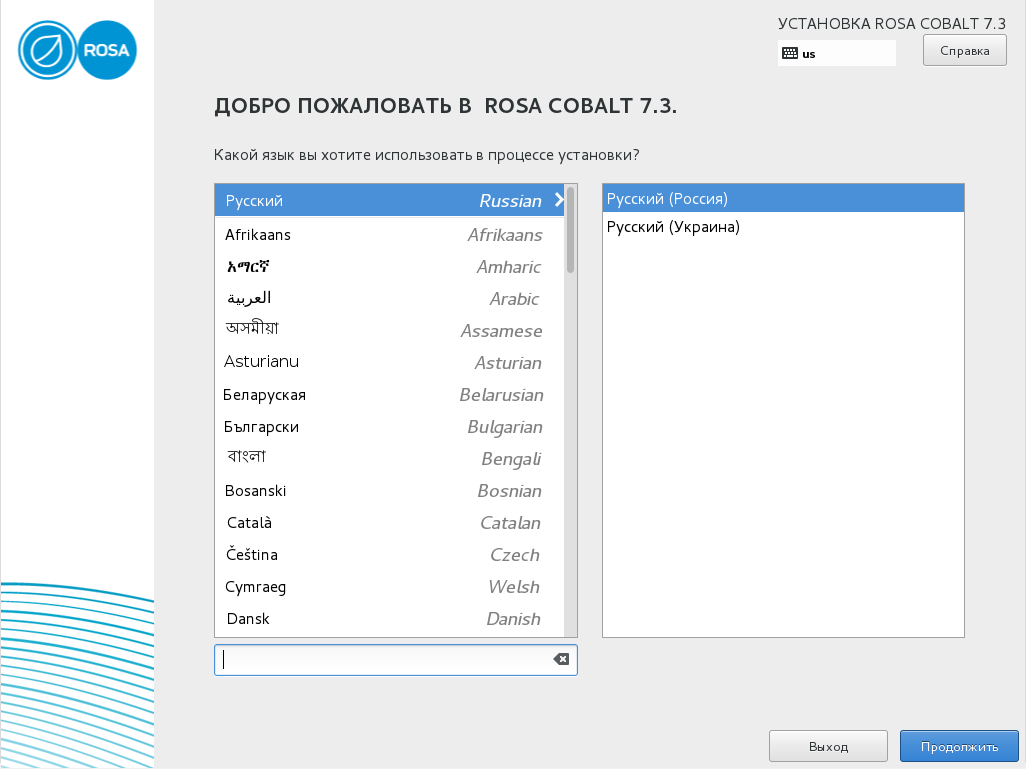
\includegraphics[scale=0.4]{0001.png}
\centering
\caption{Окно приложения TextMaker}
\end{figure}

\subsection{Панель заголовка}
В верхней части окна приложения расположена панель заголовка.

\begin{figure}[ht]

\includegraphics[scale=0.4]{0002.png}
\centering
\end{figure}
Панель заголовка показывает имя приложения и название текущего документа.

Если документ содержит ещё не сохранённые изменения, рядом с названием документа будет показана звёздочка.
\subsection{Панель меню}
Панель меню располагается непосредственно под панелью заголовка.

\begin{figure}[ht]

\includegraphics[scale=0.8]{0003.png}
\centering
\end{figure}
Эта панель содержит все команды TextMaker в виде чётко сгруппированных меню. Нажмите на пункт меню чтобы открыть меню и запустить команду.

\subsubsection{Контекстное меню}
Кроме того, доступно меню, называемое <<контекстным>>.

В этом меню можно найти разные команды, в зависимости от текущего момента. Например, если выделить текст и затем открыть контекстное меню, там будут присутствовать команды для вырезания, копирования или форматирования выделенного текста.

\begin{figure}[ht]
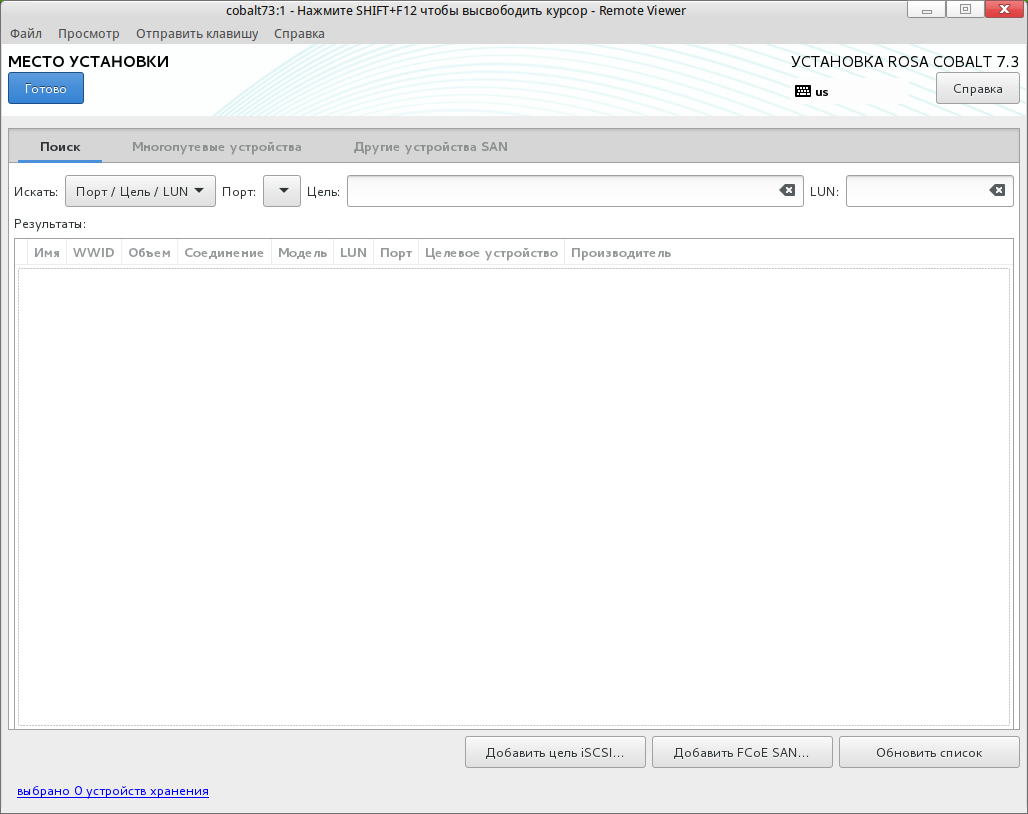
\includegraphics[scale=0.4]{0004.png}
\end{figure}

Чтобы открыть контекстное меню, обычно сначала в документе выделяют како-то элемент/текст, и затем делают щелчок правой клавишей мышки по этому элементу.

Android: в версии для Android также можно открыть контекстное меню пальцем. Коснитесь экрана и затем не отнимайте палец от экрана примерно в течение секунды.

\subsection{Стандартная панель инструментов}

Стандартная панель расположена под панелью меню. На этой панели расположены значки для наиболее часто применяемых действий. При нажатии на значок запускается соответствующая команда.


\includegraphics[scale=0.5]{00012.png}

Панели инструментов, такие, как Стандартная панель, предоставляют быстрый доступ к функциям программы. Каждый значок представляет конкретную команду. При нажатии на значок вызывается соответствующая команда.

\begin{mdframed}[backgroundcolor=blue!10]
\textbf{Совет:} если направить курсор мыши на значок (без нажатия) и удерживать в этом положении,  будет показана так называемая «всплывающая подсказка». Эта подсказка описывает действие, запускаемое при нажатии на значок. 
\end{mdframed}

В TextMaker существуют дополнительные панели инструментов, которые можно включать и отключать по желанию. Для этого либо нажмите на пункт меню \textbf{Вид>Панели инструментов} либо нажмите правой клавишей мышки по одной из видимых панелей. Будет выведено меню, в котором можно выбрать, какие панели должны показываться.

\textbf{Настройка панелей:} набор панелей по умолчанию можно изменять по желанию, а также можно создавать собственные панели. Подробности см. в разделе \nameref{sec:настрпанинстр}.

\subsection{Панель форматирования}
Под Стандартной панелью находится Панель форматирования. С её помощью пользователь может проверить и изменить наиболее часто используемые форматы (шрифт, полужирный шрифт, курсив и т.п.) для текущего текста.


\includegraphics[scale=0.4]{00013.png}

Если фрагмент текста был выделен заранее, изменения в форматировании применяются только к этому выделенному тексту. В противном случае, изменения будут применены к тексту, который будет набираться далее.

Чтобы, например, выбрать другой шрифт, нажмите на маленькую стрелку справа от названия шрифта, чтобы открыть список шрифтов, и выберите нужный шрифт.

Другие значки на панели форматирования — это переключатели, активируемые нажатием мышки, например, \textbf{B} для полужирного шрифта.

\subsection{Окно документа}
Окно документа, используемое для редактирования документа, занимает большую часть экрана.

Каждый документ, который открывает или создаёт пользователь, показывается в своём собственном окне, что предоставляет возможность работы с несколькими документами одновременно, и перемещать данные между этими документами.

Чтобы узнать больше о работе с окнами документов, см. раздел \nameref{sec:окнодокументов}.

Окно документа состоит из следующих элементов:

\subsubsection{Горизонтальная линейка}
Горизонтальная линейка располагается в верхней части окна документов. Здесь показываются поля и шаг табуляции для активного параграфа, или для всех параграфов, которые могут быть выбраны в указанный момент. Единица измерения — дюйм или сантиметр, в зависимости от системных настроек.


\includegraphics[scale=0.5]{0007.png}

Отступы и шаг табуляции не только показываются, их также можно изменять с помощью мыши. Об этом можно узнать в разделе \nameref{sec:отступы} и \nameref{sec:табуляция}.

\subsubsection{Документ}
Документ как таковой занимает большую часть окна документа.

\subsubsection{Боковая панель}
Панель с правой стороны документа, называемая «боковой панелью», — это очень полезный инструмент:

С её помощью, например, можно увидеть список всех заголовков в документе. Если сделать двойной щелчок на одному из элементов документа, TextMaker немедленно перемещается на соответствующий заголовок.

Значки на маленькой панели в верхней части боковой панели дают возможность выбрать, что именно должно показываться в боковой панели (навигатор, стили символов или параграфов).

Боковую панель можно в любое время включить или отключить с помощью пункта меню «Вид>Боковая панель». Там, где можно изменить расположение боковой панели или спрятать её, открывается подменю.

\textit{FreeOffice}: в SoftMaker FreeOffice боковая панель активируется автоматически при запуске программы, на ней показывается познавательная информация про SoftMaker Office.
Чтобы получить больше информации о боковой панели и её отдельных возможностях, см. следующие разделы:
\begin{itemize}
 \item \nameref{sec:навигдокспомбоковпан}
 \item \nameref{sec:стилисимвибокпанель}
 \item \nameref{sec:стилиабзибокпан}
\end{itemize}

\subsubsection{Строка состояния}
Строка состояния располагается в нижней части окна программы.

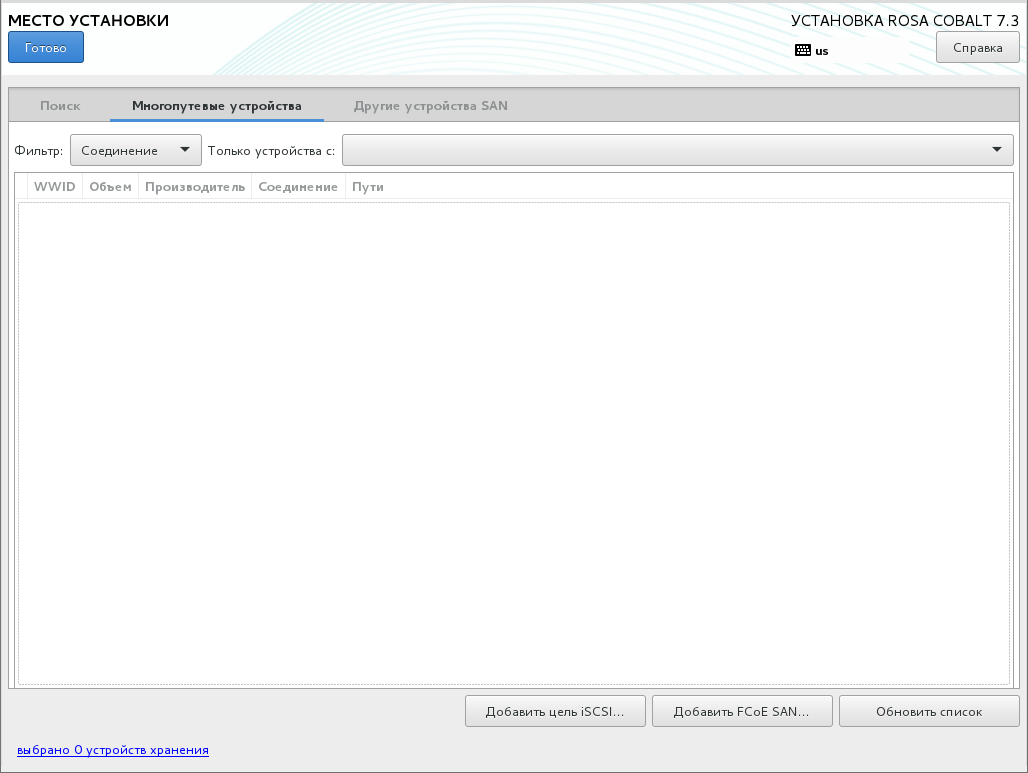
\includegraphics[scale=0.5]{0008.png}

\begin{mdframed}[backgroundcolor=blue!10]
\textbf{Подсказка:} при наведении курсора мыши на значок панели инструментов или команду меню, в строке состояния появляется краткое описания функционала этого значка или команды. 
\end{mdframed}

Кроме того, в строке состояния показывается следующая информация (слева направо):

\begin{center}
\begin{tabular}{ | m{4cm} | m{10cm} | }
\hline
 \textbf{Пример} & \textbf{Объяснение} \\ 
 \hline
 Стр.10 Кол.58 & Текстовый курсор расположен на строке 10 в колонке 58 текущей страницы. \\  
 \hline
 Раздел 1 & Текстовый курсор расположен в разделе 1 документа (см. раздел \nameref{sec:многразмстр}) \\
 \hline
 Глава 1 & Текстовый курсор расположен в главе 1 документа (см. раздел \nameref{sec:разелдокнаглавы}). \\
 \hline
 Страница 1 из 2 & Текстовый курсор расположен на странице 1 документа, состоящего из двух страниц. \\
 \hline
 Русский & Текст в текущей позиции курсора (или текущий выделенный текст) набран на Русском языке (см. также \nameref{sec:установкаязыка}).\\
 \hline
 Вст & Показывает, какой из режимов набора текста активен, вставка (Вст) или замена (Зам):
\textbf{Вст:} активен режим вставки — вводимый текст вставляется в существующий текст.
\textbf{Зам:} активен режим замены — вводимый текст заменяет существующий текст.
По умолчанию установлен режим вставки. Переключение между двумя режимами происходит с помощью клавиши Insert.\\
\hline
\end{tabular}
\end{center}

\section{Базовые операции} \label{sec:бо}
В этой главе пользователь может познакомиться с кратким описанием наиболее важных базовых функций TextMaker. 

После этого рекомендуется обратиться к следующей главе, \nameref{sec:tmвп}, чтобы шаг за шагом применить полученные знания на практических примерах.

\subsection{Ввод текста}
При запуске TextMaker автоматически открывается окно пустого документа, и пользователь может начинать водить текст без промедления. Не беспокойтесь, если вы умеете пользоваться пишущей машинкой, то без проблем освоите TextMaker.

\begin{mdframed}[backgroundcolor=blue!10]
\textbf{Внимание:} при работе на пишущей машинке в конце каждой строки нужно нажимать клавишу \keys{Enter}. В текстовом процессоре этого делать не нужно. Если вводимое слово не помещается в текущей строке, TextMaker автоматически перенесёт его на следующую. Клавишу \keys{Enter} нужно нажимать только в следующих случаях:
\end{mdframed}

\begin{itemize}
 \item чтобы закончить абзац
 \item чтобы ввести пустую строку
\end{itemize}

Поэтому, находясь внутри абзаца, предоставьте TextMaker делать правильные окончания строк.

\subsection{Перемещение текстового курсора}
При наборе и редактировании текста мы всегда видим мигающую чёрточку. Это так называемый текстовый курсор. При наборе текстов, буквы всегда появляются там, где расположен текстовый курсор.

Текстовый курсор можно расположить в любом месте между началом и концом документа. Для этого существуют клавиши со стрелками. Клавиши \keys{\arrowkeyleft} и \keys{\arrowkeyright} , например, передвигают курсор на один символ влево и вправо, соответственно.

Все доступные клавиши, применяемые для перемещения курсора:

\begin{center}
\begin{tabular}{  m{2cm}  m{12cm}  }
\keys{\arrowkeyleft} & На один символ влево \\ 
\keys{\arrowkeyright} & На один символ вправо\\
\keys{\arrowkeyup} & На одну строку вверх \\
\keys{\arrowkeydown} & На одну строку вниз \\
\keys{Home} & В начало строки\\
\keys{End} & В конец строки \\
\keys{Ctrl}+\keys{\arrowkeyup} & В начало текущего абзаца или, при повторном нажатии, предыдущего\\
\keys{Ctrl}+\keys{\arrowkeydown} & В следующий абзац \\
\keys{Ctrl}+\keys{Home} & В начало документа \\
\keys{Ctrl}+\keys{End} & В конец документа \\
\end{tabular}
\end{center}

Кроме того, расположить текстовый курсор в нужном месте можно нажатием мышки.

\textbf{Android}: в версии для Android также можно произвести касание пальцем в нужной позиции.

\subsection{Удаление текста}
Каждый пользователь время от времени делает опечатки, которые нужно удалять. В TextMaker это можно делать несколькими способами. 

\textbf{Удаление символов:} чтобы удалить символ, используйте клавишу \keys{BackSpace}, расположенную над клавишей \keys{Enter}. Эта клавиша удаляет символ слева от текстового курсора. Последующий текст сдвигается назад автоматически.

Также можно удалять символы в противоположном направлении: за это отвечает клавиша \keys{Delete}, которая удаляет символ не слева, а справа от текстового курсора.

\textbf{Удаление слов:} если расположить текстовый курсор перед первой буквой слова, и затем нажать сочетание клавиш \keys{Ctrl}+\keys{Del}, то это слово будет удалено. Если текстовый курсор расположен в середине слова, то это сочетание клавиш удаляет только оставшиеся буквы слова, следующие после курсора.

\textbf{Удаление возврата каретки:} пользователь также может удалить ошибочно введённый возврат каретки. Проверить это можно следующим способом: напечатайте абзац из нескольких строк и затем посредине абзаца введите возврат каретки, нажав клавишу \keys{Enter}. Дальнейший текст перемещается на следующую строчку, и абзац разделяется. В некоторых случаях, когда абзац слишком объёмный, и его нужно  разделить на два, это можно сделать намеренно. Но в данном случае это была «ошибка», поэтому — нажмите клавишу \keys{BackSpace} для удаления возврата каретки.

\textbf{Удаление больших фрагментов текста:} вышеописанные клавиши удаления удобны для удаления небольших фрагментов текста, но удаление таким способом объёмных фрагментов текста занимает слишком много времени. Поэтому существует ещё один способ удаления текста, когда необходимый фрагмент сначала выделяется, а затем, например, нажимается клавиша \keys{Del}, для мгновенного удаления всего выделенного текста. Больше информации об этом можно найти в главе \nameref{sec:рсв}.

\subsection{Отмена изменений} \label{sec:отменаизм}
TextMaker — программа, прощающая ошибки, и позволяющая отменить самые свежие изменения с помощью команды \textbf{Правка>Отменить}. Если пользователь, например, удалил некоторый текст, а затем решил, что этот текст нужно вернуть, всё, что ему нужно сделать, это вызвать пункт меню \textbf{Правка>Отменить}, и удаление будет отменено.

Этот способ применим не только для удалений, но практически для любого типа изменений, внесённых в документ, например, для вставки объекта в тест.

Команду \textbf{Отменить} можно применять несколько раз подряд, например, для отмены пяти последних изменений текста.

Команду \textbf{Отменить} можно также вызывать сочетанием клавишей \keys{Ctrl}+\keys{Z}.

\subsubsection{Повторение отменённых действий}
Также существует команда, действие которой противоположно команде Отмена, это команда \textbf{Правка>Вернуть}. Эта команда восстанавливает результат отменённого действия.

Для этой команды также есть сочетание клавиш: \keys{Ctrl}+\keys{Y}.

\subsection{Ввод или замена?}
Ввод текста осуществляется очень просто. Пользователь помещает текстовый курсор в нужное место и начинает печатать.

По умолчанию, в TextMaker включен режим Ввод. Если в этом режиме напечатать символ, символ вводится в существующий текст и смещает последующий текст вперёд.

Можно также переключиться в режим Замена. В этом режиме вводимый текст заменяет (перезаписывает) последующий текст.

Строка состояния всегда показывает, какой из двух режимов включен в данную минуту: \textbf{Вст} означает режим ввода, \textbf{Зам} — пользователь работает в режиме замены.

Переключение между этими двумя режимами осуществляется с помощью клавиши \textbf{Insert}.

\subsection{Создание нового документа}
Чтобы создать новый документ, вызовите пункт меню \textbf{Файл>Новый}, или нажмите сочетание клавиш \keys{Ctrl}+\keys{N}.

\begin{figure}[ht]
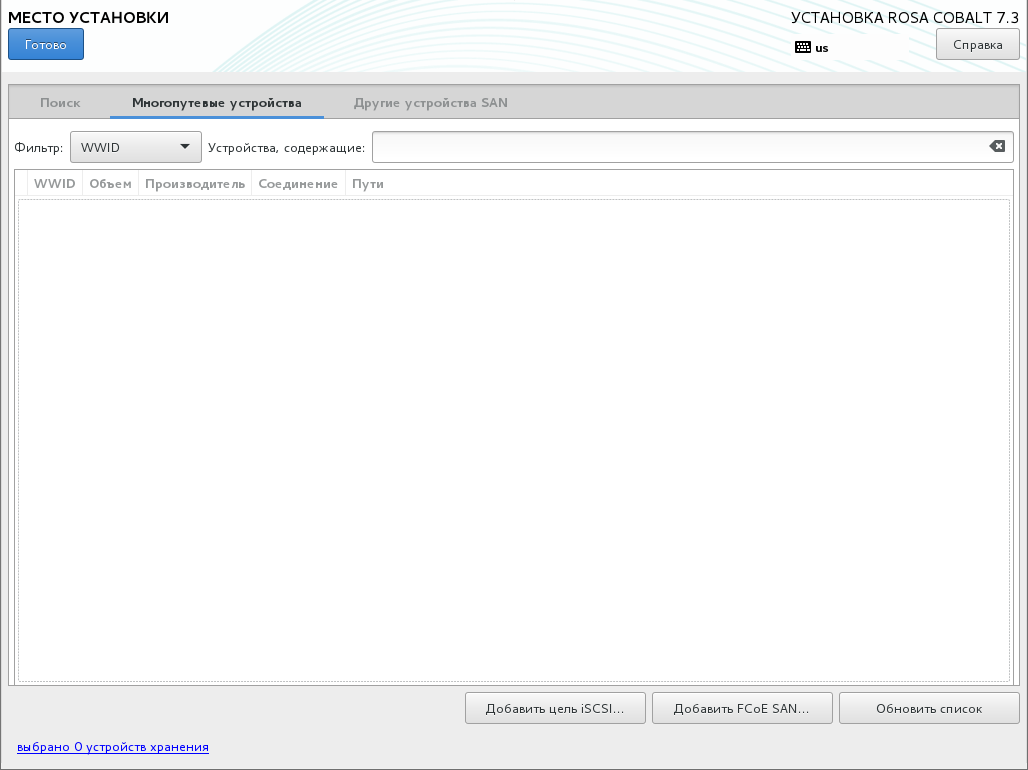
\includegraphics[scale=0.5]{0009.png}
\centering
\caption{Диалоговое окно меню Файл>Новый}
\end{figure}

Появится диалоговое окно, в котором можно выбрать шаблон для нового документа. 

Если пользователю просто нужно создать новый документ, без срочной необходимости выбора шаблона, то мы рекомендуем стандартный шаблон NORMAL.TMV.

После нажатия кнопки OK параметры нового документа будут настроены.

\subsubsection{Использование шаблонов документов}
Кроме стандартного шаблона NORMAL.TMV пользователю также доступны несколько папок, которые можно открыть двойным нажатием мыши. В папках находятся подготовленные шаблоны для писем, факсов и т.п. Далее их просто нужно наполнить содержимым.

\begin{mdframed}[backgroundcolor=blue!10]
\textbf{Совет:} в правой части диалогового окна показывается предварительный просмотр выбранного шаблона. Показ предварительного просмотра можно в любое время включить или выключить с помощью кнопки >> или << . (Эта возможность отсутствует в SoftMaker FreeOffice.) 
\end{mdframed}

Подробную информацию о работе с шаблонами документов см. в разделе \nameref{sec:шаблоныдокументов}.

\subsubsection{Параметр «Новое окно»}
Флажок «Новое окно» в этом диалоге имеет следующее значение: при включенном флажке новый документ будет открыт в новом окне, в противном случае — текущий документ в активном окне будет закрыт, и вместо него будет создан новый документ.

\subsection{Открытие документов} \label{sec:открытиедок}
Чтобы открыть уже существующий документ, вызовите команду из пункта меню \textbf{Файл>Открыть}, или нажмите сочетание клавиш \keys{Ctrl}+\keys{O}.

Появится диалоговое окно, выглядящее примерно так: 

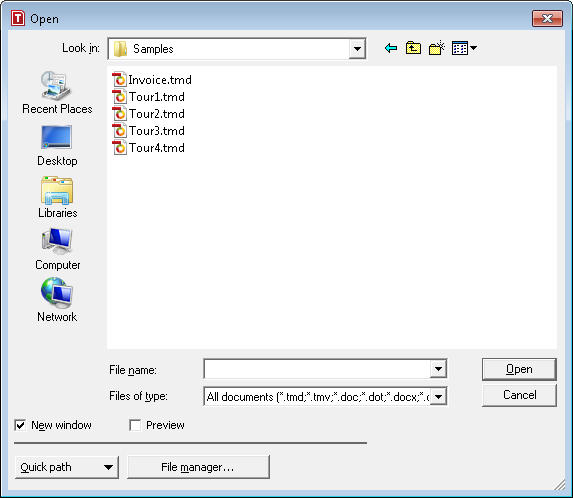
\includegraphics[scale=0.4]{00010.png}

В папке недавно использованных документов будет список всех существующих документов (отсортированных по типу файла). Чтобы выбрать файл для открытия, введите его имя вручную или просто выберите файл из списка. Затем нажмите на кнопку «Открыть».

\textbf{Новое окно}: чтобы открыть документ в новом окне, отметьте флажком параметр «Новое окно». В противном случае, текущий документ будет закрыт, и в этом же окне будет открыт новый.

\subsubsection{Открытие файлов в других форматах}
В дополнение к файлам, созданным в стандартном файловом формате TextMaker, в программе можно открывать файлы, созданные в других программах, например, в Microsoft Word. Чтобы открыть файл, созданный в другом приложении,  выберите необходимый формат файла в списке «Тип файла». 

Больше сведений по этой теме можно найти в главе \nameref{sec:рабсдрформатамифайлов}.

\subsubsection{Предварительный просмотр документа}
При отмеченном параметре <<Предварительный просмотр>>, в небольшом блоке рядом с диалогом выбора файла присутствует предварительный просмотр документа.

\subsubsection{Использование быстрых путей}
С помощью кнопки «Быстрый доступ» можно создать быстрые пути для ускорения перемещения в конкретную папку при открытии или сохранении файлов. Это даёт возможность создать список наиболее часто используемых папок для быстрой навигации.

Подробности см. в разделе \nameref{sec:быстрыйдоступ}.

\subsubsection{Использование менеджера файлов}
\begin{mdframed}[backgroundcolor=pink!50]
\textbf{\textit{FreeOffice}:} этот функционал отсутствует в \textbf{SoftMaker \textit{FreeOffice}}.
\end{mdframed}

Кнопка «Менеджер файлов» открывает встроенный менеджер файлов, который показывает список документов пользователя с возможностью открыть, распечатать, просмотреть или удалить документ. Также есть возможность поиска.

Подробности см. в разделе \nameref{sec:менеджфайлов}.

\subsubsection{Использование списка недавно использовавшихся файлов}
\textit{\textbf{Совет}}: в нижней части меню «Файл» находится список недавно открывавшихся файлов. Чтобы открыть такой файл снова, просто нажмите на него.

\subsection{Печать документов}
Чтобы распечатать активный документ, выберите команду \textbf{Файл>Печать} или используйте сочетание клавиш \keys{Ctrl}+\keys{P}.

Появится диалоговое окно, в котором можно указать страницы и число копий для печати. По умолчанию, печатается одна копия полного документа.

Подробности о выводе документов (печать, отправка по почте и т.д.) см. в главе \nameref{sec:выводдокументов}.

\subsection{Сохранение документов} \label{sec:сохранениедок}
При работе над документом рекомендуется его время от времени сохранять.

Для сохранения файла можно использовать команду \textbf{Сохранить} из меню \textbf{Файл}, или сочетание клавиш \keys{Ctrl}+\keys{S}. При использовании одного из этих двух способов, документ в активном окне сохраняется под  текущем именем.

Если у документа ещё нет имени, TextMaker автоматически предложит указать имя документа при открытии диалогового окна \textbf{Сохранить как}.

\subsubsection{Сохранение под другим именем или по другому пути}
Чтобы сохранить документ под другим названием или в другом местоположении, используйте команду \textbf{Файл>Сохранить как}. Это действие также сохраняет все внесённые в файл изменения, но пользователь должен сначала указать другое имя файла или другую папку для сохранения.

\subsubsection{Сохранение в другом формате файла}
С помощью меню \textbf{Файл>Сохранить как}, документ можно также сохранить в другом формате. Для этого, перед тем, как нажать на кнопку «Сохранить», просто выберите нужный формат файла из списка «Тип файла». Также см. главу \nameref{sec:рабсдрформатамифайлов}.

\subsubsection{Сохранение всех открытых документов}
Если у пользователя открыто несколько окон документов одновременно, для сохранения всех документов, открытых во всех окнах, можно использовать команду \textbf{Файл>Сохранить все}. TextMaker проверяет, какие из документов были изменены с момента последнего сохранения, и сохраняет только те, которые были изменены.

\subsubsection{Выход из приложения}
Чтобы выйти из программы TextMaker, используйте команду \textbf{Файл>Выход}.

Если какие-либо из открытых документов были изменены со времени их последнего сохранения, TextMaker автоматически спросит, нужно ли их сохранить.

\section{TextMaker в примерах} \label{sec:tmвп}
Добро пожаловать в раздел «TextMaker в примерах»!

На следующих страницах, с помощью практических примеров мы представим наиболее важные возможности TextMaker.

\textbf{Внимание}: выполняя задания из примеров, по мере улучшения навыков работы, не бойтесь экспериментировать с новыми командами. Не страшно, если что-то пойдёт не так. Для каждого из заданий мы предоставляем примеры документов, чтобы в начале каждого из уроков пользователь мог открыть соответствующий документ и начал с ним работу.

\begin{mdframed}[backgroundcolor=blue!10]
\textbf{Внимание:} большинство документов для работы с заданиями были подготовлены в версии TextMaker для Windows. В других ОС некоторые элементы управления выглядят несколько иначе, но их функционал полностью идентичен. 
\end{mdframed}

\subsection{Упражнение: деловое письмо}
Готовы для первого задания? Тогда запускайте TextMaker.

\begin{mdframed}[backgroundcolor=blue!10]
\textbf{Внимание:} при первом запуске TextMaker вам будет предложено ввести имя и адрес. Эта информация требуется не для регистрации программы. TextMaker будет использовать эту информацию для автоматической персонализации шаблонов писем, факсов и т.д., входящих в состав программы. Эту информацию всегда можно изменить позже с помощью команды \textbf{Сервис>Параметры} (см. раздел \nameref{sec:парамвклдкаобщие}).
\end{mdframed}

После запуска программы всегда появляется окно пустого документа, в котором можно сразу  начинать печатать. Тестовый курсор мигает в начале документа. Вводимый текст появляется сразу после текстового курсора, который передвигается далее вперёд. 

Для начала, давайте начнём составлять простое письмо от имени ЗАО «Рога и копыта». Просто, но профессионально. В конце данного занятия у нас будет готово полноценное деловое письмо, со всеми полагающимися атрибутами.

На этом этапе пользователь может сказать: «Не проще ли будет применить команду \textbf{Файл>Новый} и выбрать один из готовых шаблонов?» Конечно — но таким образом пользователь ничему не научится. Если вы хотите выполнять задания, им будет необходимо уделить некоторое время, но зато впоследствии вы овладеете самыми главными функциями программы и сможете немедленно изменять шаблоны для ваших нужд.

Итак, давайте начнём. Сначала напечатайте какой-нибудь текст, похожий на указанный ниже. (Копировать его буквально не обязательно, подойдёт любой текст с произвольным содержимым.)

\begin{mdframed}[backgroundcolor=blue!10]
\textbf{Важно:} нажимайте на клавишу \keys{Enter} только в указанных местах. При использовании текстового процессора не нужно нажимать эту клавишу в конце каждой строки, как это делается при работе с пишущей машинкой. \keys{Enter} необходимо нажимать только для указания конца абзаца или для вставки пустых строк.
\end{mdframed}

\begin{center}
\begin{tabular}{ | m{15cm} | }
\hline
 Дорогие клиенты! \keys{Enter} \\ 
 \keys{Enter} \\
 За прошедшие годы произошло много изменений. Мы наблюдали, как компании приходят и уходят, люди приезжают и уезжают, технический прогресс меняет планету. Чтобы идти в ногу со временем, ЗАО «Рога и Копыта» решило изменить свое имя на ООО «Любовь и голуби».\keys{Enter} \\
 Это изменение в названии более точно отражает нашу компанию и продукты, которые мы предлагаем. Единственное отличие для вас — это смена названия.\keys{Enter} \\
 \keys{Enter} \\
 Мы так же, как и прежде, рады предложить вам ту же самую высококачественную продукцию по прежним и приемлемым ценам.\keys{Enter} \\
 \keys{Enter} \\
\hline
\end{tabular}
\end{center}

\textbf{Ошибки при вводе текста:} допущенные опечатки можно сразу же удалять, нажимая клавишу \keys{BackSpace}. Эта клавиша расположена над клавишей \keys{Enter}.

Если вы придерживались примера, то готовый текст должен выглядеть примерно так:

\pagebreak

\begin{figure}[ht]
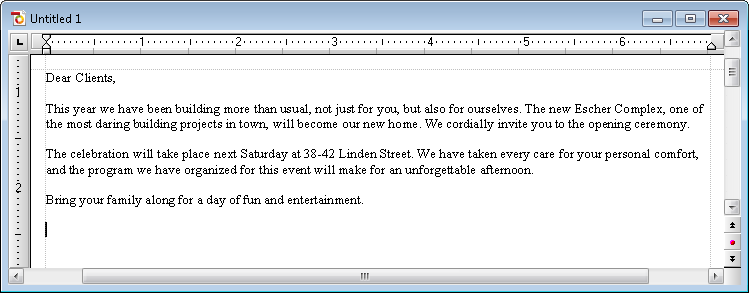
\includegraphics[scale=0.4]{00011.png}
\centering
\caption{Готовый текст}
\end{figure}

Далее, нам нужно ввести \index{адрес} над текстом нашего письма. Чтобы переместиться в начало документа, нажмите \keys{Ctrl}+\keys{Home}.

Нажмите клавишу \keys{Enter} семь раз, чтобы ввести несколько пустых строк. Мы создали место для адреса нашей компании, который будет введён позже. Кстати, лишние пустые строки можно удалить с помощью клавиши \keys{BackSpace}.

Далее, нажмите один раз клавишу \keys{\arrowkeyup} чтобы расположить текстовый курсор в пустой строке над текстом письма.

Теперь введите адрес и имя человека, которому адресовано письмо:

\begin{center}
\begin{tabular}{ | m{15cm} | }
\hline
1223456, Санкт-Петербург, \keys{Enter} \\
Гражданская ул., дом 19\keys{Enter} \\
Раскольникову Р.Р.\keys{Enter} \\
\hline
\end{tabular}
\end{center}

Далее, введите дополнительные пустые строки, нажав клавишу \keys{Enter} одиннадцать раз, чтобы создать пустое пространство между адресом и текстом письма.

Мы создали наиболее важные элементы простого письма и на этом этапе хотим сохранить его.

\subsection{Сохранение письма-задания}
\textbf{Внимание:} подробную информацию по этой теме можно найти в разделе \nameref{sec:сохранениедок}.

Чтобы сохранить текущий документ, используйте команду \textbf{Сохранить} из меню \textbf{Файл}. (Далее мы будем использовать обозначение \textbf{Файл>Сохранить}.) Вызовите эту команду следующим образом:

\textbf{\textit{Мышь}}: нажмите на кнопку \textbf{Файл} на панели меню. Откроется меню \textbf{Файл}, в котором вызвать команду \textbf{Сохранить} можно нажатием мыши.

\textbf{\textit{Клавиатура}}: для вызова команд пользователи ПК могут также использовать подчёркнутые буквы в меню. Введите подчёркнутую букву, одновременно удерживая клавишу \keys{Alt}. Например, чтобы сохранить файл, нажмите \keys{Alt}+\keys{Ф} для \textbf{\underline{Ф}айл}, а затем \keys{С} для \textbf{\underline{С}охранения}. 

Во время работы вы, возможно, заметили, что \keys{Ctrl}+\keys{S} показывается справа от команды \textbf{Сохранить}. Это является горячим сочетанием клавиш для этой команды, т.е., для вызова этой команды и сохранения документа можно также использовать данное сочетание клавиш.

Для работы с мышью также существует быстрый вызов команд — на стандартной панели расположены значки для наиболее часто используемых команд. 


\includegraphics[scale=0.6]{00012.png}

Для сохранения документа нажмите на значок дискеты на стандартной панели инструментов (третий значок слева).

\begin{mdframed}[backgroundcolor=blue!10]
\textbf{Совет:} если направить курсор мыши на значок (без нажатия) появится текстовый блок, описывающий действие, запускаемое при нажатии на значок.
\end{mdframed}

Если стандартная панель не показывается, она, возможно, отключена. Чтобы включить её снова, вызовите команду \textbf{Вид>Панели инструментов} и отметьте галочкой \textbf{Стандартную} панель. 

\subsubsection{Диалоговое окно «Сохранить»}
Если письмо не имеет названия, при вызове пункта меню \textbf{Файл>Сохранить}, программа автоматически показывает диалоговое окно с просьбой указать имя файла. Введите имя файла в поле \textbf{Имя файла}, или, если необходимо перезаписать уже существующий файл, выберите имя из списка файлов.

Мы назовём наш документ ПИСЬМО. Поэтому, введите название «ПИСЬМО» в поле \textbf{Имя файла} и нажмите кнопку \textbf{OK} или клавишу \textbf{Enter} для подтверждения. TextMaker сохранит файл под указанным именем и автоматически присвоит ему расширение .TMD (“TextMaker document”). Таким образом мы получим полное имя файла ПИСЬМО.TMD.

В следующий раз, когда мы вызовем меню \textbf{Файл>Сохранить}, диалоговое окно уже не появится, поскольку у документа уже есть имя, и он будет немедленно сохранён под этим именем.

Кстати, выйти из диалога сохранения файла можно без выполнения команды \textbf{Сохранить}. Это можно сделать, нажав на кнопку \textbf{Отменить} вместо кнопки \textbf{OK} на контрольной панели или нажав клавишу \keys{Esc}. Этот способ доступен пользователю во всех диалоговых окнах.

\subsection{Простое форматирование}
Далее, мы приближаемся к более интересным функциям, например, к форматированию текста, а, соответственно, к применению шрифтов, визуального выделения (полужирный шрифт, курсив и т.д.), расстановке абзацев и так далее.

Сначала мы вставим строку для обратного адреса над адресом получателя, как это обычно делается для писем, отсылаемых в специальных конвертах с «окошками».

Поэтому давайте расположим курсор двумя строками выше адреса (строка 5) и введём адрес фирмы:

\begin{center}
\begin{tabular}{ | m{15cm} | }
\hline
ООО «Любовь и голуби»,  оборудование для аквариумов. г.Рыбокочинск, ул.Капитана Врунгеля, дом 2\\
\hline
\end{tabular}
\end{center}

\subsubsection{Сначала выделяем, потом форматируем}
\textbf{Внимание:} подробности выделениях можно найти в главе \nameref{sec:рсв}.

Чтобы форматировать фрагмент текста после того, как текст был введён, сначала его нужно выделить, чтобы TextMaker узнал, какую область необходимо форматировать.

Чтобы выделить строки, в которых содержится адрес, сделайте следующее:

\textbf{\textit{Мышь}}: нажимая и не отпуская кнопку мыши, перетащите курсор мыши от начала до конца текста, который нужно выделить. Кстати, существует простой способ выделить строку — нажмите мышкой на поле слева от  строки, и вся строка целиком будет выделена.

\textbf{\textit{Клавиатура}}: пользователи, предпочитающие работу с клавиатурой, могут выделять текст, передвигая текстовый курсор, удерживая клавишу \keys{Shift}. В этом случае выделите строку адреса, с помощью клавиши \keys{Home} поместив курсор перед первым символом и затем нажав сочетание клавиш \keys{Shift}+\keys{\arrowkeydown}.

\begin{mdframed}[backgroundcolor=blue!10]
\textbf{Android:} обратите внимание, что в версии для Android выделение текста производится другим способом. Подробности см. в разделе \nameref{sec:выделтекстаиобъект}.
\end{mdframed}

После того, как мы выделили строку адреса, можно изменять размер шрифта. Для этого используйте панель форматирования, где находятся все наиболее часто используемые команды форматирования. Если эта панель не показывается, вызовите команду \textbf{Вид>Панели инструментов} и отметьте параметр \textbf{Форматирование}.

\subsubsection{Панель форматирования}
\textbf{\textit{Внимание}}: подробную информацию о панели форматирования можно найти в главе \nameref{sec:фс} и \nameref{sec:фа}.


\includegraphics[scale=0.5]{00013.png}

Размер шрифта выделенного текста показывается справа от названия шрифта — на иллюстрации выставлен размер в 10 пт. Нажмите мышью на маленькую стрелку справа от цифры 10 чтобы открыть список наиболее часто используемых  размеров шрифтов. Выберите из списка «8».

Теперь выберем другой тип шрифта. Для этого нажмите на стрелку справа от шрифта и выберите в списке Times New Roman. Если этот шрифт не был установлен, выбирайте любой понравившийся шрифт.

После внесения этих изменений панель форматирования будет выглядеть таким образом:


\includegraphics[scale=0.6]{00014.png}

Был установлен шрифт Times New Roman размером 8 пт.

Далее нам нужно выделить город и почтовый индекс адресата полужирным шрифтом. Выберите строку с городом и индексом в адресе получателя и затем нажмите на букву \textbf{B} на панели Форматирования — или нажмите сочетание клавиш \keys{Ctrl}+\keys{B}. Шрифт строки станет полужирным.

Кстати, выделение текста курсивом делается так же просто, с помощью значка \textit{I} или сочетания клавиш \keys{Ctrl}+\keys{I}; подчёркнутый шрифт форматируется с помощью значка \underline{U} или сочетания клавиш \keys{Ctrl}+\keys{U}. Чтобы сделать обратные  изменения, применяются те же самые средства.

В итоге, адреса получателя и отправителя должны выглядеть примерно таким образом:

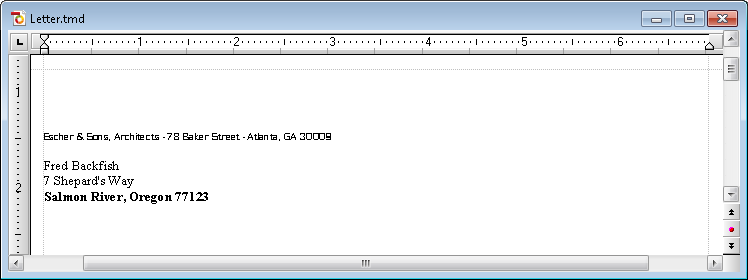
\includegraphics[scale=0.4]{00015.png}

Теперь снова необходимо сохранить наш документ с помощью \textbf{Файл>Сохранить}.

\subsection{Если что-то пошло не так…}
\textbf{Внимание:} подробную информацию по этой теме можно найти в разделе \nameref{sec:отменаизм}.

Как мы видели в предыдущем задании, снять полужирное форматирование можно, снова применив этот атрибут шрифта к тексту, уже выделенному полужирным.

В TextMaker есть дополнительная, очень удобная возможность отмены самых свежих изменений с помощью команды \textbf{Правка>Отменить}. Например, если текст был форматирован с помощью другого шрифта, всё, что нужно сделать — это вызвать меню \textbf{Правка>Отменить}, и изменения будут отменены.

Этот способ применяется не только для форматирования, но также практически для вех типов изменения — например, можно отменить ввод абзаца или удаление текста.

Команду \textbf{Отменить} можно последовательно применять столько раз, сколько необходимо. Например, вызовите её пять раз, чтобы отменить пять последних внесённых изменений.

Кстати, эту крайне необходимую команду можно вызвать с помощью сочетания клавиш \keys{Ctrl}+\keys{Z}.
Также существует команда, противоположная по действию — это команда \textbf{Правка>Вернуть} (сочетание клавиш \keys{Ctrl}+\keys{Y}). Эта команда восстанавливает последнее отменённое действие. Таким образом, можно отменить отмену действия.

\subsection{Открытие файлов}
\textbf{Внимание}: подробности по этой теме см. в разделе \nameref{sec:открытиедок}.

Теперь мы откроем файл с примером TOUR 1.TMD, прилагающийся к программе. В нём содержится наш документ-задание в таком виде, в каком он должен выглядеть на этом этапе нашей работы.

Чтобы открыть документ, вызовите команду \textbf{Файл>Открыть} из меню или с помощью сочетания клавиш \keys{Ctrl}+\keys{O}. 

Сначала перейдем в папку, где лежат документы-примеры. Чтобы её найти, выполните следующие действия:
\begin{itemize}
 \item В ОС Windows 7 или более поздних, перейдите в папку пользователя. Дальше, перейдите в папку MY DOCUMENTS \textbackslash SOFT MAKER \textbackslash SAMPLES.
 \item В Windows XP перейдите в папку MY DOCUMENTS \textbackslash SOFT MAKER \textbackslash SAMPLES.
 \item В Linux перейдите в домашний каталог пользователя и оттуда — в каталог SOFT MAKER/SAMPLES.
 \item На устройстве Android прейдите в папку SOFT MAKER/SAMPLES на карте SD. В этой папке найдите TOUR 1.TMD и сделайте двойное касание по файлу для его открытия.
\end{itemize}

\subsection{Настройка верхнего колонтитула письма}
Конечно, нашему письму необходима достойно выглядящая «шапка», с названием компании большим шрифтом и, возможно, с описанием, какие продукты или услуги предлагает наша компания.

За работу! С помощью сочетания клавиш \keys{Ctrl}+\keys{Home} переместите текстовый курсор в начало документа TOUR 1.TMD, который мы только что открыли. Теперь введите:

\begin{center}
\begin{tabular}{ | m{15cm} | }
\hline
ООО «Любовь и голуби»\keys{Enter} \\
Оборудование для аквариумов. \\
\hline
\end{tabular}
\end{center}

Название компании вполне можно сделать чуть-чуть побольше размером: выберите первую строку и с помощью панели \textbf{Форматирования} выберите шрифт \textbf{Times New Roman}, размер 32 и сделайте его полужирным.

Размер 32 отсутствует в списке? Не важно, т.к. в списке присутствуют только наиболее часто используемые размеры, но нужный именно вам размер можно ввести вручную. Просто нажмите на размер, показанный в окошке на панели форматирования, введите 32 и подтвердите нажатием клавиши Enter \keys{Enter}.

Кстати, для размера шрифта можно даже указать не целое значение (например, 12.6 пт), в том случае, если текст нужно уместить в ограниченное пространство.
В итоге, панель форматирования должна выглядеть таким образом:

\begin{figure}[ht]

\includegraphics[scale=0.6]{00016.png}
\centering
\caption{Установлен шрифт Times New Roman 32 пт полужирный.}
\end{figure}

Далее нам нужно форматировать шрифт во второй строке шрифтом Times New Roman 12 пт курсив. Для этого нам сначала нужно выделить текст. На этот раз мы не будем использовать панель форматирования, а вызовем \textbf{Формат>Шрифт}, чтобы познакомиться также и с этой часто применяемой командой.

Отроется диалоговое окно, в котором находятся сразу все возможности для форматирования символов.

\begin{figure}[ht]
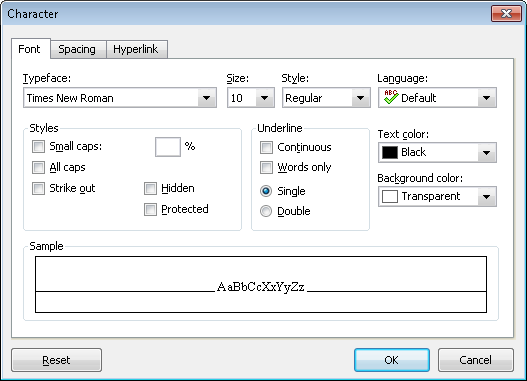
\includegraphics[scale=0.6]{00017.png}
\centering
\caption{Диалоговое окно Формат>Шрифт.}
\end{figure}

\textbf{Внимание}: подробную информацию об этом диалоговом окне можно найти в главе \nameref{sec:фс}.

Параметры диалогового окна распределены по нескольким «индексным карточкам», перейти на которые можно, нажав на вкладки в верхней части окна. Как можно видеть, в этом диалоговом окне есть вкладки \textbf{Шрифт}, \textbf{Интервал} и \textbf{Гиперссылка}. Поскольку нам нужно изменить только шрифт, мы остаёмся только на вкладке \textbf{Шрифт}.

Откройте выпадающий список «Гарнитура шрифта» нажатием на маленькую стрелку справа от названия шрифтов, и выберите шрифт Times New Roman. Затем выберите размер 12 пт в окошке справа от окошка с названиями шрифтов. Включите курсив, открыв выпадающий список \textbf{Стиль} и выбрав пункт \textbf{Курсив}.

Подтвердите выбранные параметры, нажав на клавишу \textbf{Enter}, затем сохраните документ.

\subsection{Выравнивание абзацев}
То, как TextMaker располагает текст между полями документа, называется «выравниванием абзацев».

Режим выравнивания абзацев изменяется с помощью команды \textbf{Формат>Абзац}. При вызове этой команды появляется диалоговое окно. Откройте список \textit{Выравнивание} во вкладке \textbf{Абзац}. Далее, выберите нужный способ выравнивания из списка.

Эту операцию можно выполнить быстрее с помощью панели \textbf{Форматирования}, на которой находятся четыре значка, на которые можно нажать мышью для смены способа выравнивания:


\includegraphics[scale=1]{00018.png} выравнивание слева


\includegraphics{00019.png} выравнивание справа


\includegraphics{00020.png} выравнивание по центру


\includegraphics{00021.png} выравнивание по ширине страницы

Теперь мы разместим название компании по центру страницы. Для этого, переместите текстовый курсор перед любым символом названия компании ООО «Любовь и голуби» и затем нажмите на значок «Выравнивать абзац по центру», на панели форматирования.

\begin{mdframed}[backgroundcolor=blue!10]
\textbf{Внимание:} действия по форматированию абзаца, т.е. все действия форматирования, которые выполняются через меню \textbf{Формат>Абзац}, всегда применяются ко всему абзацу. Так, если необходимо изменить формат отдельного абзаца, его не нужно сначала выделять. Просто разместите текстовый курсор на любую позицию внутри абзаца.
\end{mdframed}

С другой стороны, если необходимо изменить форматирование нескольких последовательно идущих абзацев, их необходимо сначала выделить. Выделение можно начинать с любого места внутри первого абзаца и закончить в любом месте последнего.

Давайте попробуем. Вызовите команду \textbf{Правка>Вернуть}, и название компании снова сдвинется к левому полю документа. Начиная с любой буквы в имени компании, удерживая мышь, перетащите выделение на следующую строку. Затем нажмите на значок выравнивания по центру на панели форматирования. Оба абзаца будут выравнены по центру.

После выполнения этих действий наше окно приложения будет выглядеть примерно таким образом:

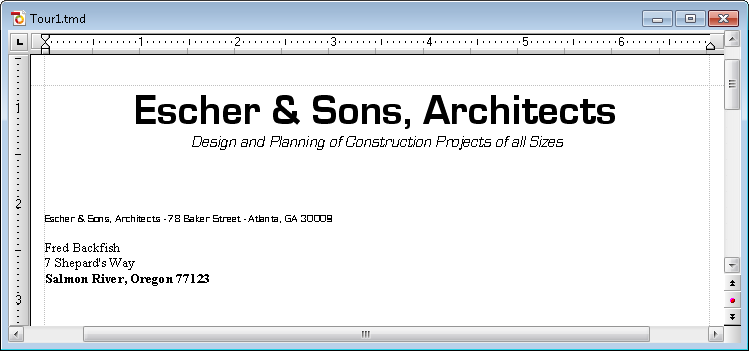
\includegraphics[scale=0.4]{00022.png}

Теперь мы можем напечатать «С наилучшими пожеланиями» внизу письма, и отправить его без лишних колебаний. Но, без сомнения, в письме есть пара элементов, которые можно сделать более привлекательными.

Поэтому давайте приступим к более тонкой отделке.

\subsection{Отступы и табуляция}
Перед тем, как продвигаться дальше, мы откроем документ TOUR 2.TMD и сравним его с нашими достижениями. В этом файле находится наш документ-пример в том виде, как он должен выглядеть на текущем этапе.

Во многие деловые письма включается строка с информацией типа: «Ваш  исходящий номер» или «Ваше письмо от» и так далее. Теперь мы вставим такую строку в наше письмо и в процессе этого познакомимся с применением отступов и табуляции.

\begin{mdframed}[backgroundcolor=blue!10]
\textbf{Внимание:} отступы вставляются с помощью клавиши \keys{Tab}. Хотя на большинстве клавиатур эта клавиша промаркирована значком \Tab, в нашем руководстве мы применяем обозначение \keys{Tab}, чтобы его было проще отличить от обозначений клавиш со стрелками.
\end{mdframed}

Теперь поместите текстовый курсор в начало строки 17 и введите следующее:

\begin{center}
\begin{tabular}{ | m{15cm} | }
\hline
Ваш исходящий номер: \keys{Tab} Ваше  письмо от: \keys{Tab} Наш исх. номер: \keys{Tab}  Наше письмо от: \keys{Tab}  Дата:\\
\hline
\end{tabular}
\end{center}

Потом отформатируйте эту строку шрифтом \textbf{Times New Roman} с размером в 8 пт.

Мы вставили отступы в текст, но ещё не определили их точного размера. Для этого нам нужно указать \textit{шаг табуляции}. По умолчанию, в TextMaker шаг табуляции равен 0,5 дюйма (1,27 см), но обычно это значение, перешедшее от пишущих машинок, не применяется.

Шаг табуляции можно настроить с помощью команды \textbf{Формат>Табуляции} или с помощью панели форматирования и \textit{горизонтальной линейки}.
\begin{figure}[ht]

\includegraphics[scale=0.6]{0007.png}
\centering
\caption{Горизонтальная линейка}
\end{figure}

Если горизонтальная линейка в верхней части окна документа отсутствует, её нужно сначала включить с помощью команды \textbf{Вид>Горизонтальная линейка}.

Шаг табуляции настраивается следующим образом:

\begin{enumerate}
 \item \textbf{Выберите абзац, для которого нужно настроить шаг табуляции:}\\
 Если необходимо настроить шаги табуляции для нескольких абзацев, их необходимо сначала выделить, как было описано выше.\\
Выберите только что введенную строку и строку под ней, поскольку шаг табуляции для следующей строки, которую мы заполним позже, должен иметь такое же значение.
\item \textbf{Выберите нужный тип табуляции на панели Форматирования:}\\
С правой стороны панели форматирования находятся четыре различных значка выравнивания табуляции:\\

\includegraphics[scale=1]{00023.png} \textit{слева}\\

\includegraphics[scale=1]{00024.png} \textit{справа (текст заканчивается в месте табуляции)}\\

\includegraphics[scale=1]{00025.png} \textit{по центру (текст располагается по центру позиции табуляции)}\\

\includegraphics[scale=1]{00026.png} \textit{десятичное (цифры выравниваются по десятичному разделителю)}\\
Нажмите на значок левого выравнивания.
\item \textbf{Нажмите на необходимую позицию табуляции на линейке:}\\
Нажмите мышкой на (примерные) позиции в 2,54 см, 7,62 см, 10,16 см и 13,97 см чтобы установить шаги табуляции. Заметьте, как текст корректируется согласно этим параметрам.
\end{enumerate}

Заметьте, что эту же операцию можно выполнить противоположным способом, т.е. определить шаги табуляции до того, как начинать вводить текст, а затем просто ввести текст.

Линейка и текст теперь должны выглядеть примерно следующим образом:

\begin{figure}[ht]
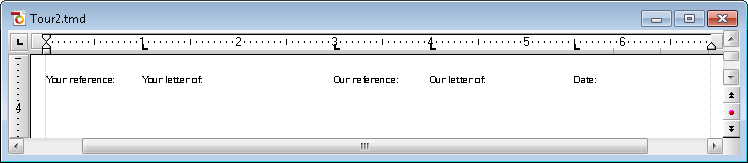
\includegraphics[scale=0.6]{00027.png}
\centering
\caption{Шаги табуляции настроены и показываются на линейке.}
\end{figure}

Если шаг табуляции не устраивает пользователя, его можно изменять прямо на линейке: сначала выделите абзац, в котором нужно изменить табуляцию, затем наведите курсор мышки на указатель шага табуляции и перетащите его на новую позицию на линейке. Не забывайте также, что при перетаскивании указателя табуляции вниз, этот шаг табуляции удаляется.

Существует ещё один способ для установки шагов табуляции. Выделив оба абзаца, вызовите \textbf{Формат>Табуляции}. Будет открыто диалоговое окно, показывающее точные текущие значения шагов табуляции. Настройки в этом диалоге выглядят следующим образом:

\begin{center}
\begin{tabular}{ | m{6cm} | m{6cm} | }
\hline
 \textbf{Цель} & \textbf{Действие} \\ 
 \hline
 Настроить шаги табуляции & Ввести необходимое значение позиции в поле \textbf{Табуляции} и нажать на кнопку \textbf{Установить}.\\
\hline
Удалить шаги табуляции & Выбрать один из существующих шагов табуляции в списке и нажать на кнопку \textbf{Очистить}. Чтобы удалить сразу все позиции, нажать на кнопку \textbf{Очистить все}. \\
\hline
Переместить шаг табуляции & Удалить шаг табуляции и установить новый. \\
\hline
Изменить выравнивание. & Нажать на один из шагов табуляции в списке, выбрать новое выравнивание в списке \textbf{Выравнивание} и нажать на \textbf{Установить}.\\
\hline
\end{tabular}
\end{center}

Для подтверждения изменений нажмите \textbf{OK}.

\textbf{Единицы измерения:} значения в диалоговых окнах TextMaker можно вводить не только в сантиметрах*, но также и в других единицах измерения. Чтобы ввести значение в конкретных единицах, просто добавьте одно из следующих сокращений после числа:

\begin{center}
\begin{tabular}{ | m{4cm} | m{4cm} | }
\hline
 \textbf{Единица измерения} & \textbf{Объяснение} \\ 
 \hline
 см & Сантиметры\\
\hline
дюйм & Дюймы\\
\hline
пт & Пункты \\
\hline
пи & Пики\\
\hline
\end{tabular}
\end{center}

* Единицы измерения по умолчанию зависят от региональных настроек системы.

Вернёмся к нашему письму-уроку.

Теперь, когда были настроены шаги табуляции для строки «ваш исходящий номер» и строки под ней, нам нужно заполнить вторую строку.
Переместите текстовый курсор в начало строки 18 и введите:

\begin{center}
\begin{tabular}{ | m{15cm} | }
\hline
MB\keys{Tab}12.07.16\keys{Tab}HG\keys{Tab}25.09.16\\
\hline
\end{tabular}
\end{center}

Можно убедиться, что поскольку ранее шаги табуляции были настроены для обеих строк, то аналогичные шаги применяются и в этой строке.

В нашем письме отсутствует значение для «сегодняшнего числа». В следующем разделе урока мы настроим TextMaker на автоматическое введение даты и таким образом познакомимся с \textit{полями}.

\subsection{Ввод дат и других полей}
Сегодняшняя дата должна быть указана в области ниже «Даты», значение которой остаётся пока что незаполненным. Естественно, мы не хотим заполнять его вручную, а оставим эту задачу для TextMaker.

После введения текста, указанного выше, введите отступ с помощью клавиши \keys{Tab} и вызовите команду \textbf{Вставить>Поле}.

\pagebreak

\begin{figure}[ht]
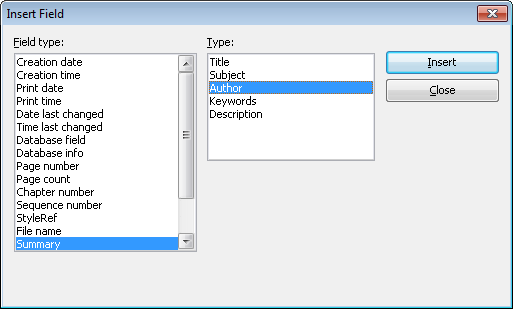
\includegraphics[scale=0.6]{00028.png}
\centering
\caption{Диалоговое окно  Вставить>Поле}
\end{figure}

Из списка Тип поля выберите поле «Дата печати». Справа, в списке Формат даты, можно выбрать формат, в котором будет вставляться дата. Выберите нужный формат и нажмите на кнопку Вставить.

TextMaker вставит текущую дату в текст, и после этого наше письмо будет выглядеть примерно таким образом:

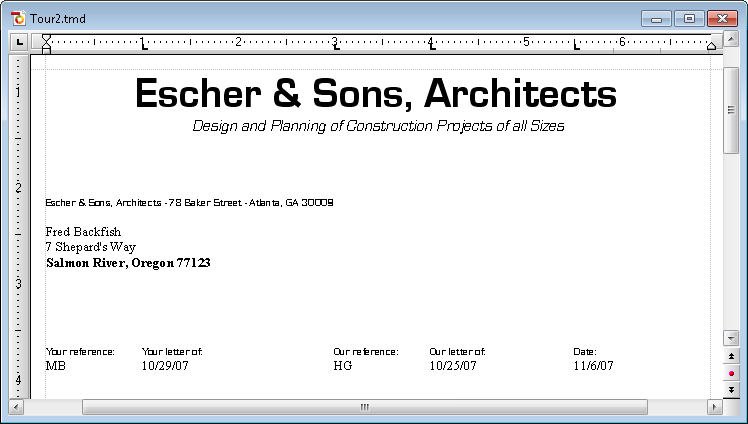
\includegraphics[scale=0.4]{00029.png}

Поля — очень удобный и практичный функционал. Во-первых, мы уже избавились от необходимости вводить текущую дату вручную, во-вторых — поле «дата печати» имеет не фиксированное, а символьное значение, автоматически обновляемое при печати документа. Поэтому, если письмо-урок будет напечатано завтра, то на этом месте будет стоять завтрашнее число.

С помощью полей можно не только вставлять дату, но также выводить текущую станицу документа, имя файла и много другой полезной информации.

Более того, с помощью полей можно вставлять поля баз данных из базы данных, как это требуется для типовых писем.

\subsection{Нижние колонтитулы}
Перед тем, как продолжать,  нам нужно открыть файл TOUR 3.TMD. В нём содержится пример документа в том виде, в каком он должен быть на этой стадии задания.

Настроить верхний и нижний колонтитулы можно для каждого документа: шапка будет печататься наверху страницы, а нижний колонтитул — внизу, на каждой странице. 

За нижние колонтитулы отвечает команда \textbf{Вставить>Нижний колонтитул}. При её вызове текстовый курсор располагается в нижней границе страницы. Это область, куда можно вводить нижний колонтитул.

Сейчас мы выберем шрифт Times New Roman 8пт перед тем, как начать вводить текст. Выберите этот шрифт с помощью панели форматирования. Теперь вводимый текст уже появится отформатированный в этом шрифте.

Давайте введём в нижнем колонтитуле адрес нашей компании и некоторую дополнительную информацию, например, сведения о банке, обслуживающем компанию. Конечно, необязательно следовать нашему образцу буквально, вы можете вводить любую информацию.

\begin{center}
\begin{tabular}{ | m{17cm} | }
\hline
ООО «Любовь и голуби»,  оборудование для аквариумов — г.Рыбокочинск, ул.Капитана Врунгеля, дом 2\\
т/ф 555-555-4242 - Факс: 555-555-4243\keys{Enter}\\
\\
\hline
\end{tabular}
\end{center}

Далее, разместим обе строки нижнего колонтитула по центру, не забыв их сначала выделить, с помощью значка 
\includegraphics{00020.png} на панели форматирования, чтобы колонтитул показывался на странице примерно так:

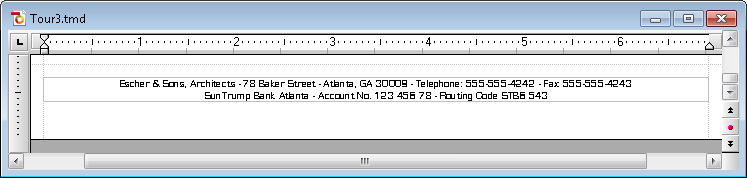
\includegraphics[scale=0.4]{00030.png}

Чтобы вернуться к обычному тексту после настройки колонтитула, просто нажмите мышью в любом месте текста. Если мы захотим изменить нижний колонтитул позже, всё, что нам нужно будет сделать, это нажать мышью на одной из строк колонтитула.

Пользуясь моментом, мы разместим завершающие письмо пожелания, под последней строкой письма. Введите пустую строку с помощью \keys{Enter} и напечатайте:

\begin{center}
\begin{tabular}{ | m{15cm} | }
\hline
С наилучшими пожеланиями,\keys{Enter}\\
\keys{Enter}\\
\keys{Enter}\\
\keys{Enter}\\
И.И.Сидоров,\keys{Enter}\\
ООО «Любовь и голуби»\keys{Enter}\\
\hline
\end{tabular}
\end{center}

На этом наше письмо в основном готово. В следующей и завершающей части урока мы разместим линию над нижним колонтитулом, чтобы выделить его получше.

\subsection{Линии и границы}
\textbf{\textit{Внимание}}: подробную информацию по этой теме можно найти в разделе \nameref{sec:границыилинии}.

В письме линия обычно размещается между нижним колонтитулом и основным текстом. Это очень легко сделать с помощью команды \textbf{Формат>Границы}. Её назначение — разместить границу вокруг абзаца или одиночные линии вдоль правого, левого,нижнего или верхнего края.

Чтобы разметить линию над нижним колонтитулом, нажмите на первую строку колонтитула и вызовите команду \textbf{Формат>Границы}.

Появится диалоговое окно, похожее на это:

\begin{figure}[ht]
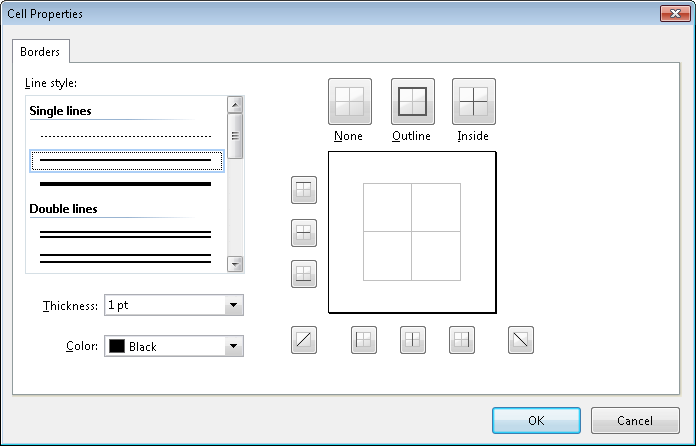
\includegraphics[scale=0.6]{00031.png}
\centering
\caption{Диалог границ}
\end{figure}

Как правило, работают с этим диалогом таким образом: сначала нужно указать какой тип линии нужен, а затем — где эту линию применить.

Соответственно, чтобы разместить линию над абзацем, нужно проделать следующее:
\begin{enumerate}
 \item Сначала выбираем тип линии, выбрав следующие параметры диалога:\\
\textbf{Стиль линии} (одиночная, двойная или пунктир)\\
\textbf{Толщина}\\
\textbf{Цвет}\\
В нашем примере мы укажем одиночную линию чёрного цвета толщиной 1пт.\\
Поскольку эти значения являются значениями по умолчанию, ничего в диалоге на этом этапе мы менять не будем.
\item Далее, укажем где применить эту линию (внизу, слева, справа и т.п.). Для этого в правой части диалога есть окошко предварительного просмотра с набором кнопок.\\
Чтобы применить границу, нажмите на соответствующую границу — прямо в окошке просмотра.\\
Или же можно добавить дополнительные линии, нажав на соответствующие границы в окошке просмотра, но нам сейчас нужна только одна.
\item Подтвердите, нажав на кнопку \textbf{OK}.
\end{enumerate}

Теперь абзац отделён тонкой чёрной линией.

Абзацы, набранные обычным текстом, можно оборудовать линиями, используя тот же самый способ, что мы применяли для колонтитулов. Кроме того, этот способ годится и для некоторых типов объектов — например, для ячеек таблицы.

\subsection{Печать письма-задания}
По желанию, вы можете теперь сделать пробную печать нашего первого сочинения. Для этого, вызовите команду \textbf{Файл>Печать} или нажмите сочетание клавиш \keys{Ctrl}+\keys{P}.

\begin{figure}[ht]
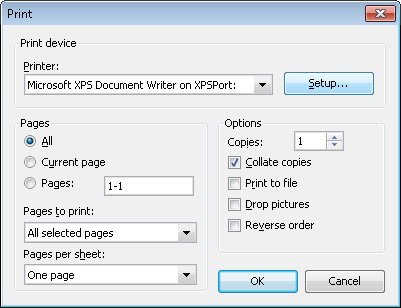
\includegraphics[scale=0.6]{00032.png}
\centering
\caption{Диалоговое окно \textbf{Файл>Печать}}
\end{figure}

В диалоговом окне «Печать» можно определить, сколько копий и каике именно страницы нужно распечатать. По умолчанию, печатается одна копия всех страниц. Подтвердите выбор с помощью кнопки OK. 

\textbf{Подсказка}: перед непосредственным процессом печати можно сделать предварительный просмотр с помощью команды \textbf{Файл>Предварительный просмотр}.

\subsection{Практическая работа закончена!}
Наш краткий обзор TextMaker в примерах на этом окончен. Пример окончательного документа можно найти в файле TOUR 4.TMD.

Теперь вы познакомились с базовым функционалом программы, и на этом этапе мы советуем уделить некоторое время дальнейшему изучению этих базовых функций. Хорошей практикой может стать, например, смена всего форматирования письма, смена шрифтов и т.д.

После этого можно углубиться в дальнейшее содержимое нашего Руководства. Руководство специально создано таким образом, чтобы пользователь мог изучить какую-то одну главу, посвящённую конкретной теме, нужной пользователю именно на текущем этапе работы. Таким образом, шаг за шагом, пользователь постигает весь функционал по мере возникающей необходимости.

Желаем продуктивной работы с TextMaker!

\section{Работа с выделениями} \label{sec:рсв}
Данная глава отмечает начало \textit{справочного раздела} нашего Руководства. Эта часть руководства предлагает подробное описание всех функций TextMaker, распределённых по тематическим главам, как это обычно и делается в справочных руководствах. 

Первая глава справочного руководства посвящена работе с \textit{выделениями}. Если нам нужно удалить, скопировать или переместить часть документа, эту часть необходимо сначала выделить. Это верно также и для объектов (рисунки, иллюстрации и т.д.).

Перед применением к тексту некоторых команд форматирования, текст необходимо также выделить. Например, для форматирования отдельного слова с помощью другого типа шрифта, это слово нужно выделить, перед тем, как устанавливать шрифт.

На последующих страницах рассказывается всё, что нужно знать при работе с выделениями. Включённые темы:

\begin{itemize}
 \item \textbf{Выделение текста и объектов}
 \item \textbf{Перемещение, удаление и копирование}
 \item \textbf{Вставка со специальным форматированием}
 \item \textbf{Вставка документов}
\end{itemize}

\subsection{Выделение текста и объектов} \label{sec:выделтекстаиобъект}
Перед выполнением команды TextMaker, во многих случаях нам нужно выделить фрагмент текста (или объект), к которому должна применяться команда. Далее команда применяется к этому выделенному тексту или объекту.

В зависимости от того, в какой ОС работает TextMaker, Windows/Linux или на устройстве Android, действия по выделению текста немного отличаются. Поэтому данный раздел разделён на две части:
\begin{itemize}
 \item Выделение в версии для Windows/Linux
 \item Выделение в версии для Android
\end{itemize}

\subsubsection{Выделение в версии для Windows/Linux}
В версии TextMaker для Windows и Linux выделять можно и с помощью мыши и с помощью клавиатуры:

\textbf{\textit{Выделение с помощью мыши}}

Выделения  с помощью мыши выполняется следующим образом:
\begin{itemize}
 \item \textbf{Выделение текста}\\
 Чтобы выделить \textit{фрагмент текста} любой длины, расположите курсор мыши в начале фрагмента, затем нажмите левую кнопку, и, не отпуская кнопки, протащите до конца фрагмента.\\
Чтобы выделить слово, сделайте двойной щелчок по слову.\\
Чтобы выделить целую строку, нажмите на левом поле рядом со строкой. Можно выделить несколько строк, протащив далее курсор мыши вверх или вниз по левому полю.\\
Чтобы выделить документ целиком, нажмите и удерживайте клавишу \keys{Ctrl}, а затем нажмите мышью по левому полю (рядом с любым абзацем документа).
\item \textbf{Выделение объектов}\\
Чтобы выделить объект (рисунок, картинку и т.д.), просто нажмите на него мышью. Вокруг объекта появится рамочка, обозначающая, что объект выделен.
\item \textbf{Отмена выделения}\\
Для отмены выделения просто нажмите мышью в любом месте документа за границами выделения.
\end{itemize}

\textbf{\textit{Выделение с помощью клавиатуры}}

\begin{itemize}
 \item \textbf{Выделение текста}\\
 Переместите текстовый курсор в начало фрагмента, который нужно выделить. Нажмите и удерживайте клавишу \keys{Shift}, и двигайте текстовый курсор в любом направлении с помощью клавиш со стрелками.
 
Мы можем выделить только один символ с помощью \keys{Shift}+\keys{\arrowkeyleft} или \keys{Shift}+\keys{\arrowkeyright}, или целые страницы с помощью \keys{Shift}+\keys{PgUp} или \keys{Shift}+\keys{PgDn}.

Чтобы выделить целый документ, соответственно используется сочетание клавиш \keys{Ctrl}+\keys{Home}, после которого следует сочетание клавиш \keys{Ctrl}+\keys{Shift}+\keys{End}. Тем не менее, для этого существует более быстрый способ: вызовите команду \textbf{Правка>Выделить всё}, или сочетание клавиш \keys{Ctrl}+\keys{A}.
\item \textbf{Выделение объектов}\\
Объекты можно выделять только с помощь мыши (см. выше).
\item \textbf{Отмена выделения}\\
Для отмены выделения достаточно нажать клавишу со стрелкой.
\end{itemize}

\textbf{\textit{Выделение в версии для Android}}
В версии для Android процедура выделения выглядит несколько иначе. Можно использовать либо палец либо мышь. Выполните следующее:
\begin{itemize}
 \item \textbf{Выделение текста}\\
Самый простой способ для выделения фрагмента текста следующий:\\
двойным касанием выделите слово, которое будет служить началом выделения. Перед и после слова появятся две «метки-манипулятора», обозначающие, что слово выделено.\\

\includegraphics[scale=0.6]{00033.png}\\
Эти две метки обозначают начало и конец выделения, и также дают возможность легко расширить выделение, просто протащив метки в нужных направлениях.
\item \textbf{Выделение объектов}\\
Чтобы выделить объект (картинку, рисунок и т.д.), коснитесь его. Вокруг объекта появится рамка, обозначающая, что объект выделен.
\item \textbf{Отмена выделения}\\
Для отмены выделения коснитесь документа вне границ выделения.
\end{itemize}

\subsection{Перемещение, удаление и копирование}
Во всех операционных системах, в которых работает TextMaker, имеется крайне удобный функционал: \textit{буфер обмена}.

Буфер обмена работает следующим образом: когда мы выделяем или вырезаем что-то из документа, этот фрагмент или объект попадает в буфер обмена. Объект временно помещается в буфер обмена для  того, чтобы его можно было далее повторно вставить в любом месте документа. Таким образом, буфер обмена облегчает удаление, копирование и перемещение фрагментов текста, а также и объектов.

Все необходимые команды находятся в меню «Правка»:

\begin{center}
\begin{longtable}{ | m{4cm} | m{10cm} | }
\hline
 \textbf{Команда} & \textbf{Объяснение} \\ 
 \hline
 Удалить & При выборе фрагмента текста и дальнейшем вызове команды \textbf{Правка>Удалить}, фрагмент или объект будет удалён — без помещения его в буфер обмена. Для более быстрого выполнения этого действия можно применять клавишу \keys{Delete}.\\
\hline
Вырезать & Команда \textbf{Правка>Вырезать} также удаляет содержимое выделения. Но не навсегда, а помещает содержимое выделения в буфер обмена, чтобы оно было доступно в любой момент позже для вставки в любом месте документа. Для вырезания также существует сочетание клавиш: \keys{Ctrl}+\keys{X}.\\
\hline
Копировать & Команда \textbf{Правка>Копировать} (сочетание клавиш \keys{Ctrl}+\keys{C}) копирует содержимое выделения в буфер обмена.\\
\hline
Вставить & Команда \textbf{Правка>Вставить} используется для вставки содержимого буфера обмена в текст. Переместите текстовый курсор на ту позицию в документе, где необходимо сделать вставку, и затем вызовите команду или нажмите \keys{Ctrl}+\keys{V}. Таким способом можно вставлять содержимое буфера обмена неоднократно.\\
\hline
\end{longtable}
\end{center}

В случае, если вам не до конца понятно, как буфер обмена помогает что-то удалять, копировать или перемещать, попробуйте рассмотреть всю процедуру с другой точки зрения:
\begin{itemize}
 \item \textbf{Как мне удалить текст?}\\
 Выделите фрагмент текста, и потом либо вырежьте его с помощью \keys{Ctrl}+\keys{X} для помещения его в буфер обмена, либо навсегда удалите его с помощью \keys{Delete}.
 \item \textbf{Как мне переместить текст?}\\
Выделите фрагмент текста и вырежьте его с помощью \keys{Ctrl}+\keys{X}. Потом переместите текстовый курсор на то место в тексте, куда необходимо переместить этот текст, и вставьте его с помощью \keys{Ctrl}+\keys{V}.
\item \textbf{Как мне скопировать текст?}\\
Выделите фрагмент текста и скопируйте его с помощью \keys{Ctrl}+\keys{C}. Потом переместите текстовый курсор на то место в тексте, куда необходимо скопировать этот фрагмент, и нажмите \keys{Ctrl}+\keys{V}.\\
Еси текст необходимо вставить снова, всё, что нужно сделать, это переместить курсор на следующую нужную позицию и снова нажать \keys{Ctrl}+\keys{V}.
\end{itemize}

Всё вышесказанное применимо и к объектам типа картинок и рисунков, как и способы, описанные ниже.

\subsection{Перемещение и копирование текста с помощью мыши (перетаскивание)}
Фрагмент текста, выделенный с помощью мыши, можно перетащить на другое место. С помощью этого способа, известного как «перетаскивание» (“drag and drop”), перемещение и копирование текста осуществляется очень быстро.

Выполните следующее:

\begin{enumerate}
 \item Выделите фрагмент текста.
 \item Расположите курсор мыши на выделении.
 \item Нажмите и не отпускайте левую копку мыши.
 \item С нажатой кнопкой мыши тащите выделение на необходимую позицию.
 \item После того, как вы отпустите кнопку мыши, содержимое выделения будет \textit{перемещено} в другое местоположение. А отпустив кнопку мыши при нажатой клавише \keys{Ctrl}, мы \textit{копируем} выделение в новое местоположение.
\end{enumerate}

\subsection{Вставка со специальным форматированием}
В дополнение к обычным операциям буфера обмена, таким, как \textbf{Вырезание}, \textbf{Копирование} и \textbf{Вставка}, TextMaker предлагает команду \textbf{Правка>Специальная вставка}, что даёт возможность лучше контролировать то, как именно содержимое вставляется в документ.

Подробнее:

Когда информация помещается в буфер обмена с помощью команд \textbf{Правка>Вырезать} или \textbf{Правка>Копировать}, то эта информация сохраняется в буфере в нескольких форматах. Например, если был скопирован текст, то этот текст сохраняется как в форматированном виде, так и не отформатированном виде.

Обычно это нас не волнует, т.к. TextMaker автоматически выбирает нужный формат во время вставки содержимого буфера обмена в документ по команде \textbf{Правка>Вставить}. Тем не менее, при необходимости можно выбрать формат, в котором содержимое будет вставлено. Для этого и существует команда \textbf{Правка>Специальная вставка}.

Во время вызова этой команды появляется диалоговое окно со списком всех форматов, в которых была сохранена информация, находящаяся на этот момент в буфере обмена. После выбора формата и подтверждения этого с помощи кнопки \textbf{OK}, содержимое буфера будет вставлено в выбранном формате.

\subsection{Вставка документов}
\begin{mdframed}[backgroundcolor=pink!50]
\textbf{\textit{FreeOffice}:} этот функционал отсутствует в \textbf{SoftMaker \textit{FreeOffice}}.
\end{mdframed}

С помощью команды \textbf{Вставить>Документ} можно в текущий документ вставить отдельный документ TextMaker.

Внимание: объекты с рамками (например, текстовый фрейм или текстовая рамка, фреймы рисунков и т.д.) \textit{не будут} импортированы.

Выполните следующее:
\begin{enumerate}
 \item Переместите текстовый курсор на ту позицию в документе, куда необходимо вставить другой документ.
 \item Вызовите команду \textbf{Вставка>Документ}.
 \item Будет открыто диалоговое окно, в котором можно выбрать документ для импорта.
 \item Подведите выбор с помощью кнопки OK.
\end{enumerate}

Выбранный документ будет вставлен.

\section{Форматирование символов} \label{sec:фс}
С помощью команды \textbf{Формат>Шрифт} можно изменить внешний вид одного или более символов в документе.

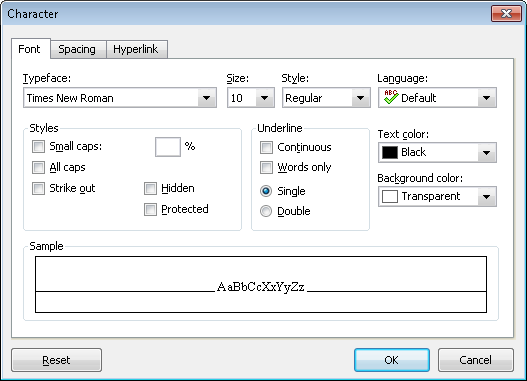
\includegraphics[scale=0.6]{00017.png}

Параметры в диалоге \textbf{Формат>Шрифт} распределены по нескольким вкладкам, перемещаться между которыми можно с помощью нажатий мыши.
\begin{itemize}
 \item Вкладка \textbf{Шрифт}\\
Используется для выбора гарнитуры и размера шрифта, стилей (полужирный, курсив и подчёркнутый), цветов текста и языка.
\item Вкладка \textbf{Интервал}\\
Используется для изменения таких свойств, как надстрочный/подстрочный формат, межсимвольный интервал, шаг печати и кернинг.
\item Вкладка \textbf{Гиперссылка}\\
Используется для вставки и редактирования гиперссылок (т.е. веб-страниц). Информацию по этой теме можно найти в разделе \nameref{sec:создссылок}.
\end{itemize}

\textbf{Изменение формата символов}\\
Существует два способа изменить формат символов:
\begin{itemize}
 \item \textit{После того, как был введён текст}, его можно изменить, выделив нужный текст, вызвав команду \textbf{Формат>Шрифт} и внеся необходимые изменения.
 \item \textit{По мере ввода текста}, его можно изменять, вызывая команду \textbf{Формат>Шрифт}, и продолжая печать далее. С момента, например, выбора другого шрифта, вводимый текст будет форматирован этим шрифтом, до того момента, когда его снова понадобится изменить.
\end{itemize}

Дополнительная информация по теме форматирования символов представлена на следующих страницах.

\subsection{Гарнитура и размер шрифта}
Чтобы изменить гарнитуру и/или размер шрифта, сделайте следующее:
\begin{enumerate}
 \item Выделите текст, который нужно изменить.
\item Вызовите команду \textbf{Формат>Шрифт}.
\item Перейдите на вкладку \textbf{Шрифт}.
\end{enumerate}

Теперь можно установить нужную гарнитуру и размер шрифта:
\begin{itemize}
 \item Чтобы изменить гарнитуру, откройте выпадающий список «Гарнитура», нажав на маленькую стрелку справа, и выберите нужную.
 \item Наиболее часто употребляемые размеры шрифтов представлены в списке выпадающего меню «Размер». Можно выбрать один из представленных размеров или же вести другой размер вручную, при этом возможно указать и десятые доли размера, например, 12,7 пт.
\end{itemize}

Размеры шрифта традиционно указываются в пунктах (пт). Как правило, для основного текста используют размеры между 10 и 12 пт, и от 14 до 18 для заголовков. Основные заголовки могут быть ещё больше (например , 24пт).

\subsubsection{Работа с панелью Форматирования}
Гарнитуру и размер шрифта также можно изменить с помощью панели Форматирования.

\begin{figure}[ht]

\includegraphics[scale=0.6]{00013.png}
\centering
\caption{Панель форматирования}
\end{figure}

Для этого нужно выделить текст, открыть выпадающий список с гарнитурами или с размерами шрифтов и выбрать желаемые значения нажатием кнопки мыши.

\subsection{Стили шрифта}
Стили шрифта — это такие параметры выделения текста, как полужирный шрифт, курсив, подчёркнутый и т.п. 

TextMaker представляет следующие стили текста:
\begin{itemize}
 \item \textit{Курсив} — гарнитура с наклоном
 \item \textbf{Полужирный} — утолщённая гарнитура
 \item \textsc{Малые прописные (капители)} — строчные буквы заменяются малыми прописными
 \item ПРОПИСНЫЕ — все буквы являются заглавными
 \item \sout{Перечёркнутые} — текст перечёркнут
 \item Скрытый — текст не выводится на экран, не выводится на печать или не показывается обоих случаях (см. раздел \nameref{sec:скрытыйтекст})
 \item Защищённый — текст не подлежит изменению (см. раздел \nameref{sec:защитатекста})
 \item \underline{Подчёркнутый} — одинарное или двойное подчёркивание текста. Линия может быть непрерывной или подчёркивать только слова.
 \item Надстрочный (например, x\textsuperscript{2}) или подстрочный (H\textsubscript{2}O) — эти стили можно найти в следующей вкладке (см. раздел \nameref{sec:надстриподстршрифты})
 \item Цвет текста и цвет фона — см. следующий раздел
 \item Язык — при необходимости можно также указать язык для фрагмента текста (это требуется, только если в документе используется больше одного языка, см. раздел \nameref{sec:языксредства})
\end{itemize}

\subsubsection{Применение стилей к тексту}
Чтобы применить стиль к тексту, вызовите команду \textbf{Формат>Шрифт} и переключитесь на вкладку \textbf{Шрифт}.

Чтобы включить полужирный или курсив, откройте выпадающий список \textbf{Стиль} (справа от выбора размера) и выберите нужный стиль из списка: Обычный, \textit{Курсив}, \textbf{Полужирный} или \textit{\textbf{Полужирный курсив}}.

Чтобы применить другие стили, включите или отключите их, отметив галочкой соответствующие параметры в диалоге \textbf{Стили}.

Пользователь не ограничен только одним стилем, можно применять сочетания стилей, хотя не все сочетания возможны.

\subsubsection{Использование панели Форматирования}


\includegraphics[scale=0.6]{00035.png}

Нажмите на значок того стиля, который нужно применить или отменить: \textbf{B} — полужирный, \textit{I} — курсив, \underline{U} — непрерывное подчёркивание.

\begin{mdframed}[backgroundcolor=blue!10]
\textbf{Совет:} для применения этих стилей также существуют сочетания клавиш: \keys{Ctrl}+\keys{B}, \keys{Ctrl}+\keys{I} и \keys{Ctrl}+\keys{U}, соответственно.
\end{mdframed}

\subsection{Цвет текста}
Можно указывать цвет как для текста, так и для его фона.

Для этого:
\begin{enumerate}
 \item Выделите нужный текст.
 \item Вызовите команду \textbf{Формат>Шрифт}
 \item Перейдите на вкладку Шрифт.
\end{enumerate}

Теперь можно выбрать желаемый цвет текста из списка \textbf{Цвет текста}.

Также можно указать цвет фона в списке \textbf{Цвет фона}. По умолчанию, фон для текста является прозрачным. Если указать цвет для фона, то эффект текста на цветном фоне будет аналогичным эффекту цветного маркера на бумаге.

\subsubsection{Примечания}
\begin{itemize}
 \item Цвет текста по умолчанию с названием «Автоматический» имеет особенное свойство: текст, форматированный в этом цвете, обычно показывается чёрным. Тем не менее, если изменить цвет фона на какой-нибудь очень тёмный цвет, цвет текста автоматически сменится на белый (чтобы сохранить читаемость текста).
 \item Если никакой из предложенных в списке цветов не устраивает пользователя, всегда можно создать свой цвет. Для этого нажмите на кнопку «Задать цвет» (последний пункт в списке цветов). См. также раздел \nameref{sec:свойствадоквклцвета}.
 \item Цвет текста также можно изменять с помощью списка цветов 
\includegraphics[scale=0.6]{00036.png} на панели \textbf{Форматирования}. Нажмите на этот список (в правой части панели) и выберите нужный цвет.
 \item Непосредственно справа от цвета текста находится элемент для Выделения цветом, также в виде раскрывающегося списка. С его помощью можно добавить цвет \textit{выделения} для выбранного теста, по аналогии с выделением цветным маркером.\\
 Внимание: эта возможность \textit{не} является аналогичной цвету фона, описанному выше. Это — \textit{дополнительный} цвет, который можно применить только с помощью данного выпадающего писка на панели. Логику этого функционала можно оспаривать, но именно в таком виде он присутствует в Microsoft Word, поэтому в TextMaker он реализован точно так же, в интересах совместимости.
\end{itemize}

\subsection{Надстрочный и подстрочный шрифты} \label{sec:надстриподстршрифты}
Расположение шрифта выше (x\textsuperscript{2}) или ниже (H\textsubscript{2}O) базовой линии шрифта называется надстрочным или подстрочным написанием (или верхним или нижним индексом).

Выделите текст, вызовите команду \textbf{Формат>Шрифт}, перейдите на вкладку \textbf{Интервал}, и отметьте галочкой параметр «Надстрочный» или «Подстрочный».

При желании, можно указать размер сдвига ниже или выше базовой линии, введя процентное значение в окошке «Позиция». Кроме того, можно указать точное процентное уменьшение размера надстрочного/подстрочного шрифта в окошке «Размер». Если, например, пользователю необходимо, чтобы размер  надстрочного/подстрочного шрифта соответствовал размеру нормального текста, то нужно отметить 100\%.

\textbf{\textit{Совет}}: для установки надстрочного и подстрочного шрифта доступны также следующие сочетания клавиш: \keys{Ctrl}\keys{Shift}\keys{NumLock} (клавиша плюс, расположенная на вспомогательной цифровой клавиатуре) для надстрочного шрифта, \keys{Ctrl}\keys{Shift}\keys{NumLock\textminus} для подстрочного, \keys{Ctrl}\keys{Shift}\keys{NumLock*} — для удаления либо того либо другого.

\subsection{Межсимвольный интервал и плотность расположения знаков}
TextMaker также даёт возможность изменять межсимвольный интервал и плотность расположения знаков.

Интервал — это расстояние по горизонтали между символами. Значение меньше 100\% приближает символы друг к другу; значение больше 100\% — отдаляет.
Параметр «плотность расположения» влияет на ширину букв шрифта, а не на расстояние между ними.

Для изменения этих параметров вызовите \textbf{Формат>Шрифт}, перейдите на вкладку \textbf{Интервал} и введите нужное значение в поле \textbf{Межсимвольный интервал} или \textbf{Плотность расположения}.

\textit{\textbf{Внимание}}: изменение плотности расположения для \textit{внутренних} шрифтов некоторых принтеров игнорируется на выводе печати.

\subsection{Кернинг}
Некоторые пары букв выглядят лучше, если интервал между ними немного уменьшить или немного увеличить. Такое действие, называемое «кернинг», в TextMaker можно выполнять автоматически.

С помощью этой иллюстрации можно лучше понять, что такое кернинг:

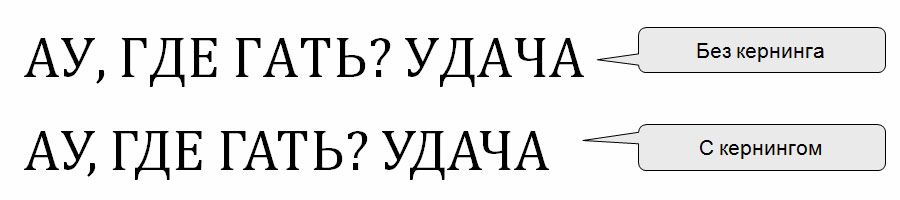
\includegraphics[scale=0.3]{00037.png}

Чтобы включить кернинг, выберите нужный текст, выберите команду \textbf{Формат>Шрифт}, перейдите на вкладку \textbf{Интервал} и активируйте параметр \textbf{Использовать кернинг}.

С этого момента TextMaker автоматически будет настраивать интервалы между буквами там, где это улучшит внешний вид текста.

\textit{\textbf{Внимание}}: не все гарнитуры предоставляют \textit{информацию о кернинге} в данных шрифтов, нужную для программного определения того, какие именно пары букв нужно настраивать, и как. Почти все наборы шрифтов, опубликованные \textbf{SoftMaker}, включают в себя исчерпывающую информацию о кернинге.

\subsection{Перенос форматирования}

\begin{mdframed}[backgroundcolor=pink!50]
\textbf{\textit{FreeOffice}:} этот функционал отсутствует в \textbf{SoftMaker \textit{FreeOffice}}.
\end{mdframed}

С помощью команды \textbf{Формат>Перенести форматирование} можно быстро применить формат шрифта (гарнитура, размер, стиль и др) к другим символам.

Для этого сделайте следующее:
\begin{enumerate}
 \item Выберите символ, формат которого нужно изменить. Можно также выбрать несколько символов, но их формат должен быть одинаковый.
 \item Вызовите команду \textbf{Формат>Перенести форматирование}.\\
Курсор мыши примет форму маленькой кисти: 
\includegraphics[scale=1]{00038.png}
\item Удерживая левую кнопку, протащите мышь по символам, формат которых нужно перенести.\\
\textit{\textbf{Совет}}: если вышеуказанное действие проделать при нажатой клавише \keys{Ctrl}, то будет перенесён не только формат символов, но и формат абзаца.
\item Если необходимо перенести форматирование неоднократно, повторите шаг 3 столько раз, сколько это нужно.
\item Закончив, снова вызовите команду \textbf{Формат>Перенести форматирование} или просто нажмите клавишу Esc.
\end{enumerate}

\subsection{Скрытый текст} \label{sec:скрытыйтекст}
TextMaker даёт возможность скрывать текст. Обычно, скрытый текст показывается на экране, но не выводится на печать.

Скрытый текст идеально подходит для комментариев или примечаний, которые необходимы в тексте, но не нужны в печатном варианте документа.

\subsubsection{Скрытие текста}
Чтобы скрыть текст, проделайте следующее:
\begin{enumerate}
 \item Выделите текст, который необходимо скрыть.
 \item Вызовите команду \textbf{Формат>Шрифт}.
 \item Отметьте параметр «Скрытый».
\end{enumerate}

Теперь текст является скрытым. По умолчанию, он будет показываться на экране, но будет отсутствовать при печати документа.

\subsubsection{Показ/печать скрытого текста}
По умолчанию, скрытый текст виден на экране, но не показывается на отпечатанной странице. Тем не менее, в свойствах документа можно указать, нужно ли показывать скрытый текст на экране, и нужно ли скрытый текст печатать.

Для этого, вызовите команду \textbf{Файл>Свойства} и переключитесь на вкладку \textbf{Вид}. В разделе «Скрытый текст» присутствуют следующие параметры:
\begin{itemize}
 \item \textbf{Показать скрытый текст}\\
Этот параметр контролирует видимость скрытого текста на экране.\\
Этот параметр отмечен по умолчанию, и по умолчанию скрытый текст виден на экране. Скрытый текст выделяется нижним подчёркиванием в виде точек, так чтобы его можно было отличить от обычного текста.\\
Если отключить этот параметр, скрытый текст не будет виден на экране.
\item \textbf{Печатать скрытый текст}

Параметр \textbf{Печатать скрытый текст} контролирует вывод скрытого текста на печать вместе с обычным текстом.\\
По умолчанию, этот параметр не отмечен, и скрытый текст отсутствует в отпечатанном документе.\\
Этот параметр нужно отметить, если необходимо вывести скрытый текст на печать.
\end{itemize}

\subsubsection{Удаление свойства «скрытый»}
Если пользователю необходимо удалить форматирование текста как «скрытого», нужно сделать следующее:
\begin{enumerate}
 \item Убедитесь, что параметр «показать скрытый текст» отмечен в свойствах документа (см. выше), так что скрытый текст виден при просмотре документа на экране.
 \item Выделите скрытый текст, вызовите команду \textbf{Формат>Шрифт} и снимите галочку с параметра «Скрытый» во вкладке \textbf{Шрифт}.
\end{enumerate}
Текст  более не является скрытым.

\subsection{Защита текста} \label{sec:защитатекста}
Фрагмент текста можно защитить от изменений или удаления.
\subsubsection{Защита текста}
Чтобы защитить текст, выполните следующее:
\begin{enumerate}
 \item Выделите текст, который нужно защитить.
 \item Вызовите команду \textbf{Формат>Шрифт}.
 \item Переключитесь на вкладку \textbf{Шрифт}.
 \item Отметьте параметр \textbf{Защищённый}.
\end{enumerate}
Текст, защищённый таким образом, нельзя изменять. Если поместить текстовый курсор в такой текст и попытаться что-то напечатать или удалить, эти действия не будут иметь никакого эффекта.

\begin{mdframed}[backgroundcolor=blue!10]
\textbf{\textit{Важное примечание:}} если выделить фрагмент текста, включающий в себя скрытый текст, и удалить этот фрагмент, то защищённый текст, входящий в этот фрагмент, будет удалён вместе с обычным текстом. Защита предотвращает редактирование или удаление только в границах скрытого текста.
\end{mdframed}

\subsubsection{Удаление свойства «защищённый»} 
Чтобы удалить защиту с текста, выделите нужный фрагмент защищённого текста, вызовите команду \textbf{Формат>Шрифт} и снимите галочку с параметра \textbf{Защищённый} во вкладке \textbf{Шрифт}.

Фрагмент текста более не защищён, и его можно удалять и редактировать.

\textbf{Удаление форматирования}

В случае, если необходимо удалить форматирование символов, в TextMaker это можно сделать быстро и просто.

Выполните следующие действия:
\begin{enumerate}
 \item Выделите нужный фрагмент текста.
 \item Вызовите команду \textbf{Формат>Стандартный} или нажмите сочетание клавиш \keys{Ctrl}+\keys{Пробел}.
\end{enumerate}

TextMaker удалит любое форматирование, ранее применённое к тексту с помощью команды \textbf{Формат>Шрифт} или с помощью панели \textbf{Форматирования}.

Форматирование абзаца и форматирование символов, являющихся стиля абзаца, останется нетронутым.

\begin{mdframed}[backgroundcolor=blue!10]
\textbf{Внимание:} это действие также удаляет свойства текста \textbf{Скрытый} и \textbf{Защищённый}. Соответственно, ранее скрытый текст станет видимым, а ранее защищённый текст станет возможно редактировать.
\end{mdframed}

\subsection{Изменение форматирования по умолчанию}
Стандартное форматирование можно изменить в любое время. Если, например, пользователю не нравится выбранный по умолчанию шрифт, то это можно изменить за несколько нажатий мыши.

Выполните следующее:
\begin{enumerate}
 \item Вызовите команду \textbf{Формат>Шрифт}.
 \item В диалоговом окне настройте желаемые параметры по своему выбору.
 \item Теперь внимание: вместо нажатия на кнопку OK, нажмите на кнопку \textbf{Установить по умолчанию}.
 \item TextMaker выведет запрос, нужно ли изменить параметры по умолчанию только для текущего документа или также и для всех последующих документов.\\
\textbf{Изменить только в этом документе:} при выборе этого параметра, изменённое форматирование по умолчанию будет применено только к текущему документу.\\
\textbf{Изменить для всех новых документов:} при выборе этого параметра, изменённое форматирование по умолчанию будет сохранено в стандартном шаблоне документа (Normal.tmv), и, соответственно, все будущие документы будут созданы на основе этих параметров.
\item Подтвердите выбор с помощью кнопки \textbf{OK}.
\item Для выхода из диалога снова нажмите \textbf{OK}.
\end{enumerate}

TextMaker сохранит выбранные параметры форматирования в качестве параметров по умолчанию.

(Для продвинутых пользователей: с технической точки зрения, TextMaker просто применяет эти параметры к стилю по умолчанию  «Обычный». См. также раздел \nameref{sec:стильсимволовобычный}.)

\section{Форматирование абзацев} \label{sec:фа}
Чтобы установить форматы для абзацев, используйте команду \textbf{Формат>Абзац}.

Вот наиболее часто используемые параметры для формата абзацев:
\begin{itemize}
 \item Отступы
 \item Интервал между строками
 \item Интервал над/под абзацем
 \item Выравнивание абзацев
 \item Формат символов для всего абзаца
 \item Табуляция
\end{itemize}

Также доступны следующие дополнительные параметры:
\begin{enumerate}
 \item Маркированный список (и нумерованный список)
 \item Буквица
 \item Заливка
 \item Границы и линии
 \item Уровень разбивки
 \item Частота переносов (см. раздел «Переносы»)
 \item Принудительная разбивка перед абзацами (разрыв страницы, разрыв колонки)
 \item Контроль абзацев (не отрывать абзац от следующего и т.п.)
 \item Подавление нумерации строк
\end{enumerate}

Подробности см. далее.

Форматирование абзацев всегда применяется только к абзацам целиком. Изменения форматирования абзаца влияет на весь абзац, в котором расположен текстовый курсор. При выборе нескольких абзацев, форматирование меняется во всех выбранных абзацах.

\textbf{Изменение форматирования абзацев}

Изменить форматирование абзацев можно одним из следующих способов:
\begin{itemize}
 \item Чтобы изменить форматирование абзацев после того, как они были напечатаны, выберите нужный абзац, вызовите команду \textbf{Формат>Абзац} и сделайте необходимые изменения.
 \item Чтобы изменить форматирование абзацев во время их набора, установите нужное форматирование с помощью команды \textbf{Формат>Абзац}, без выделения. Текущий абзац будет переформатирован согласно новым параметрам. Далее эти параметры будут применяться ко всем новым абзацам, начинаемым по нажатию клавиши \textbf{Enter}, до тех пор, пока пользователь снова не изменит форматирование.
\end{itemize}

\textbf{Стили абзаца (для продвинутых пользователей):} стили абзаца — это способ значительно сократить общий объём работы при форматировании абзацев. С их помощью можно очень быстро применить предварительно настроенные форматы. Эту информацию можно найти в главе \nameref{sec:стили}.

Единицы измерения: значения в диалоговых окошках TextMaker можно вводить в различных единицах.

\begin{center}
\begin{tabular}{ | m{4cm} | m{4cm} | }
\hline
 \textbf{Единица измерения} & \textbf{Объяснение} \\ 
 \hline
 см & Сантиметры\\
\hline
... & Дюймы\\
\hline
пт & Пункты \\
\hline
пи & Пики\\
\hline
\end{tabular}
\end{center}

\subsection{Отступы} \label{sec:отступы}
С помощью отступов мы изменяем правые и левые границы абзацев для сужения или расширения текста. Отступ для первой строки абзаца можно настроить отдельно.
Отступы всегда указываются относительно полей страницы. Если, например, левое поле страницы настроено на 1 см, и \textbf{Левый} отступ настроен на 1,5см, то текст будет начинаться на расстоянии в 2,5см.

\begin{mdframed}[backgroundcolor=blue!10]
\textbf{Внимание:} поля страницы указываются с помощью команды \textbf{Файл>Параметры страницы}, а \textit{не} с помощью отступов.
\end{mdframed}

Чтобы использовать отступы, поместите курсор внутрь нужного абзаца или выберите несколько абзацев. Затем вызовите команду \textbf{Формат>Абзац} и перейдите на вкладку \textbf{Абзац}.

В диалоговом поле «Отступы»  можно указать Левый отступ, Правый отступ и отступ для Первой строки. Введите нужные значение в соответствующие окошки.
Если, например, нам нужно расширить текст, то можно ввести отрицательное значение.

\subsubsection{Использование горизонтальной линейки}
Включенная горизонтальная линейка (отмеченный параметр \textbf{Вид>Горизонтальная линейка}) предоставляет удобный альтернативный способ для изменения отступов.

Отступы показывается на линейке следующим образом:

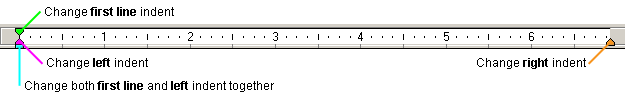
\includegraphics[scale=0.8]{00039.png}

Чтобы изменить отступ, сначала выберите абзац(ы), который нужно изменить, далее нажмите мышью на один из треугольных манипуляторов на линейке (см. картинку выше), и удерживая кнопку мыши, перетащите его на нужную позицию.

Изменяя \textbf{Левый} отступ, внимательно выбирайте нужный треугольник — за левый отступ отвечает \textit{нижний} треугольник. Соответственно, \textit{верхний} манипулятор-треугольник отвечает за отступ только для \textbf{Первой} строки. \textit{Прямоугольный} манипулятор отвечает за изменение \textbf{Правого и Левого} отступов \textit{одновременно}.

\subsubsection{С использованием клавиатуры}
Отступы также можно изменять с помощью следующих сочетаний клавиш:
\begin{itemize}
 \item Увеличить \textbf{Левый} отступ: \keys{Ctrl}+\keys{M}
 \item Уменьшить \textbf{Левый} отступ: \keys{Ctrl}+\keys{Shift}+\keys{M}
 \item Увеличить висячий отступ*: \keys{Ctrl}+\keys{T} 
\end{itemize}

* Увеличивает \textbf{Левый} отступ, одновременно уменьшая отступ \textbf{Первой} строки. В итоге, первая строка абзаца сохраняет свою позицию, а отступ применяется к другим строкам.

\subsection{Межстрочный интервал}
Интервал между строками (межстрочный интервал) — это расстояние между строками в абзаце. 

Чтобы изменить интервал между строками, сделайте следующее:
\begin{enumerate}
 \item Поместите текстовый курсор в нужный абзац (или выделите несколько абзацев).
 \item Вызовите команду \textbf{Формат>Абзац}.
 \item Переключитесь на вкладку «Абзац».\\
 Параметры интервалов находятся в блоке «Межстрочный интервал»:
 \item Сначала нужно выбрать способ указания межстрочного интервала (см. ниже) в выпадающем списке.
 \item Затем введите интервал в блоке редактирования справа.
\end{enumerate}

После подтверждения параметров с помощью кнопки \textbf{OK}, межстрочный интервал будет изменён.

\subsubsection{Способы указания межстрочного интервала}
Есть несколько способов указания межстрочных интервалов. В выпадающем списке «Межстрочный интервал» можно выбрать один из следующих способов:
\begin{itemize}
 \item \textbf{Одинарный}\\
 Автоматический одинарный межстрочный интервал.\\
Определяет оптимальный интервал \textit{автоматически}:\\
При увеличении размера шрифта абзаца,  межстрочный интервал увеличивается автоматически.\\
При уменьшении размера шрифта, интервал уменьшается соответственно.
\item \textbf{Множественный}\\
Несколько автоматических одинарных межстрочных интервалов.\\
Точно так же, как и параметр \textbf{Одинарный}, этот параметр определяет оптимальный интервал автоматически. Тем не менее, при необходимости, межстрочный интервал можно легко увеличить или уменьшить. Для этого нужно просто ввести нужное число строк в блок редактирования справа.

Несколько примеров:\\
Если в блок редактирования ввести значение «1.5», то автоматически определяемый интервал будет умножен на 1,5 (что даёт полтора автоматических интервала).
При вводе значения «2» автоматически определяемый интервал умножается на 2 (что даёт двойной автоматический интервал).
Значение «1» соответствует выбору параметра \textbf{Одинарный} (что даёт автоматический одинарный интервал).
\item \textbf{Точно}\\
Фиксированный межстрочный интервал.\\
Этот параметр даёт возможность указать \textit{точное} значение интервала вручную, в пунктах. В этом случае интервал \textit{не} будет согласовываться с размером шрифта.

\textbf{Подсказка}: проверенным практическим размером для корректного межстрочного интервала является формула Межстрочный интервал = Размер шрифта x 1,2
Так, для шрифта размером в 10пт советуется применять межстрочный интервал в 12пт.
\item \textbf{Не менее}\\
Автоматический межстрочный интервал с указанным минимальным значением.
Так же, как и параметр \textbf{Одинарный}, этот параметр предоставляет автоматический одинарный интервал — но препятствует его уменьшению ниже указанного минимального значения.

Так, если для минимального значения ввести значение в 12пт, то будет применяться автоматический одинарный интервал. Но если автоматический одинарный межстрочный интервал примет значение меньше 12 пт (например, при использовании очень маленького размера шрифта), то вместо этого будет применяться фиксированный интервал в 12пт.
\end{itemize}

По умолчанию для межстрочного интервала указано значение \textbf{Одинарный}.

Для наиболее часто употребляемых значений также существуют сочетания клавиш:

\keys{Ctrl}+\keys{1} — автоматический одинарный интервал (1 строка)

\keys{Ctrl}+\keys{5} — автоматический полуторный интервал (1,5 строки)

\keys{Ctrl}+\keys{2} — автоматический двойной межстрочный интервал (2 строки)

\subsection{Интервал между абзацами}
Кроме межстрочного интервала, можно также указать количество пустого пространства, добавляемого над первой строкой и ниже последней строки абзаца.  
Чтобы изменить эти параметры, вызовите команду \textbf{Формат>Абзац} и перейдите на вкладку \textbf{Абзац}.

В групповом блоке \textbf{Интервал} между абзацами доступны следующие возможности: 

\subsubsection{Перед}
Здесь можно указать объём пустого пространства между окончанием предыдущего абзаца и началом текущего. 

\subsubsection{После}
Здесь указывается объём пустого пространства между окончанием текущего абзаца и началом следующего. 

\subsubsection{Подавить для абзацев с одинаковым стилем абзаца}
Этот параметр был введён в основном для поддержки совместимости с Microsoft Word. Включение его включит следующие свойства:
\begin{itemize}
 \item Если текущий и предыдущий абзацы используют один и тот же стиль абзаца, интервал «перед» применяться не будет.
 \item Если текущий и следующий абзацы используют один и тот же стиль абзаца, интервал «После» применяться не будет.
 \end{itemize}
 
 По умолчанию, этот параметр отключен.
 
 \subsection{Выравнивание абзацев}
 Способ, каким TextMaker организует текстовые абзацы, называется «выравнивание абзацев». В TextMaker существует четыре типа выравнивания абзацев:
 \begin{itemize}
  \item Влево \keys{Ctrl}+\keys{L}
  \item Вправо \keys{Ctrl}+\keys{R}
  \item По центру \keys{Ctrl}+\keys{E}
  \item \keys{Ctrl}+\keys{J}
 \end{itemize}

Чтобы изменить выравнивание абзацев, выделите необходимые абзацы и нажмите одно из указанных выше сочетаний клавиш.

Или можно вызвать команду \textbf{Формат>Абзац}, перейти на вкладку \textbf{Абзац} и выбрать способ выравнивания в выпадающем списке «Выравнивание».

\subsubsection{С помощью панели Форматирования}
Для изменения выравнивания можно также использовать панель \textbf{Форматирования}. Для этого, нажмите на одну из следующих кнопок:


\includegraphics[scale=0.6]{00018.png} Выравнивать абзац влево


\includegraphics[scale=0.6]{00019.png} Выравнивать абзац вправо


\includegraphics[scale=0.6]{00020.png} Выравнивать абзац по центру


\includegraphics[scale=0.6]{00021.png} Выравнивать абзац по ширине страницы

Выравнивание абзаца изменится соответственно.

\subsubsection{Изменение направления текста}

Для текста, написанного арабским письмом, существует дополнительная возможность под названием «Направление текста» , с помощью которой можно установить направление письма в абзаце справа налево. Также см. главу \nameref{sec:работастекстнаараб}.

\subsection{Формат символов для абзацев целиком}
В диалоговом окне команды \textbf{Формат>Абзац}, во вкладке \textbf{Абзац} также можно увидеть кнопку \textbf{Шрифт}. С её помощью можно изменить форматирование символов (шрифт, стили текста и т.д.) для абзацев целиком. Это особенно удобно для стилей абзаца (см. раздел \nameref{sec:стилиабзаца}).

Чтобы изменить форматирование символов для для целых абзацев, выделите нужный абзац, вызовите команду \textbf{Формат>Абзац} и нажмите на эту кнопку. Будет показано диалоговое окно, в котором можно настроить желаемый формат для символов (см. раздел \nameref{sec:фс}).

\subsection{Табуляция} \label{sec:табуляция}
Шаг табуляции — это «прыжок», с помощью которого мы позиционируем текстовый курсор в конкретной точке строки. Табуляция помогает, например, составлять, табличные отчёты. 

Чтобы начать работать с табуляциями необходимо сделать два шага:
\begin{enumerate}
 \item Определить шаг табуляции с помощью команды \textbf{Формат>Табуляции}. Эта команда используется для указания позиций, на которые табуляция передвинет курсор.
 \item С помощью клавиши \keys{Tab} передвинуть текстовый курсор от одного шага к другому — это называется «ввод табуляции».
\end{enumerate}

\textbf{Внимание}: хотя на большинстве клавиатур клавишу табуляции помечена значком \keys{Tab} , в нашем руководстве мы используем обозначение \keys{Tab}, чтобы  пользователь не спутал его со значками клавиш со стрелками.

Подробности о работе с табуляциями см. ниже.

\subsubsection{Использование табуляции}
По умолчанию, шаг табуляции равен интервалу примерно в 1,25 см (0,5 дюйма). Но это значение осталось ещё с эры печатных машинок, и пользователь ни в коем случае им не ограничен.

Для каждого абзаца документа можно настроить свой шаг табуляции.

Чтобы настроить шаги табуляции, выполните следующее:
\begin{enumerate}
 \item Расположите текстовый курсор в нужном абзаце (или выберите несколько абзацев).
 \item Вызовите команду \textbf{Формат>Табуляции}.\\
 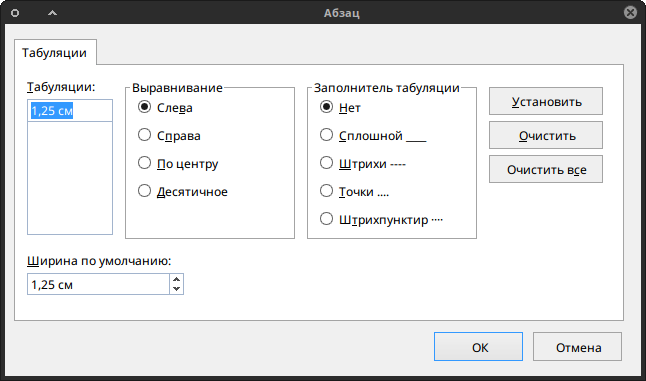
\includegraphics[scale=0.6]{00040.png}
 \item В диалоговом окне \textbf{Табуляции} введите желаемое значение для позиции относительно левой границы страницы, где значение «0» соответствует непосредственно левой границы страницы.
 \item При желании, выберите другое \textbf{Выравнивание} и другой \textbf{Заполнитель} табуляции для шага табуляции (см. ниже).
 \item \textit{Не забудьте} нажать на кнопку \textbf{Установить}.
 \item При необходимости, точно также настройте дополнительные шаги табуляции, и завершите работу в диалоговом окне нажатием кнопки \textbf{OK}.
\end{enumerate}

После настройки шагов табуляции, с помощью клавиши \keys{Tab} их можно вставлять в документ.

\textbf{Внимание}: этот диалог можно также использовать для указания \textbf{Стандартной ширины} для предварительно настроенных шагов табуляции, о которых мы упоминали ранее. Но после установки пользовательских шагов табуляции для конкретного абзаца, предварительно настроенные стандартные шаги игнорируются.

\subsubsection{Выравнивание табуляции}
С помощью команды \textbf{Формат>Табуляции} можно установить не только позицию для нового шага, но также и его выравнивание:

\begin{center}
\begin{tabular}{ | m{4cm} | m{10cm} | }
\hline
 \textbf{Выравнивание} & \textbf{Эффект} \\ 
 \hline
 Слева & Обычный шаг табуляции аналогичный шагу пишущей машинки. Шаг табуляции отмечает место, с которого \textit{начинается} текст.\\
\hline
Справа & Текст после шага табуляции выравнивается по правому краю. Шаг табуляции отмечает место, где текст \textit{заканчивается}.\\
\hline
По центру & Текст, вводимый после шага табуляции, центрируется по позиции табуляции. Шаг табуляции отмечает \textit{середину} вводимого текста.\\
\hline
Десятичное & Для форматирования цифровых столбцов. Цифры располагаются таким образом, чтобы \textit{десятичные разделители} были выравнены по вертикали.\\
\hline
\end{tabular}
\end{center}

\textbf{Совет}: чтобы изменить выравнивание уже существующего шага табуляции, вызовите команду \textbf{Формат>Табуляции}. Выберите один из  настроенных шагов табуляции, измените его выравнивание и нажмите на кнопку \textbf{«Установить»}.

\subsubsection{Заполнитель табуляции}
При желании, пространство шага табуляции можно заполнить следующими символами заполнения:

\begin{center}
\begin{tabular}{ | m{3cm} | m{3cm} | m{7cm} |}
\hline
 Нет &  & Табуляция без заполнения\\ 
 \hline
Сплошной &  & Заполнение сплошным подчеркиванием\\
\hline
Штрихи & \Kutline\Kutline\Kutline\Kutline\Kutline\Kutline & Заполнение штрихами\\
\hline
Точки & \dots\dots\dots\dots\dots\dots\dots & Заполнение точками\\
\hline
Штрихпунктир &      &  Заполнение штрих-пунктиром\\
\hline
\end{tabular}
\end{center}

\textbf{Совет}: чтобы заполнить уже существующую табуляцию, вызовите команду \textbf{Формат>Табуляции}. Выделите один из настроенных шагов табуляции, выберите нужный заполнитель в поле \textbf{Заполнитель табуляции} и нажмите на кнопку \textit{«Установить»}.

\subsubsection{Удаление и перемещение шагов табуляции}
Уж настроенные шаги табуляции можно в любое время изменить. Для этого, выберите абзац, в котором нужно изменить шаги табуляции, и вызовите команду \textbf{Формат>Табуляции}.

Чтобы удалить один из шагов табуляции, выберите его в списке Табуляции и нажмите на кнопку \textbf{Очистить}. Чтобы удалить все шаги табуляции, используйте кнопку \textbf{Очистить все}.

Переместить шаг табуляции на новую позиция с помощью команды \textbf{Формат>Табуляции} невозможно. Можно только удалить шаг табуляции и настроить новый на нужной позиции. Передвинуть шаг табуляции можно с помощью горизонтальной линейки, о чём рассказывается в следующем разделе.

\subsubsection{Использование горизонтальной линейки}
Все шаги табуляции, настроенные для текущего параграфа, показываются на горизонтальной линейке, как можно посмотреть на иллюстрации ниже:

\begin{figure}[ht]

\includegraphics[scale=0.6]{00041.png}
\centering
\caption{Горизонтальная линейка с несколькими табуляциями с левым выравниванием}
\end{figure}

С помощью линейки шаги табуляции можно устанавливать, перемещать и удалять.

Чтобы установить шаги табуляции сделайте следующее:
\begin{enumerate}
 \item Разместите текстовый курсор в нужном абзаце (или выберите несколько абзацев).
 \item Чтобы выбрать нужный тип табуляции , нажмите на один из следующих значков на панели \textbf{Форматирования}:\\
 
\includegraphics[scale=0.6]{00023.png} Выравнивание слева\\
 
\includegraphics[scale=0.6]{00024.png} Выравнивание справа (тест заканчивается на позиции табуляции)\\
 \includegraphics[scale=0.6]{00025.png} Выравнивание по центру (текст центрируется по позиции табуляции)\\
 \includegraphics[scale=0.6]{00026.png} Десятичное (десятичные разделители чисел выравниваются по отметке табуляции)
 
 Также, чтобы изменить тип табуляции, можно нажать на значок непосредственно слева от линейки. Каждое нажатие мышки вызывает следующий доступный тип табуляции.
 \item И наконец, просто нажмите на нужную позицию на линейке, чтобы установить шаги табуляции.
\end{enumerate}

Если позиция шага табуляции пользователя не удовлетворяет, её можно легко изменить, нажав на неё и протащив на новую позицию на линейке.

Чтобы удалить шаг табуляции, стащите отметку вниз, вне области линейки.

\subsection{Маркированные списки} \label{sec:маркированнсписки}
Списки, в которых каждый пункт списка расположен в отдельном абзаце, и отмечен маркером, гораздо легче читаются, чем списки, разделённые запятыми. Значки, используемые для таких списков, называются \textit{маркерами}.

Создание маркированных списков является легкой задачей для пользователей TextMaker: TextMaker добавляет маркеры к спискам и автоматически их вставляет с помощью нажатия одной клавиши.

 Также можно использовать списки, в которых пункты отмечены цифрой, а не маркером. В этом случае абзацы нумеруются автоматически по порядку, т.е. 1, 2, 3, и т.д.  информацию об этом можно найти в главе \nameref{sec:автонумерация}.

\subsubsection{Добавление маркеров}
Чтобы начать маркированный список, сделайте следующее:
\begin{enumerate}
 \item Вызовите команду \textbf{Формат>Маркеры и нумерация}.
 \item Перейдите на вкладку \textbf{Маркеры и простая нумерация}.
 \item В тестовом блоке \textbf{Тип} выберите нужный \textbf{Маркер}.\\
 \includegraphics[scale=0.6]{00042.png}
 \item Выберите нужный тип маркера, нажав на один из маркеров в текстовом блоке \textbf{Маркер}.
 \item Подтвердите выбор с помощью кнопки \textbf{OK}.
 \item Теперь вводите текст. В конце абзаца нажмите клавишу \keys{Enter}, чтобы начать новый абзац. TextMaker автоматически применяет отступ и добавляет маркер.
\end{enumerate}

Конечно, добавить маркер к абзацу можно и после того, как список был напечатан. Для этого выделите текст, вызовите команду, описанную выше, и выберите маркер.

\subsubsection{Удаление маркеров}
Чтобы закончить список или удалить существующие маркеры, сделайте следующее:
\begin{enumerate}
 \item После ввода последнего пункта маркированного списка нажмите клавишу \keys{Enter} чтобы начать новый абзац.\\
 \textit{Или}: выберите абзац, из которого нужно удалить маркеры.
 \item Вызовите команду \textbf{Формат>Маркеры и нумерация}.
 \item Перейдите на на вкладку \textbf{Маркеры и простая нумерация}. 
 \item Выключите маркеры, выбрав параметр \textbf{Нет} в блоке \textbf{Тип}.
 \item Подтвердите нажатием кнопки \textbf{OK}.
\end{enumerate}

\subsubsection{Параметры диалогового окна}
Вкладка \textbf{Маркеры и простая нумерация} диалогового окна \textbf{Формат>Маркеры и нумерация} предоставляет следующие параметры для маркеров:
\begin{itemize}
 \item Тип\\
 Здесь можно указать тип \textbf{Маркер} или тип \textbf{Нумерация}. (Подробности о нумерации см. в разделе \nameref{sec:простаянумерация}).\\
При выборе параметра \textbf{Нет} — все существующие маркеры или нумерация удаляется.\\
Переделать маркированный список в нумерованный можно в любое время, сменив Тип на Нумерацию. Естественно, можно проделать и обратную операцию.
\item \textbf{По умолчанию} и \textbf{По выбору пользователя}\\
Здесь можно выбрать тип значка маркера. Предварительно настроенные знаки доступны в ряду \textbf{По умолчанию}. Маркеры из ряда \textbf{По выбору пользователя} можно изменить, для создания пользовательского маркера (см. ниже).
\item \textbf{Цвет} (только для маркеров по умолчанию)\\
Цвет для маркера можно выбрать в выпадающем списке Цвет. Кроме цветов из списка, можно применить свой собственный (см. раздел \nameref{sec:свойствадоквклцвета}).
\begin{mdframed}[backgroundcolor=blue!10]
\textbf{Совет:} при выборе цвета \textbf{Автоматически}, TextMaker автоматически будет устанавливать цвет маркера соответственно цвету шрифта, которым набран соответствующий абзац.
\end{mdframed}
\item \textbf{Размер} (только для маркеров по умолчанию)\\
Здесь при необходимости можно изменить размер маркера (пт).
\begin{mdframed}[backgroundcolor=blue!10]
\textbf{Совет:} при выборе параметра \textbf{Автоматически}, TextMaker автоматически будет устанавливать размер маркера соответственно цвету шрифта, которым набран соответствующий абзац.
\end{mdframed}
\item Кнопка \textbf{Символ} (только для маркеров по выбору пользователя)\\
При выборе маркера из пользовательского ряда, два вышеозначенных параметра заменяются кнопкой \textbf{Символ}. Нажмите на эту кнопку, если необходимо изменить формат символа маркера (размер шрифта, цвет, особое выделение и т.д.)
\begin{mdframed}[backgroundcolor=blue!10]
\textbf{Совет:} если формат символа маркера не был изменён, к маркеру будет автоматически применён формат символов, которыми набран соответствующий абзац.
\end{mdframed}
\item Позиция по горизонтали.\\
Определяет сдвиг текста вправо чтобы освободить место для маркера.
\item Позиция по вертикали\\
Определяет вертикальную позицию маркера на строке. Отрицательное значение опускает маркер, положительное — поднимает.
\item Вкладка \textbf{Нумерованные списки}\\
В этой вкладке располагаются дополнительные возможности для форматирования списков: нумерованные списки. Нумерованные списки можно сохранить и повторно использовать в случае необходимости. Кроме того, у нумерованных списков может быть многоуровневая нумерация (1., 1.1., 1.1.1 и т.п.).\\
Подробности о нумерованных списках можно найти в разделе \nameref{sec:нумерованныесписки}.
\end{itemize}

\subsubsection{Использование маркеров, настроенных пользователем}
Если имеющиеся значки маркеров в диалоге, описанные выше, не удовлетворяют пользователя, можно выбрать свой значок из множества пользовательских.

Как мы помним, в диалоговом окне этой команды присутствует два ряда значком маркеров: маркеры в ряду \textbf{По умолчанию} нельзя изменить. Напротив, маркеры в ряду \textbf{По выбору пользователя} можно изменять по своему желанию.

Для этого проделайте следующие шаги:
\begin{enumerate}
 \item В пользовательском ряду нажмите на значок который нужно изменить.
 \item Нажмите на кнопку \textbf{Изменить} справа от ряда.
 \item Появится таблица с символами. Сначала установите \textbf{Шрифт}.\\
 {\footnotesize \textit{\textbf{Совет пользователям Windows}: шрифты Symbol и Wingdings содержат множество символов, пригодных для использования в качестве маркеров.}}
 \item Сделайте двойной щелчок по символу, который нужно выбрать.
 \item Выбранный символ появится в ряду пользовательских маркеров. Нажмите на кнопку \textbf{OK} для применения.
\end{enumerate}
\pagebreak
\begin{mdframed}[backgroundcolor=blue!10]
\textbf{Внимание:} хотя в диалоговом окне показано только шесть маркеров, пользователь не ограничен только шестью маркерами. Пользовательские маркеры можно переопределить так часто, как это нужно пользователю — даже в рамках одного документа.
\end{mdframed}

\subsection{Буквица}
Буквицей называется большая декоративная буква в начале абзаца.

TextMaker может создавать такие буквы автоматически, используя первую букву абзаца, и автоматически форматирует последующий текст абзаца так, что он красиво обрамляет эту букву.
\begin{mdframed}[backgroundcolor=blue!10]
\textbf{Внимание:} буквицы можно использовать только в абзацах с выравниванием \textbf{Слева} или \textbf{По ширине страницы}.
\end{mdframed}

Чтобы создать буквицу, выполните следующее:
\begin{enumerate}
 \item Расположите текстовый курсор в том абзаце, в котором нужно создать буквицу.
 \item Вызовите команду \textbf{Формат>Буквица}
 \item В параметрах \textbf{Буквица} выберите желаемый тип.
 \item Выберите нужный \textbf{Размер} шрифта. Если шрифт буквицы должен отличаться от шрифта остального абзаца, нажмите на копку «Шрифт» и укажите нужные параметры шрифта.
 \item Измените \textbf{Поля} для буквицы.
\end{enumerate}

После подтверждения выбранных параметров с помощью кнопки \textbf{OK}, TextMaker отформатирует буквицу для выбранного абзаца. Содержимое абзаца можно будет изменять в обычном режиме.

\subsubsection{Удаление буквицы}
Чтобы удалить буквицу, снова вызовите команду \textbf{Формат>Буквица} и укажите параметр «Нет» в поле \textbf{Буквица}. 

\subsection{Заливка} \label{sec:заливка}
С помощью команды \textbf{Формат>Заливка} можно добавить цветную заливку или узор для указанного абзаца в тексте.

\includegraphics[scale=0.3]{00042.png}

Для этого выберите нужный абзац, вызовите команду \textbf{Формат>Заливка} и затем продолжайте следующим образом:
\begin{itemize}
 \item \textbf{Добавление заливки}\\
 В указанный абзац можно добавить цветную заливку из смешанных цветов переднего плана и фона.\\
 Чтобы добавить заливку, выберите Тип «Заливка» и укажите следующие параметры:\\
Сначала выберите цвета \textbf{Переднего плана} и \textbf{Фона} (цвет фона по умолчанию — белый).\\
В разделе Оттенки теперь будут предложено несколько комбинаций из смешанных указанных цветов, нажмите на один из них, для выбора. Или можно ввести точное процентное соотношение каждого цвета в текстовом блоке ниже. Диапазон значений — от 0 (100\% цвет фона) до 100 (100\% цвет переднего плана).
\item \textbf{Добавление узора}\\
Чтобы добавить узор, нажмите на один из них в разделе \textbf{Узоры}.\\
Также для узора можно выбрать различные цвета \textbf{Фона} и \textbf{Переднего плана}.
\item \textbf{Удаление заливки или узора}\\
Чтобы удалить заливку или узор, отметьте пункт \textbf{«Нет»}. 
\end{itemize}

Подтвердите параметры нажатием на кнопку \textbf{OK}.

\subsection{Границы и линии} \label{sec:границыилинии}
Команда \textbf{Формат>Границы} даёт возможность разместить линии границ в абзацах и некоторых объектов. Линии можно добавить слева, справа, сверху и/или снизу абзаца или объекта.

При вызове этой команды появляется следующее диалоговое окно:

\begin{figure}[ht]
\includegraphics[scale=0.3]{00044.png}
\centering
\caption{Диалог для линий границ (здесь: для ячеек таблицы)}
\end{figure}

Аналогичный диалог появляется для всех типов объектов, к которым можно применить границу (например, текстовые рамки или ячейки).

Обычно, работа в таком диалоге происходит следующим образом:
\begin{enumerate}
 \item Сначала указывается, какой именно \textit{тип} границы нам нужен (т.е. выбирается стиль линии, толщина и цвет).
 \item Затем  выбирается, \textit{где} должна применяться указанная линия — с помощью щелчка по соответствующим линиям в диалоге предпросмотра в правой половине диалогового окна (или по кнопкам вокруг него).
\end{enumerate}

\begin{mdframed}[backgroundcolor=blue!10]
\textbf{Внимание пользователи, производящие обновление:} в версиях SoftMaker Office 2012 и более ранних, эти действия должны были производиться в обратном порядке.
\end{mdframed}

Рассмотрим всю процедуру подробно:

Например, пользователю нужно добавить границы для текстового абзаца:
\begin{enumerate}
 \item Разместите текстовый курсор в нужном абзаце (или выберите несколько нужных абзацев).
 \item Вызовите команду \textbf{Формат>Границы}. 
 \item Сначала нужно выбрать какой тип границы нам нужен — с помощью следующих параметров:\\
\textbf{Стиль} линии (одиночная, двойная или пунктир)\\
\textbf{Толщина} линии\\
\textbf{Цвет} линии
\item Затем нужно выбрать, где должна применяться эта линия (сверху, снизу, слева, справа и т.д.)\\
Для этого в правой части диалогового окна доступен блок предварительного просмотра, окружённый набором кнопок. Используйте его следующим образом:\\
А) При нажатии на одну из линий в области предпросмотра, выбранный тип линии применяется к соответствующей границе.\\
Б) Или можно нажать на кнопки, расположенные сверху и снизу области просмотра. Каждая кнопка представляет один тип границы (указанный символом значка кнопки).\\
В) К кнопкам, расположенным над областью предварительного просмотра, привязаны следующие значения:\\
Кнопка \textbf{Контур} применяет настроенную линию ко всем внешним границам.
Кнопка \textbf{Внутри} применяет эти же настройки ко всем внутренним линиям (например, к ячейкам таблицы).
Кнопка \textbf{Нет} удаляет все линии.
\item Добавьте необходимое количество линий, повторяя шаг 4.\\ 
Конечно, всегда можно изменить параметры линий (шаг 3) перед их добавлением (шаг 4).
\item Закончив, подтвердите настройки с помощью кнопки \textbf{OK}.
\end{enumerate}

Подробности о каждом параметре этого диалога см. ниже.

\subsubsection{Изменение или удаление существующих линий границы}
Стиль, толщину или цвет существующей линии границы можно изменить в любое время, как и удалить линии. Для этого снова вызовите диалог \textbf{Формат>Границы} и выполните следующее:
\begin{itemize}
 \item \textbf{Изменение}: чтобы изменить внешний вид линии сначала необходимо выбрать нужные значения (стиль, толщину, цвет). Затем нажмите на нужную линию в области предварительного просмотра (или на соответствующую кнопку в этой области) чтобы применить эту линию.
 \item \textbf{Удаление}: чтобы удалить линию границы дважды нажмите на её (или на соответствующую кнопку) в области предварительного просмотра. Одно нажатие применяет линию к границе, двойное — удаляет её снова.
\end{itemize}

\textbf{Совет}: кнопка \textbf{Нет}, расположенная над областью просмотра, удаляет все линии сразу.

\subsubsection{Параметры диалога}
Полное описание всех параметров диалогового окна границ и линий:

\begin{itemize}
 \item \textbf{Стиль линии}\\
 Определяет тип создаваемой линии. Можно выбрать между несколькими вариантами одинарной, двойной или пунктирной линии.
 \item \textbf{Толщина}\\
 Определяет толщину линии.
 \item \textbf{Цвет}\\
 Здесь можно изменить цвет линии.\\
 Можно использовать уже существующие цвета, или же собственные цвета (см. раздел \nameref{sec:свойствадоквклцвета}).
 \item \textbf{Поле просмотра}\\
 Область предварительного просмотра располагается в правой части диалога. Оно даёт представление о том, как будут выглядеть линии границ после применения указанных в диалоге параметров.\\
 Кроме того, область просмотра также даёт возможность добавлять и удалять линии следующим образом:\\
 При щелчке по одной из границ, показанных в просмотре, применяется соответствующая линия (с настроенным стилем, толщиной и цветом). При повторном щелчке линия удаляется.\\
 Кроме того, для этой же задачи доступны кнопки слева и под областью просмотра. Каждая кнопка представляет одну границу (что указывается соответствующим значком на кнопке).\\
 Кнопки, расположенные над областью просмотра, представляют собой сочетания команд: \textbf{Нет} — удаляет все линии сразу, \textbf{Внутри} — добавляет линии ко всем внешним границам, \textbf{Внутри} — применяет эти же настройки ко всем внутренним линиям (например, к ячейкам таблицы).
 \item \textbf{Пределы}\\
 Применяются только для текстовых абзацев, определяют, где должны начинаться и заканчиваться линии.\\
 Доступные значения:\\
 \textbf{Поля страницы}: линии идут от левого поля страницы до правого.\\
 \textbf{Отступы параграфа}: линии идут от левого отступа абзаца до правого. Это является значением по умолчанию.\\
 \textbf{Текст}: линии имеют ту же ширину, что и окружаемый ими текст.
 \item Расстояние от текста\\
 Только для текстовых абзацев, определяет расстояние от линии до текста.
\end{itemize}

\subsection{Уровень структуры}
Объёмные документы (например, руководства) обычно организованы и составлены на базе \textit{структуры}.

Для настройки и изменения структуры документа, TextMaker предоставляет \textit{Структурный режим}. Здесь можно присвоить обычный текст заголовкам, повысить или понизить структурный уровень заголовков.

\begin{mdframed}[backgroundcolor=blue!10]
\textbf{Внимание:} как правило, структурный уровень абзаца не меняют вручную с помощью команды \textbf{Формат>Абзац} — обычной практикой является использование для этого кнопок в Структурном режиме.
\end{mdframed}

В тех редких случаях, когда структурный уровень нужно изменить вручную, вызовите команду \textbf{Формат>Абзац}, переключитесь на вкладку \textbf{Абзац} и укажите нужный уровень с помощью элемента управления \textbf{Уровень структуры}.

Подробности о работе со структурными уровнями можно найти в разделе \nameref{sec:структурадок}.

\subsection{Принудительная вставка разрывов страниц и столбцов перед абзацем}
TextMaker может всегда вставлять разрыв страницы или столбца перед текущим абзацем. Для этого вызовите команду \textbf{Формат>Абзац}, перейдите на вкладку  \textbf{Направление текста} и активируйте параметр \textbf{Разрыв колонки} или \textbf{Разрыв страницы}.

С этого момента TextMaker всегда будет вставлять разрыв страницы или колонки перед данным абзацем, даже если он будет передвинут на другую позицию в тексте.

\subsection{Контроль абзацев}
Вкладка \textbf{Направление текста} диалога \textbf{Формат>Абзац} также предоставляет возможности для ограничения способов автоматического разделения документа на страницы, для того чтобы обеспечить желаемый внешний вид страниц.

В групповом блоке \textbf{Интервал} для этого существуют следующие возможности:
\begin{itemize}
 \item \textbf{Не отрывать от следующего}\\
 Если этот параметр отмечен, TextMaker не будет вставлять автоматический разрыв страницы, который бы разделил текущий абзац от последующего. Вместо этого TextMaker вставит разрыв перед текущим абзацем.
 
 Если было выбрано несколько абзацев, то не будут разрываться эти абзацы \textit{плюс абзац, который следует за ними}.
 \item \textbf{Не разрывать}\\
 Этот параметр не даёт TextMaker вставлять разрыв страницы посреди абзаца. Вместо этого, TextMaker будет вставлять разрыв перед абзацем, чтобы весь абзац поместился на следующей странице.
 \item \textbf{Запретить висячие строки}\\
 Этот параметр не даёт разрывать абзац так, чтобы в нём появлялись висячие строки. Висячие строки — это одна строка, отделённая разрывом страницы от других строк абзаца. Это неприятно для глаз и препятствует комфортному прочтению документа.\\
 Если этот параметр включен, то разбиение на страницы выполняется таким образом, чтобы разрыв страницы не оставлял меньше, чем две строки абзаца на странице. Если абзац никак нельзя разбить таким образом, например, если в абзаце всего две строки, то весь абзац будет размещён на следующей странице.
\end{itemize}

\subsection{Неразрывные пробелы}
Существует ещё один способ контроля положения текста на странице:

В некоторых случаях бывает необходимо, чтобы два слова, разделённых пробелом, помещались в одной строке. Но TextMaker об этом не догадывается, и может автоматически разместить эти слова в разных строках. 

Пример: нам необходимо, чтобы все слова в словосочетании «29,800 Руб» находились вместе и не разрывались. Это можно обеспечить, вставив так называемый \textit{неразрывный пробел} или \textit{защищённое пространство} между «29,800» и «Руб». Чтобы вставить такой пробел, нажмите сочетание клавиш \keys{Ctrl}+\keys{Shift}+\textbf{Пробел} вместо простого пробела.

На печати неразрывный пробел выглядит точно так же, как и обычный. Он отличается только программно, чтобы TextMaker размещал целевые слова на одной строке.

\subsection{Подавление нумерации строк}
Параметр \textbf{Подавлять нумерацию строк} вкладки \textbf{Направление текста} диалогового окна \textbf{Формат>Абзац} действует следующим образом:

Во вкладке \textbf{Направление текста} диалогового окна \textbf{Формат>Абзац} можно настроить TextMaker на показ номеров строк в левом поле документа. Для тех абзацев, в которых \textit{не нужно} показывать номера строк, просто отключите параметр \textbf{Подавлять нумерацию строк}.

Подробности про номера строк можно посмотреть в разделе \nameref{sec:добавлномеровстрок}.

\section{Форматирование страниц} \label{sec:форматировсстр}
В этой главе освещается всё, что касается форматирования страниц в TextMaker. Сюда входят следующие разделы:
\begin{itemize}
 \item \textbf{Вставка разрывов страниц вручную}\\
 Если пользователю нужно начать новую страницу до того, как текст достигнет конца текущей страницы, всегда можно вставить разрыв страницы вручную. Подробности смотрите в данном разделе.
\item \textbf{Параметры страницы}\\
\item Указать формат страницы для документа можно с помощью команды \textbf{Файл>Параметры страницы}. Здесь можно настроить такие параметры, как размер бумаги, ориентация страницы (книга или альбом) и поля.
\item \textbf{Верхние и нижние колонтитулы}\\
Верхние и нижние \textit{колонтитулы} — это строки текста, которые повторяются на каждой странице в верхней и в нижней части документа соответственно. В этом разделе описывается, как их создавать и изменять.
\item Верхние и нижние колонтитулы являются частью так называемой \textit{главной страницы}. В главную страницу можно вставить любые типы объектных рамок, например, рамку с водяным знаком. Объекты, добавленные в главную страницу, содержатся на каждой странице документа.
\item \textbf{Разделение документа на главы}\\
Изменение любого из вышеописанных параметров влияет на документ целиком — если только не разделить документ на \textit{главы}. У каждой главы может быть своё собственное форматирование страницы. Документ нужно разделить на главы в том случае, если, например, нужно изменить нижний и верхний колонтитул или формат бумаги посредине документа. Прочитайте этот раздел, чтобы больше узнать про главы.
\item \textbf{Изменение фона страницы}
\begin{mdframed}[backgroundcolor=pink!50]
\textbf{\textit{FreeOffice}:} команда \textbf{Формат>Фон страницы} отсутствует в \textbf{SoftMaker \textit{FreeOffice}}.
\end{mdframed}
Можно изменить фон страниц документа, например, сделать их цветными. Для этой цели доступно две команды:\\
\textbf{Формат>Фон страницы} и \textbf{Формат>Глава}. В этом разделе вы узнаете, как работать с этими командами, и чем они отличаются.
\end{itemize}

\subsection{Вставка разрывов страниц вручную}
Обычно TextMaker заполняет страницы документа автоматически — сверху донизу. Когда текст достигает конца страницы, выполняется автоматический разрыв страницы, и текст продолжается на следующей. В случае необходимости начать новую страницу \textit{до} того, как текст дойдёт до конца текущей страницы, всегда можно прибегнуть к \textit{ручному разрыву страницы}.

Если у вас возникла такая необходимость, то для этого нужно разместить текстовый курсор в том месте, где должна начинаться следующая страница, и вызвать команду \textbf{Вставить>Разрыв>Разрыв страницы}. Или можно нажать сочетание клавиш \keys{Ctrl}+\keys{Enter}.

TextMaker вставит принудительный разрыв.

Для удаления такого разрыва нужно разместить текстовый курсор в начале первой строки, непосредственно \textit{следующей за} разрывом, и нажать клавишу \keys{BackSpace}.

\subsection{Разрыв страницы в начале конкретного абзаца}
Принудительный разрыв можно вставлять не только с помощью команды \textbf{Вставить>Разрыв>Разрыв страницы}, но также присвоив абзацу атрибут «всегда начинается с новой страницы».

Для этого нужно разместить текстовый курсор в нужном абзаце, вызвать команду \textbf{Формат>Абзац}, перейти на вкладку \textbf{Направление текста} и отметить параметр \textbf{Разрыв страницы}. TextMaker \textit{всегда} будет вставлять разрыв страницы перед этим абзацем, даже при переносе этого абзаца на другое местоположение в документе.

\subsection{Параметры страницы} \label{sec:парамстр}
С помощью команды \textbf{Файл>Параметры страницы} можно указать формат страниц в документе. Здесь настраиваются такие параметры, как размер бумаги, ориентация страницы (книга или альбом) и поля.

\begin{figure}[ht]
\includegraphics[scale=0.3]{00045.png}
\centering
\caption{Диалоговое окно команды \textbf{Файл>Параметры страницы}}
\end{figure}

Присутствуют следующие параметры:
\begin{itemize}
 \item \textbf{Ориентация}\\
 Определяет \textbf{ориентацию} документа на отпечатанной странице: \textbf{книжная} или \textbf{альбомная}.
 \item \textbf{Бумага}\\
 Здесь можно указать размер бумаги, под которую форматируется документ. Выпадающий список \textbf{Размер} содержит все размеры, поддерживаемые текущим принтером. Отсутствующий размер можно ввести вручную в полях \textbf{Ширина} и \textbf{Высота}.
 \item \textbf{Поля}\\
 Значения для полей страницы.
 \item \textbf{Переплёт}\\
 Кроме полей страницы, можно также настроить переплёт. Для этого выберите расположение переплёта и введите размер.
 \item \textbf{Подача бумаги}\\
 \textbf{Параметр доступен только в ОС Windows}: при наличии у принтера нескольких лотков для подачи бумаги, здесь можно выбрать, какой из них нужно использовать. Если вы не хотите, чтобы TextMaker как-то влиял на эти параметры, необходимо оставить значение по умолчанию \textbf{Использовать настройки принтера}. С другой стороны, если необходимо напечатать первую страницу на бумаге из лотка 1, а остальные страницы — из лотка 2, то тогда настраивайте эти параметры соответственно.
 \item Вкладка \textbf{Глава}\\
 В этой вкладке находятся параметры, имеющие отношение к формату главы, который обсуждается в разделе \nameref{sec:разелдокнаглавы}.
 \end{itemize}
 
 \begin{mdframed}[backgroundcolor=blue!10]
\textbf{\textit{Внимание}:} изменение этих параметров влияют на \textit{весь} документ, если только не разделить его на \textit{главы}. У каждой главы может быть своё собственное форматирование страницы. Документ нужно разделить на главы в том случае, если, например, необходимо изменить нижний и верхний колонтитул или формат бумаги посредине документа (см. раздел \nameref{sec:разелдокнаглавы}).
\end{mdframed}

\subsection{Верхние и нижние колонтитулы}
Верхние и нижние \textit{колонтитулы} — это строки с текстом, которые печатаются на каждой странице, в верхней и нижней части документа соответственно.

TextMaker располагает верхние колонтитулы на верхних полях страницы, нижние — на нижних. При изменении полей документа, расположение и размеры колонтитулов настраиваются автоматически.

На следующих страницах вы можете узнать всё, что необходимо знать про колонтитулы.

\subsubsection{Создание и изменение колонтитулов}
Чтобы ввести текст колонтитула, вызовите команду \textbf{Вставить>Колонтитул}. TextMaker разместит текстовый курсор в рамке верхнего колонтитула в верхнем поле документа. Здесь можно ввести и отформатировать текст как обычно.

Рамка верхнего колонтитула обычно состоит из одной строки, тем не менее, по мере ввода текста, или в результате нажатия клавиши \keys{Enter}, она может вырасти за пределы одной строки.

Чтобы переместиться к обычному тексту из рамки колонтитула, просто нажмите мышкой где-нибудь в обычном тексте. Если позже возникнет необходимость редактирования колонтитула, вызовите команду \textbf{Вставить>Перейти к колонтитулу} или нажмите на рамку колонтитула, чтобы вернуться к нему и выполнить редактирование.

\begin{mdframed}[backgroundcolor=blue!10]
\textbf{Внимание:} изменение этих параметров влияют на весь документ, если только не разделить его на \textit{главы}. У каждой главы может быть своё собственное форматирование страницы. Документ нужно разделить на главы в том случае, если, например, необходимо изменить нижний и верхний колонтитул или формат бумаги посредине документа (см. раздел \nameref{sec:разелдокнаглавы}).
\end{mdframed}

\paragraph{Совет: использование панели колонтитулов}
TextMaker предоставляет полезный инструмент для редактирования колонтитулов: \textit{панель колонтитулов}.

\begin{figure}[ht]
\includegraphics[scale=0.6]{00046.png}
\centering
\caption{Панель колонтитулов}
\end{figure}

Эта панель появляется автоматически, если расположить текстовый курсор в колонтитуле, если только панель не была отключен. Если панель не показывается, вызовите команду \textbf{Вид>Панели инструментов} и поставьте галочку для «Колонтитулов».

Значки на панели отвечают за следующие функции (слева направо):
\begin{itemize}
 \item Изменить свойства текущего колонтитула (см. раздел \nameref{sec:измсвойствколонтит})
 \item Изменить формат страницы (вызывает команду \textbf{Файл>параметры страницы})
 \item Вставить верхний колонтитул (или перейти к существующему)
 \item Вставить нижний колонтитул (или перейти к существующему)
 \item Удалить текущий нижний или верхний колонтитул
\item Вставить поле номера страницы
\item Вставить поле количества страниц
\item Вставить другие поля (вызывает команду \textbf{Вставить>Поле})
\item Перейти на предыдущий колонтитул
\item Перейти к следующему колонтитулу
\item Переключиться между верхним и нижним колонтитулом
\item Выйти из колонтитула (переместить текстовый курсор в обычный текст)
\end{itemize}

\begin{mdframed}[backgroundcolor=blue!10]
\textbf{\textit{Совет}:} если направить курсор мыши на один из значков, не нажимая на него, появится текстовое поле с описанием функционала этого значка
\end{mdframed}

\subsubsection{Вставка номеров страниц, даты и т.п.} \label{sec:вставканомеровстрдатыetc}
Колонтитулы часто содержат номера страниц, дату и т.п. В TextMaker можно вставлять подобную информацию с помощью функционала под названием \textit{поля}.

Для этого переместите текстовый курсор на желаемую позицию в верхнем или нижнем колонтитуле, вызовите команду \textbf{Вставить>Поле} и выберите необходимое поле, например, «Номер страницы» или «Дата печати». Информацию о разных типах полей можно найти в главе \nameref{sec:поля}.

\textit{\textbf{Совет}}: на \textit{панели колонтитулов} есть кнопки для вставки наиболее часто используемых полей (номер тстраницы, дата и т.д.). См. предыдущий раздел.

\paragraph{Пример: вставка номера страницы в нижний колонтитул}

Чтобы вставить номер страницы в нижний колонтитул, сделайте следующее:
\begin{enumerate}
 \item Нажмите на колонтитул чтобы разместить в нём текстовый курсор.
 \item Вызовите команду \textbf{Вставить>Поле}.
 \item В списке \textbf{Тип поля} выберите пункт «Номер страницы».
 \item Выберите нужный формат нумерации из списка \textbf{Формат}, например, арабский (1, 2, 3, …) или римский (I, II, III …).
 \item Подтвердите с помощью кнопки \textbf{OK}.
\end{enumerate}

TextMaker вставит поле номера страницы в нижнем колонтитуле.

\paragraph{Контроль нумерации страниц}

По умолчанию, первой странице каждого документа присваивается номер «1». тем не менее, при необходимости можно настроить TextMaker начинать с другой цифры.

Для этого вызовите команду \textbf{Формат>Глава}, смените значение параметра \textbf{Номер главы} с \textbf{Приращения} на \textbf{Значение}, и введите нужное начальное число в текстовое поле. Например, «42» — чтобы присвоить первой странице номер 42.

\subsubsection{Изменение свойств колонтитулов} \label{sec:измсвойствколонтит}
Как и все типы рамок, рамки колонтитулов (содержащие колонтитулы), имеют некоторые свойства, которые можно изменить с помощью команды \textbf{Объект>Свойства}. Например, можно изменить высоту или расстояние до текста и полей страницы.

Для этого выполните следующее:

\begin{enumerate}
 \item Нажмите мышкой на рамку колонтитула.\\
 Или вызовите команду \textbf{Вставить>Перейти к верхнему колонтитулу} или \textbf{Вставить>Перейти к нижнему колонтитулу}, что даст аналогичный результат.
 \item Вызовите команду \textbf{Объект>Свойства} чтобы запустить соответствующий диалог.\\ 
 \textbf{Совет}: этот диалог также можно вызвать нажатием на кнопку \includegraphics[scale=0.6]{00047.png} на \textit{панели колонтитулов}.
\end{enumerate}

В этом диалоге можно найти следующие параметры:

\subsubsection{Вкладка «Свойства»}
Во вкладке можно изменить следующие  параметры:
\begin{enumerate}
 \item \textbf{Высота}\\
 Изменяет высоту рамки колонтитула:\\
 \textbf{Не менее}: значение по умолчанию. Высота рамки настраивается автоматически. Чем больше текста вводится, тем больше становится рамка. Текстовое поле справа даёт возможность ввести минимальное значение, если это нужно.\\
 \textbf{Фиксировано}: выбор этого параметра даёт возможность указать точную высоту рамки. Внимание: если этот параметр отмечен, TextMaker будет показывать красную линию на нижней границе рамки колонтитула каждый раз, как рака не будет уменьшаться в указанное значение. В этом случае нужно ввести большее значение для фиксированной высоты или уменьшить количество текста в рамке.
 \begin{mdframed}[backgroundcolor=blue!10]
\textbf{\textit{Внимание}:} \textbf{ширина} колонтитулов настраивается автоматически (чтобы придерживаться левой и правой границы страницы). Тем не менее, чтобы расширить или сузить колонтитул, всегда можно добавить \textit{отступ абзаца}. 
\end{mdframed}
\item \textbf{Расстояние до края}\\
Здесь указывается расстояние между рамкой и нижним/верхним краем страницы.
\item \textbf{Расстояние до текста}\\
Здесь указывается расстояние между рамкой и блоком обычного текста.
\end{enumerate}

\subsubsection{Вкладка «Границы»}
Здесь указываются границы рамки.

Параметры в этой вкладке соответствуют параметрам команды \textbf{Формат>Границы} (раздел \nameref{sec:границыилинии}).

\subsubsection{Вкладка «Заливка»}
Здесь можно указать фон рамки в виде заливки или узора.

Параметры в этой вкладке соответствуют параметрам команды \textbf{Формат>Заливка} (раздел \nameref{sec:заливка}).

\subsection{Другие колонтитулы для первой страницы}
Верхние и нижние колонтитулы являются частью так называемой главной страницы (см. также раздел \nameref{sec:главнстраницы}). По умолчанию, содержимое страницы-шаблона повторяется на каждой странице документа.

В случае необходимости можно указать, чтобы для первой страницы документа была использована другая главная страница (включая другие колонтитулы). Это может быть удобно, например, когда первая страница письма должна печататься на предварительном готовом стандартном письме, а две последующие страницы -- на чистых листах бумаги.

Для этого вызовите команду \textbf{Формат>Глава} и отметьте параметр \textbf{Первая страница отличается}. С этого момента колонтитулы на первой странице можно изменять независимо от колонтитулов остального документа.

\subsection{Разные колонтитулы на левой и правой страницах}
В книгах часто используются разные колонтитулы для левой и правой страниц. Например, на левых страницах руководств номер страницы обычно размещается слева в нижнем колонтитуле, а на правых страницах — справа.

Чтобы включить разные колонтитулы для разворотов левой и правой страниц, сделайте следующее:

\begin{enumerate}
 \item Вызовите команду \textbf{Формат>Глава}.
 \item Отметьте параметр \textbf{Отличаются левые и правые страницы}.
\end{enumerate}

Теперь стало возможно настроить разные колонтитулы для левых и правых разворотов страниц.

Более детально: при настройке или редактировании колонтитула на любой левой странице документа, колонтитулы для правой страницы будут оставаться не изменёнными. Точно так же изменения колонтитула правой страницы не затронут колонтитул левой.

\subsection{Удаление колонтитулов}
Текст колонтитула можно удалить в любое время, нажав на рамку колонтитула, выделив весь текст и просто удалив его.

При необходимости можно \textit{полностью} удалить рамку колонтитула из документа, хотя обычно этого не требуется. Для этого проделайте следующее:
\begin{enumerate}
 \item Разместите текстовый курсор в рамке колонтитула.
 \item Нажмите на значок \includegraphics[scale=0.6]{00048.png} на панели колонтитулов.\\
 Или можно нажать ПКМ в любой \textit{пустой} области рамки колонтитула и выбрать пункт \textbf{удалить колонтитул} в контекстном меню.
\end{enumerate}

Рамка колонтитула удалена вместе со всем содержимым. В любое время можно настроить новый, с помощью команды \textbf{Вставить>Колонтитул}.

\subsection{Главные страницы} \label{sec:главнстраницы}
В этой главе мы уже познакомили вас с колонтитулами, которые нужно ввести только один раз, и они будут присутствовать на \textit{каждой странице} документа. Это очень удобная возможность, но TextMaker приготовил ещё несколько сюрпризов:

Главная страница точно также присутствует на каждой странице документа. Но, как можно судить по названию, она не ограничивается несколькими строчками колонтитула, но может охватывать страницу целиком.

Обратите внимание, что на главной странице разрешены только \textit{рамки} (например, текстовые рамки, рамки рисунков и т.д.).

Если, например, пользователю нужно добавить в деловое письмо «водяной знак», то для этого нужно просто вставить нужную картинку в главную страницу, и затем отметить значение «За текстом» для параметра \textbf{Обтекание текстом}. Водяной знак теперь будет присутствовать на \textit{каждой} странице документа, с текстом поверх него.

\subsubsection{Редактирование главных страниц}
В случае, когда объекты должны присутствовать на \textit{каждой странице} документа или главы, их просто нужно разместить на главной странице. Для этого нужно переключиться в \textit{режим главной страницы} и вставить объекты в страницу.

\begin{mdframed}[backgroundcolor=blue!10]
\textbf{Внимание:} в главную страницу можно вставлять только рамки (текстовые рамки, фреймы рисунков и т.д.) и рисунки. Информацию о работе с этими объектами можно найти в главе \nameref{sec:фреймыиграфэл}.
\end{mdframed}

Редактировать главную страницу можно следующим образом:
\begin{enumerate}
 \item Переключитесь в режим главной страницы с помощью команды \textbf{Вид>Главные страницы}.
 \item Внесите необходимые изменения. Например, чтобы вставить изображение, вызовите команду \textbf{Объект>Новая картинка}, для того, чтобы ввести текст, нужно сначала вставить текстовую рамку с помощью команды \textbf{Объект>Новая текстовая рамка}, и т.д.
 \item Закончив редактирование, вызовите команду \textbf{Вид>Стандартный} для выхода из режима главной страницы.
\end{enumerate}

Все вставленные таким образом объекты появятся теперь на \textit{всех} страницах документа.

К сведению: \textit{колонтитулы} также являются частью главной страницы. Не считая того факта, что колонтитулы автоматически размещаются внизу или вверху страницы, в остальном они ведут себя как текстовая рамка, вставленная в главную страницу.

\subsubsection{Несколько главных страниц в одном документе}
По умолчанию, главная страница применяется к документу целиком. Если необходимо использовать разные главные страницы в одном и том же документе, документ необходимо разделить на \textit{главы}, поскольку каждая глава имеет свою главную страницу. Больше информации на эту тему можно найти в разделе \nameref{sec:разелдокнаглавы}.

В этом разделе вы узнаете, как настроить главную страницу так, чтобы она применялась только к первой странице документа, а также как создавать разные главные страницы для левых и правых страниц документа.

\begin{mdframed}[backgroundcolor=blue!10]
\textbf{Совет:} в режиме главной страницы тип главной страницы показывается в верхней части каждой главной страницы. Если, например, TextMaker показывает там надпись «Глава 7, правая главная страница», то это соответствует главной странице для всех правых страниц главы 7.
\end{mdframed}

\subsubsection{Блокировка объектов главной страницы в стандартном режиме}
По желанию, объекты, вставленные в главную страницу, могут быть «заблокированы», чтобы предотвратить их случайное перемещение мышью во время редактирования документа в стандартном режиме.  

Чтобы заблокировать такие объекты, вызовите команду \textbf{Файл>Свойства} и перейдите на вкладку \textbf{Вид}. В групповом блоке \textbf{Блокировка} отметьте параметр \textbf{Блокировать объекты на главной странице}.

После блокировки объектов, во время редактирования в стандартном режиме объекты нельзя ни передвинуть ни изменить их размер. Редактировать объекты можно только в режиме главной страницы.

\textbf{\textit{Внимание}}: этот параметр влияет только на текущий документ.

\subsection{Разделение документа на главы} \label{sec:разелдокнаглавы}
По умолчанию, параметры форматирования страницы, описанные в этой главе, применяются к документу целиком. То есть все страницы будут иметь одни и те же колонтитулы, формат бумаги и т.д.

\textit{Главы} предоставляют обход для этого ограничения. С помощью команды \textbf{Вставить>Разрыв>Разрыв главы} можно разделить документ на столько глав, сколько это необходимо пользователю. 

Это повлияет на форматирование документа следующим образом:

\begin{itemize}
 \item Для каждой главы можно отдельно настроить \textbf{Формат бумаги}, \textbf{ориентацию} и \textbf{поля}.
 \item Каждая глава может иметь свою отдельную главную страницу и, соответственно, свои собственные \textbf{колонтитулы}.
 \item Для каждой главы можно при необходимости возобновить \textbf{нумерацию страниц}, с любым начальным значением.
 \item При отмеченном параметре \textbf{Отличаются левые и правые страницы} в диалоге форматирования страниц, для левых и правых разворотов страниц можно настроить разные колонтитулы и главные страницы.
 \item Глава может начинаться только на правой или только на левой странице. Если, например, указать только правую страницу, TextMaker автоматически вставит пустую страницу для предотвращения начала главы с левой страницы.
\end{itemize}

Учитывая эти возможности, разделение документа на главы может оказаться удобным в различных ситуациях, а не только при написании объёмной работы, содержащей «главы» в обычном смысле этого слова. Например, это может пригодиться при смене ориентации бумаги с книжной на альбомную посредине документа, для наилучшего размещения широкой таблицы.

Для этого можно вставить разрыв главы, установить ориентацию бумаги в новой главе на альбомную и затем разместить таблицу. Закончив таблицу, вставить после неё ещё один разрыв главы, снова настроить ориентацию на книжную, для продолжения ввода текста.

Подробности о работе с главами можно найти на дальнейших страницах.

\subsubsection{Вставка и удаление глав}
Чтобы начать новую главу, просто вставьте в текст \textbf{разрыв главу}:
\begin{enumerate}
 \item Переместите текстовый курсор на местоположение, где должна начинаться новая глава.
 \item Вызовите команду \textbf{Вставить>Разрыв>Разрыв главы}.\\
 \end{enumerate}
 
 TextMaker вставит разрыв главы.
 
 \begin{mdframed}[backgroundcolor=blue!10]
\textbf{Внимание:} TextMaker всегда выполняет разрыв страницы в начале новой главы.
\end{mdframed}

\textbf{\textit{Совет}}: глава, в которой в данный момент расположен текстовый курсор, показана в поле «Глава» в строке состояния в нижней части окна TextMaker.

\subsubsection{Удаление разрыва главы}
Удалить разрыв главы можно, расположив текстовый курсор в начале абзаца, идущего сразу после разрыва, и нажав затем клавишу \keys{BackSpace}. Глава, расположенная \textit{перед} разрывом будет включена в главу \textit{после} разрыва, и к ней будет применено форматирование этой главы.

\subsection{Главы и форматирование страниц}
\begin{mdframed}[backgroundcolor=blue!10]
\textbf{Внимание:} для каждой главы документа может применяться разный формат страниц.
\end{mdframed}

Напомним, что формат страницы включает в себя:
\begin{itemize}
 \item Формат бумаги, ориентацию и поля
 \item Колонтитулы и главные страницы
 \item Нумерацию страниц
\end{itemize}

При создании нового документа, он изначально состоит из \textit{одной} главы. Соответственно, когда изменяется что-то, имеющее отношение к форматированию страниц, это изменение влияет на документ в целом.

Если разделить документ на главы с помощью команды \textbf{Вставка>Разрыв>Разрыв главы}, то сначала к каждой главе применяется изначальный формат страниц документа. Общее правило таково:

\begin{mdframed}[backgroundcolor=blue!10]
\textbf{Внимание:} при вставке разрыва главы, создаваемая новая глава имеет текущее форматирование страницы и шаблон главной страницы. Но после последующего изменения формата страницы и разметки главной страницы новой главы, эти изменения применяются только для этой созданной главы.
\end{mdframed}

После разделения документа на главы, для каждой главы можно отдельно настроить разные колонтитулы, настроить различный формат бумаги и т.д.

\subsubsection{Форматирование глав}
\textit{Форматирование глав} выходит за рамки \textit{форматирования страниц}, которые можно применять к главам в последовательном режиме, и включает в себя форматирование, относящееся непосредственно к главам как таковым.

Чтобы изменить \textit{формат страницы} главы, используются команды, описанные в главе \nameref{sec:форматировсстр}.

Чтобы изменить \textit{формат главы} для главы, выполните следующее:
\begin{enumerate}
 \item Расположите текстовый курсор где-нибудь внутри нужной главы, или выделите несколько глав, чтобы изменить формат для них одновременно. Выделение может начинаться в любом абзаце первой нужной главы и заканчиваться в любом абзаце последней нужной главы.
 \item Вызовите команду \textbf{Формат>Глава}.\\
 \includegraphics[scale=0.3]{00049.png}
 \item Внесите необходимые изменения и подтвердите их с помощью кнопки OK.
\end{enumerate}

Диалоговое окно этой команды предоставляет следующие параметры:
\begin{itemize}
 \item \textbf{Главные страницы}\\
 Здесь присутствуют параметры, имеющие отношение к главным страницам главы (см. также раздел \nameref{sec:главнстраницы}).
 
 \textbf{Первая страница отличается}: если этот параметр отмечен, первая страница главы использует другую главную страницу. Это удобно, если, например, колонтитул первой страницы документа (или главы), должен отличаться от других.
 
 \textbf{Отличаются левые и правые страницы}: удобно для двусторонней печати (книги, например). Если этот параметр отмечен, для разворотов левых и правых страниц настраиваются разные главные страницы (и соответственно, и разные колонтитулы).\\
 \begin{mdframed}[backgroundcolor=blue!10]
\textbf{\textit{Подсказка}:} в режиме главной страницы тип главной страницы показывается в верхней части каждой главной страницы. Если, например, TextMaker показывает там надпись «Глава 7, правая главная страница», то это соответствует главной странице для всех правых страниц главы 7.
\end{mdframed}

\textbf{Границы и заливка главной страницы}: дайте возможность изменить границу и заливку главной страницы (и, соответственно, всех страниц документа в этой главе). При нажатии на кнопку \textbf{Изменить} появляется всплывающее меню, в котором можно выбрать, какой тип главной страницы нужно изменить. Далее показывается обычный диалог для границ, линий и заливки. Также см. раздел \nameref{sec:изменфонастр}.
\item \textbf{Глава начинается с}\\
При вставке пользователем разрыва главы, TextMaker добавляет разрыв страницы. Соответственно, новая глава всегда начинается на новой странице.

При смене значения параметра \textbf{Глава начинается с} с \textbf{Любой страницы}, например, на \textbf{Правую страницу}, TextMaker следит за тем, чтобы глава всегда начиналась с правой страницы, в случае необходимости автоматически добавляя пустую страницу в конце предыдущей главы.\\
Как пример можно привести общее правило, что главы в печатной книге начинаются на правой странице. Это даёт читателю возможность быстро пролистать книгу в поисках интересующей главы.
\item \textbf{Номер главы}\\
TextMaker автоматически нумерует главы приращением. Номер текущей главы всегда можно увидеть в строке состояния.

При смене значения параметра \textbf{Номер главы} с \textbf{Приращения} (по умолчанию) на \textbf{Значение}, пользовтаель может сам указать номер главы, введя его в текстовое поле. Например, если ввести значение «5» для третьей главы, то главы будут в таком цифровом порядке: 1,2,5,6,7 и т.д.\\
\textbf{\textit{Посказка}}: номер главы всегда можно вставить в текст с помощью команды \textbf{Вставить>Поле}.
\item \textbf{Выравнивание по вертикали}\\
Здесь можно изменить вертикальное выравнивание основного текста на странице.\\
Если,  например, было выбрано значение \textbf{По центру}, текст будет выравнен вертикально по центру страницы. При выборе значения \textbf{По ширине}, абзацы равномерно размещаются таким образом, что  текст начинается сразу под верхним полем страницы, а заканчивается сразу над нижним.
\item \textbf{Номер страницы}\\
Автоматическую нумерацию страниц также можно изменять. Чтобы изменить нумерацию страниц, измените значение параметра \textbf{Номер страницы} с \textbf{Приращения} на \textbf{Значение} и введите желаемое число для первой страницы главы в расположенном здесь же текстовом поле.\\
Если, например, ввести значение «42», то первой страницей главы будет страница 42, второй — 43 и так далее.\\
Дополнительные сведения об использовании номеров страниц можно найти в разделе \nameref{sec:вставканомеровстрдатыetc}.
\item Вкладка \textbf{Формат страницы}\\
В другой вкладке этого диалогового окна можно изменить формат страницы (размер бумаги, ориентация, поля и так далее). Подробную информацию о каждом параметре можно найти в разделе \nameref{sec:парамстр}.\\
Не забывайте, что для каждой отдельной главы можно указывать различный формат страниц. Поэтому, если документ разделён на главы, а вам нужно изменить формат страниц \textit{всего} документа, то сначала нужно выделить весь документ целиком.
\end{itemize}

\subsubsection{Перемещение между главами}
Переместиться в нужную главу можно с помощью команды \textbf{Правка>Перейти к}. Для этого вызовите команду, выберите параметр \textbf{Глава} в списке \textbf{Перейти к} и затем выберите нужную главу.

\subsection{Изменение фона страницы} \label{sec:изменфонастр}
Как уже упоминалось в разделе «Форматирование глав», изменить фон страниц документа можно с помощью команды \textbf{Формат>Глава}. Таким образом, например, можно добавить цветной фон страницам.

Есть ещё одна команда с аналогичным функционалом, но предлагающая больше параметров для выбора: команда \textbf{Формат>Фон страницы}.
\begin{mdframed}[backgroundcolor=pink!50]
\textbf{\textit{FreeOffice}:} команда \textbf{Формат>Фон страницы} отсутствует в \textbf{SoftMaker} \textbf{\textit{FreeOffice}}.
\end{mdframed}

В этом разделе мы расскажем, как работают эти две команды, и чем они отличаются.

\subsubsection{\textbf{Формат>Фон страницы}}
Команду \textbf{Формат>Фон страницы} можно использовать для смены фона страниц \textit{всего} документа.

Выполните следующее:
\begin{enumerate}
 \item Вызовите команду \textbf{Формат>Фон страницы}.
 \item В списке \textbf{Тип} заполнения выберите тип заливки для фона. Можно выбрать сплошной цвет, узор, рисунок (плиткой) или различные типы цветных градиентов.
 \item Внесите необходимые изменения и нажмите на кнопку OK.
\end{enumerate}

Подробности об этом диалоге см. в разделе \nameref{sec:свойстваобъектавклзаполнение}. Этот раздел описывает практически идентичный диалог заливки для объектов.

\textbf{Печать}: обратите внимание, что такой тип фона страницы показывается только на экране, и \textit{не выводится на печать}. Тем не менее, сущетвует параметр, позволяющий изменить это поведение. При активации параметра \textbf{Печатать фон страницы} во вкладке \textbf{Вид} диалога \textbf{Файл>Свойства}, фон страницы также будет присутствовать в печатном экземпляре документа.

\subsubsection{\textbf{Формат>Глава}}
Команда \textbf{Формат>Глава} работает немного по-другому.

Эту команду можно использовать для изменения фона страницы для текущей \textit{главы} (более конкретно, её главной страницы).

Выполните следующее:
\begin{enumerate}
 \item Если документ был разделён на несколько глав, расположите текстовый курсор в нужной главе.
 \item Вызовите команду \textbf{Формат>Глава}.
 \item В блоке \textbf{Границы и заполнение главных страниц} нажмите на кнопку \textbf{Изменить} и выберите, какой тип главной страницы нужно изменить.
 \item Перейдите на вкладку \textbf{Заливка}.
 \item Выберите нужный \textbf{Тип} заливки. Здесь доступны только цветовые заливки и узоры.
 \item Внесите необходимые изменения и нажмите на кнопку OK.
\end{enumerate}

Подробности об этом диалоге см. в разделе \nameref{sec:заливка}. В этом разделе описывается идентичный диалог «Заливка» для текстовых абзацев.

Обратите внимание, что если документ разделён на несколько глав, изменения, внесённые с помощью этой команды, влияют только на текущую главу (см. также раздел \nameref{sec:разелдокнаглавы}).

\textbf{Печать}: этот тип заливки \textit{всегда} выводится на печать. Параметр документа \textbf{Печатать фон страницы}, упомянутый выше, здесь не влияет.

\section{Стили} \label{sec:стили}
\textit{Стиль} — это удобный помощник продвинутых пользователей текстовых редакторов.

Если пользователю часто приходится прибегать к конкретному формату символов или абзацев, будет более выгодно создать на его основе стиль. После этого такой стиль применяется к любому необходимому фрагменту текста, с параметрами, указанными при создании стиля.

\begin{mdframed}[backgroundcolor=blue!10]
\textbf{\textit{Кроме того}:} использование стилей не только экономит время при частом использовании одного и того же форматирования, но также обеспечивает унифицированность формата документа, поскольку при изменении параметров стиля, формат \textit{всех} фрагментов текста, к которым был применён этот стиль, изменяется соответственно.
\end{mdframed}

Фактически, стили работают таким образом: пользователь настраивает стиль абзаца под названием «Заголовки», с крупным полужирным шрифтом, с выравниванию по центру и тому подобное. После этого, всегда, когда пользователю нужно превратить абзац в заголовок, всё, что для этого нужно сделать — это применить созданный стиль.

Для каждого документа можно создать разные стили — все эти стили сохраняются в документе.

В этой главе вы найдёте подробное описание использования стилей. Рассматриваются следующие темы:
\begin{enumerate}
 \item \textbf{Стили символов}\\
 В стиле \textit{символов} можно сохранить часто используемый формат \textbf{символа} (гарнитура, размер, выделение и т.п.) и повторно применять его к любым нужным символам.\\
Для этого используйте команду \textbf{Формат>Стиль символов}.
\item \textbf{Стили абзаца}\\
В стиле \textbf{абзаца} можно сохранить часто используемый формат \textbf{абзаца} (отступы, шаги табуляции, выравнивание и т.п.) и повторно применять его к любым нужным абзацам.
Для этого используйте команду \textbf{Формат>Стиль абзаца}.
\item \textbf{Управление стилями}\\
\begin{mdframed}[backgroundcolor=pink!50]
\textbf{\textit{FreeOffice}:} этот функционал отсутствует в \textbf{SoftMaker \textit{FreeOffice}}.
\end{mdframed}
Встроенный \textit{менеджер стилей} TextMaker даёт возможность управлять стилями в документах. Можно, например, скопировать стиль из одного документа в другой.
Для этого используйте команду \textbf{Формат>Управление стилями}.
\item \textbf{Шаблоны документов}\\
Часто используемые стили можно сохранять в \textit{шаблоне документа}.\\
Каждый раз при создании документа TextMaker предлагает выбрать шаблон, на основе которого будет создан документ. Все стили, хранящиеся в шаблоне, будут также доступны в новом документе.
\end{enumerate}

Подробности смотрите далее.

\subsection{Стили символов} \label{sec:стилисимволов}
В стиле \textit{символов} можно сохранить часто используемый формат \textbf{символа} (гарнитура, размер, выделение и т.п.) и повторно применять его к любым нужным символам.

Если, например, некоторые раздела документа-контракта должны быть форматированы специальной гарнитурой меньшего размера, создайте соответствующий стиль символов -- назовём его «Тонкая печать» — и примените к нужным разделам документа.

\textbf{\textit{Внимание:}} различия между стилями символов и стилями абзацев (см. раздел \nameref{sec:стилиабзаца}) в том, что стили символов содержат только сохранённые форматы символов, в то время как стили абзацев сохраняют и формат \textit{символов} и формат \textit{абзацев} (отступы, шаги табуляции, выравнивание и т.п.).

Соответственно, стили символов применяются к отдельным символам, а стили абзацев применяются только к целым абзацам.

На нижеследующих страницах вы найдёте подробную информацию о работе со стилями символов. Рассматриваются следующие темы:
\begin{itemize}
 \item \textbf{Создание стилей символов}
 \item \textbf{Применение стилей символов}
 \item \textbf{Изменение стилей символов}
 \item \textbf{Область действия стилей символов}
 \item \textbf{Стиль символов «Обычный»}
 \item \textbf{Создание связанных стилей символов}
 \item \textbf{Стили символов и боковая панель}
\end{itemize}

\subsubsection{Создание стилей символов}
Чтобы создать стиль символов, сделайте следующее:
\begin{enumerate}
 \item Вызовите команду \textbf{Формат>Стиль символа}\\
 \includegraphics[scale=0.3]{00050.png}
 \item Нажмите на кнопку \textbf{Новый}.
 \item Дайте своему стилю любое название и нажмите на кнопку \textbf{OK}.
 \item Появится диалоговое окно, очень похожее на диалоговое окно \textbf{Формат>Шрифт}. Здесь можно указать нужные параметры формата (см. раздел \nameref{sec:фс}).
 \item При частом применение стиля, ему можно назначить сочетание клавиш (см. ниже).
 \item Сделав необходимые изменения параметров, нажмите на кнопку OK чтобы создать стиль.
 \item Выйдите из диалога, нажав на кнопку \textbf{Закрыть}.
\end{enumerate}

Стиль создан и готов к использованию. Узнать, как с ним работать, можно в разделе «Применение стилей символов».

\paragraph{Создание стилей символа на основе существующего текста}

Как вариант, можно сначала отформатировать текст, а затем создать стиль символа с этими параметрами форматирования. Для этого вместо кнопки \textbf{Новый} используйте кнопку \textbf{Новый из текста}.

Этот способ удобен в случае «ручного» форматирования текста и получения на его основе стиля с точно таким форматированием.

Выполните следующее:
\begin{enumerate}
 \item Установите формат символа (гарнитура, размер шрифта и т.д.) любого фрагмента текста.
 \item Разместите текстовый курсор внутри этого текста (или выделите этот текст).
 \item Как описано выше,  используйте команду \textbf{Формат>Стиль символа} для создания нового стиля символа. Но в данном случае нужно использовать кнопку \textbf{Новый из текста} вместо кнопки \textbf{Новый}.
 \end{enumerate}

Созданный таким способом стиль символа ведёт себя точно также, как и любой другой стиль символа. Его отличие только в том, что он основан на формате символов выбранного текста. (И конечно, пользователь в любое время может изменить параметры форматирования в этом стиле, вне зависимости от текста.)

\paragraph{Использование горячих клавиш}

В случае когда часто приходится применять стиль, ему можно назначить сочетание клавиш. В этом случае стиль можно применять очень быстро, одним нажатием клавиш.

Чтобы присвоить сочетание клавиш стилю, в диалоге редактирования стиля перейдите во вкладку \textbf{Стиль}. Расположите курсор в окошке \textbf{Горячая клавиша} и нажмите желаемое сочетание клавиш.

\begin{mdframed}[backgroundcolor=blue!10]
\textbf{\textit{Внимание}:} в случае, если эта комбинация клавиш уже \textit{используется}, то её текущее значение будет показано под текстовым окошком \textbf{Горячая клавиша}:

В этом случае нажмите клавишу \keys{BackSpace} для удаления этой комбинации клавиш и ввода другой. В противном случае будет перезаписано уже присвоенное сочетание клавиш для другого стиля или даже команды TextMaker.
\end{mdframed}

Мы рекомендуем использовать сочетание клавиш с \keys{Ctrl} \textit{и} \keys{Shift}, поскольку, как правило, они по умолчанию не присвоены.

\subsubsection{Применение стилей символов}
Чтобы применить стиль символа, выполните следующее:
\begin{enumerate}
 \item Выделите фрагмент текста, к которому нужно применить стиль.
 \item Вызовите команду \textbf{Формат>Стиль символа}.
 \item Выберите нужный стиль.
 \begin{mdframed}[backgroundcolor=blue!10]
\textbf{\textit{Подсказка}:} предварительный просмотр выбранного стиля располагается в правой части диалогового окна. Предпросмотр можно в любое время включить или выключить с помощью кнопок \textbf{>>}и \textbf{<<}.
\end{mdframed}
\item Нажмите на кнопку \textbf{Применить}.
\end{enumerate}

Формат выбранного текста изменится в соответствии с параметрами стиля символа.

\begin{mdframed}[backgroundcolor=blue!10]
\textbf{\textit{Подсказка 1}:} Стили символов можно также выбрать из списке шрифтов на панели Форматирования.
\newline
\newline
\textbf{\textit{Подсказка 2}:} в случае, если стилю присвоено сочетание клавиш, стиль можно применить ещё быстрее. Выделите символ, к которому нужно применить стиль, и нажмите сочетание клавиш.
\newline
\newline
\textbf{\textit{Подсказка 3}:} кроме того, для применения стилей (а также и для их редактирования) можно использовать боковую панель, см. раздел \nameref{sec:стилисимвибокпанель}).
\end{mdframed}

Чтобы удалить стиль, примените к тексту стиль символов «Обычный». Не забывайте, что тексту, к которому был применён стиль, всегда можно добавить дополнительное форматирование с помощью команды \textbf{Формат>Шрифт}.

\subsubsection{Изменение стилей символов}
Далее подразумевается, что стили символов можно изменять в любое время по желанию.

\begin{mdframed}[backgroundcolor=blue!10]
\textbf{\textit{Важно}:} при изменении стиля символа, форматирование \textit{всех} фрагментов текста, к которым был ранее применён этот стиль, изменяется соответственно. Тем не менее, это автоматическое переформатирование ограничено для тех фрагментов текста, в которых также применялось ручное форматирование символов (см. следующий раздел).
\end{mdframed}
Чтобы редактировать стиль символа, выполните следующее:
\begin{enumerate}
 \item Вызовите команду \textbf{Формат>Стиль символа}.
 \item Выберите из списка стиль, который нужно изменить.
 \item Нажмите на кнопку \textbf{Изменить}.
 \item Внесите нужные изменение в параметры стиля.
 \item Нажмите на кнопку \textbf{OK}.
 \item Закройте диалог нажатием на кнопку \textbf{Закрыть}.
\end{enumerate}

Стиль изменён.

\paragraph{Выбор стилей, которые должны показываться в списке}

По умолчанию, в диалоге, описанном выше, список стилей содержит использованные стили, или стили, изменённые пользователем. Если необходимо просмотреть \textit{все} доступные стили, выберите в параметре \textbf{Показать} значение \textbf{Все стили}. Тогда будут также показаны предварительно настроенные стили.

\paragraph{Изменение стиля для совпадения с текущим текстом}

Кнопку \textbf{Новый из текста} можно использовать для приведения стиля в соответствие с выделенным текстом. В итоге стиль получит параметры форматирования этого текста.

Продолжайте таким образом:
\begin{enumerate}
 \item Настройте формат символа (гарнитура, размер шрифта и т.д.) любого фрагмента текста.
 \item разместите текстовый курсор внутри этого текста (или выделите этот фрагмент).
 \item Вызовите команду \textbf{Формат>Стиль символа}.
 \item Выберите в списке стиль, который нужно  изменить.
 \item Нажмите на кнопку \textbf{Обновить из текста}.
\end{enumerate}

К стилю будут применены параметры форматирования указанного текста. (Конечно, пользователь в любое время может изменить параметры форматирования в этом стиле, вне зависимости от текста.)

\paragraph{Удаление или переименование стиля}

Чтобы удалить стиль в текущем документе, выберите его в диалоге и затем нажмите на кнопку \textbf{Удалить}. Чтобы дать стилю новое название, нажмите на кнопку \textbf{Переименовать} и введите новое имя.

Внимание: для встроенных стилей кнопка \textbf{Удалить} недоступна.

Чтобы удалить или  переименовать стиль в \textit{шаблоне документа} откройте шаблон, внесите изменения и сохраните шаблон.

\subsubsection{Область действия стилей символов}
Что делать, если пользователь изменил стиль символа, но формат некоторых фрагментов текста, к которым был применён ранее этот стиль, не изменился? Это происходит потому, что эти фрагменты текста были повторно отформатированы вручную. Пример:

Предположим, что мы настроили стиль, в котором используется шрифт Arial, и применили его. Если затем сменить шрифт в стиле на Times New Roman, то все фрагменты, форматированные в этом стиле, изменятся соответствующим образом.

\textbf{\textit{Но}}: если для одного из этих текстовых фрагментов шрифт был изменён с помощью команды \textbf{Формат>Шрифт} или с помощью панели Форматирования, то все последующие изменения \textit{стиля} этого фрагмента \textit{не будут применяться} к этому фрагменту текста. То есть ручное форматирование имеет приоритет над стилями.

Если пользователь хочет «освободить» такой фрагмент текста от ручного форматирования, вызовите команду \textbf{Формат>Стандартный}. Тогда для этого фрагмента текста будет восстановлено форматирование, указанное в применённом стиле.

\subsubsection{Стиль символов «Обычный»} \label{sec:стильсимволовобычный}
Стиль символов «Обычный» по умолчанию присутствует в каждом документе и имеет особое значение. Он является стандартным текстовым стилем. Если начать вводить текст в новом документе, тексту автоматически присваивается стиль «Обычный», до того момента, когда (и если) будет выбран другой стиль, который будет применяться, начиная от текущей позиции.

Если изменить этот стиль, например, указав новую гарнитуру, то новая гарнитура применится ко всему существующему тексту (если только тексту не была присвоена новая гарнитура с помощью команды \textbf{Формат>Шрифт}.) Более того, гарнитура поменяется в тексте, который будет вводиться после этого, т.к.  изменяя таким образом образом стиль «Обычный», мы изменяем шрифт по умолчанию.

\subsubsection{Создание связанных стилей символов}
Создаваемые стили символов всегда базируются на стиле символов «Обычный», как мы говорили выше. Соответственно, при изменении стиля «Обычный», например, выбрав другую гарнитуру для него, все стили символов, созданные на его основе , также изменятся (кроме тех стилей, где гарнитура была указана специально).

\begin{mdframed}[backgroundcolor=blue!10]
\textbf{\textit{Поэтому}:} по умолчанию, все стили символов связаны со стилем «Обычный». тем не менее, при создании нового стиля можно указать другой базовый стиль в параметре \textbf{На базе}.
\end{mdframed}

Чтобы создать новый стиль на базе \textit{другого} стиля, чем «Обычный», выполните следующее:
\begin{enumerate}
 \item Вызовите команду \textbf{Формат>Стиль символа}.
 \item Нажмите на кнопку \textbf{Новый}.
 \item Укажите название для нового стиля.
\item Перейдите на вкладку \textbf{Стиль}.
\item \textit{Теперь внимание:} в блоке \textbf{На базе} выберите стиль, к которому будет привязан новый стиль.
\item Теперь можно изменять параметры форматирования и так далее.
\end{enumerate}

\textbf{Практический пример}:

Предположим, что для заголовков нашей докторской диссертации нам нужно использовать полужирный шрифт с чёткими и строгими очертаниями. Но нам также нужно. чтобы заголовки были разных размеров, отражающие структуру документов.

Для этого нам нужно выполнить следующее:
\begin{enumerate}
 \item Сначала создадим стиль символов с названием «Заголовки1», для заголовков самого высокого уровня. Здесь мы выбираем конкретную, нужную нам  гарнитуру, указываем размер в 24пт и включаем полужирный формат.
 \item Далее добавим стиль с названием «Заголовки2». В поле \textbf{На базе} выбираем наш стиль «Заголовки1» и указываем размер в 18пт.
 \item Затем создадим стиль символов с названием «Заголовки3», на основе стиля «Заголовки2», с размером в 14пт, и так далее.
\end{enumerate}

Польза: если позже пользователю покажется, что для заголовков подходит другой шрифт, то изменить \textit{все} заголовки со стилями от «Заголовки1» до «Заголовки3» можно всего-навсего изменив параметр шрифта для стиля символов «Заголовки1». А если бы мы создали наши стили на базе стиля «Обычный», то пришлось бы изменять шрифт для каждого стиля отдельно.

\textbf{Относительные размеры шрифтов}
При создании одного стиля на базе другого, в случае необходимости можно указать размер шрифта в \textit{относительной} манере. Например, можно указать, что размер шрифта для стиля X должен всегда составлять 80\% от размера шрифта для стиля Y.

Это можно сделать следующим образом:
\begin{enumerate}
 \item Вызовите команду \textbf{Формат>Стиль символа}.
 \item Выберите стиль и нажмите \textbf{Изменить}.
 \item Переключитесь на вкладку \textbf{Стиль}.
 \item Активируйте параметр \textbf{Масштаб}.
 \item Введите желаемую переменную в виде процента — например, 80.
 \item Подтвердите с помощью кнопки \textbf{OK}.
\end{enumerate}

Размер шрифта для стиля, указанный таким образом, всегда будет составлять 80\% от размера шрифта, указанного для стиля, на базе которого создан новый стиль.

\subsubsection{Стили символов и боковая панель} \label{sec:стилисимвибокпанель}
На предыдущих страницах мы научились создавать, применять и изменять стили символов. Эти же операции можно выполнять с помощью другого очень удобного инструмента TextMaker: \textit{боковой панели}.

Боковая панель, помимо всего прочего, может показать список всех доступных стилей символов. Чтобы применить стиль к конкретному тексту, просто выделите текст и сделайте двойной щелчок по нужному стилю на боковой панели.

Кроме этого, боковую панель можно использовать для редактирования и управления стилями. Для этого нужно включить боковую панель и активировать функцию \textit{стили символов}. Это можно сделать следующим образом:

\begin{enumerate}
 \item Если боковая панель не показывается, включите её, вызвав команду \textbf{Вид>Боковая панель>Показать справа}.
 \item На маленькой панели инструментов в верхней части боковой панели нажмите на значок \includegraphics[scale=0.6]{00052.png}. Боковая панель переключится на функционал \textit{стилей символов}. 
\end{enumerate}

На боковой панели теперь показываются все стили символов, доступные в документе, что даёт возможность выполнить следующие действия:

\begin{enumerate}
 \item \textbf{Применение стиля символов}\\
 Сначала выберите символы, которые нужно форматировать, затем сделайте двойной щелчок по нужному стилю на боковой панели.\\
 (Или одним нажатием выберите стиль и затем нажмите на кнопку \textbf{Применить} в нижней части боковой панели.)
 \item \textbf{Изменение стиля символа}\\
 Одним нажатием выберите нужный стиль на боковой панели. Затем нажмите на кнопку \textbf{Правка} в нижней части боковой панели.
 \item \textbf{Управление стилями символов}\\
 Одним нажатием выберите нужный стиль на боковой панели. Затем нажмите на кнопку \textbf{Упорядочить} в нижней части боковой панели.
 Будет показано мини-меню с командами для управления стилями, с помощью которого можно создавать, удалять и переименовывать стили. Подробности о каждой из этих команд можно найти в разделе \nameref{sec:стилисимволов}.\\
 Подсказка: это меню можно открыть быстрее, сделав щелчок ПКМ по стилю на боковой панели.
 \item \textbf{Создание нового стиля символов}\\
 Сделайте щелчок ПКМ по стилю на боковой панели, на базе которого будет создан новый стиль. Будет показано упомянутое выше мини-меню, в котором нужно выбрать команду \textbf{Новый}.
\end{enumerate}

\subsection{Стили абзаца} \label{sec:стилиабзаца}
Часто используемый формат абзаца (отступы, шаги табуляции, выравнивание и т.п.) можно сохранить в \textit{стиле абзаца} и применять его повторно к нужным абзацам.

Если, например, заголовки документа должны быть выполнены крупным полужирным шрифтом и выравнены по центру, просто создайте стиль абзаца под названием «Заголовок» и примените его к нужным абзацам.

\textbf{\textit{Внимание}}: различие между стилями символов (раздел \nameref{sec:стилисимволов}) и стилями абзацев заключается в том, что стили символов содержат только сохранённый формат символов (гарнитура, стиль текста и т.д.), а стили абзаца содержат как форматирование \textit{символов}, так и форматирование \textit{абзацев}.

Кроме того, стили символов применяются к отдельным символам, а стили абзацев применяются только к абзацам целиком.

Ниже можно найти подробную информацию о работе со стилями абзацев. Рассматриваются следующие темы:
\begin{itemize}
 \item Создание стилей абзацев
 \item Применение стилей абзацев
 \item Изменение стилей абзацев
 \item Область действия стилей абзацев
 \item Стиль абзацев «Обычный»
 \item Создание связанных стилей абзацев
 \item Стили абзаца и боковая панель
\end{itemize}

\subsubsection{Создание стилей абзацев}
Чтобы создать новый стиль абзаца, выполните следующее:
\begin{enumerate}
 \item Вызовите команду \textbf{Формат>Стиль абзаца}.\\
 \includegraphics[scale=0.6]{00053.png}
 \item Нажмите на кнопку \textbf{Новый}.
 \item Дайте название стилю.
 \item Будет показано диалоговое окно, очень похожее на диалоговое окно \textbf{Формат>Абзац}. Здесь можно указать нужное форматирование абзаца (см. раздел \nameref{sec:фа}).
 \item Совет: если стиль абзаца применяется довольно часто, ему можно присвоить сочетание клавиш (см. ниже).
 \item После внесения нужных изменений, нажмите на кнопку OK для создания стиля.
 \item Выйдите из диалога, нажав на кнопку \textbf{Закрыть}.
\end{enumerate}

Стиль создан и готов к использованию. Сейчас мы расскажем, как с ними работать (раздел «Применение стилей абзацев»).

\textbf{Создание новых стилей абзацев из выделенного текста}

Как вариант, можно сначала отформатировать текст, а затем создать стиль абзаца с этими параметрами форматирования. Для этого вместо кнопки \textbf{Новый} используйте кнопку \textbf{Новый из текста}.

Этот способ удобен в случае «ручного» форматирования текста и получения на его основе стиля с точно таким форматированием.
Выполните следующее:
\begin{enumerate}
 \item Установите формат абзаца (гарнитура, стиль текста и т.д.) любого фрагмента текста.
 \item Разместите текстовый курсор внутри этого текста (или выделите этот текст).
 \item Как описано выше, используйте команду \textbf{Формат>Стиль абзаца} для создания нового стиля символа. Но в данном случае нужно использовать кнопку \textbf{Новый из текста} вместо кнопки \textbf{Новый}.
\end{enumerate}

Созданный таким способом стиль абзаца ведёт себя точно также, как и любой другой стиль абзаца. Его отличие только в том, что он основан на формате абзаца выбранного текста. (И конечно, пользователь в любое время может изменить параметры форматирования в этом стиле, вне зависимости от текста.)

\paragraph{Параметр «Следующий стиль» или Какой стиль должен применяться к следующему абзацу?} 

При завершении абзаца нажатием клавиши \keys{Enter}, стиль текущего абзаца автоматически переносится на следующий абзац.

Это обычное поведение. Тем не менее, иногда это бывает неудобным. Например, заголовок обычно состоит из одной строки, за которой следует обычный текст, и после ввода заголовка обычно бывает нужно переключиться на стиль «Обычный».

Поэтому, для каждого стиля абзаца можно указать стиль, который нужно применять ко следующему абзацу, после того, как текущий абзац был завершён с помощью клавиши \keys{Enter}. Для этого переключитесь на вкладку \textbf{Стиль} в диалоге редактирования стиля. Там выберите нужный стиль форматирования в списке \textbf{Следующий стиль} — согласно нашем примеру, это будет стиль «Обычный».

\paragraph{Использование горячих клавиш}
В случае когда часто приходится применять стиль, ему можно назначить сочетание клавиш. В этом случае стиль можно применять очень быстро, одним нажатием клавиш.

Чтобы присвоить сочетание клавиш стилю, в диалоге редактирования стиля перейдите во вкладку \textbf{Стиль} диалога редактирования стиля. Расположите курсор в окошке \textbf{Горячая клавиша} и нажмите желаемое сочетание клавиш.

\begin{mdframed}[backgroundcolor=blue!10]
\textbf{Внимание:} в случае, если эта комбинация клавиш уже используется, то её текущее значение будет показано под текстовым окошком \textbf{Горячая клавиша}. В этом случае нажмите клавишу \keys{BackSpace} для удаления этой комбинации клавиш и ввода другой. В противном случае будет перезаписано уже присвоенное сочетание клавиш для другого стиля или даже команды TextMaker.
\end{mdframed}

Мы рекомендуем использовать сочетание клавиш с \keys{Ctrl} и \keys{Shift}, поскольку, как правило, они по умолчанию не присвоены.

\subsubsection{Применение стилей абзацев}

Чтобы применить стиль абзаца, выполните следующее:
\begin{enumerate}
 \item Разместите текстовый курсор в нужном абзаце (или выделите несколько абзацев для изменения).
 \item Вызовите команду \textbf{Формат>Стиль абзаца}.
 \item Выберите нужный стиль.
 \begin{mdframed}[backgroundcolor=blue!10]
\textbf{\textit{Подсказка}:} в правой части диалога располагается предварительный просмотр выбранного стиля. Предпросмотр можно в любое время включить или выключить с помощью кнопок \textbf{»} и \textbf{«}.
\end{mdframed}
\item Нажмите на кнопку \textbf{Применить}.
\end{enumerate}

Формат выбранного текста изменится в соответствии с параметрами стиля абзаца.

\begin{mdframed}[backgroundcolor=blue!10]
\textbf{Подсказка 1 }: Стили абзаца можно также выбрать из списка в левой крайней части панели Форматирования.

\textbf{Подсказка 2}: в случае, если стилю присвоено сочетание клавиш, стиль можно применить ещё быстрее: просто нажмите сочетание клавиш.

\textbf{Подсказка 3}: кроме того, для применения стилей (а также и для их редактирования) можно использовать боковую панель, см. раздел \nameref{sec:стилиабзибокпан}).
\end{mdframed}

\subsubsection{Изменение стилей абзацев}
Изменить стиль абзаца можно в любое время по желанию пользователя.

\begin{mdframed}[backgroundcolor=blue!10]
\textbf{Важно:} при изменении стиля абзаца, форматирование \textit{всех} фрагментов текста, к которым был ранее применён этот стиль, изменяется соответственно. Тем не менее, это автоматическое переформатирование ограничено для тех фрагментов текста, в которых также применялось ручное форматирование символов (см. следующий раздел).
\end{mdframed}

Чтобы редактировать стиль абзаца, выполните следующее:
\begin{enumerate}
 \item Вызовите команду \textbf{Формат>Стиль абзаца}.
 \item Выберите из списка стиль, который нужно изменить.
 \item Нажмите на кнопку \textbf{Изменить}.
 \item Внесите нужные изменение в параметры стиля.
 \item Нажмите на кнопку \textbf{OK}.
 \item Закройте диалог нажатием на кнопку \textbf{Закрыть}.
\end{enumerate}

Стиль изменён.

\paragraph{Выбор стилей, которые должны показываться в списке}

По умолчанию, в диалоге, описанном выше, список стилей содержит использованные стили, или стили, изменённые пользователем. Если необходимо просмотреть \textit{все} доступные стили, выберите в параметре \textbf{Показать} значение \textbf{Все стили}. Тогда будут также показаны предварительно настроенные стили.

\paragraph{Изменение стиля для совпадения с текущим текстом}

Кнопку \textbf{Новый из текста} можно использовать для приведения стиля в соответствие с выделенным текстом. В итоге стиль получит параметры форматирования этого текста.

Продолжайте таким образом:
\begin{enumerate}
 \item Настройте формат абзаца (гарнитура, стиль текста и т.д.) любого фрагмента текста.
 \item Разместите текстовый курсор внутри одного из этих абзацев (или выделите абзацы).
 \item Вызовите команду \textbf{Формат>Стиль абзаца}.
 \item Выберите в списке стиль, который нужно изменить.
 \item Нажмите на кнопку \textbf{Обновить из текста}.
\end{enumerate}

К стилю будут применены параметры форматирования указанного текста. (Конечно, пользователь в любое время может изменить параметры форматирования в этом стиле, вне зависимости от текста.)

\paragraph{Удаление или переименование стиля}

Чтобы удалить стиль в текущем документе, выберите его в диалоге и затем нажмите на кнопку \textbf{Удалить}. Чтобы дать стилю новое название, нажмите на кнопку \textbf{Переименовать} и введите новое имя.

Внимание: для встроенных стилей кнопка \textbf{Удалить} недоступна.

Чтобы удалить или переименовать стиль в \textit{шаблоне документа} откройте шаблон, внесите изменения и сохраните шаблон.

\subsubsection{Область действия стилей абзацев}
Что делать, если пользователь изменил стиль абзаца, но формат некоторых фрагментов текста, к которым был применён ранее этот стиль, не изменился? Это происходит потому, что эти абзацы были повторно отформатированы вручную. Пример:

Предположим, что мы настроили стиль, в котором используется выравнивание абзаца по центру, и применили его. Если затем сменить выравнивание в стиле на правое, то все абзацы, форматированные в этом стиле, изменятся соответствующим образом.

\textbf{\textit{Но}}: если для одного из этих абзацев выравнивание было изменено с помощью команды \textbf{Формат>Абзац} или с помощью панели Форматирования, то все последующие изменения стиля этого фрагмента \textit{больше не будут} применяться к этому абзацу. То есть ручное форматирование имеет приоритет над стилями.

Если пользователь хочет «освободить» такой абзац от ручного форматирования, просто выделите абзац и заново примените стиль с помощью команды \textbf{Формат>Стиль абзаца}. Тогда для этого абзаца будет восстановлено форматирование, указанное в применённом стиле, и последующие изменения стиля будут отражены в абзаце.

\subsubsection{Стиль абзацев «Обычный»}
Стиль абзаца «Обычный» по умолчанию присутствует в каждом документе и имеет особое значение. Он является стандартным текстовым стилем. Если начать вводить текст в новом документе, тексту автоматически присваивается стиль «Обычный», до того момента, когда (и если) будет выбран другой стиль, который будет применяться, начиная от текущей позиции.

Если изменить этот стиль, например, указав другой межстрочный интервал, то новый интервал применится ко всем существующим абзацам (если только абзацам не была вручную присвоен новый межстрочный интервал с помощью команды \textbf{Формат>Абзац}.) Более того, абзацы, которые будут далее введены в документ, будут иметь новый межстрочный интервал.

\subsubsection{Создание связанных стилей абзацев}
Создаваемые стили абзацев всегда базируются на стиле абзацев «Обычный», как мы говорили в начале данного раздела. Соответственно, при изменении стиля «Обычный», например, выбрав для него другой межстрочный интервал, все стили абзацев, созданные на его основе, также изменятся (кроме тех стилей, где межстрочный интервал был указан специально).

\begin{mdframed}[backgroundcolor=blue!10]
\textbf{\textit{Поэтому}:} по умолчанию, все стили абзацев связаны со стилем «Обычный». тем не менее, при создании нового стиля можно указать другой базовый стиль в параметре \textbf{На базе}.
\end{mdframed}

Чтобы создать новый стиль абзаца на базе другого стиля, чем «Обычный», выполните следующее:
\begin{enumerate}
 \item Вызовите команду \textbf{Формат>Стиль абзаца}.
 \item Нажмите на кнопку \textbf{Новый}.
 \item Укажите название для нового стиля.
 \item Перейдите на вкладку \textbf{Стиль}.
 \item \textit{Теперь внимание}: в блоке \textbf{На базе} выберите стиль, к которому будет привязан новый стиль.
 \item Теперь можно изменять параметры форматирования и так далее.
\end{enumerate}

Печатная версия данного руководства служит примером использования связанных стилей абзацев. Здесь стили абзацев для всех уровней заголовков основаны на одном абзаце, в котором, среди прочих параметров, указан увеличенный отступ от предыдущего абзаца.

При просмотре отпечатанных экземпляров, мы заметили, что выбранный отступ оказался слишком маленьким. Чтобы исправить проблему, всё, что нам нужно было сделать, это увеличить отступ в одном базовом стиле, и сразу же отступ \textit{для всех заголовков} увеличился. А если бы мы создали наши стили на базе стиля «Обычный», то пришлось бы изменять отступ для каждого стиля отдельно.

\subsubsection{Стили абзаца и боковая панель} \label{sec:стилиабзибокпан}
На предыдущих страницах мы научились создавать, применять и изменять стили абзацев. Эти же операции можно выполнять с помощью другого очень удобного инструмента TextMaker: \textit{боковой панели}.

Боковая панель, помимо всего прочего, может показать список всех доступных стилей абзацев. Чтобы применить стиль к конкретному тексту, просто разместите текстовый курсор внутри абзаца и сделайте двойной щелчок по нужному стилю абзаца на боковой панели.

Кроме этого, боковую панель можно использовать для редактирования и управления стилями. Для этого нужно включить боковую панель и активировать функцию \textit{стили абзацев}. Это можно сделать следующим образом:
\begin{enumerate}
 \item Если боковая панель не показывается, включите её, вызвав команду \textbf{Вид>Боковая панель>Показать справа}.
 \item На маленькой панели инструментов в верхней части боковой панели нажмите на значок \includegraphics[scale=0.6]{00054.png}. Боковая панель переключится на функционал \textit{стилей абзацев}. 
\end{enumerate}

На боковой панели теперь показываются все стили абзацев, доступные в документе, что даёт возможность выполнить следующие действия:
\begin{itemize}
 \item \textbf{Применение стиля абзацев}\\
 Сначала разметите текстовый курсор в нужном абзаце (или выделите несколько абзацев). Затем сделайте двойной щелчок по нужному стилю на боковой панели.
 
 (Или одним нажатием выберите стиль и затем нажмите на кнопку \textbf{Применить} в нижней части боковой панели.)
 \item \textbf{Изменение стиля абзаца}\\
 Одним нажатием выберите нужный стиль на боковой панели. Затем нажмите на кнопку \textbf{Правка} в нижней части боковой панели.
 \item \textbf{Управление стилями абзацев}\\
 Одним нажатием выберите нужный стиль на боковой панели. Затем нажмите на кнопку \textbf{Упорядочить} в нижней части боковой панели.
 
 Будет показано мини-меню с командами для управления стилями, с помощью которого можно создавать, удалять и переименовывать стили. Подробности о каждой из этих команд можно найти в разделе \nameref{sec:стилиабзаца}.
 
Подсказка: это меню можно открыть быстрее, сделав \textit{щелчок ПКМ} по стилю на боковой панели.
\item \textbf{Создание нового стиля абзаца}\\
Сделайте щелчок ПКМ по стилю на боковой панели, на базе которого будет создан новый стиль. Будет показано упомянутое выше мини-меню, в котором нужно выбрать команду \textbf{Новый}.
\end{itemize}
\pagebreak
\subsection{Управление стилями}
\begin{mdframed}[backgroundcolor=pink!50]
\textbf{\textit{FreeOffice}:} этот функционал отсутствует в \textbf{SoftMaker \textit{FreeOffice}}.
\end{mdframed}

Встроенный менеджер стилей TextMaker даёт возможность \textit{управлять стилями} в документах. Его основное предназначение — копирование стиля из одного документа в другой. 

Чтобы открыть менеджер стилей, используйте команду \textbf{Формат>Управление стилями}.

\includegraphics[scale=0.6]{00055.png}

По умолчанию, в левой части диалога показаны стили текущего документа, а правый список пуст.

Для работы с менеджером стилей используются следующие элементы контроля:

\subsubsection{Левый список}
В левом списке показаны все стили символов и абзацев текущего документа. Выберите один или более стилей и нажмите на одну из кнопок, описанных ниже, чтобы выполнить желаемое действие. Чтобы выбрать несколько стилей, нажмите и удерживайте клавишу \keys{Ctrl} и кликните по каждому из нужных стилей.

Если в списке нужно открыть другой документ, нажмите на кнопку \textbf{Открыть} и выберите нужный файл.

\subsubsection{Правый список}
В правом списке можно открыть второй документ, что даёт возможность копировать стили из одного документа в другой. Чтобы открыть второй документ, нажмите на кнопку \textbf{Открыть}, расположенную под \textit{правым} списком.

\subsubsection{Кнопки « и »}
Две кнопки, \textbf{«} и \textbf{»} используются для копирования стилей из одного открытого в диалоге документа в другой.

Сначала выберите один или более стилей в одним из списков. Затем нажмите на кнопку \textbf{»} чтобы скопировать списки из левого списка в правый, или на кнопку \textbf{«} чтобы скопировать  из правого списка в левый.

При попытке скопировать стиль, уже существующий в целевом документе, TextMaker сначала спросит разрешения на его перезапись.

\subsubsection{Кнопка «Переименовать»}
Чтобы переименовать стиль, выделите его, нажмите на кнопку \textbf{Переименовать} и введите новое имя.

Внимание: стиль по умолчанию «Обычный» нельзя переименовать.

\subsubsection{Кнопка «Удалить»}
Чтобы удалить стили, выделите из и нажмите на кнопку \textbf{Удалить}.

Внимание: стиль по умолчанию «Обычный» нельзя удалить.

\subsubsection{Кнопка «Закрыть»}
Используйте эту кнопку для выхода из менеджера стилей.

\subsection{Шаблоны документов} \label{sec:шаблоныдокументов}
Как мы узнали ранее, стили абзацев и символов сохраняются в том документе, в котором они были созданы. При необходимости использовать эти стили в дальнейшем в других документах, эти стили нужно сохранять в \textit{шаблонах документов}.

Каждый раз при вызове команды \textbf{Файл>Новый}, TextMaker даёт выбрать шаблон документа, на базе которого будет создан новый файл. Если на этой стадии будет выбран  созданный пользователем шаблон документа, все стили абзацев и символов, хранящиеся в этом шаблоне, становятся доступными в новом документе.

В шаблон документа можно также включить текст, например, стандартное письмо. Таким образом достигается сразу несколько целей: создание шаблона документа, включающего стандартное письмо \textit{и} любые стили для писем, создание другого шаблона для факса, ещё одного для деловых докладов и так далее.

\subsubsection{Создание шаблонов документов}
Чтобы создать шаблон документа, выполните следующее:
\begin{enumerate}
 \item Создайте новый документ или откройте документ или шаблон документа, который должен служить основой для будущего шаблона.
 \item Если в шаблоне должен содержаться текст, введите его.
 \item Внесите нужные изменения в стили абзацев и символов.
 \item При желании, изменения можно вносить также и в параметры диалогов \textbf{Файл>Параметры страницы} и \textbf{Файл>Свойства}.
 \item Вызовите команду \textbf{Файл>Сохранить как}.
 \item Выберите параметр \textbf{Шаблон} в списке \textbf{Тип файла}.
 \item На этом этапе TextMaker автоматически перейдёт в папку, в которой хранятся шаблоны документов.
 \item В поле \textbf{Имя файла} введите название шаблона.
 \item Подтвердите нажатием кнопки \textbf{OK}.
\end{enumerate}

\paragraph{Хранение шаблонов в разных папках}

При сохранении шаблона можно в любое время нажать на кнопку \textbf{Новая папка}, создать подпапку в папке Templates, затем перейти в неё и сохранить новый шаблон там. Таким образом шаблоны можно хранить в отдельных папках, согласно приложению. Например, шаблоны, идущие в составе TextMaker, рассортированы по папкам Fax, Letter и так далее.

\subsubsection{Применение шаблонов документов}
Чтобы использовать шаблон документа, просто создайте новый документ с помощью команды \textbf{Файл>Новый}. TextMaker автоматически предложит выбрать шаблон для нового документа.

Соответственно, выполните следующее:
\begin{enumerate}
 \item Вызовите команду \textbf{Файл>Новый}.
 \item Будет показан диалог, в списке которого можно выбрать шаблон, на базе которого должен быть создан новый документ.\\
 В этом списке присутствуют как шаблоны, так и папки. Папки открываются двойным нажатием, и содержат подготовленные шаблоны для писем, факсов и т.д.
 \item Выберите шаблон документа.
 \begin{mdframed}[backgroundcolor=blue!10]
\textbf{\textit{Подсказка}:} в правой части диалога показан предварительный просмотр выбранного шаблона. Предварительный просмотр можно выключить или выключить с помощью кнопок « и ». (Этот функционал отсутствует в \textbf{SoftMaker \textit{FreeOffice}}.)
\end{mdframed}
\item Подтвердите выбор нажатием на кнопку \textbf{OK}.
\end{enumerate}

На базе выбранного шаблона создан новый документ, содержащий все стили абзацев и символов. Кроме того, все параметры, настроенные с помощью команд \textbf{Файл>Параметры страницы} и \textbf{Файл>Свойства}, также доступны в документе.

Дополнительно: если в шаблоне содержится текст, этот текст появится в новом документе и его можно редактировать, как обычный текст.

\begin{mdframed}[backgroundcolor=blue!10]
\textbf{\textit{Подсказка}:} в TextMaker включены различные предварительно подготовленные шаблоны документов, содержащие полные стандартные письма, бланки факсов и т.п. Эти шаблоны связаны с адресной базой данных TMW.DBF. Эти шаблоны могут значительно ускорить работу — прочитайте об этом в разделе \nameref{sec:импортиндивадресов}.
\end{mdframed}

\subsubsection{Изменение шаблонов документов}
Изменение шаблона документа ничем не отличается от редактирования обычного документа. Шаблон открывется, вносятся и сохраняются изменения, шаблон закрывается. 

\begin{mdframed}[backgroundcolor=blue!10]
\textbf{\textit{Важно}:} при изменении шаблона документа, эти изменения отразятся на \textit{всех} документах, которые затем будут создаваться на базе этого шаблона.
\end{mdframed}

Чтобы изменить шаблон документа, выполните следующее:
\begin{enumerate}
 \item Вызовите команду \textbf{Файл>Открыть}.
 \item В списке \textbf{Тип файла} выберите \textbf{Шаблоны}.
 \item Найдите шаблон, который нужно изменить и нажмите на кнопку \textbf{OK}.
 \item Внесите нужные изменения в текст или в стили абзаца или символов.
 \item Вызовите команду \textbf{Файл>Сохранить} для сохранения шаблона.
\end{enumerate}

Конечно, шаблон можно сохранить под другим именем, с помощью команды \textbf{Файл>Сохранить как}, если нельзя перезаписывать исходный файл.

\subsubsection{Шаблон документов Normal.tmv}
Шаблон документов Normal.tmv имеет особое значение: это шаблон по умолчанию для новых документов. Он содержит только стили абзаца и символов «Обычный», а также некоторые стили заголовков. Также в нём отсутствует текст.

Соответственно, шаблон \textsc{Normal.tmv} является подходящей основой для создания новых шаблонов с нуля.

\begin{mdframed}[backgroundcolor=blue!10]
\textbf{\textit{Важно}:} как правило, изменять шаблон \textsc{Normal.tmv} не требуется. Тем не менее, если пользователь хочет его изменить, нужно знать, что этот шаблон содержит значения по умолчанию для формата страниц, абзаца и и символов, а также много дополнительных значений по умолчанию. Изменения шаблона \textsc{Normal.tmv} повлияют на все новые документы, которые в дальнейшем будут созданы на его основе.
\end{mdframed}

При необходимости изменить формат по умолчанию (например, гарнитуру), чтобы этот формат присутствовал во всех новых документах, в дальнейшем создаваемых на базе шаблона \textsc{Normal.tmv}  — откройте шаблон, внесите изменения (в этом случае в формат символов стиля абзацев «Обычный») и сохраните шаблон.

Также можно выбрать другой шаблон по умолчанию для новых документов. Для этого вызовите команду \textbf{Файл>Новый}, выберите нужный шаблон и нажмите на кнопку \textbf{Установить по умолчанию}. С этого момента TextMaker всегда будет предлагать этот шаблон в качестве стандартного при создании новых документов.

\section{Многоколоночная разметка страницы} \label{sec:многразмстр}
TextMaker предоставляет возможность разместить текст по нескольким колонкам. В границах документа пользователь может изменять число колонок сколько угодно часто.

Ввод текста в раздел документа, разделённый на несколько колонок, почти не отличается от ввода текста в одноколоночном разделе. Существует только одно различие: при достижении конца первой колонки, текст не продолжается на следующей странице; вместо этого он переходит на следующую колонку на той же самой странице. Другими словами, при этом автоматически вставляется \textit{разрыв колонки}. \textit{Разрыв страницы} вставляется автоматически, только если ввод текста продолжается после достижения конца последней колонки.

\textbf{Ручной разрыв колонки}: указать TextMaker вставить разрыв колонки до того момента, как разрыв будет вставлен автоматически, можно с помощью команды \textbf{Вставить>Разрыв>Разрыв колонки} в нужном месте. TextMaker немедленно разорвёт колонку.

Подробности о настройке многоколоночного текста см. ниже.

\subsection{Изменение количества столбцов}
Чтобы переформатировать одноколоночный тест на текст, состоящий, например, из трёх колонок, нужно выделить текст и изменить число колонок с помощью команды \textbf{Формат>Раздел}.

Для этого выполните следующе:
\begin{enumerate}
 \item Выделите текст, который нужно переформатировать.
 \item Вызовите команду \textbf{Формат>Раздел}.\\
 \includegraphics[scale=0.3]{00056.png}
 \item \textbf{\textit{Важно}}: убедитесь, что в списке \textbf{Применить к} выбран пункт \textbf{Выделенный текст}.
 \item Введите нужное количество колонок в поле \textbf{Число}.
 \item TextMaker определяет оптимальную ширину колонок автоматически. Тем не менее, при необходимости, как ширину колонок, так и расстояние между ними можно указать вручную в блоке \textbf{Колонки} (см.ниже).
 \item Подтвердите параметры нажатием кнопки \textbf{OK}.
\end{enumerate}

Выбранный текст будет переформатирован с указанным количеством колонок.

Если многоколоночную страницу нужно снова сделать одноколоночной, проделайте вышеописанные действия, указав для числа колонок значение «1».

Диалоговое окно команды \textbf{Формат>Раздел} также содержит следующие параметры:

\subsubsection{Вкладка «Колонки»}
Во вкладке \textbf{Колонки} указывается число колонок и их формат:
\begin{itemize}
 \item Групповой блок \textbf{Заготовки}\\
 Здесь с помощью щелчка мыши можно выбрать одну из нескольких предварительно настроенных схем разметки.
 \item Групповой блок \textbf{Колонки}\\
 Здесь указывается количество и ширина колонок, а также расстояние между ними.\\
 Введите нужное количество колонок в поле \textbf{Число}.\\
 Соответственно, укажите \textbf{Ширину} и \textbf{Интервал}. При отмеченном параметре \textbf{Колонки одинаковой ширины}, все колонки будут иметь одинаковую ширину и одинаковый интервал. Если параметр не отмечен, эти значения указываются вручную и могут быть разными.
 \item \textbf{Высота}\\
 Даёт возможность указать высоту колонок.\\
 \textbf{Авто}: если этот параметр отмечен, TextMaker автоматически настраивает высоту колонок на основе длины текста, так чтобы текст поместился в колонки одинаковой высоты.\\
 \textbf{Высота страницы}: если отмечен этот параметр, высота колонок будет равна высоте страницы, независимо от длины текста.\\
 \textbf{Фиксированная высота}: при выборе этого параметра указывается фиксированная высота колонки.
 \item \textbf{Разрыв страницы}\\
 Если этот параметр отмечен, TextMaker вставляет разрыв страницы в начале многоколоночного раздела.
 \item \textbf{Перезапуск автонумерации}\\
 Этот параметр влияет не на разметку колонок, а на автонумерацию. Если он отмечен, значение поля «Автонумерация» для данное раздела будет сброшено до единицы. Информацию об автонумерации можно найти в разделе \nameref{sec:автонумерация}.
 \item \textbf{Направление текста}\\
 Этот параметр изменяет направление текста в многоколоночном разделе для \textit{арабского} письма. При изменении направления справа налево, крайняя \textit{правая} колонка становится первой (вместо крайней \textit{левой}). Также см. главу \nameref{sec:работастекстнаараб}.
 \item Кнопка \textbf{Поля}\\
 Здесь указываются поля раздела, с помощью которых можно изменить, например, размер пустого пространства, которое TextMaker должен вставить над и под разделом.
 \item Кнопка \textbf{Линия переплёта}\\
 С помощью этой кнопки TextMaker вставляет вертикальные линии между колонками многоколоночного текста.\\
 При нажатии на эту кнопку показывается диалоговое окно, в котором можно выбрать желаемый стиль, толщину и т.п. для линии.\\
 Для удаления линии переплёта нужно просто выбрать значение \textbf{Без лини} для параметра \textbf{Стиль линии}.
 \item \textbf{Применить к}:\\
 Определяет, какая часть документа будет изменена с помощью параметров, указанных в диалоге.\\
 \textbf{Весь документ}: весь документ\\
 \textbf{Начиная от отметки}: часть документа, начинающаяся от текущей позиции текстового курсора и заканчивающаяся в конце документа.\\
 \textbf{Выделенный текст}: текущий выделенный фрагмент текста.\\
 \textbf{Текущий раздел}: текущий раздел. Раздел — это фрагмент текста с одинаковым числом колонок (см. также следующий раздел).\\
 \textbf{Выделенные разделы}: все разделы, включённые в текущее выделение.\\
 \textbf{До конца раздела}: фрагмент текста, начинающийся от положения текстового курсора и заканчивающийся в конце текущего раздела.
 \end{itemize}

 \subsubsection{Вкладка «Номера строк»}
 Параметры во вкладке \textbf{Номера строк} не влияют на разметку колонок. Они дают возможность TextMaker пронумеровать строки текста и добавить \textit{номера строк} в левом поле. Дополнительную информацию по этой теме можно найти в разделе \nameref{sec:добавлномеровстрок}.

\subsection{Что такое разделы?}
В  этой главе мы несколько раз упоминали термин «раздел». Но что такое разделы? Упрощённо говоря, раздел — это фрагмент текста с единой разметкой колонок. 

Пример: мы выделили фрагмент текста в середине одноколоночного документа и форматировали его в виде двухколоночного теста.

\includegraphics[scale=0.9]{00057.png}

Этим действием мы создали три раздела: одноколоночный раздел в начале документа, двухколоночный раздел в середине и другой одноколоночный раздел в конце.

При желании создать три колонки в среднем разделе, это можно сделать, поместив текстовый курсор на любую позицию в границах среднего раздела и вызвав команду \textbf{Формат>Раздел}. Далее в поле \textbf{Применить к} выбираем \textbf{Текущее выделение}, затем изменяем число колонок на 3. Двухколоночный раздел далее будет переформатирован в трёхколоночный.

\paragraph{Вставка разрыва раздела:} команду \textbf{Вставить>Разрыв>Разрыв раздела} можно использовать для разделения раздела надвое. Таким образом документ можно разделить на дополнительны разделы, и форматировать каждый раздел на разное число колонок.

\paragraph{Разрыв страницы перед разделом:} по умолчанию, TextMaker не вставляет разрыв страницы между разделами, что позволяет тексту без помех переходить из одного раздела в другой. тем не менее, если необходимо, чтобы указанный раздел всегда начинался на новой странице, разместите текстовый курсор в границах раздела, вызовите команду \textbf{Формат>Раздел} и отметьте параметр \textbf{Разрыв страницы}.


\section{Поиск и замена} \label{sec:поискизамена}
В этой главе вы познакомитесь с функционалом, имеющим отношение к поиску и замене текста, а также к форматированию.

\begin{itemize}
 \item \textbf{Поиск и замена}\\
 Слова и термины можно \textit{найти} в тексте, и при необходимости, выполнить их \textit{замену} на другие слова или термины.
 
 Если, например, в тексте несколько раз ошибочно было набрано слово «ашыпка» вместо «ошибка», то можно указать TextMaker найти заменить все неправильные вхождения на правильные.
 
 Кроме того, можно найти конкретное \textit{форматирование}, например, форматирование символов и абзацев.
 \item \textbf{Закладки}\\
 \textit{Закладки} представляют собой ещё один способ быстро перейти к конкретным местоположениям в документе. Закладку можно установить в любом месте текста. После того, как закладке было присвоено имя, с помощью команды \textbf{Правка>Перейти к} можно быстро перейти на закладку. Закладок можно создать столько, сколько необходимо пользователю.
 \item \textbf{Команда «Перейти к»}\\
 Команда \textbf{Правка>Перейти к} также даёт возможность перехода к конкретному местоположению в документе, согласно указанному признаку: в конкретную \textit{главу}, к конкретному \textit{объекту} и так далее.
 \item \textbf{Навигация по документу с помощью боковой панели}\\
 \begin{mdframed}[backgroundcolor=pink!50]
\textbf{\textit{FreeOffice:}} этот функционал отсутствует в \textbf{SoftMaker \textit{FreeOffice}}.
\end{mdframed}
\textit{Боковая панель} предоставляет ещё более быстрый способ перемещения по документу.  В боковой панели присутствует список всех заголовков, закладок, объектов и т.д. При нажатии мышкой на элемент этого списка, TextMaker мгновенно перемещается в указанное местоположение документа.
\end{itemize}

Подробности см. на следующих страницах.

\subsection{Поиск}
Найти указанное слово или термин в документе можно с помощью команды \textbf{Правка>Поиск} (или сочетания клавиш \keys{Ctrl}+\keys{F}).

Есть возможность поиска определённого форматирования — например, все фрагменты с полужирным шрифтом (см. раздел \nameref{sec:поискзаменаформатирования}).

\includegraphics[scale=0.6]{00058.png}

Для поиска по документу выполните следующее:
\begin{enumerate}
 \item Вызовите команду \textbf{Правка>Поиск}.
 \item В поле \textbf{Искать} введите текст, который нужно найти.
 \item При необходимости отметьте параметры поиска (см. раздел \nameref{sec:расшпарампоиска}).
 \item Нажмите на кнопку \textbf{Поиск} для начала поиска.
\end{enumerate}

Во время поиска, TextMaker прокручивает документ до местоположения нужного текста в документе и выделяет его.

Далее можно выполнить что-то из следующего:
\begin{enumerate}[label=\Alph*]
\item Нажать на кнопку \textbf{Поиск дальше} чтобы переместиться к дальнейшим вхождениям нужного текста.
 \item Нажать на кнопку \textbf{Закрыть} чтобы завершить поиск и закрыть диалог поиска.
\end{enumerate}

Можно не только найти конкретный текст, но и заменить его чем-то другим. Читайте об этом в следующем разделе.

\subsection{Замена}
Иногда пользователю требуется не только найти текст, но и заменить его на другой. Для этого служит команда \textbf{Правка>Заменить} (сочетание клавиш \keys{Ctrl}+\keys{H}).

Выполните следующее:
\begin{enumerate}
 \item Вызовите команду \textbf{Правка>Заменить}.
 \item В поле \textbf{Искать} введите текст для поиска.
 \item В поле \textbf{Заменить на} введите текст, на который нужно заменить найденное.
 \item При необходимости отметьте параметры поиска (см. раздел \nameref{sec:расшпарампоиска}).
 \item Нажмите на кнопку \textbf{Поиск}.
\end{enumerate}

Во время поиска, TextMaker прокручивает документ до местоположения нужного текста в документе и выделяет его.

Далее можно выполнить что-то из следующего:

\begin{enumerate}[label=\Alph*]
 \item Нажать на кнопку \textbf{Заменить}, чтобы TextMaker заменил выделенный найденный текст на текст замены и переместился к следующему найденному тексту.
 \item Нажать на кнопку \textbf{Поиск дальше} чтобы TextMaker переместился к следующему найденному тексту — без выполнения замены.
 \item Нажать на кнопку \textbf{Заменить все} чтобы TextMaker заменил найденный текст и весь найденный текст \textit{во всём} документе.
 \item Нажать на кнопку \textbf{Закрыть} чтобы завершить поиск и закрыть диалоговое окно.
\end{enumerate}

\subsection{Повторение поиска/замены}
Чтобы повторить действие поиска или замены или чтобы продолжить прерванную операцию поиска или замены можно использовать команду \textbf{Правка>Заменить дальше} или \textbf{Правка>Поиск снова} или нажать клавишу \keys{F3}.

TextMaker продолжит последний выполнявшийся поиск, и найдя следующее вхождение искомого текста, покажет его.

\begin{mdframed}[backgroundcolor=blue!10]
\textbf{\textit{Подсказка:}} продолжить прерванный поиск можно также с помощью горячих клавиш: \keys{Ctrl}+\keys{PgDown} для перехода к следующему вхождения, \keys{Ctrl}+\keys{PgUp} для перехода к предыдущему вхождению.
\end{mdframed}

\subsection{Расширенные параметры поиска} \label{sec:расшпарампоиска}
При нажатии на кнопку \textbf{Увеличить} в диалоге \textbf{Правка>Поиск} или \textbf{Правка>Заменить}, диалог разворачивается, предоставляя дополнительные параметры.

При нажатии на кнопку \textbf{Уменьшить}, диалог сворачивается, и дополнительные параметры прячутся. Таким образом можно настроить диалог в соответствии с необходимостью указать больше параметров поиска или необходимостью лучше видеть найденные вхождения текста в документе.

Развёрнутый диалог предоставляет следующие дополнительные параметры:

\subsubsection{Групповой блок «Параметры»}
Здесь находятся возможности доя контроля над операцией поиска:
\begin{itemize}
 \item \textbf{С учётом регистра}\\
 По умолчанию, регистр букв в поиске игнорируется. Таким образом, при поиске слова «дом» будут найдены : «ДОМ», «Дом», «ДоМ» и так далее.
 
Если отметить этот параметр, будут найдены только вхождения, регистр которых совпадает с регистром, указанным в тексте для поиска. Таким образом, при поиске «дом» будет искаться только «дом».
\item \textbf{Только слова целиком}\\
Если этот параметр отмечен, будут показаны только вхождения, являющиеся отдельными словами.

Таким образом, если искать «тест», будет искаться только слово целиком, а не слова «про\underline{тест}» или «\underline{тест}о».
\item \textbf{Поиск от начала к концу}\\
Если отметить этот параметр, поиск будет выполняться в  обратном направлении, т.е. от текущего положения курсора к началу документа.
\item \textbf{Во всех блоках текста}\\
По умолчанию, TextMaker ищет только в текстовой рамке, в которой расположен текстовый курсор. Если курсор расположен в основном тексте, то будет выполнен поиск только по основному тексту. Тем не менее, если отметить этот параметр, TextMaker будет искать как в основном тексте, так и и во всех текстовых рамках, присутствующих в документе (включая колонтитулы).
\end{itemize}

\subsubsection{Кнопка «Сброс»}
Кнопка \textbf{Сброс} очищает содержимое поля \textbf{Поиск} или поля \textbf{Заменить на} (включая форматирование) — в зависимости от того, в каком из этих полей находится курсор.

\subsubsection{Кнопка «Формат»}
Кнопка \textbf{Формат} даёт возможность поиска конкретного форматирования в документе, например, всех фрагментов, набранных полужирным шрифтом, или всех абзацев, выравненных по центру.

Нажмите на эту кнопку и установите форматирование, которое нужно найти.

Подробности см. в следующем разделе (\nameref{sec:поискзаменаформатирования}).

\subsubsection{Кнопка «Особый»}
Кнопка \textbf{Особый} даёт возможность поиска в документе специальных символов и использования подстановочных знаков для «любых символов»:
\begin{itemize}
 \item \textbf{Любое число} (\textasciicircum\#) — если указать, например, поиск для «200\textasciicircum\#», то TextMaker найдёт совпадения от «2000» до «2009».
 \item \textbf{Любая буква} (\textasciicircum \textdollar) — если указать, например, поиск для «\textasciicircum \textdollar», то TextMaker найдёт совпадения от «А» до «Я» и от «а» до «я».
 \item \textbf{Любой символ} (\textasciicircum?) — ищет любой символ вообще (буква, число или знак пунктуации).
 \item \textbf{Любые кавычки} (\textasciicircum q) — ищет любой тип книжных кавычек (нейтральные кавычки типа `` или ' в поиск не включаются).
 \item \textbf{Каретка} (\textasciicircum\textasciicircum) — ищет «\textasciicircum» (каретку).
 \item \textbf{Неразрывный пробел} (\textasciicircum n) — ищет неразрывные пробелы.
 \item \textbf{Табуляция} (\textasciicircum t) — ищет табуляции.
 \item \textbf{Разрыв строки} (\textasciicircum z) — ищет ручные разрывы строки (ведённые с помощью \keys{Shift}\keys{Enter})
 \item \textbf{Разрыв абзаца} (\textasciicircum a) — ищет знаки абзаца, расположенные в конце каждого абзаца.
 \item \textbf{Разрыв страницы} (\textasciicircum p) — ищет ручные разрывы страниц (введённые с помощью \textbf{Вставка>Разрыв>Разрыв страницы}.)
 \item \textbf{Разрыв раздела} (\textasciicircum s) — ищет разрывы разделов (введённые с помощью \textbf{Вставка>Разрыв>Разрыв раздела}).
 \item \textbf{Разрыв главы} (\textasciicircum c) — ищет разрывы глав (введённые с помощью \textbf{Вставка>Разрыв>Разрыв главы}).
\end{itemize}

Чтобы включить один из этих специальных символов в поиск, нажмите на кнопку \textbf{Особый} и выберите нужный символ нажатием мышки.

Эти символы можно повторять и комбинировать в рамках одного поискового запроса. Кроме того, их можно использовать вместе с обычным текстом. Поиск «\textasciicircum\#\textasciicircum\# литров \textasciicircum \textdollar\textasciicircum \textdollar\textasciicircum \textdollar\textasciicircum \textdollar» найдёт все вхождения, например: «10 литров воды» или «26 литров пива» и так далее.

\subsection{Поиск/замена форматирования} \label{sec:поискзаменаформатирования}
Команды \textbf{Правка>Найти} и \textbf{Правка>Заменить} дают возможность поиска не только текста, но также и форматирования, и замены указанного форматирования на другое.

Таким образом можно, например, заменить один шрифт на другой везде, где указанный шрифт встречается в документе.

\subsubsection{Чтобы найти форматирование, выполните следующее:}
\begin{enumerate}
 \item Вызовите команду \textbf{Правка>Найти}.
 \item Если кнопка \textbf{Формат} не показывается в диалоге, нажмите на кнопку \textbf{Увеличить} чтобы раскрыть диалог поиска.
 \item Очистите поле поиска \textbf{Искать} от старых условий поиска с помощью кнопки \textbf{Сброс}.
 \item Нажмите на кнопку \textbf{Формат}.
 \item Выберите тип форматирования, которое нужно найти: форматирование символов, абзацев, стиль символов или стиль абзацев и так далее.
 \item В появившемся диалоговом окне укажите формат(ы), которые нужно найти, подтвердите кнопкой \textbf{OK}.
 \item Теперь можно начать поиск с помощью кнопки \textbf{Поиск}.
\end{enumerate}

\subsubsection{Чтобы найти форматирование и заменить его другим форматированием, выполните следующее:}

\begin{enumerate}
 \item Вызовите команду \textbf{Правка>Заменить}.
 \item С помощью кнопки \textbf{Формат} укажите форматирование, которое нужно найти (см. выше) и подтвердите нажатием кнопки \textbf{OK}.
 \item Нажмите на поле \textbf{Заменить на}.
 \item Снова используйте кнопку \textbf{Формат} чтобы указать форматирование, на которое нужно заменить форматирование, указанное в условиях поиска. Снова подтвердите кнопкой \textbf{OK}.
 \item Можно начать поиск с  помощью кнопки \textbf{Поиск}.
\end{enumerate}

Когда TextMaker найдёт совпадения, они будут показаны в окне документа.

Для продолжения поиска нажмите на кнопку \textbf{Поиск дальше}. Или, в случае необходимости заменить найденное форматирование, нажмите на кнопку \textbf{Заменить}. Если нажать на кнопку \textbf{Заменить все}, TextMaker заменит все вхождения документа, соответствующие условиям поиска, на новое форматирование.

\begin{mdframed}[backgroundcolor=blue!10]
\textbf{\textit{Подсказка}:} этот функционал можно использовать, например, для замены одного шрифта другим везде, где он встречается в документе. Тем не менее, опытные пользователи для этого используют \textbf{стили} (см. главу \nameref{sec:стили}), поскольку они предоставляют гораздо более элегантные методы достижения подобных целей. Если сменить шрифт в стиле, \underline{все} фрагменты текста, форматированные при помощи этого стиля, изменятся соответственно.
\end{mdframed}

При поиске можно сочетать текст и форматирование, выполняя поиск указанного термина в указанном формате. Например, если в поле поиска ввести «TextMaker» и также указать «полужирное» форматирование символов, то поиск будет выполнен для каждого вхождения слова «TextMaker», набранного полужирным шрифтом.

\subsection{Закладки}
TextMaker предоставляет возможность размещать метки в тексте точно также, как это делается в бумажных книгах, когда нужно быстро открыть определённую страницу. Эти метки называются \textit{закладки}.

Чтобы вставить закладку, вызовите команду \textbf{Вставить>Закладка} на необходимом месте в тексте и дайте закладке название. Отметив таким образом позицию в документе, на неё затем всегда можно вернуться с помощью команды \textbf{Правка>Перейти к}.

\subsubsection{Создание закладок}
Чтобы отметить местоположение в тексте, установите там закладку с помощью следующих действий:
\begin{enumerate}
 \item Переместите текстовый курсор на нужную позицию в тексте.
 \item Вызовите команду \textbf{Вставить>Закладка}.
 \item Введите любое имя для закладки.\\
 {\footnotesize Внимание: имена закладок могут содержать только буквы, цифра и знаки нижнего подчёркивания. Специальные символы не разрешены. Имя всегда должно начинаться с буквы.}
 \item Нажмите \textbf{OK} чтобы установить закладку.
\end{enumerate}

Количество закладок в одном документе не ограничено.

\subsubsection{Работа с закладками}
Чтобы возвратиться на местоположение в тексте, отмеченное закладкой, сделайте следующее:
\begin{enumerate}
 \item Вызовите команду \textbf{Правка>Перейти к} или нажмите F5.
 \item В списке \textbf{Перейти к } выберите \textbf{Закладку}.
 \item Будет показан список закладок документа. Выберите нужную из списка или введите её имя вручную.
 \item Подтвердите с помощью кнопки \textbf{OK}.
\end{enumerate}

TextMaker немедленно переместит текстовый курсор на местоположение закладки.

\subsubsection{Удаление закладок}
Если закладка больше не нужна, её можно удалить, выполнив следующее:
\begin{enumerate}
 \item Вызовите команду \textbf{Вставить>Закладка}.
 \item Выберите в списке закладку, которую нужно удалить, или введите её имя вручную.
 \item Нажмите на кнопку \textbf{Удалить}.
\end{enumerate}

Внимание: если из документа будет удалён фрагмент текста, в который была вставлена закладка, эта закладка будет удалена автоматически.

\subsubsection{Показ закладок в документе}
Обычно закладки не видны. Тем не менее, их можно сделать видимыми, активировав параметр \textbf{Отображать закладки в документе} в диалоге \textbf{Вставить>Закладка}. После этого закладки будут показаны в документе (в угловых скобках).

(Внимание: этот параметр идентичен параметру \textbf{Показывать закладки} в диалоге \textbf{Файл>Свойства} во вкладке \textbf{Вид}.)

\subsection{Команда «Перейти к»}
Команда \textbf{Правка>Перейти к} (сочетание клавиш F5 или \keys{Ctrl}+\keys{G}) используется для быстрого перехода в конкретное местоположение в документе — на конкретную страницу или к конкретной закладке.

Чтобы быстро перейти на конкретную страницу, выполните следующее:
\begin{enumerate}
 \item Вызовите команду \textbf{Правка>Перейти к}.
 \item В списке параметров \textbf{Перейти к} выберите \textbf{Страницу}.
 \item Введите нужный номер страницы. Будет немедленно выполнен переход на эту страницу.
 \item Нажмите на кнопку \textbf{Закрыть} чтобы закрыть диалог.
\end{enumerate}

С помощью этой команды можно выполнять несколько аналогичных действий, выбирая параметры в списке \textbf{Перейти к}, включая перечисленные в этой таблице:

\begin{center}
\begin{tabular}{ | m{5cm} | m{9cm} | }
\hline
 \textbf{Параметр} & \textbf{Действие} \\ 
 \hline
 \textbf{Страница} & Быстрый переход на указанную страницу (как описано выше)\\
\hline
\textbf{Глава} & Быстрый переход к указанной главе\\
\hline
\textbf{Закладка} & Быстрый переход на указанную закладку\\
\hline
\textbf{Примечание} & Быстрый переход к указанному примечанию\\
\hline
\textbf{Текст примечания} & Быстрый переход к тексту указанного примечания\\
\hline
\textbf{Объект} & Быстрый переход к выбранному объекту (рисунок, таблица и т.д.)\\
\hline
\textbf{Оглавление} & Быстрый переход к оглавлению документа\\
\hline
\textbf{Алфавитный указатель} & Быстрый переход к алфавитному указателю\\
\hline
…и так далее &  \\
\hline
\end{tabular}
\end{center}

\subsubsection{Подсказка: использование кнопок внизу вертикальной полосы прокрутки}
Действия перехода можно также выполнять с помощью трёх кнопок в нижнем правом углу окна документа.

\includegraphics[scale=0.6]{00059.png}

Эти кнопки используются следующим образом:
\begin{itemize}
 \item Нажмите на кнопку с красной точкой чтобы вызвать мини-меню и выберите в меню действие перехода.
 \item Нажмите на кнопку со стрелкой вверх чтобы быстро перейти на предыдущую позицию. Если, например, в качестве цели была ранее выбрана \textbf{Страница}, нажатие на эту кнопку перенесёт курсор на эту страницу.
 \item Нажмите на кнопку со стрелкой вниз, чтобы быстро переместиться на местоположение, следующее за текущей позицией — на следующую страницу, например.
\end{itemize}

\subsection{Навигация по документу с помощью боковой панели} \label{sec:навигдокспомбоковпан}

\begin{mdframed}[backgroundcolor=pink!50]
\textbf{\textit{FreeOffice:}} этот функционал отсутствует в \textbf{SoftMaker \textit{FreeOffice}}.
\end{mdframed}

Кроме команды \textbf{Правка>Перейти к}, представленной в предыдущем разделе, для перемещения по документу существует также ещё один удобный инструмент — \textit{боковая панель}.

Помимо других возможностей, боковая панель может показывать список всех заголовков, существующих в документе. Чтобы быстро переместиться к конкретному заголовку, просто нажмите на соответствующий элемент списка.

Также можно отобразить список всех закладок, объектов, примечаний и других компонентов документа.

Всё, что для этого нужно сделать, это включить показ боковой панели и активировать \textit{схему документа}.Это выполняется следующим образом:

\begin{enumerate}
 \item Если боковая панель не показывается, включите её (например, вызвав команду \textbf{Вид>Боковая панель>Показать справа}).
 \item На мини-панели наверху боковой панели нажмите на кнопку \includegraphics[scale=0.6]{00060.png}, чтобы переключиться на \textit{схему документа}.
\end{enumerate}

На боковой панели теперь показываются все заголовки документа (если они вообще были созданы в документе, естественно). Чтобы быстро переместиться к нужному заголовку, просто нажмите на соответствующий элемент в в списке.

Таким образом можно не только перемещаться между заголовками, но также и по некоторым другим составным частям документа. Для этого откройте выпадающий список \textbf{Содержание документа} в верхней части боковой панели и выберите нужные элементы для показа. Доступные элементы:

\begin{center}
\begin{tabular}{ | m{5cm} | m{9cm} | }
\hline
 \textbf{Параметр} & \textbf{Результат} \\ 
 \hline
 \textbf{Заголовки} & На боковой панели показываются все заголовки\\
\hline
\textbf{Закладки} & Показываются все закладки\\
\hline
\textbf{Таблицы} & Показываются все таблицы\\
\hline
\textbf{Рисунки} & Показываются все рисунки\\
\hline
\textbf{Объекты} & Показываются все объекты\\
\hline
\textbf{Примечания} & Показываются все примечания\\
\hline
\textbf{Ссылки на примечания} & Показываются все ссылки на примечания (маленькие цифры в тексте)\\
\hline
\textbf{Комментарии} & Показываются все комментарии\\
\hline
\textbf{Подписи к картинкам} & Показываются все подписи к картинкам\\
\hline
\end{tabular}
\end{center}

Список на боковой панели меняет содержимое соответственно. При нажатии на элемент списка, TextMaker выполняет быстрый переход на соответствующее место в документе.

\section{Поля} \label{sec:поля}
С помощью команды \textbf{Вставить>Поле} можно вставлять различные типы  «полей» в текст.

\textit{Поля} — это символическое представление специальных значений или содержимого, привязанного к полям, в зависимости от их типа и размещения в тексте. Поле «Дата печати», например, содержит текущую дату; поле «Номер страницы» — номер текущей страницы, и так далее. Доступные поля даже охватывают поля из базы данных, необходимые для стандартных писем.

Всегда при открытии или печати документа, содержимое всех его полей автоматически обновляется. Таким образом, если документ с полем «Дата печати» будет повторно напечатан завтра, то дата в поле будет автоматически обновлена на завтрашнее число везде, где было вставлено это поле. При необходимости, содержимое поля можно обновить вручную в любое время, с помощью команды \textbf{Сервис>Обновить поля} (горячая клавиша F9).

Поля можно форматировать, удалять, копировать и перемещать как обычный текст; тем не менее, их содержимое нельзя редактировать напрямую.

Подробности см. на дальнейших страницах.

\subsection{Вставка поля}
Чтобы вставить поле в текст, переместите текстовый курсор на необходимую позицию и вызовите команду \textbf{Вставить>Поле}.

\includegraphics[scale=0.6]{00061.png}

Выберите тип поля, которое нужно вставить, в списке \textbf{Тип поля}.

При желании, в правой половине диалога можно также указать подтип поля или форму представления.

Сделав выбор, нажмите на кнопку \textbf{Вставить}.

Поле и его содержимое вставляется в текст. По умолчанию, показываемое содержимое — это результат замены символов поля соответствующими данными. Если, например, было вставлено поле \textbf{Дата печати}, то в тексте будет показан текущая дата.

\subsubsection{Список всех типов полей}
Доступны следующие типы полей:
\begin{itemize}
 \item \textbf{Дата создания}\\
 Дата создания текущего документа
 \item \textbf{Время создания}\\
 Время создания текущего документа
 \item \textbf{Дата печати}\\
 Текущая дата. Это поле — как и все типы полей — автоматически обновляется во время печати документа.
 \item \textbf{Время печати}\\
 Текущее время. Автоматически обновляется во время печати документа.
 \item \textbf{Дата последнего изменения}\\
 Дата, когда были внесены последние изменения в документ. т.е. дата последнего сохранения документа.
 \item \textbf{Время последнего изменения}\\
 Время, когда были внесены последние изменения в документ. т.е. время последнего сохранения документа.
 \item \textbf{Поле базы данных}\\
 Содержимое поля из базы данных, присоединённой к документу. Конкретное поле для вставки выбирается в списке \textbf{Имя поля}. См. также главу \nameref{sec:базыданных}.
 \item \textbf{Информация о базе данных}\\
 Любой из следующих элементов о базе данных, прикреплённой к документу: \textbf{Только имя файла базы данных} (имя файла базы данных), \textbf{Полное имя базы данных} (то же, с добавлением полного пути до файла БД), \textbf{Номер записи базы данных} (номер записи текущей записи БД) и \textbf{Количество записей} (число записей в БД).
 \item \textbf{Номер страницы}\\
 Номер текущей страницы
 \item \textbf{Всего страниц}\\
 Общее число страниц в документе
 \item \textbf{Номер главы}\\
 Номер текущей главы. См. также раздел \nameref{sec:разелдокнаглавы}.
 \item \textbf{Ссылка на стиль}\\
 Обратный поиск по документу текста, форматированного в конкретном стиле абзаца. Показывается первый же найденный текст. Это даёт возможность, например, показать текущий главный заголовок (обычно форматированный в стиле «Заголовок 1») в тексте. Также см. раздел \nameref{sec:ссылкинастили}.
 \item \textbf{Имя файла}\\
 Имя файла текущего документа, по желанию включая полный путь или без пути.
 \item \textbf{Описание}\\
 Любая информация о текущем документе (Тема, автор, ключевые слова и т.д.). Содержимое этих полей можно изменить, нажав на кнопку \textbf{Сводка}. Также см. раздел \nameref{sec:сводсведенияодок}.
 \item \textbf{Автор последних изменений}\\
 Имя, фамилия или инициалы пользователя, внесшего последние изменения в документ (т.е. сохранившего документ). Эти поля будут действовать, только если пользователь ранее вызвал команду \textbf{Сервис>Параметры}, переключился на вкладку \textbf{Общие}, нажал на кнопку \textbf{Пользователь (дом)} и указал своё имя.
 \item \textbf{Пользователь (дом.)}\\
 Любой из нескольких элементов личной информации, который можно изменить с помощью кнопки \textbf{Параметры}. Одно из этих полей можно вставить в текст, если в документе нужно указать имя, адрес, телефон и т.п. Эти поля используются, например, в шаблонах документов, входящих в состав программы.
 \item \textbf{Пользователь (служ.)}\\
 Эти поля используются точно так же, как используются поля домашнего адреса (см. выше), когда в документе необходимо показать служебный адрес. Эти поля можно отредактировать, нажав на кнопку \textbf{Параметры}
 \item \textbf{Автонумерация}\\
 Создаёт серийный номер. Подробности по этой теме можно прочитать в главе \nameref{sec:автонумерация}.
\end{itemize}

\subsubsection{Редактирование полей}
При необходимости редактирования существующего поля, например, изменить формат показываемой даты, просто выделите его в тексте и вызовите снова команду \textbf{Вставить>Поле}.

Будет показан диалог для вставки поля. Измените необходимые параметры, подтвердите с помощью кнопки OK, и поле в тексте будет соответственно заменено.

\subsubsection{Обновление полей}

Каждый раз при открытии и печати документа, все поля документа автоматически обновляются. Соответственно, если документ, в котором есть поле «Дата печати», будет напечатан завтра, в этом поле будет присутствовать завтрашняя дата.

Обновить поля вручную можно в любое время с помощью команды \textbf{Сервис>Обновить поля} или клавиши F9. Все поля и вычисления в документе будут приведены в актуальное состояние.

\subsubsection{Показ имён полей и затенение полей}
При необходимости контролировать поля, содержащиеся в документе, можно отметить параметр \textbf{Показывать имена полей}. В этом случае TextMaker будет показывать имена полей в фигурных скобках вместо их содержимого, например \textit{\{Время печати\}} для поля «Время печати».

Этот параметр можно найти, вызвав команду \textbf{Файл>Свойства} и перейдя на вкладку \textbf{Вид}. Там отметьте параметр \textbf{Показывать имена полей}.

В этом диалоге также присутствует параметр \textbf{Затенить поля}. Если его отметить, все поля будут показаны на светло-сером фоне, для визуального отличия от обычного текста.

\textit{\textbf{Внимание:}} эти параметры действуют только для текущего документа.

\subsubsection{Настройка пользовательского формата даты и времени}
Если ни один из настроенных форматов даты и времени не удовлетворяет пользователя, возможно настроить свои собственны форматы в диалоговом окне \textbf{Вставить>Поле}. Сначала выберите поле даты или времени, затем нажмите на кнопку \textbf{Новый формат}.

Можно указать точный формат, введя сокращения в диалоговое окно. По мере ввода сокращений, TextMaker показывает пример возможного результата.

При указании формата можно использовать любое сочетание следующих сокращений (обратите внимание на регистр).

\begin{center}
\begin{tabular}{ | m{2,3cm} | m{8cm} |  m{3cm} |}
\hline
 \textbf{Сокращение} & \textbf{Значение} & \textbf{Пример}\\ 
 \hline
 д & день & 2\\
\hline
 дд & день с двумя знакоместами & 02\\
\hline
 ддд & день недели, сокращённый до трёх букв& Пнд\\
\hline
 дддд & день недели полностью & Понедельник\\
\hline
 м & месяц & 4\\
\hline
 мм & месяц с двумя знакоместами & 04\\
\hline
 ммм & месяц, сокращённый до  трёх букв & Апр\\
\hline
 мммм & месяц полностью & Апрель\\
\hline
 гг & год с двумя знакоместами & 16\\
\hline
 гггг & год с четырьмя знакоместами & 2016\\
\hline
  &  & \\
\hline
 ч & час (12-ти часовой формат) & 8\\
\hline
 чч & час с двумя знакоместами & 08\\
\hline
 Ч & час (24-ти часовой формат) & 8\\
\hline
 ЧЧ & час с двумя знакоместами (24-ти часовой формат) & 08\\
\hline
 М & минута & 5\\
\hline
 ММ & минута с двумя знакоместами & 05\\
\hline
 С & секунда & 0\\
\hline
 СС & секунда с двумя знакоместами & 02\\
\hline
 am & до полудня (или после, pm) после значения часа & am\\
\hline
AM & до полудня (или после, PM) после значения часа & AM\\
\hline
\end{tabular}
\end{center}

Кроме того, можно использовать любые знаки препинания (точка, косая черта и т.д.).

Пример: если в качестве формата в поле формата ввести «дддд, д мммм гггг», то в итоге мы получим «Среда, 26 апрель 2016».

\paragraph{Смена языка:} сменить \textbf{Язык} текстового фрагмента можно с помощью команды \textbf{Формат>Шрифт}. При использовании этой команды для форматирования текста на указанном языке, названия месяцев и дней недели, создаваемые на базе полей даты, автоматически соответственно изменяются (см. также раздел \nameref{sec:языксредства}).

\subsection{Вставка даты и времени как текста}
С помощью команды \textbf{Вставить>Дата/время} текущую дату или время можно вставить в документ в виде текста.

В отличие от команды, описанной ранее, для вставки \textit{полей} даты и времени, эта команда использует текущую дату или время для создания \textit{фиксированного текста}, который не будет автоматически обновляться.

При вызове команды \textbf{Вставить>Дата/время} появляется диалоговое окно, в котором можно выбрать либо дату либо время как основу для создаваемого текста, и указать формат.

Если ни один из предварительно настроенных форматов пользователя не удовлетворяет, можно нажать на кнопку \textbf{Новый формат} и ввести свой собственный формат, используя сокращения, описанные в таблице выше.

Если необходимо вставить дату или время в качестве \textit{поля}, а не фиксированного текста, отметьте параметр \textbf{Вставить как поле}. TextMaker создаст поле (\textit{Дата печати} или \textit{Время печати}). Подробности о том, как работать с полями, можно найти в разделе выше.

\subsubsection{Подсказка: использование сочетаний клавиш}
Доступны следующие горячие клавиши для вставки текущей даты|времени:
\begin{itemize}
 \item Вставить дату: \keys{Ctrl}+\keys{.}
 \item Вставить время: \keys{Ctrl}+\keys{:}
\end{itemize}

При нажатии одного из этих сочетаний, дата или время будет вставлены немедленно, без показа диалога.


\section{Вставка специальных символов} \label{sec:вставкаспецсимволов}
Некоторые символы, такие, как знак авторского права, обозначение градуса и символы с акцентом, используемые в некоторых языках, нельзя ввести в текст напрямую с клавиатуры. Для этого TextMaker предоставляет встроенную таблицу — удобный способ для вставки специальных обозначений и других символов.

Специальные символы можно вставить следующим способом:
\begin{enumerate}
 \item Вызовите команду \textbf{Вставить>Символ}.
 \item Будет показано диалоговое окно с доступом к любому символу, доступному для выбранного шрифта. Если необходим символ из другого шрифта, выберите его из списка в верхней части диалога.
 \item Символы шрифтов сгруппированы в наборы. Если необходимый символ отсутствует в текущем наборе, можно быстро перейти в набор, в котором этот символ скорей всего будет находиться, выбрав его из списка \textbf{Набор}. Например, для просмотра кириллических символов можно выбрать \textbf{Кириллицу} (при условии, что текущий шрифт содержит подобные символы).\\
 \textit{\textbf{Внимание:}} многие шрифты содержат только несколько доступных наборов символов. Тем не менее, шрифты, поставляемые в составе ОС, обычно представляют собой огромное хранилище символов. Это такие шрифты, как Arial, Tahoma и Times New Roman.
 \item Выберите щелчком мыши нужный символ. Затем нажмите клавишу \keys{Enter} или нажмите на кнопку \textbf{Вставить} для вставки символа в текст. Или можно сделать двойной щелчок по символу. 
 \item При необходимости, повторите вышеописанное действие для вставки других символов. Закончив, закройте диалог с помощью кнопки \textbf{Закрыть}.
\end{enumerate}

\begin{mdframed}[backgroundcolor=blue!10]
\textbf{\textit{Подсказка для пользователей Windows:}} большинство версий Windows включают в себя два шрифта с символами, Symbol и Wingdings. В этих шрифтах содержится большое количество необходимых символов (все маркеры, например).
\end{mdframed}

\subsubsection{Использование сочетаний клавиш}
Если пользователю приходится часто вставлять определённые специальные символы, им всегда можно назначить горячие клавиши. Горячие клавиши экономят время, позволяя выполнять операции одним нажатием клавиш.

Чтобы присвоить горячую клавиши или сочетание клавиш специальным символам, выполните следующее:
\begin{enumerate}
 \item Вызовите команду \textbf{Вставить>Символ}.
 \item Выделите символ, которому нужно присвоить горячую клавишу.
 \item Нажмите на кнопку \textbf{Изменить} рядом с параметром \textbf{Горячая клавиша}.
 \item Откроется ещё один диалог, в котором нужно нажать желаемое сочетание клавиш в блоке ввода \textbf{Нажмите на горячую клавишу}.


Мы рекомендуем использовать сочетания клавиш с \keys{Ctrl} \textit{и} \keys{Shift}, поскольку обычно такие сочетание не заняты.

\textit{\textbf{Подсказка:}} если пользователь сделал опечатку, всегда можно нажать клавишу \keys{BackSpace} чтобы удалить неправильно введённое сочетание.

\item \textit{\textbf{Не забудьте:}} нажмите на кнопку \textbf{Добавить} чтобы присвоить эти клавиши символу.
\item Подтвердите выбор нажатием кнопки OK и выйдите из диалога с помощью кнопки \textbf{Закрыть}.
\end{enumerate}

С этого момента специальный символ можно вводить с помощью сочетания клавиш.

\begin{mdframed}[backgroundcolor=blue!10]
\textbf{\textit{Внимание}:} сочетание клавиш запоминает только выбранный символ; выбранный шрифт \textit{не запоминается}.
\end{mdframed}

Подробности о смене раскладки клавиатуры см. раздел \nameref{sec:настргорклавиш}). Подсказка: сочетания клавиш для специальных символов можно изменить, открыв диалог для редактирования отображения клавиш и выбрав параметр \textbf{Символы} в левом списке.

\subsubsection{Вставка специальных символов с использованием кода символа}
Существует другой способ вставки специальных символов: ввод их шестнадцатеричных кодов символов (Юникод) плюс нажатие сочетания клавиш \keys{Ctrl}+\keys{Shift}+\keys{Alt}+\keys{X}.

Если, например, ввести 20AC и затем нажать данное сочетание клавиш, то мы получим символ Евро, поскольку код символа Евро в таблице Юникода — 20AC.

\section{Автоматическая нумерация} \label{sec:автонумерация}

В TextMaker существует несколько функций, отвечающих за автоматическую нумерацию. В этой главе мы расскажем о них всё, что нужно знать. Охваченные темы:

\begin{itemize}
 \item \textbf{Простая нумерация}\\
 В первом разделе описывается команда \textbf{Формат>Маркеры и нумерация}. Это команда служит для нумерации абзацев. Слева от каждого последующего абзаца вставляется номер, а также отступ, для выделения номера.
 \item \textbf{Нумерованные списки}\\
 С помощью этой команды можно также создавать \textit{нумерованные списки}. Схему нумерации для нумерованного списка можно сохранить и использовать повторно. Кроме того, нумерованный список может быть организован иерархически (1., 1.1, 1.1.1, и так далее).
 \item \textbf{Нумерованные заголовки}\\
 Для автоматического применения нумерации заголовков также можно применять нумерованные списки. Информацию об этом можно найти в разделе \nameref{sec:нумерациязаголовков}.
 \item \textbf{Автоматическая нумерация}\\
 Кроме вышеупомянутых способов нумерации абзацев, в TextMaker существует общий метод для автоматической нумерации: в любом месте текста можно вставить экземпляр поля \textit{Автоматической нумерации}. Последовательные экземпляры этого поля автоматически нумеруются инкрементно.
 \item \textbf{Добавление номеров строк}\\
 Кроме того, TextMaker может показывать номера строк вдоль текста документа. Номера строк вставляются в левом поле и показываются как на экране, так и на печати.
\end{itemize}  

Данные темы раскрываются далее в указанном порядке.

\subsection{Простая нумерация} \label{sec:простаянумерация}
В разделе \nameref{sec:маркированнсписки} описывается, как добавить маркеры абзацам с помощью команды \textbf{Формат>Маркеры и нумерация}.

Эту команду можно также использовать для \textit{нумерации} абзацев. TextMaker автоматически создаёт левый отступ для абзацев для выделения места номерам, и затем инкрементно нумерует абзацы.

\begin{figure}[ht]
\includegraphics[scale=0.4]{00062.png}
\centering
\caption{Нумерованные абзацы}
\end{figure}

В рамках одного документа нумерацию можно использовать неграниченно. В начале каждой нумерации номер сбрасывается на единицу.

\subsubsection{Добавление нумерации}
Чтобы добавить нумерацию группе абзацев, выполните следующее:

\begin{enumerate}
 \item Выделите нужный абзац.
 \item Вызовите команду \textbf{Формат>Маркеры и нумерация}.
 \item Переключитесь на вкладку \textbf{Маркеры и простая нумерация}.
 \item В групповом блоке \textbf{Тип} выберите \textbf{Нумерацию}.
 
 \includegraphics[scale=0.6]{00063.png}
 
 \item Установите необходимые значения параметров в групповом блоке \textbf{Нумерация} (см. раздел «Параметры» ниже).
 \item Подтвердите нажатием кнопки \textbf{OK}. 
\end{enumerate}

Мы пронумеровали выделенные абзацы.

\textit{\textbf{Внимание:}} в пределах одного документа можно создавать столько нумерованных элементов, сколько необходимо. В начале каждой новой группы пронумерованных элементов нумерация автоматически сбрасывается. Более точно: каждый раз, когда перед нумерованным абзацем идёт \textit{не нумерованный}, номером этого нумерованного абзаца автоматически будет «1».

\subsubsection{Пропуск абзацев при нумерации}
При необходимости можно прервать нумерацию для указанного абзаца и продолжить её на следующем.

Для этого, расположите текстовый курсор в нумерованном абзаце, который нужно исключить из нумерации, вызовите команду \textbf{Формат>Маркеры и нумерация}, 
переключитесь на вкладку \textbf{Маркеры и простая нумерация} и отметьте параметр \textbf{Пропустить нумерацию}.

Номер выбранного абзаца будет удалён, сохранится только отступ. Нумерация продолжится со следующего абзаца.

\subsubsection{Окончание или удаление нумерации}
Чтобы закончить нумерацию абзаца, или удалить ранее созданную нумерацию, выполните следующее:
\begin{enumerate}
 \item Расположите текстовый курсор в конце последнего пронумерованного абзаца и нажмите клавишу \keys{Enter} чтобы начать новый абзац.\\
 \textit{Или:} если нужно удалить все номера из конкретной группы пронумерованных абзацев, выделите эти абзацы.
 \item Вызовите команду \textbf{Формат>Маркеры и нумерация}.
 \item Переключитесь на вкладку \textbf{Маркеры и простая нумерация}.
 \item Отмените нумерацию, выбрав значение \textbf{Нет} для \textbf{Типа} нумерации.
 \item Подтвердите нажатием кнопки \textbf{OK}. 
\end{enumerate}

\subsubsection{Параметры диалога}
Вкладка \textbf{Маркеры и простая нумерация} диалогового окна команды \textbf{Формат>Маркеры и нумерация} предлагает следующие параметры:
\begin{itemize}
 \item \textbf{Тип}\\
 Здесь можно указать \textbf{Маркер} или \textbf{Нумерацию} для выбранных абзацев. Для нумерованных абзацев выберите параметр \textbf{Нумерация}. (Сведения о \textbf{Маркерах} можно найти в разделе \nameref{sec:маркированнсписки}.)
 
 Если отметить параметр \textbf{Нет}, существующая нумерация или маркеры удаляются.
 
 Превратить нумерованный список в маркированный можно, сменив тип на \textbf{Маркер}. Конечно, обратная трансформация выполняется так же легко.
 \item \textbf{Перед} и \textbf{После}\\
 При необходимости можно указать, будет ли текст добавлен перед и/или после номера, присвоенного абзацу. Если, например, номера должны помещаться между тире (-1-, -2-, -3-, и так далее), нужно выбрать параметр \textbf{Формат 1,2,3} и ввести «-» в поля \textbf{Перед} и \textbf{После}.
 \item \textbf{Формат}\\
 Здесь указывается формат нумерации. Кроме обычных «1,2,3 …» можно выбрать, например, буквы (A,B,C …) или римские цифры (I, II, III, …).
 \item \textbf{Нумерация начинается с}\\
 По умолчанию, TextMaker начинает каждую нумерацию с единицы. Если необходимо другое начальное значение, укажите его здесь.
 \item \textbf{Пропустить нумерацию}\\
 Часто случается, что в нумерованном списке один нумерованный элемент включает в себя больше одного абзаца, и в таком случае необходимо пронумеровать только первый абзац этого элемента. Следующие абзацы этого нумерованного элемента списка не должны иметь нумерации, которая продолжится только для следующего элемента нумерованного списка.
 
 Для такой ситуации TextMaker предоставляет параметр \textbf{Пропустить нумерацию}. Выделив пронумерованные абзацы, которые должны быть сгруппированы как единый элемент нумерованного списка и не иметь нумерации, отметьте этот параметр. TextMaker пропустит эти абзацы при нумерации.
 \item Кнопка \textbf{Символ}\\
 Нажмите на эту кнопку для изменения формата символа (шрифт, размер, тип выделения) для номеров.
 \item \textbf{Позиция по горизонтали}\\
 Служит для указания, насколько большим должен быть отступ вправо.
 \item \textbf{Позиция по вертикали}\\
 Служит для указания вертикальной позиции номеров. При отрицательных значениях номера будут расположены ниже, при положительных — будут подниматься.
 \item Вкладка \textbf{Нумерованный список}\\
 В этой вкладке можно контролировать создание \textit{нумерованных списков}. У нумерованного писка есть свойства, отличающие его от простой нумерации: схему нумерованного списка можно сохранить и использовать повторно. Кроме того, нумерованный список может иметь иерархию (1., 1.1, 1.1.1 и так далее).
\end{itemize}

Информацию о нумерованных списках можно найти в следующем разделе.

\subsection{Нумерованные списки} \label{sec:нумерованныесписки}
Продвинутые пользователи TextMaker наверняка уже оценили преимущества работы со \textit{стилями}, описанными в главе \nameref{sec:стили}. Часто используемый формат абзаца можно сохранить в стиле и затем применять его снова и снова к любому абзацу.

Что-то похожее существует и для нумерации: \textit{нумерованные списки}.

Нумерованные списки похожи на стили абзацев: при необходимости \textit{часто} применять определённый тип нумерации в документе, создайте нумерованный список. При это будет показан диалог, аналогичный диалогу для нумерованных и маркированных списков. В диалоге можно точно указать необходимый тип нумерации и формат чисел.

После этого, схему этого нумерованного списка можно применять к любому абзацу. Абзацы будут пронумерованы в точном соответствии с параметрами, указанными для нумерованного списка.

Дополнительное преимущество: если впоследствии изменить формат нумерованного списка, абзацы, пронумерованные с помощью этого списка, будут изменены соответственно.

\textbf{Использование иерархических списков}

Нумерованные списки имеют дополнительное преимущество: они предоставляют возможность создавать \textit{иерархической} нумерации.

В то время, как \textbf{простые списки} (например, 1,2,3,…) имеют только один уровень нумерации, \textbf{иерархические списки} могут иметь несколько уровней. Например, иерархический список может выглядеть так:

\begin{enumerate}
  \item Тема
  \begin{enumerate}[label*=\arabic*.]
    \item Первая подтема
    \item Вторая подтема
    \begin{enumerate}[label*=\arabic*.]
      \item Первая подподтема
      \item Вторая подподтема
    \end{enumerate}
    \item Третья подтема
  \end{enumerate}
  \item Вторая тема
\end{enumerate}

И так далее.

В примере выше три абзаца в элементе 1 имеют второй уровень нумерации, 1.1, 1.2 и 1.3.

Подробности о создании нумерованных списков см. далее.

\subsubsection{Создание нумерованных списков}
Чтобы создать новый нумерованный список, выполните следующее:
\begin{enumerate}
 \item Если нужно применить нумерованный список сразу после его создания, сначала выделите абзац к которому нужно применить список.
 \item Вызовите команду \textbf{Формат>Маркеры и нумерация}.
 \item Переключитесь на вкладку \textbf{Нумерованные списки}.
 \item Нажмите на кнопку \textbf{Новый}.
 \item Назовите новый нумерованный список по вашему желанию и подтвердите нажатием кнопки \textbf{OK}.
 \item Выберите \textbf{Простой список} (1., 2., 3. и т.д.) или \textbf{Иерархический список} (1., 1.1, 1.1.1. и т.д.), в зависимости от типа создаваемого списка (см. вводный раздел).
 \item Выберите дополнительные требуемые параметры нумерации (см. ниже).
 \item Подтвердите нажатием кнопки \textbf{OK}.
\end{enumerate}

Новый нумерованный список настроен. Если его нужно применить к выбранным в тексте абзацам, нажмите на кнопку \textbf{Применить}. В противном случае нажмите на \textbf{Закрыть}.

Дополнительную информацию о применении нумерованных списков можно найти в разделе \nameref{sec:применениенумеровсписков}.

В диалоговом окне настройки и изменения нумерованных списков можно найти следующие параметры:

\paragraph{Общие параметры}

\begin{itemize}
 \item \textbf{Простой} или \textbf{иерархический} список\\
 Выбранный здесь параметр определяет общую схему нумерованного списка, т.к. он контролирует тип списка:
 
 Выберите \textbf{Простой список} для простого нумерованного списка с одним уровнем (1,2,3 …).
 
 Выберите \textbf{Иерархический список} для иерархической нумерации с несколькими уровнями (1., 1.1, 1.2, …)
 \item \textbf{Использовать уровень структуры абзаца как уровень списка}\\
 Доступно, только если тип нумерованного списка отмечен как \textbf{Иерархический список}.
 
 Если этот параметр отмечен, то структурные уровни абзацев, к которым применяется нумерованный список, используются как уровни при автоматической нумерации списка. Если, например, абзац находится на третьем структурном уровне (под заголовком третьего уровня), то он становится элементом третьего уровня в списке (например, «1.1.1»).
 
 \begin{mdframed}[backgroundcolor=blue!10]
\textbf{\textit{Внимание}:} если этот параметр отмечен, нумерация применяется только к \textit{заголовкам}. \textit{Обычный} текст (абзацы с нулевым структурным уровнем), \textit{не} нумеруются.
\end{mdframed}

Информацию о структурных уровнях документов можно найти в разделе \nameref{sec:структурадок}.

Если параметр \textbf{Использовать уровень структуры абзаца как уровень списка} не отмечен, то структурный уровень документа можно настроить вручную, с помощью параметра \textbf{Уровень списка} в главном диалоге (см. также раздел \nameref{sec:применениенумеровсписков}).
\item \textbf{Уровень}\\
Доступно, только если тип нумерованного списка был установлен как \textbf{Иерархический}.

Здесь с помощью щелчка мышки можно выбрать уровень списка, который нужно изменить. Например, если нажать на «3», то можно изменять параметры для третьего уровня.

Каждый уровень иерархического списка может иметь свои параметры. Например, можно установить синий цвет для заголовков первого уровня, а цвет заголовков других уровней — чёрный.
\item \textbf{Предварительный просмотр}\\
В поле \textbf{Предварительный просмотр} можно увидеть, как нумерация будет выглядеть с текущими параметрами.

Кроме того, здесь предлагается дополнительный способ выбора уровня, который нужно изменить. Сделать выбор в поле \textbf{Предварительный просмотр} можно точно также, как и в поле \textbf{Уровень}, нажав на нужный уровень.
\item \textbf{Показывать верхние уровни}\\
Доступно только для иерархических списков уровня 2 и выше.

Если этот параметр выбран, то нумерация, применяемая к элементу списка на выбранном уровне, будет полностью представлять иерархическую позицию этого элемента. Эта нумерация будет включать в себя номер элемента в последовательности элементов, относительно которой он согласован, и номера \textit{всех} вышестоящих элементов. Таким образом, элемент списка третьего уровня будет иметь такой тип нумерации: «1.5.9».

Если этот параметр не отмечен, то в нумерацию не будут включаться номера более высоких уровней. Таким образом, элемент в вышеприведённом примере будет иметь просто номер «9», а не «1.5.9».
\item \textbf{Не сбрасывать уровень}\\
Доступно только для иерархических списков уровня 2 и выше. 

Если этот параметр выбран, то в случае, когда элемент списка на этом уровне следует за элементом более высокого уровня, нумерация элементов списка на выбранном уровне не будет сбрасываться до единицы.

Если, например, этот параметр был отмечен для уровня 2, то результат будет таким, как на иллюстрации ниже:

\begin{center}
\begin{tabular}{  m{4cm}  m{10cm}  }
 \textbf{Параметр не отмечен} & \textbf{Параметр отмечен} \\ 
 \hline
  1. & 1.\\
  1.1 & 1.1\\
  1.2 & 1.2\\
  2. & 2.\\
  \textbf{2.1} & \textbf{2.3}\\
\end{tabular}
\end{center}
 
 Как мы видим на примере \textit{последнего} элемента, за вторым уровнем следует 2.3, а при отмеченном параметре он сбрасывается до 2.1.
 \item Кнопка \textbf{Сброс}\\
 Если при работе с нумерованным списком пользователь совершит серьёзную ошибку или решит полностью переделать список, то в этом случае можно нажать на кнопку \textbf{Сброс}, чтобы начать всё с начала. Эта функция сбрасывает все параметры (для \textit{всех} уровней списка) на изначальные значения.
\end{itemize}

Остальные параметры этого диалога дают возможность изменить внешний вид нумерованного списка, что описывается далее.

Внимание: как говорилось выше, каждый уровень \textit{иерархического} списка может иметь \textit{свои собственные} параметры. Поэтому, перед настройкой любого их этих параметров, убедитесь, что в поле \textbf{Уровень} был выбран нужный уровень списка.

\paragraph{Параметры маркеров}

Если в групповом блоке \textbf{Тип} был выбран параметр \textbf{Маркер}, то в диалоге появляются следующие параметры:

\begin{itemize}
 \item Групповой блок \textbf{Маркер}\\
 Здесь можно выбрать желаемые маркеры.
 
 В ряду \textbf{По умолчанию} находятся предварительно настроенные маркеры, а в ряду \textbf{По выбору пользователя} — маркеры, выбранные пользователем. Если нажать на один из маркеров в пользовательском ряду, а затем нажать на кнопку \textbf{Изменить} в конце этого ряда, то можно выбрать любой символ для использования в качестве маркера.
 \item \textbf{Цвет} (только для маркеров по умолчанию)\\
 В выпадающем списке \textbf{Цвет} можно выбрать цвет маркера. Если пользователя не устраивают предварительно выбранные цвета, всегда можно выбрать свои (см. раздел \nameref{sec:свойствадоквклцвета}).
 
 \textit{\textbf{Подсказка:}} если указать \textbf{Автоматический} цвет, то TextMaker автоматически будет использовать цвет шрифта абзаца справа от маркера.
 \item \textbf{Размер} (только для маркеров по умолчанию)\\
 Здесь можно изменить размер маркера (в пунктах).
 
 \textbf{\textit{Подсказка:}} если указать размер \textbf{Авто}, то TextMaker автоматически будет использовать размер шрифта абзаца справа от маркера.
 
 \item Кнопка \textbf{Символ}\\
 При выбранном маркере из пользовательского списка, два параметра, описанных выше, заменяются кнопкой \textbf{Символ}. Нажмите на эту кнопку при необходимости изменить формат символа (размер, цвет, выделение и т.п.).
 
 \textbf{\textit{Подсказка:}} если формат символа \textit{не} был изменён, то TextMaker автоматически будет использовать формат шрифта абзаца справа от маркера. 
 \item \textbf{Позиция по горизонтали}\\
 Позволяет указать отступ для абзаца для выделения места под маркер.
 \item \textbf{Позиция по вертикали}\\
 Служит для указания вертикальной позиции маркеров. При отрицательных значениях маркеры будут расположены ниже, при положительных — будут подниматься.
 \item \textbf{Дополнительный отступ}\\
 Этот параметр применяется для установки отступа всего элемента списка вправо (\textit{включая} маркер).
\end{itemize}

\paragraph{Параметры нумерации}
Если в групповом блоке \textbf{Тип} был выбран параметр \textbf{Нумерация}, то в диалоге появляются следующие параметры:
\begin{itemize}
 \item \textbf{Текст нумерации}\\
 С помощью этого и других параметров можно изменять формат нумерации в соответствии с необходимостью.
 
 Текстовое поле \textbf{Текст нумерации} заполняется программой автоматически, тем не менее, пользователь всегда может внести свои изменения. Например, {1} представляет элемент списка уровня 1, в указанном формате (см. следующий параметр). Если, например, в это поле ввести «{1}», и был выбран формат «1,2,3, …», то элементы списка первого уровня будут иметь нумерацию 1,2,3 и так далее. Тем не менее, если в поле ввести «-{1}-» (с добавленными тире до и после заполнителя), то элементы списка первого уровня будут иметь нумерацию -1-,-2-,-3- и так далее.
 
 Если номер имеет несколько компонентов уровня, то в поле заполнения будет присутствовать заполнитель для каждого компонента, например, {1}, {2}, {3} (для уровней 1,2,3) и так далее.
 \item \textbf{Формат}\\
 Этот параметр даёт возможность указать формат нумерации. Кроме обычного «1,2,3» можно выбрать, например, буквы (A, B, C, …) или римские цифры (I, II, III, …).
 \item \textbf{Нумерация начинается с}\\
 Если нумерация должна начинаться с другой цифры, чем единица, здесь можно указать начальное значение.
 
 Этот параметр действует, только если нумерация начинается заново, или если нумерация была сброшена с помощью параметра \textbf{Начать нумерацию заново} в главном диалоговом окне.
 \item Кнопка \textbf{Символ}\\
 С помощью этой кнопки можно изменить форматирование символов нумерации (шрифт, размер и т.п.)
 \item \textbf{Позиция по горизонтали}\\
 Позволяет указать отступ для абзаца для выделения места под маркер.
 \item \textbf{Позиция по вертикали}\\
 Служит для указания вертикальной позиции номеров. При отрицательных значениях номера будут расположены ниже, при положительных — будут подниматься.
 \item \textbf{Дополнительный отступ}\\
 Этот параметр применяется для установки отступа всего элемента списка вправо (\textit{включая} номер).
\end{itemize}

\subsubsection{Применение нумерованных списков} \label{sec:применениенумеровсписков}
Применение нумерованных списков очень похоже на применение стилей абзаца. Сначала выделяются абзацы, затем применяется нумерованный список.

Таким образом, выполняем следующее:
\begin{enumerate}
 \item Расположите текстовый курсор в абзаце, к которому нужно применить нумерованный список, или выделите несколько нужных абзацев.
 \item Вызовите команду \textbf{Формат>Маркеры и нумерация}.
 \item Переключитесь на вкладку \textbf{Нумерованные списки}.
 \item Выберите нужный нумерованный список.
 \item Нажмите на кнопку \textbf{Применить}.
\end{enumerate}

Абзац форматирован с помощью нумерации, настроенной в указанном списке.

\begin{mdframed}[backgroundcolor=blue!10]
\textbf{\textit{Внимание}:} при применении иерархического списка с отмеченным параметром \textbf{Использовать уровень структуры абзаца как уровень списка} нумерованный список будет применён только на \textit{заголовках}. Обычный текст (абзацы с нулевым структурным уровнем) \textit{не будет} иметь нумерации.
\end{mdframed}

\paragraph{Параметры диалога}

Ниже приводятся параметры и значения диалогового окна для этой команды:
\begin{itemize}
 \item \textbf{Уровень списка}\\
 Здесь указывается уровень списка абзаца, к которому применяется \textit{иерархический} нумерованный список. Например, если установить этот параметр на 1, то абзац будет форматирован как элемент списка уровня 1 и будет иметь тип номера «1», а если установить этот параметр на 3, то абзац будет иметь тип номера «1.1.1» и так далее.
 
 Внимание: при отмеченном параметре \textbf{Использовать уровень структуры абзаца как уровень списка} уровень списка \textit{нельзя} указать, поскольку в этом случае структурный уровень абзаца используется как уровень списка.
 \item \textbf{Начать нумерацию заново}\\
 Начинает новый отсчёт нумерации с выбранного абзаца; другими словами, сбрасывает нумерацию абзацев на текущем уровне до 1.
 
 Внимание: если при вызове этой команды было выделено несколько абзацев, то первый выделенный абзац становится основой для сброса нумерации.
\end{itemize}

\paragraph{Изменение уровня списков с помощью панели Форматирования}

При работе с абзацами, к которым был применён \textit{иерархический} нумерованный список, для удобного изменения уровней списка абзаца можно использовать следующие кнопки на панели Форматирования:

\includegraphics[scale=0.6]{00064.png} Понижает первый уровень

\includegraphics[scale=0.6]{00065.png} Повышает первый уровень

\subsubsection{Изменение нумерованных списков}
Ранее настроенный нумерованный список можно изменить в любое время.

Для этого выполните следующее:
\begin{enumerate}
 \item Вызовите команду \textbf{Формат>Маркеры и нумерация}.
 \item Переключитесь на вкладку \textbf{Нумерованные списки}.
 \item Нажатием мышки выберите нужный нумерованный список.
 \item Нажмите на кнопку \textbf{Изменить}.
 \item Внесите нужные изменения.
 \item Подтвердите нажатием на кнопку \textbf{OK}.
\end{enumerate}

Нумерованный список изменён согласно требованиям. При необходимости применить этот список к текущим абзацам, выделенным в тексте, нажмите на кнопку \textbf{Применить}. В противном случае нажмите на кнопку \textbf{Закрыть}.

\textbf{\textit{Внимание:}} изменения нумерованного списка отражается на \textit{всех} абзацах, которые были ранее форматированы при помощи этого списка.

\paragraph{Удаление и переименование нумерованных списков}
Чтобы удалить нумерованный список, выберите его в ранее описанном диалоге и нажмите на кнопку \textbf{Удалить}.
\begin{mdframed}[backgroundcolor=blue!10]
\textbf{\textit{Внимание}:} при удалении нумерованного списка, нумерация удаляется из \textit{всех} абзацев, к которым ранее был применён этот список
\end{mdframed}

Чтобы переименовать нумерованный список, выделите его, нажмите на кнопку \textbf{Переименовать} и введите новое название списка.

\subsection{Нумерованные заголовки}
Нумерованные списки также можно использовать для автоматической нумерации всех заголовков в документе. Подробности можно узнать в разделе \nameref{sec:нумерациязаголовков}.

\subsection{Автоматическая нумерация}
Автоматическую нумерацию можно создавать не только с помощью с функционала нумерации абзацев, описанного на предыдущих страницах, но также и вручную, с помощью вставки поля \textbf{Автонумерация} в любом месте текста.

«Автонумерация» — это поле, символизирующее номер в последовательности. Первый экземпляр автоматического номера в документе всегда имеет номер «1», следующий — «2» и так далее.

При вставке в документ дополнительного автоматического номера, каждый \textit{последующий} экземпляр автоматического номера будет увеличиваться на единицу. Если удалить фрагмент текста, содержащий автоматический номер, все последующие автоматические номера уменьшатся на единицу. 

Чтобы вставить автоматический номер, выполните следующее.
\begin{enumerate}
 \item Вызовите команду \textbf{Вставить>Поле}.
 \item Выберите поле «Автонумерация» в списке \textbf{Тип поля}.
 \item Нажмите на кнопку \textbf{Вставить}.
\end{enumerate}

Автоматический номер появится в тексте.

\paragraph{Сброс автоматической нумерации}
Если при создании нескольких отдельных нумераций в документе пользователь хочет использовать автоматическую нумерацию, это можно выполнить, сбросив в нужных местах автоматическую нумерацию до единицы.

Выполните следующее:
\begin{enumerate}
 \item Переместите текстовый курсор на то место, где должна начинаться новая последовательность нумерации.
 \item Вызовите команду \textbf{Вставить>Разрыв>Разрыв раздела}.
 \item Вызовите команду \textbf{Формат>Раздел}.
 \item Убедитесь, что параметр \textbf{Применить к} в диалоге форматирования установлен на значение \textbf{Текущий раздел}.
 \item Нажмите на параметр \textbf{Перезапуск автонумерации}.
 \item Подтвердите нажатием на кнопку \textbf{OK}.
\end{enumerate}

Вас не должно удивлять то, что большинство действий в диалоге \textbf{Формат>Раздел} применяется к колонкам. «Разделы» существуют не только для сброса автонумерации, но также и для облегчения создания многоколоночного формата.

\subsection{Добавление номеров строк} \label{sec:добавлномеровстрок}
Кроме различных возможностей нумерации, описанных в предыдущих разделах, TextMaker предоставляет функцию, которая показывает \textit{номера строк} вдоль текста документа. Номера строк показываются на левом поле, как на экране, так и в отпечатанном документе.

Чтобы увидеть номера строк в TextMaker, выполните следующее:
\begin{enumerate}
 \item Выберите фрагмент текста, для которого нужно показать номера строк.
 \item Вызовите команду \textbf{Формат>Раздел}.
 \item Перейдите на вкладку \textbf{Номера строк}.
 \item Отметьте параметр \textbf{Показать номера строк}.
 \item Отметьте нужные параметры нумерации (см. ниже).
 \item Подтвердите нажатием кнопки \textbf{OK}.
\end{enumerate}

Будут показаны номера строк.

\paragraph{Отключение или пропуск номеров строк}
Чтобы снова отключить показ номеров строк, выполните процедуру, описанную выше, и отключите параметр \textbf{Показать номера строк} на шаге 4.

В случае если необходимо просто пропустить нумерацию строк для некоторых абзацев, выделите эти абзацы, вызовите команду \textbf{Формат>Абзац}, перейдите на вкладку \textbf{Направление текста} и отметьте галочкой параметр \textbf{Подавить нумерацию строк}.

\paragraph{Параметры диалога}
В диалоге команды \textbf{Формат>Раздел} присутствуют различные параметры для нумерации строк:
\begin{itemize}
 \item \textbf{Показать номера строк}\\
 Включает или выключает показ нумерации строк.
 \item Групповой блок \textbf{Параметры}\\
 Здесь расположены следующие параметры:
 
 \textbf{Номер первой строки} — это номер, с которого должна начинаться нумерация.\\
 \textbf{Приращение} — интервал между пронумерованными строками. Если, например, ввести 5, то номера строк будут показаны только для строк 5, 10, 20 и так далее.\\
 \textbf{Расстояние до текста} — размер незаполненного расстояния, которое TextMaker должен оставить между номером строки и левым полем.\\
 \textbf{Позиция} — определяет, где будут показаны номера: на левом или на правом поле, на внутреннем или на внешнем поле страницы (для документов с разворотом страниц, например, книг).
 \item Групповой блок \textbf{Нумерация}\\
 Даёт возможность указать, нужен ли перезапуск нумерации, и когда он должен быть выполнен:
 
 \textbf{Перезапуск от начала этого раздела}: нумерация сбрасывается на единицу только в начала текущего раздела. Подсказка: новые разделы можно создать с помощью команды \textbf{Вставить>Разрыв>Разрыв раздела}.\\
 \textbf{Перезапуск на каждой странице}: нумерация сбрасывается на единицу в начале каждой страницы документа.\\
 \textbf{Непрерывно}: нумерация не сбрасывается на 1.\\
 Дополнительный параметр \textbf{Пропускать пустые абзацы}
 \item \textbf{Применить к}:\\
 Определяет, на какие части документа повлияют изменения, настроенные в этом диалоге:
 
 \textbf{Весь документ}: весь документ.\\
 \textbf{До конца документа}: часть документа, начинающаяся от текущего положения текстового курсора и до конца документа.\\
 \textbf{Выделенный текст}: выделенный текст.\\
 \textbf{Текущий раздел}: текущий раздел. Подсказка: команду \textbf{Вставить>Разрыв>Разрыв раздела} можно использовать для разбивки документа на столько разделов, сколько нужно пользователю.\\
 \textbf{Выбранные разделы}: все разделы, включенные в текущее выделение.\\
 \textbf{До конца раздела}: фрагмент текста, начинающийся от текущего положения текстового курсора и до конца текущего раздела.
\end{itemize}


\section{Таблицы} \label{sec:таблицы}
Каждый пользователь иногда хочет разместить некоторые части документа, включая текст, цифры, и/или рисунки, в табличной форме для более лёгкого их прочтения. Для этого надо просто вставить в документ \textit{таблицу}.

\begin{center}
\begin{tabular}{ | m{4cm} | m{7cm} | m{5cm} |}
\hline
 Это пример таблицы. & Как мы видим, текст в пределах «ячейки таблицы» переносится автоматически & Столбцы в таблице могут быть разной ширины.\\ 
 \hline
 У каждой ячейки может быть своя рамка. & У каждой ячейки может быть свой фон. & TextMaker автоматически определяет оптимальную высоту каждой строки ячеек.\\
\hline
\end{tabular}
\end{center}

Конечно, мы просто могли бы применить табуляцию в случае простого списка, но таблицы предлагают следующие преимущества:
\begin{itemize}
 \item В границах одной ячейки, текст, не помещающийся на одной строке, автоматически разбивается на несколько строк, а высота ячейки настраивается автоматически, чтобы вместить все строки.
 \item Отдельные ячейки таблицы (а также и ряды или столбцы целиком) можно удалять, копировать, перемещать или форматировать.
 \item Также возможно выполнять вычисления на базе содержимого ячеек (см. главу \nameref{sec:произввычислвтексте}).
\end{itemize}

В данной главе вы найдёте подробную информацию по работе с таблицами. Рассматриваются следующие темы:

\begin{itemize}
 \item \textbf{Вставка таблиц}
 \item \textbf{Редактирование таблиц}
 \item \textbf{Выделение ячеек таблицы и содержимого ячеек}
 \item \textbf{Удаление, копирование, перемещение содержимого ячеек}
 \item \textbf{Удаление и вставка ячеек}
 \item \textbf{Разделение и объединение ячеек таблицы}
 \item \textbf{Форматирование таблиц}
 \item \textbf{Превращение таблицы в текст}
 \item \textbf{Превращение текста в таблицу}
 \item \textbf{Сортировка таблиц}
 \item \textbf{Сортировка текста}
 \item \textbf{Подсказка: использование панели «Таблица»}
\end{itemize}
 Подробности на дальнейших страницах.
 
\subsection{Вставка таблиц}
Чтобы вставить в текст таблицу, переместите текстовый курсор на желаемую позицию и вызовите команду \textbf{Таблица>Новая таблица}.

Появится диалоговое окно, в котором можно указать количество строк и столбцов таблицы.

\includegraphics[scale=0.6]{00066.png}

После подтверждения параметров нажатием на кнопку OK, TextMaker вставит таблицу в текст. 

\subsection{Редактирование таблиц}
Текст внутри таблицы можно вводить, редактировать и форматировать как обычно. При вставке новой таблицы, TextMaker автоматически размещает текстовый курсор в первой ячейке таблицы, чтобы можно было немедленно начать вводить текст.

В границах одной ячейки можно вводить несколько строк текста — разрывы строк выполняются автоматически — и начинать новые абзацы с помощью клавиши \keys{Enter}. Высота всех ячеек в ряду настраивается автоматически относительно высоты текущей ячейки по мере её наполнения.

Картинки вставляются в ячейку таблицы также обычным способом, с помощью команды \textbf{Объект>Новая картинка}, как описано в главе \nameref{sec:рисунки}. Конечно, можно вставлять также и другие типы объектов — например, объекты OLE, объекты форм и так далее.

Чтобы переместить тестовый курсор из одной ячейки таблицы в другую, выполните следующее:

\textbf{\textit{Клавиатура:}} нажмите клавишу \keys{Tab} чтобы переместиться в следующую ячейку, или \keys{Shift}+\keys{Tab} чтобы переместиться в предыдущую ячейку. Чтобы переместить текстовый курсор из столбца в столбец, используйте клавиши со стрелками \keys{\arrowkeyup} или \keys{\arrowkeydown}.

\textbf{\textit{Мышь:}} нажмите на нужную ячейку.

\begin{mdframed}[backgroundcolor=blue!10]
\textbf{\textit{Внимание}:} как было указано выше, клавиша \keys{Tab} недоступна для вставки шагов табуляции внутри ячеек таблицы. В ячейках таблиц \textit{шаги табуляции} вставляются с помощью сочетания клавиш \keys{Ctrl}+\keys{Tab}.
\end{mdframed}

\subsection{Выделение ячеек таблицы и содержимого ячеек}
Выделение текста \textit{внутри} ячейки выполняется также, как и обычное выделение текста.

Чтобы выделить \textit{ячейки целиком}, включая их содержимое, нажмите на первую нужную ячейку, а затем, нажав и удерживая ЛКМ, протащите выделение до последней нужной ячейки.

Есть альтернативный способ выделить \textit{ряд или столбец ячеек целиком}. При вызове команды \textbf{Таблица>Выбрать} откроется подменю, в котором можно указать выделение текущего ряда, текущего столбца или всей таблицы.

Целый ряд или целый столбец можно также выделить с помощью мыши: чтобы выбрать столбец, нажмите на область сразу нал столбцом, чтобы выделить ряд — на область лева от ряда.

Время от времени бывает нужно выделить только \textit{одну ячейку}. Для этого используется следующий «фокус»: нажав и не отпуская ЛКМ, протащите указатель от нужной ячейки к соседней, а затем назад.

\subsection{Удаление, копирование, перемещение содержимого ячеек}
Для удаления, копирования или перемещения содержимого ячеек таблицы, выделите ячейки и используйте уже знакомые команды из меню \textbf{Правка}:

\begin{center}
\begin{tabular}{  m{3cm}  m{13cm}  }
 \textbf{Команда} & \textbf{Объяснение} \\ 
 \hline
  \textbf{Удалить} & Команда \textbf{Правка>Удалить} (горячая клавиша \keys{Del}) удаляет содержимое всех выделенных ячеек.\\
  \textbf{Вырезать} & Команда \textbf{Правка>Вырезать} (горячие клавиши \keys{Ctrl}+\keys{X}) вырезает содержимое выделенных ячеек и помещает его в буфер обмена.\\
\textbf{Копировать} & Команда \textbf{Правка>Копировать} (горячие клавиши \keys{Ctrl}+\keys{C}) копирует содержимое выделенных ячеек в буфер обмена.\\
\textbf{Вставить} & Команда \textbf{Правка>Вставить} (горячие клавиши \keys{Ctrl}+\keys{V}) вставляет содержимое буфера обмена. Перед использованием команды расположите текстовый курсор в нужной ячейке.\\
\end{tabular}
\end{center}

\begin{mdframed}[backgroundcolor=blue!10]
\textbf{\textit{Внимание}:} обратите внимание, что эти команды применяются только к \textit{содержимому} ячеек. Поэтому, при выделении ячеек и вызове, например, команды \textbf{Правка>Удалить}, будет удалено только содержимое ячейки, а сами ячейки останутся на своих местах. Информацию об удалении/вставке \textit{ячеек таблиц} (включая содержимое) можно найти в следующем разделе.
\end{mdframed}

\subsection{Удаление и вставка ячеек}
В предыдущем разделе мы узнали, как удалять, копировать или перемещать \textit{содержимое} ячеек таблицы.

В этом разделе описывается, как \textit{полностью} удалить ячейки из таблицы и вставить дополнительные ячейки в таблицу.

Охваченные темы:

\begin{itemize}
 \item \textbf{Удаление ячеек из таблицы}
 \item \textbf{Вставка ячеек в таблицу}
\end{itemize}

\subsubsection{Удаление ячеек из таблицы}
Чтобы полностью удалить ячейку (включая содержимое) из таблицы, выполните следующее:
\begin{enumerate}
 \item Выделите ячейки, которые нужно удалить.
 \item Вызовите команду \textbf{Таблица>Удалить ячейки}.\\
 Не нажимайте просто клавишу \keys{Del}, поскольку это удалит только \textit{содержимое} ячеек таблицы, а не сами ячейки.
\end{enumerate}

Ячейки удалены вместе с содержимым.

\paragraph{Удаление таблицы целиком}
\textit{Внимание:} чтобы удалить \textit{всю} таблицу, сначала нужно выделить всю таблицу. Для этого можно использовать команду \textbf{Таблица>Выбрать>Таблица}. Затем вызовите команду \textbf{Таблица>Удалить ячейки}.

\subsubsection{Вставка ячеек в таблицу}
\begin{mdframed}[backgroundcolor=blue!10]
\textbf{\textit{Подсказка}:} добавить новый ряд ячеек внизу таблицы можно, расположив курсор в последней ячейке и просто нажав клавишу \keys{Tab}. TextMaker автоматически увеличит таблицу, добавив новый ряд.
\end{mdframed}

В общих случаях, вставить новые ячейки в таблицу можно следующим образом:
\begin{enumerate}
 \item Расположите текстовый курсор в ячейке, перед которой нужно вставить новые ячейки.
 \item Вызовите команду \textbf{Таблица>Вставить ячейки}.
 \item В некоторых случаях будет показан диалог, в котором можно указать, каким именно образом новые ячейки будут вставлены (см. ниже).
 \item Нажмите на кнопку \textbf{Вставить}, чтобы вставить новые ячейки перед текущей, или \textbf{Добавить}, чтобы вставить их в конце таблицы.
\end{enumerate}

Ячейки будут вставлены.

В случае, если перед вызовом команды \textbf{Таблица>Вставить ячейки} не были выбраны ряды или столбцы целиком, будет показан диалог, в котором можно выбрать, как именно должны быть вставлены ячейки.

\includegraphics[scale=0.6]{00067.png}

В диалоге присутствуют следующие параметры:

\begin{center}
\begin{tabular}{  m{4cm}  m{12cm}  }
 \textbf{Параметр} & \textbf{Значение} \\ 
 \hline
  \textbf{Ряд полностью} & Вставляются ряды ячеек целиком.\\
  \textbf{Столбец полностью} & Вставляются столбцы ячеек целиком\\ 
\textbf{Одинарные ячейки} & Ячейки вставляются, основываясь на принципе «ячейка за ячейку», в зависимости от текущего выделения. Если, например, перед вызовом команды была выделена группа 4х4 ячейки, то и будет вставлена группа 4х4 ячейки.\\
\end{tabular}
\end{center}

Дополнительный параметр даёт возможность указать \textbf{Число} вставляемых ячеек. Если, например, выбрать параметр \textbf{Ряд полностью} и затем указать \textbf{Число} 10, то будет вставлено 10 рядов ячеек, а не один.

\paragraph{Подсказка: быстрая вставка рядов или столбцов}
Существует быстрый способ для вставки новых рядов или столбцов.

Перед вызовом команды \textbf{Таблица>Вставить ячейки} выделите целый ряд или целый столбец. TextMaker немедленно вставит новый ряд или новый столбец перед выбранным рядом или столбцом — без показа вышеописанного диалога.

\begin{mdframed}[backgroundcolor=blue!10]
\textbf{\textit{Подсказка}:} если перед вызовом этой команды выбрать целые столбцы или целые ряды, то будет вставлено соответствующее количество рядов/столбцов. Если, например, было выбрано 3 ряда, то и будет вставлено 3 дополнительных ряда, а не один.
\end{mdframed}

\subsection{Разделение и объединение ячеек таблицы}
В этом разделе объясняется, как разделять и объединять ячейки таблицы или целые таблицы.

Включённые темы:

\begin{itemize}
 \item \textbf{Разделение ячеек таблицы}
 \item \textbf{Объединение ячеек таблицы}
 \item \textbf{Разделение таблиц}
 \item \textbf{Объединение таблиц}
\end{itemize}

\subsubsection{Разделение ячеек таблицы}
Разделить ячейки таблицы, т.е. создать из одной ячейки несколько ячеек, можно в любо время по желанию пользователя. 

Для этого выполните следующее:

\begin{enumerate}
 \item Расположите текстовый курсор в ячейке, которую нужно разделить.
 \item Вызовите команду \textbf{Таблица>Разделить ячейки}.
 \item Будет показано диалоговое окно. Введите число колонок и рядов, на которое нужно разбить ячейку.
 \item Подтвердите нажатием кнопки \textbf{OK}.
\end{enumerate}

Ячейка будет разбита согласно указанным параметрам.

\paragraph{Разбиение нескольких ячеек одновременно}
По желанию, перед вызовом команды \textbf{Таблица>Разделить ячейки} можно выбрать несколько соседних ячеек. При этом все выбранные ячейки будут разбиты за одно  действие. 

Обратите внимание, что в случае выбора нескольких ячеек, вышеописанный диалог содержит параметр \textbf{Объединить выделенные ячейки перед разбиванием?}, в котором присутствуют следующие возможности: 

\begin{itemize}
 \item Если выбрать значение \textbf{Рассматривать выбор как одну ячейку и разделить её}, то выбранные ячейки объединяются в одну, а затем разбиваются.
 \item Если выбрать значение \textbf{Каждая выбранная ячейка будет разделена индивидуально}, то \textit{каждая} выбранная ячейка будет разбита на указанное количество рядов и колонок.
\end{itemize}

\subsubsection{Объединение ячеек таблицы}
Объединить соседние ячейки таблицы, т.е. сделать из нескольких ячеек одну, можно в любое время. 

Для этого:

\begin{enumerate}
 \item Выделите ячейки, которые нужно объединить.
 \item Вызовите команду \textbf{Таблица>Разделить ячейки}
\end{enumerate}

Ячейки будут объединены.

В результате этого действия содержимое исходных ячеек не будет потеряно, оно появится в итоговой ячейке. Содержимое каждой исходной ячейки будет размещено в отдельном абзаце.

\subsubsection{Разделение таблиц}
С помощью команды \textbf{Таблица>Разделить таблицу} можно разделить таблицу по горизонтали. В итоге получится две отдельные таблицы.

Чтобы разделить таблицу, выполните следующее:

\begin{enumerate}
 \item Разместите текстовый курсор в любой ячейке ряда, по которому таблица будет разбита.
 \item Вызовите команду \textbf{Таблица>Разделить таблицу}.
\end{enumerate}

Таблица разбита на две отдельные таблицы.

\subsubsection{Объединение таблиц}
Чтобы объединить две таблицы, выполните следующее:
\begin{enumerate}
 \item Удалите текст между таблицами, должен остаться только пустой абзац.
 \item Разместите текстовый курсор в этом пустом абзаце.
 \item Нажмите клавишу \keys{Delete}.
\end{enumerate}

Две таблицы объединились в одну.

\subsection{Форматирование таблиц}
В дальнейших разделах вы познакомитесь с командами, доступными при форматировании таблиц.
\begin{itemize}
 \item \textbf{Свойства ряда}\\
 Используйте команду \textbf{Таблица>Свойства ряда} для изменения формата \textit{рядов} таблицы, включая их высоту и параметры, изменяющие поведение ряда при разрыве страницы.
 \item \textbf{Свойства ячейки}\\
 Используйте команду \textbf{Таблица>Свойства ячейки} для форматирования отдельных \textit{ячеек} таблицы. С её помощью можно изменять ширину и поля ячеек, а также изменять границы и фон ячеек.
 \item \textbf{Изменение общих свойств таблиц}\\
 С помощью команды \textbf{Таблица>Свойства таблицы} можно изменять форматирование таблиц \textit{целиком}, например, настроить границы и фон для всей таблицы.
 \item \textbf{Автоформат}\\
 \begin{mdframed}[backgroundcolor=pink!50]
\textbf{\textit{FreeOffice}:} этот функционал отсутствует в \textbf{SoftMaker \textit{FreeOffice}}.
\end{mdframed}
Команда \textbf{Таблица>Автоформат} может очень сильно сэкономить время пользователям, т.к. предоставляет предварительно настроенные  «стили таблиц», которые можно использовать для форматирования \textit{целой} таблицы нажатием одной кнопки.
\end{itemize}

Подробности см. далее.

\subsubsection{Свойства ряда}
Команда \textbf{Таблица>Свойства ряда} существует для форматирования целых рядов таблиц.

Перед вызовом этой команды выделите ряды, формат которых нужно изменить. Если ни один ряд не будет выделен, изменения будут применены только к тому ряду, в котором расположен курсор.

\includegraphics[scale=0.6]{00068.png}

Диалоговое окно этой команды прелагает следующие параметры.

\paragraph{Высота}
Здесь изменяется высота ячеек таблицы с помощью таких возможностей:
\begin{itemize}
 \item \textbf{Авто}\\
 Значение по умолчанию. Если это значение выбрано, TextMaker определяет оптимальную высоту рядов автоматически (адаптируя его под пространство, нужное под текущее наполнение ячеек).
 \item \textbf{Точно}\\
 С помощью этого значения можно указать точную высоту рядов. Тем не менее, в этом случае высота рядов будет фиксированной и \textit{не будет} подгоняться автоматически, даже если содержимое ячеек не будет помещаться в эти размеры.
 \item \textbf{Не менее}\\
 Этот параметр сочетает в себе свойства двух параметров, описанных выше. Если указать значение 0,6см, то высота рядов будет ровно 0,6см, в том случае, если этого достаточно для содержимого ячеек. Тем не менее, в случае, если содержимое ячеек не будет помещаться в указанный размер, то TextMaker автоматически настроит высоту ряда.
\end{itemize}

\paragraph{Оставить вместе со следующим рядом}
Если этот параметр отмечен, то выделенные ряды \textit{и}(!) ряд, следующий непосредственно за ними, всегда будут располагаться вместе. Если TextMaker определит, что между этими рядами необходимо вставить разрыв страницы, то разрыв будет вставлен перед ними, чтобы эти ряды никогда не располагались на разных страницах.

\paragraph{Разрыв страницы на ряду}
Если этот параметр отмечен, TextMaker вставит разрыв страницы перед этим рядом, чтобы этот ряд всегда располагался в начале другой страницы.

\paragraph{Разрешить разрыв страницы в ряду}
Если этот параметр отмечен, TextMaker получает разрешение на вставку разрыва страницы в пределах выдранного ряда. Так, если автоматический разрыв страницы выпадает на этот ряд, то одна часть содержимого ряда останется на текущей странице, а другая — появится на следующей.

Тем не менее, по умолчанию этот параметр не отмечен, т.е. TextMaker в таком случае по умолчанию будет вставлять разрыв страницы \textit{перед} этим рядом.

\paragraph{Со строкой заголовка}
Этот параметр доступен только для первого ряда таблицы.

Параметр влияет только на те таблицы, которые располагаются на нескольких страницах. Если он отмечен, то TextMaker повторно вставляет выбранные ряды на каждой последующей странице.

Это удобно, например, когда два первых ряда таблицы содержат заголовки, которые должны появляться на каждой странице, на которой располагается таблица. Для этого выберите два первых ряда и включите для них этот параметр.

\subsubsection{Свойства ячейки} \label{sec:свойстваячейки}
Внешний вид текущей ячейки таблицы можно изменить с помощью команды \textbf{Таблица>Свойства ячейки}.

Далее подразумевается, что перед вызовом команды пользователь может выбрать более одной ячейки таблицы, или даже ряды или столбцы целиком, чтобы изменить свойства нескольких ячеек сразу.

\includegraphics[scale=0.4]{00069.png}

Диалоговое окно этой команды прелагает следующие параметры:

\paragraph{Размер}
Здесь изменяется \textbf{Ширина} выбранных ячеек, с помощью одного из следующих параметров:
\begin{itemize}
 \item \textbf{Фиксировано}\\
 При выборе этого параметра можно указать точное значение ширины, введя его в текстовое поле справа от списка \textbf{Ширина}.
 \item \textbf{Процент}\\
 При выборе этого параметра ширина ячейки указывается в процентах от общей ширины таблицы.
 
 По умолчанию, ячейки таблицы имеют одинаковую ширину, значение которой составляет 100\%, разделённое на число ячеек в ряду. Например, каждая ячейка в таблице из трёх столбцов по умолчанию имеет ширину в 33,3\%. Если пользователю нужно, чтобы первый столбец был в два раза шире двух остальных столбцов, тогда ширину всех ячеек в этом столбце нужно установить на «50», а ширину всех ячеек во втором и третьем столбце — на «25».
 \item \textbf{Авто}\\
 При выборе этого параметра TextMaker автоматически определяет необходимую ширину. В этом случае ширина ячеек будет автоматически распределена согласно доступному размеру.
\end{itemize}

Любой из этих трёх параметров может быть применён в любом сочетании в рамках одной таблицы. Так, например, можно настроить таблицу, где ячейки первого столбца имеют фиксированную ширину, а ячейки в других столбцах будут иметь ширину «Авто». Если потом увеличить ширину первого столбца такой таблицы, то ширина других столбцов автоматически пропорционально уменьшится. 

\begin{mdframed}[backgroundcolor=blue!10]
\textbf{\textit{Подсказка}:} ширину ячеек можно также изменить с помощью мыши. Для этого протащите правую границу ячейки вправо или влево. Если никаких ячеек не было выбрано, то ширина всех ячеек в текущем столбце будет изменена. Если ячейки были выбраны, то изменится только ширина этих выбранных ячеек.
\end{mdframed}

\paragraph{Выравнивание по вертикали}
Этот параметр определяет каким образом содержимое ячейки будет выравнено относительно верхней и нижней границы ячейки:

\begin{center}
\begin{tabular}{  m{4cm}  m{12cm}  }
 \textbf{Параметр} & \textbf{Объяснение}\\ 
 \hline
  \textbf{Сверху} & Содержимое ячейки выравнивается по верхней границе ячейки. (Это значение по умолчанию.)\\
  \textbf{По центру} & Содержимое ячейки выравнивается по центру между верхней и нижней границей ячейки.\\ 
\textbf{Снизу} & Содержимое ячейки выравнивается по нижней границе ячейки.\\
\textbf{По ширине} & Строки текста в ячейке будут распределены равномерно, таким образом, чтобы верхняя строка была выравнена относительно верхней границы ячейки, а нижняя — относительно нижней границы.\\
\end{tabular}
\end{center}

\paragraph{Повернуть на …}
Здесь указывается угол поворота для содержимого ячеек.

\paragraph{Поля}
Здесь изменяются внутренние поля ячеек.

\paragraph{Параметры}
Если параметр \textbf{Текст заблокирован} отмечен, то при редактировании документа в \textit{режиме форм}, изменение содержимого выбранных ячеек не будет возможно.

По умолчанию этот параметр не выбран, и, соответственно, содержимое ячеек можно будет изменять в режиме форм.

Подробности на эту тему см. в разделе \nameref{sec:защитасодержобъектовформ}.

\paragraph{Вкладка «Границы»}
Здесь указываются линии границ для выбранных ячеек.

Параметры этой вкладки аналогичны параметрам команды \textbf{Формат>Границы} (см. раздел \nameref{sec:границыилинии}).

Внимание: если выбрать \textit{несколько} ячеек, то можно добавить не только внешние линии границ, но также и линии сетки между ячейками.

\begin{mdframed}[backgroundcolor=blue!10]
\textbf{\textit{Подсказка}:} для изменения границ ячеек можно также использовать кнопку \includegraphics[scale=0.6]{00070.png} на панели Таблица. Выделите нужные ячейки и затем нажмите на \textit{стрелку} справа от значка (\textit{не} сам значок). Откроется меню с несколькими предварительно настроенными стилями границ. Нажмите на нужный для его применения.

Если затем нужно применить тот же стиль границ к другим ячейкам, просто выберите их и нажмите на сам значок (не на стрелку), TextMaker повторно применит последний выбранный стиль.
\end{mdframed}

\paragraph{Вкладка «Заливка»}
Здесь можно указать цветной или узорный фон для выбранных ячеек.

Параметры этой вкладки аналогичны параметрам команды \textbf{Формат>Заливка} (\nameref{sec:заливка}).

\subsubsection{Изменение общих свойств таблиц}
Внести дополнительные изменения в таблицы можно с помощью команды \textbf{Таблица>Свойства таблицы}. Изменения, внесённые с помощью этой команды, влияют на таблицу \textit{в целом}. Можно, например, изменить границы и фон \textit{всей} таблицы.

Чтобы изменить свойства всей таблицы, сначала поместите текстовый курсор в любой ячейке таблицы. Затем вызовите команду \textbf{Таблица>Свойства таблицы} чтобы запустился связанный с командой диалог.

Внимание: этот диалог также можно вызвать с помощью команды \textbf{Объект>Свойства} — обе эти команды идентичны.

В диалоге присутствуют следующие параметры:

\paragraph{Вкладка «Свойства»}
В этой вкладке можно изменить некоторые общие параметры таблицы. Описание этих параметров ищите в разделе \nameref{sec:свойстваобъектавклсвойства}

\textit{\textbf{Внимание:}} параметр \textbf{Текст заблокирован}, упомянутый выше, отсутствует для таблиц, т.к. защита для ячеек таблиц установлена на основе принципа \textit{ячейка за ячейкой} с помощью команды \textbf{Таблица>Свойства ячейки} (см. описание параметра \textbf{Текст заблокирован} в разделе \nameref{sec:свойстваячейки}). Конечно, всегда можно защитить таблицу целиком, выделив все её ячейки и затем активировав параметр \textbf{Текст заблокирован}.

\textbf{Направление текста:} для текста на \textit{арабском} языке можно изменить направление записи в таблице. При установке направления письма \textit{справа налево}, \textit{крайний правый} столбец станет первым (вместо крайнего \textit{левого} столбца). Также см. главу \nameref{sec:работастекстнаараб}.

\paragraph{Вкладка «Границы»}
Здесь можно указать линии границ для выбранных ячеек.

Параметры в этой вкладке аналогичны параметрам окна команды \textbf{Формат>Границы} (см. раздел \nameref{sec:границыилинии}).

Внимание: в таблицах можно изменять не только внешние линии границ, но также и внутренние между ячейками.

\paragraph{Вкладка «Заливка»}
Здесь можно указать цветной или узорный фон для всей таблицы.

Параметры этой вкладки аналогичны параметрам команды \textbf{Формат>Заливка} (\nameref{sec:заливка}).

\subsubsection{Автоформат}
\begin{mdframed}[backgroundcolor=pink!50]
\textbf{\textit{FreeOffice}:} этот функционал отсутствует в \textbf{SoftMaker \textit{FreeOffice}}.
\end{mdframed}

Команда \textbf{Таблица>Автоформат} может очень сильно сэкономить время пользователям, т.к. предоставляет предварительно настроенные «стили таблиц», которые можно использовать для форматирования \textit{целой таблицы} нажатием одной кнопки.

Просто расположите текстовый курсор в нужной таблице и вызовите эту команду.

Будет показан диалог со списком всех доступных стилей таблицы. Выберите нужный и подтвердите нажатием кнопки OK. Таблица будет отформатирована соответственно.

Параметры в нижней части диалога можно использовать для тонкой настройки того, как именно должен применяться стиль таблицы.

\begin{itemize}
 \item Раздел \textbf{Применить}\\
 Даёт возможность указать, какие параметры форматирования нужно применить.
 
 Если, например, отключить все параметры кроме \textbf{Границ}, то применяться только линии границ;все остальные параметры форматирования останутся без изменений.
 \item Раздел \textbf{Заголовки окон}\\
 Позволяет указать, должна ли таблица содержать заголовки или колонтитулы (форматированные по-другому).
 
 Просмотреть действие этих параметров можно прямо в поле \textbf{Образец}. Например, если пользователь отключит параметр \textbf{Нижний колонтитул}, то последний ряд таблицы потеряет своё особое форматирование, и его формат будет аналогичен формату «обычных» ячеек. 
\end{itemize}

\subsection{Преобразование таблицы в текст}
\begin{mdframed}[backgroundcolor=pink!50]
\textbf{\textit{FreeOffice}:} этот функционал отсутствует в \textbf{SoftMaker \textit{FreeOffice}}.
\end{mdframed}

С помощью команды \textbf{Таблица>Преобразовать таблицу в текст} можно превратить таблицу в текст.

\textbf{Пример:} нам нудно превратить таблицу размером 2x2 ячейки в список, в котором содержимое ячеек будет отделено точками с запятой.

Для этого проделайте следующее:

\begin{enumerate}
 \item Расположите курсор в любом месте таблицы.
 \item Вызовите команду \textbf{Таблица>Преобразовать таблицу в текст}.
 \item Выберите нужный символ \textbf{Разделителя}, в данном случае это \textbf{Точка с запятой}.
 \item Подтвердите с помощью кнопки \textbf{OK}.
\end{enumerate}

Содержимое таблицы будет преобразовано в обычный текст — справа налево и сверху вниз.

\textbf{Если преобразовать такую таблицу …}

\begin{center}
\begin{tabular}{ | m{3cm} | m{3cm} | }
\hline
 Ячейка 1 & Ячейка 2 \\ 
 \hline
 Ячейка 3 & Ячейка 4\\
\hline
\end{tabular}
\end{center}

\textbf{… то получится такой текст:}

Ячейка 1;Ячейка 2
Ячейка 3;Ячейка 4

Каждый рад становится отдельным абзацем. \textbf{Разделитель} размещается между содержимым каждой отдельной ячейки в каждом ряду. В зависимости от выбранного разделителя, в итоге получается следующее:

\begin{center}
\begin{tabular}{  m{3cm}  m{11cm}  }
 \textbf{Разделитель} & \textbf{Результат}\\ 
 \hline
  \textbf{Разрыв абзаца} & Здесь новый абзац начинается для \textit{каждой} отдельной ячейки в таблице.\\
  \hline
  \textbf{Табуляция} & С конца каждого ряда таблицы начинается новый абзац. Содержимое ячеек в каждом ряду отделяется табуляцией.\\
  \hline
\textbf{Точка с запятой} & С конца каждого ряда таблицы начинается новый абзац. Содержимое ячеек в каждом ряду отделяется точкой с запятой.\\
\hline
\textbf{Определяется пользователем} & Здесь пользователь может сам выбрать разделитель, введя нужный символ в текстовое поле. При желании можно указать более одного символа. Если, например, ввести запятую, а дальше пробел, то содержимое каждой строки будет разделено, соответственно, запятой и пробелом.\\
\hline
\end{tabular}
\end{center}

Также есть обратная возможность — преобразовать текст в табличной форме в таблицу (см. следующий раздел).

\subsection{Преобразование текста в таблицу}
\begin{mdframed}[backgroundcolor=pink!50]
\textbf{\textit{FreeOffice}:} этот функционал отсутствует в \textbf{SoftMaker \textit{FreeOffice}}.
\end{mdframed}

В предыдущем разделе описывалось, как превратить таблицу в абзацы с текстом. Существует обратная возможность: с помощью команды \textbf{Таблица>Преобразовать текст в таблицу} можно преобразовать текст в табличной форме в таблицу.

Для этого проделайте следующее:

\begin{enumerate}
 \item Выберите абзацы, которые нужно превратить в таблицу.
 \item Вызовите команду \textbf{Таблица>Преобразовать текст в таблицу}.
 \item Сначала выберите \textbf{Разделитель}, используемый для отделения фрагментов текста (см. ниже).
 \item Далее укажите количество рядов и столбцов, которые должна иметь таблицы (TextMaker автоматически попробует предложить подходящие значения.)
 \item Подтвердите нажатием на кнопку \textbf{OK}.
\end{enumerate}

Текст преобразован в таблицу. каждая строка текста превращена в столбец таблицы.

\textbf{Пример:} нам нужно превратить следующий список адресов в таблицу:

Азербайджан;Баку;ул.Р.Бейбутова,89B
Беларусь;Минск;ул.Кульман 2, оф.415
Казахстан;Алматы;пр. Сейфуллина, 541

Вызвав команду \textbf{Таблица>Преобразовать текст в таблицу}, выберите в качестве разделителя точку с запятой. Мы получим следующий результат:

\includegraphics[scale=0.4]{00071.png}

\paragraph{Параметры диалога}
Диалог этой команды содержит следующие параметры:

\begin{itemize}
 \item \textbf{Ряды} и \textbf{Столбцы}\\
Обычно специально следить за этими параметрами не нужно. При условии, что разделитель был указан правильно, TextMaker может автоматически определить число рядов и столбцов в итоговой таблице и заполнить эти поля соответствующими значениями.

Тем не менее, пользователь может указать свои значения.
\item \textbf{Разделитель}\\
Это наиболее важный параметр, который указывает символ, с помощью которого TextMaker должен распознать отдельные элементы текста в каждой строке.

Присутствуют следующие значения:

\textbf{Разрыв абзаца}: отдельный абзац для каждого элемента.\\
\textbf{Табуляция}: элементы разделены табуляцией.\\
\textbf{Точка с запятой}: элементы текста разделены точкой с запятой.

Кроме этих разделителей, можно выбрать любой другой символ, введя его в поле \textbf{Определяется пользователем}. Это поле используется, если фрагменты текста ограничены, например, косыми чертами или точками. Также можно указать несколько символов.\\
\textbf{Внимание:} разделитель не должен попадаться внутри элемента, т.к. в этом случае TextMaker логично разделит единый фрагмент текста на два.
\item \textbf{Удалить кавычки}\\
Если этот параметр отмечен, то TextMaker при преобразовании удалит все окружающие кавычки из текстовых фрагментов.

Это удобно, например, когда нужно преобразовать список, в котором все элементы заключены в кавычки («Василий»; «Фатима»; …). Многие программы баз данных создают такие списки.
\item \textbf{Удалить начальные/конечные пробелы}\\
Если этот параметр отмечен, TextMaker при конвертации удалит все начальные и конечные пробелы из фрагментов текста. (Пробелы \textit{в границах} конкретного фрагмента текста не будут удаляться.)
Внимание: также возможно действие и в обратном направлении, т.е. преобразование таблиц в текст (см. предыдущий раздел).
\end{itemize}


\subsection{Сортировка таблиц}
\begin{mdframed}[backgroundcolor=pink!50]
\textbf{\textit{FreeOffice}:} этот функционал отсутствует в \textbf{SoftMaker \textit{FreeOffice}}.
\end{mdframed}
TextMaker может сортировать ряды таблицы с помощью команды \textbf{Таблица>Сортировка таблицы}.

\begin{mdframed}[backgroundcolor=blue!10]
\textbf{Внимание:} эта команда применяется только к таблицам. Для сортировки обычных текстовых абзацев см. раздел \nameref{sec:сортировкатекста}.
\end{mdframed}

Для того, чтобы рассортировать ряды таблицы с помощью TextMaker, выполните следующее:
\begin{enumerate}
 \item Расположите текстовый курсор в любой ячейке таблицы.\\
 \textit{Или:} в случае необходимости сортировки только части таблицы, выберите те ряды, которые нужно отсортировать.
 \item Вызовите команду \textbf{Таблица>Сортировка таблицы}
 \item В диалоговом окне выберите столбец, содержимого которого нужно использовать как основу для сортировки (см. ниже).
 \item Подтвердите с помощью кнопки \textbf{OK}.
\end{enumerate}

Ряды таблицы отсортированы в соответствии с содержимым выбранных столбцов.

Диалоговое окно этой команды содержит следующие параметры:

\paragraph{Сортировать по:}
Здесь указываются столбцы, чьё содержимое должно служить основой для сортировки.

Дополнительно можно указать порядок сортировки: \textbf{По возрастанию} (А-Я) или \textbf{По убыванию} (Я-А).
\paragraph{Тип}
Обычно для этого параметра оставляется значение по умолчанию, \textbf{Текст}. Тем не менее, если столбец содержит цифры, то нужно указать \textbf{Число}, если даты — то \textbf{Дата}.

Внимание: если столбец содержит, например, даты и было выбрано значение \textbf{Дата}, то программа автоматически вычленит день, месяц и год для определения правильного порядка сортировки.

\paragraph{Затем сортировать по:}
При необходимости можно указать больше одного критерия сортировки.

Если, например, первый столбец содержит фамилии, а второй столбец — имена, то для параметра \textbf{Сортировать по:} нужно выбрать первый столбец, а второй — для параметра \textbf{Затем сортировать по:}. В итоге ряды таблицы будут отсортированы по фамилии, а ряды, содержащие одинаковые имена, будут отсортированы по  имени.

\paragraph{Первая строка содержит заголовки}
Если первый ряд таблицы содержит заголовки, то необходимо отметить этот параметр, чтобы TextMaker исключил этот ряд из сортировки.

Пример: таблица содержит адреса. Первый ряд содержит такие заголовки, как «Имя», «Улица», «Город» и так далее. В подобном случае необходимо отметить этот параметр, чтобы заголовки остались в первом ряду и не попали в сортировку.

\paragraph{С учётом регистра}
Если этот параметр отмечен, элементы сортировки, начинающиеся со строчных букв, будут располагаться над элементами, начинающимися с прописных. В противном случае все элементы, начинающиеся с одной и той же буквы, будут сгруппированы вместе, независимо от регистра этой первой буквы.

Пример:
\textbf{Параметр отключен:} Арбуз, бананы, Виноград. \textbf{Параметр включен:} бананы, Арбуз, Виноград.

\paragraph{Включать форматы ячеек}
Определяет, должна ли сортировка ячеек включать в себя форматирование.

\textbf{Параметр отключен:} сортируется только содержимое ячеек, исходное форматирование таблиц сохраняется.
\textbf{Параметр включен:} ячейки, перемещаемые на другое место в результате сортировки, перемещаются вместе со своим форматированием (затенение, поля, ориентация, разворот).

\subsection{Сортировка текста} \label{sec:сортировкатекста}
\begin{mdframed}[backgroundcolor=pink!50]
\textbf{\textit{FreeOffice}:} этот функционал отсутствует в \textbf{SoftMaker \textit{FreeOffice}}.
\end{mdframed}

Сортировка возможна не только для содержимого таблицы, как было описано в предыдущем разделе, но также и для абзацев обычного текста. Для этого используется команда \textbf{Правка>Сортировка}.

Выполните следующее:
\begin{enumerate}
 \item Выберите абзацы, которые нужно отсортировать.
 \item Вызовите команду \textbf{Правка>Сортировать}.
 \item Выберите сортировку по возрастанию или по убыванию.
 \item Подтвердите нажатием кнопки \textbf{OK}.
\end{enumerate}

Абзацы были сортированы в соответствии с настройками.

Диалоговое окно команды сортировки позволяет установить базовые условия сортировки и предоставляет следующие дополнительные параметры:

\paragraph{Сортировать по:}
Всё, что обычно здесь нужно указать, это порядок сортировки: \textbf{По возрастанию} (А-Я) или \textbf{По убыванию} (Я-А).

Указание столбца в качестве основы для сортировки имеет смысл, только когда выбранные абзацы организованы в виде таблицы, т.е. содержат элементы, разграниченные табуляцией или другими разделителями (см. параметр \textbf{Разделитель}).

\paragraph{Затем сортировать по:}
При необходимости можно указать больше одного критерия сортировки.

Если, например, выбранные абзацы имеют форму столбцов, и первый столбец содержит фамилии, а второй столбец — имена, то для параметра \textbf{Сортировать по:} нужно выбрать первый столбец, а второй — для параметра \textbf{Затем сортировать по:}. В итоге абзацы будут отсортированы по фамилии, а ряды, содержащие одинаковые имена, будут отсортированы по имени. Кроме того, абзацы, содержащие одинаковые имена, будут отсортированы по имени.

\paragraph{Разделитель}

\textbf{Разделитель} нужно указывать только для сортировки абзацев, организованных в табличной форме.

Если абзацы содержат, например, имена, адреса улиц, названия городов и так далее, разделённые символами разделителей, то TextMaker можно настроить на распознавание отдельных составных частей адреса, отметив один из следующих параметров:
\begin{itemize}
 \item \textbf{Пробелы}
 \item \textbf{Табуляция}
 \item \textbf{Определяется пользователем} (здесь можно ввести свой разделитель)
\end{itemize}

Пример:

Нам нужно отсортировать следующие три абзаца:
\newline
\newline
\texttt{Голопузь, Антон Прокофьевич\keys{Tab}Полтавская область\keys{Tab}г.Миргород\keys{Tab}ул. Гоголя, 154}\\
\texttt{Перерепенко, Иван Иванович\keys{Tab}Полтавская область\keys{Tab}г.Миргород\keys{Tab}ул. Апостола Данилы, 3}\\
\texttt{Довгочхун, Иван Никифорович\keys{Tab}Полтавская область\keys{Tab}г.Миргород\keys{Tab}ул. Багачанская, 48} 
\newline
\newline
В этом случае значение параметра \textbf{Разделитель} нужно установить на \textbf{Табуляцию}, поскольку элементы каждого адреса (имя, улица, город) разделены табуляцией.

Преимущество: теперь можно воспользоваться параметром \textbf{Сортировать по}, доступным в диалоге команды сортировки, чтобы указать сортировку по Столбцу 1, Столбцу 2 или Столбцу 3. Столбец 1 соответствует именам, Столбец 2 — улицам, Столбец 3 — городам.

Если в качестве сепаратора вместо \textbf{Табуляции} было выбрано значение \textbf{Пробелы}, то TextMaker будет рассматривать каждое слово абзаца как принадлежащее отдельному «столбцу», что приведёт к ненужному результату.

\paragraph{Первый абзац содержит заголовки}
Если первый выбранный абзац содержит заголовки, выберите этот параметр, чтобы TextMaker \textit{не включил} первый абзац в сортировку.

Пример: в выделенных абзацах содержатся адреса. В первом абзаце содержатся такие заголовки, как «Имя», «Улица», «Город» и так далее, идентифицирующие различные составные части адресов. В этом случае необходимо отметить этот параметр, чтобы заголовки остались в первом абзаце, и не были некорректно отсортированы вместе с частями адресов, к которым они относятся.

\paragraph{С учётом регистра}
Если этот параметр отмечен, элементы сортировки, начинающиеся со строчных букв, будут располагаться над элементами, начинающимися с прописных. В противном случае все элементы, начинающиеся с одной и той же буквы, будут сгруппированы вместе, независимо от регистра этой первой буквы.

Пример:

\textbf{Параметр отключен:} Арбуз, бананы, Виноград. \textbf{Параметр включен:} бананы, Арбуз, Виноград.

\subsection{Подсказка: использование панели инструментов «Таблица»}
Кроме команд меню, TextMaker предоставляет очень удобный вспомогательный инструмент для редактирования таблиц, \textit{панель инструментов «Таблица»}.

\begin{figure}[ht]
\includegraphics[scale=0.6]{00072.png}
\centering
\caption{Панель инструментов «Таблица»}
\end{figure}

Эта панель появляется автоматически при размещении текстового курсора в таблице. Значки таблицы представляют следующие функции (слева направо):

\begin{itemize}
 \item Вставить таблицу (в текущую ячейку)
 \item Редактировать свойства таблицы
 \item Редактировать свойства ячейки
 \item Вставить ячейки
 \item Удалить ячейки
 \item Объединить ячейки
 \item Разбить ячейки
 \item Сортировка таблицы
 \item Вставить ряд(ы) в таблицу
 \item Вставить столбец/столбцы в таблицу
 \item Удалить ряд(ы)
 \item Удалить столбец/столбцы
 \item Изменить границы ячеек
 \item Заливка ячеек
\end{itemize}

Подробности о каждом параметре см. в главе \nameref{sec:таблицы}.

\section{Рисунки} \label{sec:рисунки}
Вставить рисунок в документ можно в любой момент. Размеры рисунков полностью настраиваются, местоположение рисунков зависит от того, был ли рисунок вставлен напрямую в тело текста или в виде так называемого «фрейма рисунка»:

\begin{itemize}
 \item \textbf{Вставка рисунка в текст}\\
 Вставить рисунок непосредственно в основной текста можно с помощью команды \textbf{Объект>Новый рисунок}.
 
 Рисунок, вставленный таким образом, TextMaker рассматривает как символ в границах текста. Такой рисунок становится частью основного текста. Таким образом, если пользователь введёт какой-нибудь текст перед этим рисунком, то рисунок будет подвинут, чтобы вместить текст, точно также, как сдвинулся бы любой символ.
 \item \textbf{Вставка фрейма рисунка}\\
 Как вариант, рисунки в текст можно вставить в виде \textbf{фрейма рисунка}, используя команду \textbf{Объект>Новый фрейм рисунка}.
 
 Фреймы рисунков прикреплены на фиксированной позиции на странице; таким образом, они не сдвигаются при вводе или удалении текста перед ними. Такое поведение удобно, например, для документа в газетном стиле.
\end{itemize}

В этой главе описывается вставка рисунков непосредственно в текст. Информацию о \textit{фреймах} рисунков см. в главе \nameref{sec:фреймыиграфэл}.

Рассматриваются следующие темы:

\begin{itemize}
 \item \textbf{Вставка рисунка в текст}
 \item \textbf{Сканирование в документ}
 \item \textbf{Вставка рисунков из галереи (Android)}
 \item \textbf{Изменение местоположения и размера рисунка}
 \item \textbf{Изменение свойств рисунка}
 \item \textbf{Использование панели инструментов «Рисунок»}
\end{itemize}

Подробности см. на следующих страницах.

\subsection{Вставка рисунка в текст}
Чтобы вставить рисунок непосредственно в основной тест, выполните следующее:

\begin{enumerate}
 \item Переместите тестовый курсор на желаемую позицию.
 \item Вызовите команду \textbf{Объект>Новый рисунок}
 \item Будет показано диалоговое окно, в котором можно выбрать рисунок для вставки. Выберите файл и нажмите на кнопку \textbf{OK}.
\end{enumerate}

Рисунок будет вставлен в текст.

\textbf{Рисунок не видно?} Если после вставки рисунка его не видно, возможно, это произошло потому, что пользователь отключил показ рисунков, другими словами, отметил параметр \textbf{Использовать заполнители} в свойствах файла. Чтобы включить показ картинок, вызовите команду \textbf{Файл>Свойства} и отметьте параметр \textbf{Отображать рисунки} во вкладке \textbf{Вид}.

\textbf{Фреймы рисунков:} как указывалось выше, для вставки рисунков существует альтернативный способ с использованием \textit{фреймов рисунков}. Фреймы закреплены на фиксированной позиции на странице, и таким образом не могут быть перемещены при вставке или удалении теста перед ними. Подробности см. в разделе «Фреймы рисунков», нач. на стр.283.

\subsubsection{Параметры диалога}
Параметры диалогового окна для этой команды:
\begin{itemize}
 \item \textbf{Сохранить в документе}\\
 Если этот параметр отмечен, TextMaker сохраняет копию рисунка в документе, и использует эту копию вместо оригинала.
 
 В противном случае, TextMaker сохраняет только ссылку на файл рисунка в документе.
 \item \textbf{Копировать в папку документа}\\
 Если этот параметр отмечен, TextMaker сохраняет копию файла рисунка в той папке, в которой располагается сам документ, и использует эту копию вместе оригинала.
 
 Этот параметр доступен, только если документ уже сохранялся ранее, поскольку иначе TextMaker не будет знать, в какой папке он расположен.
\end{itemize}

\subsection{Сканирование изображений в документ}
\begin{mdframed}[backgroundcolor=blue!10]
\textbf{\textit{Внимание}:} сканирование изображений напрямую в документ возможно только в версии TextMaker для Windows.
\end{mdframed}

\begin{mdframed}[backgroundcolor=pink!50]
\textbf{\textit{FreeOffice}:} этот функционал отсутствует в \textbf{SoftMaker \textit{FreeOffice}}.
\end{mdframed}

TextMaker для Windows поддерживает сканирование отпечатанных материалов напрямую в документ. Чтобы использовать этот функционал, необходимо иметь сканер, подключенный к компьютеру и установленное в системе ПО сканера. ПО сканера должно быть \textit{совместимо с протоколом TWAIN} (почти все модели сканеров соответствуют этому требованию).

Чтобы отсканировать изображение напрямую в документ, выполните следующее:

\begin{enumerate}
 \item Включите сканер и вставьте документ в сканер.
 \item Переместите текстовый курсор на то местоположение в документе, где необходимо вставить результат сканирования.
 \item Вызовите команду \textbf{Файл>Получить}
\end{enumerate}

На этом этапе TextMaker активирует ПО сканера. Обычно это ПО предоставляет диалоговое окно, где пользователь может настроить необходимые параметры и затем начать процесс сканирования (см. руководство к сканеру). После окончания процесса, изображение оригинала появится в качестве рисунка в документе.

\paragraph{Получение фрейма рисунка из сканированного изображения}
Вышеописанная процедура вставляет отсканированное изображение напрямую в текст. Как вариант, изображение можно вставить в свободно перемещаемый \textit{фрейм} рисунка. Для этого переключитесь в \textit{объектный режим} (с помощью команды \textbf{Вид>Объектный режим}) до того, как вызвать команду \textbf{Файл>Получить}.

Различия: фреймы рисунков прикреплены на фиксированной позиции на странице; таким образом, они не сдвигаются при вводе или удалении текста перед ними. Такое поведение удобно, например, для документа в газетном стиле.

Подробности см. в разделе «Фреймы рисунков», нач. на стр.283.

\paragraph{Выбор других источников}
При наличии нескольких сканеров, подключенных к компьютеру, переключиться между ними можно с помощью команды \textbf{Файл>Выбрать источник}.

Чтобы переключиться между сканерами, вызовите команду, выберите нужное устройство и подтвердите нажатием кнопки \textbf{OK}.

\subsection{Вставка рисунков из галереи (Android)}
\begin{mdframed}[backgroundcolor=blue!10]
\textbf{\textit{Внимание}:} данный функционал доступен только в версии TextMaker для Android.
\end{mdframed}

На версии для Android можно вставлять рисунки с помощью приложения \textit{Галерея}.

Выполните следующее:
\begin{enumerate}
 \item Переместите курсор на нужную позицию.
 \item Вызовите команду \textbf{Объект>Новый рисунок из Галереи}.
 \item Устройства на базе Android откроет приложение \textit{Галерея}. Выберите изображение, коснувшись его.
\end{enumerate}

Рисунок будет вставлен в текст.

\paragraph{Вставка рисунка как фрейма}
Вышеописанная процедура вставляет изображение напрямую в текст. Как вариант, изображение можно вставить в свободно перемещаемый \textit{фрейм} рисунка. Для этого нужно использовать команду \textbf{Объект>Новый фрейм рисунка из Галереи} вместо команды \textbf{Новый рисунок из Галереи}.

Различия: фреймы рисунков прикреплены на фиксированной позиции на странице; таким образом, они не сдвигаются при вводе или удалении текста перед ними. Такое поведение удобно, например, для документа в газетном стиле.

Подробности см. в разделе «Фреймы рисунков», нач. на стр.283.

\subsection{Изменение местоположения и размера рисунка}
TextMaker рассматривает рисунок, вставленный при помощи команды \textbf{Объект>Новый рисунок}, как один из символов текста. При необходимости изменить местоположение такого рисунка, всё, что нужно сделать — это вырезать и вставить его в другое место с помощью знакомого нам меню \textbf{Правка}.

Размер рисунка можно изменить двумя способами:

\begin{itemize}
 \item \textbf{Перетаскивая линии границ}\\
 Нажмите на рисунок для выделения. Если рисунок выделен, его границы обозначены голубыми линиями. Если перетащить такую линию мышью, размер рисунка соответственно изменится.
 \item \textbf{Ввод значений вручную после двойного нажатия}\\
 Выполните двойное нажатие на рисунке для вызова диалога, в котором можно изменить параметры рисунка (см. также следующий раздел). Переключитесь на вкладку \textbf{Формат} и введите желаемые значения в групповом блоке \textbf{Размер}.
\end{itemize}

\subsection{Изменение свойств рисунка}
Команда \textbf{Объект>Свойства} даёт доступ к диалогу, в котором можно изменить все свойства объекта. В свойства объекта, например, входят его размеры и границы, а также многочисленные другие настраиваемые параметры.

Чтобы изменить свойства рисунка, сначала выделите рисунок нажатием мыши. Затем вызовите команду \textbf{Объект>Свойства} для запуска связанного диалога.

\begin{mdframed}[backgroundcolor=blue!10]
\textbf{\textit{Подсказка}:} эту команду можно также вызвать двойным щелчком по рисунку.
\end{mdframed}

В диалоге доступны следующие параметры:

\paragraph{Вкладки «Разметка», «Формат», «Заполнение» и т.д.}
Вкладки, перечисленные ниже, доступны почти для всех типов объектов, и позволяют изменить следующие параметры:

\begin{itemize}
 \item \textbf{Разметка:} в этой вкладке единственным параметром, который можно применить к рисункам, является \textbf{Обтекание полей}. Другие параметры доступны только для \textit{фреймов} рисунков. См. раздел \nameref{sec:свойстваобъектавклразметка}.
 \item \textbf{Формат:} для изменения размеров рисунка. См.раздел \nameref{sec:свойстваобъектавклформат}.
 \item \textbf{Заполнение:} для изменения типов заполнения. Является видимым только для рисунков с прозрачными областями. См. раздел \nameref{sec:свойстваобъектавклзаполнение}.
 \item \textbf{Линии:} для добавления линий границ. См. раздел «Свойства объектов, вкладка «Линии», нач. на стр.269.
 \item \textbf{Тень:} для добавления тени. См. раздел «Свойства объектов, вкладка «Тень», нач. на стр.270.
 \item \textbf{Эффекты:} для добавления  различных эффектов. См. раздел «Свойства объектов, вкладка «Эффекты», нач. на стр.272.
 \item \textbf{Свойства:} для изменения общих свойств объекта. Также показывает некоторую информацию о рисунке. См. раздел «Свойства объектов, вкладка «Свойства», нач. на стр.273.
\end{itemize}

Для рисунков существует дополнительная вкладка со следующими параметрами:

\paragraph{Вкладка «Рисунок»}
Во вкладке \textbf{Рисунок} можно изменить параметры, относящиеся к картинкам.

\begin{mdframed}[backgroundcolor=blue!10]
\textbf{\textit{Подсказка}:} некоторые из этих параметров можно изменить с помощью \textit{панели инструментов «Рисунок»}, которая появляется автоматически при выделении рисунка. См. раздел  «Использование панели инструментов «Рисунок» (стр.226).
\end{mdframed}

Параметры, доступные в этой вкладке:
\begin{itemize}
 \item \textbf{Варианты}\\
 В этом списке представлено несколько преднастроенных вариантов рисунков — например, различные цветовые режимы (градации серого, чёрно-белый и т.д.), а также раскрашенные варианты изображения.
 
 Чтобы выбрать один из этих вариантов, просто нажмите на него, и параметры в диалоге будут настроены соответствующим образом.
 \item Групповой блок \textbf{Параметры}\\
 Здесь можно поменять яркость, контраст, насыщенность и гамму (баланс цветности, влияющий на яркость).
 \item Кнопка \textbf{Ещё…}\\
 При нажатии на эту кнопку открывается диалог со следующими дополнительными параметрами:
 
 При активации параметра \textbf{Закрасить} и выборе цвета ниже, рисунок  будет окрашен соответственно.
 
 Параметры в групповом блоке \textbf{Кадрирование} можно использовать для кадрирования рисунка. Это удобно, если, например, необходимо использовать только часть рисунка. Чтобы отрезать верхнюю четверть рисунка, введите значение «25» (процентов) в поле \textbf{Сверху}.
 \item Групповой блок \textbf{Прозрачность}.\\
 Даёт возможность изменить параметры прозрачности изображения. Доступны параметры:\\
 \textbf{Определять автоматически:} прочитывает параметры прозрачности, хранящиеся в файле рисунка и отображает рисунок соответствующим образом. Внимание: только файлы в формате GIF или PNG имеют параметры прозрачности.\\
 \textbf{Без прозрачности:} игнорирует параметры прозрачности, хранящиеся в файле рисунка. Даже для рисунков, содержащих прозрачные области, прозрачность не будет показана.\\
 \textbf{Цвет:} даёт возможность указать цвет, который будет показан как прозрачная область. Например, если выбрать белый, то все белые области рисунка будут показаны прозрачными.
 \item Кнопка \textbf{Файл}\\
 Чтобы использовать другой файл картинки, нажмите на эту кнопку и выберите новый файл.\\
 \item Кнопка \textbf{Экспорт}\\
 Доступна только для рисунков, сохранённых в документе.
 
 Эту кнопку можно использовать для экспорта изображения, т.е. сохранения его копии на жёсткий диск.
 
 Если в диалоге экспорта отметить параметр \textbf{Создать ссылку на файл}, то TextMaker сначала скопирует изображение из документа в файл и удалить изображение из документа, а затем заменит его ссылкой на новый файл. Таки образом, изображение больше не будет храниться в документе.
\end{itemize}

\subsection{Использование панели инструментов «Рисунок»}
Некоторые параметры рисунка можно изменить с помощью \textit{панели инструментов «Рисунок»}.

\begin{figure}[ht]
\includegraphics[scale=0.6]{00073.png}
\centering
\caption{Панель инструментов «Рисунок»}
\end{figure}

Эта панель появляется автоматически при выборе рисунка в документе. Кнопки соответствуют следующим функциям, слева направо:
\begin{itemize}
 \item Вызвать команду \textbf{Объект>Свойства} для этого изображения.
 \item Добавить эффект фото-рамки в изображение (отсутствует в \textbf{SoftMaker \textit{FreeOffice}})
 \item Использовать исходные цвета
 \item Преобразовать изображение в оттенки серого
 \item Преобразовать изображение в монохромное
 \newline
 \item Увеличить яркость изображения
 \item Уменьшить яркость изображения
 \newline
 \item Увеличить контраст
 \item Уменьшить контраст
 \newline
 \item Увеличить гамму
 \item Уменьшить гамму
 \newline
 \item Поворот на 90 градусов вправо
 \item Поворот на 90 градусов влево
 \newline
 \item Сбросить все изменения, сделанные с помощью этой панели
 \item Войти/выйти из \textit{режима обрезки}. В этом режиме по бокам изображения показываются дополнительные элементы управления. Протащите их, чтобы обрезать изображение. (Эта возможность отсутствует в \textbf{SoftMaker \textit{FreeOffice}}.)
 \end{itemize}
 
 Внимание: эти параметры также можно изменить с помощью диалога команды \textbf{Объект>Свойства}. См. раздел «Изменение свойств рисунков» (стр.223).
 
  \section{Диаграммы} \label{sec:диаграммы}
 \begin{mdframed}[backgroundcolor=pink!50]
\textbf{\textit{FreeOffice:}} в \textbf{SoftMaker \textit{FreeOffice}} диаграммы только \textit{отображаются} (т.е. при открытии документа, содержащего диаграммы.) Создание и редактирование новых диаграмм не поддерживается.
\end{mdframed}

Встроенный модуль диаграмм TextMaker позволяет наглядно представлять цифровую информацию в виде \textit{диаграмм}.

В этой главе вы узнаете всё, что нужно знать о диаграммах. Рассматриваются следующие темы:

\begin{itemize}
 \item \textbf{Вставка диаграмм}\\
 В первом разделе рассказывается о создании диаграмм. Для этого существует два способа: а) создание диаграммы внутри приложения для работы с таблицами \textit{PlanMaker} и затем копирование её в документ TextMaker, или б) просто создать пустую диаграмму и заполнить её вручную.
 \item \textbf{Редактирование диаграмм}\\
 В этом разделе можно узнать, как вводить/редактировать данные, отображаемые в диаграмме, как работать с различными элементами диаграмм (столбцы данных, оси, легенды и т.д) и как изменять общие свойства диаграмм.
\end{itemize}

Подробности см. далее.

\begin{mdframed}[backgroundcolor=blue!10]
\textbf{\textit{Подсказка:}} базовую информацию о диаграммах можно также найти в руководстве для приложения электронных таблиц \textit{PlanMaker}, глава «Диаграммы».
\end{mdframed}

 \subsection{Вставка диаграмм}
 \begin{mdframed}[backgroundcolor=pink!50]
\textbf{\textit{FreeOffice}:} в \textbf{SoftMaker \textit{FreeOffice}} диаграммы только \textit{отображаются} (т.е. при открытии документа, содержащего диаграммы.) Создание и редактирование новых диаграмм не поддерживается.
\end{mdframed}

Существует два способа вставить диаграмму в документ:

\begin{itemize}
 \item \textbf{Вставка диаграмм с помощью PlanMaker}\\
 Наиболее удобный способ: создать или открыть диаграмму в приложении для работы с электронными таблицами PlanMaker и скопировать ей в буфер обмена. Затем переключиться в TextMaker и вставить диаграмму в документ.
 \item \textbf{Вставить диаграмму вручную}\\
 Также можно создать новую пустую диаграмму с нуля с помощью команды \textbf{Объект>Новая диаграмма} в TextMaker. После этого введите нужные цифры с помощью команды \textbf{Объект>Диаграмма>Изменить данные}.
\end{itemize}

Подробности см. далее.

\subsubsection{Вставка диаграмм с помощью PlanMaker}
Наиболее удобный путь вставки диаграмм — это небольшой «обходной путь» с использованием приложения для работы с электронными таблицами PlanMaker, в котором и нужно создать диаграмму. Закончив, скопируйте её в буфер обмена и вставьте в документ TextMaker.

Преимущества: PlanMaker просто гораздо лучше подходит для ввода данных и создания диаграмм. В этом приложении есть инструменты и возможности, которые может предложить только ПО для работы с электронными таблицами.

(Конечно, чтобы использовать этот способ, нужно установить PlanMaker.)

Выполните следующее:
\begin{enumerate}
 \item В приложении PlanMaker (не TextMaker!) ведите цифры, которые должны присутствовать в диаграмме.
 
 (Или откройте документ, уже содержащий эти данные.)
 \item Выделите ячейки, в которых содержатся эти данные, и вызовите команду \textbf{Объект>Новая рамка диаграммы} чтобы на основе данных ячеек создать диаграмму. (Подробные инструкции можно найти в руководстве по PlanMaker, в главе «Диаграммы».)
 
 (Или откройте документ, уже содержащий диаграмму.)
 \item В случае, если диаграмма ещё не выделена, нажмите на неё мышкой.
 \item С помощью команды \textbf{Правка>Копировать} скопируйте диаграмму в буфер обмена.
 \item Переключитесь в TextMaker.
 \item Переместите текстовый курсор на ту позицию, куда нужно вставить диаграмму.
\end{enumerate}

Диаграмма появится в документе.

Внимание: диаграмма, вставленная этим способом, \textit{не будет} преобразована в изображение, и сохранит все свойства и функционал диаграммы. Это означает, что при желании позже можно изменить, например, тип этой диаграммы, отредактировать данные или изменить любые другие её параметры.

\paragraph{Вставка как фрейм диаграммы}
Вышеописанная процедура вставляет диаграмму напрямую в текст. Как вариант, диаграмму можно вставить в свободно перемещаемый \textit{фрейм диаграммы}. Для этого, перед вызовом команды \textbf{Правка>Копировать} просто переключитесь в \textit{объектный режим} (команда \textbf{Вид>Объектный режим}).

Различия: фреймы диаграмм прикреплены на фиксированной позиции на странице; таким образом, они не сдвигаются при вводе или удалении текста перед ними. Такое поведение удобно, например, для документа в газетном стиле.

Подробности см. в главе \nameref{sec:фреймыиграфэл}.

\paragraph{Вставка как объект OLE}
При копировании и вставки диаграммы из PlanMaker, она теряет \textit{все} связи с исходной диаграммой. Поэтому, если позже внести изменения в исходную диаграмму в PlanMaker, они \textit{не повлияют} на копию в TextMaker.

При необходимости вставить диаграмму, связанную с исходной диаграммой в PlanMaker, её нужно вставить как \textit{объект OLE}. Для этого вызовите команду \textbf{Объект>Новый объект OLE} и в списке доступных типов объектов выберите \textbf{Диаграмма PlanMaker}.

Подробности о работе с объектами OLE см. в главе \nameref{sec:объектыоле}.

 \subsubsection{Вставка диаграмм вручную}
 В предыдущем разделе мы описывали вставку диаграммы путём создания её в PlanMaker и дальнейшего её копирования в документ TextMaker. Также можно просто создать \textit{пустую} диаграмму в документе TextMaker и затем ввести данные вручную.
 
 Выполните следующее:
 
 \paragraph{Шаг 1: вставка пустой диаграммы}
 Сначала вставим пустую диаграмму следующим образом:
 \begin{enumerate}
  \item В документе TextMaker переместите текстовый курсор на нужное местоположение.
  \item Вызовите команду \textbf{Объект>Новая диаграмма}
  \item В появившемся диалоговом окне выберите нужный \textbf{Тип диаграммы} и \textbf{Подтип} для указания внешнего вида диаграммы.\\
  (Подробности о типах диаграмм можно найти в руководстве \textit{PlanMaker}, по ключевому слову «тип диаграмм».)
  \item Подтвердите нажатием на кнопку \textbf{OK}.
 \end{enumerate}

 \paragraph{Шаг 2: ввод данных для представления}
 При вставке новой диаграммы она по умолчанию заполняется значениями 1,2,3,4. Это просто пробные значения, чтобы диаграмма не была полностью пустой. Конечно, эти пробные значения пользователь должен заменить на настоящие.
 
 Для этого выполните следующее:
 
 \begin{enumerate}
  \item В случае, если диаграмма ещё не выделена, выделите её нажатием мышки.
  \item Вызовите команду \textbf{Объект>Диаграмма>Изменить данные}
  \item Появится диалоговое окно. В столбце \textbf{Значения Y} введите нужные числа.\\
  Не беспокойтесь о других столбцах и параметрах, для большинства типов диаграмм они не имеют значения. (Подробную информацию об этом диалоге см. в разделе «Ввод/редактирование данных диаграмм», стр.232.)
  \item Закончив вводить данные, подтвердите их нажатием кнопки OK.
 \end{enumerate}

 Диаграмма будет обновлена и представит только что введённые данные.
 
 Изменить эти значения можно в любое время, выделив диаграмму и повторно вызвав команду \textbf{Объект>Диаграмма>Изменить данные}.
 
 \paragraph{Вставка в виде фрейма диаграммы}
 Вышеописанная процедура вставляет диаграмму напрямую в текст. Как вариант, диаграмму можно вставить в свободно перемещаемый \textit{фрейм} диаграммы. Для этого вместо команды \textbf{Объект>Новая диаграмма} нужно вызвать команду \textbf{Объект>Новая \textit{рамка} диаграммы}.
 
Различия: фреймы диаграмм прикреплены на фиксированной позиции на странице; таким образом, они не сдвигаются при вводе или удалении текста перед ними. Такое поведение удобно, например, для документа в газетном стиле.

Подробности см. в главе \nameref{sec:фреймыиграфэл}.
 
 \subsection{Редактирование диаграмм}
 \begin{mdframed}[backgroundcolor=pink!50]
\textbf{\textit{FreeOffice}:} в \textbf{SoftMaker \textit{FreeOffice}} диаграммы только \textit{отображаются} (т.е. при открытии документа, содержащего диаграммы.) Создание и редактирование новых диаграмм не поддерживается.
\end{mdframed}

Далее вы узнаете, как изменять данные в уже существующих диаграммах. Рассматриваются следующие темы:

\begin{itemize}
 \item \textbf{Ввод/редактирование данных диаграмм}\\
 Первый раздел описывает команду \textbf{Объект>Диаграмма>Изменить данные}. Она позволяет изменять данные диаграммы — т.е. вводить или изменять занчения, присутствующие в диаграмме.
 \item \textbf{Работа с элементами диаграммы}\\
 Диаграммы состоят из нескольких компонентов (ряды данных, оси, легенда и так далее), которые называются \textit{элементами диаграммы}. Каждый из этих элементов диаграммы можно выбрать и изменить. Прочитайте этот раздел, чтобы узнать, как это сделать.
 \item \textbf{Изменение общих свойств диаграммы}\\
 Кроме свойств конкретных элементов данных, существуют также общие свойства диаграмм, которые также можно изменять. Это, например, различные варианты схем, тип диаграммы, параметры, относящиеся к рядам данных и т.д. Чтобы изменить свойства диаграммы, используйте команду \textbf{Объект>Свойства}, описываемую в этом разделе.
\end{itemize}

Подробности см. далее.

\begin{mdframed}[backgroundcolor=blue!10]
\textbf{\textit{Подсказка:}} базовую информацию о диаграммах можно также найти в руководстве для приложения электронных таблиц \textit{PlanMaker}, глава «Диаграммы». 
\end{mdframed}

\paragraph{Подсказка: использование панели инструментов «Диаграмма»}
При выборе диаграммы автоматически появляется панель инструментов, которая называется \textbf{Панель «Диаграмма»}.

\begin{figure}[ht]
\includegraphics[scale=0.6]{00074.png}
\centering
\caption{Панель инструментов «Диаграмма»}
\end{figure}

На этой панели присутствуют значки, помогающие при работе с диаграммами. Слева направо:

\begin{itemize}
 \item Выбор типа диаграммы
 \item Выбор подтипа диаграммы
 \item Выпадающий список со всеми элементами диаграммы (откройте список и нажмите на элемент чтобы его выбрать)
 \item Редактировать свойства текущего элемента диаграммы
 \item Редактировать свойства диаграммы
 \item Добавить линию тренда
 \item Выключение/выключение легенды
 \item Включение/выключение вертикальной сетки
 \item Включение/выключение горизонтальной сетки
\end{itemize}

\subsubsection{Ввод/редактирование данных диаграмм}
При вставке новой диаграммы она по умолчанию заполняется значениями 1,2,3,4. Это просто пробные значения, чтобы диаграмма не была полностью пустой.

С помощью команды \textbf{Объект>Диаграмма>Изменить данные} пользователь должен ввести настоящие значения в диаграмму.

Выполните следующее:
\begin{enumerate}
 \item Нажатием мышки выделите диаграмму.
 \item Вызовите команду \textbf{Объект>Диаграмма>Изменить данные}
 \item Появится диалоговое окно. В столбце Значения Y введите нужные числа.\\
Не беспокойтесь о других столбцах и параметрах, для большинства типов диаграмм они не имеют значения. (Подробную информацию об этом диалоге см. выше.)
\item Подтвердите данные нажатием кнопки \textbf{OK}.
\end{enumerate}

Диаграмма будет обновлена и покажет новые данные.

Внимание: этот диалог также можно открыть, выделив диаграмму, вызвав команду \textbf{Объект>Свойства}, переключившись на вкладку \textbf{Ряды} и нажав на кнопку \textbf{Правка}.

\paragraph{Параметры диалога}
\begin{itemize}
 \item \textbf{Ряд}\\
 Для диаграмм с несколькими рядами данных. Этот список поможет выбрать, какой ряд нужно показать. \\
 Подсказка: управлять рядами данных в диаграмме можно, выбрав диаграмму, вызвав команду \textbf{Объект>Свойства} и переключившись на вкладку \textbf{Ряды}. Здесь можно добавлять, удалять и редактировать ряды данных.
 \item Кнопка \textbf{Переименовать}\\
 Переименовывает ряды данных, выбранных в списке \textbf{Ряд}.\\
 Подсказка: это имя также показывается в легенде диаграммы.
\end{itemize}

Б\'{o}льшую часть диалога занимает таблица, в которую нужно вносить значения:
\begin{itemize}
 \item \textbf{Значения по X}\\
 В левом столбце показаны значения для оси X. Такие значения требуются только для нескольких типов диаграмм (например, XY диаграммы). Для других типов диаграмм этот столбец установлен на \textbf{Автоматические} значения (с помощью флажка над столбцом).
 \item \textbf{Значения по Y}\\
 В среднем столбце показаны значения по оси Y. Именно \textit{здесь} обычно вводятся значения, которые должны быть показаны в диаграмме.
 \item \textbf{Размеры пузырька}\\
 В большинстве типов диаграмм правый столбец не используется. Он предназначен для размеров пузырьков в пузырьковых диаграммах.
 \item Кнопка \textbf{Вставить ряд}\\
 Вставляет дополнительный ряд над текущим.
 \item Кнопка \textbf{Добавить ряд}\\
 Добавляет дополнительный ряд под последним рядом.
 \item Кнопка \textbf{Удалить ряд}\\
 Удаляет текущий ряд.
 \item Кнопка \textbf{Вставить}\\
 Заменяет значения в текущем ряду данных на содержимое буфера обмена.
 
 Предварительно скопируйте нужные значения в буфер обмена. Для каждого значения используется новая строка.
 
 Также см. замечания ниже.
\end{itemize}

\paragraph{Некоторые замечания по работе с кнопкой «Вставить»}
\begin{itemize}
 \item Кнопка \textbf{Вставить} может заполнить только \textit{один} ряд данных за один раз. Это означает, что в буфер обмена нельзя скопировать, например, целую таблицу и вставить её в качестве \textit{нескольких} рядов данных.
 
 Подсказка: тем не менее,это можно выполнить с помощью обходного способа. Вставьте содержимое таблицы в приложение по работе с электронными таблицами \textit{PlanMaker} как ячейки таблицы, создайте из них диаграмму, скопируйте её и вставьте в документ TextMaker. См. также раздел «Вставка диаграмм с помощью PlanMaker» (стр.228).
 \item В случае необходимости вставить значения x \textit{и} y с помощью кнопки \textbf{Вставить}, сначала уберите флажок \textbf{Автоматически} над столбцом \textbf{X}. Также убедитесь, что в буфере обмена содержатся \textit{два} значения на ряд: x и y. Эти два значения должны быть разделены либо символом табуляции или системным символом разделения списков (обычно запятая или точка с запятой).
 \item  Для пузырьковых диаграмм в буфере обмена должно содержаться три значения: x,y и размер пузырька.
 \item Строки текста в буфере обмена обычно возвращают нулевое значение. Тем не менее, если строка текста содержит цифры, то берётся первое валидное значение.
 
 Примеры:
 
 «рубли» возвращает 0\\
 «50 рублей» возвращает 50\\
 «рублей 50» возвращает 50\\
 «50 рублей 20 копеек» также возвращает 50 (берётся только \textit{первое} числовое значение)
\end{itemize}

\subsubsection{Работа с элементами диаграммы}
Диаграммы состоят из нескольких компонентов (ряды данных, оси, легенды и так далее), которые называются \textit{элементами диаграммы}.

На иллюстрации ниже показаны все элементы диаграммы:

\includegraphics[scale=0.6]{00075.png}

Ряд 1, Ряд 2 и т.д. представляют \textit{ряды данных} диаграммы.

Трёхмерные типы диаграмм содержат некоторые дополнительные элементы (стены, пол и т.д.).

Каждый из этих элементов диаграммы можно выделить и изменить.

\paragraph{Выделение элементов диаграммы}
Чтобы выделить элемент диаграммы, сначала нажмите на саму диаграмму, если она ещё не выбрана. Затем нажмите на нужный элемент диаграммы. Например, чтобы выбрать ряд данных, нажмите на любое значение в этом ряду.

\begin{mdframed}[backgroundcolor=blue!10]
\textbf{\textit{Подсказка:}} также можно открыть выпадающий список с элементами диаграммы посредине панели Диаграмм и выбрать элемент из списка.
\end{mdframed}

\includegraphics[scale=0.6]{00074.png}

\paragraph{Изменение местоположения и размера элементов диаграммы}
Некоторые элементы диаграммы можно перемещать или изменять их размер, например — легенду. Чтобы переместить элемент, выделите его и перетащите на нужное местоположение. Чтобы изменить размер — потяните за один из угловых элементов контроля.

\paragraph{Изменение свойств элементов диаграммы}
Как описывается ниже в разделе «Изменение общих свойств диаграммы», у диаграмм есть \textit{общие} свойства, которые при необходимости можно изменить в любой момент. Кроме изменения этих общих свойств, также можно изменять свойства \textit{отдельных} элементов диаграммы.

Чтобы, например, изменить свойства легенды, присутствующей в диаграмме, продолжайте следующим образом:

\begin{enumerate}
 \item Выделите диаграмму, нажав на неё мышкой.
 \item Сделайте нажатие ПКМ по легенде, чтобы открыть контекстное меню.\\
 \textbf{Android:} в версии для Android открыть контекстное меню можно также пальцем. Просто коснитесь экрана и \textit{удерживайте} палец примерно в течение секунды.
 \item В контекстном меню выберите команду \textbf{Легенда: Свойства} (\textit{не} команду \textbf{Диаграмма: Свойства}).
\end{enumerate}

Эта команда откроет диалоговое окно со свойствами легенды.

\begin{mdframed}[backgroundcolor=blue!10]
\textbf{\textit{Подсказка:}} открыть диалога свойств элемента диаграммы можно также с помощью значка \includegraphics[scale=0.6]{00076.png} на панели «Диаграмма» или с помощью двойного щелчка по самому элементу.
\end{mdframed}

Для каждого типа элементов диаграммы появляются разные диалоги. Например, в диалоге осей можно изменить их масштаб, в диалоге легенд — выбрать другой шрифт и так далее.

\begin{mdframed}[backgroundcolor=blue!10]
Подробную информацию обо всех элементах диаграммы и их индивидуальных свойствах можно найти в руководстве к приложению по работе с электронными таблицами \textit{PlanMaker}, ключевые слова «элементы диаграммы».
\end{mdframed}

\subsubsection{Изменение общих свойств диаграммы}
В предыдущих разделах обсуждалось, как изменить свойства конкретных \textit{элементов} диаграммы. В данном разделе приводятся подробности об изменении \textit{общих} свойств диаграмм. Сюда входят параметры разметки, тип диаграммы, параметры рядов данных и т.д.

Чтобы изменить общие свойства диаграммы, выделите диаграмму и вызовите команду \textbf{Объект>Свойства}.

\begin{mdframed}[backgroundcolor=blue!10]
\textbf{\textit{Подсказка}:} нажатие на кнопку \includegraphics[scale=0.6]{00077.png} на панели «Диаграмма» также вызовет диалог свойств объекта.
\end{mdframed}

В данном диалоге доступны следующие параметры:

\paragraph{Вкладка «Разметка»}
Во вкладке \textbf{Разметка} можно настроить внешние границы диаграммы, а также расположение и обтекание тестом для \textit{фреймов} диаграмм.

Подробности см. в разделе \nameref{sec:свойстваобъектавклразметка}.

\paragraph{Вкладка «Формат»}
Используйте эту вкладку для изменения размера диаграммы.

Подробности см. в разделе \nameref{sec:свойстваобъектавклформат}.

\paragraph{Вкладка «Свойства»}
Здесь можно изменить общие свойства объектов.

Подробности см. в разделе «Свойства объектов, вкладка «Свойства», стр.273.

\paragraph{Вкладка «Тип диаграммы»}
Здесь можно изменить тип диаграммы.

Сначала выберите тип диаграммы слева, затем — подтип справа.

Подробности о типах диаграмм см. в руководстве к приложению по работе с электронными таблицами PlanMaker, ключевые слова «тип диаграммы».

\paragraph{Вкладка «Ряды»}
\textit{Ряды данных} — это самые важные элементы диаграммы. Они представляют данные, которые должна показывать диаграмма. В столбцовой диаграмме, например, высота каждого столбца обозначает величину соответствующего значения.

Вкладка \textbf{Ряды} позволяет изменять параметры, относящиеся к рядам данным диаграммы. Здесь также можно вводить или изменять значения, содержащиеся в рядах данных (с помощью кнопки \textbf{Правка}).

Перед внесением изменений убедитесь, что нужные ряды данных были выбраны в списке \textbf{Ряды}.

Доступны следующие параметры:

\begin{itemize}
 \item \textbf{Ряды}\\
 Список \textbf{Ряды} содержит список всех рядов, определённых в данной диаграмме.\\
 Кнопки со стрелками изменяют порядок рядов данных.
 
 Кнопки \textbf{Добавить} и \textbf{Удалить} добавляют/удаляют ряды данных.
 
 Кнопка \textbf{Правка} используется для ввода/редактирования данных, которые содержатся в выбранном ряду данных. См. также раздел «Ввод/редактирование данных в диаграмме», стр. 232.
 \item Групповой блок \textbf{Источники данных}\\
 Предоставляет возможность указать, на основе каких данных нужно построить выбранный ряд данных.
 
 Поля в этом разделе заполняются автоматически, и обычно их не нужно изменять.
 
 \begin{mdframed}[backgroundcolor=blue!10]
\textbf{\textit{Внимание}:} не рекомендуется изменять данные поля вручную. Для этого используйте кнопку \textbf{Правка} (расположена под списком \textbf{Ряды}). Кнопка открывает диалог, в котором можно вводить/изменять данные более удобным способом. (Подробности см. в разделе «Ввод/редактирование данных в диаграмме», стр. 232.)
\end{mdframed}

Поля в этом разделе:

\textbf{Имя:} имя ряда данных. Если оставить это поле пустым, имя ряду будет присвоено автоматически (Ряд 1, Ряд 2 и т.д.).

\textbf{Значения по Y}: значения для оси Y в ряде данных. Чтобы их изменить, не вводите значения напрямую, а используйте кнопку \textbf{Правка} (расположена под списком \textbf{Ряды}).

\begin{myindentpar}{1cm}
 Примечание: для большинства типов диаграмм, \textit{значения по y} представляют данные, которые будут показаны в диаграмме. В столбцовой диаграмме, например, значение по Y обозначает высоту столбцов.
\end{myindentpar}

\textbf{Значения по X:} значения для оси X в ряде данных. Чтобы их изменить, не вводите значения напрямую, а используйте кнопку \textbf{Правка} (расположена под списком \textbf{Ряды}).

\begin{myindentpar}{1cm}
 Примечание: для большинства типов диаграмм, \textit{значения по x} не имеют значения и поэтому устанавливаются автоматически ([Авто]). Их назначение — предоставить метки для категории оси (ось x). Исключение: в точечных и пузырьковых диаграммах значения x и y определяют координаты точек данных.
\end{myindentpar}

\textbf{Размеры пузырька:} размеры пузырьков точек данных (только в пузырьковых диаграммах). Чтобы их изменить, не вводите значения напрямую, а используйте кнопку \textbf{Правка} (расположена под списком \textbf{Ряды}).

\item Групповой блок \textbf{Отображать этот ряд как}\\
Даёт возможность изменять способ, с помощью которого выбранный ряд данных показан в диаграмме. В столбцовой диаграмме, например, можно изменить внешний вид одного или более ряда данных со столбцов на линии.
\item \textbf{Использовать вспомогательную ось для этого ряда}\\
Если отметить этот параметр, то выбранный ряда данных будет показан с использованием вспомогательной оси значений (ось Y). Вспомогательные оси могут иметь другой масштаб, чем основные.

\begin{myindentpar}{1cm}
 Примечание: использование вспомогательной оси удобно, если один или более рядов данных требует совершенно другого масштаба на оси в связи с тем, что содержат данные в несколько раз б\'{o}льшие или меньшие, чем другие ряды данных.
\end{myindentpar}
 \end{itemize}
 
 \paragraph{Вкладка «Элементы»}
 Используется для показа/скрытия определённых элементов диаграммы или для добавления им подписей.
 
 Доступны следующие параметры:
 
 \begin{itemize}
  \item \textbf{Название диаграммы}\\
  Здесь можно ввести название диаграммы. Название показывается над диаграммой.
  \item Групповой блок \textbf{Основные оси}\\
  Здесь настраиваются основные оси:
  
  Флажок перед осью определяет, будет ли она показана в диаграмме.
  
  В текстовый блок справа вводится подпись для диаграммы.
  
  Параметры \textbf{Основная сетка} и \textbf{Вспомогательная сетка} определяет, будет ли показана сетка в диаграмме.
  \item Групповой блок \textbf{Вспомогательные оси}\\
  Здесь настраиваются вспомогательные оси (доступно только для диаграмм, имеющих вспомогательные оси).
  \item \textbf{Легенда}\\
Даёт возможность изменить местоположение легенды. \textit{Легенда} — это маленький блок, в котором указано, какие цвета/рисунки соответствуют ряду данных, показанному в диаграмме.  
 \end{itemize}
 
 \paragraph{Вид 3D}
 \begin{mdframed}[backgroundcolor=blue!10]
\textbf{Внимание:} эта вкладка доступна только для трёхмерных типов диаграмм.
\end{mdframed}

В этой вкладке изменяются параметры трёхмерных эффектов диаграммы.

Доступные возможности:

\begin{itemize}
 \item \textbf{Угол поворота} и \textbf{Угол возвышения}\\
 Здесь изменяется позиция просмотра. \textbf{Угол поворота} поворачивает диаграмму по вертикальной оси; \textbf{Угол возвышения} — изменяет высоту позиции просмотра.
 \item \textbf{Перспектива}\\
 Отметьте этот параметр, чтобы диаграмма отображалась с искажением перспективы, и выберите величину искажения (от 0 до 100 процентов).
 \item \textbf{Высота} и \textbf{Глубина}\\
 Даёт возможность изменить высоту и глубину диаграммы (в процентной величине от исходного размера).
\end{itemize}

\paragraph{Вкладка «Лепестки»}
\begin{mdframed}[backgroundcolor=blue!10]
\textbf{\textit{Внимание}:}  эта вкладка доступна только для лепестковых типов диаграмм.
\end{mdframed}

Используется для изменения параметров лепестковых диаграмм.

Доступные параметры:
\begin{itemize}
 \item \textbf{Стартовый угол}\\
 Разворачивает диаграмму под определённым углом.
 \item \textbf{Ориентация}\\
 Порядок следования точек данных: по часовой или против часовой стрелки.
 \item \textbf{Скругление диаграммы}\\
 Если этот параметр отмечен, между осями рисуются круговые сегменты, а не прямые линии.
 \item \textbf{Полярные координаты}\\
 Если этот параметр отмечен, вместо декартовых координат используются полярные. Доступно только при отмеченном параметре \textbf{Скругление диаграммы}.
 
 Если \textbf{Угол между осями} установлен на \textit{x}, то каждые \textit{x} градусов размещается ось.
 
 Если \textbf{Угол между описаниями осей} установлен на \textit{x}, то каждые \textit{x} градусов размещается метка оси.
 \item \textbf{Ограничить область прорисовки лепестком}\\
 Если этот параметр отмечен, заполняется только область внутри лепестка. Если не отмечен — будут также заполнены прямоугольники, окружающие лепесток. 
\end{itemize}

\section{Объекты OLE} \label{sec:объектыоле}
\begin{mdframed}[backgroundcolor=blue!10]
\textbf{\textit{Внимание}:} использование объектов OLE возможно только в версии TextMaker для \textbf{Windows}
\end{mdframed}

\section{Фреймы и графические элементы} \label{sec:фреймыиграфэл}
В предыдущих главах мы научились вставлять картинки и другие объекты напрямую в текст. Но для вставки подобных объектов существует альтернативный способ: их можно вставлять в виде \textit{фреймов (рамок)} — картинки, например, можно вставлять в виде фреймов картинок.

Различия:

Фреймы имеют \textit{фиксированное положение на странице}. Конечно, местоположение фреймов можно настраивать, но если этого не сделать намеренно, они закреплены на фиксированной позиции. Это означает, что при добавлении или удалении текста перед фреймом, фрейм не сдвигается.

Таким образом, фреймы удобны в тех случаях, когда в документ нужно добавить текстовые блоки, картинки или аналогичные объекты, которые должны быть закреплены на конкретной позиции на странице.

Фрейм можно вставлять непосредственно поверх существующего текста. Текст затем автоматически переформатируется, чтобы обтекать рамку.

В этой главе пользователь узнает всё, что нужно знать о фреймах и графике в документе. В главе рассматриваются следующие темы:

\begin{itemize}
 \item \textbf{Фреймы: базовые функции} (страница 252)\\
 Здесь вы познакомитесь с такими базовыми операциями, как вставка, выделение и редактирование фреймов и других объектов.
 \item \textbf{Фреймы: дополнительные функции} (страница 275)\\
 Этот раздел предназначен для продвинутых пользователей. Здесь вы узнаете, например, как скрывать и объединять в группы фреймы и другие объекты.
 \end{itemize}
 
После обсуждения каждой из этих тем следует подробное введение в типы фреймов:

\begin{itemize}
 \item \textbf{Текстовые фреймы} (страница 279) содержат блоки текста.
 \item \textbf{Фреймы рисунков}  (страница 279) содержат рисунки.
 \item \textbf{Фреймы объектов OLE} (страница ) содержат объекты OLE.
 \item \textbf{Графика} (страница ) — это фреймы, содержащие рисованные объекты, включая линии, прямоугольники и другие фигуры.
\end{itemize}

\subsection{Фреймы: базовые функции}
В этом разделе содержится базовая информация о работе с фреймами, графикой и другими объектами:

\begin{itemize}
 \item Вставка фреймов
 \item Выбор объектов
 \item Объектный режим
 \item Изменение расположения, размера и границ объектов
 \item Разворачивание и переворачивание объектов
 \item Выравнивание и распределение фреймов
 \item Дублирование объектов
 \item Изменение свойств объектов
\end{itemize}

Возможности для продвинутых пользователей описываются в следующем разделе («Фреймы: дополнительные функции»).

\subsubsection{Вставка фреймов}
Как мы узнали в введении к этой главе, картинки и другие объекты не обязательно вставлять напрямую в основной текст; их можно вставить в виде \textit{фреймов} (рамок). Таким образом, вместо вставки картинки напрямую в текст, можно вставить \textit{фрейм} картинки.

Различия: фрйем занимает \textit{фиксированную позицию на странице}. Если его специально не передвигать, фрейм всегда остаётся на своей позиции и не сдвигается, если перед ним вставить или удалить тест.

Чтобы вставить фрейм, например, фрейм картинки, выполните следующее:

\begin{enumerate}
 \item Вызовите команду \textbf{Объект>Новая картинка}
 \item Появится диалоговое окно, в котором нужно выбрать картинку для вставки. Выберите файл картинки и подтвердите нажатием кнопки \textbf{OK}.
 \item Фрейм картинки будет вставлен.\\
 При необходимости, можно изменить его местоположение, перетащив его мышкой. Для настройки размера, потащите за один из элементов управления по углам фрейма.
\end{enumerate}

Процесс вставки фреймов других типов аналогичен описанному. Подробную информацию о конкретных типах фреймов можно найти в разделах «Текстовые фреймы», «Фреймы рисунков» и т.д. (нач. на стр.).

\subsubsection{Выбор объектов}
Перед редактирование объекта его нужно \textit{выделить}. Для этого просто нажмите на нужный объект мышкой. Вокруг объекта появится рамка, обозначающая, что объект выделен.

\begin{mdframed}[backgroundcolor=blue!10]
\textbf{\textit{Внимание}:} этот способ не годится для текстовых полей, текстовых фреймов и других объектов, имеющих прозрачное наполнение. Чтобы выделить такой объект, нужно нажать на его границу, в случае её наличия.  В противном случае нужно переключиться в \textit{объектный режим} (см. следующий раздел). В этом режиме можно выделить \textit{любой} тип объекта нажатием мыши.
\end{mdframed}

Если имеется выделенный объект, то обычный тест невозможно изменить; можно изменять только выделенный объект. Если нужно вернуться к редактированию текста, просто нажмите мышкой в нужном месте текста. Это действие отменит выделение объекта.

\subsubsection{Объектный режим}
\textit{Объектный режим} предоставляет самый простой способ работы с фреймами, графикой и другими типами объектов.

Обычно, мы работаем в TextMaker в \textit{текстовом режиме}. В этом режиме можно вводить тест, редактировать, форматировать и так далее.

После переключения в \textit{объектный режим}, текст нельзя редактировать. Тем не менее, этот режим предоставляет множество возможностей, облегчающих работу с объектами. Так, в объектном режиме пользователь может, например, выделить \textit{любой} тип объекта простым нажатием мыши.

\begin{mdframed}[backgroundcolor=blue!10]
\textbf{\textit{Важно:}} в объектном режиме доступны только команды, имеющие отношение к вставке и изменению объектов. Это означает невозможность ввода текста, и все команды, не имеющие отношения к объектам, неактивны.
\end{mdframed}

\textbf{Android:} совет пользователям Android: при необходимости прокрутки документа в объектном режиме, проводите по экрану не одним пальцем, а \textit{двумя}.

\paragraph{Переключение между текстовым и объектным режимами}
Существует несколько способов переключения между текстовым и объектным режимами.

\begin{itemize}
 \item Вызовите команду \textbf{Вид>Объектный режим} чтобы войти в объектный режим. Вызовите команду снова, чтобы выйти из него.
 \item Нажмите на кнопку \includegraphics[scale=0.6]{00078.png} на панели форматирования чтобы войти в объектный режим. Нажмите на кнопку снова, чтобы выйти из него.
 \item Также можно нажать ПКМ в любой области окна документа чтобы открыть контекстное мен, в котором можно выбрать пункт \textbf{Объектный режим} или \textbf{Выйти из объектного режима}, в зависимости от текущего режима.
 \item Самый быстрый способ: расположите курсор в произвольном месте окна документа и сделайте двойной щелчок \textit{ПКМ} для переключения между текстовым и объектным режимами.
\end{itemize}

\paragraph{Панель инструментов «Объекты»}
При включении объектного режима, панель форматирования заменяется на \textit{панель объектов}.

\begin{figure}[ht]
\includegraphics[scale=0.6]{00079.png}
\centering
\caption{Панель инструментов «Объекты»}
\end{figure}

На этой панели находятся значки для вставки и редактирования объектов. Значки соответствуют следующим действиям, слева направо:

\begin{itemize}
 \item Переключение между объектным и текстовым режимами
 \newline
 \item Вставить текстовую рамку
 \item Вставить рамку рисунка
 \item Вставить рамку объекта OLE
 \item Вставить рамку объекта OLE с помощью SoftMaker Equation Editor (доступно только в ОС Windows; доступно не во всех версиях TextMaker)
 \newline
 \item Вставить линии
 \item Вставить произвольную форму
 \item Вставить кривую Безье
 \item Вставить стрелку
 \item Вставить прямую соединительную линию
 \item Вставить соединительную линию уступом
 \item Вставить кривую соединительную линию
 \item Вставить прямоугольник
 \item Вставить скругленный прямоугольник
 \item Вставить эллипс или круг
 \item Вставить автофигуру
 \item Вставить объект TextArt
 \newline
 \item Сгруппировать выбранные объекты
 \newline
 \item Сгруппировать выбранные текстовые фреймы
 \newline
 \item Связать выбранные текстовые фреймы
 \newline
 \item Изменить свойства объекта
 \item Список объектов (выпадающий список все объектов в документе, как описано ниже)
\end{itemize}

\textbf{Список объектов:} с крайней правой стороны панели объектов показан выпадающий список объектов, присутствующих в текущем документе. Откройте этот список и нажмите на имя объекта, чтобы выделить его в документе.

Чтобы узнать, почему у объектов есть имена и как их можно изменить, перейдите в раздел «Изменение имён объектов», нач. на стр.278.

\paragraph{Выделение объектов в объектном режиме}
В объектном режиме можно выделять любой тип объекта нажатием мыши.

Это очень удобно, особенно если у объектов есть прозрачное заполнение (например, текстовые рамки). В текстовом режиме все объекты такого типа можно выделить только наведя курсор на их \textit{границу} и затем нажав на неё. В объектном режиме такие объекты можно выделить простым нажатием на любую область объекта.

Также в объектном режиме можно выделять сразу \textit{несколько} объектов, при условии что это фреймы или рисунки. Для этого нарисуйте прямоугольник мышью  вокруг нужных объектов. Также можно сделать последовательные нажатия на нужные объекты, удерживая при этом клавишу \keys{Shift}.

\subsubsection{Изменение местоположения, размеров и границ объектов}
На следующих страницах вы узнаете, как изменять местоположение, размер и внешние границы объектов.

\paragraph{Изменение местоположения объектов}
По желанию, объекты можно перемещать. Для этого просто выделите объект нажатием мыши и далее выполните следующее:
\begin{itemize}
 \item \textbf{С помощью мыши:} удерживая кнопку мыши, перетащите выделенный объект на нужное место.
 \item \textbf{С помощью клавиатуры:} для фреймов и графики можно также использовать клавиши со стрелками, чтобы переместить выделенный объект.
 \item \textbf{В диалоговом окне:} для фреймов и графики можно также вызвать команду \textbf{Объект>Свойства}, перейти на вкладку \textbf{Разметка} и указать точную позицию объекта.
\end{itemize}

\paragraph{Изменение местоположения объектов}
При необходимости, объекты можно передвигать. Для этого просто выделите объект нажатием мыши и затем выполните следующее:
\begin{itemize}
 \item \textbf{С помощью мыши:} нажав и удерживая кнопку мыши, перетащите выделенный объект на нужное местоположение.
 \item \textbf{С помощью клавиатуры:} для фреймов и графики можно также использовать клавиши со стрелками, чтобы переместить выделенный объект.
 \item \textbf{В диалоговом окне:} для фреймов и графики можно также вызвать команду \textbf{Объект>Свойства}, перейти на вкладку \textbf{Разметка} и указать точную позицию объекта.
\end{itemize}

\textbf{\textit{Подсказка:}} в этой вкладке также есть доступ к некоторым дополнительным параметрам. Можно, например, установить позицию фрейма относительно полей страницы. См. раздел \nameref{sec:свойстваобъектавклразметка}.

\paragraph{Внимание: «привязка» объекта определяет страницу, на которой показывается объект}
Внимание: содержимое этого раздела применяется только к фреймам и графическим объектам.

Во время вставки фрейма или рисунка можно заметить, что рядом с ними показывается элемент «привязки», слева от абзаца, в котором размещён объект.

\begin{figure}[ht]
\includegraphics[scale=0.4]{00080.png}
\centering
\caption{Привязка выделенного объекта показывается вверху слева}
\end{figure}

Привязка объекта определяет страницу, на которой объект показывается. Более конкретно:

\begin{mdframed}[backgroundcolor=blue!10]
\textbf{\textit{Важно:}} фрейм или графический объект, привязанный к абзацу, всегда показывается на той странице, на которой показывается абзац, к которому привязан объект.
\end{mdframed}

Соответственно, если ввести большой фрагмент нового текста, в результате чего абзац перемещается на следующую страницу, то объект, привязанный к этому абзацу, также переместится вместе с ним.

\paragraph{Фиксация «привязки» на определённой странице}
Поведение, описанное выше, можно отключить, так, чтобы объект всегда оставался на указанной странице.

Для этого, выделите объект, вызовите команду \textbf{Объект>Свойства}, переключитесь на вкладку \textbf{Разметка} и в групповом блоке \textbf{Объект} отметьте параметр \textbf{закрепить на странице}. Затем введите номер страницы, на которой  нужно закрепить объект.

Теперь объект больше не прикреплён к абзацу, и всегда будет оставаться на указанной странице. При выделении объекта, в левом верхнем углу страницы будет показана \textit{не перемещаемая} привязка.

Информацию о других параметрах привязки этого диалога можно  найти в разделе \nameref{sec:свойстваобъектавклразметка}.

\paragraph{Изменение границ и размера объектов}
Изменить границы и размер объекта можно следующим образом:
\begin{itemize}
 \item Чтобы изменить \textbf{размер} объекта, выделите его нажатием мыши и затем потащите за одну из линий, определяющих границы объекта (или за элементы управления по углам этих линий), до достижения объектом желаемого размера.
 \item Для фреймов и графических объектов также можно изменить \textbf{внешние границы}:
 
 \includegraphics[scale=0.6]{00081.png}
 
 \textit{Внутренние} (сплошные) линии, ограничивающие объект, служат для изменения \textbf{размера} объекта. Если потащить за одну из этих линий, объект будет увеличен или уменьшен соответственно.
 
 \textit{Внешние} (пунктирные) линии служат для изменения \textbf{внешних границ} объекта. Если потащить за такую линию, то изменится только внешняя граница объекта.
\end{itemize}

\paragraph{Предотвращение изменения размера и границ объекта}
\textit{Заблокировав} объект, можно предотвратить изменение его размеров или его перемещение с помощью мыши или клавиш со стрелками.

Чтобы заблокировать объект, его нужно сначала выделить. Затем вызовите команду \textbf{Объект>Свойства}, перейдите на вкладку \textbf{Свойства} и отметьте параметр \textbf{Заблокировано}.

Теперь объект больше нельзя переместить мышкой или изменить его размер, потащив за границу объекта, как и переместить его с помощью клавиш со стрелками. Единственный способ, которым теперь можно изменить его размер или местоположение — это ввести значения вручную в диалоговом окне \textbf{Объект>Свойства}.

Сняв галочку с параметра \textbf{Заблокировано}, можно снова активировать возможность изменять размеры объекта и перемещать его с помощью мыши.

\subsubsection{Разворачивание и переворачивание объектов}
\begin{mdframed}[backgroundcolor=blue!10]
\textbf{\textit{Внимание:}} разворот и переворот можно выполнять только для \textit{рисунков} и \textit{изображений}.
\end{mdframed}

При выборе объекта, который можно повернуть, на рамке выделения, окружающей объект, появляется дополнительный зелёный элемент управления. Для поворота, потащите этот элемент управления мышью.

\includegraphics[scale=0.6]{00082.png}

Также можно выставить угол поворота вручную. Для этого, выделите объект, вызовите команду \textbf{Объект>Свойства}, переключитесь во вкладку \textbf{Формат} и укажите нужный угол для параметра \textbf{Поворот}.

Поворачивать и переворачивать объекты также можно с использованием команд в меню \textbf{Объект>Повернуть или отобразить}.

\subsubsection{Выравнивание и распределение фреймов}
\begin{mdframed}[backgroundcolor=blue!10]
\textbf{\textit{Внимание}:} выравнивать и распределять можно только фреймы и рисунки; эти операции невозможны для объектов, встроенных в текст.
\end{mdframed}

Чтобы выравнять или равномерно распределить два или более фрейма или рисунка, выделите их и вызовите команду \textbf{Объект>Выровнять/распределить}.

Появится подменю, в котором можно выбрать желаемое выравнивание или распределение:

\begin{itemize}
 \item Выравнять по левому краю
 \item Выравнять по центру
 \item Выравнять по правому краю
 \item Выравнять по верху
 \item Выравнять по середине
 \item Выравнять по низу
 \newline
 \item Распределить по горизонтали
 \item Распределить по вертикали
\end{itemize}

Две последние команды активируются, только если было выбрано как минимум \textit{три объекта}. Эти команды используются для равномерного распределения по занимаемой ими области, так чтобы расстояния между ними были одинаковые.

\subsubsection{Дублирование объектов}
Чтобы получить дубликат объекта, его можно скопировать в буфер обмена обычным способом и затем повторно его вставить.

Или можно использовать команду \textbf{Правка>Дублировать}, которая мгновенно создаст копию выделенного объекта.

\begin{mdframed}[backgroundcolor=blue!10]
\textbf{\textit{Подсказка:}} дублирование объектов ещё быстрее выполняется с помощью мышки, т.к. перетаскивание объектов с нажатой клавишей \keys{Ctrl} создаёт их копию. Тем не менее, этот способ действует только для фреймов и графики.
\end{mdframed}

\subsubsection{Изменение свойств объектов}
В \textit{свойства} объектов входят их размер, стиль заливки, стиль линии и так далее. Команда \textbf{Объект>Свойства} предоставляет единый пункт доступа ко всем параметрам для их просмотра или изменения.

Чтобы изменить свойства объекта, сначала выделите объект нажатием мыши (текстовые фреймы можно выделить только нажатием на их \textit{границу}). Затем вызовите команду \textbf{Объект>Свойства} чтобы получить доступ к связанному с ней диалогу.

\begin{mdframed}[backgroundcolor=blue!10]
\textbf{\textit{Подсказка:}} для большинства типов объектов двойной щелчок по объекту (или по его границе) представляет быструю альтернативу вызову команды.
\end{mdframed}

В диалоге находятся несколько вкладок. Далее можно найти подробную информацию о каждой вкладке и содержащихся в ней параметрах.

\paragraph{Свойства объекта, вкладка «Разметка»} \label{sec:свойстваобъектавклразметка}

Доступны следующие возможности:

\begin{itemize}
 \item Групповой блок \textbf{Позиция по горизонтали}\\
 Эти параметры доступны только для фреймов и графики.
 
 \begin{mdframed}[backgroundcolor=blue!10]
\textbf{\textit{Внимание}:} изменить местоположение объектов (например, картинок), который были \textit{напрямую} вставлены в текст, можно только вырезав их и затем вставив в нужное местоположение.
\end{mdframed}
\end{itemize}

Для \textit{фреймов и графиков}, с другой стороны, можно указать местоположение в этом диалоге.

Обычно всё, что для этого нужно сделать, это указать нужный отступ от левого края страницы в поле \textbf{Смещение}. Если, например, установить значение для \textbf{Смещения} в «2см», то левая граница объекта будет расположена на расстоянии в 2см от левого края страницы. Но также можно указать выравнивание \textit{справа}, чем слева. Если это сделать, то в этом случае правая граница будет расположена на расстоянии в 2см от \textit{правого} края страницы.

Значения для параметров \textbf{Позиция} и \textbf{Относительно} при необходимости предоставляют дополнительный контроль местоположения. Например, можно указать позицию относительно \textit{поля} страницы, а не её края. В этом случае местоположения объекта будет смещаться вправо по мере увеличения размера левого поля, и влево по мере его уменьшения, с аналогичными результатами в случае изменения размеров правого поля для объекта, выравненного вправо.

Каждый из нескольких параметров позиции по горизонтали описывается ниже.

\textbf{Позиция:} параметры \textbf{Позиции} указывают, как должен быть выравнен объект:

\begin{center}
\begin{tabular}{  m{4cm}  m{12cm}  }
 \textbf{Параметр} & \textbf{Действие}\\ 
 \hline
  \textbf{Слева} & Объект располагается слева. Соответственно, отступ отсчитывается от левого края страницы, поля страницы и т.д. до левого края объекта. Например, левый край объекта будет расположен на расстоянии в 2см от левого края страницы.\\
  \textbf{По центру} & Объект располагается по центру страницы, границы страницы и т.п. Если, например, \textbf{Смещение} настроено на 0см, то объект располагается по центру горизонтали страницы. Если смещение равно 2см, то центр объекта размещён на 2см вправо от центра страницы и так далее.\\ 
\textbf{Справа} & Объект располагается справа. Например, правый край объекта будет расположен на расстоянии в 2см от правого края страницы.\\
\textbf{Внутри} & Объект располагается слева, если он попадает на правую страницу (нечётный номер страницы) — или справа, если попадает на левую.*\\
\textbf{Снаружи} & Объект располагается справа, если он попадает на правую страницу (нечётный номер страницы) — или слева, если попадает на левую.*\\
 & * Эти два параметра работают, как описано выше, только если в диалоге \textbf{Формат>Глава} был отмечен параметр \textbf{Отличаются левые и правые страницы}. В противном случае TextMaker рассматривает все страницы как \textit{правые}.
\end{tabular}
\end{center}

\textbf{Относительно:} значения параметра \textbf{Относительно} указывают, какой элемент документа служит точкой отсчёта для \textbf{Смещения}:

\begin{center}
\begin{tabular}{  m{4cm}  m{12cm}  }
 \textbf{Параметр} & \textbf{Действие}\\ 
 \hline
  \textbf{Страница} & Смещение отсчитывается от края страницы. Поля не учитываются.\\
  \textbf{Границы страницы} & Смещение отсчитывается от полей страницы. При увеличении или уменьшении значения поля, объект перемещается соответственно.\\ 
\textbf{Абзац} & Смещение отсчитывается относительно местоположения абзаца, к которому привязан объект. Отступ абзаца не учитывается.\\
\textbf{} & Внимание: если этот абзац попадает, например, в правую колонку двухколоночного документа, то объект, прикреплённый к этому абзацу, тоже перемещается в правую колонку.\\
\textbf{Отступ} & Аналогично \textbf{Абзацу}, за исключением того, что отступ абзаца учитывается.\\
\textbf{} & Так, например, если значение \textbf{Позиции} установлено на \textbf{Слева}, и левый отступ абзаца увеличить на 0,5см, то объект переместится вправо на 0,5см.\\
\textbf{Левое поле, Правое поле} и т.д. & Смещение отсчитывается относительно соответствующего поля страницы. Если, например, установить \textbf{Смещение} на 0, \textbf{Позицию} на \textbf{Слева}, и здесь выбрать \textbf{Правое поле}, то левый край объекта появится в начале правой страницы.
\end{tabular}
\end{center}

В случае необходимости можно вернуться в описанию \textit{привязок} объектов в разделе «Изменение местоположения объектов», нач. на стр. 256.

\textbf{Смещение:} и наконец, мы можем установить нужный отступ в поле \textbf{Смещение}.

Пример: если значение параметра \textbf{Позиция} установлено на «Слева», параметр \textbf{Относительно} на «Границы страницы», а \textbf{Смещение} на 2см, то левая границы объекта появится на расстоянии в 2см от левого поля страницы. Если это поле имеет 1см в ширину, то левый край объекта будет находиться на расстоянии в 3см от левого края страницы.

\begin{itemize}
 \item Групповой блок \textbf{Позиция по вертикали}\\
 Этот параметр доступен только для фреймов и графических объектов.
 \end{itemize}
 
 Для настройки позиции по вертикали применяются те же самые условия, что и для настройки позиции по горизонтали. Можно использовать значения по умолчанию и просто указать расстояние от верха страницы, на которой будет расположен объект, в поле \textbf{Смещение}.
 
 Или можно использовать дополнительные параметры для указания местоположения.
 
 \textbf{Позиция:} параметры \textbf{Позиции} позволяют указать, как именно будет выравнен объект.
 
 \begin{center}
\begin{tabular}{  m{4cm}  m{12cm}  }
 \textbf{Параметр} & \textbf{Действие}\\ 
 \hline
  \textbf{Сверху} & Объект располагается сверху. Если значение смещения равно, например, 2см, то \textit{верх} объекта будет расположен на 2см от верха страницы, верхнего поля страницы и так далее.\\
  \textbf{Снизу} & Объект располагается снизу. Если значение смещения равно, например, 2см, то \textit{низ} объекта будет расположен на 2см от низа страницы, нижнего поля страницы и так далее.\\ 
\textbf{По центру} & Объект располагается по центру. Если, например, смещение равно 0, то объект расположен по центру страницы. Если значение смещения равно, например, 2см, то \textit{центр} объекта будет расположен на 2см ниже центра страницы и так далее.\\
\end{tabular}
\end{center}

\textbf{Относительно:} с помощью значений параметра \textbf{Относительно} указывается элемент, относительно которого отсчитывается \textbf{Смещение}.

\begin{center}
\begin{tabular}{  m{4cm}  m{12cm}  }
 \textbf{Параметр} & \textbf{Действие}\\ 
 \hline
  \textbf{Страница} & Смещение отсчитывается от края страницы. Поля не учитываются.\\
  \textbf{Границы страницы} & Смещение отсчитывается от полей страницы. При увеличении или уменьшении значения поля, объект перемещается соответственно.\\ 
\textbf{Абзац} & Смещение отсчитывается относительно местоположения абзаца, к которому привязан объект.\\
\textbf{} & \textit{\textbf{Внимание:}} при выборе этого параметра объект смещается вместе с абзацем. Если ввести новую строку текста над абзацем, то объект также смещается вниз на одну строку.\\
\textbf{Левое поле, Правое поле} и т.д. & Смещение отсчитывается относительно соответствующего поля страницы. Если, например, установить \textbf{Смещение} на 0, \textbf{Позицию} на \textbf{Сверху}, и здесь выбрать \textbf{Правое поле}, то верхний край объекта будет расположено там, где начинается нижнее поле страницы.
\end{tabular}
\end{center}

В случае необходимости можно вернуться в описанию привязок объектов в разделе «Изменение местоположения объектов», нач. на стр. 256.

\textbf{Смещение:} и наконец, мы можем установить нужный отступ в поле \textbf{Смещение}.

Пример: если значение параметра \textbf{Позиция} установлено на «Сверху», параметр \textbf{Относительно} на «Границы страницы», а \textbf{Смещение} на 2см, то верх объекта появится на расстоянии в 2см ниже верхнего поля страницы. Если это поле имеет 1см в ширину, то верх объекта будет находиться на расстоянии в 3см ниже верхнего края страницы.

\begin{itemize}
 \item Групповой блок \textbf{Обтекание полей}\\
 Здесь можно изменять внешние границы объекта.
 
 \textbf{\textit{Подсказка:}} внешние границы также можно изменить, потащив за внешнюю (пунктирную) линию, которая появляется вокруг объекта при его выделении.
 \item Групповой блок \textbf{Обтекание текстом}\\
 Параметры в этом блоке доступны только для фреймов и графики.
 
 С помощью этих параметров можно указать поведение основного текста, окружающего фрейм (или графику).
\end{itemize}

Доступные возможности (слева направо):

\begin{center}
\begin{tabular}{  m{4cm}  m{12cm}  }
 \textbf{Параметр} & \textbf{Значение}\\ 
 \hline
  \textbf{Линия} & Основной текст прерывается над фреймом и продолжается под ним.\\
  \textbf{Квадрат} & Основной текст плавно обтекает квадратные границы фрейма. (Это значение по умолчанию.)\\ 
\textbf{Контур} & Основной текст обтекает объект, находящийся внутри фрейма, как можно точно повторяя контуры объекта.\\
 & Внимание: этот действует только с графикой, содержащей прозрачные области, а также и с рисунками.\\
\textbf{За текстом} & Основной текст проходит сквозь фрейм и показан \textit{за} объектом во фрейме.\\
\textbf{Перед текстом} & Основной текст проходит сквозь фрейм и показан \textit{перед} объектом во фрейме.\\
\end{tabular}
\end{center}
 Внимание: этот параметр недоступен для тех объектов,чья привязка расположена внутри ячейки таблицы.
 
 \begin{itemize}
  \item Групповой блок \textbf{Контур}\\
  Этот блок доступен только для фреймов и графики.
 \end{itemize}

 При выборе значения \textbf{Квадрат} или \textbf{Контур} для параметра \textbf{Обтекание текстом}, здесь можно указать стороны фрейма, которые должен обтекать текст.
 
 Доступные возможности (слева направо):
 
 \begin{center}
\begin{tabular}{  m{4cm}  m{12cm}  }
 \textbf{Параметр} & \textbf{Значение}\\ 
 \hline
  \textbf{В обоих направлениях} & Основной текст располагается вокруг обеих сторон фрейма.\\
  \textbf{Слева} & Текст располагается только по левой стороне.\\ 
\textbf{Справа} & Текст располагается только по правой стороне.\\
\textbf{По большей стороне} & Текст располагается с той стороны, где больше места.\\
\end{tabular}
\end{center}

\begin{itemize}
 \item Групповой блок \textbf{Объект}\\
 Параметры в этом блоке доступны только для фреймов и графики.
\end{itemize}

При вставке фрейма или графического объекта, объект автоматически привязывается к тому абзацу, в который он был вставлен, и «привязка» размещается слева от этого абзаца.

Объект всегда появляется на той странице, на которой находится привязка. Таким образом, если передвинуть абзац, к которому привязан объект, на следующую страницу, то объект также перемещается на другую страницу.

Так TextMaker обрабатывает объекты при активном параметре \textbf{Перемещать с текстом}.  С другой стороны, если выбрать параметр \textbf{Закрепить на странице}, то TextMaker всегда будет оставлять объект на странице, номер которой был указан пользователем.

Дополнительную информацию о привязках можно найти в разделе «Изменение местоположения объектов», нач. на стр. 256.

\begin{itemize}
 \item Групповой блок \textbf{При перемещении объекта}\\
 Параметры в этом блоке доступны только для фреймов и графики.
\end{itemize}

При выборе параметра \textbf{Перемещать с текстом} в групповом блоке \textbf{Объект} (см. выше), можно также настроить поведение привязки объекта при его перемещении.

При выборе параметра по умолчанию, \textbf{Переместить привязку к следующему абзацу}, привязка перемещается вместе с объектом. Соответственно,  при перемещении объекта на другое местоположение, исходная привязка объекта удаляется, и абзацу назначается новая, слева от целевой позиции объекта.

С другой стороны, если был выбран параметр \textbf{Оставить привязку в текущем абзаце}, то привязка объекта всегда остаётся в том абзаце, которому она была изначально назначена — даже если объект был перемещён.

\paragraph{Свойства объекта, вкладка «Формат»} \label{sec:свойстваобъектавклформат}
Во вкладке \textbf{Формат} можно изменять размер объектов, поворачивать объекты и переворачивать их (отражать).

Доступны следующие параметры:

\begin{itemize}
 \item Групповой блок \textbf{Размер}
 Здесь можно изменять размер объектов. Для этого введите нужную \textbf{Ширину} и \textbf{Высоту}.
  
 Для объектов, которые содержат текст (например, фреймы с текстом) можно либо указать точную высоту и ширину либо дать TextMaker самому автоматически настроить размер фрейма для вмещения текста, который в нём содержится. При выборе последнего варианта для параметра \textbf{Ширина} или \textbf{Высота} выбрать значение \textbf{Возрастающая}, и ввести нужное минимальное и максимальное значение.
 
  \item Групповой блок \textbf{Масштабирование}\\
 Как вариант, вместо размера можно изменить масштаб объекта, указав ширину в процентах от исходной ширины в поле \textbf{Горизонтальное}, и высоту в процентах от исходной высоты в поле \textbf{Вертикальное}.
 При отмеченном параметре \textbf{Сохранять пропорции}, изменение высоты объекта автоматически настраивает и ширину, сохраняя исходные пропорции объекта (и наоборот, при изменении ширины).
 
 Для объектов OLE доступен дополнительный параметр \textbf{Сохранять масштаб}. Ели он активирован, то любые изменения объекта, сделанные \textit{внутри его исходного приложения} автоматически применяются к объекту в документе TextMaker. Если параметр не активирован, то размеры объекта в TextMaker меняться не будут. (Внимание: не все серверы OLE поддерживают этот параметр.)
 \item Групповой блок \textbf{Поворот}\\
 Доступен только для изображений и рисунков.
 
 Здесь объект можно повернуть. Для этого введите угол, вокруг которого объект будет поворачиваться (положительные значения означают поворот по часовой стрелке).
 \item Групповой блок \textbf{Перевернуть}\\
 Доступен только для изображений и рисунков.
 
 Здесь можно перевернуть объект по вертикали или по горизонтали. 
 \end{itemize}
 
 \paragraph{Свойства объекта, вкладка «Заполнение»} \label{sec:свойстваобъектавклзаполнение}
 \textit{Внимание:} эта вкладка доступна только для некоторых типов объектов. При применении к картинкам, заполнение будет видимым только только в тех объектах, которые содержат \textit{прозрачные} области.
 
 Используйте вкладку \textbf{Заполнение} для изменения заполнения объектов:
 
 Сначала необходимо выбрать нужный тип заполнения в списке \textbf{Тип}. В зависимости от выбранного типа заполнения, будет показано несколько различных параметров, и пользователь получит возможность изменить выбранный тип заполнения.
 
 Доступны следующие типы заполнения и параметры:
 \begin{itemize}
  \item \textbf{Без заполнения}\\
  Прим выборе этот типа объект не будет иметь заполнения и останется прозрачным.
  \item \textbf{Сплошной цвет}\\
  Заполняет объект сплошным цветом. Чтобы сменить цвет, выберите нужный в списке \textbf{Цвета}.
  
  Если ни один из указанных в списке цветов пользователю не подходит, есть возможность составить свой собственный. Для этого нажмите на кнопку \textbf{Другие цвета} и продолжите по инструкции в разделе \nameref{sec:свойствадоквклцвета}.
  
  При желании также можно изменить \textbf{Прозрачность} заливки. Введите любое значение в диапазоне от 0\% (полностью непрозрачный) до 100\% (полностью прозрачный). Если, например, указать значение \textbf{Прозрачности} в 25, то заливка будет прозрачной на 25\%.
  \item \textbf{Узор}\\
  Объект заполняется узором. Для указания узора, выберите его тип из списка \textbf{Узоры}, а затем — нужные цвета для фона и переднего плана.
  
  При желании также можно изменить \textbf{Прозрачность} заполнения. Разрешены значения от 0\% (полностью непрозрачный) до 100\% (полностью прозрачный).
  \item \textbf{Рисунок}\\
  Заполняет объект, используя файл изображения. Чтобы выбрать файл, нажмите на кнопку \textbf{Открыть}. Будет показано диалоговое окно. Подсказка: недавно использованные файлы показаны в списке \textbf{Изображения}, и их можно выбрать одним нажатием мыши.
  
  Дополнительный параметры:
  
  \textbf{Поворачивать с объектом}: если этот параметр отмечен, то изображение, которым заполнено объект, будет поворачиваться вместе с объектом при его повороте. 
  
  \textbf{Отражение:} позволяет отразить изображение по горизонтали или по вертикали.
  
  \item \textbf{Прозрачность:} при желании, также можно изменить \textbf{Прозрачность} заполнения. Разрешены значения от 0\% (полностью непрозрачный) до 100\% (полностью прозрачный).
  \item \textbf{Текстурная мозаика:} если этот параметр отмечен, несколько копий изображения будут расположены в виде мозаики, заполняющей объект.
  
  Параметры в разделе \textbf{Параметры мозаики} дают возможность изменить размер и расположение составных частей мозаики: \textbf{масштаб по X} и \textbf{масштаб по Y} изменяют размер (в процентах)), а \textbf{Смещение по X} и \textbf{Смещение по Y} изменяют расположение. Параметр \textbf{Выравнивание} можно использовать, чтобы определить, по какой стороне объекта должны быть выравнены части мозаики.
  
  Если параметр \textbf{Текстурная мозаика} не отмечен, то можно настроить только значения параметра \textbf{Смещения} (относительно краёв объекта).
  
  \textbf{Сохранить:} используйте эту кнопку чтобы экспортировать выбранное изображение, т.е. сохранить её копию на жёсткий диск.
  \item \textbf{Линейный градиент, прямоугольный градиент} и так далее\\
  Нижеуказанные пять типов заполнения в списке дают возможность заполнить объект градиентом. Сначала откройте список \textbf{Тип} и выберите нужный. Затем выберите один из подтипов в списке \textbf{Варианты}.
  
  В разделе \textbf{Параметры} можно настроить следующие дополнительные параметры:
  
  \textbf{Смещение по X} и \textbf{Смещение по Y} можно использовать для перемещения центра градиента. \textbf{Угол} — поворачивает градиент.
  
  \begin{mdframed}[backgroundcolor=blue!10]
\textbf{\textit{Подсказка:}} изменить эти параметры можно также, перемещая или поворачивая мышью перекрестие в блоке \textbf{Образец}.
\end{mdframed}
\end{itemize}

В разделе \textbf{Цвета} можно настроить цвета следующим образом:

При необходимости изменить цвета градиента нажмите на один из треугольников под полоской, представляющей градиент. Затем выберите цвет в соответствующем списке.

\includegraphics[scale=0.6]{00083.png}

Используйте треугольник слева для изменения начального цвета, и треугольник справа для изменения цвета окончания градиента.

При желании, также можно изменить \textbf{Прозрачность} выбранного цвета. Разрешены значения от 0\% (полностью непрозрачный) до 100\% (полностью прозрачный).

Дополнительные цвета градиенту можно добавить, выполнив двойной клик по желаемому месту на полоске и выбрав цвет. Чтобы удалить цвет, выполните двойной клик по треугольнику, представляющему этот цвет.

\paragraph{Свойства объекта, вкладка «Линии»} \label{sec:свойстваобъектавкллинии}
\textbf{\textit{Внимание:}} эта вкладка доступна только для некоторых типов объектов.

Используйте вкладку \textbf{Линии} для изменения линий, окружающих объект или линии его границ.

При применении к рисункам, эти параметры влияют на линии, которыми этот объект был нарисован. При применении к другим типам объектов, параметр влияет на линии границ, окружающих объект. 

Доступны следующие параметры:

\begin{itemize}
 \item \textbf{Варианты} линий\\
 Здесь предлагаются предварительно настроенные стили линий.
 
 Элементы списка являются только образцами. При необходимости можно указать внешний вид линии более точно, с помощью возможностей, описанных ниже.
 \item \textbf{Цвет}\\
 Изменяет цвет линий.
 \item \textbf{Штрих}\\
 Будут использованы сплошные или штрих-линии.
 \item \textbf{Толщина}\\
 Изменяет толщину линии (в пунктах).
 \item \textbf{Прозрачность}\\
 При желании, можно изменить \textbf{Прозрачность} линий. Введите любое значение в диапазоне от 0\% (полностью непрозрачный) до 100\% (полностью прозрачный). Если, например, указать значение \textbf{Прозрачности} в 25, то линия будет прозрачной на 25\%.
 \item \textbf{Начало} и \textbf{Конец}\\
 Доступно только для линий, кривых и соединений.
 
 При выборе одного из символов, указанных здесь, он будет помещён в начальной или в конечной точке линии. Если, например, выбрать символ стрелки для конечной точки, то линии будет выглядеть как стрела. Параметры \textbf{Ширина} и \textbf{Высота} используются для изменения высоты и/или ширины символа.
 \end{itemize}
 
\paragraph{Свойства объекта, вкладка «Тень»} \label{sec:свостваобъектавклдкатень}  
\textbf{\textit{Внимание:}} эта вкладка доступна только для некоторых типов объектов.

Используйте вкладку \textbf{Тень} для добавления тени к объекту.

Доступные возможности:

\begin{itemize}
 \item \textbf{Варианты} теней\\
 Предлагает различные предварительно настроенные стили теней.
 
 Элементы списка являются только образцами. При необходимости можно указать внешний вид тени более точно, с помощью возможностей, описанных ниже.
 \item \textbf{Масштабирование}\\
 Изменяет размер тени (относительно размера объекта).
 \item \textbf{Смещение}\\
 Изменяет местоположение тени (относительно размера объекта).
 \item \textbf{Перспектива}\\
 Даёт возможность изменить \textbf{Угол наклона} тени.
 
 Для некоторых типов теней с перспективой можно также изменить дистанцию \textbf{Горизонта}. Внимание: если параметр \textbf{Горизонт} имеет положительное значение, то тени будут изображены перед объектом, если отрицательное — за объектом.
 \item \textbf{Цвет}\\
 Изменяет цвет тени.
 \item \textbf{Размытость}\\
 При указании значения больше нуля, к тени добавляется эффект размытости. Чем больше значение, тем мягче изображаются края тени.
 \item \textbf{Прозрачность}\\
 При желании, можно изменить \textbf{Прозрачность} тени. Введите любое значение в диапазоне от 0\% (полностью непрозрачный) до 100\% (полностью прозрачный). Если, например, указать значение \textbf{Прозрачности} в 25, то тень будет прозрачной на 25\%.
\end{itemize}

\paragraph{Свойства объекта, вкладка «3D»} \label{sec:свойстваобъектвкл3D}
\textbf{\textit{Внимание:}} эта вкладка доступна только для текстовых фреймов и рисунков.

Используйте вкладку \textbf{3D} для добавления трёхмерных эффектов объекту.

Доступные возможности:

\begin{itemize}
 \item \textbf{Варианты}\\
 Предлагает на выбор различные предварительно настроенные трёхмерные эффекты.
 
 Элементы списка являются только образцами. При необходимости можно указать внешний вид эффекта более точно, с помощью возможностей, описанных ниже.
  \item Групповой блок \textbf{Параметры}\\
  Даёт возможность изменить глубину трёхмерного объекта и углы, на которые он поворачивается по вертикальной и  горизонтальной оси.
    \item Групповой блок \textbf{Поверхность 3D}\\
    \textbf{Боковые поверхности:} по умолчанию, цвет боковых поверхностей объекта определяется автоматически. Чтобы использовать другой цвет, активируйте параметр \textbf{Боковые поверхности} и выберите нужный цвет из списка.
    
    \textbf{Подогнать лицевую сторону:} если этот параметр отмечен, лицевая сторона объекта также будет осветлена или затемнена, в соответствии с применяемым трёхмерным эффектом. Чтобы изменить освещение нажмите на кнопку \textbf{Ещё}.
    
    \textbf{Каркасная модель:} если этот параметр отмечен, объект отрисовывается как каркас.
    \item Кнопка \textbf{Ещё}\\
    Используйте эту кнопку чтобы изменить освещение для трёхмерного эффекта. Будет показан дополнительный диалог. Чтобы изменить позицию источника света, нажмите на соответствующую позицию в поле \textbf{Освещение}. Два других параметра дают возможность изменить тип симулируемой \textbf{Поверхности}.
 \end{itemize}

 \paragraph{Свойства объекта, вкладка «Эффекты»} \label{sec:свойстваобъектвклэффекты}
 \textit{\textbf{Внимание:}} эта вкладка доступна только для некоторых типов объектов.
 
 Во вкладке \textbf{Эффекты} можно добавлять различные эффекты объекту.
 
 Доступны следующие эффекты и параметры:
 
 \begin{itemize}
  \item  \textbf{Отражение}\\
  Если отметить параметр \textbf{Применить эффект отражения}, объект отрисовывается таким образом, как будто он размещён на отражающей поверхности.
  
  Параметры:
  
  \textbf{Видимая часть объекта:} указывает, сколько процентов объекта видно в отражении.\\
  \textbf{Прозрачность начиная с:} отражение постепенно исчезает по направлению к нижней части. Это значение указывает, насколько прозрачным будет отражение в своей верхней части (в процентах).\\
\textbf{Смещение по Y:} перемещает отражение выше или ниже.
\item \textbf{Сглаживание краёв}\\
При отмеченном параметре \textbf{Применить эффект сглаживания краёв}, края объекта будут размыты.

Параметры:

\textbf{Щирина:} указывает ширину эффекта размытия.
\item \textbf{Свечение:} при отмеченном параметре \textbf{Применить эффект свечения}, края объекта будут окружены свечением.

Параметры: 

\textbf{Ширина:} указывает ширину эффекта свечения.\\
\textbf{Цвет:} указывает цвет эффекта свечения.
 \end{itemize}

\paragraph{Свойства объекта, вкладка «Свойства»} \label{sec:свойстваобъектавклсвойства}
Вкладка \textbf{Свойства} используется для изменения общих свойств объекта.

Доступны следующие параметры:
\begin{itemize}
 \item \textbf{Имя}\\
TextMaker автоматически присваивает уникальное имя каждому объекту в документе. Прямоугольники, например, называются Прямоугольник 1,  Прямоугольник 2, Прямоугольник 3 и так далее.

При желании, объекту можно дать другое имя, введя его в этом параметре.

Подробности о работе с именами объектов см. в разделе «Смена имён объектов», стр.278.
\item \textbf{Видимый}\\
Этот параметр отмечен по умолчанию. Если его отключить, объект больше не будет видим на экране. См. также раздел «Скрытие объектов», стр.276.
\item \textbf{Заблокирован}\\
Этот параметр \textit{НЕ} отмечен по умолчанию. Если он отмечен, размер объекта и его расположение (в случае фреймов и рисунков), нельзя изменить с помощью мыши или клавиатуры. Тем не менее, это можно сделать в диалоге \textbf{Объект>Свойства}.
\item \textbf{Шаг табуляции}\\
Доступен только для объектов форм (например, текстовых полей и тестовых фреймов, флажков и выпадающих списков).

В режиме форм можно быстро переходить от одного объекта к другому с помощью клавиши \keys{Tab} или \keys{F11} (см. также раздел «Смена последовательности перехода», стр.318).

Тем не менее, если параметр \textbf{Шаг табуляции} не отмечен, этот объект пропускается.

\item \textbf{Текст зафиксирован}\\
Доступно только для объектов, содержащих текст (например, текстовых полей и текстовых фреймов).

Если этот параметр отмечен, текст, содержащийся в объекте, нельзя изменить при редактировании документа в \textit{режиме форм}.

Тем не менее, по умолчанию параметр не активирован, что даёт возможность редактирования текста объекта даже в режиме форм.

Подробности на эту тему можно найти в разделе \nameref{sec:защитасодержобъектовформ}.
\item \textbf{Ссылка}\\
Здесь можно указать ссылку — на веб-страницу в Интернет, например. Для этого нажмите на кнопку \textbf{Выбор}, выберите нужную ссылку и введите её.
\end{itemize}

Кроме того, для рисунков, некоторая информация о рисунках показывается в правой части диалога (разрешение, глубина цвета и т.д.).

\paragraph{Дополнительные вкладки}
Для некоторых типов объектов в диалоге \textbf{Объект>Свойства} показаны дополнительные вкладки с параметрами. Чтобы узнать про эти вкладки, обращайтесь к разделам, описывающим конкретные типы объектов.

\paragraph{Изменение параметров объектов по умолчанию}
Значения параметров по умолчанию для объектов (рисунки, изображения и так далее) можно изменить в любое время. Если, например, пользователю, не нравятся стандартные значения ширины линии в рисунках, то можно установить другие. Также можно изменить другие значения по умолчанию — например, стандартное наполнение рисунков или параметры теней и параметры трёхмерных эффектов.

\begin{mdframed}[backgroundcolor=blue!10]
\textbf{\textit{Внимание:}} изменения параметров по умолчанию повлияют на объекты, которые будут вставлены после этого. Существующие объекты останутся без изменений.
\end{mdframed}

Чтобы изменить стандартные параметры для объектов, используйте кнопку \textbf{По умолчанию} в диалоге \textbf{Объект>Свойства}.

Чтобы, например, изменить стандартную ширину линии для рисунков, выполните следующее:

\begin{enumerate}
 \item Вставьте новый рисунок (или нажмите на уже существующий).
 \item Вызовите команду \textbf{Объект>Свойства}.
 \item Настройте параметры по желанию. Чтобы, например, сменить стандартное значение ширины линии для рисования, переключитесь на \textbf{Линии} и выберите значение в поле \textbf{Ширина}.
 \item Теперь внимание: вместо нажатия на кнопку \textbf{OK} нажмите на кнопку \textbf{По умолчанию}.
 \item Будет показан ещё один диалог, в котором можно указать, какое именно значение нужно принять как новое значение по умолчанию. Обычно, в этом диалоге ничего менять не нужно.
 \item После подтверждения нажатием на кнопку \textbf{OK}, только что указанные значения в диалоге свойств с этого момента будут использоваться как значения по умолчанию для рисунков.
 \item Чтобы выйти из диалога, ещё раз нажмите на кнопку \textbf{OK}.
\end{enumerate}

\begin{mdframed}[backgroundcolor=blue!10]
\textbf{\textit{Внимание:}} значения по умолчанию для объектов хранятся в документах, что даёт возможность указывать различные параметры для различных документов.
\end{mdframed}

\subsection{Фреймы: дополнительные функции}
Далее мы расскажем о менее востребованных функциях работы с фреймами и другими объектами. Рассматриваются следующие темы:

\begin{itemize}
 \item Преобразования фреймов во встроенные объекты и наоборот
 \item Скрытие объектов
 \item Изменение порядка фреймов
 \item Объединение фреймов в группы
 \item Изменение имён объектов
\end{itemize}

\subsubsection{Преобразования фреймов во встроенные объекты и наоборот}
При желании, можно преобразовать объект во фрейме (рамке) (например, фрейм картинки) во встроенный объект (т.е. в картинку).

Для этого:

\begin{enumerate}
 \item Выделите нужный объект.
 \item Нажмите на него ПКМ для доступа к контекстному меню объекта.\\
 \textbf{Android:} в версии для Android контекстное меню можно также открыть с помощью пальца: просто коснитесь экрана и \textit{удерживайте} на нём палец примерно в течении секунды.
 \item В контекстном меню выберите команду \textbf{Преобразовать во встроенный объект}.
\end{enumerate}

Таким образом фрейм картинки превратится в «обычную» картинку (встроенную в текст).

Конечно, обратное преобразование также возможно: выделив встроенный объект (например, картинку), выберите в контекстном меню пункт \textbf{Преобразовать во фрейм картинки}, и картинка будет преобразована во фрейм.

\subsubsection{Скрытие объектов}
При необходимости объекты можно \textit{скрывать}, так, чтобы они не появлялись на экране и/или на отпечатанной странице.

Чтобы скрыть объект, выделите его, вызовите команду \textbf{Объект>Свойства}, перейдите на вкладку \textbf{Свойства} и выполните следующее:
\begin{itemize}
 \item Отключите параметр \textbf{Видимый}, если объект не должен быть виден на экране.
 \item Отключите параметр \textbf{Печать}, если объект не должен быть виден в отпечатанном документе.
\end{itemize}

\textit{\textbf{Подсказка:}} если пользователь случайно сделал объект невидимым, то в этом случае всегда можно вызвать команду \textbf{Файл>Свойства} и отметить параметр \textbf{Показать невидимые объекты} во вкладке \textbf{Вид}, чтобы сделать невидимые объекты снова видимыми. Затем снова можно выделить объект, по ошибке сделанный невидимым, и включить параметр \textbf{Видимый}.

\subsubsection{Изменение порядка фреймов}
При наложении друг на друга двух или более фреймов, порядок показа этих объектов можно изменить (какой из них показывать на переднем плане, какой — в фоне, и так далее).

Это можно выполнить следующим образом:

\begin{enumerate}
 \item Выделите нужный объект.
 \item Откройте меню \textbf{Объект>Порядок} и выберите один из следующих подпунктов:
 
 \textbf{Перенести на передний план:} перемещает объект на передний план, перед всеми остальными.\\
 \textbf{Перенести на задний план:} перемещает объект на задний план, позади всех других объектов.\\
 \textbf{На один уровень вперёд:} перемещает объект на один уровень вперёд.\\
 \textbf{На один уровень назад:} перемещает объект на один уровень назад.\\
\end{enumerate}

\subsubsection{Объединение фреймов в группы}
При \textit{группировке} нескольких фреймов или рисунков, они соединяются вместе и образуют единый сегмент в виде объекта, который можно выделять и изменять.

Если, например, пользователь выделил объект, являющийся частью группы объектов, то будет выделена вся группа. При перемещении этого объекта, будет перемещена вся группа.

Чтобы объединить объекты в группу, сделайте следующее:

\begin{enumerate}
 \item Выделите фреймы или рисунки для группировки.\\
 Для этого по очереди нажмите на каждый из них, удерживая при этом клавишу \keys{Shift}, или переключитесь в объектный режим и нарисуйте курсором прямоугольник вокруг всех нужных объектов.
 \item Нажмите на кнопку \includegraphics[scale=0.6]{00084.png} на панели объектов или вызовите команду \textbf{Объект>Группировать}.
\end{enumerate}

\paragraph{Разделение групп объектов}
Чтобы разгруппировать объекты, выполните следующее:
\begin{enumerate}
 \item Выделите группу, нажав на один их её объектов.
 \item Повторно нажмите на кнопку \includegraphics[scale=0.6]{00084.png} на панели объектов или вызовите команду \textbf{Объект>Разгруппировать}.
\end{enumerate}

\subsubsection{Изменение имён объектов}
Каждый объект в документе должен иметь уникальное имя. Это необходимо, например, для того, чтобы выполнять вычисления на базе содержимого ячеек таблицы или текстовых полей.

Обычно пользователь не должен контролировать процесс наименования объектов, т.к. TextMaker присваивает эти имена автоматически. Если вставить прямоугольник в пустой документ, то ему автоматически будет присвоено имя «Прямоугольник 1». Если вставить картинку, то она будет названа «Картинка 1», вторая — «Картинка 2», и так далее.

Тем не менее, изменить имена объектов можно в любое время. Если, например, пользователь создал форму, в которой содержится тестовое поле, куда можно вставить адрес, то наиболее подходящим для этого поля будет имя «Адрес». Чтобы изменить имя, выделите поле, вызовите команду \textbf{Объект>Свойства}, переключитесь на вкладку и введите нужное значение в поле \textbf{Имя}.

Помните, что имена не должны повторяться. Если попробовать присвоить объекту имя, которое уже используется для другого объекта, TextMaker не примет его и выведет сообщение об ошибке.

\paragraph{Зачем нужны имена}
Какова цель выделения каждому объекту уникального имени? 

Во-первых, имена нужны для вычислений на базе содержимого объектов. Чтобы, например, умножить на два содержимое ячейки C3 в таблице «Таблица1», в вычислении нужно сослаться на таблицу, используя её имя, введя следующее:

Таблица1.C3 * 2

Подробности о выполнении вычислений на базе объектов можно найти в разделе «Объекты в вычислениях» на стр.393.

Здесь завершается общее описание фреймов и рисунков. Далее мы предлагаем подробное изложение параметров каждого типа фреймов:

\begin{itemize}
 \item Текстовые фреймы (нач. на стр.279)
 \item Фреймы картинок (нач. на стр.279)
 \item Фреймы объектов OLE (нач. на стр.279)
 \item Рисунки (нач. на стр.279)
 \item Объекты форм в подробностях (нач. на стр.279)
\end{itemize}

\subsection{Текстовые фреймы}
С помощью \textit{текстовых фреймов} можно вставлять блоки текста в документ. Например, можно акцентировать внимание на важной информации, поместив её в такой блок.

Текстовый фрейм, как и все типы фреймов, занимает фиксированное положение на странице, т.е. не сдвигается при добавлении или удалении текста перед ним. По умолчанию, основной обычный текст автоматически прерывается на границах фрейма — он «обтекает» фрейм.

В этом разделе можно найти подробную информацию о работе с текстовыми фреймами. Рассматриваются следующие темы:

\begin{itemize}
 \item \textbf{Вставка текстовых фреймов}
 \item \textbf{Изменение свойств текстовых фреймов}
 \item \textbf{Связывание текстовых фреймов}
\end{itemize}

Подробности см. далее.

\subsubsection{Вставка текстовых фреймов}
Чтобы вставить текстовый фрейм, выполните следующие действия:

\begin{enumerate}
 \item Вызовите команду \textbf{Объект>Новый текстовый фрейм}.\\
 В объектном режиме можно нажать на кнопку \includegraphics[scale=0.6]{00085.png} на панели объектов.
 \item Текстовый фрейм будет вставлен.\\
 При необходимости, можно изменить его местоположение, перетащив фрейм мышью. Для изменения размера, потащите за один из элементов управления, расположенных по углам фрейма.
\end{enumerate}

Сразу после этого можно вводить текст в текстовый фрейм.

\begin{mdframed}[backgroundcolor=blue!10]
\textbf{\textit{Внимание:}} появление красной полосы на нижней границе фрейма означает, что TextMaker не может полностью разместить вводимый текст во фрейме. В этом случае нужно либо увеличить размеры фрейма, либо уменьшить объём текста.
\end{mdframed}

Чтобы переместиться из текстового фрейма в основной текст, нажмите в любой области основного текста. Чтобы снова переместиться во фрейм, нажмите на фрейм.

Для вставки текстового фрейма в существующий основной текст не требуется никаких дополнительных действий — основной текст переформатируется автоматически так, чтобы «обтекать» новый фрейм.

\subsubsection{Изменение свойств текстовых фреймов}
Чтобы изменить свойства текстового фрейма, сначала выделите его. Для этого нажмите на границу, окружающую фрейм, или, находясь в объектном режиме, нажмите просто на сам фрейм. Затем вызовите команду \textbf{Объект>Свойства}, чтобы появился связанный с ней диалог.

\begin{mdframed}[backgroundcolor=blue!10]
\textbf{\textit{Внимание:}} эту команду также можно запустить, сделав двойной щелчок по  границе текстового фрейма.
\end{mdframed}

Следующие параметры доступны в этом диалоге:

\paragraph{Вкладки «Разметка», «Формат», «Заполнение» и так далее}
Вкладки, перечисляемые ниже, доступны почти для всех типов объектов. С их помощью можно изменить следующие параметры:

\begin{itemize}
 \item \textbf{Разметка:} в этой вкладке можно сменить местоположение и внешние границы фрейма, а также указать, как именно основной текст должен обтекать фрейм. См. раздел \nameref{sec:свойстваобъектавклразметка}.
 \item \textbf{Формат:} для изменения размера объектов. См. раздел \nameref{sec:свойстваобъектавклформат}.
 \item \textbf{Заполнение:} для смены заполнения объекта. См. раздел \nameref{sec:свойстваобъектавклзаполнение}.
 \item \textbf{Линии:} для добавления линий границ. См. раздел \nameref{sec:свойстваобъектавкллинии}.
 \item \textbf{Тень:} для добавления тени. См. раздел \nameref{sec:свостваобъектавклдкатень}.
 \item \textbf{3D:} для добавление трёхмерных эффектов. См. раздел \nameref{sec:свойстваобъектвкл3D}.
 \item \textbf{Эффекты:} для добавление различных типов эффектов. См. раздел \nameref{sec:свойстваобъектвклэффекты}.
 \item \textbf{Свойства:} для изменения общих свойств объекта. См. раздел \nameref{sec:свойстваобъектавклсвойства}.
\end{itemize}

Для текстовых фреймов существуют дополнительные вкладки со следующими параметрами:

\paragraph{Вкладка «Внутренний текст»}
Используйте эту вкладку чтобы изменить параметры текста во фрейме.

Доступные возможности:

\begin{itemize}
 \item Групповой блок \textbf{Внутренние поля}\\
 Даёт возможность изменить поля между текстовым фреймом и внутренним текстом. Если отметить параметр \textbf{Автоматически}, то TextMaker рассчитает подходящие значения автоматически.
 \item Групповой блок \textbf{Перекрытие объектов}\\
 Эти параметры определяют поведение TextMaker, в случае, когда текстовый фрейм перекрывает другой объект.
 
 При использовании значения по умолчанию ничего не происходит, т.е. в области перекрытия содержимое обоих фреймов отрисовывается поверх друг-друга.
 
 С другой стороны, если отметить параметр \textbf{Обтекание текстом}, то TextMaker автоматически переформатирует текст в этом фрейме, так чтобы он обтекал область наложения.
 \item Групповой блок \textbf{Повернуть на}\\
 Поворачивает внутренний текст с шагом в 90 градусов.
 \item Групповой блок \textbf{Выравнивание по вертикали}\\
 Даёт возможность изменить выравнивание по вертикали следующим образом:
\end{itemize}

\begin{center}
\begin{tabular}{  m{4cm}  m{12cm}  }
 \textbf{Параметр} & \textbf{Значение}\\ 
 \hline
  \textbf{Сверху} & Выравнивает внутренний тест по верху фрейма\\
  \textbf{По центру} & Выравнивание по центру\\ 
\textbf{Снизу} & Выравнивает внутренний тест по низу фрейма\\
\textbf{По ширине} & Текст равномерно распределяется по вертикали между низом и верхом фрейма\\
\end{tabular}
\end{center}

\paragraph{Вкладка «Автофигуры»}
По сути, текстовый фрейм — это \textit{автофигура}, заполненная текстом. А \textit{автофигура} — это рисунок с заранее заданной формой (например, прямоугольники, стрелки, баннеры и т.д.).

По умолчанию для текстовых фреймов используются простые прямоугольники. Чтобы использовать другую форму, выберите её во вкладке \textbf{Автофигуры}.

\begin{mdframed}[backgroundcolor=blue!10]
\textbf{\textit{Внимание:}} по умолчанию,  текстовые фреймы \textit{не имеют} границ. Поэтому, при выборе другой автофигуры для фрейма, её форма не будет видна до тех пор, пока пользователь не добавит линии границ. Для этого нужно выбрать стиль линии во вкладке \textbf{Линии}.
\end{mdframed}

Подробности об автофигурах можно найти в разделе «Рисунки» (стр.290).

\subsubsection{Связывание текстовых фреймов}
В TextMaker можно настроить текст так, чтобы он переходил из одного текстового фрейма в другие, связанные между собой фреймы, точно также, как это делается в настольных издательских системах. В связанных фреймах текст, не помещающийся в одном фрейме, автоматически переходит во второй.

Предположим, что пользователь создал два текстовых фрейма на одной странице, и текст должен переходить из первого фрейма во второй. Связать эти фрйемы можно следующим образом:

\begin{enumerate}
 \item Нажмите на значок \includegraphics[scale=0.6]{00078.png} на панели форматирования или вызовите команду \textbf{Вид>Объектный режим} чтобы перейти в объектный режим.
 \item Выберите значок \includegraphics[scale=0.6]{00086.png} \textbf{Связать рамки с текстом} на панели объектов.
 \item Нажмите на текстовый фрейм, в котором должен начинаться текст.
 \item Нажмите на фрей, в котором должен продолжаться текст. \textit{\textbf{Важно:}} этот текстовый фрейм должен быть пустым.
 \item И наконец, снова нажмите на кнопку \includegraphics[scale=0.6]{00078.png} на панели форматирования или вызовите команду \textbf{Вид>Объектный режим} чтобы выйти из объектного режима.
\end{enumerate}

Если теперь начать вводить объёмный текст в первый фрейм, то часть теста, не помещающаяся в первый фрейм, продолжится во втором.

Можно связать вместе больше двух фреймов. Для этого, сначала свяжите первый фрейм со вторым, затем второй с третьим и так далее.

Чтобы удалить существующую связь, нажмите на первый из двух связанных фреймов инструментом \textbf{Связать текстовые фреймы}. TextMaker затем спросит, нужно ли удалить связь.

\subsection{Фреймы картинок}
Фрейм картинки отличается от картинки, напрямую вставленной в текст (см. главу «Рисунки», нач. на стр.219):

Фреймы картинок, как и другие типы фреймов, занимают фикисрованное местоположение на странице и не сдвигаются, если перед ними ввести или удалить текст.

В этом разделе можно  найти подробную информацию о работе с фреймами картинок. Рассматриваются следующие темы:

\begin{itemize}
 \item \textbf{Вставка фреймов картинок}
 \item \textbf{Изменение свойств фреймов картинок}
\end{itemize}

Подробности см. далее.

\subsubsection{Вставка фреймов картинок}
Чтобы вставить фрейм картинки, выполните следующее:
\begin{itemize}
 \item Вызовите команду \textbf{Объект>Новый фрейм картинки}.\\
 В объектном режиме можно нажать на значок \includegraphics[scale=0.6]{00087.png} на панели объектов.
 \item Появится диалоговое окно, в котором можно выбрать картинку, которая должна располагаться во фрейме. Выберите файл картинки и нажмите на кнопку \textbf{OK}.
 \item Фрейм картинки будет вставлен.
\end{itemize}

При необходимости, можно изменить местоположение фрейма, перетащив его мышью. Чтобы изменить размер, потащите за один из элементов управления, расположенных по углам фрейма.

Для вставки фрейма картинки в существующий основной текст не требуется никаких дополнительных действий — основной текст переформатируется автоматически так, чтобы «обтекать» новый фрейм.

\paragraph{Параметры диалога}
В диалоговом окне этой команды присутствуют следующие параметры:
\begin{itemize}
 \item \textbf{Сохранить в документе}\\
 Если этот параметр отмечен, TextMaker сохраняет копию рисунка в документе, и использует эту копию вместо оригинала.
 
В противном случае, TextMaker сохраняет только ссылку на файл рисунка в документе.
\item \textbf{Копировать в папку документа}\\
Если этот параметр отмечен, TextMaker сохраняет копию файла рисунка в той папке, в которой располагается сам документ, и использует эту копию вместе оригинала.

Этот параметр доступен, только если документ уже сохранялся ранее.
\end{itemize}

\subsubsection{Изменение свойств фреймов картинок}
Чтобы изменить свойства фрейма картинки, сначала надо выбрать его, нажав на него мышью. Затем вызовите команду \textbf{Объект>Свойства} чтобы получить доступ к соответствующему диалогу.

\begin{mdframed}[backgroundcolor=blue!10]
\textbf{\textit{Подсказка:}} эту команду можно также вызвать двойным щелчком по фрейму рисунка.
\end{mdframed}

В диалоге доступны следующие параметры:

\paragraph{Вкладки «Разметка», «Формат», «Заполнение» и т.д.}
Вкладки, перечисленные ниже, доступны почти для всех типов объектов, и позволяют изменить следующие
параметры:

\begin{itemize}
 \item \textbf{Разметка:} в этой вкладке можно сменить местоположение и внешние границы фрейма, а также указать, как именно основной текст должен обтекать фрейм. См. раздел \nameref{sec:свойстваобъектавклразметка}.
 \item \textbf{Формат:} для изменения размера объектов. См. раздел \nameref{sec:свойстваобъектавклформат}.
 \item \textbf{Заполнение:} для смены заполнения объекта. См. раздел \nameref{sec:свойстваобъектавклзаполнение}.
 \item \textbf{Линии:} для добавления линий границ. См. раздел \nameref{sec:свойстваобъектавкллинии}.
 \item \textbf{Тень:} для добавления тени. См. раздел \nameref{sec:свостваобъектавклдкатень}.
 \item \textbf{Эффекты:} для добавление различных типов эффектов. См. раздел \nameref{sec:свойстваобъектвклэффекты}.
 \item \textbf{Свойства:} для изменения общих свойств объекта. См. раздел \nameref{sec:свойстваобъектавклсвойства}.
\end{itemize}

Существует дополнительная вкладка для картинок, со следующими возможностями:

\paragraph{Вкладка «Картинка»}
Во вкладке \textbf{Картинка} изменяются параметры, имеющие отношение к картинкам.

\begin{mdframed}[backgroundcolor=blue!10]
\textbf{\textit{Внимание:}} некоторые из этих параметров можно также изменить с помощью \textit{панели картинок}, которая появляется автоматически при выборе картинки. См. раздел «Использование панели картинок» (стр.226)
\end{mdframed}

Доступные возможности:

\begin{itemize}
 \item \textbf{Варианты}\\
 В этом списке представлено некоторое количество предварительно выбранных вариантов картинок, например, различные цветовые модели (оттенки серого, монохромный и т.д.), а также цветные варианты изображения.
 
 Чтобы выбрать один из этих вариантов, просто нажмите на него, и соответствующие параметры в диалоге появятся автоматически.
 \item Групповой блок \textbf{Параметры}\\
 Здесь можно поменять яркость, контраст, насыщенность и гамму (баланс цветности, влияющий на яркость).
 \item Кнопка \textbf{Ещё}\\
 При нажатии на эту кнопку открывается диалог со следующими дополнительными параметрами:\\
При активации параметра \textbf{Закрасить} и выборе цвета ниже, рисунок будет окрашен соответственно.

Параметры в групповом блоке \textbf{Кадрирование} можно использовать для кадрирования рисунка. Это удобно, если, например, необходимо использовать только часть рисунка. Чтобы отрезать верхнюю четверть рисунка, введите значение «25» (процентов) в поле \textbf{Сверху}.
\item Групповой блок \textbf{Прозрачность}\\
Даёт возможность изменить параметры прозрачности изображения. Доступны параметры:

\textbf{Определять автоматически:} прочитывает параметры прозрачности, хранящиеся в файле рисунка и отображает рисунок соответствующим образом. Внимание: только файлы в формате GIF или PNG имеют параметры прозрачности.

\textbf{Без прозрачности:} игнорирует параметры прозрачности, хранящиеся в файле рисунка. Даже для рисунков, содержащих прозрачные области, прозрачность не будет показана.

\textbf{Цвет:} даёт возможность указать цвет, который будет показан как прозрачная область. Например, если выбрать белый, то все белые области рисунка будут показаны прозрачными.
\item Кнопка \textbf{Файл}\\
Чтобы использовать другой файл картинки, нажмите на эту кнопку и выберите новый файл.
\item Кнопка \textbf{Экспорт}\\
Доступна только для рисунков, сохранённых в документе.

Эту кнопку можно использовать для экспорта изображения, т.е. сохранения его копии на жёсткий диск.

Если в диалоге экспорта отметить параметр \textbf{Создать ссылку на файл}, то TextMaker сначала скопирует изображение из документа в файл и удалит изображение из документа, а затем заменит его ссылкой на новый файл. Таки образом, изображение больше не будет храниться в документе.
\end{itemize}

\subsection{Фреймы объектов OLE}
\begin{mdframed}[backgroundcolor=blue!10]
\textbf{\textit{Внимание:}} использование объектов OLE возможно только в версии TextMaker для Windows.
\end{mdframed}



\subsubsection{Вставка фреймов объектов OLE}
\begin{mdframed}[backgroundcolor=blue!10]
\textbf{\textit{Внимание:}} использование объектов OLE возможно только в версии TextMaker для Windows.
\end{mdframed}

\subsubsection{Изменение свойств фреймов объектов OLE}
\subsection{Графические элементы}
TextMaker предлагает набор инструментов для создания рисунков. В документ можно вставить следующие графические элементы:
\begin{itemize}
 \item Линии
 \item Свободные формы (нарисованные от руки)
 \item Кривые
 \item Стрелки
 \item Соединители
 \item Прямоугольники и эллипсы
 \item Автофигуры (готовые формы)
 \item Объекты TextArt (текстовые эффекты)
\end{itemize}

Рисунки ведут себя как фреймы: они всегда сохраняют своё местоположение, даже если перед ними были вставлены или удалены строки текста. Обычный тест форматируется таким образом, что он прерывается на границах объекта, и, таким образом, «обтекает» рисунок.

В данном разделе пользователь найдёт подробную информацию о работе с фреймами. Рассматриваются следующие темы:

\begin{itemize}
 \item \textbf{Вставка графических элементов}
 \item \textbf{Добавление текста к автофигурам}
 \item \textbf{Изменение свойств графических элементов}
\end{itemize}

Подробности см. далее.

\subsubsection{Вставка графических элементов}
Чтобы вставить графический элемент, например, прямоугольник, проделайте следующее: 
\begin{itemize}
 \item Вызовите команду \textbf{Объект>Новый элемент рисования}. Будет открыто подменю, в котором необходимо выбрать инструмент рисования, в данном случае — \textbf{Прямоугольник}.
 
 В объектном режиме можно нажать на соответствующий значок на панели объектов.
 
 \includegraphics[scale=0.6]{00079.png}
 
 \item Для некоторых инструментов рисования требуются дополнительные действия (см. ниже), но не для прямоугольников.
 \item Графический элемент будет вставлен.\\
 При необходимости, можно изменить его местоположение, перетащив мышью. Чтобы изменить размер, потащите за один из элементов управления, расположенных по углам.
\end{itemize}

Способ получения элемента рисования меняется в зависимости от используемого инструмента рисования. Соответственно, ниже перечисляются все доступные типы графических элементов, а также подсказки по работе с ними:

\paragraph{Линии}
Инструмент \textbf{Линии} \includegraphics[scale=0.6]{00088.png} позволяет нарисовать прямую линию.

Чтобы использовать этот инструмент, просто нажмите кнопку мыши, и удерживая её, нарисуйте линию.

Подсказка: если во время рисования нажать и не отпускать клавишу \keys{Shift}, то направление линии можно изменять только с шагом в 45 градусов.

\paragraph{Кривые}
Инструмент \textbf{Кривые} \includegraphics[scale=0.6]{00089.png} позволяет рисовать кривые Безье.

Чтобы создать кривую, сначала нажатием мыши создайте начальную точку, а затем нажмите столько раз, сколько необходимо создать других точек. Кривая автоматически будет следовать за точками.

Если закончить создание кривой в начальной точке, то кривая автоматически станет \textit{замкнутой}. Чтобы получить \textit{незамкнутую} кривую, сделайте двойной щелчок по желаемой конечной точке.

\paragraph{Полилиния}
Инструмент \textbf{Полилиния} \includegraphics[scale=0.6]{00090.png} позволяет рисовать неправильные кривые так, как если бы пользователь рисовал карандашом от руки.

Чтобы нарисовать полилинию, поместите мышь на начальную точку, нажмите и удерживайте ЛКМ, и начинайте рисовать, как если бы это был карандаш. Чтобы нарисовать прямую, отпустите кнопку мыши и нажмите на нужном месте.

Если закончить рисование в начальной точке, то фигура автоматически станет \textit{замкнутой кривой}. Чтобы получить \textit{незамкнутую} кривую, сделайте двойной щелчок по желаемой конечной точке.

\paragraph{Стрелка}
Инструмент \textbf{Стрелка} \includegraphics[scale=0.6]{00091.png} позволяет рисовать стрелки.

Чтобы использовать этот инструмент, просто нажмите кнопку мыши и нарисуйте линию в документе.

Подсказка: если во время рисования нажать и не отпускать клавишу \keys{Shift}, то направление линии можно изменять только с шагом в 45 градусов.

Примечание: стрелки — это обычные линии (см. выше), имеющие дополнительный параметр \textbf{Конец} в свойствах объекта (вкладка \textbf{Линии}), настроенный на острие стрелки.

\paragraph{Соединения (прямое, коленчатое и криволинейное)}
Три инструмента, \includegraphics[scale=0.6]{00093.png}, \textbf{прямая соединительная линия, коленчатое соединение} и \textbf{криволинейное соединение} позволяют рисовать соединительные линии между двумя объектами. Разницу между этими инструментами можно увидеть на следующей иллюстрации:

\includegraphics[scale=0.6]{00094.png}

Чтобы использовать один из этих инструментов, выберите нужный и затем протащите курсор мши от одного объекта к другому, удерживая кнопку мыши. \textit{\textbf{Подсказка:}} при наведении курсора мыши на объект, в разных точках объекта появляются маленькие голубые блоки. Они обозначают точки, в которых соединительная линия может присоединяться к объекту.

\paragraph{Прямоугольники, скруглённые прямоугольники и эллипсы/круги}
Три инструмента, \includegraphics[scale=0.6]{00095.png}, \textbf{прямоугольник, скруглённый прямоугольник} и \textbf{эллипс/круг}, дают возможность вставлять прямоугольники и эллипсы.

Каждый раз, когда пользователь нажимает на один из этих инструментов, вставляется соответствующий графический элемент стандартного размера. Сменить его местоположение можно, перетащив его мышью. Чтобы изменить размер, потащите за один из элементов управления, расположенных по его углам.

В случае скруглённых прямоугольников можно также изменить степень скруглённости углов. Для этого выберите прямоугольник. В одном их его углов появится \textit{жёлтый} элемент управления. Потащив за него, можно соответственно изменять степень скруглённости углов.

\paragraph{Автофигуры}
Инструмент \includegraphics[scale=0.6]{00096.png} \textbf{Автофигуры} даёт возможность вставлять \textit{автофигуры}. Автофигуры — это предварительно настроенные графические элементы, готовые для использования в широком диапазоне приложений. Они включают в себя такие стандартные фигуры, как прямоугольники и эллипсы, стрелки, символы блок-схем, звёздочки, выноски для реплик и так далее.

После выбора нужной автофигуры, она вставляется в стандартном размере. При необходимости можно изменить её местоположение, перетащив её мышью.
Чтобы изменить размер, потащите за один из элементов управления, расположенных по её углам.

\textit{\textbf{Внимание:}} при выборе некоторых автофигур появляются \textit{жёлтые} элементы управления. Если потащить за один из таких элементов, то изменится значение параметра, контролирующего форму объекта. Например, у звёзд изменится размер лучей.

\textbf{\textit{Подсказка:}} при необходимости, в автофигуру можно вводить и текст, точно так же, как и во фрейм. Подробности см. в разделе «Добавление текста к автофигурам», нач. на стр.293.

\paragraph{TextArt}
Инструмент \includegraphics[scale=0.6]{00097.png} \textbf{TextArt} позволяет вставлять объекты \textit{TextArt}. Это символы, которые могут быть изменены с помощью различных типов специальных эффектов.

При активации этого инструмента появляется диалоговое окно. Введите нужный текст в поле \textbf{Текст}, и в блоке \textbf{Варианты} выберите один  из готовых эффектов. Подтвердите нажатием кнопки \textbf{OK}.

\subsubsection{Добавление текста к автофигурам}
При необходимости, в автофигуру можно добавить текст, который затем будет в ней показан, точно также, как это происходит с фреймами.

Чтобы добавить текст в автофигуру, выполните следующее:

\begin{enumerate}
 \item Выберите нужную автофигуру.
 \item Нажмите ПКМ  на автофигуру чтобы открыть текстовое меню.
 \item Выберите команду \textbf{Добавить текст}.
\end{enumerate}

Теперь внутрь автофигуры можно добавлять текст.

\begin{mdframed}[backgroundcolor=blue!10]
\textbf{\textit{Подсказка:}} есть гораздо более быстрый способ добавить тест в автофигуру. Сначала выберите нажатием мышки автотекст, а затем просто начинайте печатать.
\end{mdframed}

При необходимости изменить форматирование текста, как обычно, используйте команды \textbf{Формат>Шрифт} и \textbf{Формат>Абзац}.

После окончания редактирования текста нажмите в любом месте вне объекта. При необходимости позже вернуться к тексту, это можно сделать, снова выделив автофигуру, нажав на неё ПКМ для получения доступа к контекстному меню, и выбрав в меню пункт \textbf{Редактировать текст}.

\begin{mdframed}[backgroundcolor=blue!10]
\textbf{\textit{Внимание:}} тестовые фреймы, описанные ранее в этой главе, представляют из себя ничто иное, как автофигуры (в данном случае простые прямоугольники), в которые был добавлен текст. Таким образом, вся информация в разделе «Текстовые фреймы» (нач. на стр.279) одинаково применима и к к автофигурам, содержащим текст.
\end{mdframed}

\subsubsection{Изменение свойств графических элементов}
Чтобы изменить свойства графического элемента, сначала выделите его нажатием мыши. Затем вызовите команду \textbf{Объект>Свойства} чтобы открыть соответствующий диалог.

\begin{mdframed}[backgroundcolor=blue!10]
\textbf{\textit{Подсказка:}} эту команду также можно запустить, сделав двойной щелчок по графическому элементу
\end{mdframed}

В диалоге присутствуют следующие параметры:

\paragraph{Вкладки «Разметка», «Формат», «Заполнение» и т.д.}
Вкладки, перечисленные ниже, доступны почти для всех типов объектов, и позволяют изменить следующие
параметры:

\begin{itemize}
 \item \textbf{Разметка:} в этой вкладке можно сменить местоположение и внешние границы фрейма, а также указать, как именно основной текст должен обтекать фрейм. См. раздел \nameref{sec:свойстваобъектавклразметка}.
 \item \textbf{Формат:} для изменения размера объектов. См. раздел \nameref{sec:свойстваобъектавклформат}.
 \item \textbf{Заполнение:} для смены заполнения объекта. См. раздел \nameref{sec:свойстваобъектавклзаполнение}.
 \item \textbf{Линии:} для добавления линий границ. См. раздел \nameref{sec:свойстваобъектавкллинии}.
 \item \textbf{Тень:} для добавления тени. См. раздел \nameref{sec:свостваобъектавклдкатень}.
 \item \textbf{3D:} для добавление трёхмерных эффектов. См. раздел \nameref{sec:свойстваобъектвкл3D}.
 \item \textbf{Эффекты:} для добавление различных типов эффектов. См. раздел \nameref{sec:свойстваобъектвклэффекты}.
 \item \textbf{Свойства:} для изменения общих свойств объекта. См. раздел \nameref{sec:свойстваобъектавклсвойства}.
\end{itemize} 

Для некоторых типов графических элементов в диалоге появляются дополнительные вкладки с дополнительными параметрами (см. ниже).

\paragraph{Вкладка «Автофигуры» (доступна только для автофигур)}
\textbf{\textit{Внимание:}} эта вкладка появляется только для автофигур.

Во вкладке \textbf{Автофигуры} можно изменять очертания автофигур. Например, можно превратить прямоугольник в выноску для реплики или в любую другую фигуру по желанию пользователя.

Чтобы изменить очертание автофигуры, просто нажмите на нужную фигуру в списке.

\paragraph{Вкладка «Внутренний текст» (доступна только для автофигур с добавленным текстом)}
\textit{\textbf{Внимание:}} эта вкладка появляется только для тестовых фреймов и автофигур, содержащих текст (см. раздел «Добавление текста», нач. на стр.293).

Используйте вкладку \textbf{Внутренний текст} для изменения параметров, влияющих на текст внутри автофигур.

Доступные параметры:

\begin{itemize}
 \item Групповой блок \textbf{Внутренние поля}\\
 Здесь можно изменять поля между автофигурой и внутренним текстом. Если отметить параметр \textbf{Автоматически}, то TextMaker рассчитает подходящие значения автоматически.
 \item Групповой блок \textbf{Перекрытие объектов}\\
 Эти параметры определяют поведение перекрывающих друг-друга объектов. 
 
 При использовании значения по умолчанию \textbf{Игнорировать объект} ничего не происходит, т.е. в области перекрытия содержимое обоих объектов отрисовывается поверх друг-друга.
 
С другой стороны, если отметить параметр \textbf{Обтекание текстом}, то TextMaker автоматически переформатирует текст в этом фрейме, так чтобы он обтекал область наложения.
\item Групповой блок \textbf{Повернуть на}\\
Поворачивает внутренний текст с шагом в 90 градусов.

\item Групповой блок \textbf{Выравнивание по вертикали}\\
Даёт возможность изменить выравнивание по вертикали следующим образом:
\end{itemize}

\begin{center}
\begin{tabular}{  m{3cm}  m{13cm}  }
 \textbf{Параметр} & \textbf{Значение}\\ 
 \hline
  \textbf{Сверху} & Выравнивает внутренний тест по верху объекта\\
  \textbf{По центру} & Выравнивание по центру между верхом и низом объекта\\ 
\textbf{Снизу} & Выравнивает внутренний тест по низу объекта\\
\textbf{По ширине} & Текст равномерно распределяется по вертикали между низом и верхом объекта\\
\end{tabular}
\end{center}

\paragraph{Вкладка «Текст» (доступна только для объектов TextArt)}
\textit{Внимание:} эта вкладка появляется только для объектов TextArt.

Используйте вкладку \textbf{Текст} чтобы выбрать нужный эффект TextArt и для редактирования или форматирования показываемого текста.

Доступные параметры:
\begin{itemize}
 \item \textbf{Текст}\\
 Здесь редактируется показываемый текст.
 \item \textbf{Варианты}\\
 Здесь можно выбрать применяемый эффект TextArt.
 \item Групповой блок \textbf{Шрифт}\\
 Здесь можно поменять шрифт и применять \textbf{Полужирное} форматирование и \textbf{Курсив}.
 
 Если отметить параметр \textbf{Одинаковая высота}, то все буквы, включая строчные, будут сжаты до единой высоты.
 \item Групповой блок \textbf{Интервал}\\
 Параметр \textbf{Символы} влияет на межсимвольный интервал. Значения ниже 100\% дают уменьшение (сужение) интервала, значения выше 100\% — увеличение (расширение).
 
 Параметр \textbf{Строки} влияет на межстрочный интервал. Этот параметр влияет только на текст, состоящий из нескольких строк.
 
 \item Групповой блок \textbf{Выравнивание}\\
 Здесь можно изменить выравнивание текста. Этот параметр влияет только на текст, состоящий из нескольких строк.
 
 \item Групповой блок \textbf{Размещение}\\
 Если отметить параметр \textbf{Текст вертикально}, буквы будут развёрнуты на 90 градусов.
\end{itemize}

\paragraph{Вкладка «Деформация»}
\textit{Внимание:} эта вкладка появляется только для объектов TextArt.

Используйте вкладку \textbf{Деформация} для смены типа изменения формы, применяемого к символам. Для этого нажмите на нужный тип деформации.

\section{Формы} \label{sec:формы}
\begin{mdframed}[backgroundcolor=pink!50]
\textbf{\textit{FreeOffice}:} вставка объектов форм отсутствует в \textbf{SoftMaker \textit{FreeOffice}}, что означает невозможность создания любых форм. (Использование существующих форм, тем не менее, возможно.)
\end{mdframed}

\textit{Формы} -- это документы, которые нужно «заполнять».

Например, можно создать форму для отпуска, и когда один из ваших коллег захочет выйти в отпуск, он просто откроет эту форму, введёт своё имя и желаемые даты начала и окончания отпуска, и потом отправит эту форму на печать, получив тем самым полноценное заявление на отпуск.

Создание формы — это простой процесс, включающий в себя простую вставку \textit{объектов форм} в тех местах документа, где позже нужно ввести какие-либо данные. Например, для ввода текста мы вставляет текстовые поля.

\includegraphics[scale=0.4]{00098.png}

Каждый раз при заполнении готовой формы нужно активировать \textit{Режим форм}. В этом режиме можно заполнять только объекты форм — доступ к остальным элементам документа и к большинству функций TextMaker заблокирован. Это предохраняет от изменения те части форм, которые не должны изменяться.

В этой главе вы узнаете, как работать с формами:
\begin{itemize}
 \item \textbf{Заполнение форм}\\
 В первом разделе объясняется, как нужно заполнять подготовленную форму.
 \item \textbf{Создание форм}\\
 В следующем разделе вы узнаете всё, что нужно знать о том, как создавать свои собственные формы.
 
 Чтобы создать форму, нужно вставить \textit{объекты форм} во всех тех местах, в которые нужно позже вводить какие-либо данные: например, \textit{текстовые поля} и \textit{текстовые фреймы} для ввода текста, \textit{флажки} для элементов, которые нужно отметить, и \textit{выпадающие списки} для выбора одного из нескольких указанных значений.
 \item \textbf{Подробности об объектах форм}\\
 В этом разделе подробно описываются все доступные типы объектов форм.
 \item \textbf{Формы — дополнительные функции}\\
 В последнем разделе вы познакомитесь с некоторыми функциями для продвинутых пользователей: функции для изменения последовательности перехода, для защиты форм от изменения и для выполнения вычислений.
\end{itemize}

\subsection{Заполнение форм}
Сначала мы займёмся \textit{заполнением} готовых форм. \textit{Создание} форм будет описано позже (в разделе «Создание форм», нач. на стр.303).

Формы отличаются от других документов только в одном аспекте: они содержат \textit{объекты форм} в тех местах, где должны вводиться какие-либо данные.

В следующем списке указаны различные объекты, которые можно представить в форме, и описаны способы их заполнения:

\begin{itemize}
 \item \textbf{\textit{Текстовые поля}} и \textbf{\textit{текстовые фреймы}} (для ввода текста)\\
 Чтобы заполнить текстовое поле или текстовый фрейм, просто расположите в нём курсор и введите нужный текст.
 \item \textit{\textbf{Выпадающие списки}} и  \textbf{\textit{фреймы выпадающих}} списков (для меню выбора элементов)\\
 При нажатии на выпадающий список, он открывается, и далее нужный элемент можно просто выбрать нажатием мыши.
 \item \textbf{\textit{Флажки}} и \textit{\textbf{фреймы флажков}} (для отмечаемых параметров)\\
 При нажатии мышью на флажок, в нём появляется маленькая галочка, обозначающая, что соответствующий параметр отмечен. При повторном нажатии галочка исчезает.
\end{itemize}

\paragraph{Перемещение текстового курсора в формах}
Переместить текстовый курсор в пределах формы можно следующим образом:

\begin{itemize}
 \item Переместить курсор можно обычным способом, с помощью клавиш со стрелками или нажатием мыши.
 \item Можно использовать клавишу \keys{F11} чтобы быстро перейти к следующему объекту форм, и \keys{Shift}+\keys{F11} — к предыдущему.
 \item В режиме форм (см. ниже) текстовый курсор может перемещаться только между объектами форм. В этом режиме можно использовать клавиши \keys{Tab} и \keys{Shift}+\keys{Tab} для перемещения между объектами.
\end{itemize}

\paragraph{Режим форм}
Перед заполнением формы рекомендуется всегда включать \textit{режим форм}. Это значительно сократит объём работы.

Режим форм можно включать и выключать с помощью команды \textbf{Вид>Режим форм}.

Узнать, включен ли режим форм, можно по панели заголовка программы. Если после имени документа присутствует надпись «(Режим форм)», то этот режим активен.

\includegraphics[scale=0.6]{00099.png}

В режиме форм поведение TextMaker изменяется следующим образом:
\begin{itemize}
 \item Для перехода от одного объекта форм к другому используются клавиши \keys{Tab} и \keys{Shift}+\keys{Tab}.
 \item Можно заполнять только объекты форм, редактировать обычный текст невозможно.
 \item Большинство команд в меню неактивно и, соответственно, недоступно. Это сделано с целью предотвращения изменений тех частей форм, которые не предназначены для заполнения.
\end{itemize}

Таким образом, в этом режиме формы можно заполнять с такой же уверенностью, как при использовании маски ввода в базе данных.

\begin{mdframed}[backgroundcolor=blue!10]
\textbf{\textit{Внимание:}} при открытии документа, последние изменения в котором были сохранены в режиме форм, этот режим снова автоматически активируется.
\end{mdframed}

\paragraph{Если режим форм невозможно отключить}
Пользователь может столкнуться с ситуацией, в которой автор документа заблокировал отключение режима форм, защитив его паролем. Это делается для защиты от несанкционированного изменения тех элементов форм, которые не должны изменяться.

Если форма защищена таким способом, то при попытке отключить режим форм будет выведен запрос пароля, и отключить режим форм можно будет только введя пароль.

\subsection{Создание форм}
\begin{mdframed}[backgroundcolor=pink!50]
\textbf{\textit{FreeOffice}:} вставка объектов форм отсутствует в \textbf{SoftMaker \textit{FreeOffice}}, что означает невозможность создания любых форм. (Использование существующих форм, тем не менее, возможно.)
\end{mdframed}

Чтобы создать форму, сначала разметьте документ, как обычно это делается при работе с любым документом. Затем вставьте \textit{объекты форм} там, где позже нужно будет вводить данные.

Дальнейшая информация по созданию форм предоставляется в данном разделе. Рассматриваются следующие темы: 

\begin{itemize}
 \item \textbf{Типы объектов форм}
 \item \textbf{Вставка объектов форм}
 \item \textbf{Редактирование объектов форм}
 \item \textbf{Подготовка образца форм}
\end{itemize}

Подробности см. далее.

\subsubsection{Типы объектов форм}
В формах можно использовать следующие типы объектов форм:

\begin{center}
\begin{tabular}{  m{5cm}  m{12cm}  }
 \textbf{Объект форм} & \textbf{Описание}\\ 
 \hline
  \textbf{Текстовые поля} & Текстовые поля предназначены для ввода такой текстовой информации, как «Имя», «Адрес» и т.д. Пользователь, заполняющий форму, может вводить какой угодно текст.\\
  \textbf{Текстовые фреймы} & Аналогичны текстовым полям, но ограничены фреймом (см. ниже).\\ 
\textbf{Флажки} & Флажки используются для элементов вида «да/нет». При нажатии пользователем на флажок, там появляется «галочка», которая исчезнет при повторном нажатии.\\
\textbf{Фреймы флажков} & Аналогичны флажкам, но ограничены фреймом (см. ниже).\\
\textbf{Выпадающие списки} & При нажатии пользователем на выпадающий список, список раскрывается, предоставляя пользователю возможность выбрать один из заранее введённых элементов списка. Ввод элемента вручную невозможен.\\
\textbf{Фреймы выпадающих списков} & Аналогичны выпадающим спискам, но ограничены фреймом (см. ниже).\\
\end{tabular}
\end{center}

В дополнение к этим типам объектов, существуют два типа объектов форм, которые нельзя заполнить. Они предназначены для добавления подписей.

\begin{center}
\begin{tabular}{  m{5cm}  m{12cm}  }
 \textbf{Метки} & Метки могут содержать любые подписи или легенды, которые должны содержаться в форме.\\ 
  \textbf{Групповые блоки} & Групповые блоки -- это прямоугольники, в левый верхний угол которых можно добавить подпись. Их можно использовать для визуального группирования соответствующих элементов формы.\\
\end{tabular}
\end{center}

Конечно, формы не ограничены вышеописанными объектам форм. Они могут содержать все типы объектов, точно так же, как и обычный текст.

Подробности об индивидуальных типах объектов форм можно найти в разделе «Текстовые поля» и в следующих разделах этой главы (нач. на стр.310).

\paragraph{С фреймом или без фрейма?}
Как можно было заметить, большинство типов объектов форм можно вставить \textit{с} или \textit{без} фреймов:

\begin{itemize}
 \item Текстовые поля и текстовые \textit{фреймы}
 \item Флажки и \textit{фреймы} флажков
 \item Выпадающие списки и \textit{фреймы} выпадающих списков
 \end{itemize}

 \textbf{\textit{Разница между обычными объектами и объектами во фреймах:}}
 
\textbf{Обычные объекты} (например, выпадающие списки) вставляются напрямую в текст. Они интегрируются в положение текста. Такими объектами легко манипулировать, и поэтому они являются лучшим выбором для большинства типов форм.

\textbf{Объекты во фрейме} (например, фреймы выпадающих списков), с другой стороны, свободно располагаются на странице. Их всегда можно перетащить мышью, но после расположения они фиксируются на своём местоположении, даже если перед ними добавить или удалить строки текста.

\subsubsection{Вставка объектов форм}
\begin{mdframed}[backgroundcolor=pink!50]
\textbf{\textit{FreeOffice}:} вставка объектов форм отсутствует в \textbf{SoftMaker \textit{FreeOffice}}, что означает невозможность создания любых форм. (Использование существующих форм, тем не менее, возможно.)
\end{mdframed}

Чтобы вставить объект форм, выполните следующее:

\begin{enumerate}
 \item Вызовите команду \textbf{Объект>Новый объект форм}
 \item Откроется подменю, в котором нужно выбрать нужный тип объекта.
 \item Для некоторых типов на этом этапе объектов появляется диалог, в котором нужно настроить определённые параметры объекта. Настроив параметры, нажмите на кнопку \textbf{OK}.
\end{enumerate}

Объект будет вставлен.

Подробности о каждом отдельном типе объектов форм можно найти в разделе «Текстовые поля» (нач. на стр.310) и в следующих за ним разделах.

\paragraph{Использование панели форм}
Для вставки объектов форм также можно использовать \textit{панель форм}. Чтобы включить или отключить эту панель, вызовите команду \textbf{Вид>Панели инструментов} и нажмите на флажок рядом с пунктом \textbf{Формы}.

\includegraphics[scale=0.6]{000100.png}

Значки на этой панели представляют следующие функции (слева направо):

\begin{itemize}
 \item Вставить текстовое поле
 \item Вставить флажок
 \item Вставить выпадающий список
 \newline
 \item Вставить текстовый фрейм
 \item Вставить фрейм флажка
 \item Вставить фрейм выпадающего списка
 \item Вставить метку
 \item Вставить групповой блок
 \newline
 \item Включить/отключить затенение поля форм (выделяет серой тенью все тестовые поля, флажки и выпадающие списки в тексте)
 \item Включить/отключить режим форм (соответствует команде \textbf{Вид>Режим форм})
\end{itemize}

\begin{mdframed}[backgroundcolor=blue!10]
\textbf{\textit{Подсказка:}} при наведении курсора мыши на один из значков (без нажатия) появляется текстовый блок с описанием функционала значка.
\end{mdframed}

\subsubsection{Редактирование объектов форм}
Как и все типы объектов, объекты форм можно редактировать, выделив сначала мышью. Их можно удалять, перемещать и копировать, изменять их свойства с помощью команды \textbf{Объект>Свойства} и т.д.

\begin{mdframed}[backgroundcolor=blue!10]
\textbf{\textit{Подсказка:}} кроме того, с помощью команды \textbf{Объект>Последовательность перехода} можно изменять порядок перехода от одного объекта к другому с помощью клавиши \keys{Tab} в режиме форм (см. раздел «Смена последовательности перехода», нач. на стр.318).
\end{mdframed}

Внимание: общую информацию о работе с объектами можно найти в разделе \nameref{sec:фреймыиграфэл}.

\subsubsection{Подготовка образца формы}
Мы готовы к практическому занятию: создание формы для сбора данных клиентов. Форма должна содержать несколько текстовых полей для ввода адреса клиента, ниже — выпадающий список для указания пола, а также флажок, который должен быть включённым, если это новый клиент.

\includegraphics[scale=0.4]{000101.png}

Создайте новый документ с помощью команды \textbf{Файл>Новый}. Поехали:

\paragraph{Текстовые поля для произвольных элементов текста}
Первая строка формы должна содержать тестовое поле для ввода имени клиента. Лучше всего указать в этом поле тип необходимых данных — например, «Имя:», и затем ввести само текстовое поле справа от описания.

Выполните следующее:

\begin{enumerate}
 \item Введите «Имя:» и затем введите табуляцию с помощью клавиши \keys{Tab}.
 \item Вставьте текстовое поле с помощью команды \textbf{Объект>Новый объект форм>Текстовое поле}.
 \item На этом этапе текстовый курсор расположен в текстовом поле. Нажмите клавишу \keys{\arrowkeyright} чтобы вернуться в основной текст.
 \item Дважды нажмите клавишу \keys{Enter}.
 \end{enumerate}

 Первая строка формы создана. С помощью вышеописанных действий создайте две дополнительные строки с метками «Адрес:» и «Город:».
 
 \paragraph{Выпадающие списки}
 Далее, под тремя текстовыми полями мы вставим \textit{выпадающий список}. Выпадающие списки дают возможность выбрать среди нескольких возможных значений.
 
 Выполните следующее:
 \begin{enumerate}
  \item Введите «Пол:» и затем нажмите \keys{Tab}.
  \item Вызовите команду \textbf{Объект>Новый объект форм>Поле со списком}
  \item Теперь нужно ввести элементы списка. Введите «Муж» в поле \textbf{Новая запись} и затем нажмите на кнопку \textbf{Добавить}; затем введите «Жен» и снова нажмите на кнопку \textbf{Добавить}.
  \item Выйдите из диалога, нажав на кнопку \textbf{OK}.
  \item Дважды нажмите на клавишу \keys{Enter}.
 \end{enumerate}


\paragraph{Флажки для элементов да/нет}
 И наконец, вставляем \textit{флажок}. Флажки можно использовать для элементов со значениями да/нет. Если флажок отмечен, это означает «да», если нет — «нет».
 
 Соответственно, мы добавим флажок, который нужно отмечать только для новых клиентов.
 
 \begin{enumerate}
  \item Введите «Новый клиент?» и нажмите \keys{Tab}.
  \item Вызовите команду \textbf{Объект>Новый объект форм>Флажок}.
  \item В диалоге, который появляется на этом моменте, при необходимости можно ввести дополнительный текст, который появится рядом с флажком. В нашем примере нужно ввести «Да».
  \item Выйдите из диалога, нажав на кнопку \textbf{OK}.
  \item Нажмите дважды на клавишу \keys{Enter}.
 \end{enumerate}

Чтобы выравнять объекты форм по вертикали, теперь нужно выделить все строки и затем с помощью команды \textbf{Формат>Табуляции} настройте шаг табуляции на нужное местоположение, например на 3,5 см.

Наша форма завершена.

Сохраните и протестируйте наш документ (см. также раздел «Заполнение форм», нач. на стр.300). Лучший способ сделать это — использовать \textbf{Вид>Режим форм} чтобы активировать режим форм.
 
\subsection{Объекты форм в подробностях}
\begin{mdframed}[backgroundcolor=pink!50]
\textbf{\textit{FreeOffice}:} вставка объектов форм отсутствует в \textbf{SoftMaker \textit{FreeOffice}}, что означает невозможность создания любых форм. (Использование существующих форм, тем не менее, возможно.)
\end{mdframed}

В данном разделе мы подробно описываем отдельные типы объектов форм. Рассматриваются следующие темы:
\begin{itemize}
 \item Текстовые поля
 \item Текстовые фреймы
 \item Флажки
 \item Фреймы флажков
 \item Выпадающие списки
 \item Фреймы выпадающих списков
 \item Метки и групповые блоки
\end{itemize}

\subsubsection{Текстовые поля}
\textit{Текстовое поле} вставляется с помощью команды \textbf{Объект>Новый объект форм>Текстовое поле}.

Текстовые поля часто используются в формах. Они дают возможность вводить произвольный объём текста и рекомендуются для ввода имён, адресов и т.п.
\paragraph{Использование текстовых полей}
Чтобы заполнить текстовое поле, нужно просто нажать мышью в поле чтобы расположить в нём тестовый курсор, и ввести текст.
\paragraph{Изменение свойств текстовых полей}
После того, как текстовый курсор был расположен в текстовом поле, или после выбора текстового поля нажатием мышки в объектном режиме, можно вызвать команду \textbf{Объект>Свойства}, чтобы изменить свойства этого поля. Свойства текстового поля это: размер, поля, а также несколько других параметров.

Доступны следующие параметры:

\paragraph{Вкладка «Формат»}
В этой вкладке можно изменять формат текстового поля:
\begin{itemize}
 \item Групповой блок \textbf{Размер}\\
 Здесь изменяется \textit{Размер} текстового поля.
 
 Можно указать точные значения высоты и ширины, или же позволить текстовому полю увеличиваться автоматически, чтобы вместить весь вводимый текст. Для этого нужно указать \textbf{Возрастающее} значение для параметров \textbf{Ширины} и \textbf{Высоты}, и ввести желаемое максимальное и минимальное значения.
 \item Групповой блок \textbf{Вертикальное выравнивание}\\
 Даёт возможность изменить вертикальное выравнивание текста внутри поля следующим образом:
 
 \begin{center}
\begin{tabular}{  m{3cm}  m{14cm}  }
 \textbf{Параметр} & \textbf{Значение}\\ 
 \hline
  \textbf{Вверх} & Выравнивание внутреннего текста по верху тестового поля\\
  \textbf{По центру} & Выравнивание по центру между верхом и низом тестового поля\\ 
\textbf{Снизу} & Выравнивает внутренний тест по низу тестового поля\\
\textbf{По ширине} & Текст равномерно распределяется по вертикали между низом и верхом тестового поля\\
\end{tabular}
\end{center}
\end{itemize}

\paragraph{Вкладка «Поля»}
В этой вкладке изменяются поля текстового поля:
\begin{itemize}
 \item Групповой блок \textbf{Обтекание полей}\\
 Здесь изменяются внешние поля.
 \item Групповой блок \textbf{Поля}\\
 Здесь изменяются внутренние поля
\end{itemize}

\paragraph{Вкладка «Свойства»}
В этой вкладке можно изменять общие параметры. Эта тема рассматривается в разделе «Свойства объектов, вкладка «Свойства», нас. на стр.273.

\paragraph{Вкладка «Границы»}
В этой вкладке текстовому полю можно назначить полную или частичную границу в виде линий.

Параметры этой вкладки соответствуют параметрам команды \textbf{Формат>Границы} (см. раздел \nameref{sec:границыилинии}).

\paragraph{Вкладка «Заливка»}
В этой вкладке настраивается заливка текстового поля цветом или узором.

Параметры этой вкладки соответствуют параметрам команды \textbf{Формат>Заливка} (см. раздел \nameref{sec:заливка}).

\subsubsection{Текстовые фреймы}
Текстовый фрейм вставляется с помощью команды \textbf{Объект>Текстовый фрейм}.

Текстовый фрейм заполняется точно также, как и текстовое \textit{поле} (см. предыдущий раздел): нужно просто расположить текстовый курсор в поле и начать вводить текст.

\textbf{\textit{Разница между текстовый фреймом и текстовый полем:}} текстовый фрейм, как и все типы фреймов, имеет фиксированную позицию на странице. Фрейм не смещается при добавлении или удалении текста перед ним. Обычный основной текст автоматически форматируется, разрываясь на границах фрейма и «обтекая» его.

Информацию о текстовых \textit{полях} можно найти в предыдущих разделах. Дополнительную информацию о текстовых \textit{фреймах} смотрите в разделе «Текстовые фреймы», нач. на стр.279.

\subsubsection{Флажки}
\textit{Флажки} вставляются с помощью команды \textbf{Объект>Новый объект форм>Флажок.}

Флажки можно использовать для элементов со значениями да/нет. Если флажок отмечен, это означает «да», если нет — «нет».

\paragraph{Использование флажков}
Просто нажмите на блок (не на текст), чтобы выставить галочку, т.е. чтобы \textit{отметить} флажок. Если нажать на флажок повторно, флажок исчезнет. 

\paragraph{Изменение свойств флажков}
Чтобы изменить свойства флажка, сначала выберите его нажатием мыши, затем вызовите команду \textbf{Объект>Свойства}.

Появится диалоговое окно со следующими параметрами:

\paragraph{Вкладка «Разметка»}
Доступна только для \textit{фреймов} флажков.

В этой вкладке можно изменить расположение объекта, внешние поля и другие свойства, имеющие отношение к разметке. См. раздел \nameref{sec:свойстваобъектавклразметка}.

\paragraph{Вкладка «Формат»}
Доступна только для \textit{фреймов} флажков.
В этой вкладке можно изменять размер объекта. См. раздел \nameref{sec:свойстваобъектавклформат}.

\paragraph{Вкладка «Свойства»}
В этой вкладке изменяются общие параметры объекта. См. раздел \nameref{sec:свойстваобъектавклсвойства}.

\paragraph{Вкладка «Объект формы»}
В этой вкладке настраиваются параметры, имеющие отношение к флажкам.

\begin{itemize}
 \item \textbf{Текст}\\
 Здесь вводится текст, который показывается справа от флажка.
 \item \textbf{Значение}\\
 Здесь настраивается начальное состояние флажка, будет ли он показан отмеченным в документе или нет.
 \item \textbf{Эффект 3D}\\
 Если отметить этот параметр, флажок отрисовывается с трёхмерным эффектом
\end{itemize}

Для \textit{фреймов} флажков можно также указать форматирование символов текста (шрифт, размер, цвет и т.д.).

\subsubsection{Фреймы флажков}
\textit{Фрейм флажка} вставляется с помощью команды \textbf{Объект>Новый объект формы>Фрейм флажка}.

Использование и поведение фреймов флажков соответствует использованию и поведению флажков (см. предыдущий раздел).

\textit{\textbf{Различия:}} фрейм флажка, как и все типы фреймов, имеет фиксированную позицию на странице. Фрейм не смещается при добавлении или удалении
текста перед ним. Обычный основной текст автоматически форматируется, разрываясь на границах фрейма и «обтекая» его.

\subsubsection{Выпадающие списки}
\textit{Выпадающий список} вставляется с помощью команды \textbf{Объект>Новый объект форм>Поле со списком}.

Выпадающие списки можно найти во многих диалоговых окнах. Такие списки предлагают несколько различных значений, из которых нужно выбрать одно. Такие списки идеальны для форм, поскольку значительно уменьшают объём вводимого теста при заполнении форм и предотвращают ошибки.

\paragraph{Использование выпадающих списков}
Чтобы открыть список, нужно нажать на маленькую стрелку справа. Теперь можно выбрать элемент списка, нажав на него.

\paragraph{Изменение свойств выпадающих списков}
Чтобы изменить свойства выпадающего списка, его сначала нужно выделить. Затем вызовите команду \textbf{Объект>Свойства}.

Появится диалоговое окно со следующими параметрами:

\paragraph{Вкладка «Разметка»}
Доступна только для \textit{фреймов} выпадающих списков.

В этой вкладке можно изменить расположение объекта, внешние поля и другие свойства, имеющие отношение к разметке. См. раздел \nameref{sec:свойстваобъектавклразметка}.

\paragraph{Вкладка «Формат»}
Доступна только для \textit{фреймов} выпадающих списков.

В этой вкладке можно изменять размер объекта. См. раздел \nameref{sec:свойстваобъектавклформат}.

\paragraph{Вкладка «Свойства»}
В этой вкладке изменяются общие параметры объекта. См. раздел \nameref{sec:свойстваобъектавклсвойства}.

\paragraph{Вкладка «Объект формы»}
В этой вкладке настраиваются параметры, имеющие отношение к выпадающим спискам.

\begin{itemize}
 \item Групповой блок \textbf{Элементы списка}\\
 Здесь указываются элементы, которые должны присутствовать в выпадающем списке. Это делается следующим образом:
 
 \textbf{Чтобы добавить элемент списка:} введите имя элемента в поле \textbf{Новый элемент} и нажмите клавишу \keys{Enter} или нажмите на кнопку \textbf{Добавить}.
 
 \textbf{Чтобы удалить элемент списка:} выберите элемент в списке элементов и нажмите на кнопку \textbf{Удалить}.
 
 \textbf{Чтобы изменить элемент списка:} удалите элемент и добавьте новый.
 
 \textbf{Чтобы сменить порядок элементов:} выделите один из элементов списка и нажмите на одну из маленьких стрелок справа от списка, чтобы переместить элемент выше или ниже.
 \item \textbf{Линии (макс.):} \\
 Доступно только для \textit{фреймов} выпадающих списков. Определяет максимальное число показываемых строк при разворачивании списка.
 \item \textbf{Использовать дополнительные внутренние поля}\\
 Доступно только для выпадающих списков. По умолчанию, размер выпадающего списка рассчитывается таким образом, чтобы точно вместить всё содержимое. Если отметить этот параметр, то в список добавляются небольшие внутренние поля, что немного увеличивает размер объекта.
 \item \textbf{Эффект 3D}\\
 Если отметить этот параметр, края списка отрисовываются с применением трёхмерного эффекта.
 \end{itemize}
 
 Для \textit{фреймов} выпадающих списков можно также указать форматирование символов текста (шрифт, размер, цвет и т.д.).

\subsubsection{Фреймы выпадающих списков}
Фрейм выпадающего списка вставляется при помощи команды \textbf{Объект>Новый объект форм>Рамка поля со списком}.

Использование и поведение фрейма выпадающего списка аналогично использованию и поведению выпадающего списка (см. предыдущий раздел).

\textbf{\textit{Различия:}} фрейм выпадающего списка, как и все типы фреймов, имеет фиксированную позицию на странице. Фрейм не смещается при добавлении или удалении текста перед ним. Обычный основной текст автоматически форматируется, разрываясь на границах фрейма и «обтекая» его.

\subsubsection{Метки и групповые блоки}
Кроме объектов форм, описанных выше, существует два дополнительных типа объектов форм, которые предназначены не для заполнения, а используются для надписей:

\begin{itemize}
 \item \textbf{Метки}\\
 Любую надпись или легенду, которая должна присутствовать в форме, можно ввести в виде \textit{метки}.
 \item \textbf{Групповые блоки}\\
 \textit{Групповой блок} — это прямоугольник с надписью в верхнем левом углу. Групповые блоки можно использовать для визуального группирования связанных элементов форм.
\end{itemize}

Чтобы вставить метку или групповой блок, вызовите команду \textbf{Объект>Новый объект форм>Метка} или \textbf{Объект>Новый объект форм>Групповой блок}.

Соответствующий объект формы вставляется в стандартном размере. При необходимости, его местоположение можно сменить, перетащив мышью. Чтобы изменить размер, потащите за один из элементов управления на углах объекта.

\paragraph{Использование меток и групповых блоков}
В отличие от всех других объектов форм, метки и групповые блоки \textit{нельзя} заполнить. Они используются только для добавления нередактируемых надписей или легенд к формам.

\paragraph{Изменение свойств меток и групповых блоков}
Чтобы изменить свойства метки или группового блока, сначала их нужно выделить нажатием мыши. Затем вызовите команду \textbf{Объект>Свойства}.

Появится диалог со следующими параметрами:

\paragraph{Вкладка «Разметка»}
В этой вкладке можно изменить расположение объекта, внешние поля и другие свойства, имеющие отношение к разметке. См. раздел \nameref{sec:свойстваобъектавклразметка}.

\paragraph{Вкладка «Формат»}
В этой вкладке можно изменять размер объекта. См. раздел \nameref{sec:свойстваобъектавклформат}.

\paragraph{Вкладка «Свойства»}
В этой вкладке изменяются общие параметры объекта. См. раздел \nameref{sec:свойстваобъектавклсвойства}.

\paragraph{Вкладка «Объект формы»}
В этой вкладке настраивается текст, показываемый в метке или групповом блоке:
\begin{itemize}
 \item Групповой блок \textbf{Текст}\\
 Здесь вводится показываемый текст.
 \item \textbf{Эффект 3D}\\
 Доступно только для групповых блоков. Если отметить этот параметр, групповой блок отрисовывается с трёхмерным эффектом.
\end{itemize}

Для текста также можно указать форматирование символов текста (шрифт, размер, цвет и т.д.).

\subsection{Формы — дополнительные функции}
Завершающий раздел данной главы описывает некоторые функции форм для продвинутых пользователей:

\begin{itemize}
 \item \textbf{Смена последовательности перехода}
 \item \textbf{Защита содержимого объектов форм}
 \item \textbf{Защита форм}
 \item \textbf{Вычисления с использованием объектов форм}
\end{itemize}

Подробности см. далее.

\subsubsection{Смена последовательности перехода}
Как упоминалось ранее в разделе «Заполнение форм», быстро перемещаться от одного объекта к другому можно с помощью клавиши \keys{F11}: \keys{F11} перемещает к следующему объекту форм, а \keys{Shift}+\keys{F11} — к предыдущему.

В режиме форм для этого используется клавиша \keys{Tab} и \keys{Shift}+\keys{Tab}.

\textit{Последовательность}, согласно которой происходит переход от одного объекта к другому, можно настроить с помощью команды \textbf{Объект>Последовательность перехода}.

Чтобы установить последовательность перехода, вызовите эту команду и выберите в списке \textbf{Объектов} те объекты, позицию которых в последовательности перехода нужно изменить. Затем нажмите на одну из кнопок со стрелками справа от списка, чтобы переместить объект ниже или выше по списку. Положение объекта в последовательности перехода изменится соответственно.

\subsubsection{Защита содержимого объектов форм} \label{sec:защитасодержобъектовформ}
В определённых ситуациях бывает необходимо, чтобы содержимое объектов форм \textit{нельзя} было изменить в режиме форм — например, текстовые фреймы, содержащие пояснительный материал.

Этого можно достигнуть, отметив параметр \textbf{Заблокировано} в диалоге свойств объекта форм. Если этот параметр включен, содержимое объекта больше нельзя изменить в режиме форм. Кроме этого, в режиме форм невозможно нажать на него мышью или перейти к нему с помощью клавиши \keys{Tab}.

Чтобы заблокировать содержимое объекта форм, выполните следующее:
\begin{enumerate}
 \item Если режим форм активен, выйдите из него с помощью команды \textbf{Вид>Режим форм}
 \item Нажатием мыши выберите объект, который нужно защитить.
 \item Вызовите команду \textbf{Объект>Свойства}
 \item Перейдите на вкладку \textbf{Свойства}
 \item Отметьте параметр \textbf{Заблокировано}
 \item Подтвердите нажатием кнопки \textbf{OK}.
\end{enumerate}

Содержимое объекта теперь заблокировано.

\paragraph{Особенности таблиц, которые нужно учитывать}
При работе с таблицами, настроить блокировку, применяемую в режиме форм, можно \textit{для каждой отдельной ячейки} таблицы. Чтобы заблокировать содержимое ячейки таблицы, выделите ячейки, вызовите команду \textbf{Таблица>Свойства ячейки}, переключитесь на вкладку \textbf{Формат} и отметьте параметр \textbf{Текст заблокирован}.

После блокировки, содержимое ячейки больше нельзя изменять в режиме форм, и эти ячейки пропускаются при переходе между ячейками с помощью клавиши \keys{Tab}.

Конечно, заблокировать можно не только содержимое отдельных ячеек, но также и таблицу целиком. Для этого просто выделите таблицу целиком и выполните действия, описанные выше.

\subsubsection{Защита форм}
Перед тем, как начать использовать только что созданную форму, её нужно защитить от изменений. Готовая к использованию форма не должна в дальнейшем изменяться, должны изменяться только объекты, которые нужно вводить в форму.

Доступны следующие способы защиты форм:

\paragraph{Использование режима форм}
При активировании \textit{Режима форм} (см. раздел «Заполнение форм») объекты форм можно заполнять, но другие части документа редактировать невозможно, и большинство команд TextMaker недоступно.

Режим форм включается/отключается с помощью команды \textbf{Вид>Режим форм}.

Внимание: не забывайте, что пользователи, заполняющие форму, в любое время могут отключить режим форм, если только режим форм не защищён паролем (см. ниже).

\paragraph{Сохранение форм в режиме форм}
Подсказка: при сохранении документа в режиме форм, этот режим автоматически  включается при последующем открытии этого документа.

\paragraph{Защита форм паролем}
При необходимости, предотвратить возможность отключения режима форм пользователем можно, установив пароль для этого режима.

Для этого, вызовите команду \textbf{Файл>Свойства} и перейдите на вкладку \textbf{Формы}. Включите ражим форм, отметив параметр \textbf{Режим форм активирован}. Затем введите \textbf{Пароль для отключения} режима форм и нажмите \textbf{OK}. Затем сохраните документ.

Если затем пользователь откроет документ и попробует отключить режим форм, будет выведен запрос пароля. Таким образом, пользователь сможет отключить режим форм, только если ему известен пароль.

\paragraph{Совет: сохранение форм как шаблонов документов}
Как правило, формы рекомендуется сохранять в качестве шаблонов документов. Это гарантирует невозможность изменения исходного файла. После сохранения формы в качестве шаблона, с помощью команды \textbf{Файл>Новый} можно создавать \textit{новые} документа на основе содержимого этого шаблона, без необходимости открывать сам шаблон для редактирования.

Подробности об использовании шаблонов документов см. в разделе \nameref{sec:шаблоныдокументов}.

\subsubsection{Вычисления с использованием объектов форм}
Ссылаться на содержимое форм и выполнять вычисления на их основе можно с помощью команды \textbf{Вставить>Вычисление}. Например, формула “Блок1.Value * 2” ссылается на текущее числовое значение в текстовом поле с именем «Блок1» и умножает его на два.

Дополнительную информацию на эту тему можно найти в разделе «Объекты в вычисления», нач. на стр.393.

\section{Языковые средства} \label{sec:языксредства}
TextMaker предоставляет возможность проверки правописания, автоматическую расстановку переносов, словарь синонимов (тезаурус) и другие мощные языковые средства. (В зависимости от выбранного языка, пользователь может располагать только возможностью расстановки переносов, или возможностью расстановки переносов и проверкой правописания.)

В этой главе предоставляется следующая информация о работе с этими инструментами:

\begin{itemize}
 \item \textbf{Установка языка}\\
 Язык по умолчанию, использующийся при проверке правописания, расстановке переносов и подборе синонимов, можно установить с помощью команды \textbf{Сервис >Параметры}, вкладка \textbf{Язык}.
 
 Кроме того, с помощью команды \textbf{Формат>Шрифт} можно любому абзацу назначить любой другой язык по выбору пользователя. Это удобно, например, если в тексте, написанном на одном языке, приводятся цитаты на другом языке.
 \item \textbf{Проверка правописания}\\
 Инструмент \textit{проверки правописания} проверят текст в документе на наличие орфографических ошибок. Для любой найденной ошибки предлагается вариант исправления.
 \item \textbf{Расстановка переносов}\\
 Инструмент \textit{расстановки переносов} переносит длинные слова с одной строки на следующую. Этот процесс работает в фоновом режиме, параллельно вводу теста.
 \item \textbf{Тезаурус}\\
 \begin{mdframed}[backgroundcolor=pink!50]
\textbf{\textit{FreeOffice}:} этот функционал отсутствует в \textbf{SoftMaker \textit{FreeOffice}}.
\end{mdframed}
\textit{Тезаурус} — это инструмент, с помощью которого можно быстро найти термины в словаре синонимов, сходные по смыслу с выбранным словом. Эта возможность помогает более точному выражению мысли, избегая повторов.
\item \textbf{Переводные словари Berlitz}\\
\textbf{Только в SoftMaker Office \textit{Professional}:} в этой версии SoftMaker Office, в состав TextMaker включены \textit{переводные словари Berlitz}, дающие возможность перевода между пятью языками (Английский, Французский, Немецкий, Итальянский и Испанский) нажатием одной кнопки.
\item \textbf{SmartText}\\
С помощью функционала \textit{SmartText} пользователь может настроить автоматическое исправление наиболее часто повторяемых опечаток, а также создать сочетания клавиш для часто используемых словосочетаний и фраз, например «оп» — «отдел продаж».
\end{itemize}

\subsection{Установка языка} \label{sec:установкаязыка}
Если в системе установлена поддержка более одного языка, пользователь в любой момент может изменить язык для проверки правописания, расстановки переносов и подбора синонимов.

В TextMaker существует два способа сменить язык:
\begin{itemize}
 \item \textbf{Установка языка по умолчанию}\\
  Первый способ: с помощью команды \textbf{Сервис>Параметры} устанавливается \textit{язык по умолчанию}. Инструменты проверки правописания, расстановки переносов и поиска синонимов обычно используют язык по умолчанию.
  \item \textbf{Форматирование текста на другом языке}\\
  Второй способ: с помощью команды \textbf{Формат>Шрифт} можно форматировать любой абзац текста на любом необходимом языке.
\end{itemize}

То есть: обычно весь документ форматируется на \textbf{языке по умолчанию}, а инструменты проверки правописания, расстановки переносов и подбора синонимов используют язык по умолчанию, установленный в диалоге \textbf{Сервис>Параметры}. Тем не менее, если форматировать абзац теста с использованием другого языка, то инструменты проверки правописания, расстановки переносов и подбора синонимов будут использовать \textit{этот} язык вместо языка по умолчанию.

Подробности см. ниже по тексту.

\subsubsection{Установка языка по умолчанию}
Устанавливая \textit{язык по умолчанию}, мы указываем, какой язык будут по умолчанию использовать инструменты проверки правописания, расстановки переносов и подбора синонимов.

Для этого выполните следующее:

\begin{enumerate}
 \item Вызовите команду \textbf{Сервис>Параметры}
 \item Перейдите на вкладку \textbf{Язык}
 \item Выберите нужный язык в списке \textbf{Язык по умолчанию}
\end{enumerate}

При создании нового документа, этот документ автоматически форматируется на языке по умолчанию. Пользователи, никогда не использующие более одного языка в одном документе, могут пропустить следующие разделы.

\subsubsection{Форматирование текста на другом языке}
В предыдущем разделе мы узнали, как устанавливать \textit{язык по умолчанию}, который TextMaker будет использовать в обычных случаях для проверки правописания, расстановки переносов и словаря синонимов.

Но кроме этого, пользователь может \textit{форматировать} любые абзацы с помощью любого \textit{другого языка} -- например, вставить цитату на испанском языке в документ, основной язык которого — английский.

Для этого выполните следующее.
\begin{enumerate}
 \item Выделите абзац, содержащий другой язык.
 \item Вызовите команду \textbf{Формат>Шрифт}.
 \item Перейдите на вкладку \textbf{Шрифт}
 \item Выберите нужный язык из списка \textbf{Язык}.
\end{enumerate}

Теперь инструменты проверки правописания, расстановки переносов и подбора синонимов знают, что этот отрывок текста написан на другом языке, и обрабатывают его соответственно.

Список \textbf{Язык} содержит два особых элемента:

\begin{itemize}
 \item \textbf{Язык «По умолчанию»}\\
 Это параметр по умолчанию.
 
 Обычно, все создаваемые документы форматированы на языке по умолчанию. Как мы узнали в предыдущих разделах, язык по умолчанию можно выбрать с помощью команды \textbf{Сервис>Параметры}.
 \item \textbf{Язык «Без языка»}\\
 Если для текста фрагмента указать значение «Без языка», то этот фрагмент будет игнорироваться инструментом проверки правописания. Кроме того, не булет выполняться расстановка переносов.
\end{itemize}

\subsubsection{Практические примеры}
Несколько обобщающих практических примеров:

\paragraph{Если документы составляются только на родном языке пользователя:}
Просто укажите нужный стандартный язык во вкладке \textbf{Язык} диалогового окна команды \textbf{Сервис>Параметры}.

\paragraph{Если время от времени документы составляются на другом/иностранном языке:}
В этом случае \textit{не рекомендуется} менять стандартный язык на иностранный. Это даст желаемый результат, но будет не очень эффективно, т.к. \textit{каждый раз} при открытии такого документа пользователю нужно будет выставлять соответствующий язык, а затем переключаться обратно на стандартный.

Вместо этого более удобным способом будет выделить весь документ, вызвать команду \textbf{Формат>Шрифт} и сменить параметр \textbf{Язык} со значения \textbf{По умолчанию} на необходимый другой/иностранный язык. Таким образом TextMaker будет знать, на каком языке написан документ как в данный момент, так и в будущем.

\paragraph{Если время от времени в документах используются цитаты на других языках:}
Просто выберите фрагмент на другом языке, вызовите команду \textbf{Формат>Шрифт} и укажите нужное значение для параметра \textbf{Язык}.

Внимание: изменять язык документа можно так часто, как это нужно, а также и смешивать несколько различных языков.

\subsection{Проверка правописания}
\begin{mdframed}[backgroundcolor=pink!50]
\textbf{\textit{FreeOffice}:} в \textbf{SoftMaker \textit{FreeOffice}} \textit{не включён} ни один из словарей SoftMaker, обычно поставляемых в составе \textbf{SoftMaker Office}. Инструмент проверки правописания FreeOffice поддерживает только словари \textit{Hunspell}.

В стандартной установке присутствуют только словари Hunspell для английского и немецкого языков. В случае необходимости добавления словарей для других языков обратитесь к разделу «Установка словарей Hunspell».
\end{mdframed}

Инструмент \textit{проверки правописания} проверят документ на наличие орфографических ошибок и предлагает варианты исправления в случае их наличия.

В данном разделе подробно описываются различные инструменты проверки правописания. Рассматриваются следующие темы:

\begin{itemize}
 \item \textbf{Проверка правописания вручную}\\
 Инструмент \textit{ручной проверки правописания} даёт возможность проверить и исправить правописание во всём документе, слово за словом.
 \item \textbf{Фоновая проверка правописания}\\
 \textit{Фоновая проверка правописания} постоянно проверяет текст на орфографически ошибки. Неправильно написанные слова подчёркиваются красным цветом, и их можно исправить вручную или с помощью контекстного меню.
 \item \textbf{Преобразование согласно новой немецкой орфографии}\\
 При составлении документа на немецком языке, вышеупомянутый фоновый инструмент проверки правописания также может помочь при адаптации документа к \textit{новым «реформированным» правилам немецкой орфографии}.
 \item \textbf{Редактирование пользовательских словарей}\\
 При добавлении слов в словарь при проверки орфографии, они добавляются в словарь пользователя. Этот словарь можно отредактировать в любое время, удалив неправильные слова.
\end{itemize}

Подробности см. далее.

\begin{mdframed}[backgroundcolor=blue!10]
\textbf{\textit{Подсказка:}} в случае, если необходимо проверить орфографию языка, поддержка которого не установлена, обратитесь к разделу «Установка дополнительных словарей» (стр.584).
\end{mdframed}

\subsubsection{Проверка правописания вручную}
\begin{mdframed}[backgroundcolor=pink!50]
\textbf{\textit{FreeOffice}:} в \textbf{SoftMaker \textit{FreeOffice}} \textit{не включён} ни один из словарей SoftMaker, обычно поставляемых в составе \textbf{SoftMaker Office}. Инструмент проверки правописания FreeOffice поддерживает только словари \textit{Hunspell}.

В стандартной установке присутствуют только словари Hunspell для английского и немецкого языков. В случае необходимости добавления словарей для других языков обратитесь к разделу «Установка словарей Hunspell».
\end{mdframed}

Ручная проверка правописания запускается с помощью команды \textbf{Сервис>Проверка правописания}.

В процессе этой проверки каждое слово проверяется на наличие ошибок. В случае нахождения неизвестного словарю слова, проверка останавливается и выводится диалоговое окно.

\includegraphics[scale=0.6]{000102.png}

В этом случае можно исправить слово, добавить неизвестное слово в словарь или просто пропустить предполагаемую ошибку. Кроме того, в списке \textbf{Изменить на} предлагается некоторое количество слов на замену (если они присутствуют в словаре).

Для указания действия, которое нужно применить к неизвестному слову, используются следующие кнопки:

\begin{center}
\begin{tabular}{  m{4cm}  m{12cm}  }
 \textbf{Кнопка} & \textbf{Действие}\\ 
 \hline
  \textbf{Заменить} & Даёт возможность исправить слово. Перед нажатием на эту кнопку введите правильную версию слова в поле \textbf{Слово} или выберите одно из предлагаемых слов из списка.\\
  \textbf{Изменить все} & Аналогично кнопке \textbf{Заменить}, но изменяет также и все дальнейшие вхождения этого слова (от текущего места в документе до конца).\\ 
\textbf{Игнорировать} & Пропускает предполагаемую ошибку правописания и продолжает процесс проверки.\\
\textbf{Игнорировать все} & Пропускает \textit{все} дальнейшие вхождения данного слова.\\

 & Внимание: используйте кнопки \textbf{Игнорировать} и \textbf{Игнорировать все} для слов, написанных правильно, но которые \textit{не нужно} добавлять в словарь.\\
 \textbf{Добавить} & При нажатии на эту кнопку, TextMaker добавляет слово в пользовательский словарь, расширяя словарный запас.\\
  & Внимание: используйте этот функционал при работе с правильно написанными словами. TextMaker внесёт их в словарь на постоянной основе.
\end{tabular}
\end{center}

При желании закончить проверку правописания до того, как будет достигнут конец документа, нажмите на кнопку \textbf{Закрыть}.

\textbf{Проверка правописания работает неправильно?} Если инструмент проверки правописания часто замечает ошибки в тез словах, в которых ошибок нет, то скорей всего проверяемый фрагмент текста форматирован в неправильными настройками языка. В этом случае выделите этот фрагмент текста, вызовите команду \textbf{Формат>Абзац} и установите значение параметра \textbf{Язык} во вкладке \textbf{Шрифт} на «По умолчанию» (или на тот язык, на котором написан данный фрагмент).

\subsubsection{Фоновая проверка правописания}
\begin{mdframed}[backgroundcolor=pink!50]
\textbf{\textit{FreeOffice}:} в \textbf{SoftMaker \textit{FreeOffice}} \textit{не включён} ни один из словарей SoftMaker, обычно поставляемых в составе \textbf{SoftMaker Office}. Инструмент проверки правописания FreeOffice поддерживает только словари \textit{Hunspell}.

В стандартной установке присутствуют только словари Hunspell для английского и немецкого языков. В случае необходимости добавления словарей для других языков обратитесь к разделу «Установка словарей Hunspell».
\end{mdframed}

\textbf{Фоновая проверка правописания} постоянно проверяет текст на ошибки правописания. Слова с ошибками почёркиваются красным, и их можно исправить позже или с помощью контекстного меню.

\paragraph{Включение фоновой проверки правописания}
Чтобы включить фоновую проверку правописания, вызовите команду \textbf{Сервис>Параметры}, перейдите на вкладку \textbf{Язык} и отметьте параметр \textbf{Фоновая проверка правописания}

TextMaker теперь будет проверять весь документ на ошибки правописания на постоянной основе, а также и по мере ввода нового текста.

\paragraph{Исправление слов с ошибками}
Слова с ошибками подчёркиваются красным цветом на экране, что сразу позволяет увидеть все слова с ошибками и исправить их, при желании, немедленно.

Чтобы исправить одно из таких слов, либо просто поправьте его вручную, либо нажмите ПКМ на слово чтобы вызвать контекстное меню проверки правописания.

\textbf{Android:} в версии для Android также можно открыть контекстное меню пальцем: просто коснитесь экрана и \textit{удерживайте} палец на экране примерно в течении секунды.

В контекстном меню присутствуют следующие элементы:

\begin{center}
\begin{tabular}{  m{5cm}  m{11cm}  }
 \textbf{Элемент} & \textbf{Действие}\\ 
 \hline
  \textbf{Список вариантов замены} & Когда TextMaker находит варианты замены для слова с ошибками, то они показываются в верхней части меню. Если нажать на одно из них, то оно заменит исходное слово в тексте.\\
   & Если вариантов замены было найдено много, то появляется дополнительный элемент меню, \textbf{Другие варианты}. Если нажать на него, то появится дополнительный диалог с предлагаемыми словами.\\ 
\textbf{Игнорировать слово} & Пропускает ошибку правописания (для всех вхождений этого слова) и удаляет красное подчёркивание.\\
 & Используйте этот параметр для тех слов, которые на самом деле написаны правильно, но их не нужно добавлять в словарь. При выходе из TextMaker список пропущенных при проверке слов будет забыт.\\
\textbf{Добавить слово} & Заставляет TextMaker добавить слово в пользовательской словарь, и таким образом расширить словарный запас программы.\\
 & Используйте этот параметр для правильно написанных слов, которые ещё неизвестны TextMaker. Они будут занесены в словарь на постоянной основе.\\
 \textbf{Создать запись SmartText} & Создаёт элемент \textit{SmartText} на основе слова. Подробности этого функционала см. в разделе «SmartText», нач. на стр.340.
\end{tabular}
\end{center}

Как только все ошибки будут исправлены (или пропущены), красное подчёркивание исчезнет.

\textbf{Проверка правописания работает неправильно?} Если инструмент проверки правописания часто замечает ошибки в тез словах, в которых ошибок нет, то скорей всего проверяемый фрагмент текста форматирован в неправильными настройками языка. В этом случае выделите этот фрагмент текста, вызовите команду \textbf{Формат>Абзац} и установите значение параметра \textbf{Язык} во вкладке \textbf{Шрифт} на «По умолчанию» (или на тот язык, на котором написан данный фрагмент).

\paragraph{Подсказка: быстрый переход к следующей/предыдущей ошибке}
После активации фоновой проверки правописания, три кнопки в нижнем правом углу окна документа можно использовать также быстрого перехода в предыдущей/следующей ошибке.

\includegraphics[scale=0.6]{000103.png}

Сначала нажмите на кнопку с маленькой красной точкой чтобы вызвать мини-меню. Выберите в нём элемент \textbf{Орфографическая ошибка}.

После этого эти кнопки используются следующим образом:

\begin{itemize}
 \item Чтобы перейти на предыдущую ошибку, нажмите на кнопку со стрелкой вверх.
 \item Чтобы перейти на следующую ошибку, нажмите на кнопку со стрелкой вниз.
\end{itemize}

Подробности об этих трёх кнопках можно найти в разделе «Команда «Перейти к» (стр.77)

\subsubsection{Преобразование согласно новой немецкой орфографии (для немецкого языка)}
\begin{mdframed}[backgroundcolor=blue!10]
\textit{Внимание:} весь этот раздел относится к работе с текстами на \textit{немецком} языке. Если вы никогда не работаете с такими документами, этот раздел можно пропустить и продолжить чтение в разделе «Редактирование пользовательских словарей», нач. на стр.334.
\end{mdframed}

\subsubsection{Редактирование пользовательских словарей}
Время от времени в работе случаются осечки, и в словарь добавляется слово с орфографической ошибкой. Команда \textbf{Сервис>Изменить словари пользователя} была придумана именно для такой ситуации. С её помощью из словарей TextMaker можно удалить ранее занесённые в них слова.

Для этого вызовите команду \textbf{Сервис>Изменить словари пользователя}, выделите слово, которое нужно удалить, и нажмите на кнопку \textbf{Удалить}. Слово будет удалено из пользовательского словаря, и инструмент проверки правописания снова будет рассматривать его как написанное с ошибкой.

С помощью этого функционала можно удалять только те слова, который пользователь ранее сам добавил в словарь TextMaker. Словарные слова, входящие в состав программы, нельзя удалить.

\begin{mdframed}[backgroundcolor=blue!10]
\textbf{\textit{Внимание:}} для каждого языка имеется свой словарь. Пользовательский словарь для редактирования можно выбрать в выпадающем списке \textbf{Язык}.
\end{mdframed}

\subsection{Расстановка переносов}
Назначение переносов — выстроить правую границу текста, разделяя слова, которые попадают на конец строки.

Расстановка переносов происходит полностью автоматически и выполняется во время набора текста. Поэтому обычно пользователю не нужно об этом заботиться.

Тем не менее, необходимо убедиться, что параметры \textit{языка} были установлены правильно. Конечно, инструмент расстановки переносов не выдаст правильных результатов, если, скажем, для русского языка будут применяться английские правила расстановки переносов.

\paragraph{Установка языка}
Подробные инструкции по установке параметров языка для проверки орфографии и расстановки переносов см. в начале данной главы (раздел \nameref{sec:установкаязыка}).

Вкратце:

\begin{itemize}
 \item \textbf{Установка языка по умолчанию}\\
 Устанавливая \textit{язык по умолчанию}, мы указываем, какой язык будут по умолчанию использовать инструменты проверки правописания, расстановки переносов и подбора синонимов. Поэтому обычно здесь указывают родной язык.
 
 Для этого вызовите команду \textbf{Сервис>Параметры}, перейдите на вкладку \textbf{Язык} и выберите нужный язык в списке \textbf{Язык по умолчанию}.
 \item \textbf{Форматирование абзацев текста на другом языке}\\
 Кроме того, пользователь может форматировать любые абзацы с помощью любого другого языка — например, вставить цитату на испанском языке в документ, основной язык которого — английский.
 
 Для этого вызовите команду \textbf{Формат>Шрифт}, перейдите на вкладку \textbf{Шрифт} и выберите нужный язык из списка \textbf{Язык}.
 
 Изменять язык документа можно так часто, как это нужно, а также и смешивать несколько различных языков и составлять документ полностью на иностранном языке.
\end{itemize}

\paragraph{Установка частоты переносов}
При желании, можно указать, как часто инструмент расстановки переносов должен разбивать слова, или даже совсем отключить его. Это можно настроить для каждого абзаца отдельно следующим образом:

Выберите нужные абзацы, вызовите команду \textbf{Формат>Абзац}, переключитесь на вкладку \textbf{Направление текста} и выберите параметр в выпадающем списке \textbf{Расстановка переносов}.

Доступны следующие параметры:

\begin{center}
\begin{tabular}{  m{4cm}  m{12cm}  }
 \textbf{Параметр} & \textbf{Действие}\\ 
 \hline
  \textbf{Нет} & Перенос слов не осуществляется.\\
  \textbf{Всегда} & Перенос между последовательно чередующимися строками выполняется без ограничений. Это значение по умолчанию.\\ 
\textbf{Каждые 2 строки} & Перенос выполняется только на каждой второй строке.\\
\textbf{Каждые 3 строки} & Перенос выполняется только на каждой третьей строке.\\
\end{tabular}
\end{center}

Таким образом, параметр \textbf{Нет} полностью отключает переносы слов для выбранного абзаца. Параметр \textbf{Всегда}, с другой стороны, включает переносы там, где только это возможно, на любой строке абзаца.

В некоторых случаях разбивка слов для переноса везде, где это возможно, не всегда является оптимальной, и в таком случае можно прибегнуть к двум другим параметрам. Например, в тексте, разбитом на узкие столбцы, разорванное слово может оказаться в конце каждой строки, что приведёт к снижению общей читаемости документа. Поэтому в таких случаях пользователь может прибегнуть к параметрам \textbf{Каждые 2 строки} или \textbf{Каждые 3 строки}.

\paragraph{Отключение переноса слов для всего документа}
Кроме параметром, описанных выше, перенос слов можно включить или отключить для всего документа \textit{целиком}.

Это можно выполнить с помощью команды \textbf{Сервис>Автоматическая расстановка переносов}.

По умолчанию, автоматическая расстановка переносов включена. Это указывается «галочкой», установленной перед перед параметром \textbf{Автоматическая расстановка переносов} в меню \textbf{Сервис}. При вызове этой команды, автоматическая расстановка переносов будет отключена, и галочка исчезнет. Автоматическая расстановка переносов теперь будет полностью отключена (для текущего документа), переносы больше не будут вставляться автоматически, а уже существующие будут удалены.

При повторном вызове команды автоматическая расстановка переносов снова будет включена.

\begin{mdframed}[backgroundcolor=blue!10]
\textbf{\textit{Внимание:}} этот параметр является параметром \textit{документа}. Это означает, что он влияет только на текущий документ, и его состояние сохраняется в параметрах документа. Таким образом, для каждого отдельного документа можно указать, выполнять ли расстановку переносов или нет.
\end{mdframed}

Та же самая возможность, кстати, доступна в диалоге \textbf{Сервис>Параметры}, во вкладке \textbf{Язык}. Активация или деактивация параметра \textbf{Использовать автоматическую расстановку переносов} этой вкладки идентична вызову команды \textbf{Сервис>Автоматическая расстановка переносов}.

\paragraph{Отключение переноса для слова или другого фрагмента текста}
Отключить расстановку переносов можно также для отдельных фрагментов текста, например, для конкретного слова.

Для этого выделите нужный фрагмент текста, вызовите команду \textbf{Формат>Шрифт}, перейдите на вкладку \textbf{Шрифт} и выставите значение \textbf{Без языка} для параметра \textbf{Язык}.

\begin{mdframed}[backgroundcolor=blue!10]
\textbf{\textit{Подсказка:}} заметьте, что это действие также отключит проверку орфографии выделенного фрагмента.
\end{mdframed}

\paragraph{Вставка «мягких переносов»}
Модуль переноса слов в TextMaker некорректно выполняет переносы только в очень редких случаях. Но если слово было перенесено неверно, его всегда можно исправить, вставив \textit{мягкий перенос}.

Для этого расположите текстовый курсор в том месте слова, в котором слово должно быть разделено переносом и нажмите сочетание клавиш \keys{Ctrl}+\keys{-}. С этого момента TextMaker будет разбивать слово только таким образом.

Внимание: если слово состоит более чем из одного слова, то в него можно вставить более одного мягкого переноса (например, после каждого слога), всегда, когда это нужно.

\begin{mdframed}[backgroundcolor=blue!10]
\textbf{\textit{Подсказка:}} по умолчанию,  мягкие переносы не показываются в документе. Если их необходимо сделать видимыми, выберите \textbf{Сервис>Параметры}, перейдите на вкладку \textbf{Вид} и отметьте параметр \textbf{Мягкие переносы}. Мягкие переносы будут показываться на экране как переносы на сером фоне.
\end{mdframed}

\paragraph{Вставка неразрывных дефисов}
Если слово (или число), содержащее дефисы, расположено в конце строки, TextMaker может попробовать перенести его. В некоторых случаях это нежелательно.

Например, в телефонном номере 936386-0 не рекомендуется отделять ноль от остального номера. Этот телефонный номер будет более удобочитаем, если его не разобьют между двумя строками, а целиком перенесут на новую строку.

Если необходимо предотвратить перенос слова в месте дефиса, вставьте \textit{неразрывный дефис} вместо обычного. Это можно выполнить с помощью сочетания клавиш \keys{Ctrl}+\keys{Shift}+\keys{-} (клавиша «минус»).

Неразрывный дефис выглядит точно также, как и обычный; но инструмент расстановки переносов никогда не разобьёт слово в этом месте.

\subsection{Тезаурус}
\begin{mdframed}[backgroundcolor=pink!50]
\textbf{\textit{FreeOffice}:} этот функционал отсутствует в \textbf{SoftMaker \textit{FreeOffice}}.
\end{mdframed}

С помощью команды \textbf{Сервис>Тезаурус} можно выполнить поиск \textit{синонимов} слова (термины с одинаковым или похожим значением).

С помощью этого функционала можно сделать текст более выразительным и избегнуть повторов. Даже если пользователь обладает большим запасом слов, тезаурус всё равно может помочь в поиске альтернативы. Этот функционал особенно удобен при работе с иностранными языками.

\paragraph{Использование тезаурус}
Чтобы открыть словарь синонимов, введите слово или переместите текстовый курсор в уже напечатанное слово. Затем вызовите команду \textbf{Сервис>Тезаурус}.

\includegraphics[scale=0.6]{000104.png}

TextMaker выполнит поиск синонимов для слова.

Если слова не были найдены, то будут показаны слова с аналогичным написанием. В противном случае будут показаны синонимы данного слова.

\begin{mdframed}[backgroundcolor=blue!10]
\textbf{\textit{Внимание:}} если слово имеет несколько значений, то в списке \textbf{Значение} показывается несколько элементов. Сначала выберите нужное значение, затем просмотрите соответствующие синонимы в списке \textbf{Синонимы}.
\end{mdframed}

Затем нажатием мыши выберите нужный синоним в списке \textbf{Синонимов}. Далее можно выбрать одно из следующих действий, используя кнопки:

\begin{center}
\begin{tabular}{  m{4cm}  m{12cm}  }
 \textbf{Кнопка} & \textbf{Действие}\\ 
 \hline
  \textbf{Искать} & Поиск альтернатив для выделенного синонима.\\
  \textbf{Заменить} & Заменяет выделенное слово выбранным синонимом.\\ 
\textbf{Закрыть} & Закрыть окно тезаурус.\\
\end{tabular}
\end{center}

\subsection{Переводные словари Berlitz}
\begin{mdframed}[backgroundcolor=blue!10]
\textbf{\textit{Внимание:}} этот функционал присутствует только в \textbf{SoftMaker Office \textit{Professional}} (доступно для Windows и Linux)
\end{mdframed}

В SoftMaker Office \textit{Professional}, в состав TextMaker входит очень удобный инструмент для написания документов на иностранных языках. Это встроенные \textit{Переводные словари Berlitz}, с помощью которых можно выполнять переводы между пятью языками (Английский, Французский, Немецкий, Итальянский и Испанский) нажатием одной кнопки.

\paragraph{Работа с переводными словарями Berlitz}

Чтобы получить перевод слова, сначала расположите в нём текстовый курсор. Язык этого слова не важен, TextMaker автоматически распознает его. Затем вызовите команду \textbf{Сервис>Berlitz} (сочетание клавиш \keys{Ctrl}+\keys{F7}).

TextMaker выполнит поиск слова в словарях Berlitz.

Если слово не было найдено, будет показан список слов с аналогичным написанием. В противном случае будет показан перевод.

Кнопки в диалоговом окне соответствуют следующим действиям:

\begin{center}
\begin{tabular}{  m{4cm}  m{12cm}  }
 \textbf{Кнопка} & \textbf{Действие}\\ 
 \hline
  \textbf{Языки} & Выбор целевого языка. Если, например, нужно выполнить перевод между испанским и английским языками, то можно отключить все остальные языки.\\
  \textbf{Искать} & Поиск другого слова в переводных словарях. Сначала введите нужное слово в поле \textbf{Слово}.\\ 
\textbf{Закрыть} & Закрывает диалоговое окно.\\
\end{tabular}
\end{center}

\subsection{SmartText}
Функционал SmartText, присутствующий в TextMaker, может сэкономить большой объём работы: для часто используемых фраз и словосочетаний можно настроить элементы SmartText, и затем вызывать их в документе быстро и легко.

Настроим, например, элемент SmartText «оп» для словосочетания «отдел продаж». Теперь в любое время можно вызвать этот элемент, введя «оп», а затем нажав пробел, клавишу \keys{Enter} или клавишу символа пунктуации. Сразу же «оп» заменится на «отдел продаж».

Таким способом можно использовать TextMaker в качестве «личного компьютерного стенографа» и значительно сократить время ввода текста.

В данном разделе подробно рассказывается, как использовать функционал SmartText, включая следующие пункты:

\begin{itemize}
 \item \textbf{Создание элементов SmartText}\\
 Элементы SmartText можно создавать либо с помощью команды \textbf{Вставить>SmartText}, фоновой проверки правописания или в процессе проверки правописания. Нужно дать элементу SmartText имя (например, «оп») и затем ввести нужное содержимое (например, «отдел продаж»).
 \item \textbf{Вставка элементов SmartText}\\
 Чтобы вызвать элемент SmartText, просто введите его имя и а затем нажав пробел, клавишу Enter или клавишу символа пунктуации. Сразу же имя элемента заменится на его содержимое.
 
 Элементы SmartText также можно вставить вручную, с помощью команды \textbf{Вставить>SmartText}.
 \item \textbf{Редактирование элементов SmartText}\\
 Редактировать, форматировать, переименовывать и удалять существующие элементы SmartText можно с помощью команды \textbf{Вставить>SmartText}.
\end{itemize}

Подробности см. далее.

\subsubsection{Создание элементов SmartText}
Для создания нового элемента SmartText выберите один из следующих способов:

\paragraph{А) Диалог Вставить>SmartText}
Чтобы создать, например, элемент SmartText с именем «оп», соответствующий словосочетанию «отдел продаж», выполните следующее.

\begin{enumerate}
 \item Вызовите команду \textbf{Вставить>SmartText}.
 \item Нажмите на кнопку \textbf{Новый} чтобы создать новый элемент SmartText.
 \item Укажите имя для элемента SmartText (в нашем примере — «оп».)
 
 После этого элемент SmartText можно вызывать, используя указанное имя.
 \item Подтвердите с помощью кнопку \textbf{OK}, после чего будет осуществлён возврат в главный диалог.
 \item Введите текст для элемента SmartText в большое текстовое поле (в нашем примере — «отдел продаж».)
 \item Если необходимо, чтобы TextMaker запомнил также форматирование элемента, включите параметр \textbf{Применить форматирование}. Теперь с помощью мини-панели форматирования в верхней части диалога можно настроить шрифт, выделения текста и цвет.
 \item Нажмите на кнопку \textbf{Сохранить} чтобы сохранить элемент SmartText.
 \item Закройте диалог, нажав на кнопку \textbf{Закрыть}.
\end{enumerate}

Элемент SmartText был создан. В следующем разделе («Вставка элементов SmartText») вы узнаете, как с ним работать.

\paragraph{Б) Фоновая проверка правописания}
При включённой фоновой проверке правописания, элементы SmartText можно также создавать следующим образом:
\begin{enumerate}
 \item Убедитесь, что был активирован параметр \textbf{Фоновая проверка правописания} во вкладке \textbf{Язык} диалогового окна \textbf{Сервис>Параметры}.
 \item Введите «оп» и нажмите пробел.
 \item TextMaker подчеркнёт «оп» красным, поскольку это неизвестное слово. Нажмите ПКМ на это слово чтобы открыть контекстное меню.
 
 \textbf{Android:} в версии для Android контекстное меню также можно открыть пальцем. Просто коснитесь экрана и \textit{удерживайте} палец примерно в течение секунды.
 \item В контекстном меню выберите пункт \textbf{Создать запись SmartText}.
 \item Введите «отдел продаж».
 \item Нажмите на кнопку \textbf{OK}.
\end{enumerate}

Результат аналогичен: создаётся элемент SmartText.

Узнать больше о фоновой проверке правописания можно в разделе «Фоновая проверка правописания», нач. на стр.329.

\subsubsection{Вставка элементов SmartText}
После создания элементов SmartText, их можно использовать в любое время при составлении документов. 

Введите имя элемента (в нашем случае — «оп»), а затем нажмите пробел, клавишу Enter или клавишу символа пунктуации. TextMaker сразу же заменит «оп» на содержимое элемента SmartText, в нашем случае — на «отдел продаж».

\begin{mdframed}[backgroundcolor=blue!10]
\textbf{\textit{Внимание:}} если ничего не получается, то это значит, что параметр \textbf{Раскрывать элементы SmartText} не активирован. Вызовите команду \textbf{Сервис>Параметры}, перейдите на вкладку \textbf{Язык} и включите этот параметр.
\end{mdframed}

Для вставки элементов \textbf{Сервис>Параметры} также можно использовать команду \textbf{Вставить>SmartText}. Выберите нужный элемент и нажмите на кнопку \textbf{Вставить}.

В данном контексте параметр \textbf{Применить форматирование} имеет следующее значение:

\textbf{Выкл:} обычно этот параметр отключен. Элемент SmartText соответственно вставляется без форматирования, с применением текущего активного шрифта документа.

\textbf{Вкл:} и наоборот, если этот параметр включен, то вставленный элемент SmartText форматирован в том размере и типе шрифта, который был настроен для элемента при его создании. Также меняются стили текста и цвет шрифта.

\subsubsection{Редактирование элементов SmartText}
Элементы SmartText, ранее созданные с помощью команды \textbf{Вставить>SmartText}, можно отредактировать следующим образом:

\begin{itemize}
 \item \textbf{Создание нового элемента SmartText}\\
 Чтобы создать новый элемент SmartText, нажмите на кнопку \textbf{Новый} (см. раздел «Создание элементов SmartText», нач. на стр.31)
 \item \textbf{Удаление элемента SmartText}\\
 Чтобы удалить элемент, выделите его в списке \textbf{Записи SmartText} и затем нажмите на кнопку \textbf{Удалить}.
 \item \textbf{Переименование элемента SmartText}\\
 Чтобы изменить имя элемента, выделите его в списке и нажмите на кнопку \textbf{Переименовать}. Появится диалоговое окно, в котором можно вести новое имя.
 \item \textbf{Редактирование элемента SmartText}\\
 Чтобы изменить элемент, выделите его в списке и затем нажмите на большое поле ввода. Теперь можно изменить содержимое элемента SmartText.
 
 Также можно изменить и форматирование, используя мини-панель форматирования над полем ввода. Для этого параметр \textbf{Применить форматирование} должен быть активирован.
 
 Внеся необходимые изменения, нажмите на кнопку \textbf{Сохранить}.
 \item \textbf{Вставка элемента SmartText}\\
 Чтобы вставить элемент SmartText в текст, выберите элемент в списке и нажмите на кнопку \textbf{Вставить} (см. также раздел «Вставка элементов SmartText», нач. на стр.342).
\end{itemize}

Чтобы выйти из диалога, нажмите на кнопку \textbf{Закрыть}. Если активный элемент SmartText был изменён, но ещё не сохранён, TextMaker автоматически спросит, нужно ли сохранить изменения.

\section{Базы данных} \label{sec:базыданных}
TextMaker предоставляет удобный в работе модуль баз данных, совместимый с dBase. Модуль бесшовно интегрирован в текстовый процессор и предоставляет все необходимые функции для обработки адресов и другой информации. Пользователь может вводить и редактировать данные, выполнять поиск конкретных элементов и многое другое.

В этой главе вы узнаете всё, что нужно знать для работы с базами данных в TextMaker.

\begin{itemize}
 \item \textbf{Открытие базы данных}\\
 В первом разделе рассказывается о том, как открывать базу данных. Для этого используется команда \textbf{Сервис>Редактировать базу данных}.
 \item \textbf{Использование модуля базы данных}\\
 Далее вы познакомитесь с мощным модулем баз данных, интегрированным в TextMaker. Этот модуль даёт возможность редактировать базы данных, а также в него входят несколько расширенных функций баз данных — например, для выбора, сортировки и удаления записей.
 \item \textbf{Импорт индивидуальных адресов} (с помощью шаблонов документов)\\
 Здесь вы узнаете, как легко создавать повседневные документы в TextMaker: вызывайте команду \textbf{Файл>Новый} и выбирайте один из шаблонов письма или факса, входящих в состав программы. Будет показана \index{база данных}. Просто выберите нужный адрес, нажмите на кнопку \textbf{Вставить}, а TextMaker создаст заголовок письма со вставленным в него адресом.
 \item \textbf{Списки и наклейки}\\
 \begin{mdframed}[backgroundcolor=pink!50]
\textbf{\textit{FreeOffice}:} этот функционал отсутствует в \textbf{SoftMaker \textit{FreeOffice}}.
\end{mdframed}
Процесс создания списков и наклеек в TextMaker также очень прост. Например, наклейка с адресом: выберите БД адресов, разместите её поля в большом элементе редактирования и выберите из списка формат наклеек. Вот и всё, можно начинать печатать.
\item \textbf{Печать конвертов}\\
 \begin{mdframed}[backgroundcolor=pink!50]
\textbf{\textit{FreeOffice}:} этот функционал отсутствует в \textbf{SoftMaker \textit{FreeOffice}}.
\end{mdframed}
Адреса отправителя и получателя письма на конвертах также можно отпечатать. Всё, что для этого нужно сделать, это выбрать формат бумаги и указать места расположения полей БД адресов.
\item \textbf{Создание новой базы данных}\\
База данных TMW.DBF, входящая в состав программы, удовлетворяет запросы большинства пользователей, работающих с адресами. Тем не менее, TextMaker предоставляет возможность определить новую БД в любое время по желанию. В этом разделе вы узнаете,как это сделать.
\item \textbf{Стандартные письма и стандартные факсы} (см. в следующей главе)\\
 \begin{mdframed}[backgroundcolor=pink!50]
\textbf{\textit{FreeOffice}:} функционал для печати и отправки по факсу стандартных писем и факсов отсутствует в \textbf{SoftMaker \textit{FreeOffice}}.
\end{mdframed}
Создание стандартных писем в TextMaker — это лёгкий процесс. Нужно создать письмо в обычном режиме, разместить в нём поля базы данных и выбрать записи БД, которые будут использованы. Далее стандартное письмо можно распечатать или послать по факсу. Подробности об этом процессе можно найти в главе \nameref{sec:стандартписьмаифаксы}.
\end{itemize}

\subsection{Открытие базы данных}
Чтобы открыть БД в TextMaker, вызовите команду \textbf{Сервис>Редактировать базу данных}. Появится диалоговое окно, в октором нужно указать имя БД, которую нужно отредактировать.  Введите имя или выберите его из списка.

Поддерживаются следующие форматы баз данных:

\begin{center}
\begin{tabular}{  m{4cm}  m{12cm}  }
 \textbf{Формат файла} & \textbf{Описание}\\ 
 \hline
  \textbf{dBase/DOS} & База данных с набором символов DOS. Это формат по умолчанию — см. примечание ниже.\\
  \textbf{dBase/Windows} & База данных с набором символов Windows.\\ 
\textbf{dBase/Unicode} & База данных с набором символов Unicode. Это особый вариант формата dBase, разработанный в SoftMaker. Он поддерживает наборы сложных знаков (например, азиатские языки). Тем не менее, только несколько программ поддерживают этот формат, помимо TextMaker.\\
\end{tabular}
\end{center}

Чтобы выбрать формат БД, откройте список \textbf{Тип файла} в диалоге, указанном выше.

\begin{mdframed}[backgroundcolor=blue!10]
\textbf{\textit{Внимание:}} большинство БД хранятся в формате \textbf{dBase/DOS}. Даже большинство программ баз данных Windows используют формат DOS вместо формата Windows.
\end{mdframed}

Если вы не уверены, какой из форматов содержит БД, DOS или Windows, откройте файл в формате \textbf{dBase/DOS} и проверьте, корректно ли отображаются акцентированные символы (например, «ê» или «ä»). Если нет, закройте БД и откройте снова в формате \textbf{dBase/Windows}.

\subsection{Работа с модулем баз данных}
При открытии БД, как было описано в предыдущем разделе, появляется \textit{модуль баз данных} TextMaker.

Модуль БД не только позволяет редактировать базы данных пользователя, но также включает в себя некоторый расширенный функционал баз данных. Этот раздел знакомит вас со всеми возможностями, которые предлагает этот мощный модуль.

Рассматриваются следующие темы:

\begin{itemize}
 \item Главное окно модуля базы данных
 \item Режим формы и режим списка
 \item Просмотр записей данных
 \item Вызов записи данных по её номеру
 \item Поиск по базе данных
 \item Добавление и редактирование записей данных
 \item Удаление и восстановление записей данных
 \item Сортировка базы данных
 \item Закрытие базы данных
\end{itemize}

Подробности см. далее.

\subsubsection{Главное окно модуля базы данных}
Предположим, что пользователь откроет базу данных TMW.DBF (формат dBase/DOS), идущую в составе программы. В ОС Windows этот файл находится в папке SOFT-MAKER документов пользователя. 

Будет выведено окно базы данных, которое выглядит примерно следующим образом:

\begin{figure}[ht]
\includegraphics[scale=0.4]{000105.png}
\centering
\caption{Образец базы данных \textbf{\textit{tmw.dbf}} (предоставление формы).}
\end{figure}

Если будет показана табличная форма представления, вместо той, которая присутствует на иллюстрации выше, вызовите команду \textbf{Вид>Форма} чтобы переключиться в режим формы.

При желании, образец базы данных TMW.DBF можно сразу использовать в качестве персональной БД адресов. Она содержит все необходимые поля БД, нужные для хранения адресов:

\begin{center}
\begin{tabular}{  m{4cm}  m{12cm}  }
SALUT\_ADDR  & Форма адреса (например, «господин», «госпожа»)\\ 
 SALUT\_BODY    & Приветствие в  письме (например, «Уважаемый господин Смирнов»)\\
 NAME1   & Первая строка для имён/названий (например, фамилия)\\
 NAME2 & Вторая строка для имён/названий (например, название компании)\\
 FIRSTNAME & Имя\\
 STREET & Улица и номер дома\\
 STATE\_ZIP & Штат и индекс\\
 CITY & Город\\
 PHONE & Номер телефона\\
 FAX & Номер факса\\
 REMARK1 & Первая строка для заметок\\
 REMARK2 & Вторая строка для заметок\\
 REMARK3 & Третья строка для заметок\\
\end{tabular}
\end{center}

На экране представлена первая запись в базе данных. Она состоит из нескольких полей. \textit{Поле} — это отдельная часть записи, содержащая элемент информации, например, имя. Все вместе, поля составляют \textit{запись}, которая содержит полный персональный адрес.

В строке состояния (в нижней части окна программы) можно увидеть следующую информацию:

\begin{itemize}
 \item Вначале идёт номер активной записи данных (\textit{номер записи}) и общее число записей в ДБ («Запись 1 из x»).
 \item Справа от номера записи показывается следующая информация:\\
 \textbf{Удалено}, если запись отмечена для удаления\\
 \textbf{Выбрано}, если запись выделена\\
 Подробности о выбранных записях см. в разделе «Выделение записей данных», нач. на стр.379
 \item Крайняя правая запись — \textit{тип поля} активного поля, который определяет, какие записи разрешены в этом поле:
\end{itemize}

\begin{center}
\begin{tabular}{  m{4cm}  m{12cm}  }
 \textbf{Тип поля} & \textbf{Разрешённые записи}\\ 
 \hline
  \textbf{Символьный} & Любой\\
  \textbf{Цифровой} & Числа\\ 
\textbf{Дата} & Записи дат в формате ММ/ДД/ГГ (например, «06/24/16») или ММ/ДД/ГГГГ (например, «06/24/2016»)\\
\textbf{Логический} & Только \keys{Д} для «да», или \keys{Н} для «нет»\\
\textbf{Заметки} & Заметки (можно редактировать, нажав клавишу \keys{F9})
\end{tabular}
\end{center}

Максимальная длина поля показана после типа поля.

\textbf{Какой век?} При заполнении поля данных, обратите внимание: при вводе года в виде двух цифр в диапазоне между 0 и 29, TextMaker автоматически вставит префикс «20». Для годов в диапазоне между 30 и 99 будет вставлен префикс «19».

Таким образом, запись «01.01.29» будет истолкована как «01.01.\underline{20}29», а «01.01.30» — как «1.1.\underline{19}30».

\subsubsection{Режим формы и режим списка}
Модуль баз данных может отображать БД двумя разными способами.

\begin{itemize}
 \item \textit{Режим списка} предоставляет лучший общий обзор БД. В этом режиме несколько записей данных идут одна за другой в табличной форме.
 \item \textit{Режим формы} лучше подходит для просмотра отдельных записей данных. Здесь поля отдельной записи показываются в виде формы.
\end{itemize}

\begin{mdframed}[backgroundcolor=blue!10]
\textbf{\textit{Важно:}} в режиме списка нельзя вводить данные. Это возможно только в режиме формы.
\end{mdframed}

Для переключения между режимами формы и списка используйте команду \textbf{Вид>Форма}. Если режим формы активен, перед этим пунктом меню будет стоять галочка. В противном случае — активен режим списка.

\begin{mdframed}[backgroundcolor=blue!10]
\textbf{\textit{Подсказка:}} быстро переключиться между этими двумя режимами можно с помощью клавиши \keys{F2}. Кроме того, двойной щелчок по записи данных в режиме списка покажет эту запись в режиме формы.
\end{mdframed}

\subsubsection{Просмотр записей данных}
Для перемещения между записями в БД доступны как значки, так и клавиши:

\begin{center}
\begin{tabular}{  m{3cm}  m{1cm}  m{12cm} }
 \textbf{Клавиша} & \textbf{Значок} & \textbf{Действие}\\ 
 \hline
  \keys{\arrowkeyup} &  \includegraphics[scale=0.6]{000106.png} & Перейти к предыдущей записи данных (в режиме списка: к предыдущей странице)\\
  \keys{\arrowkeydown} & \includegraphics[scale=0.6]{000107.png} & Перейти к следующей записи данных (в режиме списка: к следующей странице)\\ 
\keys{Ctrl}+\keys{Alt}+\keys{\arrowkeyup} & \includegraphics[scale=0.6]{000108.png} & Перейти к предыдущей выбранной записи данных.\\
\keys{Ctrl}+\keys{Alt}+\keys{\arrowkeydown} & \includegraphics[scale=0.6]{000109.png} & Перейти к следующей выбранной записи данных.\\
\keys{Ctrl}+\keys{\arrowkeyup} & \includegraphics[scale=0.6]{000110.png} & Перейти к первой записи данных.\\
\keys{Ctrl}+\keys{\arrowkeydown} & \includegraphics[scale=0.6]{000111.png} & Перейти к последней записи данных.\\
\end{tabular}
\end{center}

\subsubsection{Вызов записи данных по её номеру}
\textit{Номер записи данных} (сокращённо \textit{номер записи}) — это простой счётчик. Первая запись данных имеет номер 1, десятая — 10 и так далее. Номер записи активной записи данных показан в нижнем левом углу строки состояния.

Пользователь может вызвать запись данных в модуле баз данных напрямую, используя номер её записи. Для этого используйте команду \textbf{Перейти к>Номер записи} или нажать клавишу для этой команды: \keys{F5}.

Будет показано диалоговое окно, в котором нужно ввести номер нужной записи и подтвердить кнопкой \textbf{OK}. После этого будет показана соответствующая запись данных.

\includegraphics[scale=0.6]{000112.png}

Это действие можно выполнить ещё быстрее, если нажать мышью на номер записи, показываемый на панели, и просто ввести номер нужной записи.

\subsubsection{Поиск элементов по базе данных}
С помощью команды \textbf{Правка>Поиск} (сочетание клавиш \keys{Ctrl}+\keys{F}) можно выполнить поиск элемента текущей базы данных, открытой в модуле БД.

Поиск можно также вызвать с помощью значка \includegraphics[scale=0.6]{000113.png} на стандартной панели инструментов.

\includegraphics[scale=0.6]{000114.png}

После ввода условий поиска и подтверждения с помощью кнопки \textbf{OK}, TextMaker начинает поиск. Как только элемент будет найден в записи данных, TextMaker покажет эту запись и закончит процесс поиска.

\paragraph{Продолжение поиска}
Чтобы показать следующую запись, отвечающую условиям поиска, нажмите на кнопку \includegraphics[scale=0.6]{000115.png} на панели инструментов или вызовите команду \textbf{Правка>Поиск снова} (сочетание клавиш \keys{Ctrl}+\keys{F3}).

\paragraph{Примечания к поиску элементов}
\textbf{Поля данных:} если в записях данных нужно найти дату, эту дату необходимо вводить в формате ММ/ДД/ГГГГ. Например, для 25 сентября 2016 нужно ввести 09/25/2016.

\textbf{Поля для заметок:} поиск в полях для заметок не производится.

\textbf{Поиск со знаком для подстановки «?»:} расширить условия поиска можно, введя один или два знака вопроса в условия поиска. Знак вопроса представляет \textit{любой} символ. Так, в поиске для «лу?» будет найден и «луг» и «лук».

\paragraph{Параметры диалога поиска}
Настроить поиск можно с помощью следующих параметров в диалоге поиска:
\begin{itemize}
 \item \textbf{В поле}\\
 Выберите значение \textbf{Все поля}, если поиск нужно проводить по всем поля в БД. Или же наоборот, можно выбрать конкретное поле.
 \item \textbf{Поиск от начала к концу}\\
 Если отмечен этот параметр, то поиск по записям будет производиться в обратном порядке.
 \item \textbf{С учётом регистра}\\
 Если отмечен этот параметр, инструмент поиска учитывает регистр символов в условиях поиска. Так, если задан «Дом», то результаты «ДОМ», «дом» и т.д. не будут учитываться.
 \item \textbf{Искать только в выбранных записях}\\
 Если отмечен этот параметр, поиск будет производиться только в \textit{выбранных} записях; в противном случае — во всех записях (см. также раздел «Выбор записей данных», нач. на стр.379).
 \item \textbf{Точность}\\
 Указывает, насколько точно содержимое поля должно соответствовать условиям поиска:\\
 \textbf{Искать условие внутри поля:} ищет все записи данных, в которых встречается условие поиска, \textit{в любом месте} поля.
 
 \textbf{Поле начинается с условия поиска:} производит поиск только по тем записям данных, в которых условие поиска находится \textit{в начале} поля. Так, если в условии поиска указана «рыба», то будут выведены записи со словом «рыба» только в начале поля (включая, например, записи, в которых поле начинается со слова «рыбак»,  но исключая записи, поле которых содержит «рыбак Пётр»).
 
 \textbf{Поле совпадает с условием поиска:} здесь инструмент поиска будет находить только записи данных, в которых содержимое поля \textit{полностью} совпадает с условиями поиска. Так, например, если ищется «рыба», то будут выведены поля, содержащие только «рыба»; записи, содержащие «рыбак», не будут учитываться.
\end{itemize}

\subsubsection{Добавление и редактирование записей данных}
\begin{mdframed}[backgroundcolor=blue!10]
\textbf{\textit{Важно:}} записи данных можно изменять только в \textit{режиме формы}. Для переключения между режимами формы и списка используйте команду \textbf{Вид>Форма}. Если режим формы активен, перед этим пунктом меню будет стоять галочка. В противном случае — активен режим списка.
\end{mdframed}

Чтобы отредактировать запись данных, просто расположите текстовый курсор в нужном поле данных и внесите изменения. Переместиться в следующее текстовое поле можно с помощью клавиши \keys{Tab}, в предыдущее — \keys{Shift}+\keys{Tab}.

\begin{mdframed}[backgroundcolor=blue!10]
\textbf{\textit{Внимание:}} чтобы сохранить изменения в записи данных, \textit{не нужно} вызывать специальную команду, поскольку изменения в активной записи данных сохраняются автоматически при переходе к другой записи или при выходе из БД.
\end{mdframed}

\paragraph{Добавление новой записи данных}
При необходимости расширить БД и добавить новые записи, вызовите модуль БД командой \textbf{Редактировать>Добавить запись} или нажмите сочетание клавиш для этой команды: \keys{Ctrl}+\keys{N}.

Эту команду также можно вызвать, нажав на значок \includegraphics[scale=0.6]{000116.png} на панели базы данных.

TextMaker добавит в БД пустую запись данных и расположит текстовый курсор в первом поле записи. Пользователь может сразу же начать заполнять запись.

Новые записи всегда добавляются \textit{после} уже существующих.

\paragraph{Дублирование записи данных}
С помощью команды \textbf{Редактировать>Дублировать запись} можно создавать дубликат записи данных. Для этого перейдите на страницу нужной записи и затем вызовите команду.

Дублированные записи данных всегда добавляются в конец БД, как и новые записи.

\subsubsection{Удаление и восстановление записей данных}
Ненужные записи данных можно удалить в любое время в модуле БД.

\paragraph{Удаление записи данных}
Чтобы удалить запись данных, вызовите команду \textbf{Редактировать>Удалить текущую запись} (сочетание клавиш \keys{Ctrl}+\keys{Y}).

Это действие также можно выполнить, нажав на кнопку \includegraphics[scale=0.6]{000117.png} на стандартной панели.

Обратите внимание: запись данных удаляется не сразу, а только \textit{помечается для удаления}. Удаление всех записей данных, отмеченных для удаления, фактически происходит при сжатии БД с помощью команды \textbf{Редактировать>Сжать базу данных} (см. ниже).

\paragraph{Удаление всех выбранных записей данных}
С помощью команды \textbf{Редактировать>Удалить выбранные записи} все текущие выделенные записи помечаются к удалению. Это удобно при удалении большого количества записей.

Работа с выделениями описана в разделе «Выбор записей данных», нач. на стр.379.

\paragraph{Показать удалённые записи?}
По умолчанию, параметр \textbf{Вид>Показать удалённые записи} включен, что делает видимыми даже записи, отмеченные для удаления. Визуальным индикатором того, что запись удалена, является надпись \textbf{Удалено} в строке состояния.

Тем не менее, параметр \textbf{Вид>Показать удалённые записи} можно в любое время отключить, чтобы спрятать все записи, отмеченные для удаления.

\paragraph{Восстановление удалённых записей данных}
Если запись данных была ошибочно помечена для удаления, просто повторно примените команду \textbf{Редактировать>Удалить текущую запись} для удаления метки. После удаления метки, слово \textbf{Удалено} в строке состояния исчезает соответственно.

Удалить отметки для \textit{всех} записей данных, помеченных для удаления, можно командой \textbf{Редактировать>Восстановить удалённые записи}.

\paragraph{Окончательное удаление записей данных, помеченных как удалённые («сжатие» базы данных)}
При необходимости действительного удаления всех записей, помеченных как удалённые, нужно указать TextMaker \textit{сжать} БД. За это отвечает команда \textbf{Редактирование>Сжать базу данных}. Будет выведено диалоговое окно с просьбой подтвердить действие, и затем все записи, будут удалены из файла БД на постоянной основе.

\subsubsection{Сортировка базы данных}
При необходимости сортировать БД, вызовите команду \textbf{Редактирование>Сортировать базу данных} модуля БД.

Это действие также можно выполнить с помощью значка \includegraphics[scale=0.6]{000118.png} на стандартной панели инструментов.

\includegraphics[scale=0.6]{000119.png}

Обычно в качестве параметра для сортировки выбирается только одно  поле; тем не менее, можно выполнить сортировку на основе двух полей. например, для сортировки всех записей по имени, и для записей, содержащих одинаковые фамилии для этого имени, в \textbf{Поле 1} выберите NAME1, а в \textbf{Поле 2} — FIRSTNAME.

После подтверждения с помощью кнопки \textbf{OK}, все записи данных сортируются, и БД сохраняется с новым порядком сортировки.

\begin{mdframed}[backgroundcolor=blue!10]
\textbf{\textit{Внимание:}} во время сортировки БД, порядок записи данных физически изменяется. Это действие нельзя отменить.
\end{mdframed}

\subsubsection{Закрытие базы данных}
Для закрытия открытой БД, вызовите команду \textbf{Файл>Закрыть}. БД автоматически сохраняется и закрывается.

Также можно использовать команду \textbf{Файл>Копировать запись и закрыть}, которая выполняется то же самое действие, но перед этим копирует содержимое активной записи данных в буфер обмена.

Команда \textbf{Файл>Копировать запись и закрыть} бывает доступна, только если БД была вызвана с помощью шаблона документа. Эта тема описывается в разделе \nameref{sec:импортиндивадресов}.

\subsection{Импорт индивидуальных адресов} \label{sec:импортиндивадресов}
Для выполнения каких задач чаще всего запускается текстовый процессор? Чтобы быстро написать письмо или факс. Вы приобрели TextMaker именно для такой рутинной работы, и с его помощью вы получите эффективное увеличение производительности.

Всё, что нужно для таких задач — это подходящий шаблон документа, то есть шаблон, которому присвоена база данных адресов, и в который вставлены поля БД. Несколько таких шаблонов (для писем, факсов, служебных записок) и соответствующая БД включены в состав TextMaker.

При создании нового документа с помощью команды \textbf{Файл>Новый} и выборе такого шаблона, TextMaker автоматически показывает БД. Просмотрите её, чтобы найти нужного получателя, и нажмите на кнопку \textbf{Вставить}. Остальные действия выполняются автоматически: TextMaker заменяет поля базы данных в шаблоне содержимым полей этой записи. Другими словами, адрес вставляется в текст. В итоге, например, получается готовый заголовок письма с уже заполненным адресом получателя.

Ниже можно найти подробное объяснение этой процедуры.

\subsubsection{Подготовка шаблонов документов}
\begin{mdframed}[backgroundcolor=blue!10]
\textbf{\textit{Внимание:}} чтобы как можно быстрее составить письмо или факс, нет необходимости подготавливать шаблон документа с нуля. Многочисленные шаблоны документов с заголовками писем, формы факсов и служебных записок уже входят в поставку TextMaker. Прочитайте раздел «Использование шаблонов документов» на стр.357, чтобы узнать, как быстро попробовать их в работе.
\end{mdframed}

Чтобы подготовить новый документ для вставки индивидуальных адресов, выполните следующее:

\begin{enumerate}
 \item Вызовите команду \textbf{Файл>Новый} и выберите шаблон NORMAL.TMV чтобы создать новый документ.
 \item Заполните документ нужным текстом — например, подготовьте заголовок письма, форму факса и т.д.
 \item Привяжите к документу нужную БД с помощью команды \textbf{Сервис>Задать базу данных}, например, БД адресов TMW.DBF из состава программы.
 \item В нужном местоположении документа вызовите команду \textbf{Вставить>Поле} чтобы вставить \textbf{поля базы данных} из привязанной БД (см. также раздел «Вставка полей базы данных», нач. на стр.376).
 \item Вызовите \textbf{Файл>Сохранить как}.
 \item В списке \textbf{Тип файла} выберите пункт \textbf{Шаблон}.
 \item TextMaker автоматически перейдёт в папку шаблонов документов.
 \item Введите имя шаблона в поле \textbf{Имя файла} и подтвердите нажатием \textbf{OK}.
\end{enumerate}

В целом, здесь выполняются те же действия, что и при создании стандартного письма (но без текста письма), а затем это письмо сохраняется как шаблон документа.

Чтобы узнать больше о шаблонах документов, прочитайте базовые инструкции в разделе \nameref{sec:шаблоныдокументов}. Чтобы посмотреть пример шаблона, можно открыть один из шаблонов, входящих в состав программы.

\subsubsection{Использование шаблонов документов}
Использовать шаблон документа с привязанной БД очень просто: создайте новый документ с помощью \textbf{Файл>Новый}. TextMaker спросит, какой шаблон выбрать в качестве основы документа.

Если на этом этапе выбрать шаблон с заданной БД, то TextMaker покажет эту БД и даст возможность выбрать запись данных, которую нужно вставить в текст. Просмотрите БД, выберите нужную запись и нажмите на кнопку \textbf{Вставить}.

Пошагово:

\begin{enumerate}
 \item Вызовите команду \textbf{Файл>Новый}.
 \item Выберите один из шаблонов документов с привязанной БД — либо один из ранее созданных шаблонов, либо шаблон из состава программы. Затем нажмите на кнопку \textbf{OK}.
 \item Откроется диалоговое окно с соответствующей БД.
 
 \includegraphics[scale=0.6]{000120.png}
 
 \item Найдите запись данных получателя.\\
 Также можно вести новый адрес, нажав сначала на кнопку \textbf{Добавить}, чтобы добавить новую запись и затем ввести адрес.
 
 (Подробное описание этого диалога см. ниже.)
 \item Нажмите на кнопку \textbf{Вставить}.
 \end{enumerate}
 
 В каждом поле БД шаблона TextMaker вставит содержимое, соответствующее этому полю, из выбранной записи данных.
 
 В итоге можно получить, например, готовый заголовок письма, с заполненными данными его получателя. Всё, что теперь нужно сделать — это ввести текст письма и затем его отпечатать. Для этого вызовите команду \textbf{файл>Печать} — \textit{не} \textbf{Файл>Печать серии}.
 
 \begin{mdframed}[backgroundcolor=blue!10]
\textbf{\textit{Подсказка:}} в диалоговом окне команды \textbf{Файл>Новый} показано несколько папок. Любую из них можно открыть двойным щелчком. В папках содержатся предварительно форматированные шаблоны для написания писем, факсов и т.д. Большинство этих шаблонов привязаны к TMW.DBF, образцу БД из состава TextMaker.
\end{mdframed}

\paragraph{Подробное описание диалога БД}
В диалоге базы данных, упомянутом выше, присутствуют следующие параметры:

\paragraph{Показ данных}
Самая большая часть окна отведена, конечно, под показ данных. С данными можно работать либо в таблице (\textit{режим списка}), либо, с подробностями, в \textit{режиме формы}. Чтобы переключиться между этими двумя режимами, используйте параметры \textbf{Список} и \textbf{Форма} в нижней части окна.

Для навигации используются стандартные клавиши.

\begin{mdframed}[backgroundcolor=blue!10]
\textbf{\textit{Внимание:}} обратите внимание, что редактирования данных возможно только в \textit{режиме формы}.
\end{mdframed}

Чтобы сохранить изменения в записи данных, \textit{не нужно} вызывать специальную команду, поскольку изменения в активной записи данных сохраняются автоматически при переходе к другой записи или при выходе из БД.

\paragraph{Фильтр}
При необходимости, записи данных можно \textit{фильтровать}. Для этого введите условие поиска в поле ввода \textbf{Фильтр} и нажмите на кнопку \textbf{Применить}. Область показа данных сразу изменится: будут показаны только те записи данных, которые отвечают условиям поиска (в любом поле записи).

Так, если в условии поиска ввести «Сидоров», то будут показаны только записи, содержащие слово «Сидоров».

\paragraph{Кнопка «Вставить»}
Вставляет содержимое активной записи в документ. Доступна, только если БД была вызвана с использованием шаблона документа, как описано выше.

\paragraph{Кнопка «Закрыть»}
Сохраняет изменения, внесённые в БД, и закрывает модуль БД.

\paragraph{Кнопка «Поиск»}
Вызывает диалог поиска, в котором можно выполнить более точный поиск конкретных данным, чем в поле фильтра (см. выше). Сведения об этом диалоге можно найти в разделе «Поиск по базе данных», нач. на стр.351.

\paragraph{Кнопка «Искать дальше»}
Показывает следующую запись, отвечающую условиям поиска.

\paragraph{Кнопка «Добавить»}
Добавляет новую запись в БД.

\paragraph{Список/форма}
С помощью параметров \textbf{Список} и  \textbf{Форма} производится переключение между \textit{режимом списка} (несколько последовательных записей данных) и \textit{режимом формы} (одна запись, показанная подробно).

\subsection{Списки и наклейки}
\begin{mdframed}[backgroundcolor=pink!50]
\textbf{\textit{FreeOffice}:} этот функционал отсутствует в \textbf{SoftMaker \textit{FreeOffice}}.
\end{mdframed}

С помощью команды \textbf{Вставить>Список/наклейка} можно легко создать списки и наклейки всех типов. В большинстве случаев эта команда используется для создания \textit{наклеек с адресами}, которые заполняются адресами, хранящимися в \textit{базе данных}. (Общую информацию о работе с БД см. в первых разделах главы \nameref{sec:базыданных}).

\includegraphics[scale=0.4]{000121.png}

Помимо наклеек, эта команда также может использоваться для создания \textit{списков} и \textit{наклеек} для отображения содержимого БД. Различия:
\begin{itemize}
 \item \textbf{Наклейки:} для создания наклеек, например, наклеек с адресами, содержащими один адрес (из БД) на наклейку
 \item \textbf{Списки:} для создания списков, например, списков, содержащих один адрес на строку — например, «Сидоров Иван, г.Удольск, ул. Мал.Цветочная, д.32, …».
 \item \textbf{Таблицы:} аналогично списку, данные распределяются по ячейкам таблицы (один адрес на ячейку).
\end{itemize}

Работать с командой \textbf{Вставить>Список/наклейка} легко. Чтобы создать, например, наклейку с адресом, вызовите команду. В диалоге команды сначала укажите используемую БД (т.е. БД, содержащую нужные адреса). Затем добавьте поля БД в большое поле для редактирования — точно в том порядке, в каком они должны присутствовать на печати (см. иллюстрацию выше). И наконец, добавьте формат наклейки из списка с заранее настроенными форматами. Вот и всё — можно начинать печатать.

\begin{mdframed}[backgroundcolor=blue!10]
\textbf{\textit{Подсказка:}} кнопка \textbf{Управление}  даёт возможность \textit{сохранить} определения меток (т.е. \textit{все} параметры, настроенные в диалоге) и получить к ним доступ в любое время позже. Это также доступно для списков и таблиц.
\end{mdframed}

\subsubsection{Создание списков/наклеек}
Чтобы создать, например, наклейки, выполните следующее:

\begin{enumerate}
 \item Вызовите команду \textbf{Вставить>Список/наклейка}.
 \item В списке \textbf{Вывести как} выберите, что нужно создать: \textbf{наклейку}, \textbf{список} или \textbf{таблицу}. В нашем примере мы выбираем \textbf{наклейку}.
 \item Если наклейка должна содержать записи из БД, нажмите на кнопку \textbf{База данных} и выберите нужную БД, например, БД адресов TMW.DBF, входящую в состав программы.
 \item Большое поле для редактирования в верхней части диалога служит «маской» для создания наклейки. Используйте его для добавления полей из базы данных или любого обычного текста — именно в том виде, в каком они должны быть обработаны в готовой наклейке.
 
 Чтобы вставить поле БД, нажмите на кнопку \textbf{Поле базы данных}. Будет показан список всех полей в БД. Нажмите на поле из списка, чтобы вставить его.
 
 Мини-панель форматирования над полем редактирования даёт возможность изменить формат текста (шрифт, выделения текста, цвет и т.д.). Сначала нужный тест нужно выделить.
 
 Закончив заполнять поле редактирования, выполните следующее:
 
 \item Только при создании меток: нажмите на кнопку \textbf{Формат} и выберите формат создаваемой наклейки. Будет открыт дополнительный диалог, в котором можно выбрать производителя и номер изделия для наклейки из предварительно настроенного списка.
 
 В случае если используется наклейка, не включенная в список, нужно указать новый формат, нажав на кнопку \textbf{Новый} и введя размеры наклейки. (Подробности см. в разделе ниже, где объясняются отдельные параметры диалога.)
 \item Настройте другие параметры диалога согласно требованиям (см. ниже).
 \item Закончив, нажмите на одну из следующих кнопок:\\
 \textbf{Печать:} печать наклеек (появится обычный диалог печати).\\
 \textbf{Новый документ:} создаёт новый документ с (заполненными) наклейками, вместо печати.\\
 \textbf{Управление:} с помощью этой кнопки можно \textit{сохранить} определения наклеек (т.е. \textit{все} параметры, настроенные в диалоге) и получить к ним доступ в любое время позже. Это также доступно для списков и таблиц. (Подробности см. в самом конце данного раздела.)
 \end{enumerate}
 
 \subsubsection{Параметры диалога}
 Диалоговое окно этой команды содержит следующие параметры:
 \begin{itemize}
  \item \textbf{Большое поле редактирования}\\
  Большое поле редактирования в верхней части диалога даёт возможность указать. что именно должно присутствовать в наклейке (или в списке, таблице). Иллюстрация в начале этого раздела показывает пример наклейки.
  
  Текст можно добавить, просто введя его в поле.
  
  Также можно вставлять поля БД (если БД была уже выбрана с помощью кнопки \textbf{База данных}). Чтобы вставить поле, нажмите на кнопку \textbf{Поле базы данных} и выберите нужное поле. Также можно просто ввести имя поля в фигурных скобках (например \{ГОРОД\}).
  
  Мини-панель форматирования над полем редактирования даёт возможность изменить формат текста (шрифт, выделения текста, цвет и т.д.). Сначала нужный тест нужно выделить.
  
  \item \textbf{Вывод как}\\
  Здесь указывается, что именно нужно создать: наклейку, список или таблицу.
  \item \textbf{Формат}\\
  \textbf{Только при создании наклеек:} в этом разделе показывается текущий выбранный формат наклейки (изготовитель, название продукта, рядов/столбцов).
  
  Чтобы выбрать другой формат, нажмите на кнопку \textbf{Формат} и выберите изготовителя и название продукта из списков. При необходимости, для каждой (отдельной) наклейки также можно изменить размер полей, которые нужно оставить пустыми.
  
  В случае использования наклеек, которые отсутствуют в списке, нажмите на кнопку \textbf{Новый} чтобы создать пользовательский формат наклейки. Укажите имя изготовителя (если оно известно) и имя/номер изделия. Затем с помощью линейки измерьте наклейки и введите итоговые значения в диалоге.
  
  На иллюстрации ниже показано, как соотносятся между собой некоторые из значений:
  
  \includegraphics[scale=0.6]{000122.png}
  
  С помощью кнопки \textbf{Правка} можно изменить существующие пользовательские форматы. Настроенные форматы, идущие в составе программы, изменить невозможно. Тем не менее, всегда можно создать пользовательский формат на основе существующего, выбрав его в списке и нажав на кнопку \textbf{Новый}.
  
  Кнопка \textbf{Удалить} удаляет пользовательский формат.
  \item \textbf{Кнопка «База данных»}\\
  Списки и наклейки часто используются для вывода содержимого БД. Нажав на кнопку \textbf{База данных}, можно указать, какую БД использовать, например, БД адресов TMW.DBF, входящую в состав программы.
  \item \textbf{Кнопка «Поле базы данных»}\\
  Служит для добавления полей БД. Нажатие на эту кнопку открывает список всех полей БД, доступных в выбранной БД. Если нажать на одно из этих полей, оно будет вставлено в большое поле редактирования в верхней части диалога.
  \item \textbf{Раздел «База данных»}\\
  В этом разделе показывается имя и путь до текущей выбранной БД (см. кнопку \textbf{База данных} выше).
  
  Ниже можно выбрать, какие записи БД будут показаны в готовой наклейке: \textbf{Все}, только \textbf{Выбранные} (см. раздел «Выбор записей данных», нач. на стр.379) или \textbf{Диапазон} записей, который можно указать с помощью номеров для первой и для последней записи диапазона.
  \item \textbf{Раздел «Опции объекта»}\\
  Этот раздел меняется в зависимости от выбранного значения параметра \textbf{Вывести как}:\\
  \textbf{Наклейка:}
  
  При создании наклеек, этот раздел содержит параметры, имеющие отношение к выводу наклеек, включая следующие:
  
  \textbf{Наклейки заполняют страницу целиком:} при активации этого параметра, для каждой наклейки будет создана страница, \textit{целиком заполненная} копиями данной наклейки. Это удобно для печати листов с множеством копий простых наклеек с фиксированным текстом (без использования БД).
  
  \textbf{Копии:} определяет, сколько копий каждой наклейки нужно создать.
  
  \textbf{Начальный ряд/столбец:} здесь можно указать, в каком ряду/столбце листа должен начаться вывод. Это удобно при повторном использовании листов с наклейками, в которых некоторые наклейки были уже использованы.
  \item \textbf{Список:}\\
  Для списка параметров нет.
  \item \textbf{Таблица:}\\
  Следующие параметры доступны для таблиц:
  
  \textbf{Высота ряда:} здесь указывается высота ряда таблицы. \textbf{Авто} (оптимальная высота ряда определяется автоматически), \textbf{Точно} (указывается точная высота) или \textbf{Не менее} (указывается минимальная высота, но она может увеличиться при необходимости).
  
  \textbf{Столбцы:} здесь указывается число столбцов в таблице.
  \item \textbf{Кнопка «Печать» или кнопка «Вставить»}\\
  При создании \textbf{меток} в диалоге будет доступна кнопка \textbf{Печать}. При её нажатии открывается диалог печати, откуда можно начать печатать наклейки.
  
  При создании \textbf{списков} или \textbf{таблиц} эта кнопка заменяется кнопкой \textbf{Вставить}. При её нажатии список/таблица вставляется в текущий документ.
  \item \textbf{Кнопка «Новый документ»}\\
  Нажатие этой кнопки создаст новый документ, содержащий заполненные наклейки (или список/таблицу) — точно в таком виде, в каком они будут выведены на печать.
  \item \textbf{Кнопка «Управление»}\\
  с помощью этой кнопки можно сохранить определения меток (т.е. все параметры, настроенные в диалоге) и получить к ним доступ в любое время позже. Нажатие на кнопку открывает диалог со следующими кнопками:
  
  \textbf{Сохранить:} сохраняет определение наклейки (т.е. \textit{все} параметры, настроенные в этом диалоге) после указания пользователем имени наклейки.\\
  \textbf{Загрузить:} получает определение наклейки, выбранное из списка.\\
  \textbf{Удалить:} удаляет выбранное определение наклейки.\\
  \textbf{Переименовать:} переименовывает выбранное определение наклейки.\\
  
  Вышеописанные параметры применяются не только к наклейкам, но, конечно, также и к спискам и таблицам.
 \end{itemize}

\subsection{Печать конвертов}
\begin{mdframed}[backgroundcolor=pink!50]
\textbf{\textit{FreeOffice}:} этот функционал отсутствует в \textbf{SoftMaker \textit{FreeOffice}}.
\end{mdframed}

Чтобы отправить письмо, нужно либо создать наклейку с адресом (см. предыдущий раздел) либо настроить TextMaker на печать адресов напрямую на конверты.

Для этого выполните следующее:

\begin{enumerate}
 \item Выполните команду \textbf{Вставить>Конверт}.
 \item Нажмите на кнопку \textbf{Параметры бумаги}, укажите формат бумаги конверта и нажмите на кнопку \textbf{OK}.
 \item В поле \textbf{Отправитель} введите свой адрес.
 \item В поле \textbf{Получатель} введите адрес получателя.
 
 Адрес можно ввести вручную, или использовать поля БД. Чтобы вставить поле БД, нажмите на кнопку \textbf{Поле базы данных} чтобы открыть список полей, и выберите в списке поле для вставки.
 
 \includegraphics[scale=0.4]{000123.png}
 \item Закончив, нажмите на одну из следующих кнопок:\\
 \textbf{Создать новый документ:} создаёт новый документ, содержащий конверт.
 
 \textbf{Добавить к документу:} добавляет конверт в конец текущего документа.
 
 \textbf{Печать конверта:} просто выводит конверт на печать и закрывает окно конверта после этого.
 \item Если были ведены поля БД, TextMaker покажет БД адресов. Найдите данные получателя и нажмите на кнопку \textbf{Вставить}.
 \end{enumerate}
 
 Конверт будет создан и заполнен.
 
 Обратите внимание, что вышеуказанные параметры должны быть указаны только один раз. С этого момента TextMaker запомнит формат бумаги и расположение полей БД. Конечно, эти параметры можно изменить в любое время.
 
 Следующие параметры доступны в диалоге «Конверт»:
 
 \paragraph{Отправитель}
 В этом поле указывается адрес отправителя.
 
 Значок \includegraphics[scale=0.4]{000124.png}, показываемый над полем, можно использовать для изменения шрифта, которым будет набран адрес.
 
 \paragraph{Получатель}
 Используйте это поле чтобы ввести адрес получателя.
 
 \begin{mdframed}[backgroundcolor=blue!10]
\textbf{\textit{Подсказка:}} для этого рекомендуется использовать поля БД из базы данных. Чтобы ввести поле БД, нажмите на кнопку \textbf{Поле базы данных}, чтобы открыть список полей, и затем выберите поле для вставки.

Если используемая БД ещё не была выбрана, сначала нужно нажать на кнопку \textbf{База данных} и выбрать нужную базу данных.
\end{mdframed}

Значок \includegraphics[scale=0.4]{000124.png}, показываемый над полем, можно использовать для изменения шрифта, которым будет отпечатан адрес.

\paragraph{Расположение отправителя}
Здесь изменяется расположение адреса отправителя на конверте (относительно верхнего левого угла).

\paragraph{Расположение получателя}
Здесь изменяется расположение адреса получателя.

\paragraph{Поля для получателя}
Здесь меняются правое и нижнее поле адреса получателя.

\paragraph{Кнопка параметров бумаги}
Эта кнопка открывает дополнительный диалог, в котором можно указать формат бумаги для конверта.

Доступные параметры:

\begin{itemize}
 \item Используйте список \textbf{Тип конверта} чтобы указать размер бумаги конверта. Список содержит все размеры бумаги, поддерживаемые текущим принтером. Если нужно указать размер, отсутствующий в списке, введите размеры вручную в полях \textbf{Ширина} и \textbf{Высота}.
 \item В поле \textbf{Ориентация конверта} укажите, каким образом конверт должен вставляться в лоток принтера (левой стороной, правой стороной; перевёрнутый или не перевёрнутый).
 \item При необходимости, также можно указать \textbf{Дополнительный отступ} (в случае если на печати присутствуют сдвиги).
\end{itemize}

\subsection{Создание новой базы данных}
В TextMaker можно не только использовать уже существующие БД, но также и создавать новые.

Для этого выполните следующее:
\begin{enumerate}
 \item Вызовите команду \textbf{Сервис>Создать базу данных}
 \item Введите имя создаваемой БД и подтвердите кнопкой \textbf{OK}.
 \item Определите первое поле БД.
 
 Для этого укажите уникальное \textbf{Имя} поля, выберите соответствующий \textbf{Тип} поля и нужную \textbf{Длину}, а также введите нужное число знаков после запятой в поле \textbf{Десятичные} (только для цифровых полей). Возможные значения параметров объясняются ниже.
\item Указав все свойства поля, нажмите \textbf{Добавить} чтобы добавить новое поле после последнего настроенного поля.

Если другие поля уже настроены, тогда можно нажать на кнопку \textbf{Вставить}, чтобы вставить новое поле над текущим активным полем.
\item Повторите два последних шага для каждого дополнительного поля, которое должно присутствовать в создаваемой БД. Можно настроить до 256 полей, при условии, что их общая длина не превысит 4000 символов.
 \end{enumerate}

 После настройки всех полей нажмите на кнопку \textbf{OK}.
 
 База данных будет создана и открыта. Сведения о заполнении баз данных можно найти в разделе «Работа с модулем баз данных» (нач. на стр.347).
 
 \textbf{\textit{Совет:}} если при вводе определения поля была допущена ошибка, которая обнаружилась только после того, как была нажата кнопка \textbf{Добавить}, то в этом случае можно вернуться и исправить ошибку. Для этого сделайте двойной щелчок на списке \textbf{Поля} в том поле, где была допущена ошибка, внесите исправления и нажмите на кнопку \textbf{Заменить}. Поле с ошибкой можно полностью удалить с помощью кнопки \textbf{Удалить}.
 
 \begin{mdframed}[backgroundcolor=blue!10]
\textbf{\textit{Важно:}} после создания БД, определения невозможно будет изменить с помощью TextMaker. Внести изменения можно будет только в программе баз данных, совместимой с dBase. Поэтому, ещё \textit{до} создания БД нужно тщательно обдумать, какие поля и типы полей вам необходимы, а также максимальное число символов для каждого поля.
\end{mdframed}

\paragraph{Замечания о типах полей}
\textit{Тип поля} определяет тип данных, которые можно ввести в это поле. Существуют следующие типы полей (разрешённая длина каждого поля указывается в скобках):

\begin{center}
\begin{tabular}{  m{5cm}  m{11cm}  }
 \textbf{Тип поля (длина)} & \textbf{Допустимый ввод}\\ 
 \hline
  \textbf{Символьный} (от 1 до 254) & Символьные поля допускают любой тип ввода.\\
  \textbf{Цифровой} (от 1 до 19) & В цифровые поля можно вводить только цифры. Нужное количество знаков после запятой можно указать в параметре \textbf{Десятичные}. На базе содержимого таких поле можно производить вычисления (см. главу «Вычисления в тексте», нач. на стр.385)\\ 
\textbf{Дата} (всегда 8) & В поля дат вводятся даты.\\
\textbf{Логический} (всегда 1) & Логические поля предназначены для ввода типа «да/нет». Разрешённые для ввода элементы: только \keys{Д} для «да» и \keys{Н} для «нет».\\
\textbf{Заметки} (всегда 10) & Поля для заметок позволяют любой тип ввода. Тем не менее, содержимое этих полей можно только просматривать и редактировать, но не выводить на печать. Для ширины всегда указывается 10, но в реальности можно ввести до 4000 символов.
\end{tabular}
\end{center}

\begin{mdframed}[backgroundcolor=blue!10]
\textbf{\textit{Совет:}} для цифровых записей, таких, как номера телефонов, индексов и т.п. выбирайте символьный тип поля, а не цифровой. Цифровые поля в данном случае не имеют никаких преимуществ, а даже наоборот: если попытаться ввести телефонный номер, например «001-555-555», в цифровое поле, то TextMaker не разрешит ввести символ «-», поскольку в таком типе полей разрешены только цифры. Кроме того, начальные нули будут автоматически удалены.
\end{mdframed}

\paragraph{Замечания о поддерживаемых форматах баз данных}
Базы данных, созданные в TextMaker, хранятся в \textit{формате dBase}, широко распространённом формате баз данных, поддерживаемом многими приложениями баз данных.

Формат dBase имеет несколько разновидностей. Вызвав команду \textbf{Сервис>Создать базу данных}, пользователь может выбрать нужный вариант в списке \textbf{Тип файла}.

Поддерживаются следующие варианты:

\begin{center}
\begin{tabular}{  m{4cm}  m{12cm}  }
 \textbf{Формат файла} & \textbf{Описание}\\ 
 \hline
  \textbf{dBase/DOS} & База данных с набором символов DOS. Это формат по умолчанию — см. примечание ниже.\\
  \textbf{dBase/Windows} & База данных с набором символов Windows.\\ 
\textbf{dBase/Unicode} & База данных с набором символов Unicode. Обратите внимание, что этот формат \textit{не совместим} с dBase.\\
\end{tabular}
\end{center}

\begin{mdframed}[backgroundcolor=blue!10]
\textbf{\textit{Внимание:}} большинство БД хранятся в формате dBase/DOS. Даже большинство программ баз данных Windows используют формат DOS вместо формата Windows.
\end{mdframed}

\paragraph{Замечания о формате dBase/Unicode}
Кроме обычных форматов dBase/DOS и dBase/Windows, TextMaker также поддерживает базы данных в формате \textbf{dBase/Unicode}.

Это особый вариант формата dBase, разработанный в SoftMaker. Он поддерживает наборы сложных знаков (например, азиатские языки). Так, в нём можно хранить, например, тексты на китайском языке (что невозможно для форматов dBase/DOS и dBase/Windows).

Тем не менее, обратите внимание на следующие ограничения формата dBase/Unicode:

\begin{mdframed}[backgroundcolor=blue!10]
\textbf{\textit{Важно:}} базы данных в формате \textbf{dBase/Unicode} \textit{не совместимы} с форматом dBase. Кроме TextMaker, только несколько программ поддерживают этот формат. Поэтому его нужно использовать только, если нужно создать БД, поддерживающую набор символов Unicode (для ввода, например, символов азиатских языков), и предназначенную для использования только с TextMaker.
\end{mdframed}


\section{Стандартные письма и факсы} \label{sec:стандартписьмаифаксы}
\begin{mdframed}[backgroundcolor=pink!50]
\textbf{\textit{FreeOffice}:} функционал для печати стандартных писем и пересылки их по факсу отсутствует в 

\textbf{SoftMaker \textit{FreeOffice}}.
\end{mdframed}

Мы находим различные стандартные письма в наших почтовых ящиках почти каждый день: среди них встречаются реклама лотерей, реклама «товаров почтой» и так далее.

\begin{figure}[ht]
\includegraphics[scale=0.4]{000125.png}
\centering
\caption{Стандартное письмо: адреса появятся в полях \{FIRSTNAME\}, \{NAME1\} и т.д.}
\end{figure}

Конечно, стандартные письма можно использовать и в других целях. Как вы поступаете, если, например, нужно разослать письменные приглашения всем членам вашего боулинг-клуба? В таких случаях обычно печатается текст письма, в заголовке печатается адрес первого члена клуба и письмо отправляется на печать. Затем вставляется адрес второго члена клуба, письмо печатается снова, и так далее.

Именно этот ручной ввод адресов TextMaker может взять на себя при создании \textit{стандартного письма} для приглашения.

В общих чертах, стандартное письмо создаётся следующим образом (подробности смотрите немного ниже):

\begin{enumerate}
 \item Если адреса получателей письма ещё не были занесены в БД, создайте или откройте БД и введите в неё адреса. База данных TMW.DBF, идущая в составе программы, очень хорошо подходит для записи адресов; тем не менее, пользователь может использовать любую БД по желанию.
 \item Создайте новый документ.
 \item С помощью команды \textbf{Сервис>Задать базу данных} привяжите БД к документу. Это необходимо, чтобы TextMaker знал, какой адрес он должен вставить в документ позже.
 \item Составьте текст письма.
 \item С помощью команды \textbf{Вставить>Поле>Поле базы данных} вставьте из БД поля имени, улицы, города и так далее, на тех местах, где они должны располагаться в отпечатанном документе. 
 \item Если пользователь не хочет вводить все эти адреса, то можно открыть базу данных с помощью \textbf{Сервис>Редактировать базу данных}, и выбрать нужные адреса оттуда.
 \item Напечатайте письмо командой \textbf{Файл>Печать серии}
\end{enumerate}

Во время печати TextMaker заменяет поля БД данными из БД — запись за записью. Соответственно, данные первой записи используются для первого письма, данные второй записи — для второго и так далее.

В версии TextMaker для Windows и при наличии подходящей программы факсов, из TextMaker даже можно рассылать стандартные письма по факсу. Для этого нужно только указать TextMaker, какие поля БД содержат номера факсов получателей и их имена.

В следующих разделах подробно описывается каждый из необходимых шагов от создания стандартного письма до посылки законченного документа на принтер или на факс. Рассматриваются следующие темы:

\begin{itemize}
 \item \textbf{Привязка базы данных к документу}
 \item \textbf{Вставка полей базы данных}
 \item \textbf{Пробный просмотр записей в тексте}
 \item \textbf{Практика: составляем письмо}
 \item \textbf{Выбор записей данных}
\end{itemize}

\subsection{Привязка базы данных к документу}
Перед тем, как вставить поля БД в стандартное письмо, нужно указать TextMaker, какая БД имеется в виду, назначив её документу.

Для этого вызовите команду \textbf{Сервис>Задать базу данных}. Откроется диалоговое окно, в котором можно выбрать БД. Введите название нужной БД или выберите файл БД из списка.

Поддерживаются следующие форматы баз данных:

\begin{center}
\begin{tabular}{  m{4cm}  m{12cm}  }
 \textbf{Формат файла} & \textbf{Описание}\\ 
 \hline
  \textbf{dBase/DOS} & База данных с набором символов DOS. Это формат по умолчанию — см. примечание ниже.\\
  \textbf{dBase/Windows} & База данных с набором символов Windows.\\ 
\textbf{dBase/Unicode} & База данных с набором символов Unicode. Обратите внимание, что этот формат \textit{не совместим} с dBase.\\
\textbf{Текстовый файл} & Текстовый файл, в котором каждая строка содержит запись данных, и содержимое поля каждой записи отделено точкой с запятой.\\
\textbf{Текстовый файл/DOS} & Также текстовый файл, но с набором символов MS-DOS, а не Windows.\\
\end{tabular}
\end{center}

Формат файла указывается выбором нужного формата в списке \textbf{Тип файла} диалога.

\begin{mdframed}[backgroundcolor=blue!10]
\textbf{\textit{Внимание:}} большинство БД хранятся в формате dBase/DOS. Даже большинство программ баз данных Windows используют формат DOS вместо формата Windows.
\end{mdframed}

Если вы не уверены, какой из форматов содержит БД, DOS или Windows, откройте файл в формате \textbf{dBase/DOS} и проверьте, корректно ли отображаются акцентированные символы (например, «ê» или «ä»). Если нет, закройте БД и откройте снова в формате \textbf{dBase/Windows}.

Как только БД была выбрана и подтверждена кнопкой \textbf{OK}, TextMaker запоминает, из какой БД нужно вставлять поля, и можно продолжать, как описано в следующем разделе.

TextMaker запоминает, какая БД была задана документу, как только документ был сохранён. В следующий раз, когда документ будет открыт, к нем будет привязана та же самая БД. Конечно, в любое время документу можно назначить другую БД.

\paragraph{Отмена привязки БД}
Отменить привязку БД к документу можно с помощью команды \textbf{Сервис>Задать базу данных}. В диалоговом окне команды нажмите на кнопку \textbf{Очистить}.

\subsection{Вставка полей базы данных}
Распланировав размещение необходимых полей БД в документе, можно вставить их с помощью команды \textbf{Вставить>Поле}. При печати письма или отправки его по факсу, эти поля будут заменены фактическим содержимым полей БД, запись за записью.

В частности, для вставки поля БД выполните следующее:

\begin{enumerate}
 \item Разместите текстовый курсор в нужном местоположении.
 \item Вызовите команду \textbf{Вставить>Поле}.
 \item В списке \textbf{Тип поля} выберите элемент \textbf{Поле базы данных}
 \item Теперь в списке \textbf{Имя поля} можно выбрать поле для вставки.
 \item После нажатия на кнопку \textbf{Вставить}, TextMaker вставляет поле в текст и показывает имя поля в фигурных скобках — например, \{NAME\}.
\end{enumerate}

Повторяйте эти шаги для вставки других полей БД в другие местоположения документа до тех пор, пока письмо не примет нужный вид.

Поля БД можно форматировать, как и обычный текст; в любое время можно настроить шрифт, размер и т.п.

Позже, во время печати письма, TextMaker автоматически вставит правильные строки в поля БД, учитывая, что фактический текст поля изменяется от записи к записи.

\subsection{Пробный просмотр записей в тексте}
Обычно TextMaker показывает поля БД, вставленные в текст, как имя поля в фигурных скобках, например:

\{NAME\}

Чтобы увидеть, как стандартное письмо будет выглядеть \textit{на самом деле} после печати, можно указать TextMaker вместо имени этого поля показать фактическое его содержимое, при условии, что БД была ранее задана для этого документа с помощью команды \textbf{Сервис>Задать базу данных}.

После того, как БД была задана, вызовите команду \textbf{Файл>Свойства} и переключитесь на вкладку \textbf{Вид}. Убедитесь, что параметр \textbf{Показывать имена полей} \textit{не отмечен}. Затем отметьте параметр \textbf{Показать запись слияния} и рядом с ним введите номер записи БД, содержимое которой нужно показать.

\begin{mdframed}[backgroundcolor=blue!10]
\textbf{\textit{Внимание:}} если теперь вызвать команду \textbf{Файл>Печать серии}, то письмо будет обработано с использованием всех выбранных записей данных, как и раньше. С другой стороны, если вызвать команду \textbf{Файл>Печать}, то TextMaker напечатает только одно письмо, используя адрес из той записи, которая была выбрана для показа содержимого.
\end{mdframed}

\paragraph{Использование панели «Слияние почты»}
Отображение пробных записей данных настраивается гораздо проще с включенной панелью \textit{Слияния почты}. Для этого вызовите команду \textbf{Вид>Панели инструментов} и включите панель \textbf{Слияния почты} в списке панелей.

Панель «Слияние почты» будет показана.

\includegraphics[scale=0.6]{000126.png}

Использование панели слияния почты:
\begin{itemize}
 \item Для перемещения от записи к записи нажимайте на правую и левую стрелки.
 \item Чтобы просмотреть конкретную запись, введите номер записи в текстовое поле посредине и нажмите клавишу \keys{Enter}.
 \item При необходимости снова показать имена полей вместо пробных записей данных, перейдите к записи данных под номером 0 или введите «0» в текстовое поле и нажмите клавишу \keys{Enter}. В ответ на это действие TextMaker отключит параметр \textbf{Показать запись слияния}.
\end{itemize}

\begin{mdframed}[backgroundcolor=blue!10]
\textbf{\textit{Совет:}} при наведении курсора мыши на один из значков (без нажатия) появляется текстовый блок с описанием функционала значка.
\end{mdframed}

\subsection{Практика: составляем письмо}
Основной залог успеха — практика. Поэтому в данном разделе мы будем создавать стандартное письмо.

Перед тем, как начать, создайте новый документ с помощью команды \textbf{Файл>Новый}. С помощью команды \textbf{Сервис>Задать базу данных} присвойте ему образец базы данных TMW.DBF, входящий в состав программы TextMaker. В ОС Windows этот файл находится в папке \textsc{SoftMaker} в папке документов пользователя. 

Затем введите следующий текст. Конечно, его можно сократить или изменить по желанию. Главное вот что:

\textbf{\textit{Важно:}} \textit{не вводите} те фрагменты текста, которые заключены в фигурные скобки — они представляют поля БД. Вместо этого, когда нужно будет вводить такие элементы, вызовите команду \textbf{Вставить>Поле}, в списке \textbf{Тип поля} выберите пункт \textbf{Поле базы данных}, выберите имя поля в списке \textbf{Имя поля} и затем нажмите на кнопку \textbf{Вставить}. Таким образом поля БД будут вставлены в текст.

\begin{center}
\begin{tabular}{ | m{17cm} | }
 \hline
Уважаемый партнёр!\\
\\
\\
\\
\{FIRSTNAME\} \{NAME1\}\\
\{STREET\}\\
\{CITY\}, \{STATE\_ZIP\}\\
\\
\\
\\
\{SALUT\_BODY\},\\
\\
В связи с подорожанием стоимости основного сырья, используемого для производства нашей продукции, мы были вынуждены повысить цену на декоративную косметику и парфюмерию. Ознакомиться с актуальными ценами вы сможете в нашем новом прайс-листе.\\
\\
С уважением,\\
\\
Анна Александровна\\
\\
ООО «Богиня».\\
 \hline
\end{tabular}
\end{center}

Мы создали «шаблон», который TextMaker может заполнять содержимым записей БД во время печати стандартного письма.

Откройте образец базы данных TMW.DBF и введите несколько записей данных с именами и адресами. Закончив, выйдите из БД, нажав на кнопку \textbf{Файл>Закрыть}.

Все базовые шаги выполнены, и наше стандартное письмо готово для печати или отправки по факсу. Далее в этой главе мы расскажем, как выбирать адресатов стандартного письма, и как вообще печатать стандартные письма.

\begin{mdframed}[backgroundcolor=pink!50]
\textbf{\textit{FreeOffice}:} функционал для печати стандартных писем и пересылки их по факсу отсутствует в 

\textbf{SoftMaker \textit{FreeOffice}}.
\end{mdframed}

\subsection{Выбор записей данных}
При необходимости, можно указать конкретных адресатов отправляемого стандартного письма. Для этого откройте БД, в которой содержатся их адреса, и \textit{выберите} нужные записи данных.

\begin{mdframed}[backgroundcolor=blue!10]
\textbf{\textit{Внимание:}} TextMaker сохраняет это выделение \textit{навсегда}. Записи данных остаются выбранными даже после закрытия и перезапуска TextMaker.
\end{mdframed}

Существует три способа выделения/выбора записей данных, и их можно комбинировать по выбору. Можно, например, сначала выбрать записи данных на основе заданного условия, а затем вручную исключить некоторые данные из выбора.

В модуле БД доступны следующие способы выбора:

\begin{itemize}
 \item \textbf{Выбор отдельных записей вручную}\\
 С помощью команды \textbf{Выбрать>Текущая запись} текущая запись данных включается или исключается из выбора. Если команда была вызвана, когда запись не была выделена, то запись выделяется, и наоборот.
 
 С помощью команд \textbf{Выбрать>Выбрать все записи} и \textbf{Выбрать>Отменить выбор всех записей} можно выбрать все записи сразу, или отменить выбор для всех записей сразу.
 \item \textbf{Выбор по номеру записи}\\
 С помощью команды \textbf{Выбрать>По номеру} вводится диапазон номеров записей для выделения или отмены выделения.
 \item \textbf{Выбор по условию}\\
 С помощью команды \textbf{Выбрать>По условию} можно применить такие условия выбора, как «выбрать всех Ивановых» или «выбрать всех получателей, живущих в Воронеже».
\end{itemize}

Подробности об этих операция читайте ниже.

\paragraph{Перемещение между выбранными записями}
С помощью команд \textbf{Перейти к>Предыдущая выбранная запись} и \textbf{Перейти к>Следующая выбранная запись} можно быстро перемещаться к предыдущей или следующей выбранной записи данных.

Также можно использовать значки \includegraphics[scale=0.6]{000127.png} и \includegraphics[scale=0.6]{000128.png} на панели, или сочетания клавиш \keys{Ctrl}+\keys{Alt}+\keys{\arrowkeyup} и \keys{Ctrl}+\keys{Alt}+\keys{\arrowkeydown}.

\begin{mdframed}[backgroundcolor=blue!10]
\textbf{\textit{Совет:}} кроме того, с помощью команды \textbf{Вид>Показать только выбранные записи} можно скрыть все не выбранные записи данных.
\end{mdframed}

\subsubsection{Выбор отдельных записей вручную}
С помощью команды \textbf{Выбрать>Текущая запись} (сочетание клавиш \keys{Ctrl}+\keys{S}) можно выбрать или снять выбор с текущей записи данных, показываемой в модуле БД.

Если вызвать эту команду, когда текущая запись не выбрана, то запись будет выбрана. Если вызвать эту команду, когда текущая запись выбрана, то запись будет исключена из выбора.

\begin{mdframed}[backgroundcolor=blue!10]
\textbf{\textit{Совет:}} в режиме списка, записи данных можно также выбирать или отменять их выбор нажатием мыши, или с помощью галочки слева от записи данных.
\end{mdframed}

С помощью команд \textbf{Выбрать>Выбрать все записи} и \textbf{Выбрать>Отменить выбор всех записей} можно выбрать все записи сразу, или отменить выбор для всех записей сразу.

\textbf{Показать в строке состояния:} строка состояния в нижней части окна также показывает, выбрана ли запись или нет: выбранные записи данных отмечаются словом \textbf{Выбрано}.

\subsubsection{Выбор по номеру записи}
\textit{Номер записи данных} (сокращённо \textit{номер записи}) — это число, представляющее последовательную позицию записи в базе данных. Первая запись данных имеет номер 1, десятая — 10 и так далее. Номер записи всегда показывается в строке состояния окна программы.

Команда \textbf{Выбрать>По номеру} (сочетание клавиш \keys{Ctrl}+\keys{B}) даёт возможность выбрать или исключить из выбора диапазон записей, определённых номерами этими записей.

Будет показано диалоговое окно, в котором можно ввести нужный диапазон. Изначально показывается диапазон всей БД. Чтобы выбрать записи от 10 до 20 включительно, введите здесь «10» и «20».

Если нажать на кнопку \textbf{Выбрать}, то будут выбраны все записи в этом диапазоне. С другой стороны, если нажать на \textbf{Отменить выбор}, записи будут исключены из выбора.

\subsubsection{Выбор по условию}
С помощью команды \textbf{Выбрать>По условию} (сочетание клавиш \keys{Ctrl}+\keys{U}) можно выбрать записи на основе условия — например, «выбрать все записи, содержащие ''Сидоров`` в поле NAME1». Все записи, отвечающие этому условию, будут включены в выбор.

\begin{mdframed}[backgroundcolor=blue!10]
\textbf{\textit{Подсказка:}} необходимо только, чтобы содержимое поля \textit{начиналось} с условия поиска. Так, продолжая наш пример, если бы поле NAME1 указанной записи содержало «Кузнецов», то TextMaker также выбрал бы эту запись.
\end{mdframed}

При необходимости, можно комбинировать несколько условий, например, NAME1=Кузнецов и CITY=Ростов для выбора всех Кузнецовых, живущих в Ростове.

При запуске команды \textbf{Выбрать>По условию} появляется следующий диалог:

\includegraphics[scale=0.6]{000129.png}

Например, чтобы выбрать все записи данных, содержащие «Кузнецов» в начале поля NAME1, выполните следующее:
\begin{enumerate}
 \item Выберите нужное поле в выпадающем списке \textbf{Поле базы данных} — NAME1, согласно примеру выше.
 \item Введите нужное значение в поле редактирования \textbf{Содержимое} — «Кузнецов», согласно примеру выше.
 
 \begin{mdframed}[backgroundcolor=blue!10]
\textbf{\textit{Внимание:}} поиск чувствителен к регистру. При условии поиска «Кузнецов», записи, в которых содержится «КУЗНЕЦОВ» или «кузнецов», \textit{не} будут показаны.
\end{mdframed}
\item Нажмите на кнопку \textbf{Добавить}, чтобы завершить определение условий поиска. Оно затем будет показано в блоке \textbf{Условия}.

Можно добавить дополнительные условия, согласно шагам, описанным выше.
\item Нажмите на кнопку \textbf{Выбрать}, чтобы добавить к выбору все записи данных, отвечающие условиям поиска. Или нажмите на \textbf{Отменить выбор}, чтобы исключить эти записи из выбора.
\end{enumerate}

Итак, если сейчас нажать на кнопку \textbf{Выбрать}, то все записи данных, в которых поле NAME1 начинается с «Кузнецов», будут добавлены в выбор.

С помощью кнопок \textbf{Удалить} и \textbf{Удалить все} в диалоговом окне, можно удалить ранее определённые условия поиска, если они больше не нужны.

\begin{mdframed}[backgroundcolor=blue!10]
\textbf{\textit{Внимание:}} необходимо знать, что выбранные записи данных остаются выбранными до тех пор, пока этот выбор не будет отменён явно. Поэтому, при выборе записей сначала с условием «NAME1=Кузнецов», а затем с условием «NAME1=Перескачи-Корыто», будут выбраны все записи, содержащие Кузнецов, \textit{и} все записи, содержащие Перескачи-Корыто. Если в качестве адресата нужен только Кузнецов, то перед тем, как применять условие «NAME1=Кузнецов», нужно сначала отменить выбор всех записей данных, вызвав команду \textbf{Выбрать>Отменить выбор всех записей}.
\end{mdframed}

\paragraph{Доступные операторы}
Кроме знака равенства, указанного выше,  в диалоге можно выбрать ещё несколько других операторов для составления условий поиска. Доступны следующие операторы (в выпадающем списке справа от имени поля БД):

\begin{center}
\begin{tabular}{  m{4cm}  m{12cm}  }
 \textbf{Оператор} & \textbf{Объяснение действия}\\ 
 \hline
  \textbf{=} & Поле должно точно соответствовать условиям поиска или хотя бы начинаться с него.\\
  \textbf{<>} & Поле \textit{не должно} соответствовать условию поиска или начинаться с него.\\ 
\textbf{<} & Меньше (используется для цифровых полей)\\
\textbf{>} & Больше (используется для цифровых полей)\\
\textbf{<=} & Меньше или равно (используется для цифровых полей)\\
\textbf{>=} & Больше или равно (используется для цифровых полей)\\
\textbf{\textasciitilde} & Условие поиска должно находиться в \textit{любом} месте поля.\\
 & Например: при условии поиска «NAME1\textasciitilde Соколов», будут выбраны все записи, содержащие «Соколов» или «\underline{Соколов}ский», а также «Орлов, \underline{Соколов} и Компания»\\
\end{tabular}
\end{center}
\newpage
\subsection{Печать стандартных писем или пересылка их по факсу}
\begin{mdframed}[backgroundcolor=pink!50]
\textbf{\textit{FreeOffice}:} функционал для печати стандартных писем и пересылки их по факсу отсутствует в 

\textbf{SoftMaker \textit{FreeOffice}}.
\end{mdframed}

После создания стандартного письма и выбора записей данных из БД, TextMaker готов к их слиянию и печати стандартного письма или рассылки его по факсу.

Для этого вызывается не привычная команда \textbf{Файл>Печать}, а команда \textbf{Файл>Печать серии} (для вывода на печать), или команда \textbf{Файл>Отправить>Отправка серии по факсу} (для отправки факсов, доступно только в версии для Windows).

Подробности см. в разделе «Печать стандартного письма» (стр.478) и в разделе «Отправка стандартного письма по факсу» (стр.483).

\paragraph{Автоматическое подавление избыточных пробелов}
Если при печати или отправки факса TextMaker обнаружит два поля БД, отделённых один от другого одним или более пробелом, и первое из этих полей является пустым, то TextMaker автоматически подавит символы пробелов.

Пример: мы вставили поля для имени и фамилии в текст и отделили их символом пробела.

\{FIRSTNAME\} \{NAME1\}

В подобных случаях TextMaker обычно печатает имя, символ пробела и фамилию. Тем не менее, если поле \{FIRSTNAME\} указанной записи данных является пустым, то TextMaker печатает только фамилию и удаляет символ пробела, поскольку в данном случае он является избыточным.

\paragraph{Автоматическое подавление пустых строк в полях базы данных}
Если текстовая строка содержит \textit{только} поля БД и разделяющие символы пробелов или табуляции, и если в некоторых записях данных, ни одно из таких полей не имеет содержимого, то вся строка подавляется.

Пример: наше стандартное письмо содержит следующий фрагмент текста:

\{FIRSTNAME\} \{NAME1\}

\{NAME2\}

\{STREET\}

\{CITY\}, \{STATE\_ZIP\}


Если в некоторых записях данных поле \{NAME2\} является пустым, то TextMaker автоматически удаляет получившуюся пустую строку. Таким образом, будут отпечатаны имя и фамилия, а сразу затем на следующей строке — улица.

Если оба поля, \{FIRSTNAME\} и \{NAME1\}, были пустые, то эта строка будет подавлена полностью.

\paragraph{Предотвращение автоматического подавления пробелов}
В некоторых случаях автоматическое подавление пробелов и строк может быть нежелательным. Чтобы его предотвратить, используйте \textit{защищённые} символы пробелов вместо обычных. Вставить их можно с помощью сочетания клавиш \keys{Ctrl}+\keys{Shift}+\keys{Пробел}.

Пример: наше стандартное письмо содержит следующий фрагмент текста:

\{FIRSTNAME\}<защищённый символ пробела>\{NAME1\}

Здесь символ пробела будет печататься, даже если поле \{FIRSTNAME\} является пустым. Больше того, строка не подавляется, даже если оба поля — пустые.

\section{Произведение вычислений в тексте} \label{sec:произввычислвтексте}
С помощью TextMaker вычисления в тексте производятся легко и просто.

\begin{itemize}
 \item Вычисления можно вставлять прямо в текст; результаты показываются на экране и на печати.
 \item В вычислениях можно использовать даже переменные — мы получаем промежуточный результат и используем его в дальнейших вычислениях.
 \item В вычислениях можно использовать как поля базы данных, так и содержимое объектов. Например, Таблица.А1 представляет содержимое ячейки А1 в таблице «Таблица 1»
\end{itemize}

Вычисления выполняются с помощью команды \textbf{Вставить>Вычисление}. Пи вызове этой команды появляется диалоговое окно, облегчающее ввод формул; в нём содержится список всех доступных переменных, полей БД, функций и операторов.

Тот факт, что содержимое полей БД можно включать в вычисления, делает их возможности особенно удобными. Составляете счёт на оплату? Ничего сложного: если в БД есть поля для количества и цены, то TextMaker может рассчитать формулы типа \textbf{КОЛИЧЕСТВО*ЦЕНА} и легко распечатать этот счёт как стандартное письмо.

Кроме того, в вычислениях можно ссылаться на содержимое объектов. Например, формула «Значение.Текстового.поля1 * 2» ссылается на текущее числовое значение текстового поля «Текстовое.поле1» и умножает его на 2.

Подробности по теме вычислений приводятся ниже. Рассматриваются следующие темы:

\begin{itemize}
 \item \textbf{Вставка вычислений}
 \textbf{Форматирование и округление вычислений}
 \item \textbf{Обновление вычислений}
 \item \textbf{Условный текст}
 \item \textbf{Простые вычисления одним нажатием кнопки}
 \item \textbf{Формулы и функции}
\end{itemize}

\subsection{Вставка вычислений}
Вычисления можно вставлять в текст с помощью команды \textbf{Вставить>Вычисление} или клавиши \keys{F2}.

При вызове этой команды появляется диалоговое окно, в котором вставляется формула вычисления. Формула может содержать до 255 символов. После нажатия на кнопку \textbf{OK}, результат вычислений (100 символов максимум) помещается в текст.

\textbf{Параметры:} формат результата можно указать с помощью параметров \textbf{Десятичные знаки}, \textbf{Разделитель тысяч} и \textbf{Скрыть результат}. Прочитать об этих параметрах можно в разделе «Форматирование и округление вычислений», нач. на стр.394.

\paragraph{Вставка вычислений}
Простой пример использования команды вычислений:

Нам нужно рассчитать объём бассейна размером 23x13x7 метров. Соответственно, мы выполняем следующее:

\begin{enumerate}
 \item Введём текст, например «Объём равен:»
 \item Вызовем команду \textbf{Вставить>Вычисление} или нажмём клавишу \keys{F2}.
 \item Введём «23*13*7» в поле \textbf{Формула} и подтвердим, нажав на кнопку \textbf{OK}.
\end{enumerate}

Результат будет вставлен в текст: 2093.

Число «2093» можно редактировать и форматировать как обычный текст, но на самом деле это \textit{поле}, т.е. символический заполнитель для вычисления «23*13*7». Это можно увидеть, активировав параметр \textbf{Показывать имена полей} в диалоге \textbf{Файл>Свойства} во вкладке \textbf{Вид}. Тогда вместо результата 2093 появится текст \{Formula: 23*13*7\}.

\paragraph{Редактирование вычислений}
Формулу для вычислений можно изменить в любой момент. Для этого выделите результат «2093» и снова вызовите команду \textbf{Вставить>Вычисление}. Формула 23*13*7 показана в диалоговом окне. Если бы бассейн имел другие размеры, то мы могли бы изменить формулу в соответствии с ними. После подтверждения нажатием на кнопку \textbf{OK} результат был бы рассчитан повторно и размещён в тексте.

\paragraph{Дополнительная информация}
Подробности о вставке вычислений см. ниже. Рассматриваются следующие темы:

\begin{itemize}
 \item \textbf{Переменные в вычислениях}
 \item \textbf{Ячейки таблиц в вычислениях}
 \item \textbf{Поля базы данных в вычислениях}
 \item \textbf{Объекты в вычислениях}
\end{itemize}

\subsubsection{Переменные в вычислениях}
Результат вычислений, для ссылки на него в других вычислениях, можно сохранить в виде \textit{переменной}.

\begin{mdframed}[backgroundcolor=blue!10]
\textbf{\textit{Внимание:}} имена переменных могут содержать только буквы, цифры и знаки подчёркивания. Специальные символы не разрешены. Имя переменной всегда должно начинаться с буквы и состоять максимум из 16 символов. Регистр букв игнорируется.
\end{mdframed}

Чтобы использовать переменные в вычислениях, выполните следующее:
\begin{enumerate}
 \item Вызовите команду \textbf{Вставить>Вычисление}.
 \item Введите имя переменной со знаком равенства после него, а затем значение или формулу — например: «Объём=23*13*7».\\
 \textbf{\textit{Важно:}} при подтверждении нажатием на кнопку OK выполняются два действия:
 \begin{itemize}
  \item Выполняется вычисление, и его результат показывается в тексте.
  \item В то же самое время результат вычисления сохраняется в переменной ОБЪЁМ.
 \end{itemize}
\end{enumerate}

Теперь переменную ОБЪЁМ можно использовать в других вычислениях: например, формула «ОБЪЁМ+10» выдаст результат 2093+10, то есть 2103.

Также значение переменной ОБЪЁМ можно вызвать в другом месте текста. Просто переместите текстовый курсор на желаемую позицию, вызовите команду \textbf{Вставить>Вычисление} и введите только имя переменной «ОБЪЁМ в поле ввода формулы. После подтверждения нажатием на кнопку \textbf{OK}, значение переменной появится в тексте.

Если повнимательнее присмотреться в диалоговому окну \textbf{Вставить>Вычисление}, можно обнаружить, что каждая действительная переменная показывается в списке \textbf{Переменная/поле}. Любую из них можно легко вставить в формулу двойным щелчком.

\begin{mdframed}[backgroundcolor=blue!10]
\textbf{\textit{Важно:}} переменная действительна только с того места в тексте, в котором она определена. Так, если вставить формулу ОБЪЁМ=23*13*7 в третий абзац нашего документа, и затем попробовать вызвать её значение или сослаться на неё в формуле второго абзаца, то TextMaker выведет сообщение об ошибке «Неизвестное имя переменной».
\end{mdframed}

\paragraph{Практический пример}
Теннисный клуб должен разослать счёт на оплату аренды кортов. Компьютеру нужно рассчитать общую сумму и прибавить налог в 19\%. Такой счёт должен быть составлен примерно в такой форме (очень сокращённо):

\begin{center}
\begin{tabular}{ | m{5cm}  m{8cm} | }
 \hline
 \textbf{\textsc{Счёт на оплату}} & \\ 
 & \\
 & \\
  ? часов & @ ??.??\\
  & -- -- -- -- -- -- --\\
  Всего & = ??.??\\
  & -- -- -- -- -- -- --\\
+ 19\% налог & = ??.??\\
Сумма к оплате & = ??.??\\
  & -- -- -- -- -- -- --\\
  \hline
\end{tabular}
\end{center}

Места, обозначенные знаками вопроса, должны были бы заполняться вручную, после рассчётов на карманном калькуляторе. Но TextMaker выполнит эту работу за нас.

Предположим, что теннисисты арендовали корт на 2 часа, и что каждый час стоит 10\textdollar плюс налог:

\begin{enumerate}
 \item Удалите знак вопроса перед словом «часов» и введите вместо него вычисление «ЧАСОВ=2» (с помощью команды \textbf{Вставить>Вычисление}).\\
 \textit{(В итоге: во-первых, переменной «ЧАСОВ» было присвоено значение 2; во-вторых, мы сделали так, чтобы значение этой переменной (2) появилось в тексте.)}
 \item Справа, вместо знаков вопросов после «@», введите вычисление «ЦЕНА=10».\\
 \textit{(Здесь то же самое: во-первых, переменной ЦЕНА было присвоено значение 10; во-вторых, значение этой переменной появилось в тексте.)}
 \item Формула, которую нужно ввести вместо знаков вопроса после слова «Всего»: ВСЕГО=ЧАСОВ*ЦЕНА.\\
 \textit{(Результат вычисления «ЧАСОВ умножить на ЦЕНУ» был присвоен переменной «ВСЕГО», и этот результат показывается в тексте. Важно здесь то, что если позже изменить значение ЧАСОВ или ЦЕНЫ, то значение переменной ВСЕГО изменится соответственно.)}
 \item После текста «+ 19\% налог» с помощью команды \textbf{Вставить>Вычисление} введите формулу «НАЛОГ=ВСЕГО*19/100», чтобы рассчитать налог в 19\%.\\
 \textit{(В этой формуле используется итог, только что рассчитанный как основа для будущих вычислений. Здесь также важно то, что результат НАЛОГА автоматически будет скорректирован в случае, если результат ВСЕГО изменится.)}
 \item И наконец, рассчитаем «Сумму к оплате» в виде ВСЕГО+НАЛОГ.\\
 \textit{(При выполнении последнего шага мы не стали определять ещё одну переменную. нам нужно было только вставить результат в текст; ссылаться на него где-нибудь ещё мы не будем.)}
\end{enumerate}

Если отметить параметр \textbf{Показывать имена полей} во вкладке \textbf{Вид} диалога \textbf{Файл>Свойства}, то формулы в тексте станут видны. Счёт примет примерно такой вид:

\begin{center}
\begin{tabular}{ | m{5cm}  m{8cm} | }
 \hline
 \textbf{\textsc{Счёт на оплату}} & \\ 
 & \\
 & \\
  \{Формула: ЧАСОВ=2\} часов & @ \{Формула: ЦЕНА=10\}\\
  & -- -- -- -- -- -- --\\
  Всего & = \{Формула: ВСЕГО=ЧАСОВ*ЦЕНА\}\\
  & -- -- -- -- -- -- --\\
+ 19\% налог & = \{Формула: НАЛОГ=ВСЕГО*19/100\}\\
Сумма к оплате & = \{Формула: НАЛОГ=ВСЕГО+НАЛОГ\}\\
  & -- -- -- -- -- -- --\\
  \hline
\end{tabular}
\end{center}

Если отключить параметр \textbf{Показывать имена полей}, то в тексте снова будут показаны результаты. 

Всё, что нужно сделать, чтобы написать счёт на оплату для другого клиента, это изменить значение переменной «ЧАСОВ». Для этого выделите цифру 2 перед «часов», вызовите команду \textbf{Вставить>Вычисление} и просто замените в формуле значение 2 на нужное количество часов. После нажатия на кнопку \textbf{OK} TextMaker выполнит повторное вычисление.

\textbf{Десятичные знаки:} возможно, пользователю покажется более удобным, чтобы после запятой показывалось два десятичных знака. Нужные изменения можно внести сразу же: для каждого количества выберите соответствующе поле вычисления, вызовите \textbf{Вставить>Вычисление}, выберите значение \textbf{Фиксированное} для параметра \textbf{Десятичные знаки} и введите «2» справа.

\subsubsection{Ячейки таблиц в вычислениях}
Для вычислений можно также использовать ячейки таблиц — почти как в приложении для работы с электронными таблицами.

Посмотрите на строку состояния внизу окна программы. При переходе из ячейки в ячейку здесь показываются координаты активной ячейки.

TextMaker помечает ряды таблицы номерами; столбцам присваиваются буквы: А,Б,В и так далее.

\begin{center}
\begin{tabular}{ | m{1cm} | m{1cm} | m{1cm} | m{1cm} |}
\hline
 А1 & Б1 & В1 & …\\ 
 \hline
 А2 & Б2 & В2 & …\\
\hline
 А3 & Б3 & В3 & …\\
\hline
 А4 & Б4 & В4 & …\\
\hline
 … & … & … & …\\
\hline
\end{tabular}
\end{center}

Так, первая ячейка таблицы имеет координаты «столбец А» и «ряд 1», или сокращённо: А1.

Чтоб выполнить вычисления для содержимого ячеек таблицы, вызовите команду \textbf{Вставить>Вычисление} и просто введите координаты, вставив перед ними символы \#. Правильная формула для вычисления «добавить содержимое ячеек А1 и А2» будет такой:

\#A1 + \#A2

Символ \# указывает TextMaker, что содержимое ячейки нужно рассматривать как \textit{число}. Если содержимое ячейки должно рассматриваться как \textit{текст}, используйте знак доллара (\textdollar) -- например, \textdollar А1.

Обратите внимание, что вычисления с краткими ссылками на ячейки (например, \#A1 + \#A2) возможны только \textit{внутри} таблицы. Если пользователю нужно сослаться на ячейку таблицы \textit{извне} таблицы, укажите перед адресом ячейки имя таблицы и точку. Например, для названия таблицы «Таблица1» нужно написать:

Таблица1.\#A1 + Таблица1.\#A2

Также см. раздел «Объекты в вычислениях» (стр.393).

\paragraph{Вычисление суммы для диапазона ячеек таблицы}
Функция SUM особенно удобна для сложения чисел в ячейках таблицы. Просто введите первую и последнюю ячейку в качестве параметров; TextMaker сложит значения всех ячеек диапазона.

Например, сложить значения диапазона ячеек от Б2 до Б5 можно с помощью формулы SUM(\#Б2;\#Б5).

\paragraph{Простые вычисления для смежных ячеек}
Совет: в некоторых арифметических функциях (например, SUM) можно использовать \textit{символьные} ссылки на ячейки, чтобы сослаться сразу на все соседние ячейки.

Доступны следующие типы символьных ссылок на ячейки:
\begin{itemize}
 \item ABOVE (представляет ячейки над текущей)
 \item BELOW (представляет ячейки под текущей)
 \item LEFT (представляет ячейки слева от текущей)
 \item RIGHT (представляет ячейки справа от текущей)
\end{itemize}

Формула SUM(ABOVE), например, рассчитывает сумму ячеек , расположенных непосредственно над ячейкой.

Следующие арифметические функции поддерживают символьные ссылки на ячейки:

AVG, COUNT, MIN, MAX, PROD, SUM

(Подробности о каждой из функций см. в разделе «Вычислительные функции», стр.402)

\subsubsection{Поля базы данных в вычислениях}
\begin{mdframed}[backgroundcolor=pink!50]
\textbf{\textit{FreeOffice}:} функционал для печати стандартных писем и пересылки их по факсу отсутствует в 

\textbf{SoftMaker \textit{FreeOffice}}.
\end{mdframed}

Поля БД также можно вводить в вычисления, при условии, что БД была предварительно привязана к документу с помощью команды \textbf{Сервис>Задать базу данных}.

Вручную вводить имена полей не нужно. Если взглянуть на диалоговое окно команды \textbf{Вставить>Вычисление}, то можно увидеть, что после привязки БД к документу, имена всех полей БД показаны в списке \textbf{Переменная/поле}. Вводить их в формулу можно двойным щелчком.

Для примера создадим шаблон счета на оплату, который можно легко отпечатать как стандартное письмо. Всё, что для этого нам нужно, это БД, поля которой содержат личные данные клиентов (имя, адрес и т.д.). Кроме того — упростим немного задачу и разместим только один элемент на счёт-оплату — база данных должна содержать поле QUANTITY для размера заказа, поле ITEM для  наименования товаров и поле PRICE для цены наименований.

Дальше выполните следующее:
\begin{enumerate}
 \item Создайте новый документ с помощью команды \textbf{Файл>Новый}.
 \item Привяжите к документу соответствующую БД с помощью команды \textbf{Сервис>Задать базу данных} (пример см. ниже).
 \item Далее создайте обычное стандартное письмо, как было описано в главе \nameref{sec:базыданных}. Вставьте поля БД, содержащие нужные данные пользователей (адрес и т.п.), в соответствующие места в шапке письма.
 \item Теперь создадим сам счёт на оплату в соответствии с нашими вкусами. Введём поля из БД с помощью команды \textbf{Вставить>Поле>Поле базы данных}, например поле QUANTITY для количества товаров в счёте.
 \item И теперь главное: используя поля БД, можно производить вычисления. Например, формула QUANTITY*PRICE рассчитывает общее число для текущей записи БД. Поэтому с помощью команды \textbf{Вставить>Вычисление} вставьте соответствующие вычисления на необходимых местах.
 \item Введя все нужные данные, можно сохранить документ. Далее, выберите некоторые записи БД и отпечатайте счета с помощью команды \textbf{Файл>Печать серии}.
\end{enumerate}

В папке документов TextMaker можно найти примеры: файлы INVOICE.TMD и INVOICE.DBF.

Подсказка: если отметить параметр \textbf{Показывать имена полей} во вкладке \textbf{Вид} диалога \textbf{Файл>Свойства}, то будут показываться сами формулы, а не их результат, что помогает лучше понять, как работают вычисления в этом стандартном письме.

\subsubsection{Объекты в вычислениях}
Некоторые типы объектов также можно использовать в вычислениях. Так, например, можно создать форму, содержащую текстовые поля, и использовать содержимое этих текстовых полей в вычислениях.

У всех объектов в документе есть отличительные \textit{имена}, как описывалось в разделе «Изменение имён объектов», нач. на стр.278. Сослаться на каждый отдельный объект можно по его имени. Например, \textbf{Текстовое.поле1} ссылается на содержимое текстового поля «Текстовое.поле1».

Содержимое объектов в вычислениях вычисляется следующим образом:

\begin{itemize}
 \item \textbf{Тестовые поля и текстовые фреймы}\\
 \textbf{Текстовое.поле1.Text} (или сокращённо \textbf{Текстовое.поле1}) возвращает содержимое текстового поля с именем «Текстовое.поле1» в виде \textit{текста} (без какого-либо форматирования).
 
 \textbf{Текстовое.поле1.Value}, с другой стороны, трактует содержимое текстового поля как \textit{число} и возвращает его.
 \item \textbf{Таблицы}\\
 \textbf{Текстовое.поле1.А1} возвращает содержимое ячейки А в Таблице1.
 
 \textbf{Таблица1.\#А1} трактует содержимое этой ячейки как \textit{число} и возвращает его.
 
 \textbf{Таблица1.\textdollar А1} трактует содержимое этой ячейки как \textit{текст} и возвращает его.
 
 \textbf{Таблица1} возвращает сумму содержимого всех ячеек Таблицы1.
 \item \textbf{Флажки и фреймы флажков}\\
 \textbf{Флажок1.Sel} (или сокращённо \textbf{Флажок1}) возвращает 1, если флажок отмечен, или 0, если нет.
 
 \textbf{Флажок1.Text} возвращает \textit{текст}, если флажок отмечен, в противном случае — пустую текстовую строку.
 \item \textbf{Выпадающие списки и фреймы выпадающих списков}\\
 \textbf{Выпадающий.список1.Text} возвращает \textit{текст} выбранного элемента в Выпадающем.списке1.
 
 \textbf{Выпадающий.список1.Sel} (или вкратце \textbf{Выпадающий.список1}) возвращает \textit{число} выбранного элемента.
 \end{itemize}
 
 Пример: формула «Текстовое.поле1.Value * 2» ссылается на текущее числовое значение в текстовом поле с именем «Текстовое.поле1» и умножает его на два.

\subsection{Форматирование и округление вычислений}
С помощью команды \textbf{Вставить>Вычисление} можно не только вставлять новые вычисления (см. раздел «Вставка вычислений») и изменять уже существующие, но также и указывать формат результата вычислений.

Формат можно настраивать уже при вводе нового вычисления, или же в любое время после этого, выбрав вычисление и вызвав команду \textbf{Вставить>Вычисление}.

Следующие параметры в диалоговом окне определяют формат вычисления:

\begin{itemize}
 \item \textbf{Разделитель тысяч}\\
 Если этот параметр включен, то числа от 1000 и больше показываются с разделителями тысяч. Например, число 1230000 показывается как 1,230,000
 \item \textbf{Скрыть результат}\\
 Если этот параметр выбран, то результат вычислений не виден в тексте. Это имеет смысл, например, если нужно выполнить промежуточное вычисление с переменными без показа результата.
 
 Внимание: чтобы скрытое вычисление стало снова видимым, вызовите команду \textbf{Файл>Свойства}, перейдите на вкладку \textbf{Вид} и активируйте параметр \textbf{Показывать имена полей}. Теперь вычисление можно выбрать снова, вызвать команду \textbf{Вставить>Вычисление} и отключить параметр \textbf{Скрыть результат}.
 \item \textbf{Десятичные знаки}\\
 С параметром по умолчанию \textbf{Плавающие}, для результата вычисления показываются все числа после запятой. Вместо этого можно выбрать параметр \textbf{Фиксировано} и указать число числе после запятой, которые будут показаны. Для денежных вычислений, например, число знаков после запятой должно быть 2.
 
 \textbf{\textit{Внимание:}} при установке фиксированного числа знаков после запятой, значение не округляется; округляется только его представление (см. ниже).
\end{itemize}

\paragraph{Фактическое округление переменных}
Очень важно понять, что вышеописанный параметр для установки фиксированного количества знаков после запятой изменяет только то, как \textit{показывается} результат вычисления. В реальности переменная сохраняет своё точное значение.

На практике это означает, что если переменной А присвоить значение 2,5 и установить число знаков после запятой на 0, то значение будет показано как 3, но если умножить А на 2, то будет показан результат 5, а не 6.

Поэтому в TextMaker присутствует также функция, называемая ROUND, для настоящего округления. Образец её применения:

A = ROUND ( 2.5 ; 0 )

Аргументами функции являются значение для округления и количество чисел после запятой, до которых число должно быть округлено. Аргументы разделяются точкой с запятой. В примере выше переменной А присваивается значение 3.

Подробности о всех вычислительных возможностях TextMaker см. в разделе «Формулы и функции», нач. на стр.397.

\subsection{Обновление вычислений}
При вводе или редактировании вычисления с помощью команды \textbf{Вставить>Вычисление} и при подтверждении кнопкой \textbf{OK}, TextMaker автоматически обновляет все вычисления в документе.

Тем не менее, в некоторых ситуациях результаты вычислений могут показаться «устаревшими». Если, например, при копировании и вставке фрагмента, содержащего переменные, которые используются также в текущем документе, то TextMaker неизбежно покажет неверные результаты на экране.

Команда \textbf{Сервис>Обновить поля} (горячая клавиша \keys{F9}) создана именно для таких ситуаций. При её запуске TextMaker обновляет все вычисления и поля в документе.

\begin{mdframed}[backgroundcolor=blue!10]
\textbf{\textit{Внимание:}} эту команду необходимо использовать только в ситуациях, сходных с описанной выше, когда нужно обновить \textit{показ} результатов вычислений \textit{на экране}. Перед \textit{печатью документа} TextMaker автоматически обновляет все вычисления и поля, гарантируя тем самым, что устаревшие данные никогда не будут выведены на печать.
\end{mdframed}

\subsection{Условный текст}
TextMaker также предоставляет возможность работы с условными выражениями, с использованием функции IF. С её помощью можно, например, использовать в документах «условный текст». 

Типичный случай: у нас есть БД адресов с полем GENDER, и каждая запись содержит либо букву «М» для лиц мужского рода, либо букву «Ж» для лиц женского рода. С помощью следующего выражения с IF мы можем составить в TextMaker приветствие в соответствии с полом того лица, к которому приветствие обращено:

IF (GENDER="М" ; «Уважаемая госпожа» ; «Уважаемый господин»)

При использовании этого вычисления в стандартном письме, TextMaker обращается к каждой записи данных чтобы узнать, содержит ли поле GENDER букву «М». Если да, то TextMaker выставляет «Уважаемый господин», в противном случае будет «Уважаемая госпожа».

\subsection{Простые вычисления одним нажатием кнопки}
В качестве альтернативы команде \textbf{Вставить>Вычисление}, описанной в предыдущем разделе, выступает команда \textbf{Правка>Вычислить}.

Различия между ними:

Команда \textbf{Вставить>Вычисление} подходит для вычислений любой сложности с использованием переменных и т.п.

Команда \textbf{Правка>Вычислить} рекомендуется только для простых вычислений, но с ней гораздо легче работать: формула вводится и выделяется \textit{напрямую в тексте}. Вызовите \textbf{Правка>Вычислить}, и результат тут же появится в тексте.

Пример:

\begin{enumerate}
 \item Введите: «Общий итог: 90+55+220»
 \item Выделите «90+55+220»
 \item Вызовите команду \textbf{Правка>Вычислить} или нажмите клавишу \keys{F8}.
 \item Формула «90+55+220» вычисляется, и результат вставляется в текст.
\end{enumerate}

Проще и быстрее этого быть не может: просто выделите вычисление и нажмите \keys{F8}.

\begin{mdframed}[backgroundcolor=blue!10]
\textbf{\textit{Важно:}} в отличие от вычислений с помощью команды \textbf{Вставить>Вычисление}, здесь результат вводится не как поле, а в виде \textit{обычного текста}.
\end{mdframed}

\textbf{Правило ассоциативности:} операторы умножения и деления имеют приоритет над операторами сложения и вычитания, поэтому операции умножения и деления всегда выполняются до сложения и вычитания. Соответственно, 2+3*4 даёт в результате 14. Изменить порядок выполнения операций можно с помощью скобок: (2+3)*4 даёт 20.

\textbf{Использование функций:} в выражениях допускаются не только основные операторы, но также и функции (см. раздел «Формулы и функции» на стр.397). Если ввести «SQRT(2)», выделить этот фрагмент и вызвать команду \textbf{Правка>Вычислить}, то в итоге мы получим квадратный корень из 2.

\textbf{Ограничение одной строки:} выделенное вычисление должно занимать \textit{одну} строку текста. Если выбрать несколько строк, то команда \textbf{Правка>Вычислить} недоступна и неактивна в меню. Для длинных вычислений используйте команду \textbf{Вставить>Вычисление}.

\paragraph{Сложение содержимого ячеек таблицы}
Некоторые вычисления можно также производить и в таблицах. Кроме того, в случае таблиц существует ещё одна возможность:
\begin{itemize}
 \item Если было выделено вычисление, находящееся \textit{внутри ячейки таблицы}, то результат можно получить с помощью команды \textbf{Правка>Вычислить}, как было описано выше.
 \item С другой стороны, если выбрать \textit{несколько ячеек целиком}, то в меню \textbf{Правка} станет доступна команда \textbf{Суммировать ячейки}. Если её запустить, то TextMaker посчитает сумму значений выбранных ячеек.
 
 Будет показано окно с результатом сложения. Если пользователю нужно просто узнать значение, без применения дальнейших действий, то после просмотра нужно просто нажать на кнопку \textbf{Закрыть}. В противном случае нажимается кнопка \textbf{Копировать}, и TextMaker копирует результат вычисления в буфер обмена. Теперь его можно вставить в любое место документа с помощью команды \textbf{Правка>Вставить}.
\end{itemize}

\subsection{Формулы и функции}
На дальнейших страницах вы узнаете о правилах, которых нужно придерживаться при составлении формул. Далее будут описаны все вычислительные функции TextMaker.

\begin{mdframed}[backgroundcolor=blue!10]
\textbf{\textit{Внимание:}} в этом разделе речь идёт о формулах для вычислений в тексте. Если вы ищите информацию о программе \textit{SoftMaker Equation Editor} (графическое представление математических формул), то её можно найти в он-лайн справке для Equation Editor.
\end{mdframed}

\subsubsection{Структура формул}
Формулы могут содержать до 255 символов. Результаты вычисления ограничены 100 символов.

Формулы можно составлять из следующих компонентов:

\paragraph{Постоянные величины}
В наипростейшей форме формула являет собой постоянное значение — как в следующих примерах:

\begin{itemize}
 \item \textbf{Текстовая строка}\\
 Пример: «Доброе утро!»
 
 Формула с таким содержимым всегда выдаёт текстовую строку «Доброе утро!».
 
 (\textit{Текстовая строка} -- это последовательность букв, чисел или других символов.)
 
 Текстовая строка может иметь до 1000 символов в длину.
 
 \textbf{Важно:} при вводе постоянной текстовой строки (например, «Доброе утро!») напрямую в формулу, то её нужно заключить в двойные кавычки. В противном случае TextMaker попробует трактовать её как имя функции или переменной.
 \item \textbf{Числовые значения}\\
 Пример: 42,50
 
 Конечно, постоянное значение может также быть и числовым значением, например, числом. Эта формула всегда возвращает число 42,5.
 \item \textbf{Записи с датой}\\
 Пример: «04.20.16»
 
 Эта формула представляет дату 4.20.2016.
\end{itemize}

\paragraph{Примечания для ввода дат в формулах:}
 При вводе дат в формулах, обратите внимание на следующее:

 \begin{enumerate}
  \item При вводе дат в формулах, даты  нужно заключать в двойные кавычки.
  \item Месяц и день должны состоять из \textit{двух цифр}. Так, дата "20.04.16" является правильной, а "20.4.16" — неправильной.
  \item Год может быть указан как двумя цифрами, так и четырьмя. Так, даты "04.12.16" и "04.12.2016" обе являются корректными.
  \item При вводе года в виде двух цифр в диапазоне между 0 и 29, TextMaker автоматически вставит префикс «20». Для годов в диапазоне между 30 и 99 будет вставлен префикс «19». Так, запись «01.01.29» будет истолкована как «01.01.\underline{20}29», а «01.01.30» — как «1.1.\underline{19}30».
 \end{enumerate}
 
\paragraph{Поля баз данных, ячейки таблиц и объекты}
Содержимое полей БД, ячеек таблиц и объектов также можно использовать в формулах.

Сведения об этом можно найти в разделе «Ячейки таблиц в вычислениях», «Поля баз данных в вычислениях» и «Объекты в вычислениях», нач. на стр.390.

\paragraph{Вычисления}
Формула может содержать различные типы вычислений.
\newline
\newline
Пример: 6*5

Всегда возвращает постоянное значение 30, и по факту является постоянным значением — \textit{не} вычислением.
\newline
\newline
Пример: 5*NUMBER

В этой формуле постоянное значение 5 умножается на значение переменной NUMBER. Если NUMBER имеет значение 10, формула в итоге даёт 50.

Помимо этого, TextMaker предоставляет в распоряжение пользователя несколько вычислительных функций. Подробное описание можно найти в разделе «Вычислительные функции» (стр.402). Для начала, несколько примеров.
\newline
\newline
Пример: TODAY()

Функция TODAY() возвращает текущую дату. Например, 16 сентября 2017 года она возвратит «16.09.16».
\newline
\newline
Пример: MONTH(TODAY())

Здесь одна функция применяется к другой. Функция TODAY() возвращает текущую дату. Но её результат немедленно пересчитывается функцией MONTH(), которая возвращает только месяц даты (в виде числа). Так. 16 сентября 2016 года формула выдаст значение 9.
\newline
\newline
Пример: INT(B/1000)

Здесь, функция INT, превращающая число с плавающей точкой в целое, удаляя его дробную часть, применяется к вычислению B/1000. Если B имеет значение 3752,70, то формула даст значение 3.

Если подытожить, то можно сказать, что аргументами функций могут быть другие функции, любые виды вычислений, поля БД, ссылки на ячейки таблиц или любые сочетания этих перечисленных элементов.

\paragraph{Переменные}
Результат формулы можно присвоить переменной.

Подсказка: все переменные, определённые в данный момент, присутствуют в списке \textbf{Переменная/поле} диалогового окна команды \textbf{Вставить>Вычисление}. Вставить любую из них в формулу можно двойным щелчком.
\newline
\newline
Пример: PRICE=17.99

Здесь «формула» — это просто постоянное значение 17.99. Запись в целом определяет переменную PRICE и присваивает ей значение 17.99. Её значение действует от местоположения в тексте, в котором её вставили и до конца текста — если только пользователь не присвоит другое значение переменной PRICE далее в тексте.

\pagebreak

\begin{mdframed}[backgroundcolor=blue!10]
\textbf{\textit{Внимание:}} всегда, когда переменной присваивается значение или вычисление, значение переменной показывается на активной позиции в тексте. Если такое поведение нежелательно — например, если нужно выполнить промежуточное вычисление, результат которого не должен быть показан — включите параметр \textbf{Скрыть результат} в диалоговом окне команды \textbf{Вставить>Вычисление}.
\end{mdframed}


Пример: MY\_MONTH=MONTH(TODAY())

Здесь вычисляется и показывается месяц сегодняшней даты. \textit{В то же самое время} результат сохраняется в переменной MY\_MONTH.

Естественно, такую переменную можно вставить и в другие формулы.
\newline
\newline
Пример: PRICE*1.19

Эта формула даёт текущее значение переменной PRICE, умноженное на 1.19.

\subsubsection{Операторы}
Следующие операторы можно использовать в формулах:

\begin{center}
\begin{tabular}{  m{4cm}  m{12cm}  }
 \textbf{Оператор} & \textbf{Действие}\\ 
 \hline
  \textbf{+} & Сложение (для чисел) или объединение* (для строк текста)\\
  \textbf{\textminus} & Вычитание\\ 
\textbf{\textasteriskcentered} & Умножение\\
\textbf{/} & Деление\\
\textbf{\%} & Остаток целочисленного деления\\
\end{tabular}
\end{center}

{\footnotesize * Символ плюса используется не только для сложения численных значений, но также и для объединения текстовых строк. Например, формула "Text"+"Maker" даёт “TextMaker”.}

Здесь применяется правило ассоциативности. Операторы умножения и деления имеют приоритет над операторами сложения и вычитания, поэтому операции умножения и деления всегда выполняются до сложения и вычитания. Соответственно, 2+3*4 даёт в результате 14.

Изменить порядок выполнения операций можно с помощью скобок: (2+3)*4 даёт 20.

Кроме того, существуют сравнительные и логические операторы, нужные, например, для функции IF:

\begin{center}
\begin{tabular}{  m{4cm}  m{12cm}  }
 \textbf{Оператор} & \textbf{Действие}\\ 
 \hline
  \textbf{=} & Равен?\\
  \textbf{<>} & Не равен?\\ 
\textbf{>} & Больше?\\
\textbf{>=} & Больше или равен?\\
\textbf{<} & Меньше?\\
\textbf{<=} & Меньше или равен?\\
\textbf{\&} & Логическое «и»\\
\textbf{|} & Логическое «или»\\
\textbf{!} & Отрицание
\end{tabular}
\end{center}

\paragraph{Некоторые замечания по сравнениям}
\begin{itemize}
 \item При сравнении двух текстовых строк с помощью «=», результат «верен», только если строки \textit{абсолютно} одинаковые и имеют \textit{одинаковую длину}. В данном сравнении регистр букв имеет значение.
 
 \begin{center}
\begin{tabular}{  m{4cm}  m{12cm}  }
 "Василий"\textdblhyphenchar"Василий" & верно\\ 
 "Василий"\textdblhyphenchar"василий" & неверно\\
 "Василий"\textdblhyphenchar"Василием" & неверно\\
\end{tabular}
\end{center}
\item При составлении сложных сравнений с несколькими «и» и «или», отдельные условия всегда нужно заключать в круглые скобки.
\end{itemize}

\subsubsection{Вычислительные функции}
В TextMaker используются вычислительные функции, описанные ниже. Аргументы, требуемые функциям, всегда указываются в скобках:

\begin{center}
\begin{tabular}{  m{1cm}  m{4cm}  }
 \textit{n} & представляет номер\\ 
 \textit{t} & представляет текстовую строку\\
 \textit{d} & представляет дату\\
\end{tabular}
\end{center}

Так, например, INT(n) — это функция. которой требуется числовой аргумент. Это может быть числовая константа или числовой результат вычисления — например, INT(3.14)  или INT(1+SQRT(2)).

\begin{mdframed}[backgroundcolor=blue!10]
\textbf{\textit{Важно:}} если требуется несколько аргументов, они должны отделяться друг от друга с помощью точки с запятой (;).
\end{mdframed}

\begin{center}
\begin{longtable}{  m{3cm} | m{13cm}  }
 \textbf{Функция} & \textbf{Объяснение}\\ 
 \hline
  \index{ABS}(\textit{n}) & Возвращает абсолютное значение числового аргумента \textit{n}, то есть удаляет его знак: ABS(3) даёт 3; ABS(-3) даёт 3.\\
  \hline
  ASC(\textit{t}) & Возвращает числовой код символа \textit{t} в таблице символов: ASC("A") даёт 65. \\ 
  \hline
AT(\textit{t1};\textit{t2}) & Возвращает местоположение первого вхождения текстовой строки \textit{t2} в текстовой строке \textit{t1} в виде числового значения: AT("London";"on") даёт 2.\\
\hline
AVG(\textit{n1};\textit{n2}) & Возвращает среднее значение для значений, содержащихся в ячейках таблицы в прямоугольной области с координатами \textit{n1} (верхний левый угол) и \textit{n2} (нижний правый угол). Перед координатами должен стоять символ \#. Пример: AVG (\#B2;\#C5). Также см. раздел «Ячейки таблиц в вычислениях»,нач. на стр.390.\\
\hline
CHR(\textit{n}) & Возвращает символ с местоположением \textit{n} в таблице символов: CHR(65) даёт “A”.\\
\hline
COUNT(\textit{n1};\textit{n2}) & Возвращает среднее значение для значений, содержащихся в ячейках таблицы в прямоугольной области с координатами \textit{n1} (верхний левый угол) и \textit{n2} (нижний правый угол). Считаются только числа — пустые ячейки и ячейки с текстом не считаются. Перед координатами должен стоять символ \#. Пример: COUNT (\#B2;\#C5). Также см. раздел «Ячейки таблиц в вычислениях»,нач. на стр.390.\\
\hline
DAY(\textit{d}) & Возвращает день как часть даты \textit{d} (в виде числа): DAY("25.09.16") даёт 25.\\
\hline
DTON(\textit{d}) & Преобразует дату \textit{d} в серийный номер даты, нужный для вычисления разницы в днях между двумя датами: DTON ("11/12/16") - DTON ("10/20/16") даёт 23 (дня).\\
\hline
IF & IF(\textit{условие};\textit{значение1};\textit{значение2}) возвращает \textit{значение1}, если \textit{условие} верно; в потивном случае — \textit{значение2}. Пример: IF(GENDER="Ж" ; "Уважаемая госпожа" ; "Уважаемый господин"). Значение2 также может опускаться — см. раздел «Условный текст», нач. на стр.396. \textit{Значение1} и \textit{значение2} могут иметь любой тип (а также, например, и числовой).\\
\hline
INT(\textit{n}) & Возвращает число \textit{n}, усечённое до целой формы (без округления), так что дробная часть после запятой подавляется. Формула INT(3.90) даст результат 3.\\
\hline
LEFT(\textit{t};\textit{n}) & Возвращает первые \textit{n} символов в текстовой строке \textit{t}: LEFT("TextMaker";4) даст “Text”.\\
\hline
LEN(\textit{t}) & Возвращает длину текстовой строки \textit{t}: LEN("рыба") даёт 4.\\
\hline
LOWER(\textit{t}) & Преобразует текстовую строку \textit{t} в нижний регистр: LOWER("Петя") даёт “петя”.\\
\hline
LTRIM(\textit{t}) & Возвращает текстовую строку \textit{t} с удалёнными начальными символами пробелов: LTRIM(" Текст ") даёт “Текст “.\\
\hline
MAX(\textit{n1};\textit{n2}) & Возвращает максимальное значение для значений, содержащихся в ячейках таблицы в прямоугольной области с координатами \textit{n1} (верхний левый угол) и \textit{n2} (нижний правый угол). Перед координатами должен стоять символ \#. Пример: MAX(\#B2;\#C5). Также см. раздел «Ячейки таблиц в вычислениях», нач. на стр.390.\\
\hline
MIN(\textit{n1};\textit{n2}) & Возвращает минимальное значение для значений, содержащихся в ячейках таблицы в прямоугольной области с координатами \textit{n1} (верхний левый угол) и \textit{n2} (нижний правый угол). Перед координатами должен стоять символ \#. Пример: MAX(\#B2;\#C5). Также см. раздел «Ячейки таблиц в вычислениях», нач. на стр.390.\\
\hline
MONTH(\textit{d}) & Возвращает месяц в качестве части даты \textit{d} (в виде числа): MONTH("25.09.16") gives 9.\\
\hline
NTOD(\textit{n}) & Противоположность DTON, возвращающей серийный номер даты — NTOD преобразует такой серийный номер даты обратно в дату.\\
\hline
POW(\textit{n1};\textit{n2}) & Возвращает результат возведения числа \textit{n1} в степень \textit{n2}: POW(2;8) даёт 256.\\
\hline
PROD(\textit{n1};\textit{n2}) & Возвращает произведение значений, содержащихся в ячейках таблицы в прямоугольной области с координатами \textit{n1} (верхний левый угол) и \textit{n2} (нижний правый угол). Перед координатами должен стоять символ \#. Пример: PROD (\#B2;\#C5). Также см. раздел «Ячейки таблиц в вычислениях», нач. на стр.390.\\
\hline
RIGHT(\textit{t};\textit{n}) & Возвращает последние \textit{n} символов текстовой строки \textit{t}: RIGHT("TextMaker";5) даёт “Maker”.\\
\hline
ROUND(\textit{n1};\textit{n2}) & Возвращает число \textit{n1}, округлённое до \textit{n2} значений после запятой: ROUND(2.44;1) даёт 2.4, а ROUND(2.45;1) даёт 2.5.\\
\hline
RTRIM(\textit{t}) & Возвращает текстовую строку \textit{t} с удалёнными оконечными символами пробелов: RTRIM(" Текст ") даёт “ Текст”.\\
\hline
SQRT(\textit{n}) & Возвращает квадратный корень числа \textit{n}: SQRT(4) даёт 2.\\
\hline
STR(\textit{n}) & Преобразует число \textit{n} в текстовую строку: STR(17) дало бы строку «17»\\
\hline
STRING(\textit{t};\textit{n}) & Возвращает тестовую строку, состоящую из \textit{n} повторений текстовой строки \textit{t}: STRING("Текст";3) даёт “ТекстТекстТекст”.\\
\hline
SUBSTR(\textit{t};\textit{n1};\textit{n2}) & Возвращает текстовую строку, состоящую из \textit{n2} количества символов, извлечённых из текстовой строки \textit{t}, начинающейся в местоположении \textit{n1}: SUBSTR("TextMaker";2;3) даёт “ext”.\\
\hline
SUM(\textit{n1};\textit{n2}) & Возвращает сумму значений, содержащихся в ячейках таблицы в прямоугольной области с координатами \textit{n1} (верхний левый угол) и \textit{n2} (нижний правый угол). Перед координатами должен стоять символ \#. Пример: SUM (\#B2;\#B5). Также см. раздел «Ячейки таблиц в вычислениях», нач. на стр.390.\\
\hline
TODAY() & Возвращает сегодняшнюю дату в формате ММ/ДД/ГГ — необходимо вводить пустую пару скобок после имени функции.\\
\hline
TRIM(\textit{t}) & Возвращает текстовую строку \textit{t} с удалёнными начальными или оконечными символами пробелов: TRIM(" Текст ") даёт “Текст”.\\
\hline
TRUNC(\textit{n1};\textit{n2}) & Возвращает число \textit{n1}, усечённое до \textit{n2} символов после запятой (без округления): TRUNC(1.2345;2) даёт 1.23.\\
\hline
UPPER(\textit{t}) & Преобразует тестовую строку \textit{t} в верхний регистр: UPPER("Иван") даёт “ИВАН”.\\
\hline
USER() & Возвращает имя пользователя, под которым пользователь выполнил авторизацию на данном компьютере. Необходимо вводить пустую пару скобок после имени функции.\\
\hline
VAL(\textit{t}) & Преобразует тестовую строку \textit{t} в число. Строка может включать в себя нечисловые символы. В этом случае TextMaker выбирает первое вхождение числа в стоке: VAL("3") даёт 3. VAL("3 яблока") и  VAL("Можно мне 3 яблока и 1 рулет?") в обоих случаях даёт 3. Тем не менее, VAL("яблока") даст 0, так строка не содержит чисел.\\
\hline
YEAR(\textit{d}) & Возвращает год как часть даты, в виде числа (двузначное). Формула YEAR("17.09.16") даёт 16.\\
\hline
\end{longtable}
\end{center}

\section{Работа с документами больших объёмов} \label{sec:рабдокболшобъёмов}
TextMaker предоставляет набор удобных инструментов для работы с объёмными документами.

\begin{itemize}
 \item \textbf{Структура документов}\\
 Объёмные документы часто организованы согласно \textit{структуре}, то есть иерархической структуре заголовков. \textit{Структурный режим} в TextMaker даёт возможность просматривать и редактировать документ. Можно изменять уровни заголовков и перемещать их (вместе с нижележащим текстом) простыми щелчками мыши.
 \item \textbf{Указатели}\\
 В объёмных документах часто бывают необходимы \textit{алфавитные указатели} (список ключевых слов в алфавитном порядке). В этой главе также можно узнать, как в TextMaker создать алфавитный указатель из выбранных слов.
 \item \textbf{Оглавления}\\
 В структурированных документах часто присутствует \textit{оглавление}. В TextMaker оглавление (на основе структуры) можно создать одним нажатием кнопки.
 \item \textbf{Подписи и списки иллюстраций}\\
 \begin{mdframed}[backgroundcolor=pink!50]
\textbf{\textit{FreeOffice}:} этот функционал отсутствует в \textbf{SoftMaker \textit{FreeOffice}}.
\end{mdframed}
Под иллюстрациями и рисунками можно вставлять автоматически пронумерованные \textit{подписи}, например, «Рисунок 1», «Рисунок 2» и так далее. После вставки всех подписей в документ можно даже добавить \textit{список иллюстраций}. Это список всех изображений, к которым были добавлены подписи, включая номер страницы, на которых они располагаются.

Это также можно сделать для других элементов текста (например, для таблиц).
\item \textbf{Список цитируемой литературы}\\
 \begin{mdframed}[backgroundcolor=pink!50]
\textbf{\textit{FreeOffice}:} этот функционал отсутствует в \textbf{SoftMaker \textit{FreeOffice}}.
\end{mdframed}
С помощью TextMaker в документе также можно создать \textit{список литературы} (собрание ссылок на процитированную литературу). Встроенный модуль БД предоставляет удобный способ вставить и редактировать источники.
\item \textbf{Перекрёстные ссылки}\\
\begin{mdframed}[backgroundcolor=pink!50]
\textbf{\textit{FreeOffice}:} этот функционал отсутствует в \textbf{SoftMaker \textit{FreeOffice}}.
\end{mdframed}
Также можно вставлять \textit{перекрёстные ссылки} на другие части документа или на объекты, например «см. рисунок на стр.12».
\item \textbf{Ссылки на стили}\\
Поле ссылки на стиль выполняет обратный поиск текста, форматированного при помощи стиля указанного абзаца, и отображает первый же найденный текст. Так, например, можно отобразить текущий главный заголовок в тексте (обычно он форматирован при помощи стиля «Заголовок 1»).
\item \textbf{Сноски}\\
И наконец, можно вставлять \textit{сноски}, которыми TextMaker управляет автоматически.
\end{itemize}

\subsection{Структура документов} \label{sec:структурадок}
Для упорядочения объёмных документов необходимо использовать \textit{структуру документа}. Структура показывает всё наполнение документа целиком в виде общего обзора главных и второстепенных тем. Структура основана на заголовках, созданных для различных частей основного текста. Заголовки разбивают текст на управляемые фрагменты. Структура предоставляет общий обзор документа и даёт возможность пользователю легко управлять фрагментами текста для получения нужной итоговой конфигурации текста.

Для выполнения этих задач в \textit{структурном режиме} нужно запустить команду \textbf{Вид>Структура}.

\includegraphics[scale=0.4]{000130.png}

Структурный режим -- это ничто иное, как другая форма представления документа. Давайте подробнее рассмотрим, из чего она состоит.

Во-первых, обратите внимание, что различные фрагменты текста имеют различные отступы. Главные заголовки выравнены по левой стороне. Заголовки, иерархически идущие непосредственно под ними (структурно ниже), располагаются чуть правее и т.д.

Кроме того, панель форматирования заменяется на \textit{Панель структуры}. Как понятно из названия этой панели, она предоставляет доступ к функциям, применяемым при работе со структурой документа.

При первом включении режима структуры будет показан весь документ целиком. Лучше всего структура документа бывает видна, если скрыть обычный текст и оставить только заголовки (при условии, что они есть в документе). Для этого используйте кнопку \textbf{Текст} на панели структуры.

Кроме того, с помощью кнопок от \textbf{1} до \textbf{9} можно указать, какие уровни заголовков должны быть показаны. Если нажать на кнопку \textbf{3}, то будут показаны только заголовки со структурным уровнем от первого до третьего. С помощью кнопки \textbf{Все} можно снова вернуть показ всех заголовков.

Режим структуры подходит не только для просмотра структуры документа, но также и для её редактирования. Для этих целей также подходит панель структуры: с помощью кнопок со стрелками можно поднимать или опускать уровни заголовков или создавать заголовки из обычного текста.

\textbf{Нумерация заголовков:} заголовки часто имеют номера. TextMaker может пронумеровать заголовки автоматически. Прочитать об этом можно в разделе \nameref{sec:нумерациязаголовков}.

Подробности о работе со структурой документа см. далее. Рассматриваются следующие темы:

\begin{itemize}
 \item \textbf{Работа в структурном режиме}
 \item \textbf{Форматирование заголовков}
 \item \textbf{Совет от экспертов: управление заголовками с помощью стилей абзаца}
 \item \textbf{Структурирование документа на практике}
 \item \textbf{Нумерация заголовков}
 \item \textbf{Документы и главы в режиме структуры}
\end{itemize}

\subsubsection{Работа в структурном режиме}
Как упоминалось во введении в главу, TextMaker предоставляет в распоряжении пользователя специальный режим для редактирования конфигурации документа: \textit{режим структуры}.

Чтобы переключиться в режим структуры, вызовите команду \textbf{Вид>Структура}. Возвратиться в нормальный режим из структурного можно в любой момент, при помощи команды \textbf{Вид>Стандартный}.

В структурном режиме документ представлен как структура, чьи составные части организованы согласно главным и второстепенным заголовкам. Заголовки первого уровня (главные) выравнены по левому краю. Каждый заголовок нижележащего уровня сдвигается вправо на расстояние, соответствующее этому уровню.

В следующих разделах вы узнаете обо всех возможностях работы в структурном режиме.

\paragraph{Изменение структурного уровня абзацев}
Чтобы создать структуру документа или чтобы редактировать существующую структуру, переключитесь в структурный режим и просто измените структурные уровни абзацев, содержащих заголовки.

По умолчанию, при вводе текста в документ, абзацам присваивается структурный уровень 0. Если далее присвоить конкретному абзацу, например, структурный уровень 1, то этому абзацу будет присвоен первый уровень заголовка.

Таким образом, главные заголовки в документе создаются присвоением соответствующим абзацам структурного уровня 1. Если необходимо добавить \textit{подзаголовки} для главных заголовков, то соответствующим абзацам присваивается структурный уровень 2 и так далее.

Чтобы изменить структурный уровень абзаца, выполните следующее:

\begin{enumerate}
 \item Активируйте структурный уровень с помощью команды \textbf{Вид>Структура}.
 \item расположите текстовый курсор в нужном абзаце.
 \item Нажмите на один из следующих значков на панели структуры или используйте одно из следующих сочетаний клавиш:
 
 \begin{center}
\begin{tabular}{  m{2cm}  m{11cm}  }  
 \textbf{Значок} & \textbf{Действие}\\ 
 \hline
 \includegraphics[scale=0.6]{000131.png} & Повышает структурный уровень абзаца на 1.\\
 & Сочетание клавиш \keys{Alt}+\keys{Shift}+\keys{\arrowkeyleft}\\ 
\includegraphics[scale=0.6]{000132.png} & Понижает структурный уровень абзаца на 1.\\
 & Сочетание клавиш \keys{Alt}+\keys{Shift}+\keys{\arrowkeyright}\\
 \includegraphics[scale=0.6]{000133.png} & Понижает структурный уровень абзаца до 0 (= обычному тексту).\\
  & Сочетание клавиш \keys{Ctrl}+\keys{Shift}+\keys{N}\\
\end{tabular} 
\end{center}
\end{enumerate}

\pagebreak

\begin{mdframed}[backgroundcolor=blue!10]
\textbf{\textit{Совет:}} кроме того, для структурных уровней с \textbf{1} до \textbf{3} назначены сочетания клавиш от \keys{Alt}+\keys{1} до \keys{Alt}+\keys{3}. Сочетание клавиш \keys{Alt}+\keys{0} соответствует уровню \textbf{0} (обычный текст). Таким образом, с помощью этих сочетаний клавиш можно очень быстро создать заголовки от первого до третьего уровня, или преобразовать заголовки обратно в нормальный текст.

Более того, все вышеописанные сочетания клавиш действуют не только в структурном режиме, но также и в стандартном.
\end{mdframed}

\paragraph{Выбор показываемого уровня заголовков}
Чтобы упростить работу с документом в структурном режиме, TextMaker предоставляет способ скрыть обычный текст, оставив видимыми только заголовки. Также, при необходимости, можно скрыть заголовки ниже указанного уровня.

Панель структуры предлагает для этих целей следующие кнопки:

\includegraphics[scale=0.7]{000134.png}

Кнопка \textbf{Текст} справа особенно удобна для таких целей. С её помощью можно указать, будут ли показываться только заголовки или заголовки с соответствующим им текстом. Включить или отключить эту кнопку можно нажатием мыши. При включённой кнопке показывается текст. При отключённой — показываются только заголовки.
\newline
\newline
\begin{mdframed}[backgroundcolor=blue!10]
\textbf{\textit{Совет:}} чтобы включить/отключить показ текста также можно использовать сочетание клавиш 

\keys{Alt}+\keys{Shift}+\keys{A}.
\end{mdframed}

Другие кнопки настраивают показ уровней структуры. Нажатие на кнопку \textbf{«1»} скрывает все заголовки со структурным уровнем ниже 1, так чтобы были видимы только главные заголовки. Нажатие на кнопку \textbf{«3»} делает видимыми все заголовки уровня 3 и выше, и так далее.

\begin{mdframed}[backgroundcolor=blue!10]
\textbf{\textit{Совет:}} вместо этих кнопок можно также использовать сочетания клавиш от \keys{Alt}+\keys{Shift}+\keys{1}

 до \keys{Alt}+\keys{Shift}+\keys{9}.
\end{mdframed}

По умолчанию, кнопка \textbf{Все} активирована, и TextMaker показывает заголовки всех уровней.

\paragraph{Разворачивание/сворачивание одинарного заголовка}
Как мы только что описали, в структурном режиме для скрытия подробностей структуры и показа только заголовков конкретного уровня используются кнопки от \textbf{«1»} до \textbf{«9»}.

Но что делать, если нам нужно узнать, что содержится на нижних уровнях под \textit{одним конкретным} заголовком? Доля этого доступны следующие альтернативные способы:

\begin{itemize}
 \item \textbf{Кнопки «+» и «-» на панели структуры}\\
 Можно расположить текстовый курсор в нужном заголовке и затем нажать на одну из следующих кнопок на панели структуры или использовать одно из следующих сочетаний клавиш:
 
 \begin{center}
\begin{tabular}{  m{2cm}  m{11cm}  }  
 \textbf{Значок} & \textbf{Действие}\\ 
 \hline
 \includegraphics[scale=0.7]{000135.png} & Включает в режим показа следующий нижележащий уровень.\\
   & Сочетание клавиш: \keys{Alt}+\keys{Shift}+\keys{Num+} (клавиша плюс на цифровой мини-клавиатуре)\\ 
\includegraphics[scale=0.7]{000136.png} & Включает в режим все нижележащие заголовки.\\
 & Сочетание клавиш: \keys{Alt}+\keys{Shift}+\keys{Num-} (клавиша минус на цифровой мини-клавиатуре)\\
\end{tabular} 
\end{center}
\item \textbf{Символы «+» и «-» слева от абзацев текста}\\
Также можно использовать символы минуса или плюса, расположенные непосредственно слева от каждого заголовка в структурном режиме:\\
Символ «+» указывает, что заголовок содержит подзаголовки или абзацы обычного текста, которые в данный момент скрыты.

Символ «-» указывает, что все элементы, непосредственно подчинённые заголовку, уже показываются.

Двойной щелчок по «+» делает видимым содержимое \textit{всех} уровней ниже абзаца; двойной щелчок по «-» скрывает все структурные элементы на нижележащих уровнях.
\end{itemize}

\paragraph{Редактирование текста в структурном режиме}
В структурном режиме возможно вводить, редактировать и форматировать текст. Тем не менее, для этих задач более подходит стандартный режим, поэтому рекомендуется переключаться в него.

\paragraph{Удаление, копирование и перемещение текста}
С другой стороны, структурный режим особенно хорошо подходит для удаления, копирования и перемещения заголовков \textit{вместе со связанным тестом}.

Самый простой способ для выполнения таких задач — это использовать символы плюса и минуса слева от заголовков. Нажав на один из этих символов, можно выбрать соответствующий заголовок \textit{и} любой подчинённый текст. Затем можно удалять, копировать или перемещать содержимое выделения с помощью обычных команд в меню \textbf{Правка} (см. главу \nameref{sec:рсв}).

Чтобы, например, переместить заголовок со связанным текстом, выполните следующее:

\begin{enumerate}
 \item Нажмите на символ плюса или минуса слева от заголовка. Таким способом мы выделяем заголовок, \textit{включая} весь подчинённый ему текст.
 \item Вызовите команду \textbf{Правка>Вырезать}.
 \item Расположите текстовый курсор в начале строки, перед которой нужно вставить только что вырезанный текст.
 \item Вызовите команду \textbf{Правка>Вставить}.
\end{enumerate}

Заголовок со связанным с ним тестом были перемещены соответственно.

\begin{mdframed}[backgroundcolor=blue!10]
\textbf{\textit{Подсказка:}} для перемещения выделенного текста также есть сочетания клавиш: \keys{Alt}+\keys{Shift}+\keys{\arrowkeyup} перемещает текст на один абзац выше, \keys{Alt}+\keys{Shift}+\keys{\arrowkeydown} — на один абзац ниже.
\end{mdframed}

\subsubsection{Форматирование заголовков}
Заголовки не являются чем-то волшебным. Это просто абзацы, которым были назначены разные структурные уровни. Соответственно, заголовки можно форматировать по желанию, с помощью уже знакомых нам команд форматирования.

\paragraph{Совет: одновременное форматирование всех заголовков указанного уровня (ключевые слова «стиль абзаца»)}
TextMaker форматирует заголовки автоматически, применяя указанные стили абзацев: заголовки первого уровня всегда форматируются в стиле абзаца \textbf{Заголовок 1}, заголовки второго уровня — в стиле \textbf{Заголовок 2} и так далее.

Таки образом, если нам нудзно изменить внешний вид \textit{всех} заголовков указанного уровня, всё, что для этого нужно сделать -- это изменить соответствующий стиль абзаца. Для этого выполните следующее:

\begin{enumerate}
 \item Вызовите команду \textbf{Формат>Стиль абзаца}.
 \item Выберите стиль в списке, соответствующий заголовкам, которые нужно изменить. Например, если нужно изменить все заголовки первого уровня, выберите стиль \textbf{Заголовок 1}.
 \item Нажмите на \textbf{Правка}.
 \item Будет показано диалоговое окно, в котором можно установить нужное форматирование абзаца.\\
 Совет: при необходимости, форматирование символов можно также изменить, нажав на кнопку \textbf{Символ} во вкладке \textbf{Абзац}.
 \item Внесите нужные изменения.
 \item  Нажмите на кнопку \textbf{OK}.
 \item Закройте диалог, нажав на кнопку \textbf{Закрыть}.
\end{enumerate}

При необходимости, просмотреть подробную информацию о стилях можно в главе \nameref{sec:стили}.

\pagebreak

\begin{mdframed}[backgroundcolor=blue!10]
\textbf{\textit{Внимание:}} при редактировании структуры документа в структурном режиме, TextMaker автоматически применяет стили \textbf{Заголовок 1 … 9} к соответствующим заголовкам. Не нужно пытаться изменять названия этих стилей или применять к заголовкам другие стили. Любые такие попытки сработают, но не надолго, т.к. TextMaker автоматически повторно применит «свои» стили при последующем изменении пользователем уровней абзацев в режиме структуры.
\end{mdframed}

\subsubsection{Совет от экспертов: управление заголовками с помощью стилей абзаца}
При изменении структурного уровня абзаца в режиме структуры не выполняется никаких особенно сложный действий: TextMaker просто применяет один из стилей абзацев от \textbf{Заголовка 1} до \textbf{Заголовка 9}.

Что отсюда может вынести сообразительный пользователь? Действительно: сообразительный пользователь сделает вывод, что создать заголовок можно, просто применив один из стилей от \textbf{Заголовка 1} до \textbf{Заголовка 9} к абзацу теста — что является верным.

Следовательно, если нам нужно добавить новый заголовок, то это можно выполнить даже не переключаясь в структурный режим. Просто введите текст заголовка и выберите нужный стиль заголовка на панели форматирования — готово.

Точно также просто можно изменить уровень уже существующего заголовка. Например, если расположить текстовый курсор в заголовке второго уровня и применить стиль \textbf{Заголовок 3}, то уровень заголовка снизится до третьего.

\begin{mdframed}[backgroundcolor=blue!10]
Для этого существует ещё более быстрый способ: по умолчанию, сочетания клавиш от \keys{Alt}+\keys{1} до \keys{Alt}+\keys{3} назначены для заголовков от \textbf{1} до \textbf{3}, а сочетание клавиш \keys{Alt}+\keys{0} — для \textbf{Обычного} текста. Таким образом, с помощью этих сочетаний клавиш можно очень быстро добавлять заголовки, изменять их уровень или понижать их уровень до обычного текста.
\end{mdframed}

\paragraph{Объяснение: структурный уровень — это формат абзаца}
На этом этапе пользователь может спросить: «Какое же отношение всё-таки стили имеют к структуре документа?»

Если упростить, то структурный уровень — это абсолютно обычный формат абзаца, так, как его понимает TextMaker. Если посмотреть на диалог команды \textbf{Формат>Абзац}, то там можно также найти параметр \textbf{Уровень структуры} (во вкладке \textbf{Абзац}).

Для стилей от \textbf{Заголовка 1} до \textbf{Заголовка 9} этот параметр имеет предустановленные значения от 1 до 9, соответственно. Это и есть причина того, что уровень заголовков можно изменять при помощи стилей.

\begin{mdframed}[backgroundcolor=blue!10]
\textbf{\textit{Внимание:}} обычно, изменять вручную параметр \textbf{Уровень структуры} в диалоге \textbf{Формат>Абзац} не рекомендуется. Используйте для этого структурный режим или стили, описанные выше. Эти способы более приемлемы и позволяют избежать возникновения возможных ошибок.
\end{mdframed}

\subsubsection{Структурирование документа на практике}
Чтобы подвести итог, давайте рассмотрим, как наиболее эффективно можно применять структуру в документах.

\paragraph{Создание структуры в существующем документе}
Предположим, что у нас уже есть готовый документ с заголовками, и нам нужно использовать структурный режим для изменения его конфигурации.

Всё, что для этого нужно сделать — это переключиться в структурный режим с помощью команды \textbf{Вид>Структура} и присвоить заголовкам нужный уровень.

Чтобы поднять или опустить структурный уровень любого заголовка, расположите текстовый курсор в заголовке и используйте кнопки \includegraphics[scale=0.6]{000131.png} (на уровень выше) или \includegraphics[scale=0.6]{000132.png} (на уровень ниже).

Присвойте главным заголовкам структурный уровень 1, заголовкам, непосредственно располагающимся под главными — структурный уровень 2 и так далее.

Чтобы выйти из структурного режима, запустите команду \textbf{Вид>Стандартный}.

\paragraph{Создание структуры нового документа}
Действия по созданию структуры в новом документе не отличаются от вышеописанных, кроме того, что в новом документе заголовки поначалу отсутствуют.

Сначала можно создать целый документ «одним куском», и затем приступить к созданию структуры. Или же каждому новому заголовку можно сразу присваивать структурный уровень по мере его создания, используя действия, описанные выше.

\subsubsection{Нумерация заголовков} \label{sec:нумерациязаголовков}
Заголовки объёмных документов часть бывают пронумерованными. Например, главный заголовок может иметь номер 1, а нижележащие подзаголовки — номера 1.1, 1.2, 1.3. и так далее.

TextMaker может пронумеровать заголовки \textit{автоматически}. Для этого нужно выполнить следующие шаги:

\begin{enumerate}
 \item Создайте документ и создайте его структуру.
 \item Создайте нумерованный список с нужным типом нумерации. Присвойте списку тип \textbf{Иерархический список} и отметьте параметр \textbf{Использовать уровень структуры абзаца как уровень списка}.
 \item Примените к нумерованному списку стиль абзаца «Заголовок 1».
 \end{enumerate}
 
 Больше никаких действий не нужно, нумерованный список будет немедленно применён к каждому заголовку в документе согласно его уровню и указанным пользователем параметрам. Например, заголовки первого уровня должны быть пронумерованы как 1, 2, 3 и так далее, а заголовки второго уровня — 1.2, 1.3 и т.д.
 
 Действия, нужные для достижения этого результата, описаны ниже:
 
 \paragraph{Шаг 1: создание документа и его структуры}
 Конечно, сначала нужно создать документ, а также создать его структуру. Будет ли структура создаваться по мере создания документа или после того, как весь документ был создан — не имеет значения.
 
 Сведения о создании структуры документов можно найти в разделе \nameref{sec:структурадок}.
 
 \paragraph{Шаг 2: создание соответствующего нумерованного списка}
 Следующий шаг — создание нумерованного списка, подходящего для заголовков. Для этого выполните следующее:
 \begin{enumerate}
  \item Вызовите команду \textbf{Формат>Маркеры и нумерация}.
  \item Перейдите на вкладку \textbf{Нумерованные списки}.
  \item Нажмите на кнопку \textbf{Новый}.
  \item Назовите новый нумерованный список по вашему желанию (например, «Заголовки») и подтвердите нажатием кнопки \textbf{OK}.
  \item \textbf{\textit{Важно:}} в групповом блоке \textbf{Нумерованный список} отметьте параметр \textbf{Иерархический список}.
  \item \textbf{\textit{Важно:}} отметьте параметр \textbf{Использовать уровень структуры абзаца как уровень списка}.
  \item Пользователь может изменить другие параметры в соответствии с требованиями или просто оставить параметры по умолчанию. Сведения об отдельных параметрах можно найти в разделе «Создание нумерованных списков», нач. на стр.181.
  \item Подтвердите нажатием на кнопку \textbf{OK}.
  \item Нумерованный список настроен, можно выйти из диалога, нажав на кнопку \textbf{Закрыть}.
 \end{enumerate}

\paragraph{Шаг 3: применение стиля абзаца «Заголовок 1» к нумерованному списку}
Данный завершающий шаг является ключевым: после того, как к ранее созданному нумерованному списку будет применён стиль абзаца «Заголовок 1», все последующие действия выполняются автоматически — каждый существующий и впоследствии добавленный заголовок будет пронумерован автоматически.

Будут пронумерованы даже подчинённые заголовки (второго, третьего и т.д. уровней), т.к. их стили основаны на стили «Заголовок 1».

Далее нужно выполнить следующие шаги:

\begin{enumerate}
 \item Вызовите команду \textbf{Формат>Стиль абзаца}.
 \item Выберите стиль абзаца \textbf{Заголовок 1}.
 \item Нажмите на кнопку \textbf{Правка}.
 \item Будет открыто диалоговое окно, в котором можно редактировать стиль. Переключитесь на вкладку \textbf{Абзац}.
 \item Нажмите на кнопку \textbf{Маркеры}, присутствующую в этой вкладке
 \item Появится ещё один диалог, в котором можно настроить нумерацию. Перейдите на вкладку \textbf{Нумерованные списки}.
 \item Выберите нумерованный список, который был создан в шаге 2
 \item Последовательно нажмите на кнопки \textbf{OK}, \textbf{OK} и \textbf{Закрыть} чтобы выйти из всех диалогов.
\end{enumerate}

Все существующие заголовки будут автоматически пронумерованы, а также нумерация будет автоматически применена к любым заголовкам, которые могут быть добавлены позже.

\begin{mdframed}[backgroundcolor=blue!10]
\textbf{\textit{Совет:}} если формат нумерации пользователю не подходит, всегда можно изменить параметры нумерованного списка, созданного в шаге 2, чтобы адаптировать формат к нуждам пользователя. Для этого снова вызовите команду \textbf{Формат>Маркеры и нумерация}, перейдите на вкладку \textbf{Нумерованные списки}, выберите список, нажмите на кнопку \textbf{Правка} и внесите желаемые изменения. Эти изменения повлияют на все заголовки в документе, включая уже пронумерованные.
\end{mdframed}

\subsubsection{Документы и главы в режиме структуры}
 В структурированных документах часто присутствуют колонтитулы, содержащие информацию, например название текущей главы.
 
 Конечно, в TextMaker возможно создавать такие колонтитулы. Единственное требование для этого — разделить документ на \textit{главы}, что даёт возможность создать отдельные колонтитулы для каждой главы.
 
 Для этого используется команда \textbf{Вставить>Разрыв>Разрыв главы}, которая перед каждым новым тематическим разделом документа вставляет так называемый \textit{разрыв главы}. Обычно это делается перед каждым главным заголовком.
 
 Теперь для каждой главы можно настроить колонтитулы с различным содержимым. Также для каждой главы можно настроить и другие параметры, имеющие отношение к форматированию страниц (включая даже формат бумаги, поля страницы и т.п.).
 
 Подробности о работе с главами можно найти в разделе \nameref{sec:разелдокнаглавы}.

\subsection{Указатели (оглавление, алфавитные указатели и т.п.)}
TextMaker предоставляет возможности, с помощью которых авторы и писатели могут значительно сократить время выполнения задач, связанных с подготовкой объёмных документов.

Создание \textit{оглавлений} и \textit{алфавитных указателей} — лёгкая работа в TextMaker. Для иллюстраций возможно создать \textit{подписи} и \textit{список иллюстраций}, а также поддерживается создание \textit{списков литературы} (для ссылок на цитируемую литературу):

\begin{itemize}
 \item \textbf{Алфавитные указатели} (см. стр.421)\\
 Чтобы создать \textit{алфавитный указатель} нужно просто указать TextMaker, какие слова нужно вставить в указатель, и где они находятся в тексте. Для этого нужные слова выделяются в тексте и затем вызывается команда \textbf{Сервис>Указатель>Добавить элемент указателя}.
 
 После настройки всех ключевых слов указатель создаётся с помощью команды 
 
 \textbf{Сервис>Указатель>Сформировать указатель}.
 \item \textbf{Оглавления} (см. стр.425)\\
 Всё, что нужно для создания \textit{оглавления} — это создать структуру документа, как описано в разделе «Структура документа» (стр.408). Структура уже содержит всю информацию о заголовках, которая необходима TextMaker для создания оглавления.
 
 Для этого нужно только вызвать команду \textbf{Сервис>Создать оглавление}.
 \item \textbf{Подписи и списки иллюстраций} (см. стр.426)\\
 \begin{mdframed}[backgroundcolor=pink!50]
\textbf{\textit{FreeOffice}:} этот функционал отсутствует в \textbf{SoftMaker \textit{FreeOffice}}.
\end{mdframed}

Команду \textbf{Вставить>Подпись} можно использовать для вставки автоматически пронумерованных \textit{подписей} под иллюстрациями — например, «Рисунок 1», «Рисунок 2» и так далее.

После создания подписей можно вызвать команду \textbf{Сервис>Создать список иллюстраций} для создания \textit{списка иллюстраций}, включая номера страниц.
\item \textbf{Списки цитируемой литературы} (см. стр.432)\\
Чтобы создать список литературы, сначала нужно внести все источники в библиографическую базу данных. Затем можно вставлять ссылки на источники с помощью команды \textbf{Вставить библиографическое поле}.

В конце документа вызовите команду \textbf{Сервис>Список литературы>Сформировать список литературы} чтобы создать список литературных источников.
\end{itemize}

Подробности см. далее.

\subsubsection{Алфавитные указатели}
\textit{Алфавитный указатель} — это список ключевых слов, встречающихся в документе, сортированных по алфавиту и с указателями страниц, на которых они встречаются.

Далее мы расскажем, как создать указатель.

\paragraph{Подготовка алфавитного указателя}
До того, как TextMaker сможет создать указатель, нужно указать термины, которые должны в нём присутствовать. Для этого их нужно добавить в \textit{список ключевых слов}.

\paragraph{Добавление терминов в список ключевых слов}
Чтобы добавить термин в список, выполните следующее:
\begin{enumerate}
 \item Выделите термин, который должен попасть в список. Это может быть слово, часть слова или фраза.
 \item Вызовите команду \textbf{Сервис>Указатель>Добавить элемент указателя}.
 \item По умолчанию, TextMaker записывает только расположение вхождения того элемента, который в данный	момент выделен. Если необходимо, чтобы TextMaker записал расположения \textit{всех} вхождений термина в текст, отметьте параметр \textbf{Индексировать все совпадения} (подробности см. ниже).
 \item Нажмите на \textbf{OK}.
\end{enumerate}

Мы добавили выделенный термин в список ключевых слов. В этот список TextMaker записывает не только сам термин, но также и позиции его вхождений в тексте. Позже, после создания указателя, в нём появится этот термин, а номер страницы, на которой этот термин был выделен в качестве ключевого слова. будет указан справа от термина.

Чтобы указатель функционировал как должно, важно тщательно выбрать местоположение в документе, из которого термин был добавлен в ключевые слова. Например, в руководстве к текстовому процессору часто встречается слово «печать». При внесении этого слова в указатель, имеет смысл добавлять в список ключевых слов только те вхождения, которые располагаются в разделе документа, непосредственно посвящённом теме «печать», а не вообще все его вхождения. Таким образом указатель не будет перегружен ненужной информацией.

\paragraph{Добавление нескольких вхождений ключевого слова}
Один и тот же термин можно добавить в ключевое слово \textit{несколько} раз. Такой термин присутствует в указателе только в единственном числе, но в его запись включаются несколько номеров страниц. 

\begin{mdframed}[backgroundcolor=blue!10]
\textbf{\textit{Внимание:}} регистр букв в ключевых словах игнорируется. Если в в список ключевых слов были добавлены и «Печать» и «печать», то ссылки на оба термина в указателе будут собраны в одной записи «Печать».
\end{mdframed}

\paragraph{Добавление всех вхождений термина}
В некоторых случаях имеет смысл создать запись указателя, которая содержит \textit{все} местоположения в тесте, где встречается это ключевое слово. Конечно, это можно сделать, по очереди выделяя каждое вхождение термина в документе и добавляя его способом, описанным выше. Тем не менее, TextMaker может облегчить пользователям эту задачу.

Для этого нужно отметить параметр \textbf{Индексировать все совпадения} во время добавления ключевых слов в список с помощью меню \textbf{Сервис>Указатель>Добавить элемент указателя}. Затем, во время создания указателя, TextMaker выполнит поиск указанного термина по всему тексту и включит номера \textit{всех} страниц, где встречается термин.

\paragraph{Редактирование списка ключевых слов}
Содержимое списка ключевых слов можно отредактировать в любой момент после добавления в него слов. Для этого вызовите команду \textbf{Сервис>Указатель>Изменить элементы указателя} и далее выполняйте следующее:

\begin{itemize}
 \item \textbf{Удаление записи указателя}\\
 Ключевые слова, по ошибке добавленные в список, можно удалить с помощью кнопки \textbf{Удалить}. Чтобы удалить запись, выберите её в списке и нажмите на \textbf{Удалить}.
 \item \textbf{Поиск вхождений ключевого слова}\\
 Найти местоположение конкретной записи из списка ключевых слов в тексте можно с помощью кнопки \textbf{Перейти к}. Для этого выделите ключевое слово в списке и нажмите на \textbf{Перейти к}. TextMaker разместит текстовый курсор в том месте текста, где находится термин.
\end{itemize}

Если было записано несколько вхождений термина, курсор будет размещён в месте, где оно встречается впервые в тексте. Чтобы быстро перейти ко второму, третьему местоположению и так далее — снова нажмите на кнопку \textbf{Перейти к}.

Внимание: кнопка \textbf{Перейти к} недоступна для тех ключевых слов, которые были добавлены с включённым параметром \textbf{Индексировать все совпадения}.

\paragraph{Поле \{Index:'...'\}}
В заключение некоторая информация для продвинутых пользователей.

При добавлении выделенного термина в список ключевых слов, TextMaker вставляет невидимое поле “Index” в тест, непосредственно следующий за выделением. Для, например, термина «рыба», вставленное поле будет таким: \{Index: 'рыба'\}.

Сделать эти поля видимыми можно с помощью команды \textbf{Файл>Свойства}, где перейти на вкладку \textbf{Вид} и отметить параметр \textbf{Показывать имена полей}. Таким образом можно проверить текст, чтобы определить, какие термины были добавлены в список ключевых слов и где именно они находятся в тексте.

Этот способ \textit{не применим} к терминам, добавленным в список при отмеченном параметре \textbf{Индексировать все совпадения}, т.к. для  этих терминов поля указателя не вставляются. Они обрабатываются внутренними функциями программы.

\paragraph{Формирование указателя}
В процессе добавления терминов в список ключевых слов с помощью команды \textbf{Сервис>Указатель>Добавить элемент указателя} TextMaker узнаёт о словах, которые должны появиться в указателе. Теперь TextMaker может создать сам указатель.

Для этого выполните следующее:
\begin{enumerate}
 \item Расположите текстовый курсор в начале строки, в которой должен располагаться указатель.
 \item Вызовите команду \textbf{Сервис>Указатель>Сформировать указатель}.
 \item Укажите, должен ли в текущем местоположении создаваться новый указатель, или же необходимо обновить уже существующий, отметив соответствующий параметр в групповом блоке \textbf{Расположение}.
 \item Выберите нужную форму указателя в групповом блоке \textbf{Заголовок}:
 \begin{center}
\begin{tabular}{  m{4cm}  m{12cm}  }  
 \textbf{Нет} & Записи указателя следуют друг за другом без разрывов.\\ 
 \textbf{Пустая строка} & Перед каждой записью указателя, начинающейся с новой буквы, вставляется пустая строка.\\
  \textbf{Первая буква} & Большая буква, представляющая первую букву непосредственно следующей записи указателя, начинающейся с новой первой буквы.\\ 
\end{tabular} 
\end{center}
\end{enumerate}

Как только пользователь подтвердит настроенные параметры с помощью кнопки \textbf{OK}, TextMaker вставляет указатель в текст.

\begin{center}
\begin{tabular}{ | m{16cm} | }  
\hline
 \textbf{М} \\ 
  Мальва лесная, 78, 90 \\
  Мать-и-мачеха, 102, 163\\ 
Медуница лекарственная, 45, 79 \\
 \\
\textbf{Н} \\
Наперстянка крупноцветная, 90\\
Ноготки, 4, 65\\
\\
\textbf{О}\\
Облепиха, 7, 23\\
Овес посевной, 20\\
Одуванчик лекарственный, 5\\
\hline
\end{tabular} 
\end{center}

{\footnotesize \textit{Пример указателя (с заголовками «Первая буква»)}}
\newline
\newline
Ключевые слова следуют в алфавитном порядке. Справа от каждого ключевого слова TextMaker вставляет номер страниц, где слово встречается.

Если в общем диалоговом окне отмечен параметр \textbf{Использовать номер главы}, то перед каждой ссылкой на страницу вставляется номер главы (вместе с тире-разделителем).

\begin{center}
\begin{tabular}{ | m{16cm} | }  
\hline
 \textbf{М} \\ 
  Мальва лесная, 4-78, 12-90 \\
  Мать-и-мачеха, 12-102, 15-163\\ 
Медуница лекарственная, 2-45, 9-79 \\
 \\
\textbf{Н} \\
Наперстянка крупноцветная, 12-90\\
Ноготки, 1-4, 3-65\\
\\
\textbf{О}\\
Облепиха, 1-7, 2-23\\
Овес посевной, 2-20\\
Одуванчик лекарственный, 1-5\\
\hline
\end{tabular} 
\end{center}

{\footnotesize \textit{Пример указателя с номерами глав}}
\newline
\newline
Конечно, использовать эту возможность имеет смысл, только если документ был разделён на главы с помощью команды \textbf{Вставить>Разрыв>Разрыв главы} (см. раздел \nameref{sec:разелдокнаглавы}).

\paragraph{Дополнительная информация}
\begin{itemize}
 \item Сведения об \textbf{обновлениях} указателей можно найти в разделе «Обновление указателей» нач. на стр.438.
 \item Сведение о \textbf{редактировании и форматировании} указателей можно найти «Редактирование и форматирование указателей», нач. на стр.438.
\end{itemize}

\subsubsection{Оглавления}
\textit{Оглавление} — это список всех заголовков в документе, каждый с номером страницы.

В отличие от указателя, оглавление не зависит от списка записей, которые пользователь должен сам создать перед формированием указателя. Документ просто должен быть структурирован. Процесс создания структуры можно ещё раз просмотреть в разделе «Структура документа», нач. на стр.408.

Структура даёт TextMaker информацию о том, какие заголовки документ уже содержит, и как они относятся друг к другу иерархически.

Соответственно, создание оглавление состоит из простых действий:
\begin{enumerate}
 \item Расположите текстовый курсор в начале строки, в которой должно располагаться оглавление.
 \item Вызовите команду \textbf{Сервис>Создать оглавление}.
 \item Укажите, должен ли в текущем местоположении создаваться новое оглавление, или же необходимо обновить уже существующее, отметив соответствующий параметр в групповом блоке \textbf{Расположение}.
\end{enumerate}

Как только пользователь подтвердит настроенные параметры с помощью кнопки \textbf{OK}, TextMaker вставляет оглавление в текст.

\begin{center}
\begin{tabular}{ | m{16cm} | }  
\hline
Введение\dotfill3\\
Глава 1. Основные направления исследований в маркетинге\dotfill5\\
1.1. Исследование рынка\dotfill5\\
1.2. Исследование потребителей\dotfill7\\
1.3. Исследование конкурентов\dotfill8\\
1.4. Изучение фирменной структуры рынка\dotfill10\\
\hline
\end{tabular} 
\end{center}

{\footnotesize \textit{Пример оглавления}}
\newline
\newline
TextMaker размещает заголовки слева; справа от каждого заголовка вставляется табуляция, затем указывается соответствующая страница.

\paragraph{Параметры диалога}
В диалоговом окне этой команды присутствуют следующие параметры:

\begin{itemize}
 \item Для указания, какие уровни структуры будут включены в оглавление, можно выбрать значение в списке \textbf{Включить подразделы}. По умолчанию включаются все уровни (с 1 до 9).
 \item При отмеченном параметре \textbf{Только до первой табуляции}, TextMaker проверяет каждый заголовок на наличие табуляции. Если заголовок содержит табуляцию, то при импорте заголовка в оглавление любой текст, идущий после табуляции, игнорируется.
 \item Параметр \textbf{Использовать нумерацию} отмечен по умолчанию. Так, если заголовки в документе были пронумерованы, в оглавлении они будут сохранят соответствующую нумерацию.
 
Если пункты оглавления не должны быть пронумерованы, отключите этот параметр. 

Вернуться к сведениям о нумерации заголовков в документе можно в разделе \nameref{sec:нумерациязаголовков}.
\item Параметры в групповом блоке \textbf{Расположение} дают возможность указать варианты действий. если документ уже содержит оглавление:

Если выбрать параметр \textbf{Заменить существующее оглавление}, то существующее оглавление заменяется.

С другой стороны, при выбранном параметре \textbf{Создать новое оглавление}, TextMaker оставляет существующее оглавление и вставляет \textit{дополнительное}.
\end{itemize}

\paragraph{Дополнительная информация}
\begin{itemize}
 \item Сведения об \textbf{обновлении} указателей можно найти в разделе «Обновление указателей», нач. на стр.438.
 \item Сведения о \textbf{редактировании и форматировании} указателей можно найти в разделе «Редактирование и форматирование указателей», нач. на стр.439.
\end{itemize}

\subsubsection{Подписи и списки иллюстраций}
\begin{mdframed}[backgroundcolor=pink!50]
\textbf{\textit{FreeOffice}:} этот функционал отсутствует в \textbf{SoftMaker \textit{FreeOffice}}.
\end{mdframed}

Под иллюстрациями можно вставлять автоматически пронумерованные \textit{подписи}, например, «Рисунок 1», «Рисунок 2» и т.д. После вставки всех подписей в документ можно добавить \textit{список иллюстраций}. Это список всех изображений, к которым были добавлены подписи, включая номер страницы, на которых они располагаются.

Подписи можно добавлять не только к иллюстрациям, но также и к любым типам текстовых элементов. Подписи можно, например, добавить к таблицам.

Кроме того, в рамках одного документа можно добавлять подписи как к таблицам так и к иллюстрациям, с отдельной нумерацией, и для каждой категории подписей можно сформировать отдельный список иллюстраций.

Работа с подписями и списками иллюстраций не представляет из себя ничего сложного:

\begin{itemize}
 \item \textbf{Вставка подписей для иллюстраций и других объектов}\\
 Для вставки автоматически пронумерованных \textit{подписей} используйте команду \textbf{Вставить>Подпись}.
 
 Если, например, необходимо подписать рисунки в документе, просто выделите нужный рисунок и вызовите эту команду. TextMaker вставит подпись под картинкой. Подпись состоит из текста и последовательного номера, например, «Рисунок 1».
 
 Нумерация происходит полностью автоматически: при добавлении новой подписи или удалении существующей, номера других подписей изменяются соответственно.
 
 При желании, под подписью всегда можно добавить некоторый объяснительный текст, например: «Рисунок 1: схема сноповязалки».
 \item \textbf{Создание списка иллюстраций}\\
 Добавив все подписи к иллюстрациям, можно создавать \textit{список иллюстраций} с помощью команды \textbf{Сервис>Создать список иллюстраций}. В этом списке перечисляются все иллюстрации, к которым были добавлены подписи.
 
 Если, например, подписи были добавлены ко всем изображениям в документе, то можно создать список этих изображений. В него входят номера страниц, чтобы читатель сразу мог увидеть, на какой странице находится каждая иллюстрация.
 
 Внимание: текст, введённый непосредственно под подписью, также появляется в списке иллюстраций. То есть, если под иллюстрацией написано «Рисунок 1: схема сноповязалки», то именно этот текст будет полностью указан в списке.
 \end{itemize}
 
 Подробности см. ниже.
 
 \paragraph{Вставка подписей для иллюстраций и других объектов}
 \begin{mdframed}[backgroundcolor=pink!50]
\textbf{\textit{FreeOffice}:} этот функционал отсутствует в \textbf{SoftMaker \textit{FreeOffice}}.
\end{mdframed}

Для вставки автоматически пронумерованной \textit{подписи} в текст используйте команду \textbf{Вставить>Подпись}.

Например, если необходимо подписать рисунки в документе, нужно просто выделить рисунок и вызвать данную команду. TextMaker вставит подпись под этой иллюстрацией. Подпись состоит из \textit{аннотации} и её \textit{последовательного номера} — например, «Рисунок 1».

Нумерация происходит полностью автоматически: при добавлении новой подписи или удалении существующей, все номера изменяются соответственно.

Чтобы добавить подпись к иллюстрации/изображению, выполните следующее:

\begin{enumerate}
 \item Выберите изображение, к которому нужно добавить подпись, нажав на него мышью.\\
 Также можно разместить текстовый курсор в том местоположении, где нужно поместить подпись. Например, вставьте пустую строку под иллюстрацией, и разместите в ней текстовый курсор.
 \item Вызовите команду \textbf{Вставить>Подпись}.
 \item В списке \textbf{Надпись} выберите аннотацию, которую нужно показывать в подписи — например, «Рисунок».
 \item Настройте дополнительные нужные параметры для подписи (см. «Параметры» ниже).
 \item Нажмите на кнопку \textbf{Вставить}.
\end{enumerate}

TextMaker вставит выбранную аннотацию, за которой следует последовательный номер — например, «Рисунок 1».

При необходимости, всегда можно добавить некоторый объяснительный текст, например, расширить подпись «Рисунок 1» до «Рисунок 1: схема сноповязалки». Этот текст также будет присутствовать в списке иллюстраций, ели он будет создан (см. следующий раздел).

Выполните эти действия для всех иллюстраций, к которым нужно добавить подписи.

Внимание: Подписи можно добавлять не только к иллюстрациям, но также и к любым типам текстовых элементов. Подписи можно, например, добавить к таблицам. Для этого просто нужно выбрать соответствующий элемент в списке \textbf{Надпись}.

\paragraph{Параметры диалога}
Диалоговое окно этой команды предлагает следующие параметры:
\begin{itemize}
 \item \textbf{Надписи}\\
 Здесь выбирается аннотация подписи.
 
 Название выбранной аннотации будет использовано в тексте подписи. Например, если выбрать аннотацию «Рисунок», то будет вставлена подпись «Рисунок 1».
 
 \begin{mdframed}[backgroundcolor=blue!10]
\textbf{\textit{Внимание:}} для каждой подписи используется \textit{собственная} нумерация. Это даёт возможность добавить подписи, например, одновременно и для таблиц и для графических иллюстраций. Просто выберите аннотацию «Рисунок» для иллюстраций и аннотацию «Таблица» для таблиц.

Кроме того, для разных аннотаций можно создавать отдельный список иллюстраций (см. следующий раздел).
\end{mdframed}
\item \textbf{Позиция}\\
Параметр \textbf{Позиция} активен, только если объект был \textit{выбран} перед запуском команды. В таком случае можно выбрать, будет ли подпись вставлена над или под иллюстрацией.

TextMaker автоматически вставит пустой абзац, чтобы создать место для подписи. Если было выбран объект, находящийся во \textit{фрейме} (например, фрейм картинки), то TextMaker автоматически вставит текстовый фрейм над или под объектом, и разместит в нём подпись.
\item \textbf{Формат}\\
Используйте этот параметр для выбора нужного формата последовательного номера, т.е.: арабские цифры (1, 2, 3, ...), римские (I, II, III, ...) или буквы (А,Б,В, …).
\item \textbf{Не включать надпись}\\
Если этот параметр отмечен, TextMaker исключает аннотацию подписи и вставляет только последовательный номер.

Например, вместо подписи «Рисунок 1» будет вставлено «1».
\item \textbf{Кнопка «Новая»}\\
Кнопка \textbf{Новая} даёт возможность создать новую аннотацию.

Будет показан диалог, в котором необходимо указать имя новой аннотации. В качестве имени нужно указать точный текст, который должен присутствовать в подписи. Например, если создать аннотацию «Иллюстрация», то будет вставлена подпись «Иллюстрация 1».

Как указывалось ранее, каждый набор подписей имеет свою отдельную нумерацию, независимую от нумерации других аннотаций. Кроме того, для каждой аннотации можно сформировать отдельный список иллюстраций (см. следующий раздел).
\item \textbf{Кнопка «Удалить»\\}
Удаляет аннотацию. Перед удалением нужно выбрать аннотацию в списке.

При удалении надписи, все существующие подписи сохраняются, но новые подписи с такой аннотацией вставить уже невозможно. Также больше будет невозможно создать или обновить список иллюстраций для этой надписи.

\begin{mdframed}[backgroundcolor=blue!10]
\textbf{\textit{Совет:}} если надпись была удалена по ошибке, это можно поправить, нажав на кнопку \textbf{Новая} и создав новую подпись точно с таким именем.
\end{mdframed}
\end{itemize}

\paragraph{Замечания}
\begin{itemize}
 \item \textit{Аннотация} вставляется в подпись как текст.
 \item \textit{Последовательный номер} вставляется как поле типа «Номер последовательности». Поля с этим типом возвращаются последовательный номер, увеличивающийся на единицу в каждом вхождении (если только они относятся к одному типу аннотации). Для каждой аннотации используется отдельный набор полей последовательности, со своей независимой нумерацией.
\end{itemize}

Общую информацию по работе с полями см. в главе \nameref{sec:поля}.

\paragraph{Создание списка иллюстраций}
\begin{mdframed}[backgroundcolor=pink!50]
\textbf{\textit{FreeOffice}:} этот функционал отсутствует в \textbf{SoftMaker \textit{FreeOffice}}.
\end{mdframed}

Как рассказывалось в предыдущем разделе, автоматически пронумерованные подписи к иллюстрациям можно вставлять в текст с помощью \textbf{Вставить>Подпись}. Изображения в документе можно назвать «Рисунок 1», «Рисунок 2» и т.д. Также можно поступить и с другими компонентами документа, например, с таблицами и т.п.

Создав подписи, можно сформировать \textit{список иллюстраций} и вставить его в текст. В этом списке будут перечислены все иллюстрации, для которых были созданы подписи.

Если, например, в документ были вставлены подписи для всех изображений в документе, можно создать список этих изображений. В список входят номера страниц, так что читатель сразу может увидеть, на какой странице располагается каждое изображение.

Чтобы вставить таблицу, выполните следующее:
\begin{enumerate}
 \item С помощью команды \textbf{Вставить>Подпись} вставьте столько подписей для иллюстраций, сколько нужно (как описано в предыдущем разделе).
 \item Расположите текстовый курсор в начале строки, в которой будет расположен список иллюстраций.
 \item Вызовите команду \textbf{Сервис>Создать список иллюстраций}.
 \item В списке \textbf{Надписи} выберите аннотацию, для которой нужно создать список иллюстраций (например, «Иллюстрации».)
 \item Укажите, должен ли в текущем местоположении создаваться новый список, или же необходимо обновить уже существующий, отметив соответствующий параметр в групповом блоке \textbf{Расположение}.
\end{enumerate}

После того, как параметры были подтверждены нажатием на кнопку \textbf{OK}, TextMaker вставляет список иллюстраций в текст.

\begin{center}
\begin{tabular}{ | m{16cm} | }  
\hline
Введение\dotfill3\\
Глава 1. Основные направления исследований в маркетинге\dotfill5\\
1.1. Исследование рынка\dotfill5\\
1.2. Исследование потребителей\dotfill7\\
1.3. Исследование конкурентов\dotfill8\\
1.4. Изучение фирменной структуры рынка\dotfill10\\
\hline
\end{tabular} 
\end{center}

{\footnotesize \textit{Пример оглавления}}
\newline
\newline
TextMaker размещает заголовки слева; справа от каждого заголовка вставляется табуляция, затем указывается соответствующая страница.

Текст, введённый непосредственно под подписью, также появляется в списке иллюстраций. То есть, если под иллюстрацией написано «Рисунок 1: схема сноповязалки», то именно этот текст будет полностью указан в списке.

\paragraph{Параметры диалога}
В диалоговом окне этой команды присутствуют следующие параметры:
\begin{itemize}
 \item \textbf{Включить надпись и номер}\\
 Как указывалось выше, дополнительный текст можно ввести сразу после подписи, например, чтобы расширить подпись «Рисунок 1»: «Рисунок 1: схема сноповязалки».
 
 Если в документе присутствуют именно такие расширенные подписи, то этот параметр даёт возможность указать, будет ли в списке иллюстраций присутствовать также аннотация и последовательный номер.
 
 По умолчанию этот параметр включен. Это означает, что, например, в вышеуказанной подписи «Рисунок 1: схема сноповязалки» будет именно в таком виде присутствовать в списке иллюстраций.
 
 При выключенном параметре будет показан только текст «Схема сноповязалки».
 \item \textbf{Номера страниц выравнивать вправо}\\
 Если этот параметр отмечен, TextMaker отделяет номера страниц табуляцией, выравненной вправо (заполняется точками).
 
 Если параметр отключен, для отделения номеров страниц будут использоваться только символы пробелов.
 \item \textbf{Расположение}\\
 Используется для указания, что необходимо сделать в случае, если в документе уже есть список иллюстраций для выбранной аннотации:\\
 Если выбрать \textbf{Заменить существующий список}, то существующий список будет заменён.
 
 С другой стороны, если выбрать параметр \textbf{Создать новый список}, TextMaker создаст \textit{дополнительный} список, оставив старый без изменения.
\end{itemize}

\paragraph{Дополнительные сведения:}
\begin{itemize}
 \item Сведения об \textbf{обновлении} указателей можно найти в разделе «Обновление указателей», нач. на стр.438.
 \item Сведения о \textbf{редактировании и форматировании} указателей можно найти в разделе «Редактирование и форматирование указателей», нач. на стр.439.
\end{itemize}

\subsubsection{Списки цитируемой литературы}
\begin{mdframed}[backgroundcolor=pink!50]
\textbf{\textit{FreeOffice}:} этот функционал отсутствует в \textbf{SoftMaker \textit{FreeOffice}}.
\end{mdframed}

В приложениях к научным изданиям часто можно найти \textit{списки цитируемой литературы}. Это списки всех изданий, на которые автор ссылается в документе.

TextMaker значительно облегчает работу со списками литературы. Вот необходимые пошаговые действия:

\begin{enumerate}
 \item \textbf{Шаг 1:} прежде всего необходима \textit{библиографическая база данных}, в которую нужно внести все цитируемые источники. Можно использовать уже существующую БД (образец такой БД ходит в состав программы) или создать новую с помощью команды \textbf{Сервис>Создать базу данных}.
 
 Базу данных можно организовать в любой удобной для пользователя форме, единственное обязательное поле — «условное сокращение», которое служит уникальной ссылкой для каждого источника, а также поля для автора и названия каждого источника.
 \item \textbf{Шаг 2:} далее нужно вызвать команду \textbf{Сервис>Список литературы>Параметры списка литературы} и нажать на кнопку \textbf{Файл}, чтобы назначить БД документу в качестве используемой библиографической БД. Затем нужно выбрать поля в БД, которые будут использоваться в качестве \textbf{Поля ссылки}, \textbf{Поля автора} и \textbf{Поля названия} для соответственного создания списка. 
 \item \textbf{Шаг 3:} теперь можно вызвать команду \textbf{Сервис>Список литературы>Вставить поле списка литературы} чтобы вставить  в текст ссылки на источники, содержащиеся в библиографической БД (например, «как утверждается в [DNA1979] …»).
 \item \textbf{Шаг 4:} и наконец, в конце документа вызовите команду \textbf{Сервис>Список литературы>Сформировать список литературы}. Список цитируемой литературы представляет собой список всех литературных источников, на которые были вставлены ссылки в тексте документа (см. шаг 3). Каждое упоминание источника базируется на соответствующей записи в БД.
\end{enumerate}

Подробности см. ниже.

\paragraph{\underline{Шаг 1: база данных для списка литературы}}
Чтобы иметь возможность использовать список цитируемой литературы в TextMaker, нужна \textit{библиографическая база данных}. Это БД в формате dBase, куда вносится информация обо всех литературных источниках.

Для каждого документа можно создавать свою отдельную БД. Тем не менее, если планируется создать несколько документов, ссылающихся на одни и те же источники, более удобным будет создать единую БД для всех этих документов.

\paragraph{Структура БД с литературными источниками}
БД, содержащая литературные источники, должна иметь как минимум следующие поля:
\begin{itemize}
 \item поле для уникального \textit{условного сокращения} названия источника (см. ниже)
 \item поле с именем \textit{автора} литературного источника
 \item поле с \textit{названием} литературного источника
\end{itemize}

Каждый источник должен иметь индивидуальное \textit{условное сокращение}. Принято, что сокращение должно состоять из инициалов автора и года издания. Если, например, источник — это книга, написанная Алексеем Петровым, и напечатанная в 1979 году, то условным сокращением для неё будет \textit{АП1979} (или \textit{АП79}).

Не считая этих обязательных трёх полей, БД может иметь любой формат, например, может содержать поля для точной даты издания, сведения об издателе и так далее.

\begin{mdframed}[backgroundcolor=blue!10]
\textbf{\textit{Совет:}} папка с документами TextMaker содержит образец простой БД под названием BIBLIO.DBF, которую можно просмотреть. В Windows этот файл находится в папке SOFT MAKER в документах пользователя.
\end{mdframed}

\paragraph{Создание новой БД с литературными источниками}
Если необходимая БД с литературными источниками отсутствует, то пользователю придётся создать новую. Для этого можно использовать модуль баз данных TextMaker или любую другую программу баз данных, совместимую с dBase.

Чтобы создать новую БД в TextMaker, нужно выполнить следующее:

\begin{enumerate}
 \item Вызовите команду \textbf{Сервис>Создать базу данных}
 \item Укажите для БД любое имя и подтвердите нажатием на кнопку \textbf{OK}.
 \item Добавьте нужные поля в базу данных. Обязательные поля: условное сокращение, автор и название.
 
 Сведения о работе в диалоговом окне параметров полей можно найти в разделе «Создание новой базы данных», нач. на стр.369.
 \item Закончив, нажмите на кнопку \textbf{OK}.
 \item TextMaker создаст базу данных и затем откроет её.
 
 Если на этом этапе пользователь хочет внести в БД сведения о литературных источниках, это можно сделать. В противном случает нужно вызвать команду \textbf{Файл>Закрыть} чтобы закрыть БД.
\end{enumerate}

\paragraph{Редактирование БД с литературными источниками}
Далее нужно заполнить БД, введя информацию о литературных источниках, на которые присутствуют ссылки в документе. Можно вводить источники по одному или сразу одновременно все, на усмотрение пользователя.

Чтобы ввести источники, можно использовать модуль баз данных TextMaker, вызываемый по команде \textbf{Сервис>Редактировать базу данных}. Сведения о работе с модулем баз данных можно найти в главе \nameref{sec:базыданных}.

\paragraph{\underline{Шаг 2: привязка базы данных}}
В следующем шаге мы сообщаем TextMaker, какую БД мы хотим использовать в качестве библиографической БД документа. Также указывается, из каких полей БД TextMaker должен получать условные сокращения, имена авторов и названия источников.

Для этого выполните следующее:

\begin{enumerate}
 \item Откройте документ, к которому нужно привязать БД, созданную в шаге 1, или создайте новый документ.
 \item Вызовите команду \textbf{Сервис>Список литературы>Параметры списка литературы}.
 \item Нажмите на кнопку \textbf{Файл}.
 \item Появится диалоговое окно, в котором нужно перейти в папку, содержащую нужную БД, выбрать её и подтвердить нажатием на нопку \textbf{OK}.
 \item После этого укажите поля БД, в которых содержатся условные сокращения, имена авторов и названия литературных источников. Для этого их нужно выбрать из трёх выпадающих списков в групповом блоке \textbf{Параметры}.
 \item При необходимости, в групповом блоке \textbf{Стиль ссылки} можно указать форму, в которой будут показываться ссылки на источники.
 \item Указав все значения параметров, подтвердите, нажав на кнопку \textbf{OK}.
\end{enumerate}

TextMaker получил  информацию о том, какую БД нужно использовать, и как информация распределяется в полях этой БД. Проследуем к шагу 3.

\paragraph{\underline{Шаг 3: ввод ссылок на источники}}
После завершения шагов 1 и 2, можно вставлять \textit{поля литературных источников} в текст. Это ссылки на источники, содержащиеся в библиографической базе данных.

Эта ссылка вставляется везде, где в тексте существует упоминание литературного источника — например, «как утверждается в [АП1979] …».

Ссылка на литературный источник вставляется в текст следующим образом:
\begin{enumerate}
 \item Переместите текстовый курсор в нужное местоположение.
 \item Вызовите команду \textbf{Сервис>Список литературы>Вставить поле списка литературы}.
 \item Выберите нужную запись из списка.
 
 \textit{\textbf{Совет:}} для редактирования содержимого БД всегда можно использовать кнопку \textbf{Редактировать}. Этим способом, например, можно вставить новую запись.
 \item При необходимости, можно ввести дополнительный текст в поле \textbf{Дополнительная информация} — например, «страница 42». Этот текст будет показан после ссылки, через запятую.
 \item Подтвердите нажатием на кнопку \textbf{OK}.
\end{enumerate}

Ссылка была вставлена в текст. В зависимости от того, какой параметр был выбран в диалоге \textbf{Параметры списка литературы}, в тексте будет показываться либо условное сокращение либо порядковый номер источника (см. ниже).

Выполняйте вышеописанное действие каждый раз, когда нужно вставить в текст ссылку на литературный источник из БД.

\paragraph{Параметры стиля ссылок}
В диалоге параметров списка литературы при желании можно изменить внешний вид ссылок на источник. Можно, например, указать, будут ли они показаны как условные сокращения, взятые из БД, или им будут автоматически присваиваться номера.

Чтобы изменить стиль ссылок, вызовите команду \textbf{Сервис>Список литературы>Параметры списка литературы} и отметьте нужные значения в групповом блоке \textbf{Стиль ссылки}.

Доступны следующие параметры:
\begin{itemize}
 \item Чтобы ссылки показывались в виде условных сокращений, в том виде, как они присутствуют в БД, отметьте параметр \textbf{Использовать поле ссылки}, например, [DNA1979].
 \item Чтобы указать, что ссылки должны показывать в виде номеров, присваиваемых автоматически, отметьте параметр \textbf{Нумерация записей} — например, [42].
 
 Источник первой вставленной ссылки получает номер [1], источник второй вставленной ссылки — номер [2] и так далее.
 
 \begin{mdframed}[backgroundcolor=blue!10]
\textbf{\textit{Внимание:}} при переключении с одного значения на другое в этом параметре, внешний вид всех ссылок на источники немедленно изменится в соответствии с выбранным значением.  С другой стороны, сам список литературных источников (если он уже существует) не отразит сделанных изменений до \textit{обновления} (см. раздел «Обновление указателей»,  нач. на стр.438).
\end{mdframed}
\item Параметр \textbf{Скобки} даёт возможность указать тип скобок, в которые будет заключены ссылки.

Если, например, выбрать параметр \{\} вместо значения по умолчанию [ ], то ссылки будут заключены в фигурные скобки вместо квадратных. Соответственно, вместо [DNA1979] будет показано {DNA1979}.
\end{itemize}

\paragraph{\underline{Шаг 4: создание списка цитируемой литературы}}
В последнем шаге TextMaker создаст список цитируемой литературы в конце документа. В этом списке будут указаны все источники из базы данных литературных источников. В списке цитируемой литературы будут указаны все источники из базы данных литературных источников, которые были вставлены в текст (как описано в шаге 3).

Чтобы вставить список цитируемой литературы выполните следующее:
\begin{enumerate}
 \item Расположите текстовый курсор в начале той строки, в которой нужно разместить список цитируемой литературы.
 \item Вызовите команду \textbf{Сервис>Список литературы>Сформировать список цитируемой литературы}
 \item Укажите, должен ли в текущем местоположении создаваться новый список, или же необходимо обновить уже существующий, отметив соответствующий параметр в групповом блоке \textbf{Расположение}.
 \item При необходимости, измените вид указателя на источник с помощью большого поля редактирования в нижней части диалога (см. ниже)
\end{enumerate}

После подтверждения нажатием на кнопку \textbf{OK}, список цитируемой литературы будет вставлен в текст.

\begin{mdframed}[backgroundcolor=blue!10]
\textbf{\textit{Внимание:}} как упоминалось во введении к шагу 4, в списке цитируемой литературы появляются только те источники из базы данных литературы, на которые даны \textit{ссылки} в документе (см. шаг 3).
\end{mdframed}

\paragraph{Смена внешнего вида списка цитируемой литературы}
Перед тем, как нажать на кнопку \textbf{OK} и выйти из вышеописанного диалога, можно, при необходимости, изменить внешний вид списка.

\textbf{Редактирование текста:} текст в поле редактирования всегда можно изменить. Используйте для этого стандартный способ.

\textbf{Изменение форматирования:} форматирование также можно изменить. Для этого сначала выделите нужный фрагмент текста в поле редактирования. Затем измените формат с помощью мини-панели форматирования в верхней части диалога.

\textbf{Вставка полей:} поля из базы данных литературных источников отмечены фигурными скобками. При необходимости, в поле редактирования можно вставить дополнительные поля БД, вставив имя поля вручную (например \textbf{\{AUTHOR\}}) или двойным щелчком по нужному элементу в списке \textbf{Поля}.

\pagebreak

\begin{mdframed}[backgroundcolor=blue!10]
\textbf{\textit{Подсказка:}} первый элемент в списке \textbf{Поля} — это поле с названием \textbf{\{\#REF\}}. Это поле создаётся автоматически и имеет особое назначение: оно содержит \textit{либо} условное сокращение \textit{либо} автоматически создаваемый номер литературного источника, в зависимости от того, какое из двух значений было выбрано в диалоге параметров списка цитированной литературы.
\end{mdframed}

\paragraph{Дополнительная информация}
\begin{itemize}
 \item Сведения об \textbf{обновлении} указателей можно найти в разделе «Обновление указателей», нач. на стр.438.
 \item Сведения о \textbf{редактировании и форматировании указателей} можно найти в разделе «Обновление указателей», на. на стр.439.
\end{itemize}

\subsubsection{Обновление указателей}
\begin{mdframed}[backgroundcolor=blue!10]
\textbf{\textit{Важно:}} при редактировании документа, в который уже были вставлены указатели (оглавление, алфавитный указатель, список иллюстраций или список цитируемой литературы), то обновление указателей \textit{не происходит} автоматически и синхронно с редактированием.
\end{mdframed}

Так, когда номера страниц изменяются в связи с вводом дополнительного текста, в оглавлении по-прежнему показываются \textit{устаревшие} номера страниц. А также, например, с добавлением новых заголовков, оглавление \textit{не расширяется} автоматически.

Чтобы оглавление отражало текущее состояние документа, его нужно \textit{обновить}. Это делается следующим образом.

\begin{enumerate}
 \item Чтобы обновить \textit{оглавление}, вызовите команду \textbf{Сервис>Оглавление>Создать оглавление}.
 
 Чтобы обновить \textit{алфавитный указатель}, вызовите команду \textbf{Сервис>Создать алфавитный указатель}.
 
 Чтобы обновить \textit{список иллюстраций}, вызовите команду \textbf{Сервис>Создать список иллюстраций}.
 
 Чтобы обновить \textit{список цитируемой литературы}, вызовите команду \textbf{Сервис>Список литературы>Сформировать список литературы}.
 \item \textit{\textbf{Важно:}} убедитесь, что параметр \textbf{Расположение} в диалоговом установлен на значение \textbf{Заменить существующий указатель}.
 \item Подтвердите нажатием кнопки \textbf{OK}.
\end{enumerate}

TextMaker удалит существующий указатель и заменит его на обновлённую версию.

\begin{mdframed}[backgroundcolor=blue!10]
\textbf{\textit{Внимание:}} перед печатью документа, содержащего указатели, не забывайте их обновлять, чтобы они всегда отражали текущее состояние документа. 
\end{mdframed}

\subsubsection{Редактирование и форматирование указателей}
\textit{Теоретически}, указатели (оглавления, алфавитные указатели, списки иллюстраций, списки цитируемой литературы) можно редактировать точно так же, как и обычный текст. Тем не менее, необходимо принять во внимание следующее:

\begin{mdframed}[backgroundcolor=blue!10]
\textbf{\textit{Важно:}} если изменить содержимое или форматирование указателя вручную, то эти изменения будут \textit{утеряны} во время обновления указателя, т.к. процесс обновления включает в себя удаление указателя и его повторное создание.
\end{mdframed}

Соответственно, ручное изменение текста или форматирования указателя имеет смысл только если документ уже на 100\% готов к печати и указатель более не будет обновляться.

Обычно нет необходимости изменять текст в указателях, и кроме того, есть более корректные способы изменять форматирование указателей.

\begin{mdframed}[backgroundcolor=blue!10]
\textbf{\textit{Совет:}} указатели автоматически форматируются на базе стилей абзацев, и их формат можно удобно изменять с помощью этих стилей
\end{mdframed}

При создании указателя TextMaker создаёт следующие стили:

\begin{itemize}
 \item \textbf{От «TOC 1» до «TOC 9»}\\
 Стили абзаца для элементов \textit{оглавления} в соответствии со структурным уровнем. Элементы первого структурного уровня (т.е. для главных заголовков) форматированы в стиле «TOC 1», элементы второго уровня — «TOC 2» и так далее.
 \item \textbf{«Алфавитный указатель»}\\
 Стиль абзаца для элементов в \textit{алфавитном указателе}
 \item \textbf{«Заголовок алфавитного указателя»\\
 Стиль абзаца для больших букв}, используемых в заголовках \textit{алфавитных указателей} (в которых параметр \textbf{Первая буква} был отмечен до создания указателя)
 \item \textbf{«Подпись»}\\
Стиль абзаца для \textit{подписей} под рисунками
\item \textbf{«Список иллюстраций»}\\
Стиль абзаца для элементов \textit{списка иллюстраций}
\item \textbf{«Список цитируемой литературы»}\\
Стиль абазаца для элементов \textit{списка цитируемой литературы}
\end{itemize}

Таким образом, при необходимости изменить форматирование указателя, нужно изменить один или более этих стилей. Например, если нужно увеличить размер шрифта для главных заголовков в оглавлении, то всё, что нужно сделать, это соответственно изменить стиль «TOC 1»:
\begin{enumerate}
 \item Вызовите команду \textbf{Формат>Стиль абзаца}
 \item В списке выберите стиль «TOC 1» и нажмите на кнопку \textbf{Редактировать}.
 \item Будет показано диалоговое окно, в котором можно изменить форматирование. Перейдите на вкладку \textbf{Абзац}.
 \item Нажмите на кнопку \textbf{Символ}
 \item Укажите нужный размер шрифта в поле \textbf{Размер}.
 \item Закройте диалоги, последовательно нажав на кнопки \textbf{OK}, \textbf{OK} и \textbf{Закрыть}.
\end{enumerate}

Теперь главные заголовки в оглавлении показываются в новом размере. Это форматирование останется и после обновления оглавления и даже если оглавление будет удалено и потом создано снова.

При необходимости можно пересмотреть сведения об использовании стилей в главе \nameref{sec:стили}.

\subsection{Перекрёстные ссылки}
\begin{mdframed}[backgroundcolor=pink!50]
\textbf{\textit{FreeOffice}:} этот функционал отсутствует в \textbf{SoftMaker \textit{FreeOffice}}.
\end{mdframed}

С помощью команды \textbf{Вставить>Перекрёстная ссылка} в текст можно вставлять ссылку на конкретный элемент текста (например, закладку или объект).

Этак команды вставляет поле, которое, например, отображает номер страницы целевого элемента текста. Так, если на странице 3 документа была вставлена картинка, то где-нибудь в другом месте этого документа можно вставить перекрёстную ссылку на эту картинку — например, «см. картинку на стр.3».

Перекрёстные ссылки могут создаваться для элементов следующих типов:
\begin{itemize}
 \item закладки
 \item сноски/примечания
 \item объекты (рисунки, изображения и т.д.)
\end{itemize}

 В объёмных документах часто встречаются перекрёстные ссылки на \textit{закладки}.
 
 Если, например, нужно вставить перекрёстную ссылку на алфавитный указатель в конце документа, то сначала нужно создать закладку в начале этого указателя. Затем вернитесь в то место в документе, где должна появиться перекрёстная ссылка, введите что-то типа «Также см. алфавитный указатель, начинающийся на странице » и вставьте перекрёстную ссылку на закладку. Перекрёстная ссылка будет показывать страницу, на которой начинается алфавитный указатель.
 
 Перекрёстные ссылки обновляются автоматически при печати документа. Также их, при делании, можно обновить вручную с помощью команды \textbf{Сервис>Обновить поля}.
 
 Подробные сведения о работе с перекрёстными ссылками см. далее.

\subsubsection{Вставка перекрёстных ссылок}
\begin{mdframed}[backgroundcolor=pink!50]
\textbf{\textit{FreeOffice}:} этот функционал отсутствует в \textbf{SoftMaker \textit{FreeOffice}}.
\end{mdframed}

Чтобы вставить перекрёстную ссылку в текст, выполните следующее:

\begin{enumerate}
 \item Если нужно вставить перекрёстную ссылку на \textit{закладку}, то сначала закладку нужно вставить в нужное местоположение с помощью команды \textbf{Вставить>Закладка} (см. также раздел «Закладки», нач. на стр.160).
 \item Затем переместите тестовый курсор на то место в тексте, где должна находиться перекрёстная ссылка.
 \item Вызовите команду \textbf{Вставить>Перекрёстная ссылка}
 \item Выберите тип текстового элемента, на который должна указывать перекрёстная ссылка, в списке \textbf{Тип}: \textbf{Закладка}, \textbf{Сноска} или \textbf{Объект}.
 \item Выделите в списке \textbf{Цель} конкретную закладку, сноску или объект, на которую должна указывать перекрёстная ссылка.
 \item В списке \textbf{Показать} выберите либо \textbf{Страницу}, для указания, что перекрёстная ссылка должна показывать целевую страницу, или \textbf{Номер}, для указания, что перекрёстная ссылка должна показывать собственный номер цели (см. ниже раздел «Параметры»).
 \item Подтвердите нажатием на кнопку \textbf{OK}.
\end{enumerate}

TextMaker вставит перекрёстную ссылку в текст.

\paragraph{Параметры диалога}
Диалоговое окно для этой команды содержит следующие параметры:
\begin{itemize}
 \item \textbf{Тип}\\
 Здесь указывается тип элемента, служащий целью для перекрёстной ссылки: \textbf{Закладка}, \textbf{Сноска} или \textbf{Объект}.
 \item \textbf{Цель}\\
 Здесь выбирается цель для перекрёстной ссылки. Содержимое этого списка зависит от \textbf{Типа} выбранной цели. Если, например, в качестве типа была выбрана \textbf{Закладка}, то в этом списке будут показаны все существующие в документе закладки. Выберите нужную закладкув писке щелчком мыши.
 \item \textbf{Показать}\\
 Здесь указывается, что должна показывать перекрёстная ссылка:
 
 \textbf{Страница:} перекрёстная ссылка будет показывать номер страницы, на которой находится цель ссылки.
 
 \textbf{Номер:} перекрёстная ссылка будет показывать номер самой цели:
 
 Для \textit{сноски} показывается номер сноски.
 
 Для \textit{закладки} показывается номер абзаца, в котором была установлена закладка. Чтобы всё выполнилось корректно, абзац должен быть пронумерован с помощью команды \textbf{Формат>Маркеры и нумерация}. Если абзац не был пронумерован, перекрёстная ссылка покажет ноль.
 
 Этот параметр недоступен для \textit{объектов}.
\end{itemize}

\subsubsection{Редактирование и обновление перекрёстных ссылок}
\begin{mdframed}[backgroundcolor=pink!50]
\textbf{\textit{FreeOffice}:} этот функционал отсутствует в \textbf{SoftMaker \textit{FreeOffice}}.
\end{mdframed}

Перекрёстные ссылки — это \textit{поля}; таким образом все свойства полей относятся и к перекрёстным ссылкам: их можно форматировать, удалять, копировать и перемещать точно так же, ка и обычный текст; тем не менее, их содержимое нельзя редактировать напрямую.

\begin{mdframed}[backgroundcolor=blue!10]
\textbf{\textit{Совет:}} для того, чтобы можно было просмотреть перекрёстные ссылки в документе и цели, на которые они указывают, нужно отметить параметр \textbf{Показывать имена полей} во вкладке \textbf{Вид} диалогового окна команды \textbf{Файл>Свойства}. Тогда перекрёстные ссылки будут показываться так, чтобы был виден и их тип и их цель -- например, «{Ссылка.закладка.Страница:имя\_закладки}».
\end{mdframed}

\paragraph{Обновление перекрёстных ссылок}
Точно так же, как и все другие типы полей, перекрёстные ссылки \textit{не обновляются} автоматически.. Если, например, переместить цель перекрёстной ссылки на другую страницу, то номер страницы, показываемый в перекрёстной ссылке, останется прежним.

Тем не менее, при \textit{печати} документа TextMaker автоматически обновляет все поля (включая перекрёстные ссылки), чтобы отразить текущее состояние документа. Таким образом, при печати документа можно быть уверенным, что все перекрёстные ссылки будут корректны.

При необходимости, обновить поля документа можно вручную, вызвав команду \textbf{Сервис>Обновить поля} (горячая клавиша \keys{F9}). Все поля и вычисления при этом будут приведены к текущим значениям.

\begin{mdframed}[backgroundcolor=blue!10]
\textbf{\textit{Нерабочие ссылки:}} при удалении цели перекрёстной ссылки, эта ссылка, конечно, станет недействительной. В таких случаях при обновлении документа рядом с перекрёстной ссылкой будет показан текст «Цель не найдена». Исправить такую проблему можно, удалив перекрёстную ссылку и вставив новую (с действительной целью).
\end{mdframed}

\subsection{Ссылки на стили} \label{sec:ссылкинастили}
Кроме \textit{перекрёстных ссылок} (подробно описанных на предыдущих страницах) также в текст можно вставлять так называемые \textit{ссылки на стили}.

Ссылка на стиль — это поле, которое работает следующим образом: оно производит обратный поиск по документу (от места, где поле было вставлено) текста, форматированного в указанном стиле абзаца, и показывает первый найденный текст.

Это может быть удобно, например, в следующих ситуациях:

Объёмные документы часто организованы в соответствии со структурой, т.е. используются заголовки нескольких уровней. Самый простой способ этого достичь — это форматировать заголовки с помощью доступных стилей абзацев, «Заголовок 1», «Заголовок 2» и т.д. Выполнив это, в любом месте текста можно вставлять ссылку на стиль. Если выполнить поиск, например, стиля «Заголовок 1», то будет найден и показан главный заголовок того текстового сегмента, где он был создан.

Соответственно, такие поля часто используются в колонтитулах книг и других объёмных документов, для показа главного заголовка текущей главы.

\paragraph{Вставка поля со ссылкой на поле}
Чтобы вставить поле ссылки на стиль, выполните следующее:
\begin{enumerate}
 \item Переместите текстовый курсор на то место в тексте, где нужно вставить поле ссылки на стиль.
 \item Вызовите команду \textbf{Вставить>Поле}.
 \item В левом списке выберите элемент \textbf{Ссылка на стиль}.
 \item В правом списке выберите стиль, который нужно найти.
 \item Нажмите на кнопку \textbf{Вставить}.
\end{enumerate}

TextMaker вставит в текст поле ссылки на стиль.

Далее поле автоматически выполнит  поиск текста, форматированного в указанном стиле абзаца. Сначала выполняется обратный поиск (к началу документа). Если в этом направлении ничего не было найдено, то также выполняется прямой поиск (к концу документа).

Как только текст, форматированный в нужном стиле, будет найден, поле его отобразит. Таким образом, если, например, для поиска был выбран стиль абзаца «Заголовок 1», то в поле будет показан главный заголовок того фрагмента текста, где поле было вставлено. (при условии, что документ ранее был форматирован с использованием стиля абзаца «Заголовок 1».)

Если соответствующего текста найдено не было, то в поле будет показано сообщение об ошибке типа такого: «Ссылка на стиль: совпадающего текста не найдено». В этом случае убедитесь, что для поиска был выбран правильный стиль, и что тест, форматированный в этом стиле, существует в документе.

\paragraph{Параметры диалога}
В диалоговом окне, которое появляется при вставке поля ссылки на стиль, доступны следующие параметры:
\begin{itemize}
 \item \textbf{Стиль}\\
 В этом списке нужно выбрать стиль абзаца (или стиль символа), который нужно найти.
 \item \textbf{Искать стили символов}\\
 Обычно, поле ссылки на стиль используется для поиска стиля \textit{абзаца}. Но если нужно выполнить поиск стиля \textit{символа}, отметьте этот параметр. Список стилей, показываемый в списке \textbf{Стили}, изменится соответственно.
 \item \textbf{Искать от конца страницы}\\
 Действует только на поля ссылок на стиль, которые были вставлены в \textit{колонтитул}, поскольку в этом случае поиск выполняется в особенном порядке, а именно:
 
 Сначала поиск выполняется только по \textit{текущей странице} документа — в следующем порядке:
 \begin{myindentpar}{1cm}
 Если этот параметр включен, поиск по странице выполняется сверху вниз.
 
 Если этот параметр отключен, поиск по странице выполняется снизу вверх (в обратном порядке).
\end{myindentpar}

После этого поиск продолжается в обычном режиме: сначала по направлению к началу документа (обратный), а затем, ели ничего не было найдено, по направлению к концу документа (прямой).
\item \textbf{Вставить номер абзаца}\\
Если этот параметр отмечен, то поле ссылки на стиль возвратит \textit{нумерацию} найденного абзаца, а не его содержимое.

(Конечно, это будет сделано, только если к тексту была применена нумерация. См. разделы \nameref{sec:автонумерация} и \nameref{sec:нумерациязаголовков}.)
\item \textbf{Вставить «выше» или «ниже»}\\
Если этот параметр отмечен, то поле ссылки на стиль возвратит только подсказку о \textit{положении} найденного текста («выше» или «ниже»), а не его \textit{содержимое}.
\begin{myindentpar}{1cm}
 Если текст расположен над полем, то поле покажет текст «выше».
 
 Если текст расположен под полем, то поле покажет текст «ниже».
\end{myindentpar}

Это даёт возможность вставлять такие ссылки, как «см. выше» или «см. ниже».
\end{itemize}

\paragraph{Обновление полей со ссылками на стили}
Как и все типы полей, поля со ссылками на стиль автоматически обновляются при печати документа. Их также можно обновлять вручную, с помощью команды \textbf{Сервис>Обновить поля}. Подробные сведения о работе с полями см. главу \nameref{sec:поля}.

\subsection{Сноски}
Если слово или фраза в документе требует дополнительных комментариев, такие комментарии можно разместить в \textit{сноске}. Сноски или примечания обычно размещаются внизу той страницы, текст которой они поясняют или комментируют; тем не менее, их также можно сгруппировать в конце глав или даже в конце документа.

Примечания состоят из двух частей: маркер сноски в надстрочном формате, и текст сноски, к которому маркер относится.

\begin{center}
\begin{tabular}{ | m{15cm} | }
\hline
Насколько мне известно, в газеты попало только три сообщения (о борьбе Холмса с профессором Мориарти. — А.М.): заметка в “Журналь де Женев”\textsuperscript{1} от 6 мая 1891 года, телеграмма агентства Рейтер\textsuperscript{2} в английской прессе от 7 мая и, наконец, недавние письма, о которых упомянуто выше.\\
\noindent\rule{10cm}{0.4pt}\\
\textsuperscript{1}«Журналь де Женев» — швейцарская газета.\\
\textsuperscript{2}Агентство Рейтер — крупное английское телеграфное агентство.\\
\hline
\end{tabular}
\end{center}

{\footnotesize \textit{Пример использования сносок.}}

TextMaker автоматически нумерует сноски в восходящей последовательности. Если в текст вставить новую сноску или удалить существующую, нумерация изменится автоматически. 

По умолчанию, между текстом и областью сноски вставляется разделительная черта. При желании, её формат можно настроить или даже отключить её показ.

В этом разделе можно узнать всё, что нужно знать о сносках. Рассматриваются следующие темы:
\begin{itemize}
 \item \textbf{Вставка и редактирование сносок}
 \item \textbf{Изменение форматирования сносок}
 \item \textbf{Параметры сносок}
\end{itemize}

Подробности см. ниже.

\subsubsection{Вставка и редактирование сносок}
В TextMaker добавление сносок — это простой процесс: разместите текстовый курсор сразу за нужным фрагментом текста, вызовите команду \textbf{Вставить>Сноска>Вставить сноску} и введите текст сноски. Всё остальное (нумерация, форматирование и размещение сноски) делается автоматически.

Подробнее:

\begin{enumerate}
 \item Разместите текстовый курсор непосредственно после слова или фразы, для которой нужно добавить сноску.
 \item Вызовите команду \textbf{Вставить>Сноска}. Будет показано подменю, в котором нужно выбрать команду \textbf{Вставить сноску}.
 
 \begin{mdframed}[backgroundcolor=blue!10]
\textbf{\textit{Совет:}} для этой команды также существует сочетание клавиш: \keys{Ctrl}+\keys{Alt}+\keys{F}.
\end{mdframed}
\item TextMaker вставит \textit{маркер сноски} (автоматически созданный номер) в надстрочном формате.

Далее внизу страницы создаётся область для сноски, туда вставляется копия маркера сноски, и текстовый курсор располагается за этим  маркером.
\item теперь можно вводить \textit{текст} сноски.
\end{enumerate}

Чтобы вернуться из области сноски в основной текст, просто нажмите мышью где-нибудь в тексте. Или можно использовать команду \textbf{Вставить>Сноска>Перейти к сноске}, которая перенесёт курсор назад в тот текст, где была вставлена сноска.

\paragraph{Изменение текста сноски после её вставки}
Текст сноски внизу страницы можно изменять в любое время. Всё, что для этого нужно сделать — это расположить текстовый курсор в области сноски. Далее можно выполнить одно из следующих действий:
\begin{itemize}
 \item Перейдите на страницу, содержащую сноску, которую нужно изменить, и нажмите мышью в области сноски у нижней границы страницы.
 
 \textit{\textbf{Внимание:}} это можно выполнить только в стандартном режиме. При работе в каком-либо другом режиме нужно переключиться в стандартный режим с помощью команды \textbf{Вид>Стандартный}.
 \item Также TextMaker может найти сноску при помощи команды \textbf{Вставить>Сноска>Перейти к сноске}. Когда сноска найдена, текстовый курсор будет расположен в области сноски в начале соответственного текста сноски.
\end{itemize}

Теперь можно редактировать текст сноски. Мы уже знаем, как вернуться в обычный тест: просто нажмите на него мышью.

\begin{mdframed}[backgroundcolor=blue!10]
\textbf{\textit{Внимание:}} для быстрого перехода к тексту сноски и обратно также можно использовать горячие клавиши. Расположив текстовый курсор на номере сноски, нажмите клавиши \keys{Ctrl}+\keys{Alt}+\keys{\arrowkeydown}. TextMaker выполнит быстрый переход к соответствующему тексту сноски. Чтобы вернуться назад в основной текст, нажмите \keys{Ctrl}+\keys{Alt}+\keys{\arrowkeyup}.
\end{mdframed}

\textbf{Повторная вставка маркеров сносок:} если номер сноски в тексте сноски был случайно удалён, маркер можно вставить снова с помощью команды \textbf{Вставить>Сноска>Знак сноски}.

\paragraph{Перемещение, копирование и удаление сносок}
Фрагменты текста, содержащие сноски, можно перемещать, копировать или удалять обычным способом. TextMaker автоматически меняет порядок текстов сносок и исправляет нумерацию без вмешательства пользователя.

Тем не менее, при выполнении этих действий необходимо придерживаться следующего правила:
\begin{mdframed}[backgroundcolor=blue!10]
\textbf{\textit{Внимание:}} копировать, перемещать или удалять сноски нужно всегда в основном \textit{тексте} — не в области сноски внизу страницы.
\end{mdframed}

Если, например, удалить текст сноски в области сноски, то сама сноска \textit{останется} на своём месте, как и раньше, будет удалён только тест сноски. Но если выделить и удалить маркер сноски в тексте, то будет удалена вся сноска целиком (маркер \textit{и} текст), а нумерация остальных сносок будет создана заново.

\paragraph{Изменение нумерации сносок}
Как упоминалось выше, сноски нумеруются автоматически, так что пользователю обычно не нужно беспокоиться об этом. В случае, если нумерацию нужно изменить вручную, для этого есть следующие возможности:
\begin{itemize}
 \item \textbf{Изменение номера отдельной сноски}\\
 Чтобы изменить номер \textit{конкретной} сноски, разместите текстовый курсор после неё и вызовите команду \textbf{Вставить>Сноска>Изменить сноску}. В диалоговом окне измените нумерацию маркера сноски со значения «Авто» на значение «Пользовательское» и введите нужный номер.
 \item \textbf{Изменение нумерации всех сносок}\\
 Чтобы изменить параметры, относящиеся к нумерации \textit{всех} сносок в документе, вызовите команду \textbf{Вставить>Сноска>Параметры}. В диалоговом окне этой команды можно изменить начальное значение, тип нумерации и лругие параметры. См. раздел «Параметры сносок» (стр.451).
\end{itemize}

\subsubsection{Изменение форматирования сносок}
Форматирование теста сноски или маркера сноски можно изменить в любое время.

\paragraph{Форматирование текста сноски}
Чтобы изменить форматирование теста сноски, расположите текстовый курсор в тексте сноски и примените нужное форматирование.

\textbf{\textit{Совет:}} при необходимости изменить форматирование \textit{всех} сносок в документе, TextMaker может сэкономить усилия пользователя. Все, что нужно сделать — это изменить стиль абзаца «Текст сноски», который создаётся автоматически, ка ктоько будет вставлена первая сноска.

По умолчанию, текст всех сносок форматирован в этом стиле абзаца. Поэтому, изменения, внесённые в стиль абзаца «Текст сноски», повлияет на текст \textit{всех} сносок (кроме тех, форматирование которых было изменено вручную).

Чтобы редактировать это стиль, выполните следующее:

\begin{enumerate}
 \item Вызовите команду \textbf{Формат>Стиль абзаца}.
 \item Выберите в списке стиль «Текст сноски», затем нажмите на кнопку \textbf{Редактировать}.
 \item Будет открыто диалоговое окно, в котором нужно сделать нужные изменения. Совет: изменить форматирование символов можно также нажатием на кнопку \textbf{Символ} во вкладке \textbf{Абзац}.
 \item Выйдите из диалогов, нажав последовательно на кнопки \textbf{OK} и \textbf{Закрыть}.
\end{enumerate}

Общую информацию о работе со стилями можно найти в главе \nameref{sec:стили}.

\paragraph{Форматирование маркеров сносок}
TextMaker автоматически форматирует маркеры сносок шрифтом в верхнем регистре. Тем не менее, это форматирование можно изменить в соответствии с запросами пользователя. Для этого выделите маркер сноски, вызовите команду \textbf{Формат>Шрифт} и внесите нужные изменения.

\textit{\textbf{Совет:}} по умолчанию, все маркеры сносок форматированы в стиле символов «Знак сноски» (стиль \textit{символов}, а не стиль \textit{абзаца}). Таким образом, если изменить этот стиль символа с помощью команды \textbf{Формат>Стиль символа}, то это изменение повлияет на \textit{все} маркеры сносок в документе.

\subsubsection{Параметры сносок}
Команда \textbf{Вставить>Сноска>Параметры} даёт доступ к дополнительным параметрам сносок в текущем документе.

Команда запускает диалоговое окно со следующими параметрами:

\paragraph{Позиция}
Обычно сноски располагаются внизу той страницы, текст на которой они комментируют. Указать другое местоположение можно с помощью параметра \textbf{Позиция}.
\begin{itemize}
 \item \textbf{Внизу страницы}\\
 Это значение по умолчанию — сноски располагаются внизу той страницы, текст на которой они комментируют.
 \item \textbf{В конце главы}\\
 Это значение можно выбрать, если документ был разделён на главы с помощью команды \textbf{Вставить>Разрыв>Разрыв главы}, и сноски, относящиеся к отдельной главе, нужно группировать вместе в конце этой главы.
 
 (Подробности о работе с главами см. в разделе \nameref{sec:разелдокнаглавы}.)
 \item \textbf{В конце документа}\\
 С помощью этого значения вы получим то, что называется \textit{концевыми сносками}: все тексты сносок располагаются в конце документа.
\end{itemize}

\paragraph{Групповой блок «Нумерация»}
Здесь находятся параметры автоматической нумерации сносок:
\begin{itemize}
 \item \textbf{Тип}\\
 Тип используемой нумерации. Например, для маркеров последовательных сносок можно выбрать буквы вместо цифр, и тогда последовательность будет выглядеть как «А,Б,В,…», а не как «1,2,3».
 \item \textbf{Начать с}\\
 Здесь указывается номер, с которого начинается нумерация. Значение по умолчанию — «1». Если ввести, например, «42», то первая сноска будет иметь номер «42», вторая — «43» и так далее.
 \item \textbf{Режим}\\
 Здесь указывается, нужно ли сбрасывать нумерацию сносок на единицу для каждой страницы или главы.
 
 \textbf{Непрерывная нумерация:} нумерация никогда не сбрасывается. Это значение по умолчанию.
 
 \textbf{Начинать заново на каждой странице:} нумерация сбрасывается на «1» в начале каждой страницы документа.
 
 \textbf{Начинать заново с каждого раздела:} нумерация сбрасывается на «1» в начале каждого раздела документа. (Сведения о разделах см. в разделе «Что такое разделы?», нач. на стр.151.)
 
 \textbf{Начинать заново с каждой главы:} нумерация сбрасывается на «1» в начале каждой главы документа. (Сведения о главах см. в разделе \nameref{sec:разелдокнаглавы}.)
\end{itemize}

\paragraph{Групповой блок «Границы разделительной линии»}
Здесь устанавливаются границы для разделительной линии, которая вставляется автоматически над областью сноски.

\textbf{Верхняя} граница определяет минимальное расстояние между тестом и разделительной линией, а \textbf{нижняя} — расстояние от линии до текста сноски.

При увеличении значения \textbf{левой} границы разделительная линия будет начинаться правее; при увеличении значения \textbf{правой} границы — разделительная линия станет короче.

\paragraph{Вкладка «Разделительная линия»}
Переключитесь на эту вкладку при необходимости изменить внешний вид разделительной линии сносок. Для изменения, например, толщины линии, выберите нужную толщину в списке \textbf{Толщина}.

Если нужно, чтобы разделительная линия вообще отсутствовала, выберите значение \textbf{Нет} в списке \textbf{Стиль линии}.

\section{Редакции документов} \label{sec:редакциидокументов}
В документы можно \textit{вставлять комментарии} а также \textit{отслеживать изменения}, внесённые в документ. Этот функционал удобен, например, когда несколько пользователей последовательно вносили изменения в документ.

\begin{itemize}
 \item \textbf{Работа с комментариями}\\
 В любом месте документа к выделенному тексту можно прикрепить \textit{комментарий}.
 
 Например, если один коллега по работе передал другому документ на просмотр, то прямо в текст можно вставить комментарий «этот раздел нужно сделать короче», и затем вернуть документ коллеге на доработку.
 \item \textbf{Отслеживание изменений в документе}\\
 Функционал \textit{«отслеживания изменений»} предоставляет ещё больше возможностей. При его активации пользователь может вносить в документ обычные изменения — удалять или добавлять текст, изменять форматирование и т.д. Тем не менее, изменения не применяются непосредственно, как это было бы в другом режиме. Изменения выделяются цветом и сохраняются как «предлагаемые изменения».
 
 Так, если коллега присылает пользователю документ для коррекции, нужно включить параметр \textit{«Отслеживание изменений»}, внести нужные изменений и вернуть документ коллеге. Он затем может просмотреть предлагаемые изменения и выборочно принять или отвергнуть их. Если изменения были \textit{приняты}, они сохраняются в документе; если изменения были \textit{отвергнуты} — они удаляются из документа.
 \end{itemize}
 
 Конечно, работать с комментариями и использовать функционал отслеживания изменений можно одновременно.
 
 Подробности об использовании того и другого функционала см. ниже.
 
\subsection{Работа с комментариями}
Вставить комментарий можно в любой части текста с помощью команд из меню \textbf{Сервис>Комментарии}.

Текст, к которому прикреплен комментарий, выделяется цветом. Если навести курсор на такой текст, то в маленьком окошке будет показан комментарий.

Если включен показ \textit{панели комментариев}, то комментарий будет показан на панели. Эта панель находится с правого края документа, и комментарии, связанные с видимым текстом, показываются на этой панели постоянно.

По умолчанию, комментарии можно увидеть только на экране, на печать они не выводятся.

\paragraph{Совет: использование панели рецензирования}
Самым простым способом применить комментарий является использование \textit{панели рецензирования}.

\begin{figure}[ht]
\includegraphics[scale=0.6]{000137.png}
\centering
\caption{\textit{Панель рецензирования}}
\end{figure}

Эта панель появляется автоматически в документах, которые содержат как минимум один комментарий. Если панель по показывается, скорей всего она была отключена. Чтобы её снова включить, вызовите команду \textbf{Вид>Панели инструментов} и отметьте панель рецензирования галочкой слева.

Значки на панели рецензирования отвечают за следующие действия (слева направо):
\begin{itemize}
 \item Вставить комментарий
 \item Редактировать текущий комментарий
 \item Удалить текущий комментарий
 \item Перейти к предыдущему комментарию
 \item Перейти к следующему комментарию
 \item Включить/выключить панель комментариев
 \newline
 \item Следующие кнопки справа служат не для комментариев, а для отслеживания изменений в документе (см. раздел «Отслеживание изменений в документе», нач. на стр.459)
\end{itemize}

Подробности об этом функционале см. в нижеследующих разделах.

\subsubsection{Вставка комментариев}
Чтобы вставить комментарий, выполните следующее:
\begin{enumerate}
 \item Выделите текст, для которого нужно написать комментарий.
 \item Вызовите команду \textbf{Сервис>Комментарии>Вставить комментарий}.\\
 Совет: эту команду также можно вызвать, нажав на значок \includegraphics[scale=0.6]{000138.png} на панели рецензирования.
 \item Введите комментарий в мини-окошке для комментария.
 \item Закончив вводить коментарий, нажмите в любом месте основного текста документа, чтобы закрыть окошко комментария.
 \end{enumerate}
 
 Комментарий был вставлен. Это станет заметно, т.к. текст, к которому был написан комментарий, будет выделен цветом.

\subsubsection{Редактирование комментариев}
Чтобы изменить комментарий, выполните следующее:
\begin{enumerate}
 \item Разместите текстовый курсор в любом месте того текста, комментарий к которому нужно изменить.
 \item Вызовите команду \textbf{Сервис>Комментарии>Изменить комментарий}.\\
 Совет: эту команду также можно вызвать, нажав на значок \includegraphics[scale=0.6]{000139.png} на панели рецензирования.
 \item Внесите изменения в появившемся маленьком окошке комментария.
 \item Закончив, нажмите в любом месте основного текста документа, чтобы закрыть окошко комментария.
\end{enumerate}

Комментарий был изменён.

\begin{mdframed}[backgroundcolor=blue!10]
\textbf{\textit{Совет:}} для быстрого перехода к комментарию и обратно можно использовать горячие клавиши. Если расположить текстовый курсор где-нибудь внутри фрагмента текста, имеющего комментарии, и нажать \keys{Ctrl}+\keys{Alt}+\keys{\arrowkeydown}, то TextMaker выполнит быстрый переход к соответствующему комментарию, который можно отредактировать. Чтобы вернуться обратно в текст, нажмите \keys{Ctrl}+\keys{Alt}+\keys{\arrowkeyup}.
\end{mdframed}

\subsubsection{Удаление комментариев}
Чтобы удалить комментарий, выполните следующее:
\begin{enumerate}
 \item Разместите текстовый курсор в любом месте того текста, комментарий к которому нужно удалить.
 \item Вызовите команду \textbf{Сервис>Комментарии>Удалить комментарий}.\\
 Совет: эту команду также можно вызвать, нажав на значок \includegraphics[scale=0.6]{000140.png} на панели рецензирования.
\end{enumerate}

Комментарий теперь удалён.

\subsubsection{Отображение и печать комментариев}
Есть два способа просмотреть комментарии.

\begin{itemize}
 \item \textbf{На панели комментариев (видны всегда)}\\
 \textit{Панель комментариев} автоматически появляется во время добавления первого комментария в документ или при открытии документа, в котором уже есть комментарии. На панели отображаются все комментарии для текущей страницы. Для обозначения связи комментария и текста показывается линия, идущая от текста к комментарию, с которым он связан.
 
 При необходимости отключить или снова включить панель комментариев, используйте команду \textbf{Сервис>Комментарии>Отображать панель комментариев автоматически}.
 
 Совет: эту команду также можно вызвать, нажав на значок \includegraphics[scale=0.6]{000141.png} на панели рецензирования.
 
 \begin{mdframed}[backgroundcolor=blue!10]
\textbf{\textit{Внимание:}} даже если показ панели комментариев включен, панель не будет показывается, если в документе отсутствуют комментарии.
\end{mdframed}
\item \textbf{Во всплывающих окошках (видимы при наведении курсора)}\\
При отключенной панели комментариев, комментарии будут видны только при наведении курсора мыши на фрагмент текста, для которого написан комментарий. Комментарий будет показан в мини-окошке.
\end{itemize}

\paragraph{Печать комментариев}
Обычно комментарии видны только на экране, на печать они не выводятся. Если комментарии нужно напечатать наравне с обычным текстом документа, активируйте параметр \textbf{Печатать комментарии} (см. раздел «Параметры комментариев», нач. на стр.457).

\begin{mdframed}[backgroundcolor=blue!10]
\textbf{\textit{Внимание:}} размеры обычного текста будут уменьшены для выделения места под комментарии. Таким образом, фактические размеры этого документа не будут соответствовать настроенным.
\end{mdframed}

\subsubsection{Поиск комментариев}
Меню \textbf{Сервис>Комментарии} содержит две команды, с помощью которых можно быстро переходить от одного комментария в документе к другому:
\begin{enumerate}
 \item \textbf{Сервис>Комментарии>Предыдущий комментарий} — быстрый переход к предыдущему комментарию.
 \item \textbf{Сервис>Комментарии>Следующий комментарий} — быстрый переход к следующему комментарию.
\end{enumerate}

Совет: эти команды можно вызвать, нажав на значки \includegraphics[scale=0.6]{000142.png} и \includegraphics[scale=0.6]{000143.png} на панели рецензирования.

\subsubsection{Параметры комментариев}
С помощью команды \textbf{Сервис>Комментарии>Параметры} можно настроить параметры комментариев.

Внимание: это диалоговое окно можно также вызвать командой \textbf{Файл>Свойства} и перейти на вкладку \textbf{Рецензирование}.

Доступны следующие параметры:

\paragraph{Групповой блок «Комментарии»}
\begin{itemize}
 \item \textbf{Подсветка комментариев в тексте}\\
 Если этот параметр отмечен, все фрагменты текста, к которым привязаны комментарии, отмечаются цветом.
 \item \textbf{Печать комментариев}\\
 Если этот параметр отмечен, комментарии будут не только показываться на экране, но также и выводиться на печать.
 
 \begin{mdframed}[backgroundcolor=blue!10]
\textbf{\textit{Внимание:}} размеры обычного текста будут уменьшены для выделения места под комментарии. Таким образом, фактические размеры этого документа \textit{не} будут соответствовать настроенным.
\end{mdframed}
\item \textbf{Цвет}\\
Указывает цвет, который будет использоваться для подсветки текста с комментарием и для показа комментариев на панели комментариев.

Если использовать значение по умолчанию \textbf{Автор}, то для каждого пользователя, добавившего комментарий, выбирается различный цвет. Комментарии первого пользователя подсвечиваются красным. Когда второй пользователь далее открывает документ и добавляет комментарий, будет использоваться синий и так далее.
\end{itemize}

\begin{mdframed}[backgroundcolor=blue!10]
\textbf{\textit{Внимание:}} чтобы этот функционал выполнялся корректно, необходимо, чтобы пользователи, редактирующие документ, ранее ввели свои имена в параметрах. Чтобы ввести имя пользователя, вызовите команду \textbf{Сервис>Параметры}, перейдите на вкладку \textbf{Общие}, нажмите либо на кнопку \textbf{Пользователь (дом.)} либо на кнопку \textbf{Пользователь (служ.)} и введите имя или хотя бы инициалы в соответствующие поля для редактирования.
\end{mdframed}

\paragraph{Групповой блок «Панель примечаний»}
\begin{itemize}
 \item \textbf{Показывать автоматически}\\
 Этот флажок соответствует команде меню \textbf{Сервис>Комментарии>Отображать панель комментариев автоматически}.
 
 \textit{Панель комментариев} — это область с правого края документа, на которой показываются все комментарии для текущей страницы документа.
 
 Если этот параметр отмечен, то панель комментариев показывается автоматически при вставке первого комментария в документ или же если документ уже содержит комментарии.
 
 Если этот параметр не отмечен, то панель комментариев не показывается. Тем не менее, комментарии можно увидеть: если навести курсор на фрагмент текста, к которому привязан комментарий, то всплывёт маленькое окошко с комментарием.
 
 \begin{mdframed}[backgroundcolor=blue!10]
\textbf{\textit{Внимание:}} даже если показ панели комментариев включен, панель не будет показывается, если в документе отсутствуют комментарии.
\end{mdframed}

\item \textbf{Ширина}\\
Здесь настраивается ширина панели комментариев.
\item \textbf{Позиция}\\
Здесь настраивается расположение панели комментариев: справа, слева, внутри, снаружи
\end{itemize}

\paragraph{Групповой блок «Изменения»}
Остальные параметры этого диалогового окна относятся не к комментариям, а к функционалу \textit{«отслеживание изменений»} (см. следующий раздел).

\subsection{Отслеживание изменений в документе}
После включения функции \textit{«отслеживания изменений»} можно, как и раньше, продолжать вносить изменения в документ. Тем не менее, эти изменения не будут применяться сразу, а будут подсвечиваться и сохраняться как «предлагаемые изменения».

Позже автор документа — или другой пользователь — может пересмотреть эти изменения и затем по отдельности \textit{принять} или \textit{отвергнуть} каждое из них. Если изменения были \textit{приняты}, они сохраняются в документе; если изменения были \textit{отвергнуты} — они удаляются из документа.

Этот функционал особенно удобен, если над документом последовательно работают несколько пользователей. Например: коллега составляет документ и передаёт другому коллеге для корректировки. Другой коллега включает функционал \textit{«отслеживания изменений»} и вносит нужные изменения, а затем возвращает документ автору, который теперь может принять или отвергнуть каждое изменения по отдельности одним нажатием кнопки.

Таким образом, проверка изменений с помощью функции \textit{«отслеживания изменений»} включает в себя три шага:
\begin{itemize}
 \item Шаг 1: активация функционала «отслеживания изменений»
 \item Шаг 2: внесение нужных изменений
 \item Шаг 3: принятие/отмена отдельный изменений
\end{itemize}

Подробности см. далее.

\paragraph{Совет: использование панели рецензирования}
Использование \textit{панели рецензирования} — это самый простой способ проверки изменений в документе.

\begin{figure}[ht]
\includegraphics[scale=0.6]{000144.png}
\centering
\caption{\textit{Панель рецензирования}}
\end{figure}

Эта панель появляется автоматически, если в документе есть изменения, сделанные при включенной функции «отслеживание изменений». Если она не появляется, то скорей всего её показ был отключен. Чтобы снова включить его, вызовите команду \textbf{Вид>Панели инструментов} и поставьте галочку слева от \textbf{Рецензирования} в списке панелей.

Значки на панели рецензирования отвечают за следующие действия (слева направо):
\begin{itemize}
 \item Первые шесть кнопок предназначены не для отслеживания изменений, а для работы с комментариями. Сведения об этих кнопках см. в разделе «Работа с комментариями», нач. на стр.453.
 \newline
 \item Вкл/выкл отслеживание изменений
 \item Перейти к предыдущему изменению
 \item Перейти к следующему изменению
 \item Принять текущее изменение
 \item Отклонить текущее изменение
 \item Принять все изменения
 \item Отклонить все изменения
 \item Принять или отклонить изменения в диалоговом окне
 \item Показывать изменения — вкл/выкл
\end{itemize}

Подробности о каждой отдельной функции этих кнопок см. в нижеследующих разделах.

\subsubsection{Шаг 1: включение отслеживания изменений}
Чтобы использовать функцию \textit{«Отслеживать изменения»}, откройте документ, который нуждается в просмотре, и вызовите команду \textbf{Сервис>Изменения>Отслеживание изменений}.

Функция \textit{«Отслеживать изменения»} теперь включена, и все изменения, внесённые в текущий документ, будут отслеживаться.

(При необходимости отключить эту функцию, повторно вызовите эту же команду.)

Совет: эту функцию можно включить или выключить, нажав на кнопку \includegraphics[scale=0.6]{000145.png} на панели рецензирования.

\subsubsection{Шаг 2: внесение необходимых изменений}
Далее, внесите необходимые изменения в документ обычным способом. Это включает в себя удаление, изменение и добавление текста, изменение форматирования и т.п.

Таким образом, документ можно редактировать, как если бы функция отслеживания изменений и не была включена, с одной только разницей: изменения применяются не сразу, а выделяются цветом, а также другими способами, а именно:

\begin{itemize}
 \item При добавлении текста, текст выделяется цветом и \underline{подчёркивается}.
 \item При удалении текста, текст выделяется цветом и \sout{перечёркивается}.
 \item При изменении форматирования текста, текст выделяется цветом.
\end{itemize}

Кроме того, рядом со строкой, содержащей изменения, рисуется вертикальная линия, как указатель того что в этом месте были внесены изменения.

\subsubsection{Шаг 3: принятие/отклонение изменений}
Когда все необходимые изменения были внесены, их по очереди можно либо принять, либо отклонить.

Для этих целей используйте \textit{панель рецензирования}, описанную во введении: 

\begin{figure}[ht]
\includegraphics[scale=0.6]{000144.png}
\centering
\caption{\textit{Панель рецензирования}}
\end{figure}

Эта панель появляется автоматически, если в документе есть изменения, сделанные при включенной функции \textit{«отслеживание изменений»}. Если она не появляется, то скорей всего её показ был отключен. Чтобы снова включить его, вызовите команду \textbf{Вид>Панели инструментов} и поставьте галочку слева от \textbf{Рецензирования} в списке панелей.

Следующие значки на панели рецензирования отвечают за работу с отслеживанием изменений:
\begin{center}
\begin{longtable}{  m{2cm}  m{14cm}  }  
 \textbf{Значок} & \textbf{Действие}\\ 
 \hline
  \includegraphics[scale=0.6]{000145.png} & \textbf{Вкл/выкл отслеживание изменений}\\
   & Включает/выключает функцию отслеживания изменений (как описывалось ранее).\\
   & Соответствует команде \textbf{Сервис>Изменения>Отслеживание изменений}.\\
  \includegraphics[scale=0.6]{000146.png} & \textbf{Перейти к предыдущему изменению}\\ 
   & Перемещает текстовый курсор к предыдущему изменению.\\
   & Соответствует команде меню \textbf{Сервис>Изменения>Предыдущее изменение}.\\
\includegraphics[scale=0.6]{000147.png} & \textbf{Перейти к следующему изменению}\\
 & Перемещает текстовый курсор к следующему изменению.\\
 & Соответствует команде меню \textbf{Сервис>Изменения>Следующее изменение}.\\
\includegraphics[scale=0.6]{000148.png} & \textbf{Принять текущее изменение}\\
 & Принимает изменение, на котором в данный момент расположен текстовый курсор. Изменение сохраняется в документе на постоянной основе.\\
\includegraphics[scale=0.6]{000149.png} & \textbf{Отклонить текущее изменение}\\
& Отклоняет изменение, на котором в данный момент расположен текстовый курсор.\\
\includegraphics[scale=0.6]{000153.png} & \textbf{Принять все изменения}\\
 & Принимает \textit{все} изменения в документе.\\
\includegraphics[scale=0.6]{000150.png} & \textbf{Отклонить все изменения}\\
& Отклоняет \textit{все} изменения в документе.\\
\includegraphics[scale=0.6]{000151.png} & \textbf{Просмотр всех изменений}\\
& Открывает диалоговое окно со списком всех изменений. Чтобы принять или отклонить изменение, нажмите на изменение в списке и затем нажмите на кнопку \textbf{Принять} или \textbf{Отклонить}.\\
& Соответствует команде меню \textbf{Сервис>Изменения>Обзор всех изменений}.\\
\includegraphics[scale=0.6]{000152.png} & \textbf{Показывать изменения — вкл/выкл}\\
& Включает или выключает параметр \textbf{Показывать изменения}. При включенном параметре все изменения выделяются цветом (как описывалось в предыдущем разделе). При отключенном параметре — документ выглядит так, как если бы все изменения были приняты.\\
& Соответствует команде \textbf{Сервис>Изменения>Показывать изменения}.\\
\end{longtable} 
\end{center}

\subsubsection{Параметры функции отслеживания изменений}
С помощью команды \textbf{Сервис>Изменения>Параметры} можно настроить некоторые параметры для функции отслеживания изменений.

Внимание: доступ к этому диалоговому окну можно также получить с помощью команды \textbf{Файл>Свойства}, на вкладке \textbf{Рецензирование}.

Доступны следующие параметры:
\begin{itemize}
 \item Групповые блоки \textbf{Комментарии} и \textbf{Панель комментариев}\\
 Параметры этих двух блоков относятся не к \textit{отслеживанию изменений}, а к \textit{комментариям}. Сведения о них см. в разделе «Работа с комментариями», нач. на стр.453.
 \item \textbf{Отслеживать изменения}\\
 Включает или выключает отслеживание изменений.
 
 Соответствует значку \includegraphics[scale=0.6]{000145.png} на панели рецензирования и команде меню \textbf{Сервис>Изменения>Отслеживание изменений}.
 \item \textbf{Показывать изменения}\\
 Включает или выключает параметр \textbf{Показывать изменения}. При включенном параметре все изменения выделяются цветом. При отключенном параметре — документ выглядит так, как если бы все изменения были приняты.
 
 Соответствует значку \includegraphics[scale=0.6]{000152.png} на панели рецензирования.
 \item \textbf{Печать изменений}\\
 Если этот параметр включен, отслеживаемые изменения выделяются цветом не только на экране, но также и в отпечатанном документе. Если параметр отключен, все изменения печатаются так, как если бы все изменения были приняты.
 \item \textbf{Показывать подсказки}\\
 Если этот параметр включен, дополнительные сведение об изменении показываются на экране при наведении на изменение курсора мыши (автор, дата и тип изменения).
 \item \textbf{Вставленный текст, удалённый текст} и т.д.\\
 Параметры в нижней части диалога дают возможность указать, как изменения будут показываться в документе. Можно изменить как способ выделения изменений, так и цвет, используемый для их выделения.
 
 Если для цвета используется значение по умолчанию \textbf{Автор}, то каждый раз, когда новый пользователь вносит изменения, для них будет выбираться другой цвет. Изменения первого пользователя будут выделены красным, следующего пользователя — синим и т.д.
\end{itemize}

\begin{mdframed}[backgroundcolor=blue!10]
\textbf{\textit{Внимание:}} чтобы этот функционал выполнялся корректно, необходимо, чтобы пользователи, редактирующие документ, ранее ввели свои имена в параметрах. Чтобы ввести имя пользователя, вызовите команду \textbf{Сервис>Параметры}, перейдите на вкладку \textbf{Общие}, нажмите либо на кнопку \textbf{Пользователь (дом.)} либо на кнопку \textbf{Пользователь (служ.)} и введите имя или хотя бы инициалы в соответствующие поля для редактирования.
\end{mdframed}



\section{Интернет: документы в формате HTML} \label{sec:доквформhtml}
В TextMaker присутствует следующий функционал для редактирования документов в формате HTML для Интернета:
\begin{itemize}
 \item \textbf{Открытие документов в формате HTML}\\
 Страницы в Интернете обычно создаются при помощи формата HTML. В TextMaker можно открывать странички HTML напрямую. Вызовите команду \textbf{Файл>Открыть} и выберите в списке \textbf{Тип файла} формат \textbf{HTML}.
 \item \textbf{Редактирование документов в формате HTML}\\
 Во втором разделе данной главы рассказывается о редактировании документов HTML. Здесь можно узнать о функциях TextMaker для редактирования документов HTML и их использовании.
 \item \textbf{Сохранение документов в формате HTML}\\
 Последний раздел описывает использование команды \textbf{Файл>Сохранить} для сохранения документов в формате HTML после их создания.
\end{itemize}

Подробности см. ниже.

\subsection{Открытие документов в формате HTML}
Страницы Интернет обычно сохраняют в формате \textbf{HTML} (\textit{HyperText Markup Language}). Документы в формате HTML можно узнать по расширению \textsc{.HTM} или \textsc{.HTML} после имени файла. Открыть их в TextMaker можно следующим способом:
\begin{enumerate}
 \item Вызовите команду \textbf{Открыть>Файл}.
 \item Выберите в списке \textbf{Тип файла} формат \textbf{HTML}.
 \item Выберите файл, который нужно открыть, и подтвердите нажатием на кнопку \textbf{OK}.
\end{enumerate}

TextMaker откроет документ HTML, и он будет показан на экране.

Внимание: внешний вид документа в TextMaker может отличаться от его внешнего вида в браузере. Тем не менее, всегда можно проверить то, как выглядит документ, открыв его в браузере. 

\subsection{Редактирование документов в формате HTML}
На следующих страницах мы узнаем о специальных возможностях, доступных для работы с документами HTML, и какие особенности нужно учитывать при их использовании.

\subsubsection{Форматирование страниц}
\textbf{Форматирование страниц} не применяется к документам HTML.

Все изменения формата страниц, сделанные при помощи команды \textbf{Файл>Параметры страницы}, \textit{не сохраняются} в документах HTML.

\subsubsection{Изображения в документах в формате HTML}
Чтобы вставить изображение в документ HTML можно использовать команду \textbf{Объект>Новый рисунок}, как описано в главе «Рисунки», нач. на стр.219. Тем не менее, следует учитывать следующие особенности:
\begin{itemize}
 \item \textbf{Рисунок должен находиться в той же папке, что и документ}\\
 Как правило, файл рисунка должен располагаться в той же папке, в которой сохранён документ.
 
 Поэтому нужно либо вручную скопировать картинку в эту папку перед вставкой его в документ, либо просто отметить параметр \textbf{Скопировать в папку с документом} в диалоге \textbf{Объект>Новая картинка}.
 \item \textbf{Картинку нельзя сохранять в документе}\\
 Помимо этого, \textit{не нужно} использовать параметр \textbf{Сохранить в документе}, т.к. файлы картинок невозможно сохранить в документах HTML.
\end{itemize}

Кроме того, вставлять фреймы картинок в формат HTML \textit{невозможно}.

\paragraph{Какой выбрать формат файлов изображений?}
В Интернет файлы изображений обычно хранятся в одном из следующих форматов файлов: \textbf{GIF}, \textbf{JPG} или \textbf{PNG}. Во всех этих форматах информация об изображении хранится в \textit{сжатой} форме, что значительно уменьшает размер файлов.

\begin{itemize}
 \item Формат \textbf{GIF} лучше всего подходит для графики небольших объёмов в 256 цветов. Формат использует метод сжатия без потерь, не ухудшающий качество изображения.
 \item Формат \textbf{JPG} более всего пригоден для фотографий и других изображений большого размера в True Color. Тем не менее, используемый метод сжатия допускает потери — чем выше степень сжатия, тем хуже качество изображения.
 \item Формат \textbf{PNG} является самым гибким. Они имеет несколько подформатов с различными типами сжатия (включая как сжатие без потерь, так и сжатие с потерями).
\end{itemize}

По возможности всегда используйте один из этих форматов, т.к. другие форматы поддерживаются не всеми браузерами.

\subsubsection{Таблицы в документах в формате HTML}
В документы HTML также возможно вставлять таблицы. Для этого используйте команду \textbf{Таблица>Новая таблица} в обычном режиме (см. главу \nameref{sec:таблицы}).

\begin{mdframed}[backgroundcolor=blue!10]
\textbf{\textit{Совет:}} с помощью таблиц можно имитировать сложное форматирование, для которого формат HTML не предоставляет явных решений. Например, можно создать двухколоночный текст, разместив текст в таблице с одним рядом и двумя столбцами.
\end{mdframed}

\subsubsection{Горизонтальные линии}
С помощью команды \textbf{Объект>Новая горизонтальная линия} в текст можно вставить горизонтальную линию -- например, если необходима разделительная линия. Конечно, применение таких линий не ограничено документами в формате HTML, их можно использовать и в обычных документах.

Чтобы вставить горизонтальную линию, расположите текстовый курсор в нужной строке и вызовите команду \textbf{Объект>Новая горизонтальная линия}.

Линия будет вставлена. По умолчанию, она начинается у левого поля страницы, и заканчивается у правого.

\paragraph{Изменение параметров линии}
Чтобы изменить способ отрисовки линии, выберите линию щелчком мыши и вызовите команду \textbf{Объект>Свойства}.

\begin{mdframed}[backgroundcolor=blue!10]
\textbf{\textit{Совет:}} эту команду также можно вызвать, сделав двойной щелчок по линии.
\end{mdframed}

Будет показано диалоговое окно со следующими параметрами:
\begin{itemize}
 \item \textbf{Ширина линии}\\
 Ширина горизонтальных линий  обычно указывается в \textit{процентной доле} от ширины страницы. По умолчанию, ширина равна 100\%, и таким образом, идёт по все ширине страницы от левого к правому полю. Если, например, изменить значение на 50\%, то линия сократится до половины ширины страницы.
 
 Кроме того, можно отметить параметр \textbf{Абсолютная} и ввести желаемую ширину в виде фиксированного значения.
 \item \textbf{Толщина}\\
 Здесь вводится толщина линии в пунктах.
 \item \textbf{Выравнивание}\\
 Здесь выбирается тип выравнивания линии: \textbf{Слева} (по левому полю), \textbf{Справа} (по правому полю) или \textbf{По центру} (по середине страницы).
 \item \textbf{Цвет}\\
 Здесь выбирается цвет линии.
 
 В дополнение к уже цветам, определённым по умолчанию, пользователь всегда может выбрать свой собственный (см. раздел \nameref{sec:свойствадоквклцвета}).
 \item \textbf{3D-заливка}\\
 Если этот параметр отмечен, линия отрисовывается с эффектом тени.
 
 Совет: эффект тени почти не заметен для тонких линий. Поэтому, перед применением трёхмерного эффекта рекомендуется увеличить толщину линии.
 \item \textbf{Цвет 3D-заливки}\\
 Здесь можно выбрать цвет трёхмерной тени.
\end{itemize}

\subsubsection{Создание ссылок} \label{sec:создссылок}
В документах TextMaker можно создавать \textit{гиперссылки}, и затем переходить по ним по нажатию мыши.

Если, например, в документе разместить ссылку на веб-сайт, и затем нажать на неё, то автоматически запустится веб-браузер и откроет ссылку.

Также можно вставлять ссылки на другие документы TextMaker, которые будут открываться по нажатию на эту ссылку.

\paragraph{Создание ссылки}
Чтобы создать ссылку, выполните следующее:
\begin{enumerate}
 \item Выделите текст, который будет преобразован в ссылку.
 \item Вызовите команду \textbf{Формат>Ссылка}.
 \item Введите адрес ссылки в поле \textbf{URL или имя файла}, то есть имя и путь до интернет-ресурса или до файла, на который ссылается выбранный текст.
 
 Ссылки на веб-страницы нужно вводить в форме “http://” и затем адрес страницы. Например: “http://www.example.com/index.htm”.
 \item Ниже, в поле \textbf{Закладка} можно при желании указать местоположение в целевом документе, на котором он должен быть открыт (см. ниже). Обычно это поле оставляется пустым.
 \item Подтвердите нажатием на кнопку \textbf{OK}.
\end{enumerate}

Ссылка будет создана. Это можно заметить по тому, как изменится цвет текста, что является указанием на присутствие ссылки.

\begin{mdframed}[backgroundcolor=blue!10]
\textbf{\textit{Совет:}} более быстрый и лёгкий способ создания ссылко дотсупен, если отметить параметр \textbf{Форматировать URL как гиперссылки} в диалоге \textbf{Сервис>Параметры}, вкладка \textbf{Правка}. Затем можно просто вводить целевой адрес (например, “http://www.example.com/index.htm”) прямо в текст и нажать пробел. TextMaker обнаружит введённый Интернет-адрес и автоматически отформатирует его как ссылку.
\end{mdframed}

\paragraph{Указание целевого местоположения}
В диалоге, описанным выше, можно указать местоположение в целевом документе. Для этого в поле \textbf{Закладка} введите адрес привязки (для документов в формате HTML) или закладка (для документов TextMaker).

Пример: если в поле \textbf{URL или имя файла} ввести «Report.tmd», а в поле \textbf{Закладка} -- имя закладки, и затем пройти по созданной ссылке, то будет открыт файл REPORT.TMD, в котором текстовый курсор будет расположен в местоположении указанной закладки.

\paragraph{Переход по ссылкам}
Чтобы перейти по ссылке, расположите текстовый курсор на любом символе в тексте ссылки Затем вызовите команду \textbf{Правка>Перейти к ссылке}. TextMaker откроет связанный документ.

\begin{mdframed}[backgroundcolor=blue!10]
\textbf{\textit{Совет:}} перейти по ссылке можно также, нажав на ссылку мышью.
\end{mdframed}

\paragraph{Редактирование или удаление ссылок}
Чтобы отредактировать существующую гиперссылку, сначала нужно выделить текст ссылки, затем вызвать команду \textbf{Формат>Ссылка}. Будет показано диалоговое окно, аналогичное описанному выше. Здесь можно отредактировать цель ссылки.

Чтобы удалить ссылку, выполните следующее:
\begin{itemize}
 \item \textbf{Удалить ссылку, удалив текст ссылки}\\
 При удалении текста, форматированного как ссылка, ссылка удаляется вместе с текстом.
 \item \textbf{Удаление только ссылки}\\
 При необходимости удалить только ссылку, оставив текст на месте, выделите текст и вызовите команду \textbf{Формат>Удалить ссылку}.
\end{itemize}

\subsection{Сохранение документов в формате HTML}
Чтобы сохранить текущий документ в формате HTML, выполните следующее:
\begin{enumerate}
 \item Вызовите команду \textbf{Файл>Сохранить как}.
 \item В списке \textbf{Тип файла} выберите формат \textbf{HTML}.
 \item Введите имя файла и подтвердите нажатием на кнопку \textbf{OK}.
\end{enumerate}

Документ будет сохранён в формате HTML.

\begin{mdframed}[backgroundcolor=blue!10]
\textbf{\textit{Совет:}} после сохранения документа, откройте его в браузере, чтобы проверить внешний вид.
\end{mdframed}

\section{Вывод документов} \label{sec:выводдокументов}
В этой главе можно найти подробные сведения о выводе документов (печать, факсы, электронная почта и т.п.).

Рассматриваются следующие темы:
\begin{itemize}
 \item \textbf{Предварительный просмотр}\\
 В первом разделе описывается использование команды \textbf{Файл>Предварительный просмотр}, которая выводит на экран предварительный просмотр документа в том виде, как он будет отпечатан.
 \item \textbf{Печать документов}\\
 В следующем разделе описывается команда \textbf{Файл>Печать}, которая фактически выводит документ на печать.
 \item \textbf{Печать стандартного письма}\\
 \begin{mdframed}[backgroundcolor=pink!50]
\textbf{\textit{FreeOffice}:} функционал для печати стандартных писем и пересылки их по факсу отсутствует в \textbf{SoftMaker \textit{FreeOffice}}.
\end{mdframed}
Отпечатать стандартные письма, которые должны быть разосланы различным адресатам, можно с помощью команды \textbf{Файл>Печать серии}.
\item \textbf{Отправка документов по факсу} (доступно только в ОС Windows)\\
При наличии факсимильного аппарата и подходящего ПО для отправки факсов, документы можно отправлять по факсу напрямую из TextMaker — версии для Windows. Для этого существует команда \textbf{Файл>Отправить>Факс}.
\item \textbf{Отправка стандартного письма по факсу} (доступно только в ОС Windows)\\
 \begin{mdframed}[backgroundcolor=pink!50]
\textbf{\textit{FreeOffice}:} функционал для печати стандартных писем и пересылки их по факсу отсутствует в \textbf{SoftMaker \textit{FreeOffice}}.
\end{mdframed}
При наличии факсимильного аппарата и подходящего ПО для отправки факсов, стандартные письма можно отправлять по факсу напрямую из TextMaker — версии для Windows. Для этого существует команда \textbf{Файл>Отправить>Факс серии}.
\item \textbf{Экспорт документов в файл PDF}\\
 С помощью команды \textbf{Файл>Экспорт в PDF} можно преобразовать документ в формат PDF. Такие файлы можно просматривать практически на любом компьютере, при условии, что там установлено ПО для просмотра файлов PDF.
 \item \textbf{Экспорт документов в файл EPUB}\\
 Также документы можно экспортировать в файлы EPUB, с помощью команды \textbf{Файл>Экспорт в EPUB}.
 
 EPUB — это открытый стандарт для электронных книг (e-books) и других изданий в электронном виде. Формат EPUB может быть прочитан почти на всех устройствах для чтения электронных книг. Для PC и мобильных устройств существуют различные программы-просмотрщики таких книг.
 \item \textbf{Отправка документа по электронной почте}\\
 При необходимости переслать документ по электронной почте, можно прибегнуть к команде \textbf{Файл>Отправить>Сообщение}.
\end{itemize}

Подробности см. ниже.

\subsection{Предварительный просмотр}
В режиме \textit{предварительного просмотра} документ выводится на экран в том вид, в каком он будет отпечатан. Использование этого режима поможет сэкономить бумагу для принтера.

Чтобы открыть документ в режиме предварительного просмотра, выберите команду \textbf{Файл>Предварительный просмотр}.

Чтобы закрыть его, нажмите на кнопку \textbf{Закрыть} или нажмите на клавишу \keys{Esc}.

\paragraph{Использование панели предварительного просмотра}
В режиме предварительного просмотра доступна панель инструментов со следующими элементами управления (слева направо):

\includegraphics[scale=0.6]{000154.png}

Этот элемент управления используется для быстрого перехода от страницы к странице. Кнопки со стрелками служат для быстрого перехода к следующей/предыдущей странице. Поле редактирования посредине даёт возможность быстрого перехода к определённой странице. Введите номер нужной страницы и нажмите на клавишу \keys{Enter}.

\includegraphics[scale=0.6]{000155.png}

Следующие три кнопки отвечают за следующие действия:
\begin{itemize}
 \item Левая кнопка вызывает команду \textbf{Файл>Параметры страницы} для изменения формата страницы (размер бумаги, ориентация, поля, колонтитулы и т.д.). См. также раздел \nameref{sec:форматировсстр}.
 \item Кнопка посредине вызывает команду \textbf{Файл<Печать}, которая выводит документ на печать. См. также раздел «Печать документов», стр.485.
 \item Правая кнопка вызывает команду \textbf{Файл>Экспорт в PDF}, которая преобразует документ в формат PDF. См. также раздел «Экспорт документов в формат PDF», стр.485. 
\end{itemize}

\includegraphics[scale=0.6]{000156.png}

С помощью этих элементов управления можно изменять масштаб просмотра. Введите нужные цифры в поле редактирования и нажмите на клавишу \keys{Enter}, или нажмите на одну из кнопок слева чтобы выбрать нужный масштаб:

\begin{itemize}
 \item Масштаб один к одному (уровень масштабирования 100\%)
 \item Поля по ширине окна
 \item Страница целиком
 \item Две страницы целиком
 \item Увеличить выбранную область на экране (когда этот инструмент активен, нарисуйте мышью прямоугольник вокруг той области документа, которую нужно увеличить)
\end{itemize}

\includegraphics[scale=0.6]{000157.png}

С помощью этих двух кнопок можно указать, нужно ли выводить на печать комментарии и отслеживаемые изменения. По умолчанию обе эти возможности отключены. Подробные сведения об этих функциях см. в главе \nameref{sec:редакциидокументов}.

Чтобы закрыть режим предварительного просмотра, нажмите на кнопку \textbf{Закрыть} или нажмите на клавишу \keys{Esc}.

\subsection{Печать документов}
Чтобы напечатать текущий документ, выберите команду \textbf{Файл>Печать} или нажмите сочетание клавиш для этой команды: \keys{Ctrl}+\keys{P}.

\includegraphics[scale=0.3]{000158.png}

Будет показано диалоговое окно, в котором доступны следующие параметры:

\paragraph{Принтер}
Здесь выбирается принтер, с помощью которого будет выполнена печать.

Кнопка \textbf{Параметры} открывает окно для настройки конфигурации принтера. Сведения о параметрах см. в руководстве принтера.

\textbf{Пользователи Linux} также могут здесь указать команду печати.

\paragraph{Страницы}
Укажите, какую часть документа нужно напечатать.
\begin{itemize}
 \item \textbf{Все страницы}\\
 Печать документа целиком.
 \item \textbf{Текущую страницу}\\
 Отпечатать только ту страницу, на которой расположен текстовый курсор.
 \item \textbf{Страницы:}\\
 Отпечатать только перечисленные станицы. Необходимо ввести номера нужных страниц, например:
 
 \begin{center}
\begin{tabular}{  m{2cm}  m{12cm}  }  
12  & Отпечатать только страницу 12\\ 
12-15 & Отпечатать с 12 по 15 страницу\\ 
12- & Отпечатать все страницы, начиная со страницы 12\\ 
-12 & Отпечатать с первой по 12 страницы\\ 
\end{tabular} 
\end{center}

Можно вводить столько диапазонов страниц, сколько необходимо, при условии, что они разделены запятыми, например:

 \begin{center}
\begin{tabular}{  m{2cm}  m{12cm}  }  
2-5, 12  & Отпечатать страницы со второй по пятую и страницу 12\\ 
\end{tabular} 
\end{center}
\item Кроме того, с помощью параметра \textbf{Страницы} можно указать, нужно ли печатать все страницы диапазона, или только чётные или нечётные.
\item Кроме того, параметр \textbf{Страниц на лист} даёт возможность отпечатать больше одной страницы на одном листе бумаги. Если, например, выбрать \textbf{Четыре страницы}, то на каждом листе будет опечатано 4 страницы (в соответствующем масштабе)
\end{itemize}

\paragraph{Параметры}
В этой части диалогового окна находятся дополнительные параметры печати:
\begin{itemize}
 \item \textbf{Копий}\\
 Здесь можно указать указать, сколько отпечатать копий документа.
 \item \textbf{Разобрать по копиям}\\
 При печати нескольких копий одного документа этот параметр определяет, необходимо ли разбирать копии по номерам страниц.
 
 Если отметить этот параметр и затем отпечатать три копии документа, то страницы будут печататься в следующем порядке: 1-2-3, 1-2-3, 1-2-3, … .
 
 При неотмеченном параметре порядок печати будет следующим: 1-1-1…, 2-2-2…, 3-3-3… .
 
 Внимание: не все принтеры поддерживают эту функцию.
 \item \textbf{Печать в файл}\\
 Сохраняет вывод печати в файл вместо физического принтера.
 \item \textbf{Пропускать рисунки}\\
 Не печатать изображения (удобно для быстрой тестовой печати)
 \item \textbf{В обратном порядке}\\
 Печатает страницы в порядке от последней к первой.
 \end{itemize}

 Чтобы начать печать, нажмите на кнопку \textbf{OK}.
 
 \begin{mdframed}[backgroundcolor=blue!10]
\textbf{\textit{Совет:}} перед фактической печатью документа можно просмотреть то, как документ будет выглядеть на печати, в режиме \textbf{Файл>Предварительный просмотр}.
\end{mdframed}

\subsection{Печать стандартного письма}
 \begin{mdframed}[backgroundcolor=pink!50]
\textbf{\textit{FreeOffice}:} функционал для печати стандартных писем и пересылки их по факсу отсутствует в \textbf{SoftMaker \textit{FreeOffice}}.
\end{mdframed}

Чтобы отпечатать стандартное письмо, выполните следующее:
\begin{enumerate}
 \item Откройте или создайте стандартное письмо (см. главу \nameref{sec:стандартписьмаифаксы}).
 \item Убедитесь, что база данных с нужными адресами привязана к данному стандартному письму с помощью команды \textbf{Сервис>Задать базу данных} (см. раздел «Привязка базы данных к документу», нач. на стр.178).
 \item Выберите записи базы данных, которые должны быть напечатаны (см раздел «Выбор записей данных», нач. на стр.379).
 \item Вызовите команду\textbf{Файл>Печать серии}.
 \item В групповом блоке \textbf{Записи} выберите один из параметров, контролирующий, какие записи привязанной БД нужно использовать:
 \begin{myindentpar}{2cm}
 \textbf{Все} (все записи из БД)\\
 \textbf{Выбранное} (все записи БД, которые были выбраны ранее)\\
 \textbf{Диапазон} (диапазон номеров записей — в этом случае нужно ввести первый и последний номер диапазона)
 \end{myindentpar}
\end{enumerate}

И наконец, подтвердите начало печати нажатием на кнопку \textbf{OK}.

Подробные сведения о создании стандартных писем можно найти в главе \nameref{sec:стандартписьмаифаксы}.

\subsection{Пересылка документов по факсу}
\begin{mdframed}[backgroundcolor=blue!10]
\textbf{\textit{Внимание:}} функционал для отправки факсов доступен только в версии TextMaker для \textbf{Windows}.
\end{mdframed}
\subsubsection{Факс за пять минут}
\subsubsection{Требования для расширенной поддержки факсов}
\begin{mdframed}[backgroundcolor=blue!10]
\textbf{\textit{Внимание:}} функционал для отправки факсов доступен только в версии TextMaker для \textbf{Windows}.
\end{mdframed}
\subsubsection{Начало передачи факса}
\begin{mdframed}[backgroundcolor=blue!10]
\textbf{\textit{Внимание:}} функционал для отправки факсов доступен только в версии TextMaker для \textbf{Windows}.
\end{mdframed}
\subsubsection{Параметры передачи факса}

\subsection{Передача стандартного письма по факсу}
 \begin{mdframed}[backgroundcolor=pink!50]
\textbf{\textit{FreeOffice}:} функционал для печати стандартных писем и пересылки их по факсу отсутствует в \textbf{SoftMaker \textit{FreeOffice}}.
\end{mdframed}
\begin{mdframed}[backgroundcolor=blue!10]
\textbf{\textit{Внимание:}} функционал для отправки факсов доступен только в версии TextMaker для \textbf{Windows}.
\end{mdframed}

\subsection{Экспорт документа в файл PDF}
Документы также можно экспортировать в файл формата PDF.

Файлы PDF можно просматривать практически на любом компьютере, при условии, что там установлено ПО для просмотра файлов PDF (например, «Adobe Reader»). Формат текста и объектов (изображения и т.п.) в точности будет соответствовать формату в исходном файле.

Чтобы экспортировать документ в файл PDF, выполните следующее:
\begin{enumerate}
 \item Выберите команду \textbf{Файл>экспорт в PDF}.
 \item Будет показано диалоговое окно, в котором можно изменить значения параметров, описанных ниже. Затем подтвердите нажатием на кнопку \textbf{OK}.
 \item Появится ещё одно диалоговое окно, в котором можно указать имя файла и местоположение создаваемого файла PDF. Затем подтвердите нажатием на кнопку \textbf{OK}.
\end{enumerate}

Посл этого файл PDF будет создан. Для его просмотра, откройте файл в программе просмотра PDF по вашему выбору.

\begin{mdframed}[backgroundcolor=blue!10]
\textbf{\textit{Совет:}} если на устройстве пользователя не установлено ПО для просмотра файлов PDF, то найти подходящую программу можно в Интернете, выполнив в браузере поиск по ключевым словам «просмотрщик файлов PDF».
\end{mdframed}

Диалоговое окно, упомянутое выше, предлагает следующие параметры:
\begin{itemize}
 \item \textbf{Создать оглавление}\\
 Если этот параметр отмечен, TextMaker создаст закладку в файле PDF для каждого заголовка, содержащегося в документе.
 
 Затем программа просмотра PDF покажет эти закладки на панели слева от документа, которую можно использовать как интерактивное оглавление: нажмите на заголовок чтоб быстро переместиться к соответствующему разделу документа.
 
 Совет: если просмотрщик PDF не показывает панель закладок, поищите в программе команду для показа закладок, и активируйте её.
 
 \begin{mdframed}[backgroundcolor=blue!10]
\textbf{\textit{Внимание:}} обратите внимание, что для использования этой функции сначала необходимо создать структуру документа (добавив заголовки). Подробности см. в разделе «Структура документа», стр.408.
\end{mdframed}
\item \textbf{Создать интерактивную форму}\\
Указывает, нужно ли экспортировать объекты форм (текстовые блоки, выпадающие списки и т.д.), а также текстовые фреймы, как \textit{редактируемые} объекты.

По умолчанию этот параметр не отмечен. Если его активировать, такие объекты можно редактировать при просмотре PDF (при условии, что установлены соответствующие права доступа -- см. вкладку \textbf{Защита}).

Подробности о создании форм см. в главе \nameref{sec:формы}.
\item \textbf{Создать PDF с тегами}\\
Если этот параметр отмечен, то информация о логической структуре документа будет включена в файл PDF.

Это информация необходима для создания PDF, читаемых людьми с ограниченными возможностями, т.е. которые можно использовать с программами для чтения с экрана или голосовыми приложениями, которые могут читать файлы PDF.
\item \textbf{Экспорт комментариев}\\
Добавить комментарии в документ можно с помощью команды \textbf{Сервис>Комментарии} (как рассказывалось в разделе «Работа с комментариями», стр.453).

Если этот параметр включен, то комментарии появятся не только в исходном документе, но также и в файле PDF.
\pagebreak
\begin{mdframed}[backgroundcolor=blue!10]
\textbf{\textit{Внимание:}} размеры обычного текста будут уменьшены для выделения места под комментарии. Таким образом, фактические размеры этого документа \textit{не будут соответствовать} настроенным.
\end{mdframed}
\item \textbf{Экспорт маркированных исправлений}\\
С помощью команды \textbf{Сервис>Отслеживать изменения} можно сделать так, чтобы изменения, вносимые в документ, выделялись цветом и подчёркивались (как описано в разделе «Отслеживание изменений в документе», стр.459).

Если этот параметр активирован, то текст в файле PDF будет выделен цветом точно так же, как и в исходном документе.
\end{itemize}

\paragraph{Вкладка «Параметры»}
В этой вкладке находятся параметры для изменения качества выходного файла, включая следующие:
\begin{itemize}
 \item \textbf{Параметры Автофигур}\\
 Указывает качество (разрешение), с которым происходит экспорт Афтофигур и прочих типов графики. Чем выше значение, тем больше размер выходного файла.
 \item \textbf{Параметры изображений}\\
 Дайте возможность выбрать, с помощью какого метода сжатия будут сохранены изображения — без потерь или в \textbf{формате JPEG} (с потерями). Если выбрать второй способ, будет доступен параметр \textbf{Сжатие JPEG} с возможностью настроить уровень качества сжатия.
 
 \begin{mdframed}[backgroundcolor=blue!10]
\textbf{\textit{Совет:}} сжатие без потерь предоставляет отличное качество изображений. Тем не менее, если документ содержит значительное количество изображений, то выходной файл может иметь очень большой размер. В таком случае лучшим выбором может быть сжатие методом JPEG, который предоставляет гораздо более высокий процент сжатия фотографий.
\end{mdframed}
Параметр \textbf{Использовать альфа-канал для прозрачности} определяет, нужно ли использовать альфа-канал для отрисовки прозрачности в изображениях или рисунках. Обычно графика выглядит лучше, если этот параметр активирован. Тем не менее, некоторые программы просмотра PDF не могут безупречно отрисовывать альфа-канал, поэтому мы включили возможность деактивировать этот параметр.
\item \textbf{Другие параметры}\\
\textbf{Включить документ TextMaker:} сохраняет копию документа TextMaker внутри файла PDF. Это даёт возможность пользователям открыть полученный файл PDF непосредственно в TextMaker. Программа затем извлечёт исходный документ TextMaker из файла PDF и отобразит его.

\textbf{После экспорта открыть файл в программе просмотра файлов PDF:} после экспорта в PDF будет запущен просмотщик файлов PDF с открытым полученным файлом (при условии, что в системе установлена программа просмотра файлов PDF).

\textbf{Для ссылок на файлы использовать относительные пути:} любая гиперссылка на файл будет автоматически преобразована в относительный путь (вместо абсолютного). Если, например, в документ была вставлена ссылка на файл вида \texttt{/home/user/Lists/test.txt}, и документ PDF был экспортирован в папку «user», то путь для этой ссылки будет изменён на \texttt{Lists/test.txt}.

\textbf{Параметры шрифта}\\
Параметры \textbf{Встраивания шрифтов} даёт возможность выбрать, будет ли шрифт, использованный в документе, включен в PDF.

При активированном встраивании шрифтов, полученный файл PDF можно будет просматривать с исходными шрифтами на \textit{любом} компьютере, даже если на этом компьютере не установлены нужные шрифты. Если параметр отключен, то текст будет отрисован с использованием замены шрифтов, автоматически выбранным системой.

Если отметить параметр \textbf{Встраивать только используемые символы}, то будут встроены только те символы, которые используются в документе. Преимущество: итоговый файл PDF будет иметь меньший размер.
\end{itemize}

\paragraph{Вкладка «Вид»}
В этой вкладке содержатся дополнительные параметры для отображения файла PDF в просмотрщике, включая следующие:
\begin{itemize}
 \item \textbf{Панель навигации}\\
 Используйте этот параметр для указания элементов, которые должны показываться в панели навигации программы просмотра PDF. (панель навигации — это панель, показываемая слева от документа PDF.)
 
 Доступные параметры:\\
 \textbf{По умолчанию:} использовать параметры по умолчанию программы просмотра PDF.
 
 \textbf{Пусто:} ничего не показывать в панели навигации.
 
 \textbf{Закладки:} показывать закладки документа.
 
 \textbf{Миниатюры страниц:} показывать миниатюры страниц файла PDF.
 \item \textbf{Масштаб}\\
 Этот параметр используется для установки масштаба по умолчанию файла PDF. Доступны следующие значения:
 
 \textbf{По умолчанию:} использовать параметры по умолчанию программы просмотра PDF.
 
 \textbf{Вся страница:} масштаб, при котором вся страница умещается в окне программы просмотра.
 
 \textbf{По ширине:} масштаб, при котором страница уменьшается в экране программы по ширине.
 
 \textbf{По высоте:} масштаб, при котором страница уменьшается в экране программы по высоте.
 
 \textbf{По выбору пользователя:} устанавливает определённое значение масштаба (в процентах).
 \item \textbf{Разметка страницы}\\
 Этот параметр используется для указания, как именно должны показываться страницы документа:
 
 \textbf{По умолчанию:} использовать значения по умолчанию программы просмотра фалов PDF.
 
 \textbf{Отдельные страницы:} показывать как отдельные страницы.
 
 \textbf{По две страницы — нечётные слева:} показывать разворот страницы, нечётные страницы слева.
 
 \textbf{По две страницы — нечётные справа:} показывать разворот страницы, нечётные страницы справа.
 \item \textbf{Дополнительные параметры}\\
 Здесь присутствуют следующие дополнительные параметры:
 
 \textbf{Показать название документа:} отображает название документа на панели заголовка программы просмотра файлов PDF (а не название файла). Совет: изменить заголовок документа можно во вкладке \textbf{Общие} диалога \textbf{Файл>Свойства}.
 
 \textbf{Просмотр по центру экрана:} автоматически расположить окно программы просмотрщика файлов PDF по центру экрана при открытии файла PDF.
 
 \textbf{Полноэкранный режим:} автоматически переключиться в полноэкранный режим при открытии файла PDF.
 
 \textbf{Скрыть панель меню:} спрятать панель меню программы просмотрщика PDF.
 
 \textbf{Скрыть панели инструментов:} спрятать все панели инструментов программы просмотрщика PDF.
 
 \textbf{Скрыть элементы управления навигацией:} спрятать все элементы управления панели навигации.
\end{itemize}

\paragraph{Вкладка «Защита»}
В этой вкладке располагаются параметры, при помощи которых можно зашифровать полученный PDF, а также установить пароли для защиты от нежелательного просмотра или изменения.

\begin{itemize}
 \item \textbf{Метод шифрования}\\
 Здесь можно указать, нужно ли шифровать полученный файл PDF. Доступно шифрование с \textbf{ключом длиной 40 бит} (низкий уровень защиты) и \textbf{длиной 128 бит} (высокий уровень защиты).
 
 \begin{mdframed}[backgroundcolor=blue!10]
\textbf{\textit{Внимание:}} другие параметры в этой вкладке не будут доступны до тех пор, пока не будет выбран метод шифрования.
\end{mdframed}
\item \textbf{Пароль для открытия документа}\\
Если здесь ввести пароль, то программа просмотрщик PDF запросит пароль при попытке открытия файла PDF. Если будет введён неверный пароль, то программа просмотрщик откажется показывать файл.

Если оставить это поле пустым, то любой пользователь сможет открыть файл без введения пароля.
\item \textbf{Пароль для установки прав разрешений}\\
Дополнительно, можно установить права доступа для файла PDF. Для этого сначала нужно указать пароль для изменения прав доступа. Затем используйте параметры в разделе \textbf{Разрешения}, чтобы указать, какие разрешения могут быть присвоены.

Справочная информация: в некоторых программах просмотра файлов PDF доступны команды для изменения прав доступа. Если пользователи попробуют вызвать эту команду, то будет выведен запрос пароля, который был здесь установлен.
\item \textbf{Разрешения}\\
Здесь указываются типы действий, которые могут быть разрешены. Доступно, только если ранее был указан пароль для изменения прав доступа (см.выше).
\end{itemize}

\subsection{Экспорт документа в файл EPUB}
В качестве альтернативы формату PDF, документы можно также экспортировать в формат EPUB.

\textit{EPUB} — это открытый стандарт для электронных книг и других цифровых изданий. Формат EPUB читается большинством устройств для чтения электронных книг. Для ПК и мобильных устройств доступны различные программы-просмотрщики.

В противоположность формату PDF, где исходное форматирование сохраняется нетронутым, файлы EPUB обычно повторно преобразуются в целях оптимизации положения текста на странице для указанного размера экрана. Соответственно, на устройстве для чтения электронных книг наш документ может выглядеть несколько иначе.

Чтобы экспортировать документ в файл EPUB, выполните следующее:
\begin{enumerate}
 \item Выберите команду \textbf{Файл>Экспорт в EPUB}.
 \item Будет показано диалоговое окно, в котором можно настроить параметры, описанные ниже. Подтвердите нажатием на кнопку \textbf{OK}.
 \item Будет показано другое диалоговое окно, в котором можно указать имя и местоположения создаваемого файла EPUB. Подтвердите нажатием на кнопку \textbf{OK}.
\end{enumerate}

После этого файл EPUB будет создан. Чтобы просмотреть его, откройте его на устройстве для чтения электронных книг или в приложении для чтения файлов EPUB.

\begin{mdframed}[backgroundcolor=blue!10]
\textbf{\textit{Совет:}} если на устройстве не установлено приложение ля чтения файлов EPUB, то найти подходящую программу можно в Интернете, выполнив в браузере поиск по ключевым словам «просмотрщик файлов EPUB».
\end{mdframed}

Диалоговое окно, упомянутое выше, предоставляет следующие возможности:

\paragraph{Вкладка «Общие»}
В этой вкладке можно отредактировать общую информацию о документе, некоторые дополнительные сведения, а также указать несколько других параметров.

Доступные возможности:

\begin{itemize}
 \item \textbf{Название, автор, тема, ключевые слова, описание}\\
 Здесь можно отредактировать общую информацию о документе (название, автор и т.д.). Если планируется опубликовать файл EPUB поле его создания, не забудьте заполнить эти поля.
 
 Внимание: эти поля также можно отредактировать с помощью команды \textbf{Файл>Свойства}, во вкладке \textbf{Общие}.
 
 \item \textbf{Язык, ISBN, UUID, дата публикации, издатель, авторские права}\\
 Здесь указывается дополнительная информация о документе. Если файл EPUB планируется позже опубликовать, то эти поля нужно также заполнить.
 
 Идентификатор \textbf{UUID} (универсальный уникальный идентификатор) — это уникальный номер, который можно использовать для идентификации отдельных документов. Кнопка \textbf{Новый} создаёт новый случайный UUID. (С технической точки зрения, созданный случайным образом UUID не является на самом деле уникальным, но благодаря его длине, шанс создать уже присвоенный UUID почти равен нулю.)
 
Номер \textbf{ISBN} (Международный стандартный книжный номер) — это ещё один идентификационный номер издания (и этот номер действительно  \textit{является уникальным}). Номера ISBN требуются для книжной тоговли, и его обычно получают у издателя.

\item \textbf{Обложка}\\
Если отметить параметр \textbf{Создать титульный лист}, то в файл EPUB будет добавлен файл изображения для создания обложки. Устройства для чтения файлов EPUB обычно не только показывают этот файл изображения в качестве титульной страницы документа, но также используют его для создания миниатюры документа (показываемый, например, в «библиотеке» пользователя).

Чтобы выбрать изображения для обложки, нажмите на три точки рядом с текстовым полем под этим параметром. Будет открыт диалог выбора файла с возможностью просмотра файловой системы.

Кроме того, можно выбрать цвет фона для обложки.

\item \textbf{Оглавление}\\
Если параметр \textbf{Создать оглавление} отмечен, то TextMaker создаст закладки в файле EPUB для каждого заголовка, который содержится в документе.

Некоторые устройства для чтения EPUB могут показывать эти закладки, например, в панели слева от документа. Эту панель можно использовать как интерактивное оглавление: просто нажмите на заголовок для быстрого перехода к соответствующему разделу документа.

Совет: если устройство для чтения не отображает панель закладок, выполните поиск команды для отображения оглавления (или закладок) и активируйте её.
 
\begin{mdframed}[backgroundcolor=blue!10]
\textbf{\textit{Внимание:}} обратите внимание, что для использования этой функции сначала необходимо создать структуру документа (добавив заголовки). Подробности см. в разделе «Структура документа», стр.408.
\end{mdframed} 
 \end{itemize}
 
 \paragraph{Вкладка «Параметры»}
 В этой вкладке содержатся параметры, относящиеся к выводу файла EPUB, включая следующие: 
 \begin{itemize}
  \item \textbf{Параметры изображения}\\
  Дайте возможность выбрать, с помощью какого метода сжатия будут сохранены изображения — \textbf{без потерь} или в \textbf{формате JPEG} (с потерями). Если выбрать второй способ, будет доступен параметр \textbf{Сжатие JPEG} с возможностью настроить уровень качества сжатия.
  
  \begin{mdframed}[backgroundcolor=blue!10]
\textbf{\textit{Совет:}} сжатие без потерь предоставляет отличное качество изображений. Тем не менее, если документ содержит значительное количество изображений, то выходной файл может иметь очень большой размер. В таком случае лучшим выбором может быть сжатие методом JPEG, который предоставляет гораздо более высокий процент сжатия фотографий.
\end{mdframed}
\item \textbf{Разбить текст EPUB}\\
При экспорте документов, содержащих очень большой объём текста, рекомендуется разбить текст на небольшие фрагменты, т.к. иначе некоторые недорогие устройства для чтения EPUB не смогут обработать документ.

Соответственно, этот параметр рекомендуется активировать. TextMaker разобьёт текст на фрагменты размером примерно по 100КБ, а когда файл EPUB будет открыт на устройстве для чтения, то эти фрагменты автоматически будут объединены в единый файл.
\item \textbf{Параметры шрифта}\\
Параметры \textbf{Встраивания шрифтов} дают возможность выбрать, будет ли шрифт, использованный в документе, включен в файл EPUB.

Внимание: обычно это не требуется, т.к. большинство устройств для чтения электронных книг всё равно преобразовывают документ с использованием своих собственных шрифтов.

Тем не менее, некоторые устройства предоставляют возможности для показа документа с исходными шрифтами, и для таких устройств использование параметра для встроенных шрифтов имел бы смысл. Но следует учитывать, что встроенные шрифты дают на выходе файл гораздо большего размера.

\begin{mdframed}[backgroundcolor=blue!10]
\textbf{\textit{Внимание:}} пожалуйста, соблюдайте условия лицензирования поставщика шрифтов. Встраивание большинства коммерческих шрифтов в EPUB \textit{не разрешается} (или же требует дополнительных выплат).
\end{mdframed}
\item \textbf{Параметры CSS}\\
В файлы EPUB обычно включается файл CSS, в котором хранятся стили символов и абзацев документа. TextMaker создаёт этот файл автоматически, поэтому обычно о нём не нужно беспокоиться.

В случае, если пользователь создал свой файл CSS, его можно использовать вместо созданного автоматически. Для этого активируйте параметр \textbf{Добавить пользовательский CSS} и нажмите на три точки рядом с текстовым полем под параметром. Откроется диалог выбора файла с возможностью просмотреть файловую систему в поисках нужного файла CSS.

Внимание: не все устройства чтения электронных книг поддерживают использование пользовательского файла CSS.
\item \textbf{Прочие параметры}\\
\textbf{Открыть файл в программе для просмотра файлов EPUB после экспорта:} после экспорта документа в файл EPUB будет запущена программа для просмотра EPUB, в которой откроется экспортированный файл (при условии, что в системе такая программа установлена).
\end{itemize}

\subsection{Отправка документов по электронной почте}
При условии, что подходящий почтовый клиент установлен на компьютере, документы можно отсылать по почте напрямую из TextMaker. Для этого выполните следующее:
\begin{enumerate}
 \item Создайте или откройте документ, который нужно послать по почте.
 \item Вызовите команду \textbf{Файл>Отправить} или \textbf{Файл>Отправить>E-Mail} (в версии TextMaker для Windows).
 \item Выберите формат, в котором будет послан документ.
 
 {\footnotesize Внимание: если был выбран формат \textbf{Документ TextMaker}, то получатель получит письмо с прикреплённым документом TextMaker. Чтобы прочитать вложенный документ, получатель должен иметь в системе установленный TextMaker.}
\end{enumerate}

Будет запущен почтовый клиент по умолчанию, с пустым письмом и документом во вложении. Нужно указать получателя, а также, при желании, ввести тему и текст письма, а затем отослать письмо.

\section{Работа с документами} \label{sec:работасдокументами}
TextMaker предоставляет возможности, упрощающие работу с документами и ускоряющие доступ к документам.

\begin{itemize}
 \item \textbf{Быстрые пути}\\
 \textit{Быстрые пути} настраиваются для мгновенного доступа к папкам, в которых часто сохраняются или часто открываются файлы.
 \item \textbf{Сводки документов}\\
 Для каждого документа существует \textit{сводка}, которую можно просмотреть или отредактировать во вкладке \textbf{Сводка} диалогового окна команды \textbf{Файл>Свойства}. Здесь можно указать заголовок документа, тему и автора,указать ключевые слова для поиска из файлового менеджера, а также составить краткое описание содержания документа.
 \item \textbf{Файловый менеджер}\\
 \begin{mdframed}[backgroundcolor=pink!50]
\textbf{\textit{FreeOffice}:} этот функционал отсутствует в \textbf{SoftMaker \textit{FreeOffice}}.
\end{mdframed}
Встроенный файловый менеджер предоставляет удобный способ доступа к документам, а также возможность мгновенно увидеть названия и сводки документов, и просмотреть, открыть, удалить или отправить на печать документы одним нажатием клавиши. С помощью поискового функционала можно искать документы не только по имени, но также и по теме, заголовку, автору и т.д.
\item \textbf{Резервные копии}\\
Каждый раз при сохранении документа TextMaker может автоматически создавать \textit{резервную копию} предыдущей версии документа. Также есть возможность создания нескольких версий для каждого документа.

\begin{mdframed}[backgroundcolor=pink!50]
\textbf{\textit{FreeOffice}:} в \textbf{SoftMaker \textit{FreeOffice}} поддерживается создание только одной версии резервной копии (с помощью параметра \textbf{Резервная копия} в параметрах).
\end{mdframed}
\end{itemize}

Подробности о каждой из этих возможностей см. далее.

\subsection{Быстрый доступ} \label{sec:быстрыйдоступ}
TextMaker предоставляет возможность создания до \textit{двадцати быстрых путей} и использовать их для перехода в указанные каталоги. в которых часто сохраняются или открываются файлы.

\textit{Быстрый путь} — это символическое выражение типа «Письма в налоговую», которое соответствует конкретной папке на жёстком диске (например, папке \texttt{/home/user/documents/letters/Налоговая}).

При необходимости открыть файл из этой папки, всё, что для этого нудно сделать — это нажать на кнопку \textbf{Быстрый доступ} в диалоговом окне команды \textbf{Файл>Открыть} и выбрать соответствующий быстрый путь. Папка \texttt{/home/user/documents/letters/Налоговая} будет немедленно открыта в диалоге.

Быстрые пути доступны не только из диалога \textbf{Файл>Открыть}, но также из любого диалогового окна, имеющего отношение к открытию или сохранению файлов.

Подробные сведения о быстрых путях см. далее.

\subsubsection{Настройка быстрых путей}
Чтобы настроить новый быстрый путь выполните следующие шаги:
\begin{enumerate}
 \item Откройте любой тип файлового диалога, например \textbf{Файл>Открыть}.
 \item Нажмите на кнопку \textbf{Быстрый доступ}.
 \item Под кнопкой откроется меню,в котором нужно выбрать команду \textbf{Создать новый быстрый путь}.
 \item В поле \textbf{Название пути быстрого доступа} введите понятное название для быстрого пути, например, «Письма в налоговую».
 \item В поле \textbf{Путь} введите нужный каталог, например, \texttt{/home/user/documents/letters/Налоговая}.
 \item Подтвердите нажатием на кнопку \textbf{OK}.
\end{enumerate}

С этого момента TextMaker будет переходить в каталог \texttt{/home/user/documents/letters/Налоговая} при активации быстрого пути «Письма в налоговую».

\textbf{Быстрые пути с шаблонами для поиска:} быстрые пути могут также включать в себя шаблоны поиска по именам файлов. Можно, например, настроить быстрый путь \texttt{/home/user/documents/letters/Налоговая/2016*.*}, который указывает TextMaker перейти в каталог \texttt{/home/user/documents/letters/Налоговая} и показать файлы, названия которых начинаются с «2016».

\textbf{Горячие клавиши:} знак \& можно использовать в имени быстрого пути чтобы присвоить ему сочетание клавиш. Если, например, в качестве имени указать «Письма в \&налоговую», то для доступа к этому быстрому пути нужно будет нажать клавишу \keys{Н}.

\subsubsection{Использование быстрых путей}
Пути быстрого доступа доступны во всех файловых диалогах — например, в диалогах команд \textbf{Файл>Открыть} и  \textbf{Объект>Новая картинка}.

Чтобы получить доступ к быстрому пути, выполните следующее:
\begin{enumerate}
 \item Нажмите на кнопку \textbf{Быстрый доступ} в файловом диалоге.
 \item Будет открыто меню со всеми ранее настроенными быстрыми путями. Выберите нужный путь.
\end{enumerate}

TextMaker перейдёт в папку, указанную в быстром доступе.

\subsubsection{Редактирование и удаление быстрых путей}
Чтобы изменить или удалить существующий путь быстрого доступа, выполните следующее:
\begin{enumerate}
 \item Нажмите на \textbf{Быстрый доступ} в файловом диалоге.
 \item Будет открыто меню, выберите команду \textbf{Изменить пути быстрого доступа}.
 \item Будет открыто диалоговое окно. Выберите нужный быстрый путь из списка.
 \item Для редактирования названия или пути, нажмите на кнопку \textbf{Изменить}, для удаления быстрого пути — на кнопку \textbf{Удалить}.
\end{enumerate}

\subsection{Сводные сведения о документах} \label{sec:сводсведенияодок}
Команду \textbf{Файл>Свойства} можно использовать не только для настройки параметров документа, но также и для ввода \textit{сводной} информации о документе.

В \textit{Сводке} содержится дополнительная информация о документе (тема, автор, ключевые слова и т.д.). Чтобы просмотреть или отредактировать сводку, вызовите команду \textbf{Файл>Свойства} и перейдите на вкладку \textbf{Сводка}:
\newline
\newline
\includegraphics[scale=0.5]{000159.png}

Введите изменения и подтвердите их нажатием на кнопку \textbf{OK}.

\begin{mdframed}[backgroundcolor=blue!10]
\textbf{\textit{Совет:}} с помощью менеджера файлов (см. следующий раздел) можно выполнить поиск документа на основе содержимого сводки. Можно, например, искать документы какого-то конкретного автора.
\end{mdframed}

\textbf{Автоматический запрос заполнения сводки при сохранении документов:} по желанию, можно сделать так, чтобы TextMaker выводил запрос на заполнение сводки при сохранении нового документа. Чтобы включить этот параметр, вызовите команду \textbf{Сервис>Параметры}, перейдите на вкладку \textbf{Файлы} и отметьте параметр \textbf{Запрашивать описание документа при сохранении}. Теперь при первом сохранении документа будет показываться диалоговое окно для ввода сводки.

\subsection{Менеджер файлов} \label{sec:менеджфайлов}
\begin{mdframed}[backgroundcolor=pink!50]
\textbf{\textit{FreeOffice}:} этот функционал отсутствует в \textbf{SoftMaker \textit{FreeOffice}}.
\end{mdframed}

\textit{Менеджер файлов} показывает список документов одного или более каталогов, и предоставляет возможность открыть, напечатать, удалить или просмотреть любой документ нажатием мыши.


Чтобы запустить менеджер файлов, используйте команду \textbf{Файл>Менеджер файлов} или же нажмите клавишу \keys{F12}.
\newline
\newline
\includegraphics[scale=0.5]{000160.png}

Окно менеджера файлов можно в любой момент перетащить, или изменить его размер с помощью мыши. Ширина столбцов изменяется, если тащить за линии, разделяющие заголовки столбцов. 

Нажав на заголовок одного из столбцов, можно сортировать файлы в соответствии со значением заголовка этого столбца.

Для перехода в другую папку используйте кнопку \textbf{Поиск}. Кроме того, эта кнопка даёт доступ к поисковому функционалу для поиска конкретных заголовков, тем, авторов, ключевых слов и т.д.

Можно выбрать файл и затем выполнить какое-либо действие с этим файлом, нажав на одну из кнопок. Функционал, связанный с этими кнопками, описан в следующем разделе.

\subsubsection{Кнопки менеджера файлов}
Кнопки менеджера файлов выполняют следующие действия:
\begin{itemize}
 \item \textbf{Открыть}\\
 При нажатии на эту кнопку, TextMaker откроет выбранный файл.
 
 \begin{mdframed}[backgroundcolor=blue!10]
\textbf{\textit{Внимание:}} открыть файл также можно двойным щелчком.
\end{mdframed}
\item \textbf{Закрыть}\\
Используется для выхода из менеджера файлов.
\item \textbf{Поиск}\\
Для поиска определённых файлов или для перехода в новую папку в менеджере файлов, нажмите на эту кнопку. Подробности см. в следующем разделе («Поиск в менеджере файлов»).
\item \textbf{Вывод данных}\\
Эта кнопка используется для посылки документа по электронной почте или для его печати. При нажатии на кнопку откроется меню со следующими возможностями (в зависимости от операционной системы):

\textbf{Эл. почта:} отослать документ по почте\\
\textbf{Печать:} печать документа\\
\textbf{Печать серии:} печать документа как стандартного письма\\
\textbf{Факс:} послать документ по факсу (только в ОС Windows)\\
\textbf{Факс серии:} послать документ как стандартное письмо (только в ОС Windows)\\
 \begin{mdframed}[backgroundcolor=pink!50]
\textbf{\textit{FreeOffice}:} функционал для печати стандартных писем и пересылки их по факсу отсутствует в \textbf{SoftMaker \textit{FreeOffice}}.
\end{mdframed}
\item \textbf{Переименовать}\\
Нажмите на эту кнопку, если нужно изменить имя выбранного файла.
\item \textbf{Удалить}\\
Если нажать на эту кнопку, выбранный файл будет удалён (после подтверждения).
\item \textbf{Предварительный просмотр}\\
Используется для перехода в режим предварительного просмотра файла перед печатью.

Будет открыто окно предварительного просмотра. Чтобы открыть документ, нажмите на кнопку \textbf{Открыть}, чтобы закрыть режим предварительного просмотра — нажмите на кнопку \textbf{Отмена}.
\end{itemize}

\subsubsection{Поиск в менеджере файлов}
\begin{mdframed}[backgroundcolor=pink!50]
\textbf{\textit{FreeOffice}:} этот функционал отсутствует в \textbf{SoftMaker \textit{FreeOffice}}.
\end{mdframed}

С помощью кнопки \textbf{Поиск} менеджера файлов можно выполнить поиск определённых файлов или просто перейти в другую папку.
\newline
\newline
\includegraphics[scale=0.5]{000161.png}

Поиск можно производить по следующим критериям: имя файла, папка, тип файла, а также и по элементам в сводке документа (заголовок, тема, автор, ключевые слова).

Более того, несколько критериев поиска можно комбинировать вместе. Если, например, в поиск ввести только конкретный каталог, TextMaker покажет \textit{все} документы в этом каталоге. Но если также ввести условие поиска в поле \textbf{Название}, то будут найдены документы, находящиеся в указанном каталоге \textit{а также} содержащие в сводке указанные названия.

В диалоге поиска имеются следующие возможности:

\begin{itemize}
 \item \textbf{Имя файла}\\
 Возможность искать по конкретному имени файла или шаблону имени файла.
 
 Со значениями по умолчанию, поиск выдаст \textit{все} документы выбранного типа в выбранной папке.
 
 Если указать уникальное имя файла, например, INVOICE.TMD, то будут искаться документы чьё название полностью совпадает с указанным.
 
 Если указать шаблон имени файла, например, INV*.TMD, то будут найдены все документы, чьё имя начинается с сочетания «Inv».
 \item \textbf{Тип файла}\\
 В этом списке можно выбрать тип файлов для поиска. Если, например, нудно найти фалы в формате Rich Text Format, выберите его в списке \textbf{Тип файла}.
 \item \textbf{Название, тема, автор, ключевые слова и т.д.}\\
 Введя в этих полях нужные критерии поиска, можно выполнять поиск по содержимому сводок документов, если они заполнены (см. раздел \nameref{sec:сводсведенияодок}).
 
 Если заполнить более одного поля, то менеджер файлов выполнить поиск документов, соответствующих \textit{всем} критериям поиска. Если, например, а поле \textbf{Ключевые слова} ввести «налог», а в поле \textbf{Автор} — «Кузнецов», то будут искаться только дте документы, которые отвечают критериям в \textit{обоих} полях.
 
 В зависимости от точности формулировки критериев поиска, поиск может выдавать различные результаты. Если, например, в поле \textbf{Ключевые слова} было введено слово «налог», то поиск принесёт также документы, чьи ключевые слова также содержат «\underline{налог} увеличен» и «подоходный \underline{налог}», т.е. все документы, в ключевых словах которых присутствует слово «налоги».
 
 Поиск не зависит от регистра. При поиске слова «налоги», также будут найдены «Налоги».
 
 \item \textbf{Папки}\\
 Здесь указываются папки, в которых должен проводиться поиск.
 
 \item \textbf{Включая подкаталоги}\\
 Если этот параметр включен, то менеджер файлов будет производить поиск не только в указанной папке, но также и в нидележащих подкаталогах.
 \item \textbf{Кнопка «Новый список»}\\
 Начинает новый поиск, используя текущие критерии поиска.
 \item \textbf{Кнопка «Добавить к списку»}\\
 Также начинает новый поиск, но результаты, полученные во время предыдущего поиска, остаются в списке.
\end{itemize}

\subsection{Резервные копии}
\begin{mdframed}[backgroundcolor=blue!10]
\textbf{\textit{Внимание:}} этот функционал поддерживается только в версиях для Windows и Linux. На Android доступна возможность для создания только одной резервной копии: опция \textbf{Создать резервные файлы} в параметрах.
\end{mdframed}

\begin{mdframed}[backgroundcolor=pink!50]
\textbf{\textit{FreeOffice}:} в \textbf{SoftMaker \textit{FreeOffice}} также присутствует возможность для создания только одной резервной копии.
\end{mdframed}

Каждый раз при сохранении документа, TextMaker может автоматически создавать \textit{резервную копию} предыдущей версии документа. Также есть возможность создания нескольких версий для каждого документа.

Соответствующие параметры можно найти в диалоге \textbf{Сервис>Параметры}, во вкладке \textbf{Файлы}. Выпадающий список в разделе \textbf{Резервная копия} даёт возможность указать, будут ли создана резервная копия, и каким способом. Доступные параметры:

\begin{itemize}
 \item \textbf{Без резервного копирования}\\
 При сохранении документа резервные копии \textit{не создаются}. (Не рекомендуется.)
 \item \textbf{Простое резервное копирование}\\
 При сохранении документа сохраняется только \textit{одна} резервная копия, которая содержит предыдущую версию документа (ту, которая сохранялась в прошлый раз). Она сохраняется с расширением .BAK и хранится в той же папке, что и оригинальный документ.
 
 Если, например, сохраняется документ LETTER.TMD, то существующий файл LETTER.TMD будет переименован в LETTER.BAK, а изменёный документ будет сохранён как LETTER.TMD.
 \item \textbf{Продвинутое резервное копирование}\\
 Для каждого документа сохраняется \textit{несколько} резервных копий. Все эти копии хранятся в особой папке \textbf{Backup}.
 
 Совет: если этот параметр отмечен, то становится доступна также команда \textbf{Файл>Откатиться к предыдущей версии}. Она предоставляет удобный способ вернуться к одной из предыдущих версий документа (см. ниже).
 \end{itemize}
 
 Дополнительные параметры:
 
 \textbf{Папка для резервных файлов:} здесь можно изменить местоположение папки \textbf{Backup}, в которой сохраняются резервные копии документа.
 
 \textbf{Число резервных копий на документ:} максимальное число резервных копий на документ.
 
 \paragraph{Как работать с командой «Файл>Откатиться к предыдущей версии»}
 При выборе параметра \textbf{Продвинутое резервное копирование} (см. выше) все резервные копии сохраняются в особой папке \textbf{Backup}, которая автоматически управляется программой. \textit{Не рекомендуется} перемещать или переименовывать файлы в этой папке вручную.
 
 Чтобы восстановить предыдущую версию документа, нам всё равно не нужна эта папка. Для этого в TextMaker существует специальная команда меню: команда \textbf{Файл>Откатиться к предыдущей версии}.
 
 С помощью этой команды можно откатиться на предыдущую версию документа следующим образом:
 \begin{enumerate}
  \item Откройте документ, если он ещё не открыт.
  \item Вызовите команду \textbf{Файл>Откатиться к предыдущей версии}.
  \item Будет открыто диалоговое окно со списком всех резервных копий, доступных для текущего документа, а также даты их создания. Выберите версию, до которой нужно откатиться.
  
  Совет: кнопка \textbf{Предварительный просмотр} открывает окно с предварительным просмотром выбранной версии.
  \item Нажмите на кнопку \textbf{Восстановить} чтобы откатить документ в текущем окне до выбранной резервной копии.
  
  \begin{mdframed}[backgroundcolor=blue!10]
\textbf{\textit{Внимание:}} обратите внимание, что это действие заменит текущий документ предыдущей версией. Соответственно, если его сейчас сохранить, текущая версия будет перезаписана старой.
\end{mdframed}
\end{enumerate}

Кроме того, доступна кнопка \textbf{Открыть как копию}. При нажатии на эту кнопку, резервная копия будет открыта в \textit{новом окне}, а не заменит документ в текущем. Это удобно, если нужно сравнить текущий документ со старой версией.

\paragraph{Но что делать, если исходный файл больше не доступен?}
Действия, описанные выше, возможны только при условии, что исходный документ доступен. Но что делать, если исходный файл был утерян, например, случайно удалён?

Даже в этом случае можно получить доступ к резервным копиям документа (если только они тоже не были удалены, конечно). Просто откройте саму резервную копию.

Чтобы найти местоположение резервной копии, просмотрите диалог \textbf{Сервис>Параметры}. Папки перечислены во вкладке \textbf{Файлы}, в списке \textbf{Папка для резервных файлов}. По умолчанию используется папка \textbf{Backup}, расположенная в папке \textbf{SoftMaker} в документах пользователя.

Резервные копии в этой папке можно открыть напрямую в TextMaker, с помощью, например, следующих действий:
\begin{enumerate}
 \item В менеджере файлов (или Windows Explorer) перейдите в папку \textbf{Backup} (см. выше).
 \item Просмотрите папку в поисках имён файлов, начинающихся с имени исходного документа. Резервная копия файла TEST.TMD, например, может называться TEST.TMD.135.TMBAK. (Как можно заметить, к исходному имени файла добавляется порядковый  номер и расширение .tmbak.) 
 
 Совет: самые свежие резервные копии имеют самые большие номера.
 \item В менеджере файлов сделайте двойной щелчок по файлу, который нужно открыть.
 \item TextMaker заметит попытку открыть резервную копию и выведет запрос о продолжении с некоторыми параметрами. В диалоге присутствуют следующие возможности:
 
 \textbf{Открыть резервную копию:} открывает резервную копию.\\
 \textbf{Запустить менеджер версий:} вызывает команду \textbf{Файл>Откатиться к предыдущей версии}, в диалоговом окне которой доступны \textit{все} доступные версии исходного документа. Подробности об этой команде см. выше.\\
 \textbf{Открыть исходный файл:} открывает исходный файл этой резервной копии (доступно, только если этот файл существует).
 \item Выберите нужный вариант и нажмите на кнопку \textbf{OK}.
\end{enumerate}

Ещё раз напоминаем, что TextMaker создаёт и управляет файлами в папке \textbf{Backup} автоматически. Ручное перемещение или переименование этих файлов не рекомендуется.

В случае, если пользователю необходимо освободить жёсткий диск для получения дополнительного дискового пространства, файлы в этой папке можно удалить. Естественно, в этом случае все резервные копии документов будут утеряны.

\section{Защита документов} \label{sec:защитадокументов}
Защитить документы от прочтения или изменения посторонними лицами можно с помощью функционала \textit{защита документов}, или, если более точно, защиты от чтения или/и записи. Можно, например, установить пароль для открытия или сохранения защищённого документа.

Чтобы защитить текущий документ, вызовите команду \textbf{Файл>Свойства}, переключитесь на вкладку \textbf{Защита} и выберите нужный тип защиты. Затем введите пароль для чтения и/или записи.

Доступны следующие типы защиты:

\begin{itemize}
 \item \textbf{Без защиты}\\
 Документ не имеет защиты. Это значение по умолчанию.
 \item \textbf{Защита от записи}\\
 Документ может быть сохранён, только если пользователь введёт правильный пароль на запись во время открытия документа.
 \item \textbf{Защита от чтения}\\
 Документ может быть открыт, только если во время попытки его открытия был указан верный пароль. Кроме того, документ будет автоматически зашифрован.
 \item \textbf{Защита в зависимости от пароля}\\
 Здесь защита зависит от того, какой пароль был введён при открытии документа, пароль на запись или пароль на чтение:
 
 Если пользователь введёт пароль на чтение, он получит права на открытие документа, но не на его сохранение. Если он введёт пароль на запись, то получить полный доступ. Если пользователь введёт неверный пароль, или вообще не введёт пароля, доступ к этому документу
ему будет запрещён.
\end{itemize}

Подробные сведения о том, как можно активировать и отключить защиту документов, смотрите далее.

\subsection{Активация защиты документов}
Защитить документы от прочтения или изменения посторонними лицами можно с помощью функционала \textit{защита документов}, или, если более точно, защиты от чтения или/и записи. Можно, например, установить пароль для открытия или сохранения защищённого документа.

Если документ защищён от записи, то он также шифруется, чтобы его не могла прочитать никакая другая программа, кроме TextMaker.

Чтобы защитить документ, выполните следующее:
\begin{enumerate}
 \item Вызовите команду \textbf{Файл>Свойства}.
 \item Перейдите на вкладку \textbf{Защита}.
 \item Выберите нужный тип защиты (см. ниже).
 \item Укажите пароль для доступа для чтения и/или запись (минимум 4 символа, максимум — 15).\\
 \begin{mdframed}[backgroundcolor=blue!10]
\textbf{\textit{Внимание:}} если пароль будет забыт, вы больше не сможете открыть или сохранить свой документ. Поэтому пароль рекомендуется записать, обращая внимание на регистр букв.
\end{mdframed}
\item Подтвердите нажатием на кнопку \textbf{OK}. 
\item Будет показано диалоговое окно, в котором нужно будет подтвердить пароль, введя его повторно.
\item Подтвердите нажатием на кнопку \textbf{OK}.
\item Выйдите из диалога, нажав на кнопку \textbf{OK}.
\item Сохраните документ, чтобы изменения вступили в силу.
\end{enumerate}

С этого момента у любого пользователя, который попытается открыть документ, пароль будет запрашиваться автоматически. При вводе правильного пароля, защита будет снята на протяжении всего сеанса работы с документом.

В вышеописанном диалоге можно выбрать следующие типы защиты:
\begin{itemize}
 \item \textbf{Без защиты}\\
 Документ не имеет защиты. Это значение по умолчанию.
 \item \textbf{Защита от записи}\\
 При открытии документа, пользователю будет показан запрос на ввод пароля, разрешающего запись. Документ можно сохранить только при условии ввода правильного пароля.
 
 Если пользователь укажет неверный пароль или вообще не укажет пароль, то документ будет открыт \textit{с защитой от записи}, и его нельзя будет сохранить, даже под другим названием. 
 \item \textbf{Защита от чтения}\\
 При открытии документа, пользователю будет показан запрос на ввод пароля, разрешающего чтение. Если пользователь укажет неверный пароль или вообще не укажет пароль, то документ не будет открыт.
 
 Кроме того, документ будет сохранён зашифрованным, так чтобы его нельзя было просмотреть в других программах, кроме TextMaker.
 \item \textbf{Защита в зависимости от пароля}\\
 Здесь защита зависит от того, какой пароль был введён при открытии документа, пароль на запись или пароль на чтение:
 
 Если пользователь введёт \textit{пароль на чтение}, ему будет разрешено открыть документ, но не сохранять его.
 
 Если пользователь введёт \textit{пароль на запись}, он получит полный доступ. Таким образом, этот пользователь сможет и читать и сохранять документ.
 
 Если пользователь введёт \textit{неверный пароль}, или вообще не введёт пароля, доступ к этому документу ему будет запрещён.
\end{itemize}

\subsection{Отключение защиты документов}
При вводе правильного пароля для открытия документа, защищённого от сохранения или чтения, защита отключается — но только \textit{временно}. При закрытии документа, защита снова вступает в силу, и запрос на пароль будет показан при следующей попытке открыть документ.

Чтобы отключить защиту документа \textit{на постоянной основе}, выполните следующее:
\begin{enumerate}
 \item Откройте документ.
 \item Вызовите команду \textbf{Файл>Свойства}.
 \item Перейдите на вкладку \textbf{Защита}.
 \item Выберите значение \textbf{Без защиты}.
 \item Подтвердите нажатием на кнопку \textbf{OK}.
 \item Сохраните документ, чтобы изменения вступили в силу.
\end{enumerate}

Защита документа теперь отключена.

При следующей попытки открыть документ, вывод запроса на пароль будет отсутствовать, и все пользователи смогут открывать и сохранять его.

\subsection{Работа с другими форматами файлов} \label{sec:рабсдрформатамифайлов}
Обычно, TextMaker сохраняет документ в своём собственном формате, т.е. в формате “TextMaker document”. Документы TextMaker можно легко узнать по расширению имени файлов .TMD (TextMaker document). При сохранении документа, TextMaker автоматически добавляет это расширение к имени файла, которое указывает пользователь. Если, например, сохранить документ с именем «письмо», то его полное имя будет письмо.tmd.

Доступны также несколько других форматов файлов для сохранения, что удобно, например, при необходимости доработать документ в других программах. Также в TextMaker можно открывать документы, созданные в других текстовых процессорах.

В этой главе вы узнаете, как работать с другими форматами файлов. Рассматриваются следующие темы:

\begin{itemize}
 \item \textbf{Сохранение и открытие файлов других форматов}\\
 В этом разделе описывается, ка открыть или сохранить документ в другом файловом формате. Для этого нудно просто вызвать команду \textbf{Файл>Сохранить как} (или, соответственно, \textbf{Файл>Открыть}) и выбрать формат файла в списке \textbf{Тип файла}.
 \item \textbf{Работа с текстовыми файлами}\\
 При открытии или сохранении тестового файла, набор его символов обычно определяется автоматически. При необходимости, его можно указать вручную. В этом разделе описывается, как это сделать.
 \end{itemize}

 Подробности см. ниже.

\subsection{Открытие и сохранение файлов в других форматах}
В этом разделе рассказывается, как открывать и сохранять файлы в других форматах.

\subsubsection{Сохранение документов в других файловых форматах}
Чтобы сохранить текущий документ в другом файловом формате, вызовите команду \textbf{Файл>Сохранить как} и откройте выпадающий список \textbf{Тип файла}. Выберите нужный формат, введите имя файла и подтвердите нажатием на кнопку \textbf{OK}.

\subsubsection{Открытие документа, сохранённого в другом файловом формате}
Чтобы открыть документ, сохранённый в другом формате файлов, вызовите команду \textbf{Файл>Открыть}, откройте список \textbf{Тип файла} и выберите формат открываемого файла. Затем выберите файл и подтвердите нажатием на кнопку \textbf{OK}.

\subsubsection{Поддерживаемые форматы файлов}
Список доступных типов файлов в диалогах открытия и сохранения содержит, среди прочих, следующие форматы:

\begin{itemize}
 \item \textbf{Документ}\\
 Собственный файловый формат TextMaker, значение по умолчанию. Документы, как правило, сохраняются в этом формате.
  \item \textbf{Шаблон}\\
 Шаблон для документов TextMaker (см. раздел \nameref{sec:шаблоныдокументов})
 \item \textbf{Microsoft Word}\\
 Также возможно открывать и сохранять документы в формате Microsoft Word. Поддерживаются файлы .doc (версии от Word 6.0 до 2003), а также файлы .docx (Word 2007 или более поздние).
 
 \begin{mdframed}[backgroundcolor=pink!50]
\textbf{\textit{FreeOffice}:} в \textbf{SoftMaker \textit{FreeOffice}} файлы .doc\underline{x} доступны только для открытия. Сохранение в этом формате не поддерживается.
\end{mdframed}
\item \textbf{OpenDocument Text}\\
Документы, сохранённые в формате OpenDocument Text, можно также открывать и сохранять, что обеспечивает совместимость с такими программами, как OpenOffice Writer.
\item \textbf{Rich Text Format}\\
Формат RTF крайне рекомендуется для обмена документацией. Он поддерживает все базовые типы форматирования и читается многими программами.
\item \textbf{HTML}\\
Формат HTML, формат веб-страниц (см. также главу \nameref{sec:доквформhtml})
\item \textbf{Текстовый файл}\\
Обычный текстовый файл.
\item \textbf{Текстовый файл с дополнительными параметрами}
То же, что и выше, но перед открытием/сохранением файла выводится дополнительный диалог, в котором можно указать набор символов, и другие дополнительные возможности. Подробности см. в разделе «Работа с текстовыми файлами» ниже.
\item \textbf{TextMaker/DOS} (только импорт, доступно только в ОС Windows)
Открывает документы, созданные в TextMaker для DOS, версии 3.0 или поздней. (Сохранение в этом формате невозможно.)
\end{itemize}

\subsection{Работа с текстовыми файлами}
Как описывалось в предыдущем разделе, в TextMaker можно также открывать и сохранять простые текстовые файлы.

При этом необходимо убедиться, что используется правильный \textit{набор символов}.

\subsubsection{Автоматическое определение набора символов}
Обычно вручную выбирать набор символов не требуется, т.к. TextMaker делает это автоматически, а именно:
\begin{itemize}
 \item При \textit{открытии} текстового файла TextMaker пытается определить набор его символов автоматически. Если эта попытка не удалась, используется набор символов по умолчанию.
 \item При открытии текстового файла и его \textit{сохранении}, TextMaker автоматически использует тот набор символов, который использовался при открытии файла.
 \item При сохранении существующего документа в \textit{новый} текстовый файл, используется системный набор символов по умолчанию.
\end{itemize}

\subsubsection{Установка набора символов вручную}
 Кроме того, при открытии или сохранении тестового файла можно указать набор символов вручную.
 
 Выполните следующее:
 \begin{enumerate}
  \item Вызовите команду \textbf{Файл>Открыть} (или команду \textbf{Файл>Сохранить как}, соответственно).
  \item \textbf{\textit{Важно:}} откройте список типов файлов и выберите \textbf{Текстовый файл с дополнительными параметрами}.
  \item Выберите файл или укажите имя текстового файла. Подтвердите нажатием на кнопку \textbf{OK}.
  \item Будет открыт дополнительный диалог, в котором можно выбрать необходимый набор символов.
 \end{enumerate}

В этом диалоге доступны следующие значения:
\begin{itemize}
 \item \textbf{Набор символов}\\
 Здесь указывается, какой набор символов нудно использовать при открытии/сохранении текстового файла.
 
 Внимание: TextMaker предлагает подходящий набор символов автоматически. Обычно значение этого параметра изменять не нужно.
 \item \textbf{Кодирование перевода строки}\\
 Только при сохранении: здесь указывается управляющий символ, добавляемый в конце строки (для указания начала новой).
 
 Внимание: TextMaker предлагает подходящий управляющий символ автоматически. Обычно значение этого параметра изменять не нужно.
 
 Доступные значения:
 
 \textbf{CR+LF:} это рекомендуемое значение для \textbf{Windows}.\\
 \textbf{LF:} это рекомендуемое значение для \textbf{Linux и Unix}.\\
 \textbf{CR:} этот управляющий символ использовался на старых системах Apple Mac (до выхода MacOS X).
\end{itemize}

 
 \section{Работа с текстами на арабском языке} \label{sec:работастекстнаараб}
 В этой главе можно узнать всё, что относится к составлению и редактированию текстов с использованием \textit{арабского} письма. Рассматриваются следующие  темы:
 
 \begin{itemize}
  \item \textbf{Включение расширенной поддержки арабского письма}
  \item \textbf{Изменение направления письма в абзацах}
  \item \textbf{Изменение направления таблиц}
  \item \textbf{Изменение направления многоколоночных текстов}
  \item \textbf{Изменение шрифта арабского письма}
  \item \textbf{Вставка дат в арабском письме}
 \end{itemize}

 Подробности см. ниже.
 
 \begin{mdframed}[backgroundcolor=blue!10]
\textbf{\textit{Важно:}} функции, описанные в этой главе, доступны только при включённом параметре \textbf{Расширенная поддержка арабского текста} в параметрах программы (см. следующий раздел).
\end{mdframed}
 
 \subsection{Включение расширенной поддержки арабского письма}
 В TextMaker доступен параметр \textbf{Расширенная поддержка арабского текста}, предоставляющий некоторые дополнительные возможности для редактирования текстов арабского письма.
 
 Чтобы включить этот параметр, выполните следующее:
 \begin{enumerate}
  \item Вызовите команду \textbf{Сервис>Параметры}.
  \item Перейдите на вкладку \textbf{Общие}.
  \item Активируйте параметр \textbf{Расширенная поддержка арабского текста}.
 \end{enumerate}

 \begin{mdframed}[backgroundcolor=blue!10]
\textbf{\textit{Внимание:}} функции, описанные в этой главе, доступны, только если этот параметр включен.
\end{mdframed}
 
 \subsubsection{Проблемы при отображении арабского письма?}
 Если арабский текст отображается некорректно при открытии документа, составленного на арабском языке, это обычно означает, что в системе не установлены необходимые арабские шрифты.
 
 Для ОС \textbf{Windows XP} эту проблему можно решить, выбрав параметр «Установить файлы для набора сложных знаков и языков с направлением письма справа налево» в разделе «Региональные и языковые параметры» панели управления Windows.
 
 Для \textbf{других операционных систем} обратитесь к он-лайн справке, чтобы узнать, доступна ли поддержка арабского языка, и как её установить.
 
 \subsection{Изменение направления письма в абзацах}
 При включённом параметре \textbf{Расширенная поддержка арабского текста} изменять направление письма в любом конкретном абзаце можно в любое время.
 
 Для этого выполните следующее:
 
 \begin{enumerate}
  \item Вызовите команду \textbf{Формат>Абзац}
  \item Перейдите на вкладку \textbf{Абзац}.
  \item В выпадающем списке \textbf{Направление текста} выберите необходимое направление (слева направо или справа налево).
 \end{enumerate}

 \paragraph{Совет: использование клавиатуры}
 Более быстрый способ изменить направление текста в абзаце ——- это использовать следующие сочетания клавиш:
 \begin{itemize}
  \item При одновременном нажатии клавиш \keys{Ctrl} и \textit{левый} \keys{Shift} направление письма изменяется на слева направо.
  \item При одновременном нажатии клавиш \keys{Ctrl} и \textit{правый} \keys{Shift} направление письма изменяется на справа налево.
 \end{itemize}

 Внимание: в некоторых системах (например, Ubuntu Linux) эти сочетания клавиш зарезервированы для других действий. В этом случае можно использовать сочетания \keys{Ctrl}+\keys{Shift}+\keys{A} (слева направо) и \keys{Ctrl}+\keys{Shift}+\keys{D} (справа налево).
 
 \subsection{Изменение направления таблиц}
 При включённом параметре \textbf{Расширенная поддержка арабского текста} изменять направление таблицы можно в любое время.
 
 Для этого выполните следующее:
 \begin{enumerate}
  \item Разместив текстовый курсор внутри таблицы, вызовите команду \textbf{Таблица>Свойства таблицы}.
  \item Перейдите на вкладку \textbf{Свойства}.
  \item В поле \textbf{Направление текста} активируйте параметр \textbf{Справа налево}, чтобы изменить направление письма.
  
  Чтобы установить направление письма слева направо — отключите параметр.
 \end{enumerate}

 Направление таблицы изменится соответствующим образом.
 
 Таким образом, изменив направление таблицы на справа налево, \textit{крайний правый} столбец таблицы становится (вместо крайнего \textit{левого} столбца).
 
 Другими словами, направление таблицы по горизонтали меняется на противоположное, то есть:
 \newline
 \newline
 \begin{tabular}{ | m{1cm} | m{1cm} | m{1cm} |}
\hline
 A1 & A2 & A3\\ 
 \hline
 B1 & B2 & B3\\
\hline
C1 & C2 & C3\\
\hline
\end{tabular}
 \quad
  \begin{tabular}{ | m{1cm} | m{1cm} | m{1cm} |}
\hline
 A3 & A2 & A1\\ 
 \hline
 B3 & B2 & B1\\
\hline
C3 & C2 & C1\\
\hline
\end{tabular}

{\footnotesize \textit{Слева: направление таблицы установлено на слева направо}}

{\footnotesize \textit{Справа: направление таблицы установлено на справа налево}}

Внимание: конечно, направление \textit{текста} в каждой таблице можно по-прежнему изменять индивидуально (как описано в разделе «Изменение направления письма в абзацах» выше).

 \subsection{Изменение направления многоколоночных текстов}
 При включённом параметре \textbf{Расширенная поддержка арабского текста} изменять направление многоколоночного раздела текста можно в любое время.
 
 Для этого выполните следующее:
 \begin{enumerate}
  \item Расположив текстовый курсор внутри многоколоночного раздела текста, вызовите команду \textbf{Формат>Раздел}.
  \item Переместитесь на вкладку \textbf{Колонки}.
  \item В поле \textbf{Направление текста} активируйте значение \textbf{Справа налево} чтобы изменить направление на справа налево.
  
  Чтобы установить направление слева направо — отключите параметр.
 \end{enumerate}

 Направление многоколоночного раздела текста изменится соответственно.
 
 Таким образом, при изменении направления раздела на справа налево, \textit{крайний правый} столбец становится первым (вместо крайнего \textit{левого} столбца).
 
 Внимание: конечно, направление \textit{текста} в каждом абзаце можно по-прежнему изменять индивидуально (как описано в разделе «Изменение направления письма в абзацах» выше).
 
 Общую информацию о работе с многоколоночным текстом см. в главе \nameref{sec:многразмстр}.
 
 \subsection{Изменение шрифта арабского письма}
 При включённом параметре \textbf{Расширенная поддержка арабского текста} в диалоговом окне команды \textbf{Формат>Шрифт} присутствуют списки для гарнитуры, размера шрифта, стиля и языка не для одной категории, но для \textit{трёх}:
 
 \begin{itemize}
  \item Для латиницы (например, английского языка)
  \item Для письма юго-восточной Азии (китайский, японский, корейский языки)
  \item Для наборов сложных знаков (например, арабский)
 \end{itemize}

 Таким образом, для каждого типа письма можно указать свои параметры.
 
 Если, например, в качестве шрифта для латиницы указать “Arial”, а для символов в наборах сложных знаков — “Simplified Arabic”, то все вводимые символы латиницы будут форматированы шрифтом Arial, а все символы арабского письма будут форматированы шрифтом Simplified Arabic.
 
 Внимание: TextMaker автоматически распознаёт принадлежность вводимых символов (латиница ли это, языки Юго-Восточной Азии или сложное письмо).
 
 \subsection{Вставка дат в арабском письме}
 При включённом параметре \textbf{Расширенная поддержка арабского текста}, диалоговые окна команд \textbf{Вставить>Дата} и  \textbf{Вставить>Поле} содержат дополнительные возможности для вставки дат в текст.
 
 Доступны следующие возможности:
 
 \begin{itemize}
  \item \textbf{Язык}\\
  Здесь выбирается язык, на котором показываются названия дня и месяца в дате. Можно выбрать латиницу, азиатские языки и сложное письмо (напр. арабское).
  
  Внимание: чтобы указать язык для каждого из этих трёх типов письменности, используйте три значения параметра \textbf{Язык} в диалоге \textbf{Формат>Шрифт}.
  \item \textit{Календарь}\\
  Здесь указывается, каком календарю соответствует дата: Григорианскому или исламскому (календарь Хиджры)
 \end{itemize}

 Общую информацию о вставке дат и других полей см. в главе \nameref{sec:поля}.
 
 \section{Сценарии (BasicMaker)} \label{sec:сценарииbasicmaker}
 \begin{mdframed}[backgroundcolor=blue!10]
\textbf{\textit{Внимание:}} BasicMaker не входит в состав некоторых версий SoftMaker Office. Доступен только в ОС Windows.
\end{mdframed}
 
 \begin{mdframed}[backgroundcolor=pink!50]
\textbf{\textit{FreeOffice}:} в \textbf{SoftMaker \textit{FreeOffice}} BasicMaker отсутствует.
\end{mdframed}

 
\section{Окно документов} \label{sec:окнодокументов}
Каждый документ, создаваемый или открываемый пользователем, показывается в отдельном \textit{окне документа}. Этот функционал даёт возможность работать с несколькими документами одновременно и перемещать данные из одного документа в другой.

В этой главе рассказывается, как работать с окнами документов. Подробности см. ниже.

\subsection{Создание окна документа}
Чтобы создать новое пустое окно документа, вызовите команду \textbf{Файл>Новый}. Если необходимо создать новое окно и одновременно открыть в нём файл, используйте команду \textbf{Файл>Открыть}. Обе команды описаны в главе \nameref{sec:бо}.

\begin{mdframed}[backgroundcolor=blue!10]
\textbf{\textit{Внимание:}} новое окно документа открывается, только если в диалоге \textbf{Файл>Новый} и \textbf{Файл>Открыть} активирован параметр \textbf{Новое окно}. В противном случае TextMaker заменяет содержимое активного окна.
\end{mdframed}

\subsection{Активация окна документа}
Ввод с клавиатуры и команды меню всегда действуют только в \textit{активном} в данный момент окне. Чтобы активировать определённое окно, можно выполнить одно из следующих действий:

\textbf{\textit{Мышь:}} нажмите в любом месте в пределах окна. которое нужно активировать (при условии, что оно видимо).

\textbf{\textit{Клавиатура:}} откройте меню \textbf{Окно}. В нём содержится список открытых окон документов, а также соответствующие имена файлов. Здесь можно выбрать необходимо окно.

\textbf{Android:} в версии для Android переключаться между окнами документов можно, прикоснувшись к имени документа, которое показывается в верхнем правом углу. Это откроет список всех текущих открытых окон документов.

\subsection{Закрытие окна документа}
При необходимости завершить работу над документом, его можно закрыть, вызвав команду \textbf{Файл>Закрыть}.

Активное окно документа закроется, вместе со всем содержимым. Если документ изменился с момента последнего сохранения, то сначала будет показано сообщение с запросом о сохранении документа.

\begin{mdframed}[backgroundcolor=blue!10]
\textbf{\textit{Совет:}} закрыть все текущие открытые окна документов одним действием можно с помощью команды \textbf{Окно>Закрыть все}.
\end{mdframed}

\subsection{Развёртывание окна документа}
\begin{mdframed}[backgroundcolor=blue!10]
\textbf{Android:} эта возможность недоступна в Android, т.к. в версии для Android поддерживаются только развёрнутые окна.
\end{mdframed}

Обычно окно документа занимает только часть окна программы. Но при необходимости сконцентрироваться на содержимом документа, окно можно \textit{развернуть}.

\textbf{\textit{Мышь:}} нажмите на кнопку \includegraphics[scale=0.6]{000162.png} в верхнем правом углу окна. Окно займёт всё рабочее пространство и перекроет все другие окна. Чтобы восстановить исходный размер окна, нажмите на кнопку \includegraphics[scale=0.6]{000163.png}.

\textit{\textbf{Клавиатура:}} откройте системное меню окна с помощью сочетания клавиш \keys{Alt}+\keys{-} (знак минус) и выберите пункт \textbf{Развернуть}. Чтобы восстановить исходный размер окна, выберите пункт \textbf{Восстановить}.

\subsection{Свёртывание окна документа}
\begin{mdframed}[backgroundcolor=blue!10]
\textbf{Android:} эта возможность недоступна в Android, т.к. в версии для Android поддерживаются только развёрнутые окна.
\end{mdframed}

Если окно нужно на некоторое время скрыть из вида без его закрытия, его можно \textit{свернуть}. Окно затем будет видно только в виде значка в левом нижнем углу окна программы.

Продолжайте таким образом:

\textit{\textbf{Мышь:}} нажмите на кнопку \includegraphics[scale=0.6]{000164.png} в верхнем правом углу окна. Чтобы восстановить окно, сделайте двойной щелчок по значку окна или выберите его в меню \textbf{Окно}.

\textbf{\textit{Клавиатура:}} откройте системное меню окна с помощью сочетания клавиш \keys{Alt}+\keys{-} (знак минус) и выберите пункт \textbf{Свернуть}. Чтобы восстановить окно, выберите его в меню \textbf{Окно}.

\subsection{Упорядочение окон документов}
\begin{mdframed}[backgroundcolor=blue!10]
\textbf{Android:} эта возможность недоступна в Android, т.к. в версии для Android поддерживаются только развёрнутые окна.
\end{mdframed}

При необходимости, TextMaker может автоматически упорядочить окна:

\begin{itemize}
 \item С помощью команды \textbf{Окно>Каскадом} можно указать TextMaker расположить окна одно за другим, как в ящике картотеки. активное окно будет расположено поверх стопки.
 \item С помощью команды \textbf{Окно>Слева направо} окна можно расположить рядом друг с другом.
 \item  С помощью команды \textbf{Окно>Сверху вниз} окна можно расположить один под другим.
\end{itemize}

Чтобы изменить размер и местоположение окна вручную, выполните следующее:

\textbf{\textit{Мышь:}} если окно не развёрнуто, пользователь может расположить курсор мыши над панелью заголовка окна, нажать и перетащить окно на другое местоположение. Изменить размер окна можно, перетаскивая правый или нижний край окна.

\textbf{\textit{Клавиатура:}} откройте системное меню окна с помощью сочетания клавиш \keys{Alt}+\keys{-} (знак минус) и выберите пункт \textbf{Переместить} или \textbf{Изменить размер}. Теперь можно изменить размер или местоположение окна с помощью клавиш со стрелками. Эти команды недоступны, если окно развёрнуто.

\subsection{Использование вкладок документов}
\begin{mdframed}[backgroundcolor=pink!50]
\textbf{\textit{FreeOffice}:} этот функционал отсутствует в \textbf{SoftMaker \textit{FreeOffice}}.
\end{mdframed}

При открытии двух или более документов, под панелями инструментов появляется панель со \textit{вкладками документов}. Каждому окну документа соответствует своя вкладка:

\begin{figure}[ht]
\includegraphics[scale=0.6]{000165.png}
\centering
\caption{Панель вкладок документов}
\end{figure} 
 
С помощью вкладок документов можно выполнять следующие действия: 

\subsubsection{Переключение между окнами документов}
При нажатии \textit{левой} кнопкой мыши на вкладку, документ, соответствующий этой вкладке, становится активным. Это даёт возможность быстрого переключения между документами.

Также можно использовать горячие клавиши: \keys{Ctrl}+\keys{F6} переключает на следующее окно документа, \keys{Ctrl}+\keys{Shift}+\keys{F6} — на предыдущую.
 
 \subsubsection{Закрытие окон документов}
 При нажатии на вкладку \textit{средней} кнопкой мыши, соответствующее окно документа закрывается.
 
 Также окно можно закрыть, нажав ЛКМ на значок \textbf{X} в правой стороне вкладки.
 
 При нажатии на вкладку \textit{правой} кнопкой мыши, появится мини-меню с возможностью закрыть текущий документ или закрыть все документы.
 
 \subsubsection{Показ/скрытие панели вкладок документов}
 С помощью команды \textbf{Окно>Вкладки документов} можно настроить показ панели вкладок документов. При запуске этой команды открывается меню со следующими возможностями:
 
 \begin{itemize}
  \item \textbf{Отключено}\\
  Отключает показ вкладок.
  \item \textbf{Для двух и более документов}\\
  Вкладки показываются автоматически, если открыто два и более документа.
  \item \textbf{Всегда показывать}\\
  Панель вкладок показывается всегда (даже если открыт только один документ).
 \end{itemize}

 Дополнительные возможности для настройки вкладок документов можно найти в диалоговом окне команды \textbf{Сервис>Параметры}, во вкладке \textbf{Общие}. См. раздел «Параметры, вкладка ''Общие''», стр. 577.
 
 \section{Настройка TextMaker} \label{sec:настройкаtm}
 TextMaker предоставляет возможность настройки многих параметров программы, давая пользователю адаптировать программу под свой стиль работы.
 
 В этой главе рассматриваются все доступные параметры. В главе присутствуют следующие разделы:
 
 \begin{itemize}
  \item \textbf{Параметры}\\
  Чтобы изменить \textit{глобальные} параметры TextMaker, используйте команду \textbf{Сервис>Параметры}. Значения этих параметров применяются ко \textit{всей программе}, и соответственно, ко \textit{всем} документам.
  \item \textbf{Свойства документа}\\
  Чтобы изменить параметры \textit{документа}, используйте команду \textbf{Файл>Свойства}. Эти значения влияют только на текущий документ.
  \item \textbf{Настройка отображения документа}\\
  В этом разделе рассказывается, как настроить параметры показа документа на экране. Большинство  нужных параметров можно найти в меню \textbf{Вид}.
  \item \textbf{Настройка панелей инструментов}\\
  Чтобы настроить панели инструментов программы (стандартную, форматирование и т.д.), используйте команду \textbf{Вид>Панели инструментов}
  \item \textbf{Настройка горячих клавиш для работы с панелями инструментов}\\
  Чтобы настроить сочетания горячих клавиш для команд меню, используйте команду \textbf{Сервис>Параметры>Назначение клавиш}
\item \textbf{Использование сетки} и \textbf{Использование направляющих}\\
\textit{Направляющие} и \textit{сетка} — это вспомогательные средства для настройки местоположения объектов, таких, как вставляемые или перемещаемые фреймы и рисунки. Их можно настроить с помощью команды \textbf{Объект>Направляющие и сетка}.
\item \textbf{Установка дополнительных словарей}\\
Во время установки SoftMaker Office, словари для некоторых языков устанавливаются автоматически. Если пользователю необходимо установить дополнительные словари, смотрите инструкции в этом разделе.
 \end{itemize}

 Вышеуказанные темы подробно раскрываются ниже, в указанном порядке.
 
 \subsection{Параметры}
 Чтобы изменить \textit{глобальные} параметры TextMaker, используйте команду \textbf{Сервис>Параметры}. Значения этих параметров применяются ко \textit{всем} документам.
 
 Диалоговое окно этой команды содержит несколько вкладок, в каждой из которых находятся параметры, охватывающие отличные друг от друга области. Если, например, перейти на вкладку \textbf{Файлы}, то можно будет настроить параметры, контролирующие на открытие и сохранение файлов. 
 
 На следующих страницах рассматриваются подробности каждого доступного параметра.
 
 \subsubsection{Параметры, вкладка «Вид»}
 Вкладка \textbf{Вид} диалогового окна команды \textbf{Сервис>Параметры} даёт возможность настроить отображение документов на экране.
 
 \paragraph{Групповой блок «Окно документа»}
 Здесь можно выбрать элементы, присутствующие в окне документа.
 
 \begin{itemize}
  \item \textbf{Направляющие линии таблицы}\\
  Здесь можно указать, должна ли сетка из серых линий использоваться для обозначения границ ячеек таблицы на экране. Эти линии играют вспомогающую роль и не выводятся на печать.
  
  Этот параметр по молчанию включен.
  \item \textbf{Направляющие линии фреймов}\\
  Здесь можно указать, должны ли границы фреймов обозначаться серыми линиями. Эти линии только визуально обозначают расположение и размер текстового фрейма на экране и не выводятся на печать.
  
  Этот параметр по молчанию включен.
  \item \textbf{Направляющие линии объектов OLE}\\
  \textbf{Только в ОС Windows:} здесь можно указать, должна ли серые линий использоваться для обозначения границ объектов OLE. Эти линии только визуально обозначают расположение и размер объекта на экране и не выводятся на печать.
  
  Этот параметр по молчанию включен.
  \item \textbf{Направляющие}\\
  Как рассказывается в разделе «Работа с направляющими», нач. на стр.581, для каждого документа можно настроить направляющие, которые облегчают точную настройку местоположения объектов.
  
  Этот параметр указывает, должны ли эти направляющие показываться на экране.
  
  Этот параметр по молчанию включен.
  
  Внимание: если этот параметр отключить, направляющие показываться не будут, но \textit{сохраняют} свои функции.
  
  Замечание: этот параметр идентичен параметру \textbf{Показать направляющие} в диалоге команды \textbf{Объект>Направляющие и сетка}.
  \item \textbf{Границы страницы}\\
  Здесь можно указать, должны ли границы страницы в окне документа обозначаться серыми пунктирными линиями. Эти линии играют вспомогающую роль и не выводятся на печать.
  
  Этот параметр по молчанию включен.
  \item \textbf{Горизонтальная линейка}\\
  Здесь можно включить или отключить показ горизонтальной линейки.
  
  Горизонтальная линейка показывается над текстом. На ней показывается текущее форматирование абзаца, а также присутствуют элементы, с помощью которых изменяются шаги и интервалы табуляции (см. главу \nameref{sec:фа}).
  
  По умолчанию эта линейка включена.
  \item \textbf{Вертикальная линейка}\\
  Здесь можно включить или отключить показ вертикальной линейки.
  
  Вертикальная линейка показывается слева от текста. Она служит только для информационных целей и не имеет возможностей для форматирования.
  
  По умолчанию эта линейка отключена.
  \item \textbf{Маркер переполнения}\\
  Если этот параметр отмечен, то при переполнении текстовых фреймов, TextMaker показывает красную черту в нижней части фрейма.
  \end{itemize}
  
  \paragraph{Групповой блок «Показать непечатаемые символы»}
  Здесь можно указать, нужно ли отображать символами на экране разрывы абзацев, табуляцию, пробелы и т.п.
  
  \begin{itemize}
   \item \textbf{Разрыв абзаца}\\
  Если этот параметр отмечен, TextMaker в конце каждого абзаца показывает символ конца абзаца ¶, что даёт возможность знать точно, где оканчивается абзац.
  \item \textbf{Табуляции}\\
  Если этот параметр отмечен, все табуляции будут видны на экране в виде маленьких стрелок.
  \item \textbf{Пробелы}\\
  Если этот параметр отмечен, для визуализации пробелов используются маленькие точки.
  \item \textbf{Мягкие переносы}\\
  Если этот параметр отмечен, мягкие переносы становятся видимыми на экране. Они показываются как переносы на сером фоне.
  \item \textbf{Все}\\
  Активирует все вышеперечисленные параметры.
 \end{itemize} 
 
\paragraph{Групповой блок «Показать полосы прокрутки»}
Здесь указывается, нужно ли показывать горизонтальные и/или вертикальные полосы прокрутки.

\paragraph{Вписать текст в окно (в режимах структуры и непрерывного просмотра)}
Если этот параметр отмечен, строки текста всегда переносятся у правой границы окна документа, вне зависимости от их фактической длины. Фактическая схема документа тем самым игнорируется, но на небольших экранах текст становится более читаемым (например, на мобильных устройствах) там, где в противном случае пришлось бы постоянно прокручивать текст вправо и влево.

\begin{mdframed}[backgroundcolor=blue!10]
\textbf{\textit{Внимание:}} активация этого параметра действительна только для режимов непрерывного просмотра (\textbf{Вид>Непрерывно}) и режима структуры. Если документ просматривается в стандартном режиме (\textbf{Вид>Стандартный}), то этот параметр игнорируется.
\end{mdframed}

\paragraph{Показывать несколько страниц рядом}
Этот параметр указывает, должен ли TextMaker показвать несколько страниц документа \textit{рядом}, когда документ просматривается в маленьком масштабе.

\begin{itemize}
 \item \textbf{Вкл:} будет показано столько страниц документа, сколько помещается в окно документа. Это даёт возможность просматривать несколько страниц одновременно.
 \item \textbf{Выкл:} показываются несколько страниц одна поверх другой.
\end{itemize}
 
 \subsubsection{Параметры, вкладка «Общие»} \label{subsubsec:парамвклдкаобщие}
 Вкладка \textbf{Общие} диалога \textbf{Сервис>Параметры} содержит общие настройки программы.
 
 \paragraph{Максимальное количество шагов возврата}
 Здесь указывается число действий, которые можно отменть с помощью команды \textbf{Правка>Отменить}. Максимальное значение этого параметра — 999 действий.
 
 \begin{mdframed}[backgroundcolor=blue!10]
\textbf{\textit{Внимание:}} на устройствах с небольшим количеством оперативной памяти это значение повышать не рекомендуется.
\end{mdframed}
 
 Подробности о команде \textbf{Правка>Отменить} можно найти в разделе \nameref{sec:отменаизм}.
 
 \paragraph{Кнопки «Пользователь (дом.)» и «Пользователь (служ.)»}
 Здесь указываются адреса — отдельно домашний и рабочий. Эти записи используются шаблонами документов, входящими в состав программы, для персонализации заголовков писем, стандартных факсов и т.п. путём заполнения адреса отправителя (см. раздел \nameref{sec:шаблоныдокументов}).
 
 \paragraph{Расширенная поддержка азиатских шрифтов}
 Если этот параметр отмечен, в диалоговом окне команды \textbf{Формат>Шрифт} присутствуют списки для гарнитуры, размера шрифта, стиля и языка не для одной категории, а для трёх :
 \begin{itemize}
  \item Для латиницы (например, английского языка)
  \item Для письма юго-восточной Азии (китайский, японский, корейский языки)
  \item Для наборов сложных знаков (например, арабский)
 \end{itemize}

 Таким образом, для каждого типа письма можно указать свои параметры.
 
Если, например, в качестве шрифта для латиницы указать «Arial», а для азиатских символов — гарнитуру «SimHei», то все вводимые символы латиницы будут форматированы шрифтом Arial, а все азиатские символы будут форматированы шрифтом SimHei.

Внимание: TextMaker автоматически распознаёт принадлежность вводимых символов (латиница ли это, языки Юго-Восточной Азии или сложное письмо).

\paragraph{Расширенная поддержка арабского письма}
Если этот параметр активирован, то станут доступными дополнительные возможности для редактирования текстов на арабском языке. См. главу \nameref{sec:работастекстнаараб}.

\paragraph{Показать разряды}
Даёт возможность указать, какой тип написания числительных необходимо использовать в документах:
\begin{itemize}
 \item \textbf{Арабский:} использовать арабские цифры (1234567890). Это значение по умолчанию.
текст: \item \textbf{Хинди:} использовать цифры хинди (\includegraphics[scale=0.3]{000166.png}), которые используются, например, в арабском языке.
 \item \textbf{Контекст:} автоматическая настройка по контексту документа. (Если номер окружён арабским текстом, будут показаны цифры хинди, в противном случае — арабские.)
 \end{itemize}

\paragraph{Вкладки документа}
\begin{mdframed}[backgroundcolor=pink!50]
\textbf{\textit{FreeOffice}:} этот функционал отсутствует в \textbf{SoftMaker \textit{FreeOffice}}.
\end{mdframed}
 
 При открытии двух или более документов, под панелями инструментов появляется панель со \textit{вкладками документов}. Каждому окну документа соответствует своя вкладка/
 
 С помощью вкладок документов можно переключаться между открытыми текущими документами одним нажатием мыши. (Подробности см. в разделе «Использование вкладок документов» на стр.526.)
 
 Доступны следующие параметры:
 \begin{itemize}
  \item Используйте выпадающий список в области \textbf{Вкладки документов} чтобы выбрать режим показа вкладок документов. Доступные варианты:
  
  \textbf{Отключено:} отключает показ вкладок.\\
  \textbf{Для двух и более документов:} вкладки показываются автоматически, если открыто два и более документа.\\
  \textbf{Всегда показывать:} панель вкладок показывается всегда (даже если открыт только один документ).
  \item \textbf{Показывать значок документа:} если этот параметр отмечен, в левой части каждой вкладки показывается значок, определяющий тип документа.
  \item \textbf{Показывать кнопку «Закрыть» на неактивных вкладках:} если этот параметр отмечен, в правой стороне вкладок показывается значок \textbf{X}. Для закрытия соответствующей вкладки нужно нажать на этот значок.
  
  Если этот параметр отключен, то значок \textbf{X} показывается только на вкладке \textit{текущего документа}.
 \end{itemize}

 \paragraph{Показывать предупреждение при загрузке объектов OLE}
 \textbf{Только в версиях для Android и Linux:} если этот параметр активирован, то при открытии документа, содержащего объекты OLE, будет показываться предупреждение о невозможности показа этих объектов. (Объекты OLE доступны для показа только в ОС \textit{Windows}.)
 
 \subsubsection{Параметры, вкладка «Правка»}
 Вкладка \textbf{Правка} диалога команды \textbf{Сервис>Параметры} даёт возможность настроить параметры редактирования текста.
 
 \paragraph{Сделать заглавными первые буквы в предложениях}
 Если этот параметр отмечен, TextMaker автоматически будет делать прописными (заглавными) первые буквы в каждом вводимом предложении, даже если была случайно введена строчная буква.
 
 Если, например, будет напечатано предложение «это новое предложение», то текст будет автоматически исправлен на «\underline{Э}то новое предложение».
 
 \paragraph{Исправлять две заглавные буквы в начале слов}
 Если этот параметр отмечен, TextMaker автоматически будет исправлять регистр в тех словах, в которых по ошибке было введено две прописные буквы (например, в именах собственных).
 
 Если, например, было введено слово «\underline{АФ}анасий», то оно автоматически будет исправлено на «\underline{А}фанасий».
 
 \paragraph{Выбор слов целиком при выделении}
 \textbf{Только в ОС Windows и Linux:} если этот параметр отмечен, TextMaker автоматически будет расширять любое сделанное выделение до \textit{границы слова}. Если параметр отключен, выделение будет выполняться на основе \textit{символов}.
 
 \paragraph{Добавлять/удалять \index{пробелы при вставке}}
 Если этот параметр отмечен, то при удалении или вырезании слов из текста и при последующей их вставке из буфера обмена, пробелы будут соответственно добавляться или удаляться.
 
 Если, например, выбрать слово «мой» в предложении «Это мой стол», и вырезать с помощью команды \textbf{Правка>Вырезать}, то  TextMaker автоматически удалит пробел после «мой», поскольку он является излишним.
 
 Если затем с помощью команды \textbf{Правка>Вставить} вставить слово «мой» в текст перед другим словом, то TextMaker автоматически добавит пробел между «мой» и последующим словом.
 
 \paragraph{Средняя кнопка мыши}
 \textbf{Только в ОС Linux:} здесь можно указать нужное действие при нажатии \textit{средней кнопки} (колёсика) мыши. Доступны возможности:
 
 \begin{itemize}
  \item \textbf{Действие отсутствует:} нажатие средней кнопки мыши не произведёт никакого действия.
  \item \textbf{Вставить содержимое буфера обмена:} нажатие на среднюю кнопку (колёсико) мыши вставит содержимое буфера обмена.
  \item \textbf{Автоматическая прокрутка:} при нажатии и удерживании средней кнопки мыши можно прокручивать документ, перемещая мышь.
 \end{itemize}

 \paragraph{Применять форматирование символа ко всему слову}
 При активации, этот параметр имеет следующее действие: когда текстовый курсор находится внутри слова, и происходит изменение форматирования (например, выбирается другой шрифт или активируется полужирное форматирование), то форматирование поменяется для слова целиком.
 
 Это даёт возможность быстро форматировать одиночные слова, без необходимости их выделять.
 
 \paragraph{Форматировать URL как гиперссылки}
 Если этот параметр отмечен, адреса URL будут автоматически форматироваться как гиперссылки сразу после их вставки.
 
 Если, например, напечатать «www.softmaker.com», тот этот текст автоматически будет преобразован в кликабельную гиперссылку и соответственно показан как ссылка (обычно подчёркнутый синий текст).
 
 \paragraph{Надстрочные порядковые номера}
 Этот параметр поддерживается только следующими языками: английским, французским, итальянским, португальским и испанским.
 
 В этих языках части сокращённых \textit{порядковых числительных} обычно пишутся в верхних регистрах. Например, в английском: 1\textsuperscript{st}, 2\textsuperscript{nd}, 3\textsuperscript{rd}.
 
 Если этот параметр активирован, верхний регистр применяется автоматически при вводе подобного числительного. Если, например, ввести “2nd” и нажать пробел, то числительное автоматически преобразуется в 2\textsuperscript{nd} (т.е. буквы ``nd`` будут форматированы в верхнем регистре).
 
 \begin{mdframed}[backgroundcolor=blue!10]
\textbf{\textit{Внимание:}} этот параметр действует только в текстах, написанном на одном из поддерживаемых языков. Сведения о том, как указать язык, на котором написан текст, можно найти в разделе \nameref{sec:установкаязыка}.
\end{mdframed}

\paragraph{Отступ слева и отступ первой строки устанавливать клавишами Tab и Backspace}
Если этот параметр активирован, то для настройки и изменения отступов абзацев можно использовать клавиши \keys{Tab} и \keys{Backspace}.

Для этого расположите текстовый курсор в \textit{начале} нужного абзаца или выделите нужный абзац. Затем нажмите клавишу \keys{Tab} чтобы увеличить отступ, или нажмите \keys{Backspace} чтобы его уменьшить.

\paragraph{Немедленно вставлять фреймы и рисунки}
Здесь можно указать, что должно происходить при вставке в документ \textit{фрейма} (текстового фрейма, фрейма картинки и т.д.) или \textit{рисунка}, например, с помощью команды  \textbf{Объект>Новый текстовый фрейм}:

\begin{itemize}
 \item \textbf{Вкл:} соответствующий объект вставляется немедленно, его размер и местоположение настраивается автоматически.
 
 (Конечно, при необходимости изменить местоположение объекта можно с помощью перетаскивания мышью. Также можно настроить размер, путём перетаскивания за один из элементов управления по углам объекта.)
 \item \textbf{Вкл:} перед непосредственной вставкой объекта, курсор мыши изменяет форму на перекрестие. Чтобы продолжить, нарисуйте мышью прямоугольник чтобы определить точное местоположение и размер объекта. После этого, объект будет вставлен соответствующим образом.
\end{itemize}
 
\subsubsection{Параметры, вкладка «Внешний вид»}
Вкладка \textbf{Внешний вид} диалогового окна команды \textbf{Сервис>Параметры} даёт возможность настроить внешний вид пользовательского интерфейса программы.

\paragraph{Стиль диалогов}
Настраивает общий стиль диалоговых окон и панелей TextMaker. Изменение внешнего вида не влияет на функционал и процесс использования программы.

\paragraph{Язык диалогов}
Даёт возможность выбрать язык, используемый в диалоговых окнах и меню. Возможности выбора зависят от альтернативных языков пользовательского интерфейса, установленных вместе с программой.

\paragraph{Показывать шрифты в списке шрифтов}
Если этот параметр включен, TextMaker отрисовывает названия шрифтов в списке (как, например, в списке шрифтов на панели форматирования) с помощью соответствующего шрифта. Это даёт возможность быстро узнать, как выглядит тот или иной шрифт.

\paragraph{Показывать подсказки}
Даёт возможность настроить показ подсказок.

\textit{Подсказки} — это небольшие текстовые блоки, появляющиеся рядом с курсором мыши при его наведении на некоторые элементы на экране, например на кнопки или панель инструментов.

\paragraph{Звуковой сигнал при ошибках}
Если этот параметр отмечен, то при выводе сообщений об ошибке или предупреждении, TextMaker проигрывает звуковой сигнал.

\paragraph{Использовать крупные значки}
Если этот параметр отмечен, на панелях и в меню показываются значки большого размера.

Внимание: изменения этого параметра вступает в силу только после перезапуска программы.

\paragraph{Использовать системные файловые диалоги}
\textbf{Только для ОС Windows:} этот параметр контролирует тип диалогов, которые появляются при вызове команд для открытия и сохранения файлов. Доступны следующие возможности:
\begin{itemize}
 \item \textbf{Выкл:} используются собственные диалоги TextMaker
 \item \textbf{Вкл:} используются файловые диалоги установленной ОС.
 
 Работать с собственными диалогами TextMaker проще; файловые же диалоги ОС предоставляют больше возможностей.
\end{itemize}

\paragraph{Предварительный просмотр в реальном времени}
\begin{mdframed}[backgroundcolor=pink!50]
\textbf{\textit{FreeOffice}:} этот функционал отсутствует в \textbf{SoftMaker \textit{FreeOffice}}.
\end{mdframed}

Включает/отключает просмотр в реальном времени выпадающих список на панели форматирования.

Если этот параметр отмечен, то пользователь может, например, выделить какой-то текст,открыть выпадающий список со шрифтами на панели форматирования и навести курсор мыши на шрифты. При этом форматирование выделенного текста изменяется в соответствии с тем шрифтом, на который наведён курсор.

Чтобы фактически применить шрифт, просто нажмите на него. Чтобы отменить изменение, нажмите где-нибудь внес писка или нажмите клавишу \keys{Esc}.

\paragraph{Сглаживание экранных шрифтов}
Если этот параметр отмечен, TextMaker использует технологию сглаживания (антиалиасинг, anti-aliasing) для улучшение внешнего вида границ шрифтов на экране.

Параметры изменяются в соответствии с установленной операционной системой.

\paragraph{Фоновый цвет программы}
Этот параметр позволяет изменять цвет фона окон документов.

\paragraph{Размер интерфейса пользователя}
\textbf{Только для ОС Android:} нажатие на эту кнопку открывает диалоговое окно, в котором можно увеличить или уменьшить масштаб пользовательского интерфейса приложения (меню, панели инструментов, диалоги и т.п.).

Выбор меньшего значения параметра уменьшит размер всех элементов пользовательского интерфейса, что даст возможность увидеть большее число элементов одновременно. Увеличение размера, с другой стороны, улучшает читаемость.

Параметр \textbf{Размер элементов} изменяет масштаб, применяя крупные шаги настройки, а параметр \textbf{Настройка размера шрифта} можно использовать для тонкой настройки шагами с небольшим значением. 

Поле \textbf{Образец} помогает найти необходимые параметры, предлагая предварительный просмотр флажка диалога в процессе изменения масштаба, что даёт пользователю представление о том, как будут выглядеть элементы после применения настроек.

\begin{mdframed}[backgroundcolor=blue!10]
\textbf{\textit{Внимание:}} неподходящие параметры могут сделать элементы пользовательского интерфейса чрезмерно большими или чрезмерно маленькими, особенно на устройствах с небольшим разрешением экрана. В этом случае всегда можно нажать на кнопку \textbf{Восстановить значения по умолчанию} в нижней левой части этого диалогового окна.
\end{mdframed}

\paragraph{Единицы измерения}
\textbf{Только в ОС Android и Linux:} здесь указываются единицы измерения, по умолчанию используемые в TextMaker: \textbf{метрические} (сантиметры) или \textbf{США} (дюймы).

(В ОС Windows в этом параметре нет необходимости, т.к. программа автоматически использует значения, выбранные в разделе «Язык и региональные стандарты» Панели управления.)

Совет: этот параметр всегда можно переназначить и указать другое значение в поле диалогового окна, введя одно из условных сокращений для единицы измерения поле значения:


\begin{tabular}{ | m{4cm} | m{6cm} | }
\hline
 \textbf{Единица измерения} & \textbf{Объяснение} \\ 
 \hline
 см & Сантиметры\\
\hline
дюйм & Дюймы, 1 дюйм равен 2,54см\\
\hline
пт & Пункты, 72 пункта равно 1 дюйму \\
\hline
пи & Пики (для символов)\\
\hline
\end{tabular}

Если, например, ввести значение для «2д» для левого поля, то TextMaker установит значение для поля в 2 дюйма (5,08 см).

\paragraph{Диалоги менеджера окон}
\textbf{Только в ОС Linux:} если этот параметр отключен, то TextMaker для Linux выводит свои диалоги, что несколько быстрее, чем использование диалогов менеджера окон. Тем не менее, в этом случае диалоги не могут размещаться вне границ окна программы.

Если этот параметр активирован, диалоги будет отрисовывать менеджер окон.

\paragraph{Расположение менеджера окон}
\textbf{Только в ОС Linux:} если этот параметр отключен, то TextMaker для Linux сам размещает диалоговые окна, всегда располагая их по центру окна программы.

Если этот параметр включен, расположение диалоговых окон контролирует менеджер окон.

 \subsubsection{Параметры, вкладка «Язык»}
 Вкладка \textbf{Язык} диалогового окна команды \textbf{Сервис>Параметры} содержит параметры, имеющие отношение к языковым средствам программы (проверка правописания, расстановка переносов и т.д.).
 
 \paragraph{Язык по умолчанию}
 Здесь выбирается язык по умолчанию, использующийся при проверке правописания, расстановке переносов и подборе синонимов. Чтобы выбрать нужный параметр, откройте выпадающий список и выберите нужный язык.
 
 \textbf{\textit{Совет:}} если в документе нужно применить больше одного языка, используйте команду \textbf{Формат>Шрифт} для форматирования любого определённого фрагмента текста на другом языке.
 
 Подробности на эту тему можно почитать в разделе \nameref{sec:установкаязыка}.
 
 \paragraph{Проверка правописания}
 Здесь настраивается проверка правописания. Доступны следующие параметры:
 
 \begin{itemize}
  \item \textbf{Фоновая проверка правописания}\\
  Если этот параметр активирован, весь документ будет \textit{постоянно} проверяться в фоновом режиме на наличие ошибок правописания. Слова с ошибками отмечаются красным подчёркиванием, и их можно исправить в любое время. См. раздел «Фоновая проверка правописания» (стр.329)
  
  Внимание: при отключенном параметре проверку всё ещё можно проводить \textit{вручную}. Чтобы её запустить, используйте команду \textbf{Сервис>Проверка правописания}. См. раздел «Проверка правописания вручную» (стр.327).
  \item \textbf{Подчёркивать синим «старое» немецкое правописание} (только для новой немецкой орфографии)\\
  Если этот параметр активирован, фоновая проверка правописания дополнительно будет подчёркивать синим цветом все слова немецкого зыка, написанные правильно с точки зрения правил \textit{старой} немецкой орфографии, но которые должны быть написаны по-другому согласно правилам \textit{новой, реформированной} орфографии. См. раздел «Преобразование согласно новой немецкой орфографии», нач. на стр.331.
  
  \begin{mdframed}[backgroundcolor=blue!10]
\textbf{\textit{Внимание:}} этот параметр действителен только для текстов на языках: «Немецкий (Германия)»,  «Немецкий (Австрия)» и «Немецкий (Швейцария)».
\end{mdframed}
\item \textbf{Словари Hunspell}\\
\begin{mdframed}[backgroundcolor=pink!50]
\textbf{\textit{FreeOffice}:} в \textbf{SoftMaker \textit{FreeOffice}} \textit{не включён} ни один из словарей SoftMaker, обычно поставляемых в составе \textbf{SoftMaker Office}. Инструмент проверки правописания FreeOffice поддерживает только словари \textit{Hunspell}.

В стандартной установке присутствуют только словари Hunspell для английского и немецкого языков. В случае необходимости добавления словарей для других языков обратитесь к разделу «Установка словарей Hunspell».
\end{mdframed}

\textbf{Только для ОС Windows и Linux:} в качестве альтернативы собственным словарям, SoftMaker Office для Windows/Linux также поддерживает использование словарей \textit{Hunspell}. Эти словари доступны для бесплатной загрузки. Большинство из них было создано частным пользователями или некоммерческими организациями.

Кнопка \textbf{Словари Hunspell} даёт возможность а) установить загруженные словари Hunspell и б) указать, для каких языков необходимо использовать словари Hunspell.

Подробности см. в разделе «Установка дополнительных словарей» (стр.584).
 \end{itemize}

 \paragraph{Расстановка переносов}
 Здесь настраивается модуль автоматической расстановки переносов. Доступны следующие параметры:
 \begin{itemize}
  \item \textbf{Использовать автоматическую расстановку переносов}\\
  Аналог команды \textbf{Сервис>Автоматическая расстановка переносов}.
  
  В TextMaker процесс расстановки переносов полностью автоматизирован и применяется по мере набора текста. Тем не менее, если деактивировать этот параметр, автоматическая расстановка переносов будет полностью отключена (для текущего документа). Переносы больше не будут вставляться автоматически, а существующие будут удалены. См. также раздел «Расстановка переносов» (стр.334).
 \end{itemize}

 \begin{mdframed}[backgroundcolor=blue!10]
\textbf{\textit{Внимание:}} в отличие от других параметров этого диалога, данный параметр не является глобальным, а действует на уровне \textit{документов}. Т.е. TextMaker «запоминает» значение этого параметра для \textit{каждого отдельного документа}. 
\end{mdframed}
 
 \paragraph{Раскрывать элементы SmartText}
 Как описывалось в разделе «SmartText» (нач. на стр.340), с помощью TextMaker можно создавать элементы SmartText (например, «оп» для «отдел продаж»).
 
 Если этот параметр активирован, то элементы SmartText можно раскрывать прямо в тексте. Всё, что для этого нужно — это ввести сокращение для элемента SmartText (например, «оп») и затем нажать пробел, клавишу Enter или клавишу со знаком пунктуации, чтобы дать команду TextMaker на замену сокращения SmartText его содержимым.
 
 Если этот параметр отключен, элементы SmartText можно вызывать только с помощью команды \textbf{Вставить>SmartText}.
 
 \paragraph{Заменять прямые кавычки парными}
 TextMaker может автоматически преобразовывать двойные и одинарные кавычки, по мере их ввода, на типографически правильные, в зависимости от выбранного языка. Пользователь может либо указать необходимый язык, либо не указывать язык, чтобы TextMaker оставлял введённые кавычки без изменений.
 
 Если, например, ввести ''Текст`` или  'Текст', то результат будет меняться в зависимости от указанного значения следующим образом:
 
 \begin{tabular}{  m{6cm}  m{4cm}  m{6cm} }  
 \textbf{Значение} & \textbf{''Текст``} & \textbf{'Текст'}\\ 
 \hline
  \textbf{Нет} & ''Текст`` & 'Текст' (без изменений)\\
  \textbf{Немецкий} & „Текст“ & ‘Текст’\\ 
\textbf{Немецкий (Швейцария)} & »Текст« & ›Текст‹\\
\textbf{Английский} & “Текст” & ‘Текст’\\
\textbf{Французский} & «Текст» & ‹Текст›\\
\textbf{Авто} & (см. ниже) & \\
\end{tabular} 
 
Параметр \textbf{Авто} представляет особый случай: если выбрать этот параметр, TextMaker будет определять язык автоматически (используя либо значения языка по умолчанию, установленного в параметрах, либо значение, установленное с помощью команды \textbf{Формат>Шрифт}) и преобразует знак кавычек соответственно.
 
 \subsubsection{Параметры, вкладка «Файлы»}
 Вкладка \textbf{Файлы} диалогового окна команды \textbf{Сервис>Параметры} содержит параметры, имеющие отношение к открытию и сохранению файлов.
 
 \paragraph{Папка шаблонов}
 Здесь указывается папка, в которой хранятся шаблоны документов TextMaker. Диалоговое окно, открываемое по команде \textbf{Файл>Новый}, предлагает шаблоны, хранящиеся в этой папке.
 
 \begin{mdframed}[backgroundcolor=blue!10]
\textbf{\textit{Внимание:}} обычно значение этого параметра изменять не нужно. Изменяйте его только в том случае, если папка с шаблонами была фактически перенесена в другое местоположение.
\end{mdframed}
 
 \paragraph{Формат файла по умолчанию}
 Здесь можно выбрать формат файла, который TextMaker использует по умолчанию для сохранения новых документов.
 
 Доступные форматы: «TextMaker», «MS Word» (в нескольких версиях), «OpenDocument» и «RTF».
 
 \begin{mdframed}[backgroundcolor=blue!10]
\textbf{\textit{Важно:}} последние упомянутые форматы не могут сохранять возможности, присущие только файлам TextMaker. Если, например, сохранить документ TextMaker в формате Word, то некоторые параметры форматирования и другие возможности могут быть утеряны. Соответственно, рекомендуется использовать значение по умолчанию — “TextMaker”.
\end{mdframed}
 
 \paragraph{Групповой блок «Сохранение»}
 Здесь указываются значения параметров для сохранения документов.
 
 \begin{itemize}
  \item \textbf{Создавать резервные копии файлов}\\  
  \textbf{Только для Android и SoftMaker \textit{FreeOffice}:} если этот параметр отмечен, то при сохранении документа приложение сначала создаст резервную копию последней сохранённой версии в файле с расширением .BAK.
  
  (В версиях SoftMaker Office для Windows и Linux доступны расширенные параметры для сохранения резервных копий, см. раздел \textbf{Резервная копия} ниже.)
  \item \textbf{Запрашивать сводку документа при сохранении}\\
  Если отметить этот параметр, то при первом сохранении нового документа будет показано диалоговое окно, в котором необходимо будет ввести некоторую дополнительную информацию о документе (подробности см. в разделе \nameref{sec:сводсведенияодок}).
  \item \textbf{Авто-восстановление: сохранять состояние каждые … минут}\\
  Если этот параметр активирован, то TextMaker автоматически создаёт временную резервную копию каждого открытого документа на периодической основе. Можно указать значение от 1 до 100 минут.
  
  \begin{mdframed}[backgroundcolor=blue!10]
\textbf{\textit{Внимание:}} эти временные резервные копии полностью независимы от постоянных резервных копий, которые настраиваются в разделе \textbf{Резервная копия} этой вкладки (см. ниже).
\end{mdframed}

При обычном выходе из TextMaker эти временные резервные копии автоматически удаляются. Тем не менее, если TextMaker внезапно прервёт работу, например, из-за сбоя в электроснабжении, во время работы с документом, то эти копии будут доступны при перезапуске программы. TextMaker выведет сообщение о сбое и предложит открыть автоматические резервные копии всех документов, которые были изменены, но не сохранены непосредственно перед сбоем программы.

Затем пользователь может проверить каждый из восстановленных документов, чтобы определить, были ли утеряны недавно сделанные изменения, и затем сохранить их.

\item \textbf{Показывать предупреждение при сохранении документов в текстовом формате}\\
Если этот параметр отмечен, то при попытке сохранения документа в простом текстовом формате, будет выведено предупреждение о том, что все объекты и форматирование будут утеряны в полученном файле.
 \end{itemize}

 \paragraph{Групповой блок «Открытие»}
 Здесь указываются параметры для открытия документов.
 
 \begin{itemize}
  \item \textbf{Вернуться к месту последнего изменения при следующем открытии документа}\\
  Если документ открывается при отмеченном параметре, то TextMaker автоматически размещает текстовый курсор на том месте, где он был расположен в прошлый раз при сохранении документа.
  
  Внимание: этот параметр действителен только для документов в следующих форматах: TextMaker (.tmd), Word 6.0 или более поздних (.doc), Word 2007 или более поздних (.docx).
  
  \item \textbf{Список недавно использованных файлов в меню}\\
  В меню \textbf{Файл} TextMaker показывает список недавно открываемых файлов. При выборе элемента из списка, соответствующий файл будет немедленно открыт. С помощью параметра \textbf{Недавно использованные файлы} можно указать число файлов, показываемых в списке.
 \end{itemize}

 \paragraph{Групповой блок «Резервные копии»}
 \begin{mdframed}[backgroundcolor=pink!50]
\textbf{\textit{FreeOffice}:} в \textbf{SoftMaker \textit{FreeOffice}} этот функционал отсутствует. Поддерживается создание только одной версии резервной копии (с помощью параметра \textbf{Резервная копия}, упомянутой выше).
\end{mdframed}

\textbf{Только в Windows и Linux:} здесь указывается, должна ли программа автоматически создавать \textit{резервную копию} предыдущей версии документа при его сохранении.

 В выпадающем списке в этом блоке доступны следующие возможности:
 
 \begin{itemize}
  \item \textbf{Без резервной копии}\\
  При выборе этого параметра при сохранении документа резервные копии \textit{не создаются}. (Не рекомендуется.)
  \item \textbf{Простое резервное копирование}\\
  При сохранении документа сохраняется \textit{только одна} резервная копия, которая содержит предыдущую версию документа (ту, которая сохранялась в прошлый раз). Она сохраняется с расширением .BAK и хранится в той же папке, что и оригинальный документ.
  \item \textbf{Продвинутое резервное копирование}\\
  Для каждого документа сохраняется несколько резервных копий. Все эти копии хранятся в особой папке \textbf{Backup}.
  
  Совет: если этот параметр отмечен, то становится доступна также команда \textbf{Файл>Откатиться к предыдущей версии}. Она предоставляет удобный способ вернуться к одной из предыдущих версий документа.
  
  Дополнительные параметры:\\
\textbf{Папка для резервных файлов:} здесь можно изменить местоположение папки \textbf{Backup}, в которой сохраняются резервные копии документа.

\textbf{Число резервных копий на документ:} максимальное число резервных копий на документ.
 \end{itemize}

 Более подробную информацию о работе с резервными копиями можно найти в разделе «Резервные копии»
 
 \subsubsection{Параметры, вкладка «Система»}
 Вкладка \textbf{Система} диалогового окна команды \textbf{Сервис>Параметры} содержит следующие системные параметры:
 
 \paragraph{Сжимать изображения в памяти}
 Если этот параметр активирован, то изображения вставленные в документ, будут храниться сжатыми (без потерь) в памяти. Недостатки: сжатие, конечно, использует часть времени ЦП.
 
 Как правило, этот параметр должен оставаться включенным.
 
 \textbf{\textit{Внимание:}} изменение этого параметре вступает в силу только после перезапуска TextMaker.
 
 \paragraph{Ограничить внутренний кеш картинок}
 Для ускорения показа картинок в документах, TextMaker используйте внутренний кеш картинок. Если этот параметр включен, размер этого кеша ограничен максимумом в 20\% от оперативной памяти ПК.
 
 Как правило, этот параметр должен оставаться отмеченным.
 
 При частой работе с документами, в которых содержится большое количество изображений в высоком разрешении, этот параметр, возможно, лучше отключить, т.к. несмотря на то, что изображения будут показываться быстрее, TextMaker может поглотить значительный объём памяти системы.
 
 \paragraph{Сглаживать края изображений}
 Если этот параметр активирован, то для сглаживания краёв и линий в изображениях, TextMaker использует антиалиасинг. Преимущества: качество отображения масштабированных изображений улучшается. Недостатки: при этом, конечно, используется часть времени ЦП.
 
 \paragraph{Проверка обновлений}
 \textbf{Только для Windows:} здесь можно указать, должна ли программа проверять наличие обновлений при старте, и как часто нужно выполнять эту проверку. Обновления ПО предоставляют исправления ошибок и дополнительные возможности.
 
 Если обновления доступны, программа сообщит об этом, выведя при старте сообщение.
 
 Внимание: проверка обновлений возможна только при наличия доступа в Интернет.
 
 При желании отключить автоматическую проверку обновлений (что не рекомендуется), выберите в списке значение \textbf{Никогда}. В этом случае проверку обновлений нужно будет проводить вручную (путём нажатия на кнопку \textbf{Проверить сейчас}).
 
 \paragraph{Обновления для других версий SoftMaker Office можно получить следующим способом:}
 \begin{itemize}
  \item \textbf{Версия для Linux:} в версии для Linux используйте команду \textbf{Справка>Проверить наличие обновлений}
  \item \textbf{Версия для Android, приобретённая в Google Play Store:} в приложении, установленном с помощью Google Play Store, сообщения о наличии обновлений выводятся автоматически (в зависимости от настроек, сделанных в Google Play Store).
  \item \textbf{Версия для Android, приобретённая в Amazon App Shop:} для программы, приобретённой в Amazon App Shop, применяются те же условия.
  \item \textbf{Версия для Android, приобретённая на сайте www.softmaker.com:} в этой версии проверка наличия обновлений проводится при помощи команды \textbf{Сервис>Проверить наличие обновлений}.
 \end{itemize}

 \begin{mdframed}[backgroundcolor=blue!10]
\textbf{\textit{Совет:}} подпишитесь на бесплатные \textbf{уведомления} на нашем сайте \textbf{www.softmaker.com}, чтобы автоматически получать информацию о наличии обновлений. Уведомления также будут предоставлять полезную информацию и специальные предложения, имеющие отношения к SoftMaker Office.
\end{mdframed}
 
 \paragraph{Сопоставить типы файлов}
 \textbf{Только для Windows:} с помощью этой кнопки можно связать некоторые типы файлов (например, документы Microsoft Word) с TextMaker. После этого такие файлы можно будет открывать двойным щелчком из Windows Explorer. TextMaker запустится автоматически (если только он уже не запущен) и откроет файл.
 
 При нажатии на кнопку \textbf{Сопоставить типы файлов} будет открыто диалоговое окно, в котором указываются типы файлов, связанные на текущий момент с TextMaker. Чтобы активировать или деактивировать любое из сопоставлений, отметьте флажок рядом с ним.
 
 \paragraph{Автоматически показывать/скрывать клавиатуру}
 \textbf{Только в Android:} если этот параметр отмечен, экранная клавиатура будет автоматически показываться каждый раз, когда возникает необходимость ввода текста (например, при касании в документе или при касании в поле ввода в диалоге).
 
 \paragraph{Автоматически сменять раскладку клавиатуры}
  \textbf{Только в Android:} если этот параметр отмечен, раскладка экранной клавиатуры будет автоматически адаптирована под текущую ситуацию. Например, если в диалоге коснуться поля. в котором необходимо вводить только цифры, клавиатура автоматически переключится на раскладку с цифрами.
  
  \paragraph{Использовать расширения SHM}
  \textbf{Только в Linux:} если этот параметр включен, TextMaker использует кэширование общей памяти для сокращения времени отзыва экрана.
  
  Внимание: в зависимости от конкретной системы, в некоторых случаях объём доступной общей памяти может быть недостаточен для TextMaker. В таких случаях TextMaker автоматически отключает этот параметр.
  
  \paragraph{Использовать XIM}
  \textbf{Только в Linux:} если этот параметр включен, TextMaker поддерживает формирование символов с диакритическим знаком (à, ô, é и т.д.), используя “XIM” (Xwindow Input Method).
  
  С немецкой клавиатуры, например, символ “ô” можно ввести, сначала нажав клавишу \keys{\textasciicircum}, а затем \keys{o}.
  
  Если отключить этот параметр, формирование символов таким образом будет недоступно.
  
  \textbf{\textit{Внимание:}}в некоторых системах отключение этого параметра повышает отзывчивость экрана при быстром наборе текста.
  
  \paragraph{Использовать XRender}
  \textbf{Только в Linux:} если этот параметр включен, программа использует библиотеку «XRender» для отрисовки текста на экране.
  
  Это решает проблемы некорректного показа текста (в документе или в диалогах) в некоторых системах. Обычно этот параметр должен быть включен.
  
  \textbf{\textit{Внимание:}} при отключении этого параметра текст может отрисовываться быстрее, тем не менее, возможны проблемы с отрисовкой текста при некоторых сочетаниях дистрибутивов Linux и графических драйверов.
  
  \paragraph{Колесо мыши}
  \textbf{Только в Linux:} при наличии у мыши колёсика, можно настроить шаг прокрутки колёсика либо на страницу целиком, либо на определённое количество строк.
  
 \paragraph{Внешние приложения}
 \textbf{Только в Linux:} нажатие на эту кнопку открывает диалоговое окно, в котором можно указать, соответствие определённых приложений определённым действиям. Например, при создании файла PDF будет запущено приложение, указанное в поле \textbf{Просмотрщик PDF} для показа полученного файла.
 
 Внимание: \textit{заполнять} эти поля не обязательно. Для всех пустых полей будет использоваться системное приложение по умолчанию, настроенное на это действие. Вносите изменения в диалог, только если вам нужны \textit{другие} приложения, чем те, что настроены в системе. Для этого введите имя исполняемого файла соответствующей программы (включая полный путь, если это будет необходимо).
 
 \paragraph{Пути к пользовательским шрифтам}
\textbf{Только в Linux и Android:} здесь указываются пути к дополнительным шрифтам для TextMaker. Для этого укажите подкаталог, в котором содержатся шрифты. При указании нескольких каталогов, отделяйте их точкой с запятой.

После этого TextMaker может использовать эти шрифты вместе с системными.

\textit{\textbf{Внимание:}} изменения этого параметра вступает в силу только после перезапуска программы.
 
 \subsubsection{Параметры, вкладка «Шрифты»}
 Вкладка \textbf{Шрифты} диалогового окна команды \textbf{Сервис>Параметры} даёт возможность указать, какие шрифты необходимо показывать в списках шрифтов (например, в диалогово окне \textbf{Формат>Шрифт}).
 
 Во вкладке присутствует список всех шрифтов, установленных в системе. Для активации или деактивации шрифта, нажмите на галочке рядом с его названием. Шрифты со снятыми галочками больше не будут отображаться в списках шрифтов.
 
 Справочная информация: шрифты, установленные в системе по умолчанию, включают в себя шрифты, которые скорей всего никогда не пригодятся в работе над документами, например, шрифты, содержащие только глифы для иностранных языков. При желании такие шрифты можно спрятать способом, описанным выше.
 
 \paragraph{Использовать системную фильтрацию шрифтов (Windows 7 или более поздняя)}
 Пользователи ОС Windows 7 найдут в этой вкладке дополнительный параметр \textbf{Использовать системную фильтрацию шрифтов}. При активации этого параметра, система \textit{автоматически} будет скрывать из списков все шрифты, которые содержат только глифы для иностранных языков и т.п.
 
 \subsection{Свойства документа}
 С помощью команды \textbf{файл>Свойства} настраиваются параметры, имеющие отношение только к текущему документу и сохраняющиеся в этом документе. Эти параметры называются \textit{свойства документа}.
 
 Настраиваемые свойства документа сгруппированы по темам и каждая группа находится в отдельной вкладке. Если, например, нажать на вкладку \textbf{Сводка}, то можно увидеть сводные сведения о документе.
 
 На следующих страницах можно найти подробности о каждом из доступных здесь параметров.
 
 \subsubsection{Свойства документа, вкладка «Сводка»}
Вкладка \textbf{Сводка} диалогового окна команды \textbf{Файл>Свойства} предоставляет возможность указать \textit{сводные сведения} о текущем документе.

Сводная информация может содержать элементы описания (тема, автор, ключевые слова и т.д.), на базе которых можно выполнять поиск в менеджере файлов.

Подробности см. в разделе ««Сводка документа», нач. на стр.497.
 
 \subsubsection{Свойства документа, вкладка «Вид»}
 Вкладка \textbf{Вид} диалогового окна команды \textbf{Файл>Свойства} содержит параметры, влияющие на показ документа на экране.
 
 \paragraph{Показывать имена полей}
 Указывает, будут ли поля (например, дата, номера страниц и т.д.) показываться так, как они будут выведены на печать, или в символическом виде, т.е. в виде поля, заключённого в фигурные скобки. Как правило, в документе необходимо видеть печатный вариант, так что оставляйте этот параметр отключенным (см. также главу \nameref{sec:поля}).
 
 По умолчанию этот параметр отключен.
 
 \paragraph{Показывать закладки}
 Установить закладки в документе можно с помощью команды \textbf{Вставить>Закладка} (см. раздел «Закладки», нач. на стр.160).
 
 Обычно, эти текстовые маркеры невидимы. Тем не менее, если включить параметр \textbf{Показывать закладки}, они будут показываться в тексте (заключёнными в угловые скобки).
 
 По умолчанию этот параметр отключен.
 
 \paragraph{Затенить поля}
 Если этот параметр включен, все поля, вставленные в документ с помощью команды \textbf{Вставить>Поле} (дата, номера страниц и т.д.), выделяются с помощью серого фона, так, чтобы из местоположение в документе было легче распознать.
 
 По умолчанию этот параметр отключен.
 
 \paragraph{Показать запись слияния}
 Этот параметр доступен только для тех документов, к которым с помощью команды \textbf{Сервис>Задать база данных} была привязана база данных.
 
 Если отметить этот параметр, имена полей, которые обычно указывают поля БД, вставленные в документ, заменяются на экране содержимым поля указанной записи БД. В поле редактирования справа от параметра \textbf{Показать запись слияния} можно ввести номер записи, содержимое которой необходимо показать. Если, например, ввести «10», то будет показано содержимое поля из записи номер десять.
 
 Этот параметр удобен при финальной проверке стандартного письма перед его печатью (см. также главу «Стандартные письма и стандартные факсы», нач. на стр.373).
 
 По умолчанию этот параметр отключен.
 
 \paragraph{Групповой блок «Объекты»}
 Как описывалось в разделе «Скрытие объектов» (стр.276), вставленные объекты можно сделать невидимыми на экране и/или на отпечатанной странице.
 
 С помощью этих двух параметров можно сделать эти объекты снова видимыми, перезаписав их индивидуальные параметры видимости:
 \begin{itemize}
  \item \textbf{Показать невидимые объекты:} если этот параметр отмечен, все объекты с отключенным параметром \textbf{Видимый} будут видимыми на экране.
  \item \textbf{Печатать непечатаемые объекты:} если этот параметр отмечен, все объекты с отключенным параметром \textbf{Печатаемый} будут выводиться на печать наравне с обычными печатаемыми объектами.
 \end{itemize}

 Оба этих параметра по умолчанию отключены.
 
 \paragraph{Групповой блок «Скрытый текст»}
 Возможно скрыть не только объекты, но также и текст (см. раздел \nameref{sec:скрытыйтекст}).
 
 Параметры \textbf{Показать скрытый текст} и \textbf{Печатать скрытый текст} отвечают, соответственно, за показ и печать теста, форматированного как скрытый.
 
 По умолчанию, параметр \textbf{Показать скрытый текст} включен, а параметр \textbf{Печатать скрытый текст} отключен. Соответственно, скрытый текст видно на экране, но он отсутствует в отпечатанном документе.
 
 Если включить параметр \textbf{Печатать скрытый текст}, то скрытый текст будет присутствовать в отпечатанном документе вместе с видимым текстом.
 
 \paragraph{Печать фона страницы}
 Используйте этот параметр для указания, нужно ли выводить на печать также и фон страницы, настроенный при помощи команды \textbf{Формат>Фон страницы}. Этот параметр по умолчанию отключен, что означает, что фон страницы будет показываться только на экране.
 
 Обратите внимание, что этот параметр не влияет на фон страницы, настроенный при помощи команды \textbf{Формат>Глава}. Этот тип фона \textit{всегда} выводится на печать.
 
 См. также раздел \nameref{sec:изменфонастр}.
 
 \paragraph{Групповой блок «Картинки и объекты OLE»}
 При включенном параметре \textbf{Показывать картинки}, все графические объекты и объекты OLE, присутствующие в документе, показываются на экране.
 
 Если вместо этого выбрать параметр \textbf{Использовать заполнители}, то на месте этих объектов будут показаны серые блоки. Преимущество: при просмотре документа с большим количеством картинок, отзывчивость экрана повышается.
 
 \paragraph{Групповой блок «Блокировка»}
 С помощью этих параметров можно «заблокировать» все объекты и все направляющие на главной странице, тем самым защитив их от непреднамеренных перемещений:
 
 \begin{itemize}
  \item \textbf{Блокировать объекты на главной странице:} если этот параметр отмечен, то объекты, которые были вставлены на главную страницу, можно перемещать только в режиме главной страницы (см. также раздел \nameref{sec:главнстраницы}).
  \item \textbf{Блокировать направляющие:} если этот параметр отмечен, то направляющие больше нельзя перетаскивать мышью. Их можно изменять только в диалоговом окне команды \textbf{Объект>Направляющие и сетка} (см. также раздел «Работа с направляющими», нач. на стр.581).
 \end{itemize}

 Оба этих параметра по умолчанию отключены.
 
 \paragraph{Групповой блок «Режим формата для …»}
 \begin{mdframed}[backgroundcolor=blue!10]
\textbf{\textit{Внимание:}} этот параметр доступен только в TextMaker для Windows.
\end{mdframed}

Обычно этот параметр настроен на стандартное значение \textbf{Использовать форматирование, не зависящее от принтера}. Два других значения предлагаются по причинам совместимости.

Доступные значения:

\begin{itemize}
 \item \textbf{Использовать форматирование, не зависящее от принтера:} рекомендованное значение. Форматирует документ с использованием очень высокого внутреннего разрешения (независимого от текущего драйвера принтера). При переключении на другой драйвер принтера, документ никак не меняется.
 \item \textbf{Вывод принтера:} форматирует документ с использованием разрешения текущего драйвера принтера. В некоторых случаях при смене драйвера принтера это может привести к изменениям в разрывах строк, и, таким образом, к изменениям даже в разрывах страниц.
 \item \textbf{Вывод факса:} аналогичен \textbf{Выводу принтера}, но используется текущий драйвер факса, а не принтера. Этот параметр рекомендовался для стандартных факсов в старых версиях TextMaker, но на данный момент он больше не поддерживается. Вместо него всегда выбирайте значение \textbf{Использовать форматирование, не зависящее от принтера}, поскольку он вормтирует документ полностью независимо от драйвера.
\end{itemize}

\paragraph{Десятичный разделитель}
Здесь указывается символ, используемый как десятичный разделитель.

Этот параметр влияет только на поведение \textit{шагов десятичной табуляции}. Если изменить, например, символ разделителя с точки на запятую, то числа в шагах десятичной табуляции будут выравниваться не по точкам, а по запятым.

\paragraph{Кнопка «Совместимость»}
Эта кнопка предоставляет доступ к параметрам, влияющим на внутреннюю работу программы, в целях улучшения совместимости с документами, созданными в старых версиях TextMaker или в Microsoft Word. Эти параметры настраиваются автоматически при открытии подобных документов, и их не следует изменять вручную.
 
 \subsubsection{Свойства документа, вкладка «Цвета»} \label{sec:свойствадоквклцвета}
 Вкладка \textbf{Цвета} диалогового окна команды \textbf{Файл>Свойства} даёт возможность добавлять и редактировать пользовательские цвета для текущего документа.
 
 При открытии списка цветов — например, списка цветов на панели форматирования — виден только небольшой набор цветов из более чем 16 миллионов доступных. Этот набор называется \textit{палитрой цветов} документа.
 
 Изменить эту палитру можно в любое время. Можно добавлять новые цвета и изменять их. Тем не менее, первые 24 цвета палитры являются цветами по умолчанию, которые нельзя изменить.
 
 \begin{mdframed}[backgroundcolor=blue!10]
\textbf{\textit{Важно:}} изменение палитры цветов сохраняются \textit{в документе}. Таки образом можно составить свою палитру для каждого документа.
\end{mdframed}
 
 \paragraph{Добавление цвета}
 Чтобы добавить цвет в палитру текущего документа, выполните следующее:
 \begin{enumerate}
  \item Вызовите команду \textbf{Файл>Свойства} и перейдите на вкладку \textbf{Цвета}.
  \begin{mdframed}[backgroundcolor=blue!10]
\textbf{\textit{Совет:}} получить доступ к этому диалогу можно также из любого другого диалога, в котором есть список цветов. Для этого выберите пункт в списке \textbf{Определить цвет} (это последний пункт в списке).
\end{mdframed}
\item Настройте нужный цвет (см. раздел «Работа с элементами управления цветами» ниже).
\item Нажмите на кнопку \textbf{Новый}.
\item Назовите цвет по вашему выбору и подтвердите с помощью кнопки \textbf{OK}.
\item Закройте диалог, нажав на кнопку \textbf{OK}.
 \end{enumerate}

 TextMaker теперь добавит новый цвет в палитру документа. С этого момента цвет будет доступен во всех диалоговых окнах, в которых можно выбирать цвет.
 
 \paragraph{Изменение цвета}
 \begin{mdframed}[backgroundcolor=blue!10]
\textbf{\textit{Внимание:}} изменять можно только добавленные пользователем цвета. Первые 24 цвета палитры являются цветами по умолчанию, которые нельзя изменить.
\end{mdframed}
 
 Чтобы изменить цвет, выполните следующее:
 
 \begin{enumerate}
  \item Вызовите команду \textbf{Файл>Свойства} и перейдите на вкладку \textbf{Цвета}.
  
  \textit{Или:} выберите пункт \textbf{Определить цвет} в любом списке цветов.
  \item Выберите в списке \textbf{Палитра цветов} цвет, который нужно изменить.
  \item Внесите нужные изменения (см. раздел «Работа с элементами управления цветами» ниже).
  \item Нажмите на кнопку \textbf{Изменить}.
 \end{enumerate}

 Цвет изменится доя всего текущего документа.
 
 \paragraph{Удаление или переименование цветов}
 Удалить или переименовать определённый пользователем цвет можно в любое время. Для этого вызовите диалог выбора цвета, выберите цвет из списка \textbf{Палитра цветов} и нажмите на кнопку \textbf{Удалить} или \textbf{Переименовать}.
 
 \paragraph{Работа с элементами управления цветами}
 Элементы управления в диалоге выбора цвета дают возможность настроить цвета несколькими способами. Все эти способы дают одинаковый результат, но пользователь может выбрать способ, который ему больше всего подходит:
 
 \begin{itemize}
  \item \textbf{Цветовое поле и бегунок яркости}\\
  Самым простым способом является использование поля цветов с бегунком яркости справа от него. Поле цветов предлагает все доступные цвета с любой насыщенностью, а бегунок яркости предоставляет способ изменить яркость.
  
  Чтобы настроить цвет, сначала нажмите на нужный цвет в поле цветов. Затем нажмите на бегунок и выберите яркость.
  \item \textbf{Элементы тона, насыщенности и яркости}\\
  Также можно настроить цвет с помощью элементов управления \textbf{Тон}, \textbf{Нас} (насыщенность)и \textbf{Ярк} (яркость). для каждого элемента доступны значения от 0 до 240.
  \item \textbf{Элементы «Красный», «Зелёный» и «Синий»}\\
  Цвета также можно настроить, используя их красный, зелёный и синий компоненты. Для этого предлагаются элементы управления \textbf{Красный}, \textbf{Зелёный} и \textbf{Синий}. Здесь доступны значения от 0 до 255.
  \item \textbf{Ввод шестнадцатеричного кода цвета}\\
  Кроме того, выбрать цвет можно, указав его шестнадцатеричный код (как на страницах HTML) в поле ввода после знака \#. 
  
  Шестнадцатеричный код цветов состоит из трёх пар шестнадцатеричных цифр, отвечающих за значения красного, зелёного и синего (RRGGBB). Например чисто зелёный цвет представлен значением \textbf{00FF00}.
 \end{itemize}
 
 \subsubsection{Свойства документа, вкладка «Факс»}
 \begin{mdframed}[backgroundcolor=blue!10]
\textbf{\textit{Внимание:}} эта вкладка доступна только в версии TextMaker для \textbf{Windows}, т.к. только версия для Windows предлагает расширенную поддержку для факсов.
\end{mdframed}
 
 Вкладка \textbf{Факс} диалога диалогового окна команды \textbf{Файл>Свойства} даёт возможность натсроить параметры, имеющие отношение к передаче факсов (номер факса, имя адресата, время для отправки и т.п.).
  
 \subsubsection{Свойства документа, вкладка «Интернет»}
 Вкладка \textbf{Интернет} диалогового окна команды \textbf{Файл>Свойства} даёт возможность изменить цвета и фон текущего документа, а также настроить другие параметры для HTML.
 
 \begin{itemize}
  \item \textbf{Не сохранять цвета в файлах HTML}\\
  Если этот параметр отмечен, то настройки цветовых параметров, сделанные в этой вкладке, будут применяться только внутри TextMaker, и не будут сохранены при преобразовании документа в файл HTML. При открытии в браузере такой файл HTML будет отображён с применением цветов браузера по умолчанию, а не с применением цветов, настроенных в этой вкладке.
  \item \textbf{Показывать стиль тега «blink» как}\\
  Текст, форматированный с применением тега «blink», показывается в TextMaker не миганием, как обычно, а выделяется цветом, который можно выбрать здесь. По умолчанию применяется жёлтый цвет.
  \item \textbf{Цвет фона}\\
  Здесь можно изменить цвет фона документа.
  
  Значение по умолчанию — «Авто», при котором цвет не изменяется. Соответственно, если сохранить документ в формате HTML и открыть его в браузере, то документ будет показываться с использованием цвета фона по умолчанию браузера.
  \item \textbf{Фоновое изображение}\\
  Здесь указывается изображение, которое можно использовать для фона документа. Необходимо указать имя файла, и фон будет создан с использованием шаблона «плитка».
  
  Необходимо указать полное имя и путь к изображению. Эту информацию можно либо ввести вручную, либо нажать на кнопку \textbf{Обзор} чтобы отыскать изображение на жёстком диске.
  
  Внимание: фоновое изображение не будет показано в TextMaker; оно будет видно только после сохранения файла в формате HTML и открытия его в браузере.
 \end{itemize}

 Совет: если ни один из существующих цветов пользователю не подходит, всегда можно выбрать свой собственный цвет. Для этого нажмите на последний элемент \textbf{Определить цвет} в списке цветов (см. раздел \nameref{sec:свойствадоквклцвета}.)
 
 \subsubsection{Свойства документа, вкладка «Статистика»}
 Вкладка \textbf{Статистика} диалогового окна команды \textbf{Файл>Свойства} показывает статистическую информацию о текущем документе (число символов, число предложений, средняя длина слова и т.п.)
 
 \begin{mdframed}[backgroundcolor=blue!10]
\textbf{\textit{Совет:}} если перед открытием этой вкладки выделить фрагмент текста, то будет показан статистика только для этого фрагмента; в противном случае статистика показывается для всего документа.
\end{mdframed}
 
 Элементы информации по большей части не требуют пояснений. Тем не менее, разницу между первыми двумя элементами нужно указать:
 
 \begin{itemize}
  \item Число \textbf{символов} учитывает только \textit{видимые} символы.
  \item Число \textbf{наборов знаков} также учитывает пробелы (созданные нажатием клавиши пробел, клавиши табуляции и т.п.)
 \end{itemize}

 Соответственно, предложение «Это очень вкусное яблоко» состоит из 21 символа и 24 наборов знаков (поскольку содержит три символа пробела).
 
 \paragraph{Подсказка: использование панели статистики}
 При необходимости часто обращаться к статистике документов может понадобится активировать \textit{панель статистики}, на которой эта информация отображается постоянно.
 
 \includegraphics[scale=0.6]{000167.png}
 
 Чтобы показать или спрятать эту панель, нажмите ПКМ на любую панель инструментов, чтобы увидеть меню всех доступных панелей. В это меню выберите элемент \textbf{Статистика}.
 
 Затем откройте выпадающий список на панели статистики и выберите информацию, которую нужно показать (символы, предложения, слова и т.д.).
 
 \begin{mdframed}[backgroundcolor=blue!10]
\textbf{\textit{Внимание:}} информация на панели статистики не обновляется автоматически по мере ввода текста. Для обновления, нажмите на кнопку с красными стрелками.
\end{mdframed}
  
 \subsubsection{Свойства документа, вкладка «Защита»}
 Вкладка \textbf{Защита} диалогового окна команды \textbf{Файл>Свойства} даёт возможность применить \textit{защиту документа} к текущему документу.
 
 Открытие или сохранение защищённого документа требует ввода правильного пароля. Документы с защитой от записи также шифруются, чтобы их не могла прочитать ни одна программа, кроме TextMaker.
 
 Сведения на эту тему можно найти в главе \nameref{sec:защитадокументов}.
 
 \subsubsection{Свойства документа, вкладка «Формы»}
 Вкладка \textbf{Формы} диалогового окна команды \textbf{Файл>Свойства} даёт возможность активировать или отключить режим форм, а также настроить пароль для отключения этого режима.
 
 При активированном режиме форм можно заполнять только объекты форм (текстовые поля, флажки, выпадающие списки и т.п.). Доступ к остальному документу и к большинству функций TextMaker заблокирован.
 
 \begin{mdframed}[backgroundcolor=blue!10]
\textbf{\textit{Внимание:}} при сохранении документа в режиме форм, при повторном открытии этого документа, он будет снова открыт в режиме форм.
\end{mdframed}
 
 Включить или отключить режим форм с помощью параметра \textbf{Режим форм активирован}.
 
 \begin{mdframed}[backgroundcolor=blue!10]
\textbf{\textit{Внимание:}} для активации этого режима также можно использовать команду \textbf{Вид>Режим форм}.
\end{mdframed}
 
 При активации режима форм и при вводе пароля для его отключения, любой пользователь, который захочет затем отключить этот режим, должен будет ввести пароль. режим будет отключен только при условии ввода правильного пароля.
 
 \begin{mdframed}[backgroundcolor=blue!10]
\textbf{\textit{Важно:}} при сохранении документа в режиме форм и установленном пароле для его отключении, очень важно не забывать пароль. В противном случае пользователь никогда больше не может отключить этот режим. Убедитесь, что пароль записан и хранится в надёжном месте.
\end{mdframed}
 
 Подробности о работе с формами см. в главе \nameref{sec:формы}.
 
 \paragraph{Затенение объектов форм}
 В этой вкладке также доступен параметр \textbf{Затенение объектов форм}. Если его отметить, все объекты форм (текстовые поля, флажки, списки и т.п.) показываются на светло-сером фоне для лучшего их отличия от обычного текста.
 
 \subsubsection{Свойства документа, вкладка «Рецензирование»}
 Вкладка \textbf{Рецензирование} диалогового окна команды \textbf{Файл>Свойства} даёт возможность настроить параметры, контролирующие метод управления комментариями и редакциями документов.
 
 Сведение об этих параметрах можно найти в следующих разделах:
 \begin{itemize}
  \item \textbf{Параметры комментариев} (нач. на стр.457).
  \item \textbf{Параметры функции отслеживания изменений} (нач. на стр.462)
 \end{itemize}

 Общая информация о комментариях и редакциях документа доступна в главе \nameref{sec:редакциидокументов}.
 
 \subsubsection{Свойства документа, вкладка «Шрифты»}
 Вкладка \textbf{Шрифты} диалогового окна команды \textbf{Файл>Свойства} показывает список всех шрифтов, используемых в текущем документе.
 
 Список разделяется на шрифты, доступные на текущем устройстве, и недоступные шрифты (т.е. не установленные).
 
 \subsection{Настройка отображения документа}
 Настроить параметры показа документа на экране, а также скрыть или активировать показ различных компонентов в окне программы можно с помощью команд из меню \textbf{Вид}.
 
 Команды и связанные с ними действия перечисляются ниже:
 \newline
 \newline
 \begin{longtable}{  m{4cm}  m{12cm}  }  
 \textbf{Команда} & \textbf{Действие}\\ 
 \hline
  \textbf{Стандартный} & Переключает документ в \textit{стандартный режим}. Это режим, в котором обычно происходит работа в TextMaker, в данном руководстве он часто называется \textit{обычным} режимом.\\
  \hline
  \textbf{Непрерывно} & Переключает документ в \textit{непрерывный режим}, в котором документ показывается в упрощённом виде (в целях улучшения читаемости простого текста в документе.)\\ 
  \textbf{} & В этом режиме документ представляется не как последовательность отдельных страниц, а как единый беспрерывный текст.\\
\textbf{} & Кроме того, строки текста автоматически переносятся заново для использования всей ширины окна документа. (Это можно отключить в любой момент, деактивировав параметр \textbf{Вписывать текст в окно} диалога \textbf{Сервис>Параметры} во вкладке \textbf{Вид}.)\\
 & \textit{Обратите внимание:} в непрерывном режиме некоторые компоненты документа \textit{не показываются}. Это касается \textit{всех} типов фреймов и рисунков, а также колонтитулов и примечаний.\\ 
 \hline
 \textbf{Главные страницы} & Переключает в \textit{режим главной страницы}. В этом режиме можно редактировать только \textit{главные страницы} документа.\\
   & Объекты, находящиеся на \textit{главной странице}, будут воспроизводится на \textit{каждой} странице документа. См. раздел \nameref{sec:главнстраницы}.\\
  \hline
  \textbf{Структура} & Переключает документ в \textit{режим структуры}. В этом режиме можно увидеть структуру документа, привязать текст к заголовку и назначить существующим заголовкам более высокий или более низкий уровень. См. раздел «Структура документа», нач. на стр.408\\
  \hline
  \textbf{\index{Фактический размер}} и т.д. & Настроить масштаб можно с помощью ряда команд от \textbf{Вид>Фактический размер} до \textbf{Вид>Масштаб}. См. раздел «Изменение масштаба», нач. на стр.565.\\
  \hline
  \textbf{Объектный режим} & Включает и выключает \textit{объектный режим}. В объектном режиме редактировать текст невозможно. Но этот режим предоставляет много возможностей, облегчающих работу с такими объектами, как картинки, фреймы и т.д. См. раздел «Объектный режим», нач. на стр.253.\\
  \hline
  \textbf{Режим форм} & Включает и выключает \textit{Режим форм}. В режиме форм можно заполнять только объекты форм (текстовые поля, флажки, списки и т.п.). Доступ к остальному документу и к большинству функций TextMaker заблокирован. См. главу \nameref{sec:формы}.\\
  \hline
  \textbf{Панели инструментов} & Открывает диалоговое окно, в котором можно настроить показ панелей инструментов, поменять их местоположение или настроить их. См. раздел \nameref{sec:настрпанинстр}.\\
  \hline
  \textbf{Во весь экран} & Активирует \textit{полноэкранный режим} просмотра, в котором программа разворачивает своё окно и скрывает все панели инструментов в целях предоставления как можно больше места содержимому документа. См. раздел «Полноэкранный режим», нач. на стр.565. (Этот функционал отсутствует в \textbf{SoftMaker \textit{FreeOffice}}.)\\
  \hline
  \textbf{Горизонтальная линейка} & Включает или отключает \textit{горизонтальную линейку}. См. раздел «Окно документа», нач. на стр.26\\
  \hline
  \textbf{Боковая панель} & Включает или отключает \textit{боковую панель}. Боковая панель предоставляет способ перемещения по документу, а также некоторые другие возможности. См. раздел «Окно документа», нач. на стр.26\\
 \end{longtable} 
 
 Дополнительные параметры для настройки показа документов доступны с помощью следующих команд:
 \begin{itemize}
  \item \textbf{Сервис>Параметры} даёт возможность изменять общие параметры, которые применяются ко \textit{всем документам} (см. раздел «Параметры, вкладка «Вид», нач. на стр.530).
  \item \textbf{Файл>Свойства} даёт возможность изменить параметры, применяющиеся только к текущему документу (см. раздел «Свойства документа, вкладка «Вид», нач. на стр.553)
 \end{itemize}
 
 \subsection{Изменение масштаба}
 TextMaker несколько различных способов указать масштаб, в котором документ показывается на экране.
 
 Для этого используйте следующие команды из меню \textbf{Вид}:
 \newline
 \newline
 \begin{tabular}{  m{5cm}  m{11cm}  }  
 \textbf{Команда} & \textbf{Действие}\\ 
 \hline
  \textbf{Фактический размер} & Устанавливает масштаб на 1000\%. Это значение по умолчанию.\\
  \textbf{Поля по ширине окна} & Автоматически выбирает масштаб, при котором ширина страницы точно помещается в окно документа.\\ 
\textbf{Вся страница} & Выводит одну страницу целиком.\\
\textbf{Две страницы целиком} & Две страницы рядом друг с другом.\\
\textbf{Лупа} & Активирует лупу, с помощью которой можно нарисовать рамку вокруг того фрагмента документа, который нужно увеличить.\\
\textbf{Масштаб} & Даёт возможность выбрать масштаб из списка. Значение также можно ввести вручную (например, «125» для масштаба в 125\%).\\
\end{tabular} 
 
 \paragraph{Подсказка: работа с ползунком масштаба}
 Для изменения масштаба можно также использовать ползунок масштаба с правой нижней части окна.
 
 \includegraphics[scale=0.6]{000168.png}
 
 Чтобы изменить масштаб, потащите за ползунок или нажмите на значки с минусом и плюсом.
 
 \subsection{Полноэкранный режим}
 \begin{mdframed}[backgroundcolor=pink!50]
\textbf{\textit{FreeOffice}:} этот функционал отсутствует в \textbf{SoftMaker \textit{FreeOffice}}.
\end{mdframed}

В полноэкранном режиме TextMaker разворачивает окно программы и скрывает все панели инструментов в целях предоставления как можно больше места содержимому документа.

Чтобы включить полноэкранный режим, используйте команду \textbf{Вид>Во весь экран}.

Чтобы выйти из полноэкранного режима, снова вызовите команду \textbf{Вид>Во весь экран} или нажмите на клавишу \keys{Esc}.

\paragraph{Использование панели полноэкранного режима}
При включении полноэкранного режима на экране появляется дополнительная панель инструментов.

\begin{figure}[ht]
\includegraphics[scale=0.6]{000169.png} 
\centering
\caption{\textit{Панель полноэкранного режима}}
\end{figure}

Значки на этой панели выполняют следующие действия (слева направо):
\begin{itemize}
 \item Показать/скрыть панель меню
 \item Показать/скрыть боковую панель
 \item Войти/выйти из режима «перетаскивания»
 
 В активированном режиме перетаскивания документ можно пролистывать, используя мышь. Просто нажмите на документ и тащите курсор мыши в нужном направлении, не отпуская кнопки мыши.
 
 Внимание: в этом режиме невозможно выбрать текст или объекты.
 
 Для выхода из режима перетаскивания снова нажмите на эту кнопку.
 \item Чтобы выйти из полноэкранного режима нажмите на кнопку \textbf{Закрыть}.
\end{itemize}
 
\subsection{Настройка панелей инструментов} \label{sec:настрпанинстр}
Для быстрого доступа к функционалу программы, TextMaker предоставляет \textit{панели инструментов}. каждый значок на панели представляет определённую команду. При нажатии на значок выполняется соответствующая команда.

\includegraphics[scale=0.6]{00012.png}

{\footnotesize\textit{Панель инструментов}}

В данном разделе описывается, как можно приспособить эти полезные инструменты к индивидуальному рабочему стилю пользователя. С помощью команды \textbf{Вид>Панели инструментов} можно выполнить следующие действия по настройке панелей:

\begin{itemize}
 \item Показ и скрытие панелей
 \item Размещение панелей на экране
 \item Управление панелями (создание, удаление, переименование или сброс параметров панелей)
 \item Настройка значков панелей (добавление, удаление или смена местоположения значков)
 \item Создание пользовательских значков (для запуска других программ)
\end{itemize}

 Эти темы подробно рассматриваются ниже, в указанном порядке.
 
 \subsubsection{Показ и скрытие панелей инструментов}
 Показ отдельных панелей инструментов можно включить и отключить в любое время. Это нужно, например, для освобождения места под редактирование текста.
 
 Для выбора необходимых панелей выполните следующее:
 
 \begin{enumerate}
  \item Вызовите команду \textbf{Вид>Панели инструментов}.
  \item Поставьте или снимите флажок перед именем нужных панелей, включив или отключив их показ.
  \item Закройте диалоговое окно с помощью кнопки \textbf{Закрыть}.
 \end{enumerate}

  Помеченные панели теперь показываются, панели со снятым флажком больше не показываются.
  
  \begin{mdframed}[backgroundcolor=blue!10]
  \textbf{\textit{Внимание:}} существует более быстрый способ выполнить эти действия. При нажатии \textit{ПКМ} на любую панель появляется список всех доступных панелей. Чтобы включить или отключить показ определённой панели, нажмите на соответсвующий элемент списка.
  \end{mdframed}
  
\paragraph{Видимый в режиме …}
Некоторые панели инструментов видимы только в определённых режимах TextMaker. Панель форматирования, например, видима только в обычном режиме редактирования. При переключении в режим объектов, существующий только для редактирования объектов, панель форматирования исчезает, поскольку в этом режиме она является нерабочей.

Параметр \textbf{Видимый в режиме …} отвечает за это поведение. С его помощью можно указать, например, когда панель должны быть видимой:

\begin{tabular}{  m{4cm}  m{12cm}  }  
 \textbf{Параметр} & \textbf{Значение}\\ 
 \hline
  \textbf{Все режимы} & Выбранная панель видима всегда (при условии, что она не отключена)\\
  \textbf{Режим правки} & Панель видима только в обычном \textit{режиме правки}, но не в объектном режиме (см. также раздел «Объектный режим», нач. на стр.253). Пример: панель форматирования.\\ 
\textbf{Объектный режим} & Панель видима только в \textit{объектном режиме}, но не в обычном режиме (см. также раздел «Объектный режим», нач. на стр.253). Пример: панель объектов.\\
\textbf{Структура} & Панель видима только в \textit{структурном режиме} (см. также раздел «Работа в структурном режиме», нач. на стр.410). Пример: панель структуры.\\
\textbf{База данных} & Панель видима только в режиме базы данных. Пример: панель базы данных.\\
\textbf{Картинка} & Панель появляется только при выборе картинки. Пример: панель картинок.\\
\textbf{Колонтитулы} & Панель инструментов появляется только если текстовый курсор расположен внутри колонтитула.\\
\end{tabular} 

Чтобы изменить параметры одной из панелей, вызовите команду \textbf{Вид>Панели инструментов}, выберите панель и затем выберите нужный параметр в списке \textbf{Видимый в режиме …}.

\begin{mdframed}[backgroundcolor=blue!10]
\textbf{\textit{Внимание:}} обычно, изменять значение этого параметра для панелей по умолчанию (стандартной, форматирования и т.п.) не имеет смысла. Эти параметры предназначены в первую очередь для панелей, назначенных пользователем.
\end{mdframed}

\subsubsection{Расположение панелей инструментов на экране}
Расположить панели инструментов можно в любом мечте экрана, а именно:

\paragraph{Изменение местоположения с помощью команды Вид>Панели инструментов}
Местоположение панели можно изменить с помощью команды \textbf{Вид>Панели инструментов}. Выполните следующее:
\begin{enumerate}
 \item Вызовите команду \textbf{Вид>Панели инструментов}.
 \item Нажатием мыши выберите панель, которую нужно переместить.
 \item Выберите нужную позицию для панели в списке \textbf{Позиция}.
\end{enumerate}

Внимание: при выборе \textbf{Плавающей} позиции, значки панели показываются в окне, которое можно перемещать или изменять точно так же, как и окно приложения.

\paragraph{Изменение позиции с помощью мыши}
Местоположение некоторых панелей можно также изменять с помощью мыши. Выполните следующее:
\begin{enumerate}
 \item Расположите курсор мыши над \textit{пустой} областью панели.
 \item Нажмите и удерживайте ЛКМ.
 \item Удерживая кнопку мыши, перетащите панель на нужное место.
 \item Отпустите кнопку мыши, чтобы оставить панель на новом месте.
\end{enumerate}

\begin{mdframed}[backgroundcolor=blue!10]
\textbf{\textit{Внимание:}} по умолчанию, возможность перемещать панели мышью \textit{заблокирована}, для защиты от случайного перемещения. Для разблокирования вызовите команду \textbf{Вид>Панели инструментов}, выделите нужную панель и отключите параметр \textbf{Заблокировано}.
\end{mdframed}

 Совет: во время перетаскивания панели активируется вспомогательная функция позиционирования, и при перетаскивании панели рядом с одним из краёв окна программы, панель автоматически быстро перемещается к этому краю. Если оставить панель, например, у верхнего края окна программы, то результат будет тем же, что и при выборе позиции \textbf{Сверху} в диалоговом окне \textbf{Вид>Панели инструментов}.

 \subsubsection{Управление панелями инструментов}
 В TextMaker можно создавать новые панели, удалять и переименовывать существующие панели инструментов, редактировать значки панелей и т.д. Для выполнения этих действий используйте значки в диалоговом окне \textbf{Вид>Панели инструментов}.
 
 \paragraph{Создание новых панелей}
 В TextMaker можно создавать новые панели в любой момент по желанию пользователя.
 
 Если, например, часто приходится использовать команды из меню \textbf{Окно}, отсутствующие на стандартной панели, то может оказаться удобным создать для них отдельную панель.
 
 Создать новую панель можно следующим способом:
 \begin{enumerate}
  \item  Нажмите на кнопку \textbf{Новая} (в диалоговом окне команды \textbf{Вид>Панели инструментов}).
  \item Появится диалоговое окно, в котором нужно ввести имя новой панели — например, «Моя панель». Введите имя и подтвердите нажатием на кнопку \textbf{OK}.
  \item Новая панель создана. Закройте диалоговое окно или нажмите на кнопку \textbf{Настроить}, чтобы добавить на панель значки. Больше информации об этом можно получить в разделе «Настройка значков панелей инструментов», нач. на стр.571.
 \end{enumerate}
 
 \subsubsection{Настройка значков панелей инструментов}
 Настроить значки на панели можно с помощью кнопки \textbf{Настроить}. Сведения об этом смотрите в следующем разделе.
 
 \paragraph{Удаление и переименование панелей}
 Чтобы удалить или переименовать панель в диалоге \textbf{Вид>Панели инструментов}, выделите панель и нажмите на кнопку \textbf{Удалить} или \textbf{Переименовать}.
 
 Внимание: удалять или переименовывать можно только панели, созданные пользователем. Панели инструментов по умолчанию (стандартная, форматирования и т.д.) удалить нельзя.
 
 \paragraph{Сброс параметров панелей}
 Отменить изменения, сделанные в параметрах одной из панелей по умолчанию, можно с помощью кнопки \textbf{Сброс} в диалоговом окне \textbf{Вид>Панели инструментов}.
 
 После этого на панели останутся только значки по умолчанию, которые присутствовали на панели перед внесением изменений пользователем. Коме того, восстанавливаются значения по умолчанию для параметров \textbf{Видимый в режиме…} и \textbf{Позиция}.
 
 Внимание: эта команда применяется только для панелей по умолчанию (стандартная, форматирования и т.д.), но не для панелей, созданных пользователем.
 
 \paragraph{Сброс параметров всех панелей}
 Чтобы сбросить параметры \textit{всех} панелей сразу, нажмите на кнопку \textbf{Сбросить все}.
 
 Внимание: эта команда применяется только для панелей по умолчанию. Панели, созданные пользователем, эта команда не затрагивает.
 
 \paragraph{Настройка значков панелей инструментов}
 Изменять значки на панелях можно по желанию пользователя. В частности, значки можно добавлять, удалять и перемещать, а также можно вставлять и удалять линии разделителей.
 
 Для этого нужно выполнить следующее:
 
 \begin{enumerate}
  \item Убедитесь, что панель, которую нужно редактировать, включена. В противном случае, вызовите команду \textbf{Вид>Панели инструментов} и включите её.
  \item Вызовите команду \textbf{Сервис>Настроить>Панели инструментов}. Эту команду можно также вызвать, нажав на кнопку \textbf{Настроить} в диалоговом окне \textbf{Вид>Панели инструментов}.
  \item Добавьте, удалите или переместите значок одним из способов, описанных выше.
  \item Выйдите из диалога, нажав на кнопку \textbf{Закрыть}.
 \end{enumerate}

 \begin{mdframed}[backgroundcolor=blue!10]
\textbf{\textit{Совет:}} команду \textbf{Сервис>Настроить>Панели инструментов} также можно вызвать из контекстных меню панелей или нажав на \textit{пустую} область любой из панелей.
\end{mdframed}
 
 При вызове этой команды появляется диалоговое окно, в котором представлены списки всех значков, которые можно добавить в каждую из панелей.
 
 \includegraphics[scale=0.6]{000170.png}
 
 Значки для отдельных панелей распределены по нескольким категориям для облегчения их поиска. При выборе категории в списке \textbf{Группа}, все доступные значки из этой категории будут показаны в списке \textbf{Команда}.
 
 Для редактирования значков на панели нужно выполнить следующее:
 
 \begin{itemize}
  \item \textbf{Добавление значков}\\
  Просто перетащите значок мышью из диалогового окна прямо на нужное место на панели.
  \item \textbf{Удаление значков}\\
  Стащите значок с панели (например, в область документа).
  \item \textbf{Перемещение значка}\\
  Перетащите значок мышью в нужное место на панели. Также можно перетаскивать значки с одной панели на другую.
  
  Совет: перетаскивать значки можно даже при закрытом диалоговом окне. Просто нажмите и удерживайте клавишу \keys{Alt} и перетаскивайте значок на новое местоположение мышью.
  \item \textbf{Вставка линии или пространства разделителя}\\
  Если перетащить значок немного вправо, то слева от этого значка появится линия или пространство разделителя (в зависимости от операционной системы).
  \item \textbf{Удаление линии или пространства разделителя}
  При перетаскивании значка, расположенного непосредственно справа от линии или пространства разделителя, этот разделитель будет удалён.
 \end{itemize}

 \textbf{Сброс настроек панели:} если при редактировании панели была допущена ошибка, то внесённые изменения всегда можно сбросить. Для этого вызовите команду \textbf{Вид>Панели инструментов}, нажмите на нужную панель и нажмите на кнопку \textbf{Сброс}. Все внесённые пользователем изменения будут отменены, и панель снова будет содержать набор значков по умолчанию.
 
 \subsubsection{Создание пользовательских значков панелей инструментов}
 В любое время пользователь может также создать \textit{пользовательский набор значков}. Такие значки можно использовать для запуска программ по выбору пользователя.
 
 Чтобы создать пользовательский значок, например, значок для запуска программы «Блокнот», выполните следующее:
 
 \begin{enumerate}
  \item Вызовите команду \textbf{Сервис>Настроить>Панели инструментов}.
  \item В списке \textbf{Группа} выберите категорию \textbf{Пользователь}.
  \item Выберите один из значков в списке \textbf{Команда}. Первые три значка в качестве примера уже присвоены программам «Калькулятор Windows», «Таблица символов Windows» и «Панель управления Windows». Для нашего практического упражнения выберите четвёртый значок.
  \item Нажмите на кнопку \textbf{Правка}.
  \item В поле \textbf{Описание} введите краткое описание запускаемой программы. В нашем примере можно ввести «Блокнот Windows».
  \item В поле \textbf{Командная строка} укажите полный путь и имя файла запускаемой программы.
  \item \textit{Необязательно:} если для представления на панели нужно использовать значок, отличный от значка этой программы, то в поле \textbf{Файл значка} можно ввести путь и имя файла альтернативного значка программы.
  
  Но обратите внимание, что значки, используемые на панели, немного меньше, чем обычный размер значков Windows.
  \item Подтвердите нажатием на кнопку \textbf{OK}.
  \item Пользовательский значок настроен. Если его нужно добавить на одну из панелей, перетащите его мышью на нужную панель.
 \end{enumerate}

 Выйдя из диалога нажатием на кнопку \textbf{OK}, проверьте работу только что созданного значка. В вышеуказанном примере нажатие на значок должно запустить программу Блокнот.
 
 Если ничего не произошло, это значит, что неправильно был введён путь или имя программы. В этом случае отредактируйте значок, как описано выше, чтобы исправить ошибку.
 
 \subsubsection{Работа с меню панелей инструментов}
 Некоторые панели инструментов оканчиваются значком двойной стрелки \textbf{>>}, как показано на картинке ниже. 
 
 \includegraphics[scale=0.6]{000171.png}
 
 При нажатии на эту двойную стрелку откроется \textbf{меню панели}.
 
 Это меню предлагает быстрый доступ ко всем командам, относящимся к работе с панелями, описанным в предыдущих разделах. Конкретно, меню содержит следующие команды:
 
 \begin{itemize}
  \item \textbf{Добавить/удалить кнопки}\\
  Эта команда открывает список значков, доступных для этой панели. При нажатии на элемент списка, соответствующий значок будет активирован или деактивирован на панели.
  
  (Внимание: эта команда предназначена для быстрого включения или отключения значков. Если необходима более подробная настройка значков панели, следуйте инструкциям в разделе «Настройка значков панелей инструментов». стр.571.)
  \item \textbf{Местоположение}\\
  Используйте эту команду для изменения местоположения панели. Доступные возможности: сверху, снизу, слева, справа или плавающая (в маленьком окошке, которое можно передвигать и изменять мышью).
  \item \textbf{Панели инструментов}\\
  Вызывает команду \textbf{Вид>Панели инструментов}, которая даёт возможность включать, отключать, настраивать и управлять панелями.
  
  См. раздел \nameref{sec:настрпанинстр}.
\item \textbf{Настроить}\\
Вызывает команду \textbf{Сервис>Настроить>Панели инструментов}, с помощью которой можно редактировать значки на панели (добавить, удалить, перемещать).

См. раздел «Настройка значков панелей инструментов» (стр.566).
\item \textbf{Сброс этой панели инструментов}\\
Возвращает параметры панели по умолчанию. Все изменения, сделанные для значков и параметров панели, будут сброшены.
 \end{itemize}
 
 \subsection{Настройка горячих клавиш} \label{sec:настргорклавиш}
 Как вы знаете, часто используемые команды TextMaker можно вызывать с помощью так называемых «горячих клавиш». Команду \textbf{Файл>Сохранить}, например, можно вызвать нажатием клавиш \keys{Ctrl}+\keys{S}.
 
 С помощью команды \textbf{Сервис>Параметры>Назначение клавиш} можно настроить горячие клавиши по желанию пользователя. Пользователь может присваивать новые сочетание клавиш командам или удалять уже существующие.
 
 \includegraphics[scale=0.6]{000172.png}
 
 Более того, пользователь может работать со схемами \textit{назначения клавиш}. Сочетания клавиш для всех команд хранятся в схемах назначения клавиш. При переключении между двумя схемами, все горячие клавиши изменяются соответственно.
 
 Чтобы настроить сочетания клавиш TextMaker, используйте следующие кнопки в диалоговом окне \textbf{Сервис>Параметры>Назначение клавиш}:
 
 \begin{itemize}
  \item \textbf{Применить:} активирует выбранное назначение клавиш
  \item \textbf{Новый:} создать новое назначение клавиш
  
  \begin{mdframed}[backgroundcolor=blue!10]
\textbf{\textit{Внимание:}} если нужно просто добавить или изменить несколько сочетаний клавиш, нет необходимости настраивать схему целиком. Просто нажмите на кнопку \textbf{Правка} и измените стандартное назначение клавиш.
\end{mdframed}
\item \textbf{Кнопка «Правка:»} редактирование сочетаний клавиш в схеме назначения клавиш.
\item \textbf{Кнопка «Удалить:»} удалить схему назначения клавиш.
\item \textbf{Кнопка «Переименовать:»} переименовать схему назначения клавиш.
\item \textbf{Кнопка «Сброс:»} сброс параметров схемы назначения клавиш на значения по умолчанию (возможно, только для предварительно настроенных схем \textbf{Стандартная} и \textbf{Классическая}).
 \end{itemize}

 Подробности см. ниже.
 
 \subsubsection{Активация схемы назначения клавиш}
 Выбрать, какую схему назначения клавиш нужно активировать, можно с помощью команды \textbf{Сервис>Параметры>Назначение клавиш}.
 
 Для этого выполните следующее:
 \begin{enumerate}
  \item Вызовите команду \textbf{Сервис>Параметры>Назначение клавиш}.
  \item Выберите нужную схему назначения клавиш.
  \item Нажмите на кнопку \textbf{Применить} для активации схемы.
 \end{enumerate}

 Теперь сочетания клавиш, настроенные в этой схеме, стали доступными.
 
 Как указывалось во вступлении, все сочетания клавиш для всех команд хранятся в схеме назначения клавиш. Соответственно, при переключении между двумя схемами, все сочетания меняются.
 
 По умолчанию, существуют следующие предварительно настроенные схемы назначения клавиш:
 
 \begin{tabular}{  m{4cm}  m{12cm}  }  
 \textbf{Стандартная} & В стандартной схеме назначения клавиш содержатся все сочетания клавиш, описываемые в данном руководстве (например, \keys{Ctrl}+\keys{S} для команды «Сохранить»)\\ 
 \textbf{Классическая} & Схема, настроенная в основном на совместимость с редактором WordStar (для пользователей, ранее работавших в WordStar, TextMaker для DOS или в других программах со схемой назначения клавиш, совместимой с WordStar)\\
\end{tabular}
 
 \begin{mdframed}[backgroundcolor=blue!10]
\textbf{\textit{Совет:}} таблицу сочетаний клавиш для \textbf{Стандартной} схемы можно найти в главе \nameref{sec:сочетанияклав}.
\end{mdframed}
 
 При необходимости, можно изменить одну из двух существующих схем назначения клавиш, или создать \textit{свою собственную}. Последняя тема освещается в следующих разделах.
 
 \subsubsection{Создание новой схемы назначения клавиш}
 Команда \textbf{Сервис>Параметры>Назначение клавиш} даёт возможность создавать полные \textit{схемы назначения клавиш} различного назначения, и переключаться между ними при необходимости.
 
 \begin{mdframed}[backgroundcolor=blue!10]
\textbf{\textit{Внимание:}} если нужно просто добавить или изменить несколько сочетаний клавиш, нет необходимости настраивать схему целиком. Просто нажмите на кнопку \textbf{Правка} и измените стандартное назначение клавиш.
\end{mdframed}
 
 Чтобы сохранить новую схему наложения клавиш, выполните следующее:
 \begin{enumerate}
  \item Вызовите команду \textbf{Сервис>Параметры>Назначение клавиш}.
  \item Выберите существующую схему наложения клавиш, на базе которой будет создана новая схема.
  
  \begin{mdframed}[backgroundcolor=blue!10]
\textbf{\textit{Внимание:}} новой схеме автоматически будут присвоены все сочетания клавиш, содержащиеся в схеме, которая здесь будет выбрана.
\end{mdframed}
\item Нажмите на кнопку \textbf{Новый}.
\item Будет показано диалоговое окно, в котором нужно будет ввести название новой схемы наложения клавиш. Укажите, например, «Мои клавиши» и подтвердите нажатием на кнопку \textbf{OK}.
 \end{enumerate}

 
 Новая схема наложения клавиш создана. Далее будет показано диалоговое окно, в котором можно изменить сочетания клавиш схемы. Сведения об этом можно найти в разделе «Редактирование сочетаний клавиш в схеме назначения клавиш», нач. на стр.577.
 
 \subsubsection{Переименование или удаление схемы назначения клавиш}
 Пользовательские схемы назначения клавиш можно переименовать или удалить в любое время.
 
 Для этого нужно выполнить следующее:
 
 \begin{enumerate}
  \item Вызовите команду \textbf{Сервис>Параметры>Назначение клавиш}.
  \item Нажатием мыши выберите схему назначения клавиш, которую нужно удалить или переименовать.
  \item Нажмите на кнопку \textbf{Переименовать}, чтобы дать схеме новое название.
  
  \textit{Или:} нажмите на кнопку \textbf{Удалить} для удаления.
 \end{enumerate}

 Удалить или переименовать можно только схему, созданную пользователем. Предварительно заданные схемы \textbf{Стандартную} и  \textbf{Классическую} нельзя переименовать или удалить.
 
 \subsubsection{Редактирование сочетаний клавиш в схеме назначения клавиш}
 Команда \textbf{Сервис>Параметры>Назначение клавиш} служит не только для работы со схемами назначения клавиш. Основное назначение этой команды —  изменение сочетаний клавиш, входящих в схему. Для этой цели служит кнопка \textbf{Правка}.
 
 \paragraph{Назначение сочетания клавиш команде}
 Если какая-то команда меню часто используется, для неё можно назначить сочетание клавиш, чтобы в будущем команду можно было вызывать быстрым нажатием клавиш.
 
 В качестве примера мы назначим сочетание клавиш \keys{Ctrl}+\keys{F12} команде \textbf{Формат>Стандартный}. Продолжайте следующим образом:
 \begin{enumerate}
  \item Вызовите команду \textbf{Сервис>Параметры>Назначение клавиш}.
  \item При необходимости, выберите необходимую схему назначения клавиш (если нужно изменить другую схему, а не текущую).
  \item Нажмите на кнопку \textbf{Правка}.
  \item Выберите категорию команды в списке \textbf{Группа}. Затем, в списке \textbf{Команда} выберите команду. сочетание клавиш для которой нужно изменить.
  
  В нашем примере в списке \textbf{Группа} нужно выбрать «Формат», а в списке \textbf{Команда} — «Стандартный».
  \item Щёлкните в поле \textbf{Нажмите на горячую клавишу} и нажмите на нужные клавиши. В нашем примере нужно нажать \keys{Ctrl}\keys{F12}.
  
  \begin{mdframed}[backgroundcolor=blue!10]
\textbf{\textit{Внимание:}} если была допущена опечатка, всегда можно нажать на клавишу \keys{BackSpace} для удаления неверного сочетания клавиш.
\end{mdframed}
\item \textbf{\textit{Не забывайте:}} нажмите на кнопку \textbf{Добавить} чтобы назначить сочетание.
\item Подтвердите нажатием на кнопку \textbf{OK} и выйдите из главного диалогового окна, нажав на \textbf{Закрыть}.
 \end{enumerate}

 С этого момента выполнять команду \textbf{Формат>Стандартный} можно с помощью сочетания клавиш \keys{Ctrl}+\keys{F12}.
 
 \paragraph{Доступные сочетания клавиш}
 Обратите внимание, что некоторые возможные сочетания наборов знаков не разрешается назначать в качестве сочетаний клавиш.
 
 Как правило, для сочетаний клавиш используются \textbf{буквенные клавиши}, \textbf{цифровые клавиши} или \textbf{функциональные клавиши}. Их можно комбинировать с клавишами \keys{Ctrl}, \keys{Alt} и/или \keys{Shift}.
 
 Проверить, разрешено ли то или иное сочетание клавиш, легко. Нажмите на поле \textbf{Нажмите на горячую клавишу} и попробуйте ввести сочетание. Если оно не появилось в поле, оно не разрешено.
 
 Некоторые разрешённые сочетание клавиш:
 
 \begin{itemize}
  \item \keys{Ctrl}+\keys{A}
  \item \keys{Alt}+\keys{A} (Тем не менее, сочетания клавиш, включающие в себя клавишу Alt, не рекомендуются, т.к. обычно они выделяются под элементы главного меню)
  \item \keys{Ctrl}+\keys{Alt}+\keys{A}
  \item \keys{Ctrl}+\keys{Shift}+\keys{A}
  \item \keys{Ctrl}+\keys{F1}
  \item  И т.д.
 \end{itemize}

 \begin{mdframed}[backgroundcolor=blue!10]
\textbf{\textit{Внимание:}} использовать в сочетаниях клавиш только буквенные клавиши \textit{не разрешено}. Нельзя, например, использовать только клавишу \keys{A} или сочетание \keys{Shift}+\keys{A}.
\end{mdframed}
 
 \textbf{Уже назначенные сочетания:} если набрать уже назначенное сочетание клавиш, то уже назначенная команда будет показана непосредственно под полем ввода. В этом случае нужно с помощью клавиши \keys{BackSpace} удалить введённое сочетание и попробовать другое. В противном случае уже существующее сочетание будет перезаписано. 
 
 \textbf{Двусоставные сочетания клавиш:} также можно использовать двусоставные сочетания (в соответствии со стандартами WordStar), например, \keys{Ctrl}+\keys{K}+\keys{X}. Тем не менее, в этом случае разрешаются только сочетания вида «Ctrl+буква+буква».
 
 \paragraph{Удаление сочетания клавиш}
 Присвоенное пользовательское сочетание клавиш можно отменить.
 
 Для этого выполните следующее:
 \begin{enumerate}
  \item Вызовите команду \textbf{Сервис>Параметры>Назначение клавиш}.
  \item Выберите категорию команды в списке \textbf{Группа} и затем выберите команду в списке \textbf{Команда}.
  \item Все сочетания клавиш, назначенные на текущий момент этой команде, показываются в поле ввода \textbf{Нажмите на горячую клавишу}. Выберите сочетание клавиш, которое нужно удалить, и нажмите на кнопку \textbf{Удалить}.
  \item Подтвердите нажатием на кнопку \textbf{OK} и закройте диалог нажатием на кнопку \textbf{Закрыть}.
 \end{enumerate}

 Сочетание клавиш удалено, и команду больше нельзя будет вызвать с его помощью.
 
 \subsubsection{Сброс значений сочетаний клавиш}
 Если нажать на кнопку \textbf{Сброс} в диалоговом окне команды \textbf{Сервис>Параметры>Назначение клавиш}, то все сочетания клавиш в выбранной схеме назначения клавиш будут сброшены на значения по умолчанию.
 
 \begin{mdframed}[backgroundcolor=blue!10]
\textbf{\textit{Внимание:}} в результате этого действия \textit{все} изменения, внесённые в сочетания клавиш этой схемы, будут утеряны.
\end{mdframed}
 
 Это действие можно применять только к предварительно назначенным схемам, \textbf{Стандартной} и \textbf{Классической}.
 
 \subsection{Работа с сеткой}
 Сетка — это вспомогательный элемент позиционирования для фреймов и рисунков. При включённой сетке эти объекты нельзя переместить на произвольные позиции, они могут перемещаться только от одной точки сетки к другой.
 
 \paragraph{Включение параметра «Привязать к сетке»}
 Обычно сетка бывает отключена, и фреймы с рисунками можно свободно передвигать с помощью мыши.
 
 Чтобы отключить или включить сетку, выполните следующее:
 \begin{enumerate}
  \item Вызовите команду \textbf{Объект>Направляющие и сетка}
  \item Перейдите на вкладку \textbf{Сетка}
  \item Включите (или отключите) параметр \textbf{Привязать к сетке}.
 \end{enumerate}

 Если при включенной сетке попробовать изменить позицию, например, текстового фрейма с помощью мыши, то можно убедиться, что объект невозможно перемещать свободно. При включенной сетке объекты «перепрыгивают» с одной точки сетки на другую.
 
 \paragraph{Изменение шага сетки}
 Расстояние между точками сетки можно указать любое. Для этого выполните следующее:
 
 \begin{enumerate}
  \item Вызовите команду \textbf{Объект>Направляющие и сетка}.
  \item Перейдите на вкладку \textbf{Сетка}
  \item Укажите нужные значения в групповом блоке \textbf{Шаг сетки}.
 \end{enumerate}

 \paragraph{Показ сетки на экране}
 По умолчанию, на экране сетка не показывается. Если её нужно показать, включите параметр \textbf{Показать сетку} в вышеописанном диалоге.
 
 Внимание: сетка показывается только на экране и не выводится на печать.
 
 \subsection{Работа с направляющими}
 Кроме сетки, описанной в предыдущем разделе, TextMaker предоставляет дополнительное вспомогательное средство позиционирования фреймов и объектов — \textit{направляющие}.
 
 Направляющие могут быть горизонтальными и вертикальными. При перемещении фрейма или рисунка мышью и при приближении к одной из направляющих, объект автоматически «прилипает» к направляющей, как если бы они были намагничены.
 
 Это удобно, например, когда нужно точно выровнять фреймы картинок или текстовые фреймы.
 
 \paragraph{Включение параметра «Привязка к направляющим»}
 Перед использованием направляющих необходимо отметить параметр \textbf{Привязка к направляющим}.
 
 Для этого выполните следующее:
 
\begin{enumerate}
 \item Вызовите команду \textbf{Объект>Направляющие и сетка}.
 \item Во вкладке \textbf{Направляющие} убедитесь, что параметр \textbf{Привязка к направляющим} отмечен.
\end{enumerate}
 
 
 Если этот параметр отклюбчен, направляющие будут показываться и их можно изменять, но они не будут иметь никакого эффекта на вставку или перемещение объектов.
 
 \paragraph{Показ направляющих на экране}
 В том же диалоге параметр \textbf{Показать направляющие} даёт возможность указать, должны ли направляющие быть видны на экране.
 
 По умолчанию этот параметр включен.
 
 Внимание: если его отключить, направляющие больше не будут видимы, но по-прежнему \textit{сохраняют} своё действие.
 
 Направляющие видимы только на экране и не выводятся на печать.
 
 \paragraph{Добавление направляющих через меню}
 Чтобы создать новые направляющие выполните следующее:
 
 \begin{enumerate}
  \item Вызовите команду \textbf{Объект>Направляющие и сетка}.
  \item В полях \textbf{Горизонтально} или \textbf{Вертикально} укажите позицию, на которой необходимо разместить направляющую.
  \item Нажмите на кнопку \textbf{Установить}.
 \end{enumerate}

  \paragraph{Добавление направляющих с помощью мыши}
  Новые направляющие можно также создать с помощью мыши:
  
  \begin{enumerate}
   \item Нажмите на значок \includegraphics[scale=0.6]{00078.png} на панели форматирования или вызовите команду \textbf{Вид>Объектный режим} чтобы включить объектный режим.
   \item Теперь можно «вытащить» вертикальные направляющие из вертикальной линейки, и горизонтальные — из горизонтальной.
   
   Для этого нажмите мышью на одну из линеек и, удерживая кнопку мыши, тащите по направлению к области текста. Отпустите кнопку мыши, достигнув нужной позиции.
   \item И, наконец, ещё раз нажмите на значок \includegraphics[scale=0.6]{00078.png} или снова вызовите команду \textbf{Вид>Объектный режим} чтобы выйти из объектного режима.
  \end{enumerate}
  
  Внимание: если нужная линейка не показывается, вызовите команду \textbf{Сервис>Параметры}, перейдите на вкладку \textbf{Вид} и включите там показ \textbf{Вертикальной линейки} или \textbf{Горизонтальной линейки}.

  \paragraph{Перемещение и удаление направляющих}
  Чтобы удалить или переместить направляющую, выполните следующее:
  \textbf{Клавиатура:} вызовите команду \textbf{Объект>Направляющие и сетка}. Чтобы удалить направляющую, выделите её в списке и нажмите на кнопку \textbf{Удалить}. Чтобы переместить направляющую, удалите её и затем создайте новую на новой позиции.
  
  \textbf{Мышь:} в объектном режиме направляющие можно просто захватить мышью и перетащить на новую позицию. Также, если перетащить направляющую на одну из линеек, направляющая исчезнет. Это же происходит, если нажать клавишу \keys{Del} во время перетаскивания направляющей.
  
  \paragraph{Блокировка направляющих}
  Направляющие можно «заблокировать» во избежание случайного перемещения их мышью.
  
  Для этого вызовите команду \textbf{Файл>Свойства}, перейдите на вкладку \textbf{Вид} и отметьте параметр \textbf{Блокировать направляющие} в групповом блоке \textbf{Блокировка}.
  
  С этого момента направляющие нельзя переместить мышью. Их позицию можно только изменить в диалоговом окне команды \textbf{Объект>Направляющие и сетка}.
  
  \paragraph{Работа с параметром «Привязать к полям страницы»}
  Если в диалоге \textbf{Объект>Направляющие и сетка} включен параметр \textbf{Привязать к полям страницы}, то все четыре поля страницы также функционируют как направляющие.
  
  Совет: чтобы включить или отключить показ границ страницы, вызовите команду \textbf{Сервис>Параметры}, перейдите на вкладку \textbf{Вид} и включите или отключите параметр \textbf{Границы страницы}.
  
  \paragraph{Изменение значения допуска для направляющих}
  По умолчанию, фрейм или рисунок автоматически «прилипает» к направляющей, если их перетащить мышью на расстояние 8 или меньше  пикселей до направляющей. Тем не менее, уровень допуска можно настроить. Если повысить уровень допуска до, например, 20, то объект будет прилипать, находясь на  расстоянии от 20 пикселей или меньше.
  
  Чтобы изменить значение допуска, вызовите команду \textbf{Объект>Направляющие и сетка}, перейдите на вкладку \textbf{Направляющие} и введите нужное значение в поле \textbf{Допуск}.  
 
 \subsection{Установка дополнительных словарей}
 \begin{mdframed}[backgroundcolor=pink!50]
\textbf{\textit{FreeOffice}:} в \textbf{SoftMaker \textit{FreeOffice}} не включён ни один из словарей SoftMaker, обычно поставляемых в составе \textbf{SoftMaker Office}. Тем не менее, в качестве альтернативы, проверка правописания поддерживает использование свободных словарей \textit{Hunspell}.
\end{mdframed}
 
 Дополнительные словари для проверки правописания можно установить в любое удобное время. Следуйте инструкциям из следующих разделов:
 
 \begin{itemize}
  \item \textbf{Установка дополнительных словарей SoftMaker (Windows)}\\
  \textbf{Только для Windows:} в версии SoftMaker Office для Windows дополнительные словари SoftMaker можно установить с помощью основной программы установки. (Отсутствует в \textbf{SoftMaker \textit{FreeOffice}}.)
  \item \textbf{Установка дополнительных словарей SoftMaker (Android)}\\
  \textbf{Только Android:} в версии для Android даёт возможность загрузить и установить словари непосредственно с наших серверов, бесплатно.
  \item \textbf{Установка дополнительных словарей SoftMaker (Linux)}\\
  \textbf{Только Linux:} в версии для Linux \textit{все} доступные словари SoftMaker уже установлены, так что нет необходимости устанавливать их дополнительно позже.
  \item \textbf{Установка словарей Hunspell}\\
  \textbf{Только Windows и Linux:} кроме словарей SoftMaker, версии для Windows и Linux поддерживают использование дополнительных словарей \textit{Hunspell}, которые можно загрузить с \textbf{www.softmaker.com}.
  \item \textbf{Выбор других языковых словарей}\\
  \textbf{Только Windows и Linux:} в случае, если для какого-то языка установлено более одного словаря (например, словарь SoftMaker \textit{и} словарь Hunspell), то переключиться между этими словарями можно в любое время.
 \end{itemize}

 Подробности см. ниже.
 
 \subsubsection{Установка дополнительных словарей SoftMaker (Windows)}
  \begin{mdframed}[backgroundcolor=pink!50]
\textbf{\textit{FreeOffice}:} в \textbf{SoftMaker \textit{FreeOffice}} не включён ни один из словарей SoftMaker, обычно поставляемых в составе \textbf{SoftMaker Office}. Тем не менее, в качестве альтернативы, проверка правописания поддерживает использование свободных словарей \textit{Hunspell}.

Сведения об установке дополнительных словарей \textit{Hunspell} см. в следующем разделе («Установка словарей Hunspell»).
\end{mdframed}

\begin{mdframed}[backgroundcolor=blue!10]
\textbf{\textit{Внимание:}} этот раздел относится только к версии для \textbf{Windows}.
\end{mdframed}

В составе SoftMaker Office поставляются подробные словари для различных языков. Чтобы установить один из этих словарей \textit{после} основной установки, выполните следующее:

\begin{enumerate}
 \item Снова запустите программу установки SoftMaker Office.
 
 {\footnotesize Если в вашем распоряжении версия SoftMaker Office на дисках CD-ROM, то программа установки находится в корневой папке CD.
 
 Если экземпляр SoftMaker Office был \textit{загружен}, просто запустите загруженную программу установки. В случае, если она была удалена, загрузите её снова. Инструкцию для этого смотрите в почтовом сообщении, полученном вами после приобретения программы.}
 \item После нескольких диалоговых окон, в которых можно просто нажать на кнопку подтверждения, будет показано диалоговое окно со следующими возможностями: \textbf{Изменить}, \textbf{Восстановить} и \textbf{Удалить}. Нажмите на кнопку \textbf{Восстановить}.
 \item Будет показан ещё один диалог со списком отдельных компонентов SoftMaker Office. В этом списке, нажатием на знак плюса (\textbf{+}), откройте категорию \textbf{Средства проверки правописания}.
 \item Будет выведен список всех доступных языков.
 
 При нажатии на значок перед названием языка будут показаны возможности для его установки. Для каждого языка, который нужно установить, выберите параметр \textbf{Будет установлен на жёсткий диск}.
 \item Сделав выбор, нажимайте на кнопку \textbf{Далее} до начала установки.
\end{enumerate}

Выбранные словари будут установлены.

 \subsubsection{Установка дополнительных словарей SoftMaker (Android)}
 \begin{mdframed}[backgroundcolor=blue!10]
\textbf{\textit{Внимание:}} этот раздел относится только к версии для \textbf{Android}.
\end{mdframed}

В версии для Android в любое время загрузить и установить словари можно бесплатно с наших серверов.

Выполните следующее:
\begin{enumerate}
 \item Запустите любое приложение (TextMaker, PlanMaker или Презентации) на устройстве Android.
 \item Вызовите команду \textbf{Сервис>Параметры} и перейдите на вкладку \textbf{Язык}.
 \item Коснитесь кнопки \textbf{Получить другие словари}.
 \item Будет открыт диалог со списком всех доступных языков. Чтобы загрузить и установить язык, коснитесь соответствующей кнопки загрузки \textbf{справа от языка}.
\end{enumerate}

После окончания загрузки словарь будет установлен и с этого момента будет доступен в приложении SoftMaker Office.

 \subsubsection{Установка дополнительных словарей SoftMaker (Linux)}
 Во время установки версии для \textbf{Linux} устанавливаются \textit{все} доступные словари SoftMaker, так что отсутствует необходимость дополнительно их устанавливать позже. 
 
 \subsubsection{Установка словарей Hunspell}
 \begin{mdframed}[backgroundcolor=pink!50]
\textbf{\textit{FreeOffice}:} в \textbf{SoftMaker \textit{FreeOffice}} \textit{не включён} ни один из словарей SoftMaker, обычно поставляемых в составе \textbf{SoftMaker Office}. Инструмент проверки правописания FreeOffice поддерживает только словари \textit{Hunspell}.

В стандартной установке присутствуют только словари Hunspell для английского и немецкого языков. В случае необходимости добавления словарей для других языков, обратитесь к инструкции ниже.
\end{mdframed}
 
 \begin{mdframed}[backgroundcolor=blue!10]
\textbf{\textit{Внимание:}} этот раздел относится только к версиям для \textbf{Linux} и \textbf{Windows}.
\end{mdframed}
 
Кроме собственных словарей SoftMaker, в версиях для Windows и Linux присутствует поддержка для словарей \textit{Hunspell}. Эти словари доступны для бесплатной загрузки. Большинство из них было создано частным пользователями или некоммерческими организациями.
 
 Словари \textit{Hunspell} доступны для многих языков. Если для какого-то языка отсутствует словарь SoftMaker, то стоит проверить наличие словаря Hunspell для этого языка.
 
 Список всех словарей Hunspell, поддерживаемых в SoftMaker Office, можно найти в разделе «Загрузки» на нашем сайте \textbf{www.softmaker.com}. Эти словари можно также бесплатно загрузить оттуда.
 
 Чтобы загрузить и установить словарь Hunspell, выполните следующее:
 
 \begin{enumerate}
  \item Откройте в браузере нашу домашнюю страничку \textbf{www.softmaker.com}.
  \item В меню на странице выберите «Загрузки» и далее «Словари».
  \item Будет открыта страница со списком всех словарей Hunspell, поддерживаемых в SoftMaker Office. Загрузите нужный словарь и сохраните его на жёсткий диск.
  \item Запустите любое приложение SoftMaker Office (TextMaker, PlanMaker или Презентации).
  \item Вызовите команду \textbf{Сервис>Параметры} и перейдите на вкладку \textbf{Язык}.
  \item Нажмите на кнопку \textbf{Словари Hunspell}.
  \item Будет показано диалоговое окно со списком всех установленных языков/словарей. Нажмите на кнопку \textbf{Добавить словарь Hunspell}.
  \item Будет открыт файловый диалог, в котором можно найти папку со скаченным словарём.
  \item Выберите файл словаря и нажмите на кнопку \textbf{Открыть}.
 \end{enumerate}

 Словарь будет установлен и с этого момента доступен в любом приложении SoftMaker Office.
 
 \subsubsection{Выбор других языковых словарей}
 \begin{mdframed}[backgroundcolor=pink!50]
\textbf{\textit{FreeOffice}:} в \textbf{SoftMaker \textit{FreeOffice}} \textit{не включён} ни один из словарей SoftMaker, обычно поставляемых в составе \textbf{SoftMaker Office}. Тем не менее, в качестве альтернативы, проверка правописания поддерживает
использование свободных словарей \textit{Hunspell}.

(См. также раздел «Установка словарей Hunspell»)
\end{mdframed}
 
  \begin{mdframed}[backgroundcolor=blue!10]
\textbf{\textit{Внимание:}} эта возможность доступна только в версиях для \textbf{Linux} и \textbf{Windows}.
\end{mdframed}
 
 В случае, если для какого-то языка было установлено больше одного словаря (например, словарь SoftMaker \textit{и} словарь Hunspell), то переключиться между этими словарями можно в любое время. Выполните следующее:
 \begin{enumerate}
  \item Вызовите команду \textbf{Сервис>Параметры} и перейдите на вкладку \textbf{Язык}.
  \item Нажмите на кнопку \textbf{Словари Hunspell}.
  \item Будет показано диалоговое окно со списком всех установленных языков/словарей. Сначала выберите в этом списке нужный \textbf{язык}.
  \item Далее, в выпадающем списке \textbf{Словарь} выберите словарь, который нужно использовать для этого языка. В этом списке могут быть следующие элементы:
  
  \textbf{SoftMaker:} словарь SoftMaker, поставляемый в составе SoftMaker Office. (Это значение по умолчанию.)
  
  \textbf{Hunspell:} словарь Hunspell (бесплатный словарь, см. предыдущий раздел).
  \item Подтвердите нажатием на кнопку \textbf{OK}.
 \end{enumerate}

 С этого момента инструмент проверки правописания будет использовать выбранный словарь для указанного языка.
 
 \section{Сочетания клавиш} \label{sec:сочетанияклав}
 Ниже можно найти таблицы для наиболее часто используемых сочетаний клавиш в TextMaker:
 \begin{itemize}
  \item \textbf{Сочетания клавиш для команд меню}
  \item \textbf{Сочетания клавиш для редактирования текста}
 \end{itemize}

 \begin{mdframed}[backgroundcolor=blue!10]
\textbf{\textit{Внимание:}} при необходимости настроить сочетания клавиш в TextMaker, используйте команду \textbf{Сервис>Параметры>Назначение клавиш} (см. раздел \nameref{sec:настргорклавиш}).
\end{mdframed}
 
 \subsection{Сочетания клавиш для команд меню}
 \begin{longtable}{  m{11cm}  m{5cm}  }  
 \textbf{Команда} & \textbf{Сочетание клавиш}\\ 
 \hline
  \textbf{Файл>Новый} & \keys{Ctrl}+\keys{N}\\
  \textbf{Файл>Открыть} & \keys{Ctrl}+\keys{O}\\ 
\textbf{Файл>Закрыть} & \keys{Ctrl}+\keys{F4} или \keys{Ctrl}+\keys{W}\\
\textbf{Файл>Сохранить} & \keys{Ctrl}+\keys{S}\\
\textbf{Файл>Менеджер файлов} & \keys{F12}\\
\textbf{Файл>Печать} & \keys{Ctrl}+\keys{P}\\
\textbf{Файл>Выход} & \keys{Alt}+\keys{F4} или \keys{Ctrl}+\keys{Q}\\
 & \\
 \textbf{Правка>Отменить} & \keys{Ctrl}+\keys{Z}\\
 \textbf{Правка>Вернуть} & \keys{Ctrl}+\keys{Y}\\
 \textbf{Правка>Вырезать} & \keys{Ctrl}+\keys{X}\\
 \textbf{Правка>Копировать} & \keys{Ctrl}+\keys{C}\\
 \textbf{Правка>Вставить} & \keys{Ctrl}+\keys{V}\\
 \textbf{Правка>Специальная вставка} & \keys{Ctrl}+\keys{Shift}+\keys{V}\\
 \textbf{Правка>Выделить всё} & \keys{Ctrl}+\keys{A}\\
 \textbf{Правка>Поиск} & \keys{Ctrl}+\keys{F}\\
 \textbf{Правка>Заменить} & \keys{Ctrl}+\keys{H}\\
 \textbf{Правка>Поиск снова} \newline (или \textbf{Заменить снова}) & \keys{F3}\\
 \textbf{Правка>Перейти к} & \keys{F5} или \keys{Ctrl}+\keys{G}\\
 \textbf{Правка>Сортировать} & \keys{F8}\\
  & \\
  \textbf{Вид>Во весь экран} & \keys{F6}\\
  & \\
  \textbf{Формат>Стандартный} & \keys{Ctrl}+\keys{Пробел}\\
\end{longtable}

\textbf{Форматирование символов:}

\begin{longtable}{  m{11cm}  m{5cm}  }  
 Выбрать шрифт (на панели форматирования) & \keys{Ctrl}+\keys{D}\\ 
 Полужирный шрифт вкл/выкл & \keys{Ctrl}+\keys{B}\\
 Курсив вкл/выкл & \keys{Ctrl}+\keys{I}\\ 
 Подчёркивание вкл/выкл & \keys{Ctrl}+\keys{U}\\
Верхний регистр & \keys{Ctrl}+\keys{Shift}+\keys{Num+} \newline (Клавиша плюс на цифровой клавиатуре)\\
Нижний регистр & \keys{Ctrl}+\keys{Shift}+\keys{Num-}\\
Удалить нижний/верхний регистр & \keys{Ctrl}+\keys{Shift}+\keys{Num*}\\
\end{longtable}

\textbf{Форматирование абзацев:}

\begin{longtable}{  m{11cm}  m{5cm}  }  
 Увеличить левый отступ & \keys{Ctrl}+\keys{M}\\
 Уменьшить левый отступ & \keys{Ctrl}+\keys{Shift}+\keys{M}\\
 Увеличить висячий отступ & \keys{Ctrl}+\keys{T}\\
 Уменьшить висячий отступ & \keys{Ctrl}+\keys{Shift}+\keys{T}\\
 Автоматический одинарный интервал между строками (1 строка) & \keys{Ctrl}+\keys{1}\\
 Автоматический полуторный интервал между строками (1,5 строки) & \keys{Ctrl}+\keys{5}\\
 Автоматический двойной интервал между строками (2 строки) & \keys{Ctrl}+\keys{2}\\
 Выравнивание: влево & \keys{Ctrl}+\keys{L}\\
 Выравнивание: вправо & \keys{Ctrl}+\keys{R}\\
 Выравнивание: по центру & \keys{Ctrl}+\keys{E}\\
 Выравнивание: по ширине & \keys{Ctrl}+\keys{J}\\
\end{longtable}

\textbf{Стили абзацев:}

\begin{longtable}{  m{11cm}  m{5cm}  }  
 Стиль абзаца «Обычный» & \keys{Alt}+\keys{O}\\
 Стиль абзаца «Заголовок 1» & \keys{Alt}+\keys{1}\\
 Стиль абзаца «Заголовок 2» & \keys{Alt}+\keys{2}\\
 Стиль абзаца «Заголовок 3» & \keys{Alt}+\keys{3}\\
\end{longtable}

\begin{longtable}{  m{11cm}  m{5cm}  }  
 \textbf{Вставить>Дата} & \keys{Ctrl}+\keys{.}\\
 \textbf{Вставить>Время} & \keys{Ctrl}+\keys{:}\\
 \textbf{Вставить>Вычисление} & \keys{Ctrl}+\keys{F2}\\
 \textbf{Вставить>Примечание>Вставить примечание} & \keys{Ctrl}+\keys{Alt}+\keys{F}\\
 \textbf{Вставить>Разрыв>Разрыв страницы} & \keys{Ctrl}+\keys{Enter}\\
 \textbf{Вставить>Разрыв>Разрыв колонки} & \keys{Ctrl}+\keys{Shift}+\keys{Enter}\\
 & \\
 \textbf{Сервис>Изменения>Отслеживать изменения} & \keys{Ctrl}+\keys{Shift}+\keys{E}\\
 \textbf{Сервис>Проверка правописания} & \keys{F7}\\
 \textbf{Сервис>Тезаурус} & \keys{Shift}+\keys{F7}\\
 \textbf{Сервис>Berlitz} & \keys{Ctrl}+\keys{F7}\\
 \textbf{Сервис>Обновить поля} & \keys{F9}\\
\end{longtable}

\subsection{Сочетания клавиш для редактирования текста}
\begin{longtable}{  m{11cm}  m{5cm}  }  
 \textbf{Команда}& \textbf{Сочетание клавиш}\\
 \hline
 Переместить текстовый курсор на один символ влево & \keys{\arrowkeyleft}\\
 На один символ вправо & \keys{\arrowkeyright}\\
 На одну строку вверх & \keys{\arrowkeyup}\\
 На одну строку вниз & \keys{\arrowkeydown}\\
 На одно слово влево & \keys{Ctrl}+\keys{\arrowkeyleft}\\
 На одно слово вправо & \keys{Ctrl}+\keys{\arrowkeyright}\\
 На одну страницу вверх & \keys{PageUp}\\
 На одну страницу вниз & \keys{PageDown}\\
  & \\
  Удалить символ слева от текстового курсора & \keys{BackSpace}\\
  Удалить символ справа от текстового курсора & \keys{Del}\\
  Удалить слово справа от текстового курсора & \keys{Ctrl}+\keys{Del}\\
  Переключиться между режимами вставки и замены & \keys{Ins}\\
  & \\
  Выбрать следующий объект форм & \keys{F11}\\
  Выбрать предыдущий объект форм & \keys{Shift}+\keys{F11}\\
  Выбрать следующий объект форм (только в режиме форм) & \keys{Tab}\\
  Выбрать предыдущий объект форм (только в режиме форм) & \keys{Shift}+\keys{Tab}\\
   & \\
   Изменить регистр выбранного текста («тест» на «Тест» на «ТЕСТ») & \keys{Shift}+\keys{F3}\\
    & \\
    Вставить \textit{среднее тире} (--) & \keys{Ctrl}+\keys{Num-}\\
    Вставить \textit{длинное тире} (—) & \keys{Ctrl}+\keys{Alt}+\keys{Num-}\\
    Вставить неразрывный пробел & \keys{Ctrl}+\keys{Shift}+\keys{Пробел}\\
    Вставить неразрывный дефис & \keys{Ctrl}+\keys{Shift}+\keys{-}\\
  & \\
  Преобразовать шестнадцатеричный код символа в соответствующий символ Юникода* \newline *{\footnotesize Если, например, ввести 20AC и затем нажать данное сочетание клавиш, то мы получим символ Евро, поскольку код символа Евро в таблице Юникода — 20AC.}& \keys{Ctrl}+\keys{Alt}+\keys{Shift}+\keys{X}
\end{longtable}

 
\end{document}
